


\section{Évaluation du modèle de prédiction}\label{sec:eval-park-pred-perf}
Cette section fera des constats sur l'évaluation des prédictions sur un échantillon de lots. Une section sera dédiée à chaque catégorie et les conséquences des erreurs mesurées sur l'estimation totale seront discutées. Le tableau \ref{tab:confidence-interval-parking-supply} montre le résultat des métriques de précision du modèle pour chacune des catégories. Des intervalles d'auto-amorçage ont été calculés pour l'erreur moyenne et l'erreur absolue moyenne pour comprendre la sensibilité des métriques à l'échantillon de validation. Ces derniers sous-estiment probablement la variable du fait de l'absence de prise en compte de l'autocorrélation spatiale. D'autre part, la colonne filtre indique le filtre appliqué. Les filtres ont seulement été appliqués si un critère a été identifié pour trouver les lots similaires à ceux qui ont de grandes différences entre la prédiction du modèle et la réalité terrain.
\begin{table}[H]
\centering
\caption{Sommaire des métriques d'évaluation du modèle ($\alpha=0.05$ pour les intervalles)}
\label{tab:confidence-interval-parking-supply}
\begin{tabular}{l|cccccccc}
\hline
\adjustbox{angle=90,lap=\width-1em}{Métrique} & \adjustbox{angle=90,lap=\width-1em}{Logement unifamilial} & \adjustbox{angle=90,lap=\width-1em}{Logement Plex} & \adjustbox{angle=90,lap=\width-1em}{Grands immeubles résidentiels\quad} & \adjustbox{angle=90,lap=\width-1em}{Commercial} & \adjustbox{angle=90,lap=\width-1em}{Services} & \adjustbox{angle=90,lap=\width-1em}{Industriel} & \adjustbox{angle=90,lap=\width-1em}{Assemblée - Récréation} & \adjustbox{angle=90,lap=\width-1em}{Usage multiple} \\ \hline
$N$ & 97748 & 23621 & 2465 & 1552 & 1623 & 176 & 149 & 156 \\
$n_{choix}$ & 30 & 30 & 30 & 30 & 30 & 30 & 30 & 30 \\
$n_{mes}$ & 30 & 30 & 24 & 30 & 28 & 27 & 29 & 23 \\
$n_{filtre}$ & 30 & 30 & 24 & 29 & 26 & 26 & 24 & 22 \\
$\sum y_{pred}$ & 130100 & 88139 & 78783 & 67217 & 57803 & 5586 & 4529 & 7301 \\
$\bar{y}_{obs}$ & 3.4 & 4.3 & 19.7 & 44.0 & 16.5 & 26.7 & 18.3 & 5.9 \\
$\bar{y}_{pred}$ & 1.2 & 4.1 & 21.0 & 46.3 & 19.0 & 26.6 & 14.5 & 26.0 \\
ME & {\footnotesize [1.7,2.7]} & {\footnotesize [-1.0,1.5]} & {\footnotesize[-5.6,3.1]} & {\footnotesize[-9.9,4.8]} & {\footnotesize[-8.6,2.7]} & {\footnotesize[-8.6,7.2]} & {\footnotesize[-5.6,12.7]} & {\footnotesize[-28.1,-12.2]} \\
MAE & {\footnotesize[1.7,2.7]} & {\footnotesize[1.8,3.5]} & {\footnotesize[6.0,11.6]} & {\footnotesize[10.1,19.9]} & {\footnotesize[8.8,16.0]} & {\footnotesize[3.1,17.3]} & {\footnotesize[11.9,25.5]} & {\footnotesize[15.1,29.6]} \\
RMSE & 2.6 & 3.6 & 11.4 & 19.9 & 15.8 & 20.9 & 26.2 & 28.2 \\
$e_{max}$ & N/A & N/A & N/A & 75 & 50 & 100 & 100 & 100 \\ \hline
\end{tabular}
\end{table}
En plus des statistiques agrégées, la section suivante montrera neuf figures pour chaque catégorie, présentées dans le même ordre. \par

La première figure  montre la relation entre la valeur prédite et la valeur observée (a) et la distribution des prédictions pour l'échantillon d'évaluation comparé à l'ensemble des prédictions (b) (figs. \ref{fig:int-dist-pred-log-uni}, \ref{fig:int-dist-pred-log-plex}, \ref{fig:int-dist-pred-log-bloc}, \ref{fig:int-dist-pred-comm}, \ref{fig:int-dist-pred-serv}, \ref{fig:int-dist-pred-ind}, \ref{fig:int-dist-pred-ass}, \ref{fig:int-dist-pred-mix}). La deuxième montre les erreurs (a) et les erreurs au carré (b) en fonction de la valeur prédite (figs. \ref{fig:err-err-quad-pred-log-uni}, \ref{fig:err-err-quad-pred-log-plex}, \ref{fig:err-err-quad-pred-log-bloc}, \ref{fig:err-err-quad-pred-comm}, \ref{fig:err-err-quad-pred-serv}, \ref{fig:err-err-quad-pred-ind}, \ref{fig:err-err-quad-pred-ass}, \ref{fig:err-err-quad-pred-mix}). La troisième figure montre la distribution des erreurs (b) et un diagramme QQ (a) comparant la distribution d'erreur à une distribution normale (figs. \ref{fig:dist-erreur-norm-log-uni}, \ref{fig:dist-erreur-norm-log-plex}, \ref{fig:dist-erreur-norm-log-bloc}, \ref{fig:dist-erreur-norm-comm}, \ref{fig:dist-erreur-norm-serv}, \ref{fig:dist-erreur-norm-ind}, \ref{fig:dist-erreur-norm-ass}, \ref{fig:dist-erreur-norm-mix}). La quatrième montre la distribution de l'erreur moyenne (a) et l'erreur absolue moyenne (b) lorsque l'on applique une méthode d'autoamorçage pour donner un aperçu de la dispersion des métriques d'erreur si un échantillon légèrement différent était sélectionné (figs. \ref{fig:auto-amor-log-uni}, \ref{fig:auto-amor-log-plex}, \ref{fig:auto-amor-log-bloc}, \ref{fig:auto-amor-comm}, \ref{fig:auto-amor-serv}, \ref{fig:auto-amor-ind}, \ref{fig:auto-amor-ind}, \ref{fig:auto-amor-ass}, \ref{fig:auto-amor-mix}). Ces quatre figures sont filtrées si un critère a été trouvé. \par
Les graphiques cinq à neuf montrent les erreurs en fonction de différentes variables pour essayer de trouver les facteurs explicatifs de l'imprécision du modèle. Ces graphiques seront potentiellement répliqués si un filtrage doit être appliqué pour éliminer des données aberrantes qui rendent invisible le reste des données. D'autre part, lorsque le nombre de places de stationnement est bas, du bruit aléatoire est parfois ajouté à certains graphiques XY pour mieux communiquer la distribution des points. Les statistiques d'intervalles de prédictions et de valeurs moyennes sont calculées à l'aide des valeurs non bruitées. D'autre part, la distance au parlement à vol d'oiseau a été calculée pour donner une mesure de dispersion géographique pour l'analyse des résidus. \par
La cinquième figure montre les erreurs en fonction de la superficie d'étage(a) et le nombre de logements(b) (figs. \ref{fig:ana-res-prop-phys-log-uni}, \ref{fig:ana-res-prop-phys-log-plex}, \ref{fig:ana-res-prop-phys-log-bloc}, \ref{fig:ana-res-prop-phys-comm}, \ref{fig:ana-res-prop-phys-serv}, \ref{fig:ana-res-prop-phys-ind}, \ref{fig:ana-res-prop-phys-ass}, \ref{fig:ana-res-prop-phys-mix}). La sixième montre l'erreur en fonction de l'année de construction (a) et de la distance au parlement(b) (figs. \ref{fig:ana-res-esp-temps-log-uni}, \ref{fig:ana-res-esp-temps-log-plex}, \ref{fig:ana-res-esp-temps-log-bloc}, \ref{fig:ana-res-esp-temps-comm}, \ref{fig:ana-res-esp-temps-serv}, \ref{fig:ana-res-esp-temps-ind}, \ref{fig:ana-res-esp-temps-ass}, \ref{fig:ana-res-esp-temps-mix}). La septième montre l'erreur de prédiction en fonction de l'utilisation d'unités converties(a) et de la valeur prédite(b) (figs. \ref{fig:ana-res-unit-pred-log-uni}, \ref{fig:ana-res-unit-pred-log-plex}, \ref{fig:ana-res-unit-pred-log-bloc}, \ref{fig:ana-res-unit-pred-comm}, \ref{fig:ana-res-unit-pred-serv}, \ref{fig:ana-res-unit-pred-ind}, \ref{fig:ana-res-unit-pred-ass}, \ref{fig:ana-res-unit-pred-mix}). La huitième montre l'erreur en fonction de la superficie du lot(a) et de la valeur au rôle(b) (figs. \ref{fig:ana-res-sup-val-log-uni}, \ref{fig:ana-res-sup-val-log-plex}, \ref{fig:ana-res-sup-val-log-bloc}, \ref{fig:ana-res-sup-val-comm}, \ref{fig:ana-res-sup-val-serv}, \ref{fig:ana-res-sup-val-ind}, \ref{fig:ana-res-sup-val-ass}, \ref{fig:ana-res-sup-val-mix}). La dernière figure montre l'erreur en fonction à la densité foncière (graphique (a), eq. \ref{eq:lot-tax-density}) et son rapport au stationnement prédit (graphique (b), eq. \ref{eq:intensite-stat-pred}) (figs. \ref{fig:ana-res-intens-log-uni}, \ref{fig:ana-res-intens-log-plex}, \ref{fig:ana-res-intens-log-bloc}, \ref{fig:ana-res-intens-comm}, \ref{fig:ana-res-intens-serv}, \ref{fig:ana-res-intens-ind}, \ref{fig:ana-res-intens-ass}, \ref{fig:ana-res-intens-mix}).\par
Pour le comptage manuel, une approche normative a été prise en l'absence de marquage au sol. La distance linéaire a été mesurée où l'auteur pensait que les voitures étaient stationnées pour inférer une capacité. La longueur est issue des guides d'aménagements de la ville et est fixée à 2.6m \parencite{ville_de_quebec_normes_2024,ville_de_quebec_budget_2025}. Une amélioration future devrait être d'inclure des annotations avec l'échantillonnage pour documenter les hypothèses de la valeur enregistrée.\par
La section révélera que le modèle a de la difficulté à prédire le nombre de places de stationnement. Dans la catégorie résidentielle unifamiliale, le modèle sous-estime systématiquement le nombre de places construites. Pour les multiplex, l'erreur varie avec l'excentricité du lot par rapport au centre-ville, l'intensité de développement, la date de construction et la superficie du lot. Le modèle surestime le stationnement dans les quartiers centraux et le sous-estime à mesure que l'on s'éloigne du centre-ville. Les utilisations du sol commerciales et de service se comportent relativement bien, mais requièrent l'identification de points erronés et illustrent certains enjeux entourant l'adéquation entre le règlement et le \ac{CUBF} lors de la définition des ensembles de règlements. La catégorie d'assemblée souffre d'une mauvaise calibration du facteur de conversion entre les sièges et la superficie qui devra être corrigée et l'usage mixte est très présent dans les quartiers centraux construits avant l'automobile menant à d'importantes erreurs. De plus, l'échantillon d'usage mixte a une plus grande proportion de règlements qui requièrent des conversions d'unité accentuant les erreurs.\par
Cette étape n'a pas encore été incluse dans l'outil et le code source est disponible sur un dépôt GitHub séparé de l'outil principal \parencite{charbonneau_epmpaulpolyerror_propagation_2025}.
\subsection{Résidentiel - logement unique}
Trente lots d'usage résidentiel unifamilial ont été observés. Le nombre de places a été récolté en vérifiant les images aériennes et des images Google Street View. Une approche normative a été prise lorsque les places ne sont pas démarquées.\par
Dans le cas du logement unifamilial, le modèle sous-estime systématiquement le nombre de places de stationnement offertes. En moyenne, les propriétés sondées ont 3.4 places de stationnement en moyenne contre 1.2 place prédite. La superficie du lot semble être la variable la plus prometteuse comme outil de correction ou d'identification de sous-estimation. Une inspection des résidus indique une relation entre l'erreur et la superficie du lot (fig. \ref{fig:ana-res-sup-val-log-uni}a), la valeur construite par mètre carré de terrain (fig. \ref{fig:ana-res-intens-log-uni}a) et la distance au parlement (fig. \ref{fig:ana-res-esp-temps-log-uni}b). Du bruit aléatoire variant entre $[-0.3,0.3]$ a été ajouté pour dissocier des points avec la même valeur. 
\begin{landscape}
    %\begin{figure}
    %    \centering
    %    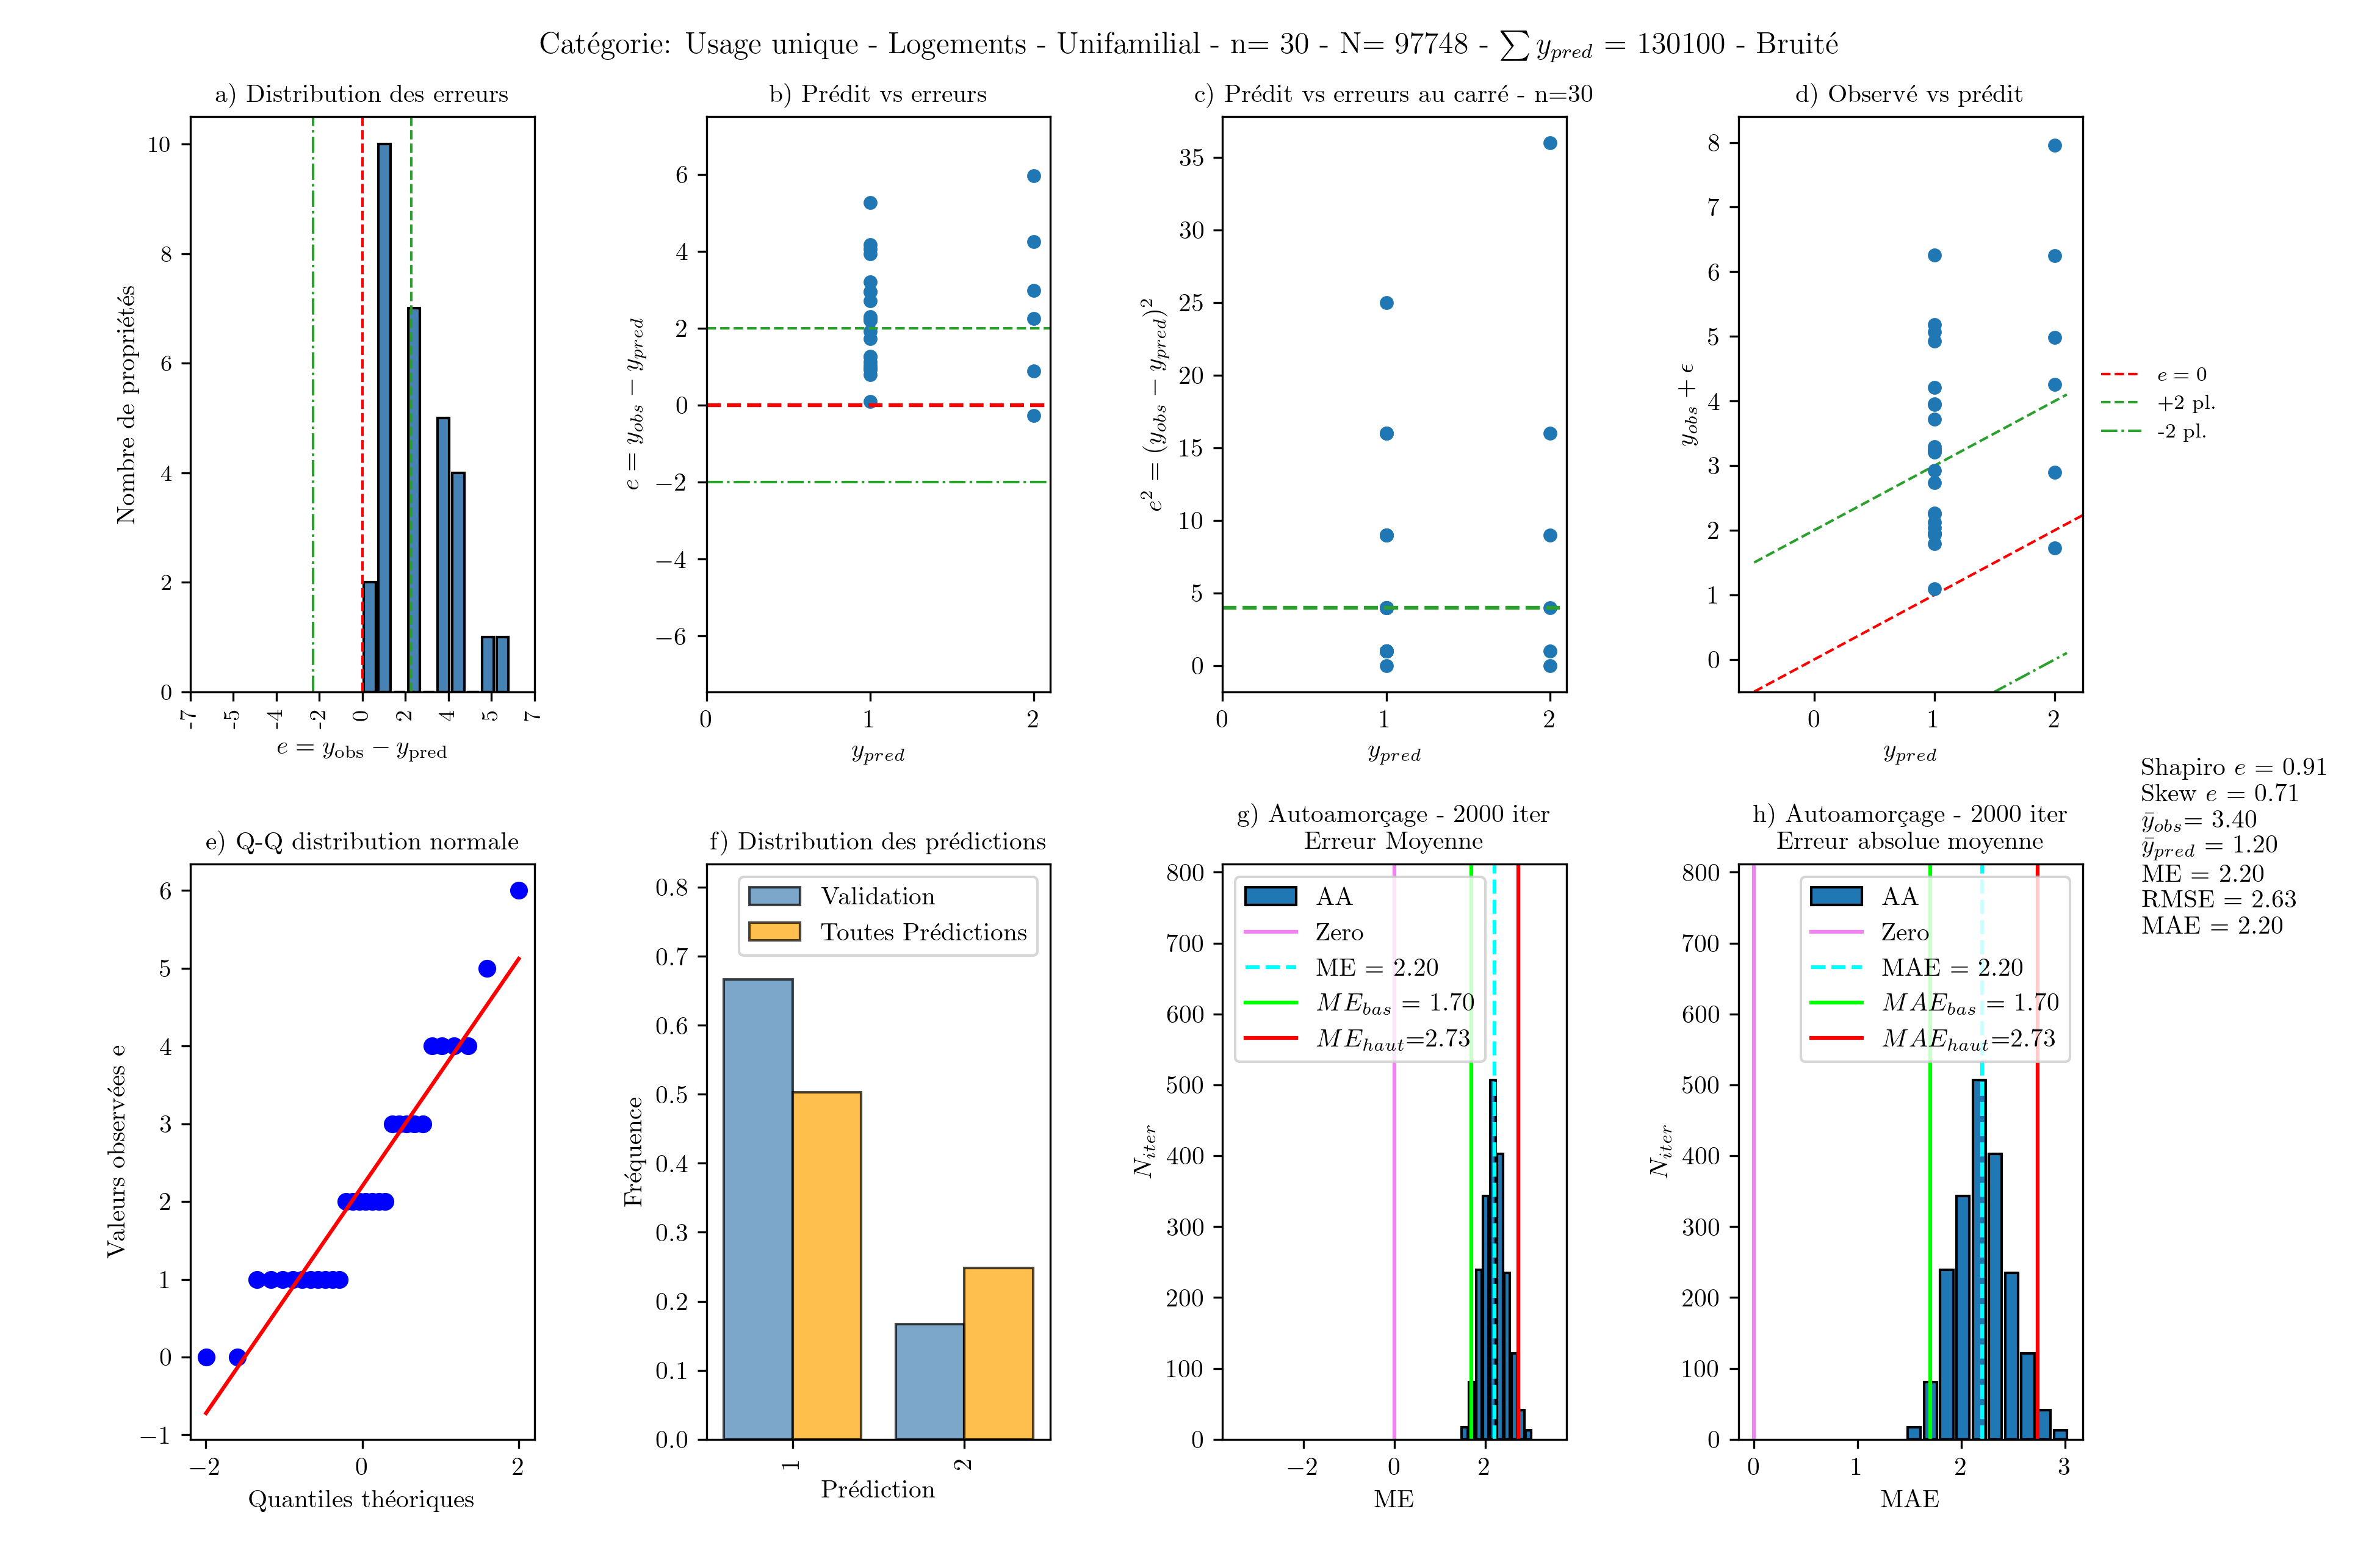
\includegraphics[scale=0.7]{images/int_erreur_36_b_se_2.png}
    %    \caption{Distribution et intervalles de prédiction d'erreur pour le %logement unifamilial}
    %    \label{fig:intervals-dist-val-log-uni}
    %\end{figure}
    \begin{figure}[H]
        \centering
        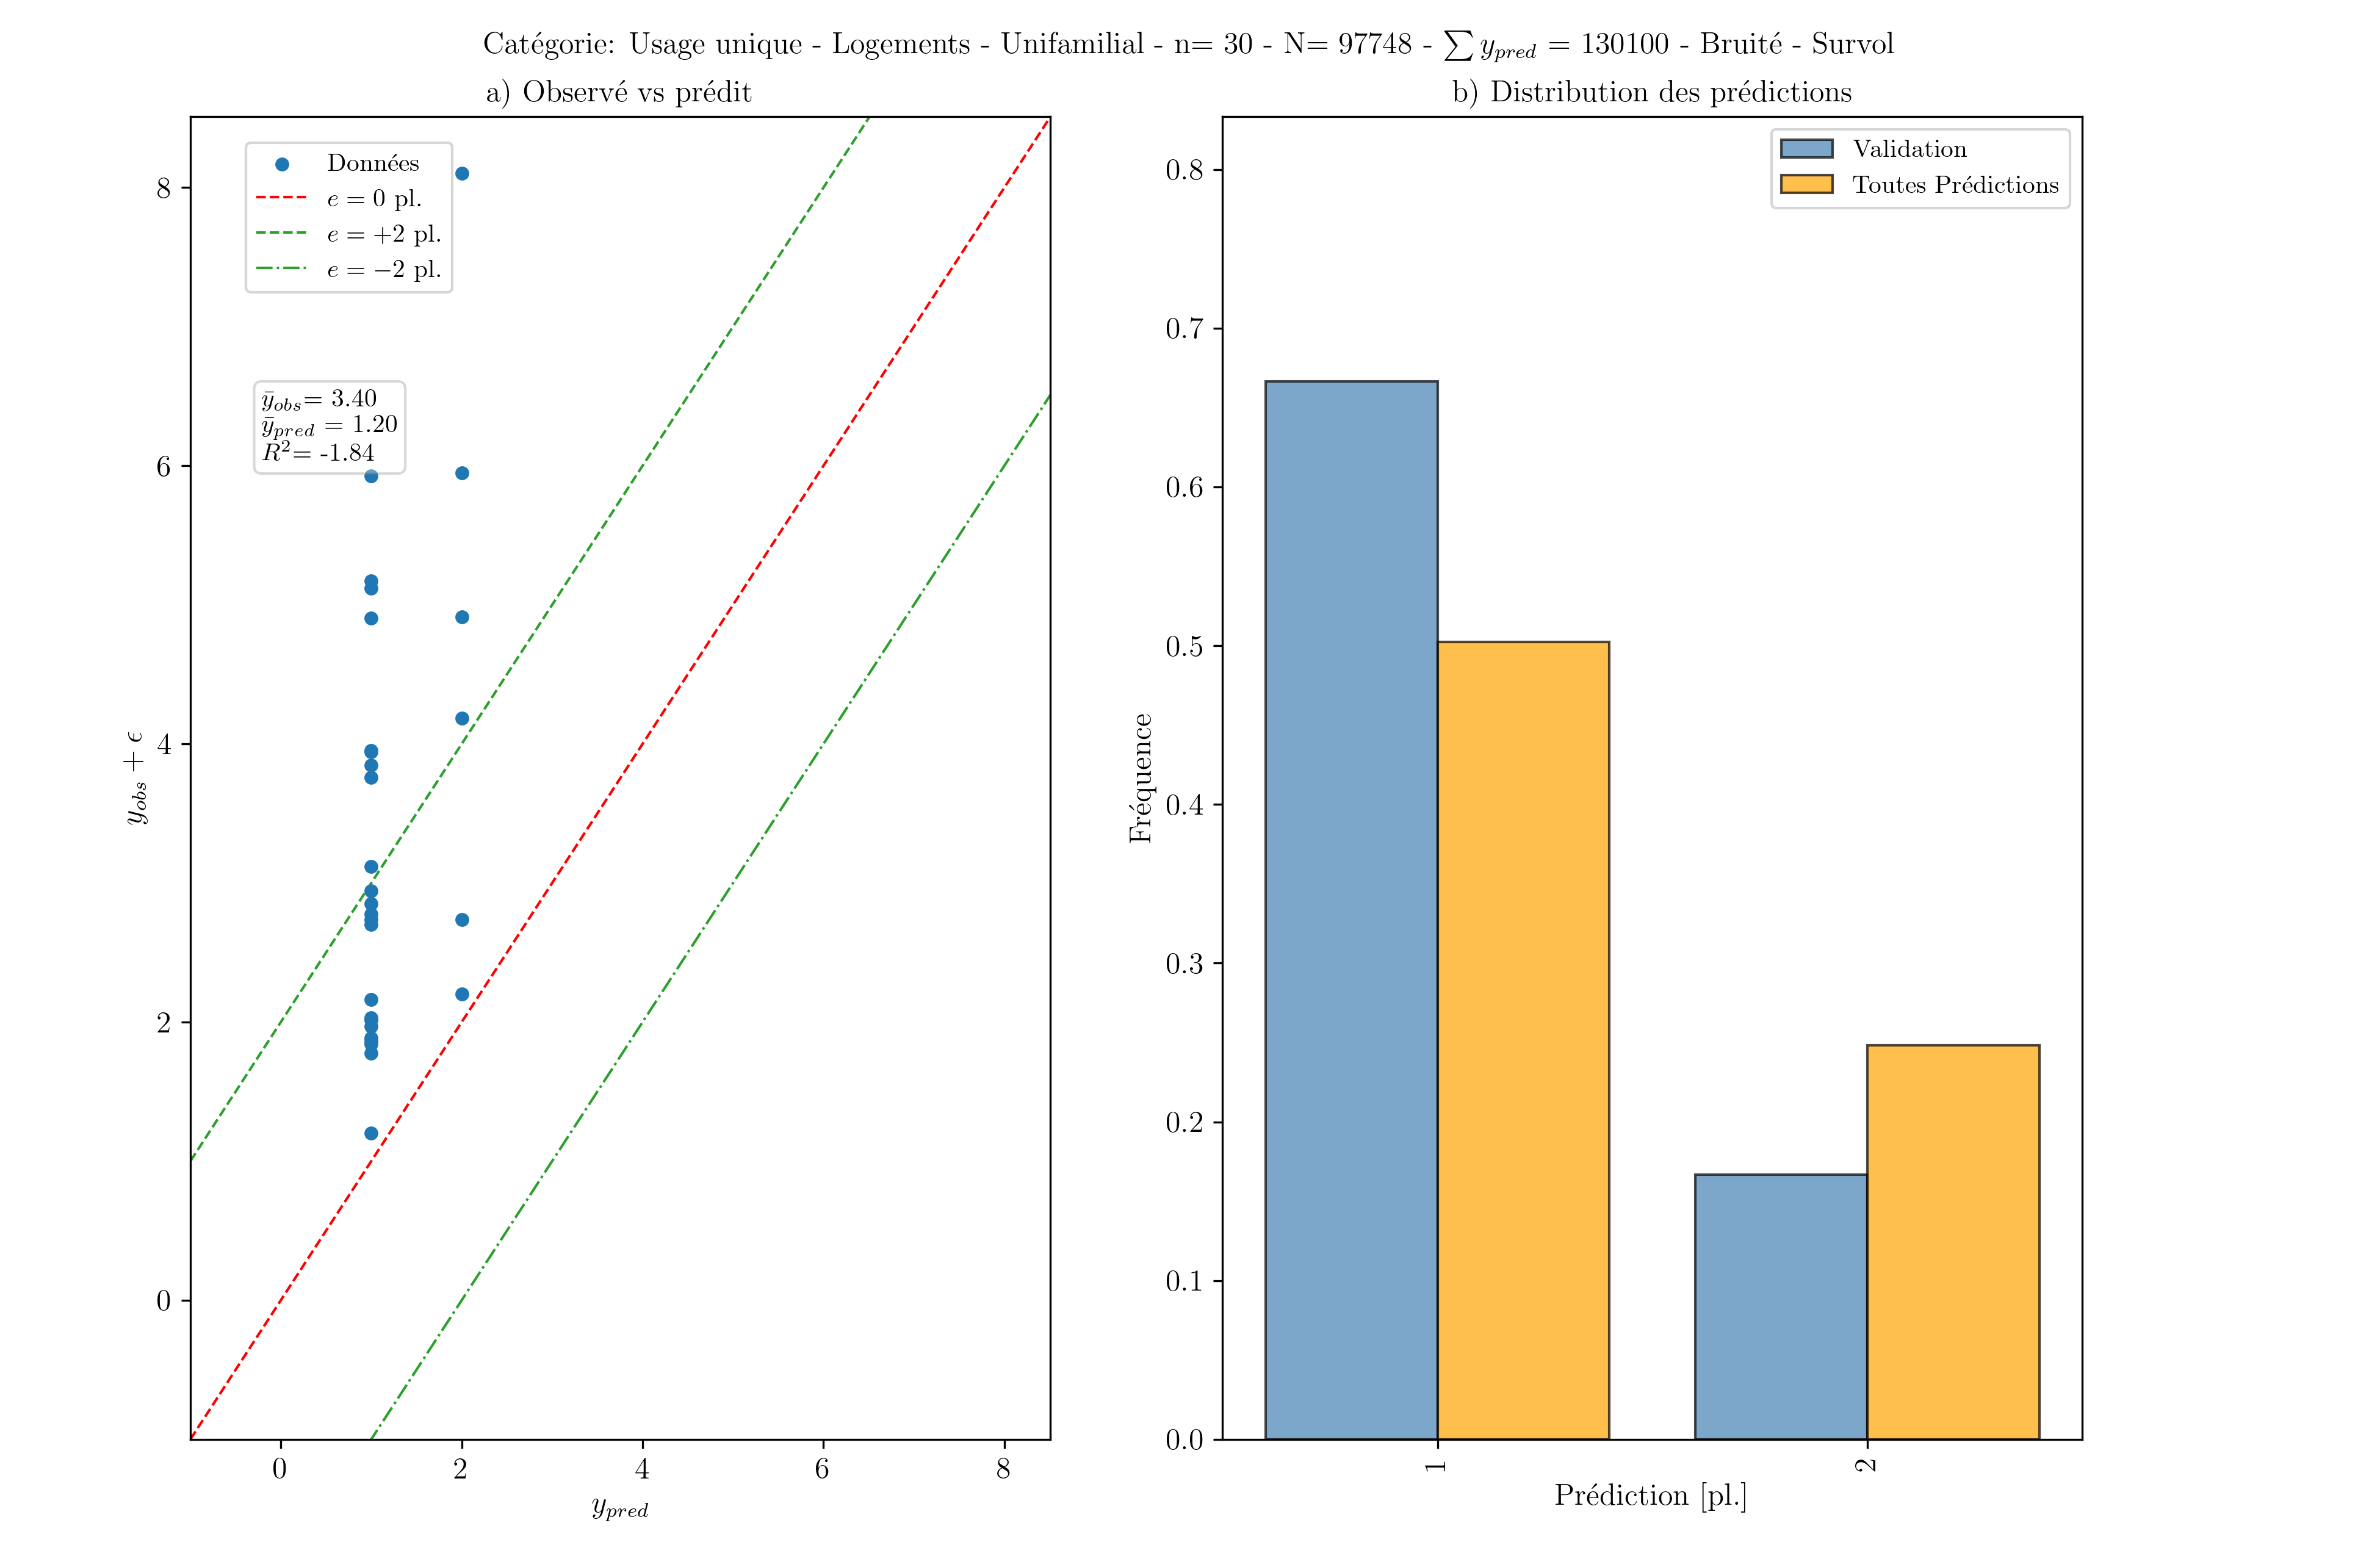
\includegraphics[width=1\linewidth]{images/int_erreur_36_b_se_2_a.png}
        \caption{Distribution des prédictions pour le logement unifamilial}
        \label{fig:int-dist-pred-log-uni}
    \end{figure}
    \begin{figure}[H]
        \centering
        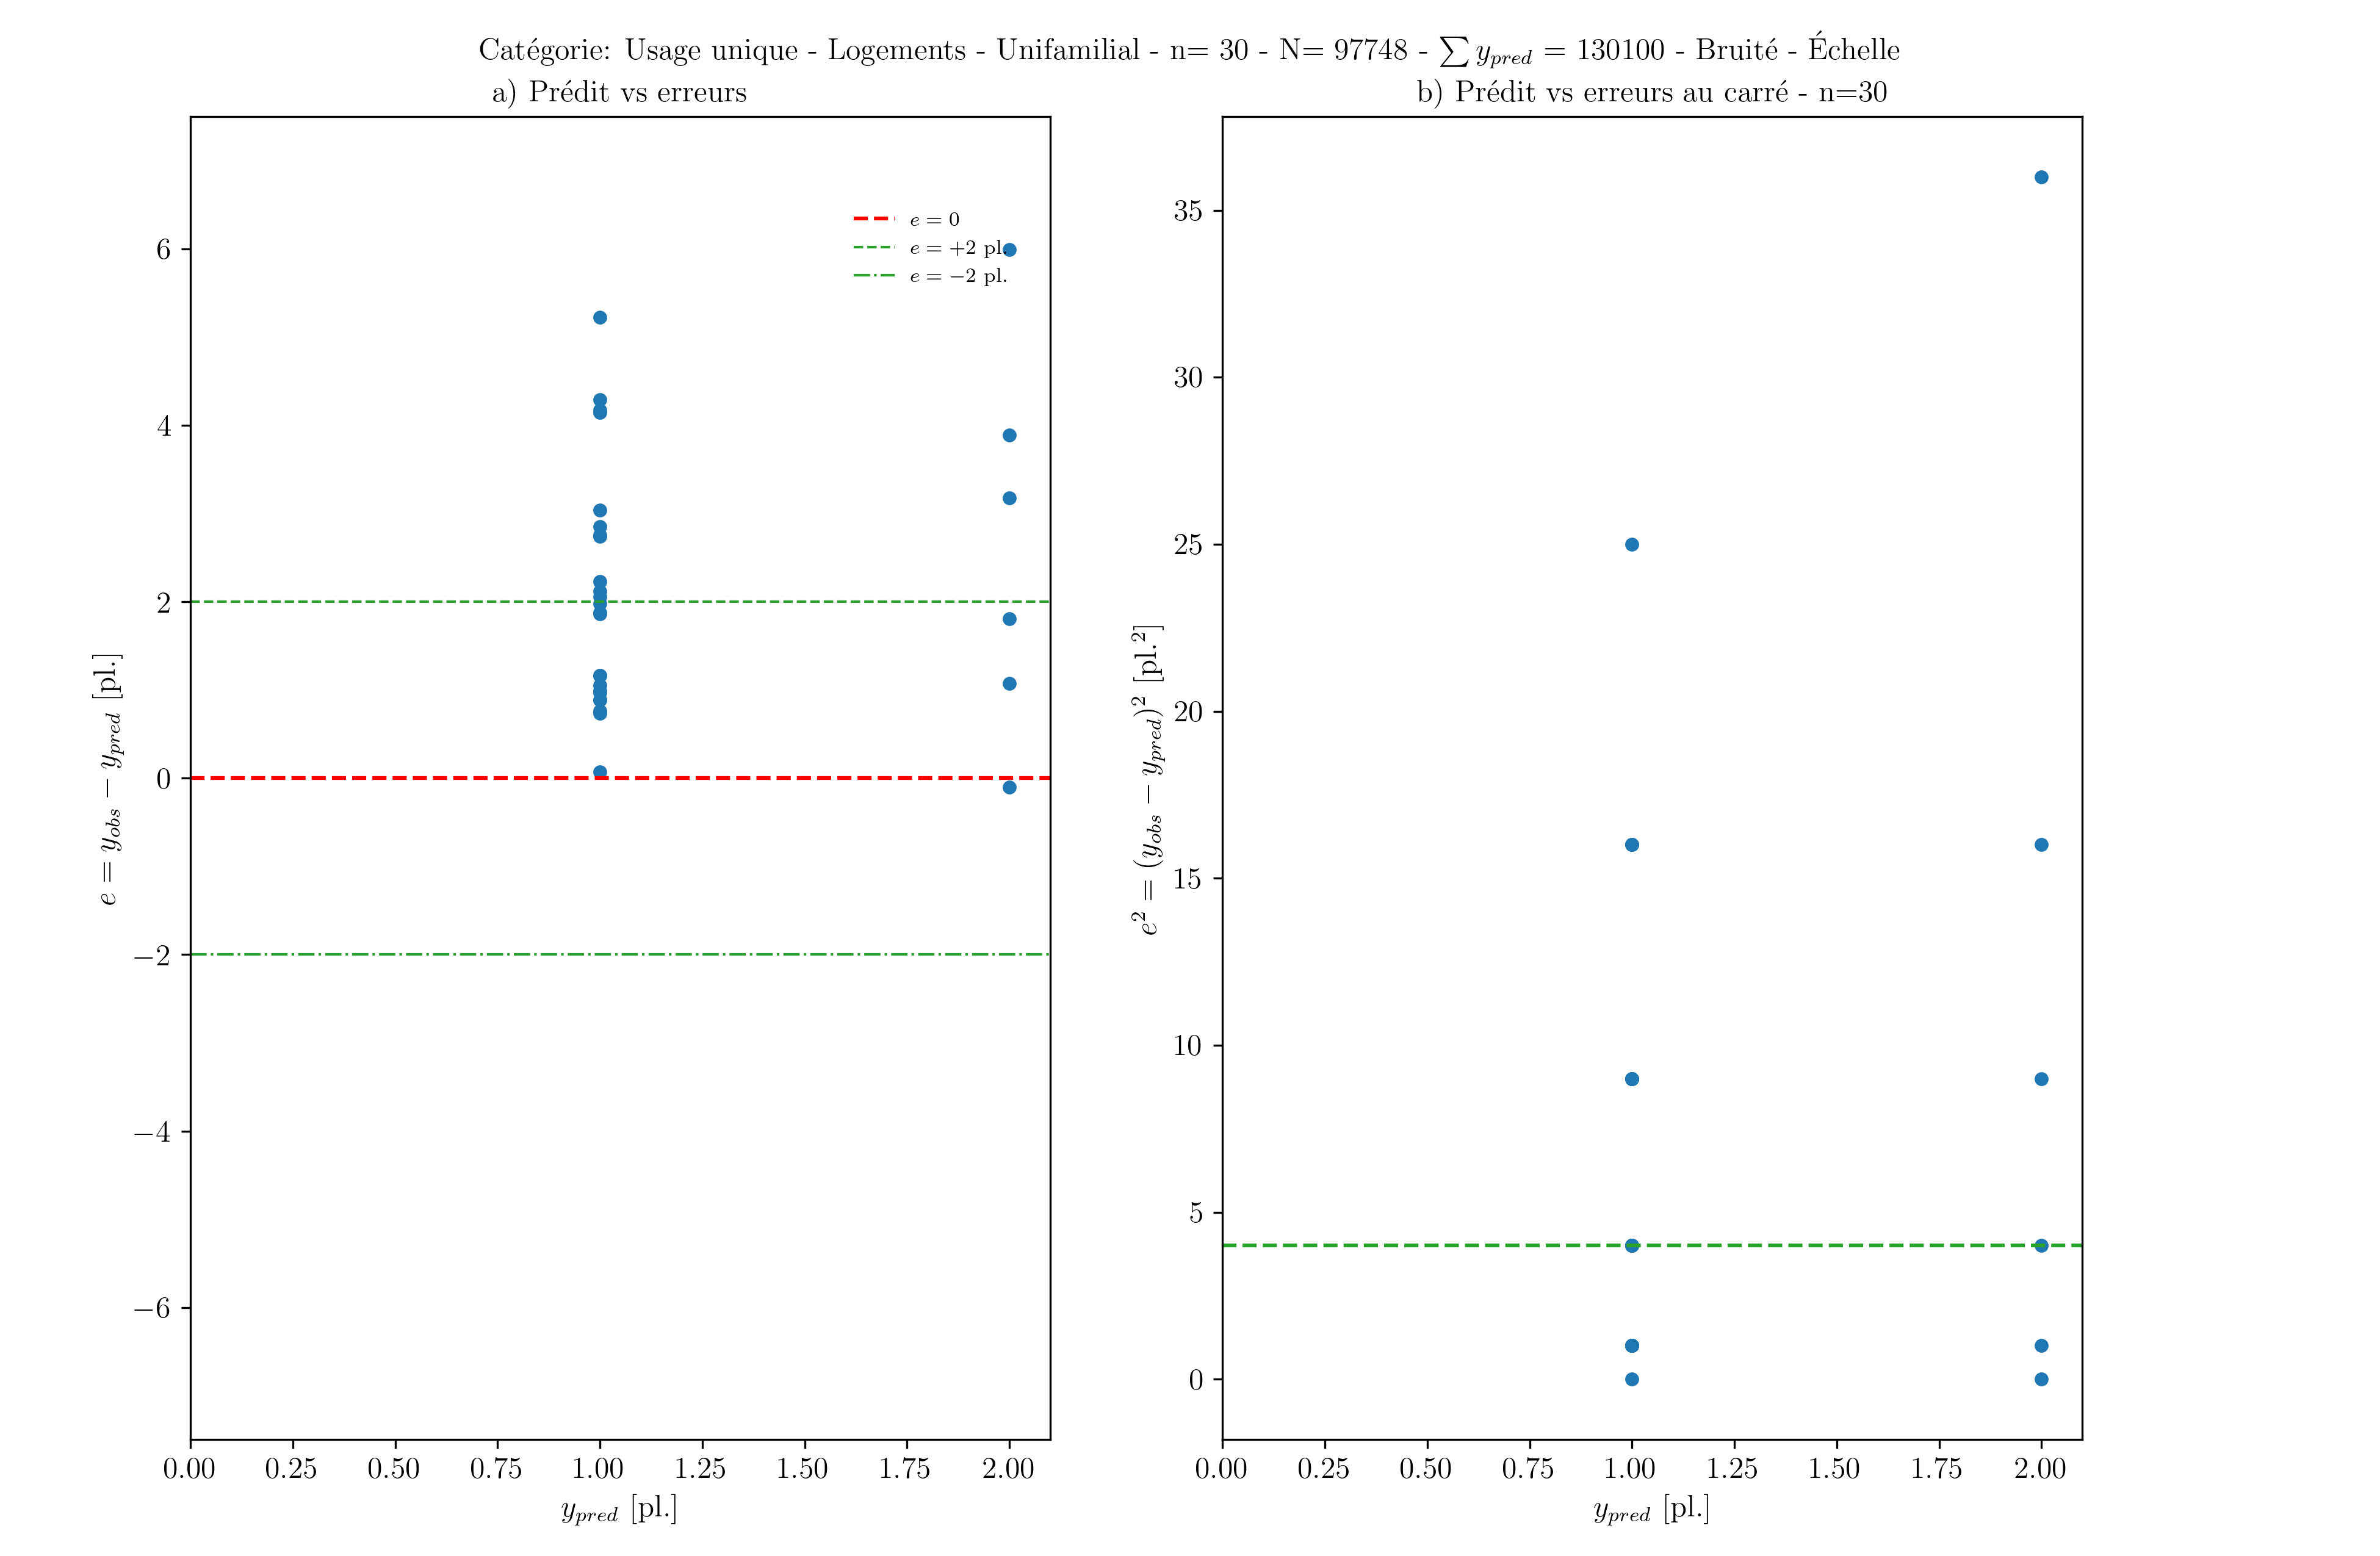
\includegraphics[width=1\linewidth]{images/int_erreur_36_b_se_2_b.png}
        \caption{Erreur en fonction des prédictions pour le logement unifamilial}
        \label{fig:err-err-quad-pred-log-uni}
    \end{figure}
    \begin{figure}[H]
        \centering
        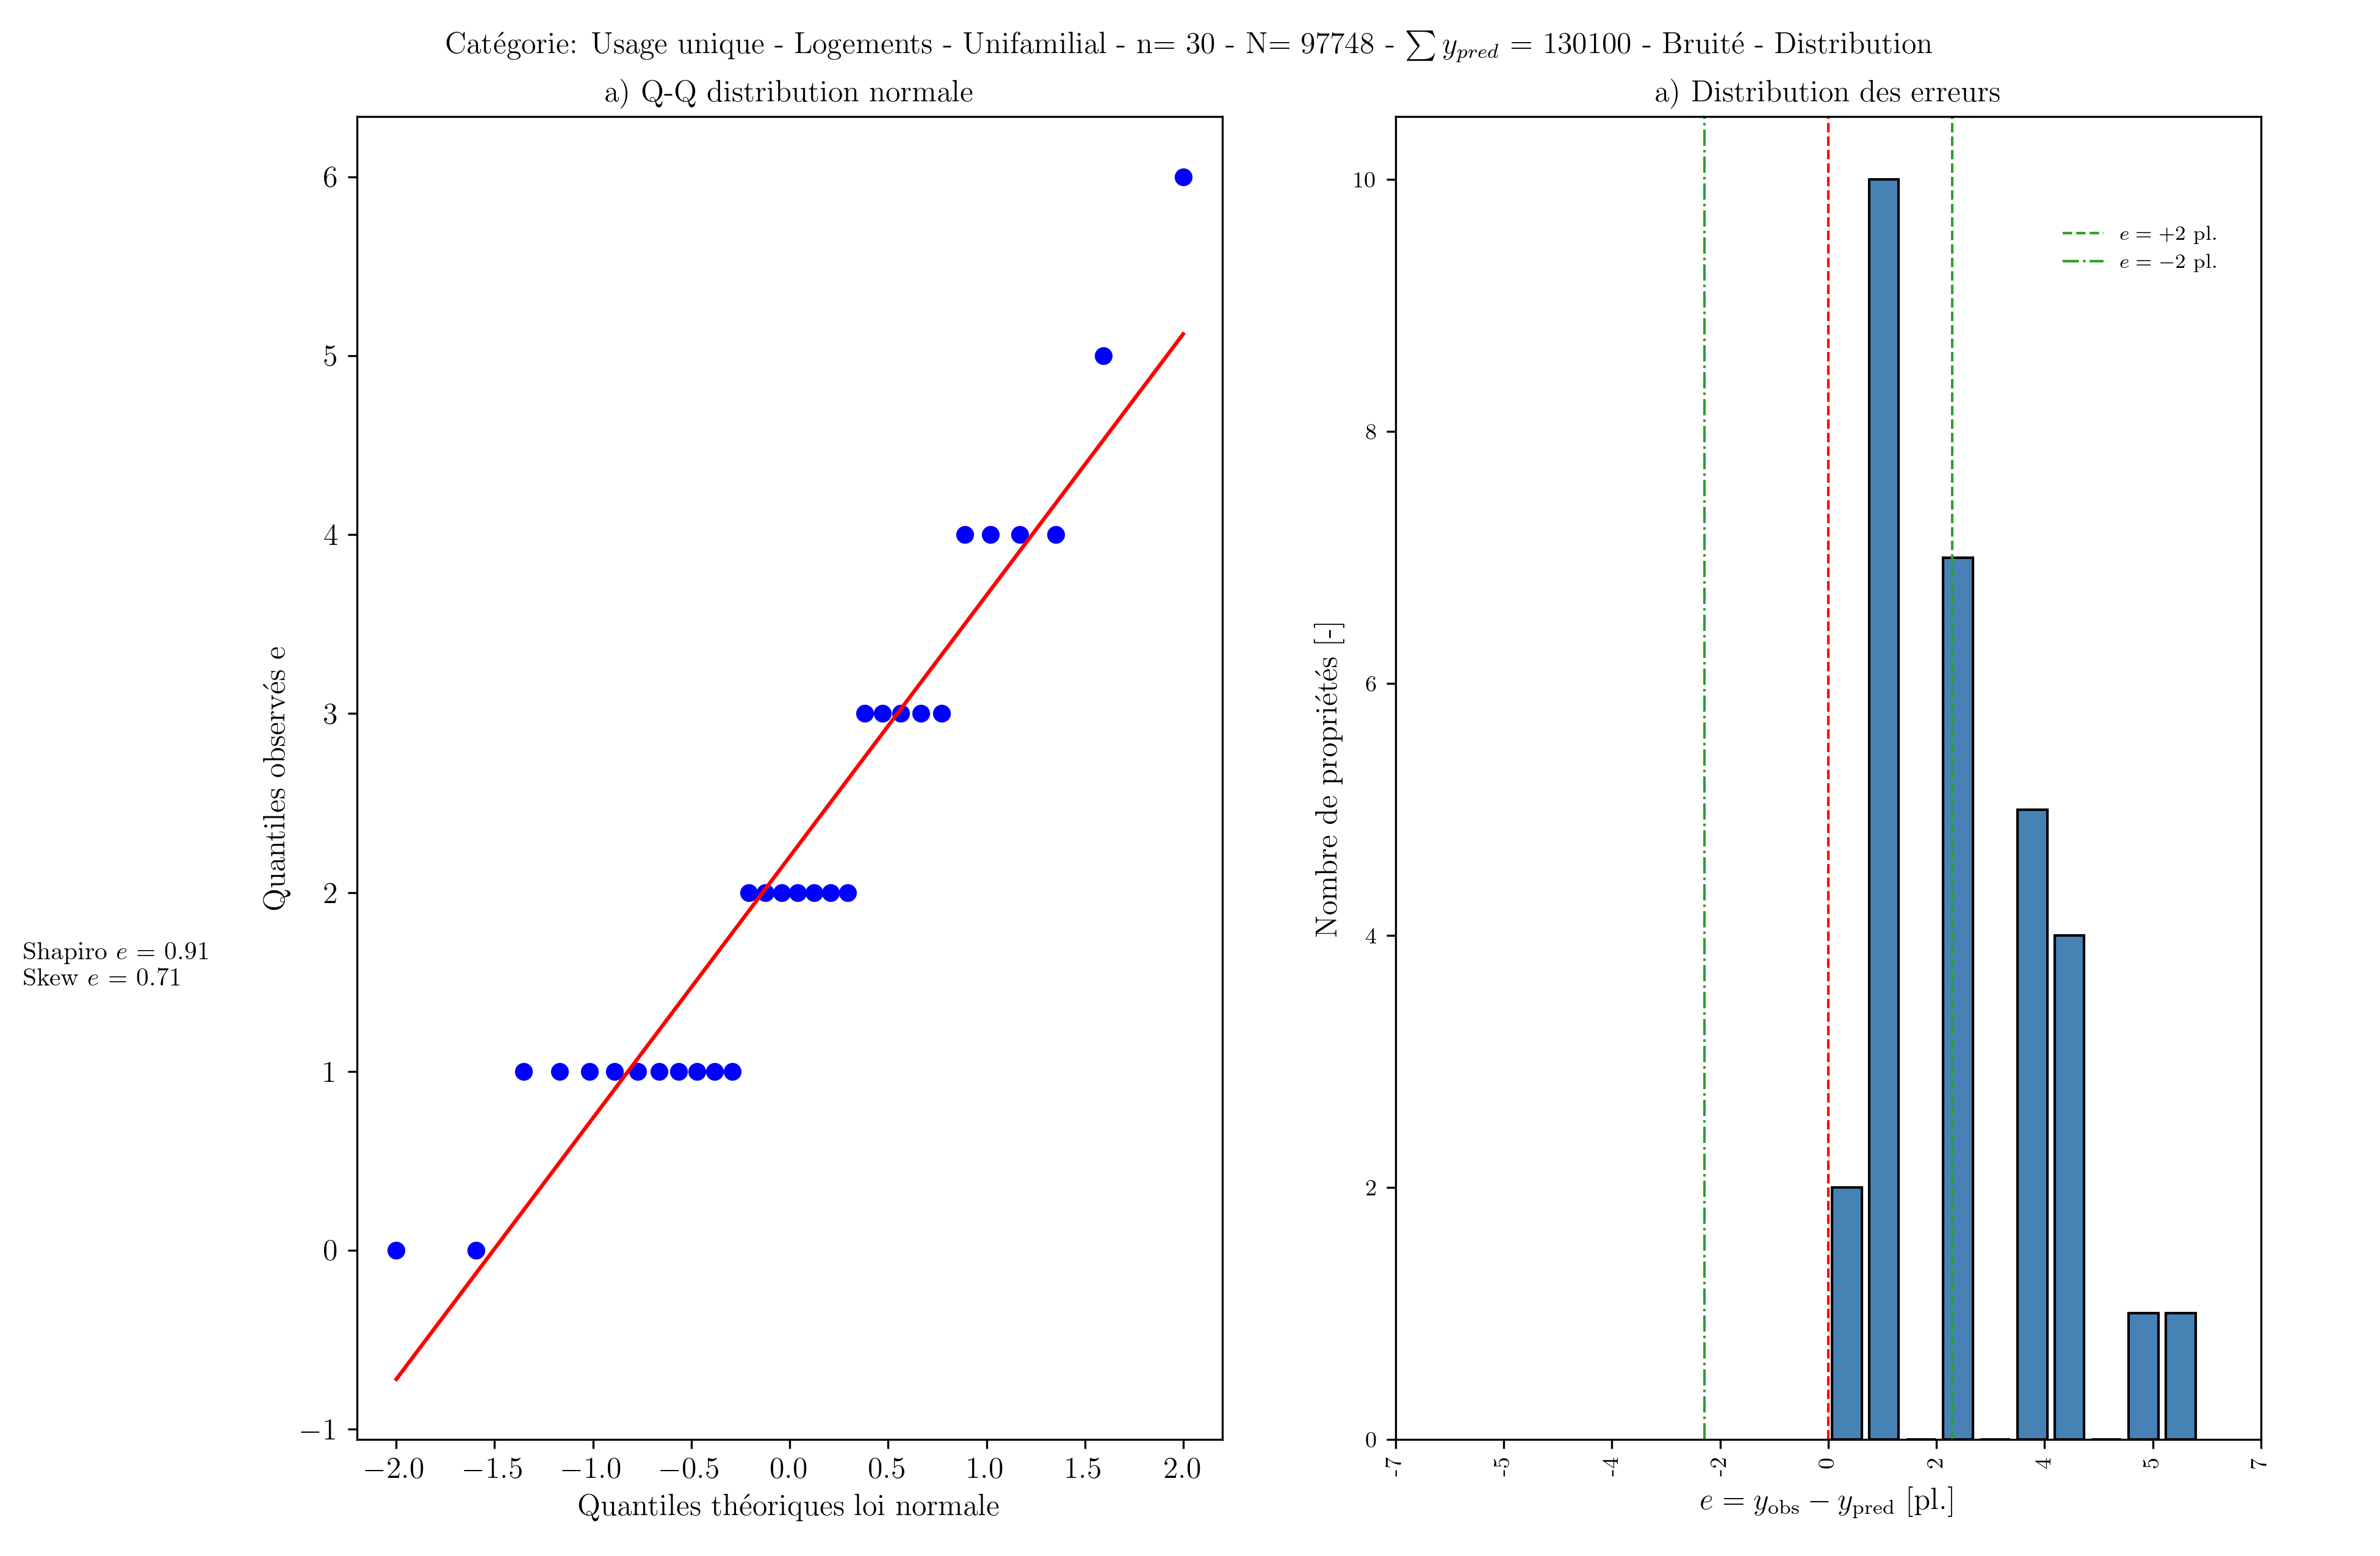
\includegraphics[width=1\linewidth]{images/int_erreur_36_b_se_2_c.png}
        \caption{Distribution et normalité des erreurs pour le logement unifamilial}
        \label{fig:dist-erreur-norm-log-uni}
    \end{figure}
    \begin{figure}[H]
        \centering
        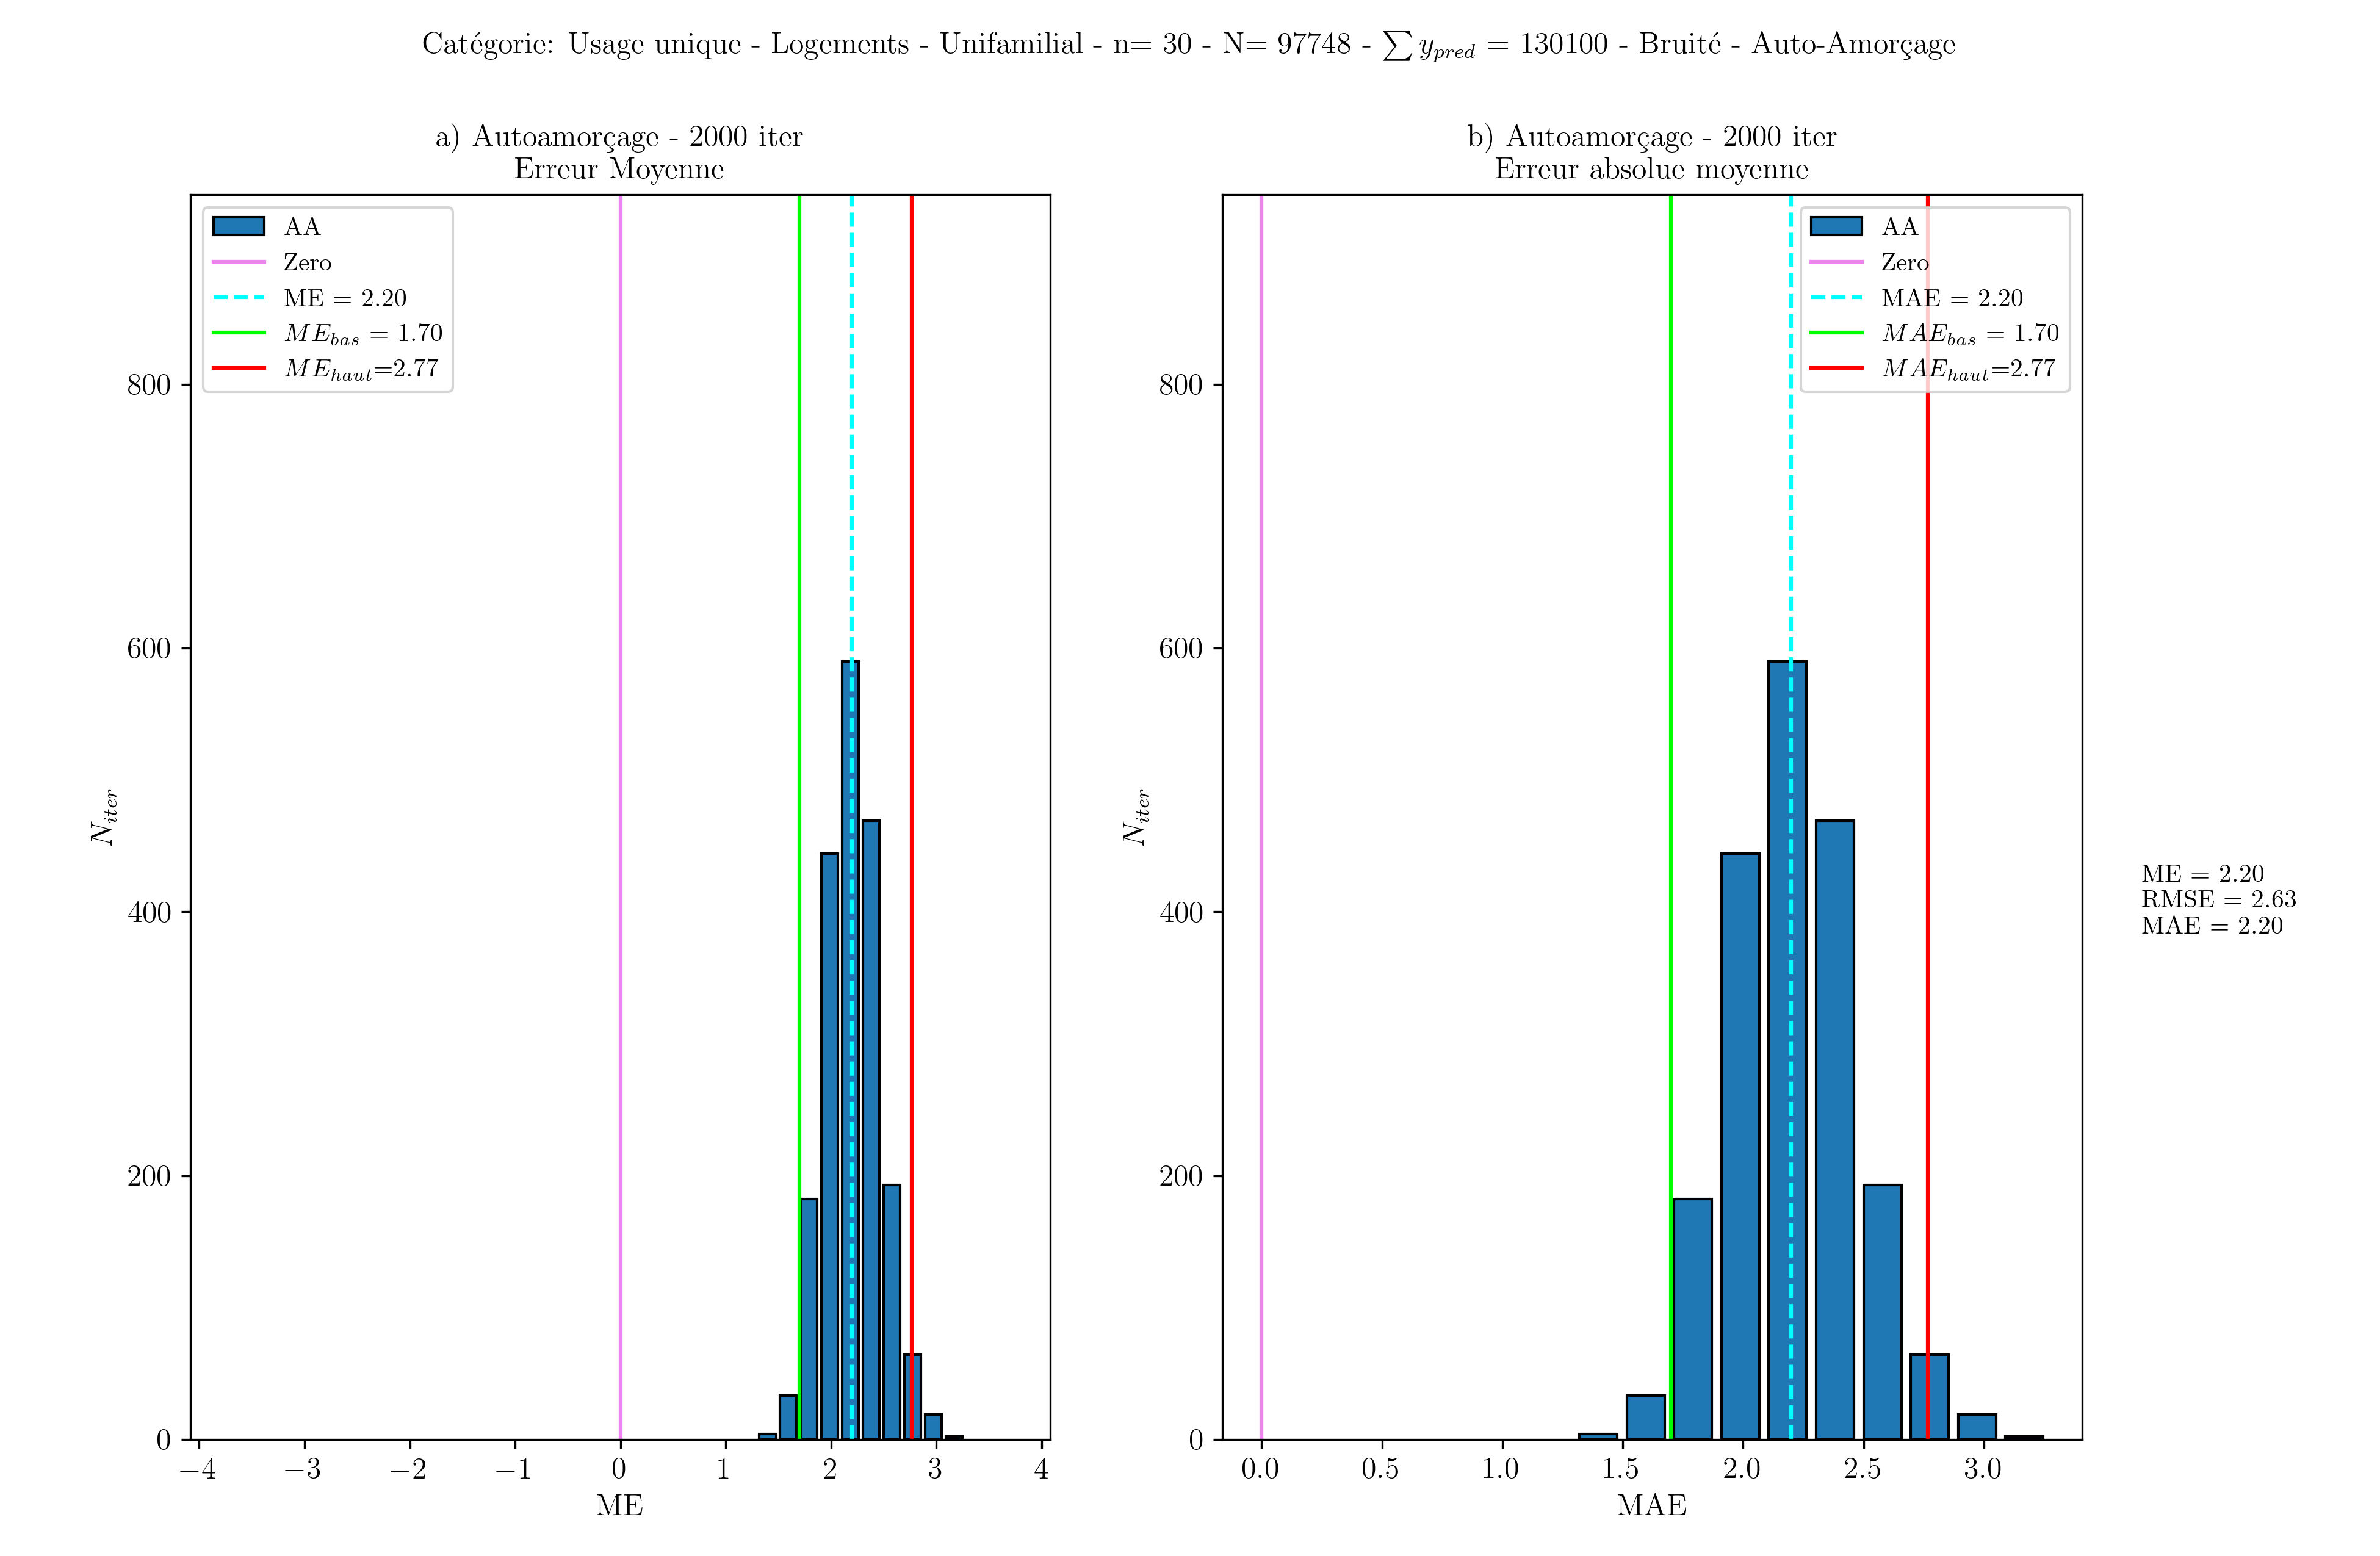
\includegraphics[width=1\linewidth]{images/int_erreur_36_b_se_2_d.png}
        \caption{Distribution des métriques d'erreur après auto-amorçage pour le logement unifamilial}
        \label{fig:auto-amor-log-uni}
    \end{figure}
    %\begin{figure}
    %    \centering
    %    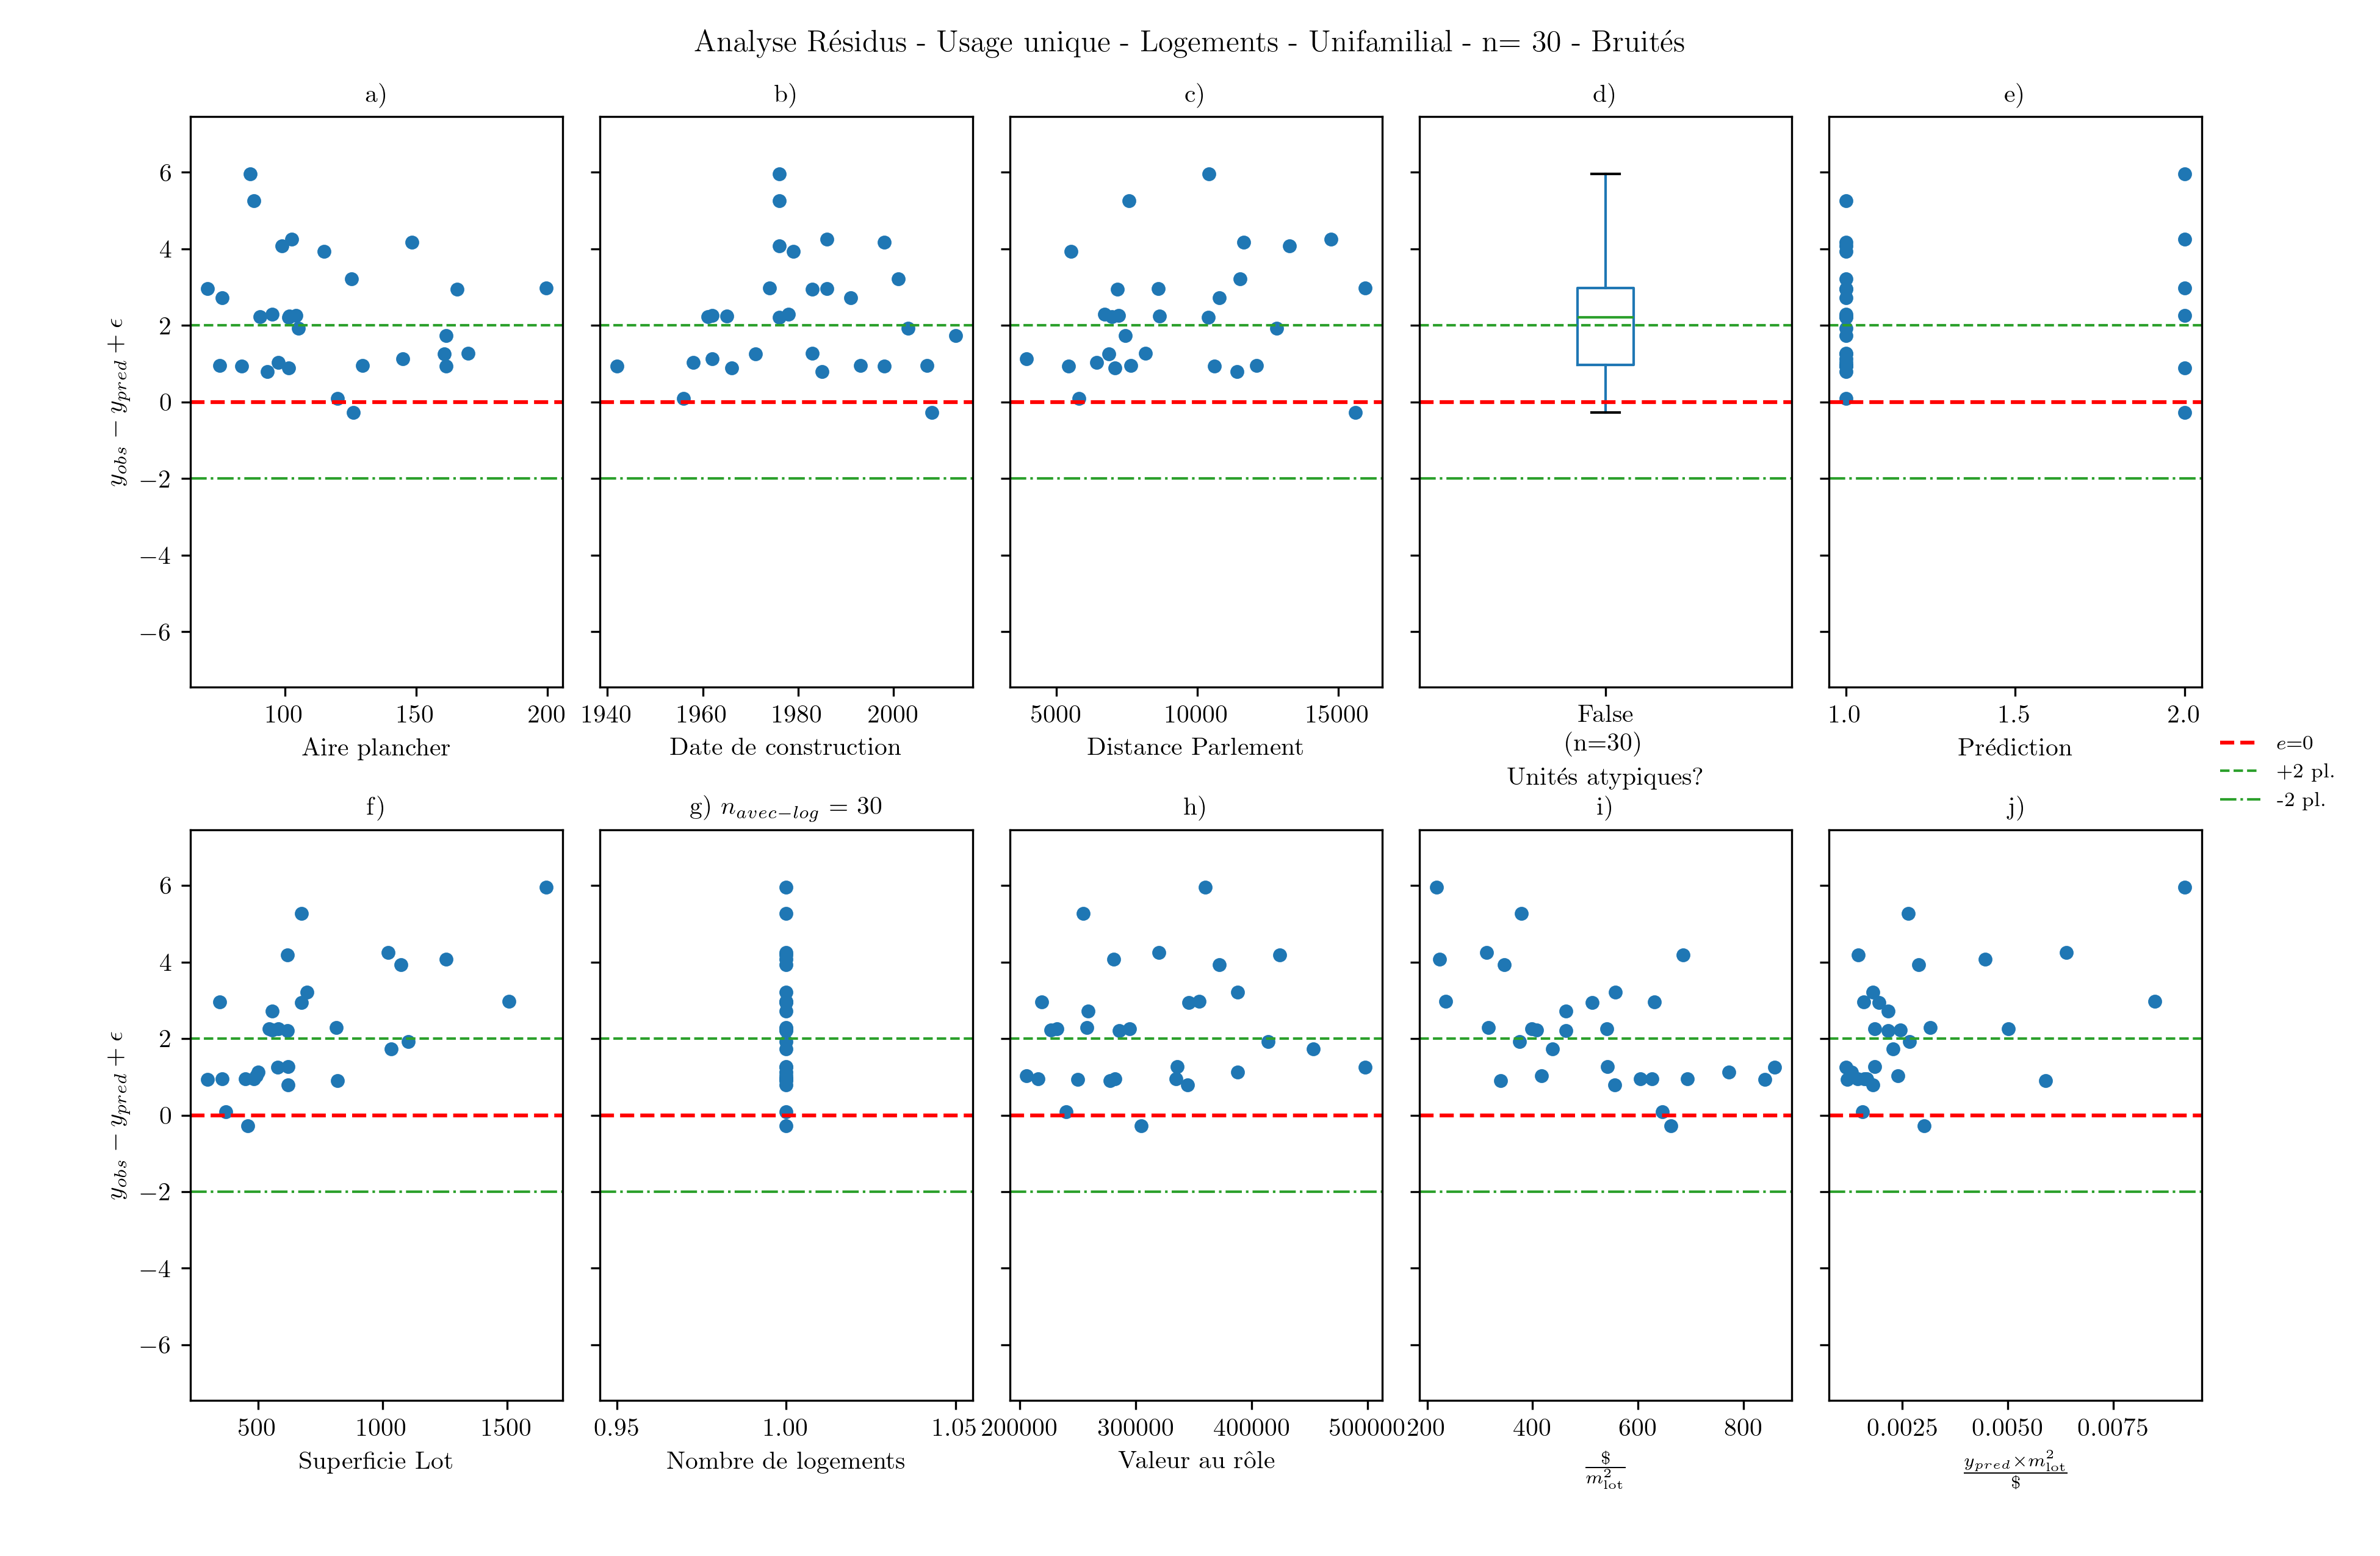
\includegraphics[scale=0.7]{images/ana_res_36_b_se_2.png}
    %    \caption{Analyse des résidus de la prédiction pour le logement unifamilial}
    %    \label{fig:ana-residu-log-uni}
    %\end{figure}
    \begin{figure}[H]
        \centering
        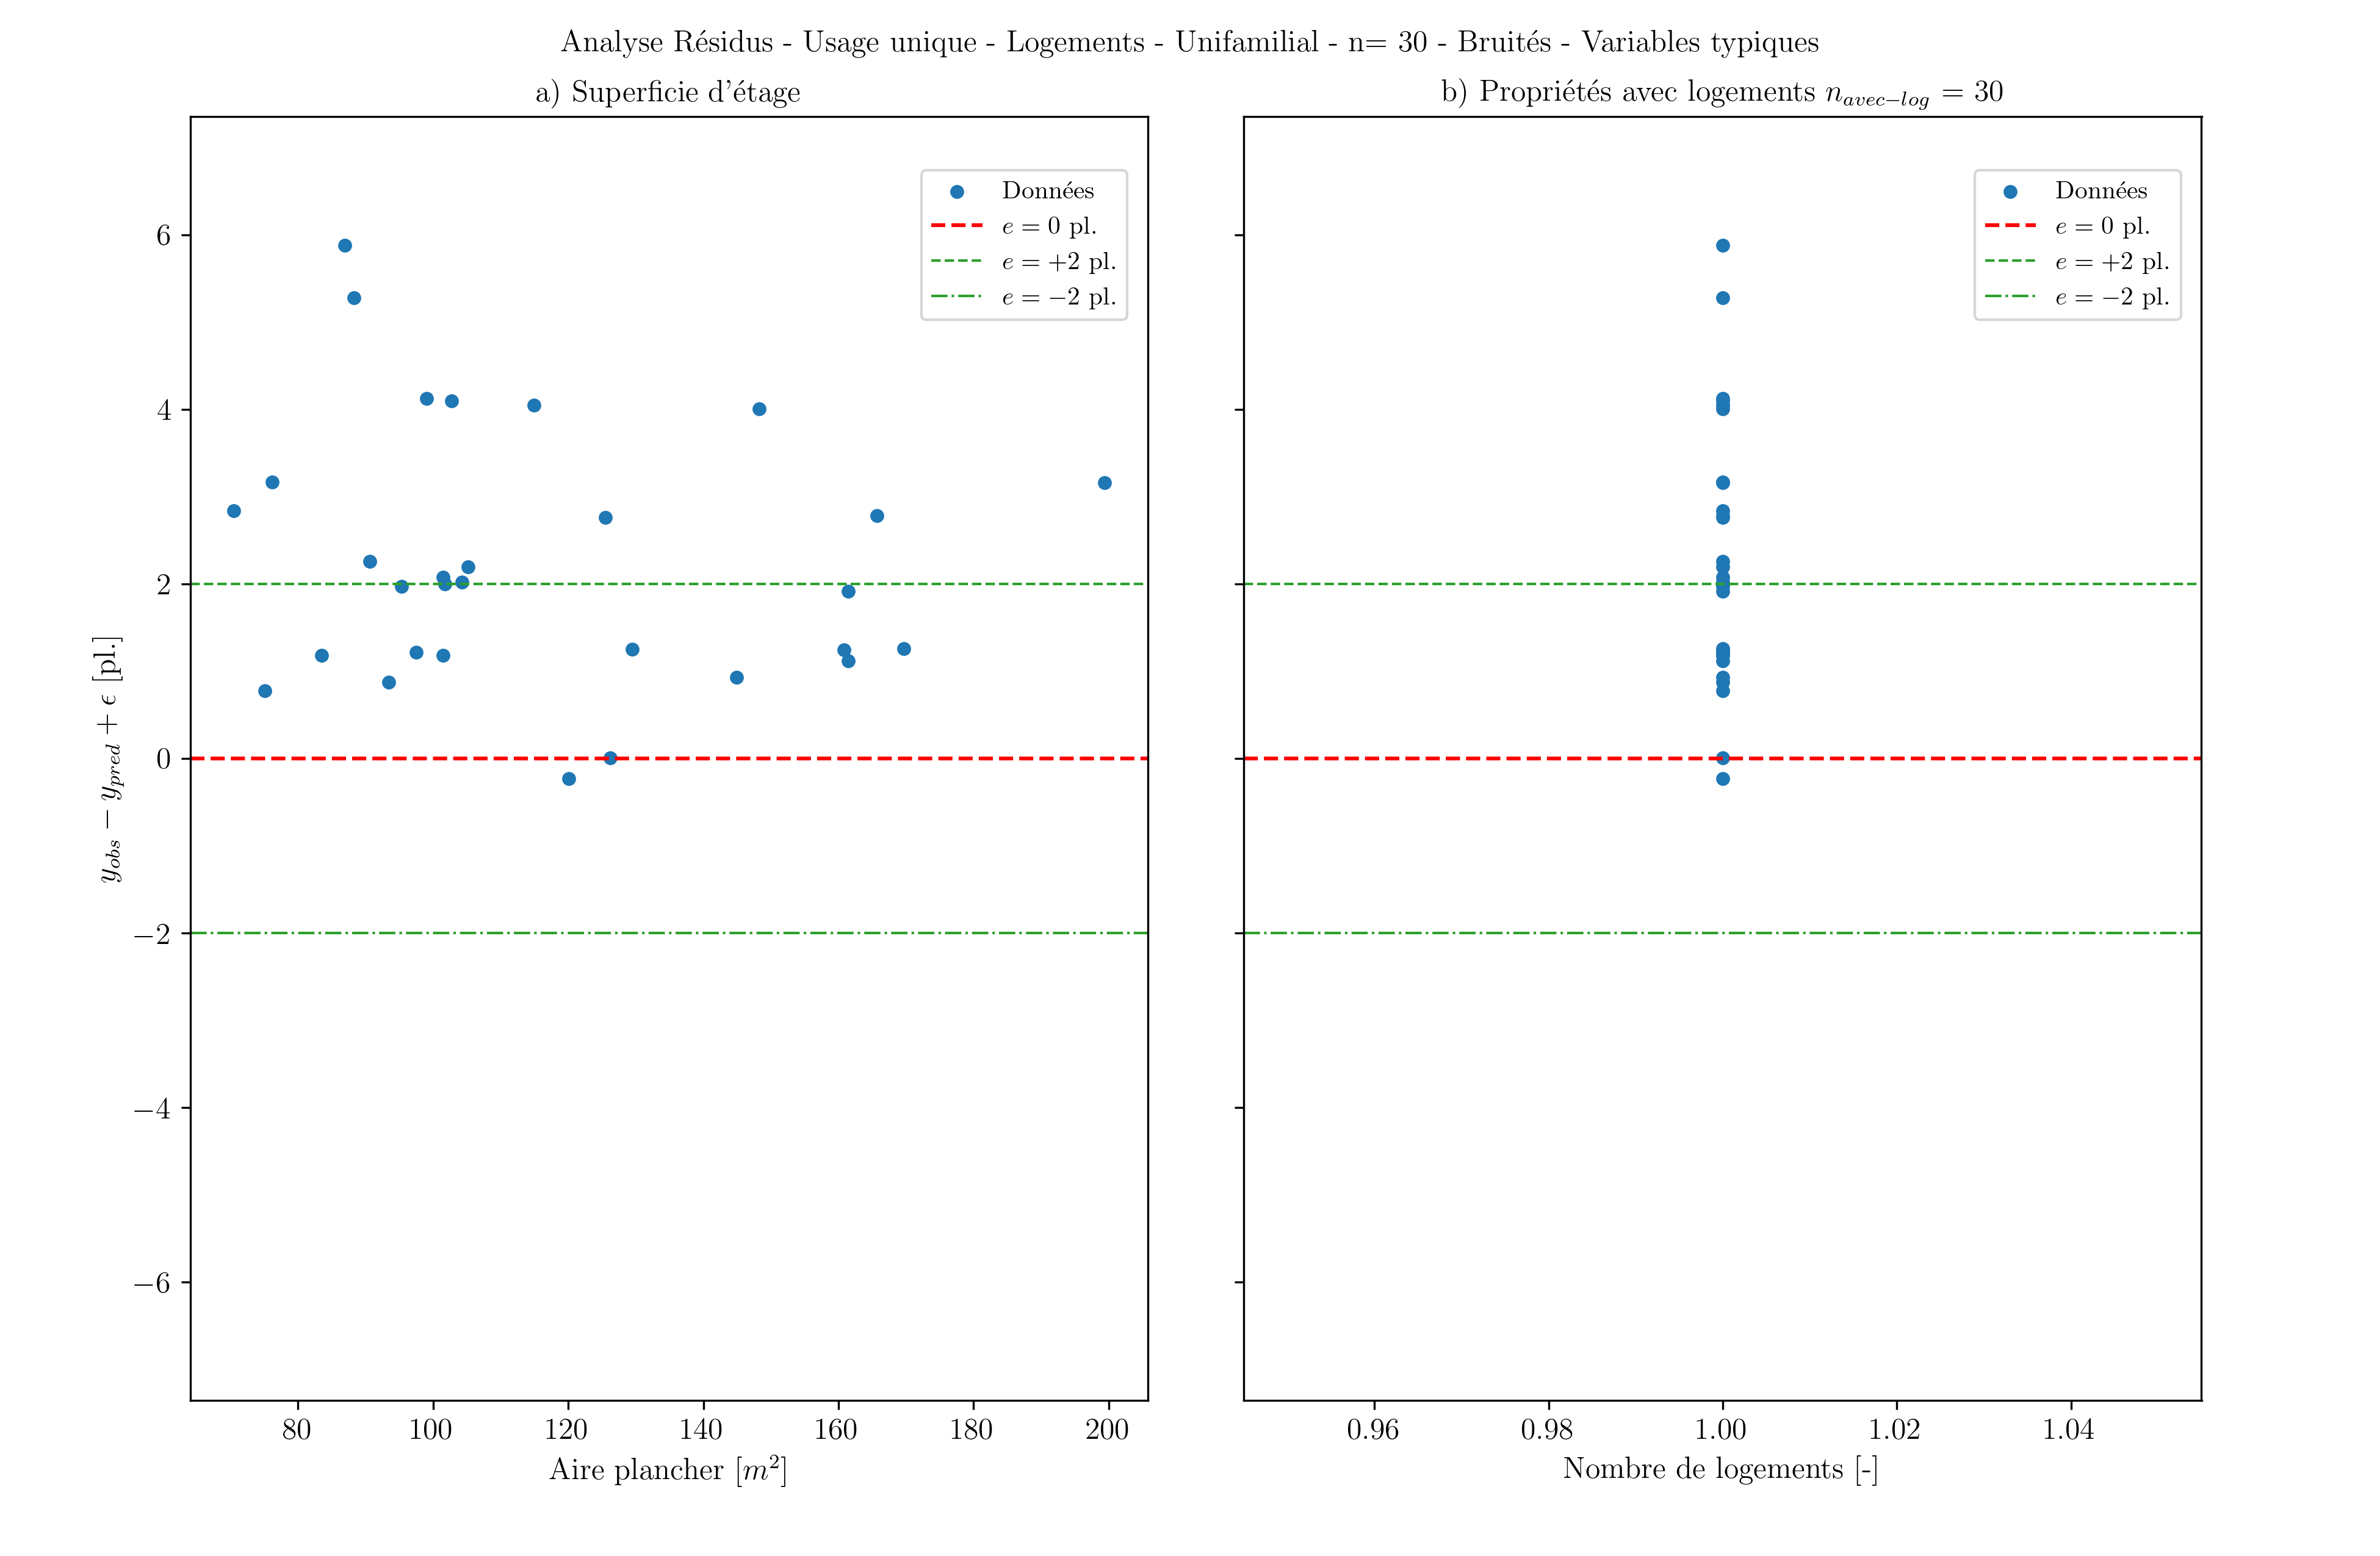
\includegraphics[width=1\linewidth]{images/ana_res_36_b_se_2_a.png}
        \caption{Analyse des résidus en fonction des propriétés de construction du logement unifamilial}
        \label{fig:ana-res-prop-phys-log-uni}
    \end{figure}
    \begin{figure}[H]
        \centering
        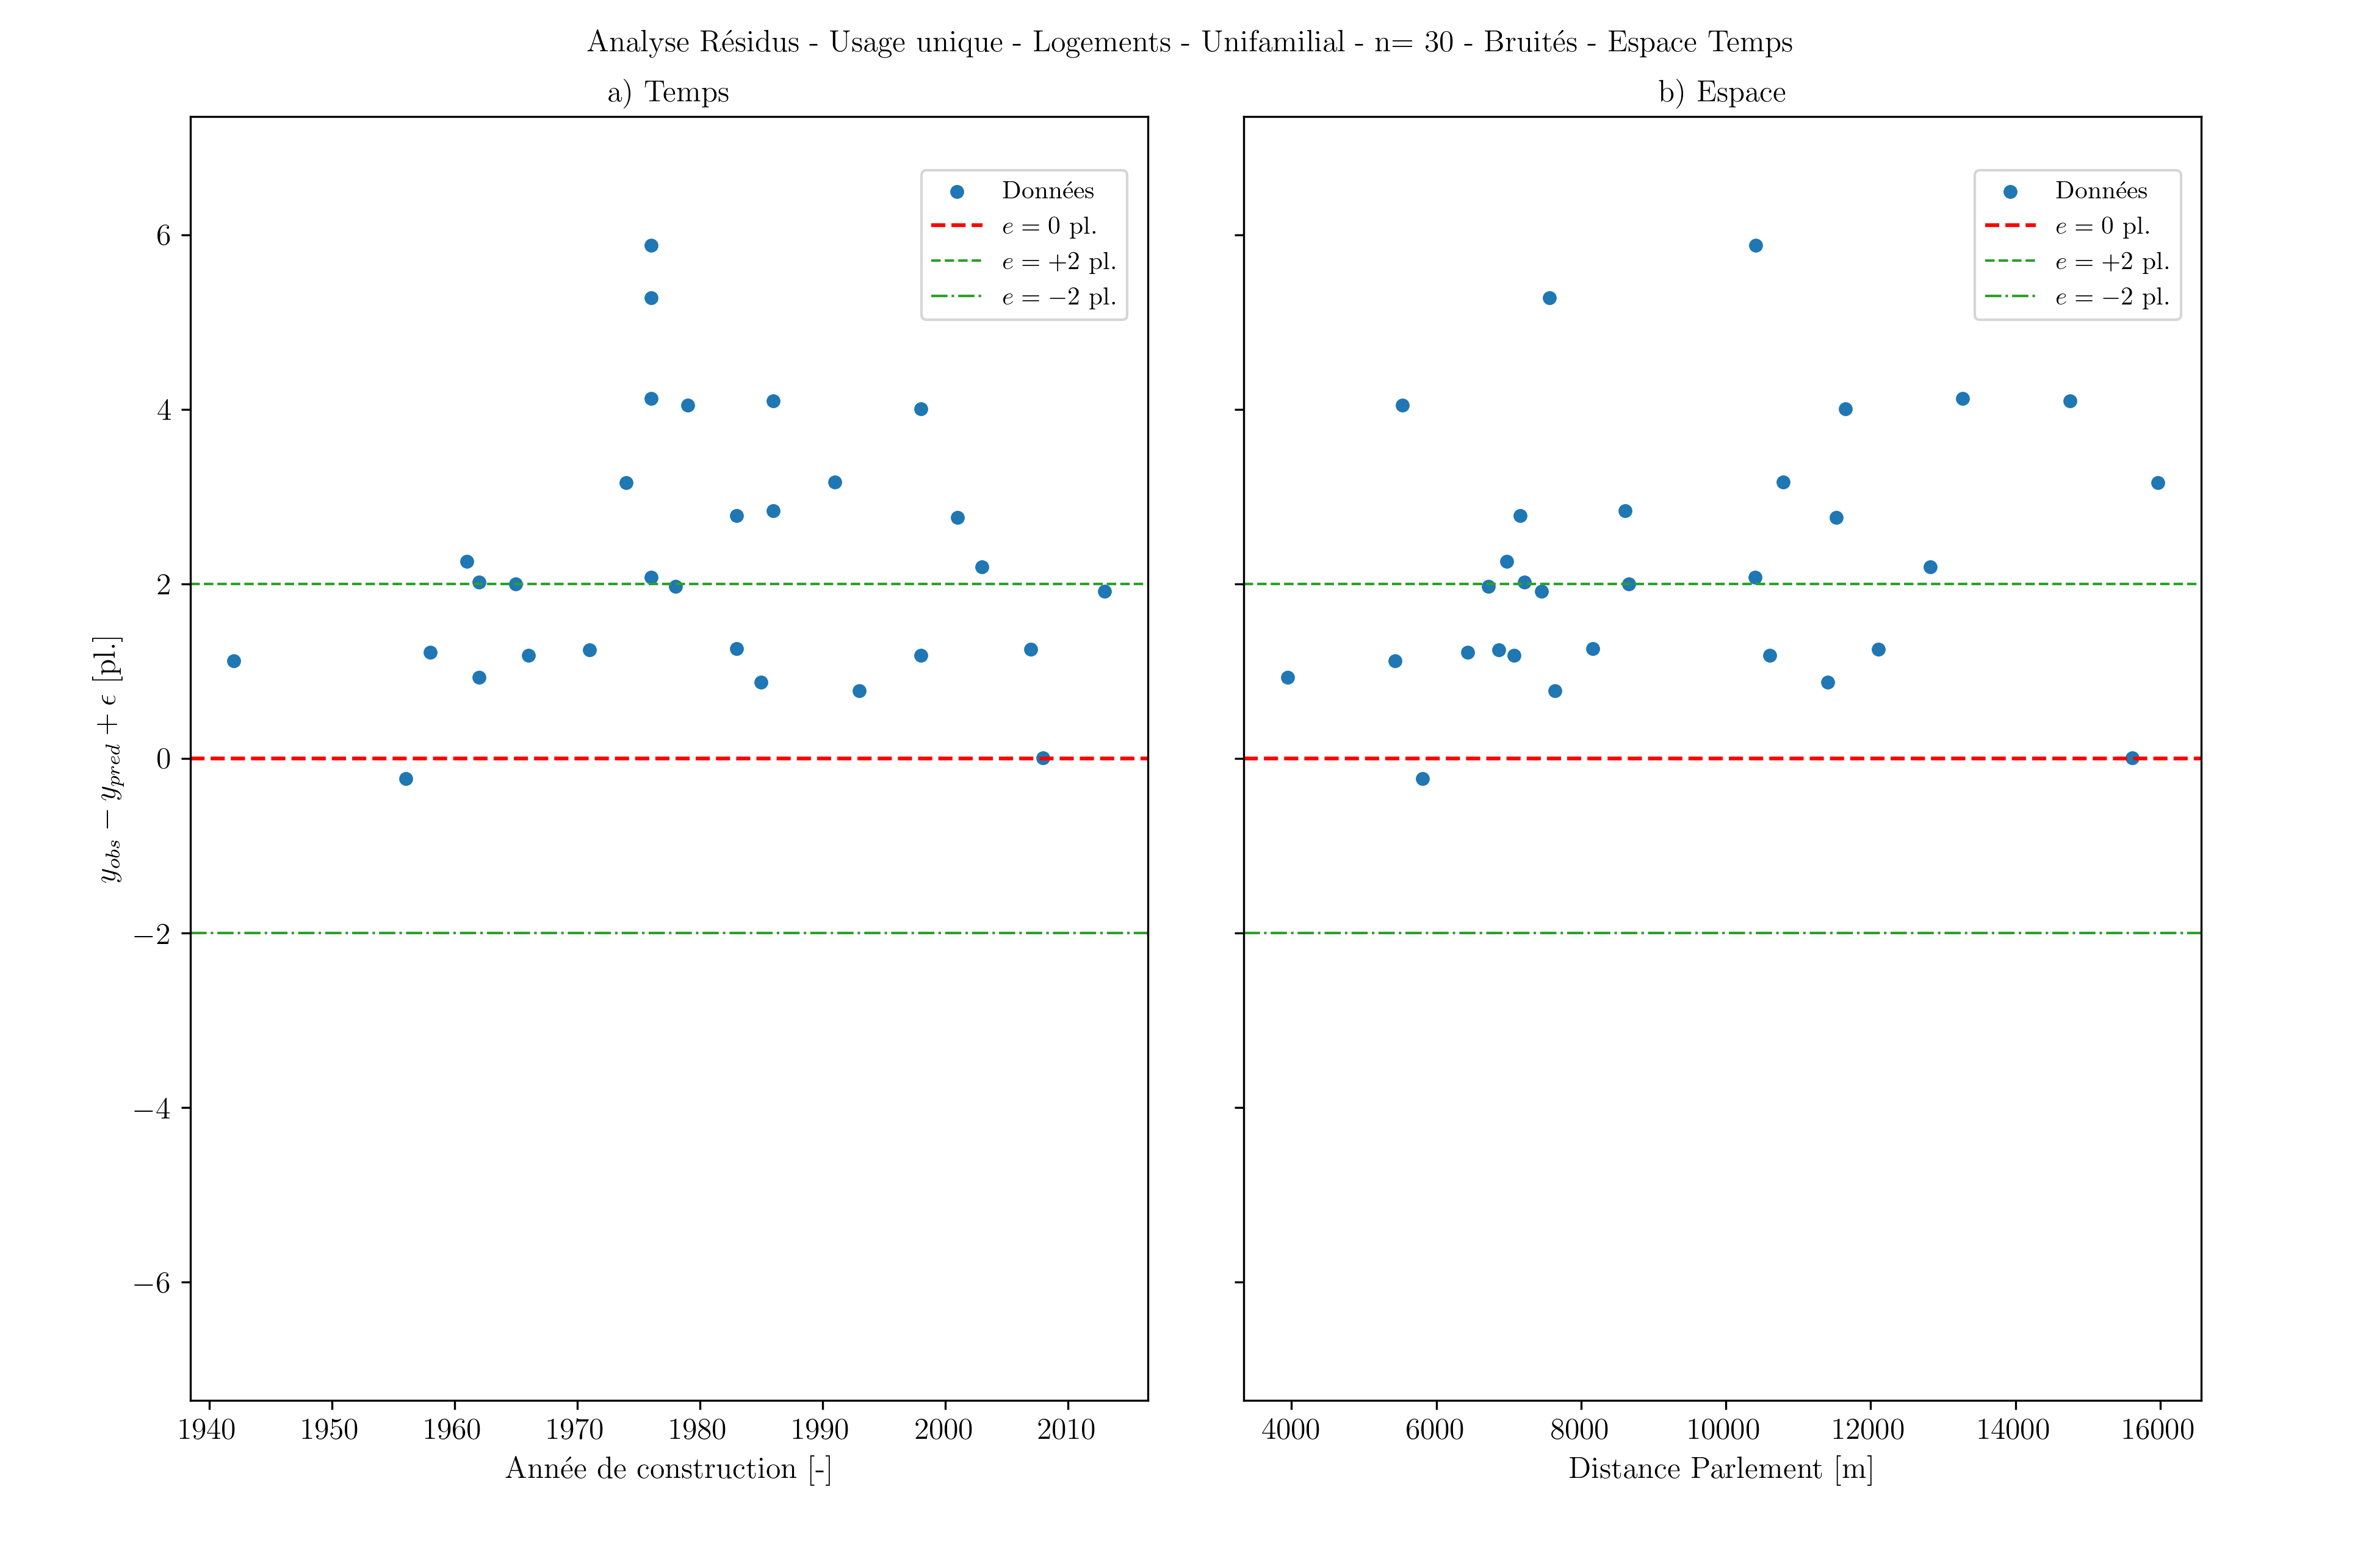
\includegraphics[width=1\linewidth]{images/ana_res_36_b_se_2_b.png}
        \caption{Analyse des résidus en fonction de l'espace et de l'époque de construction pour le logement unifamilial}
        \label{fig:ana-res-esp-temps-log-uni}
    \end{figure}
    \begin{figure}[H]
        \centering
        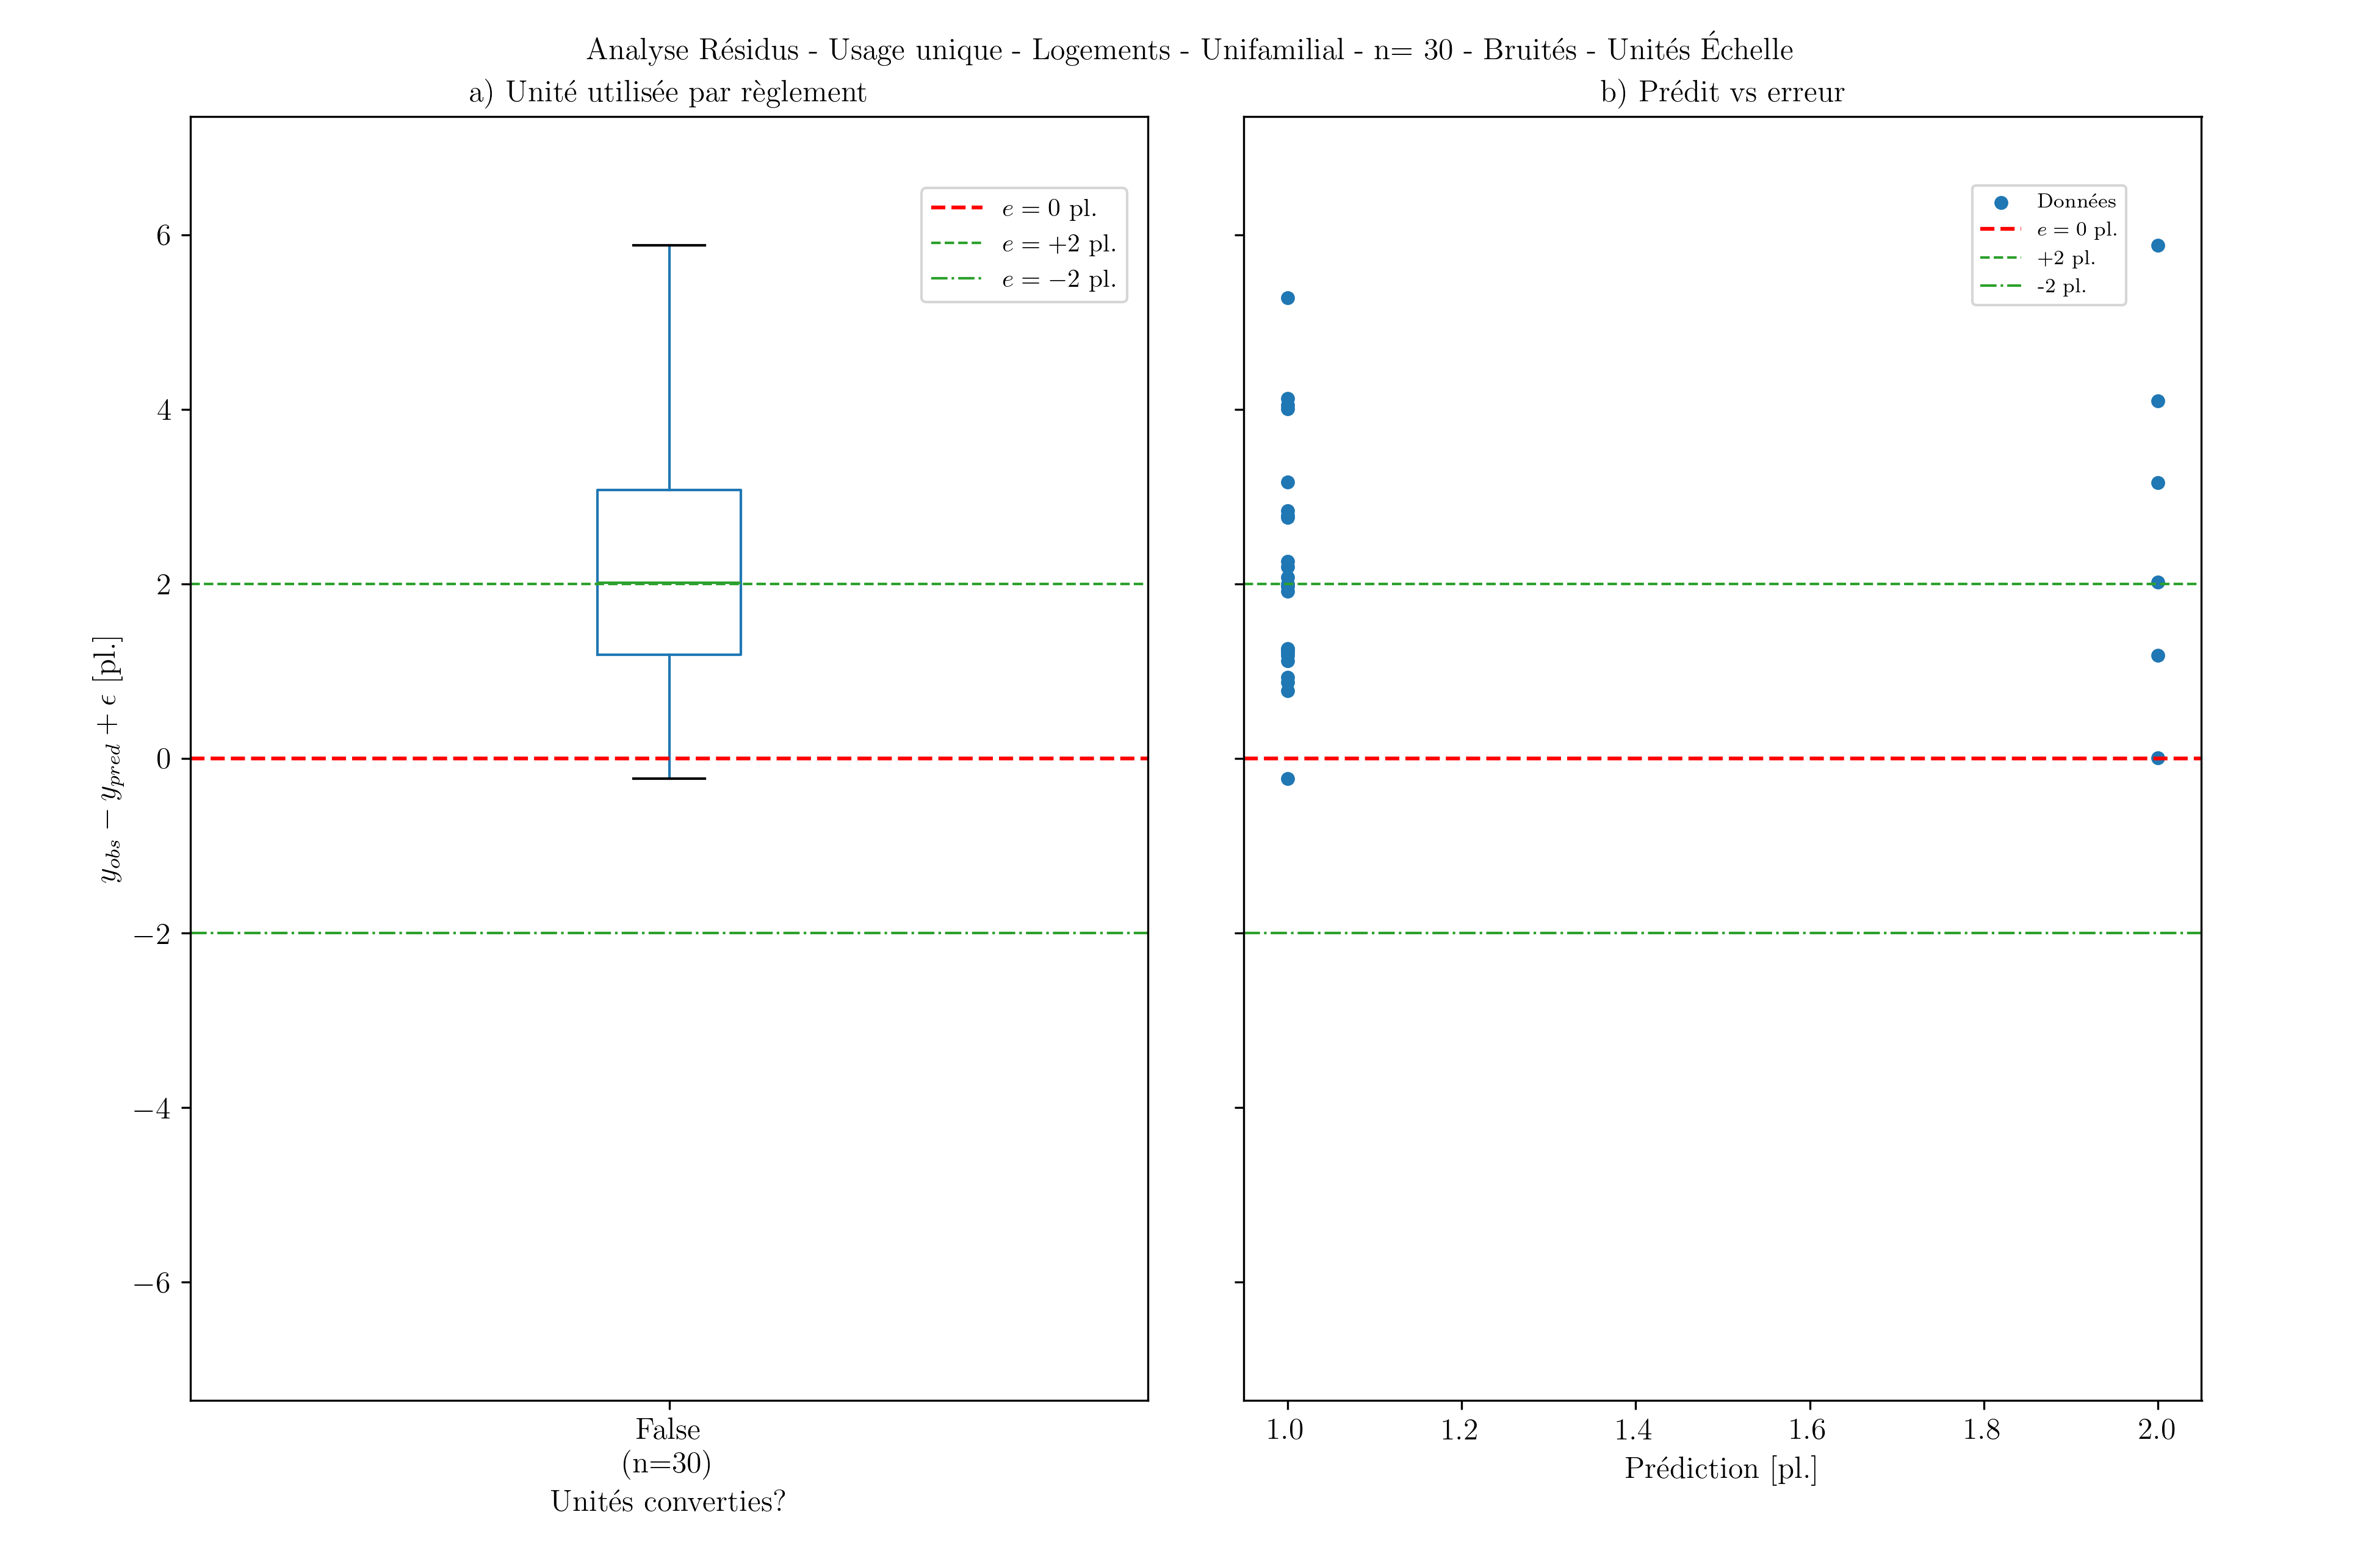
\includegraphics[width=1\linewidth]{images/ana_res_36_b_se_2_c.png}
        \caption{Analyse des résidus en fonction de la prédiction et des unités de formulation pour le logement unifamilial}
        \label{fig:ana-res-unit-pred-log-uni}
    \end{figure}
    \begin{figure}[H]
        \centering
        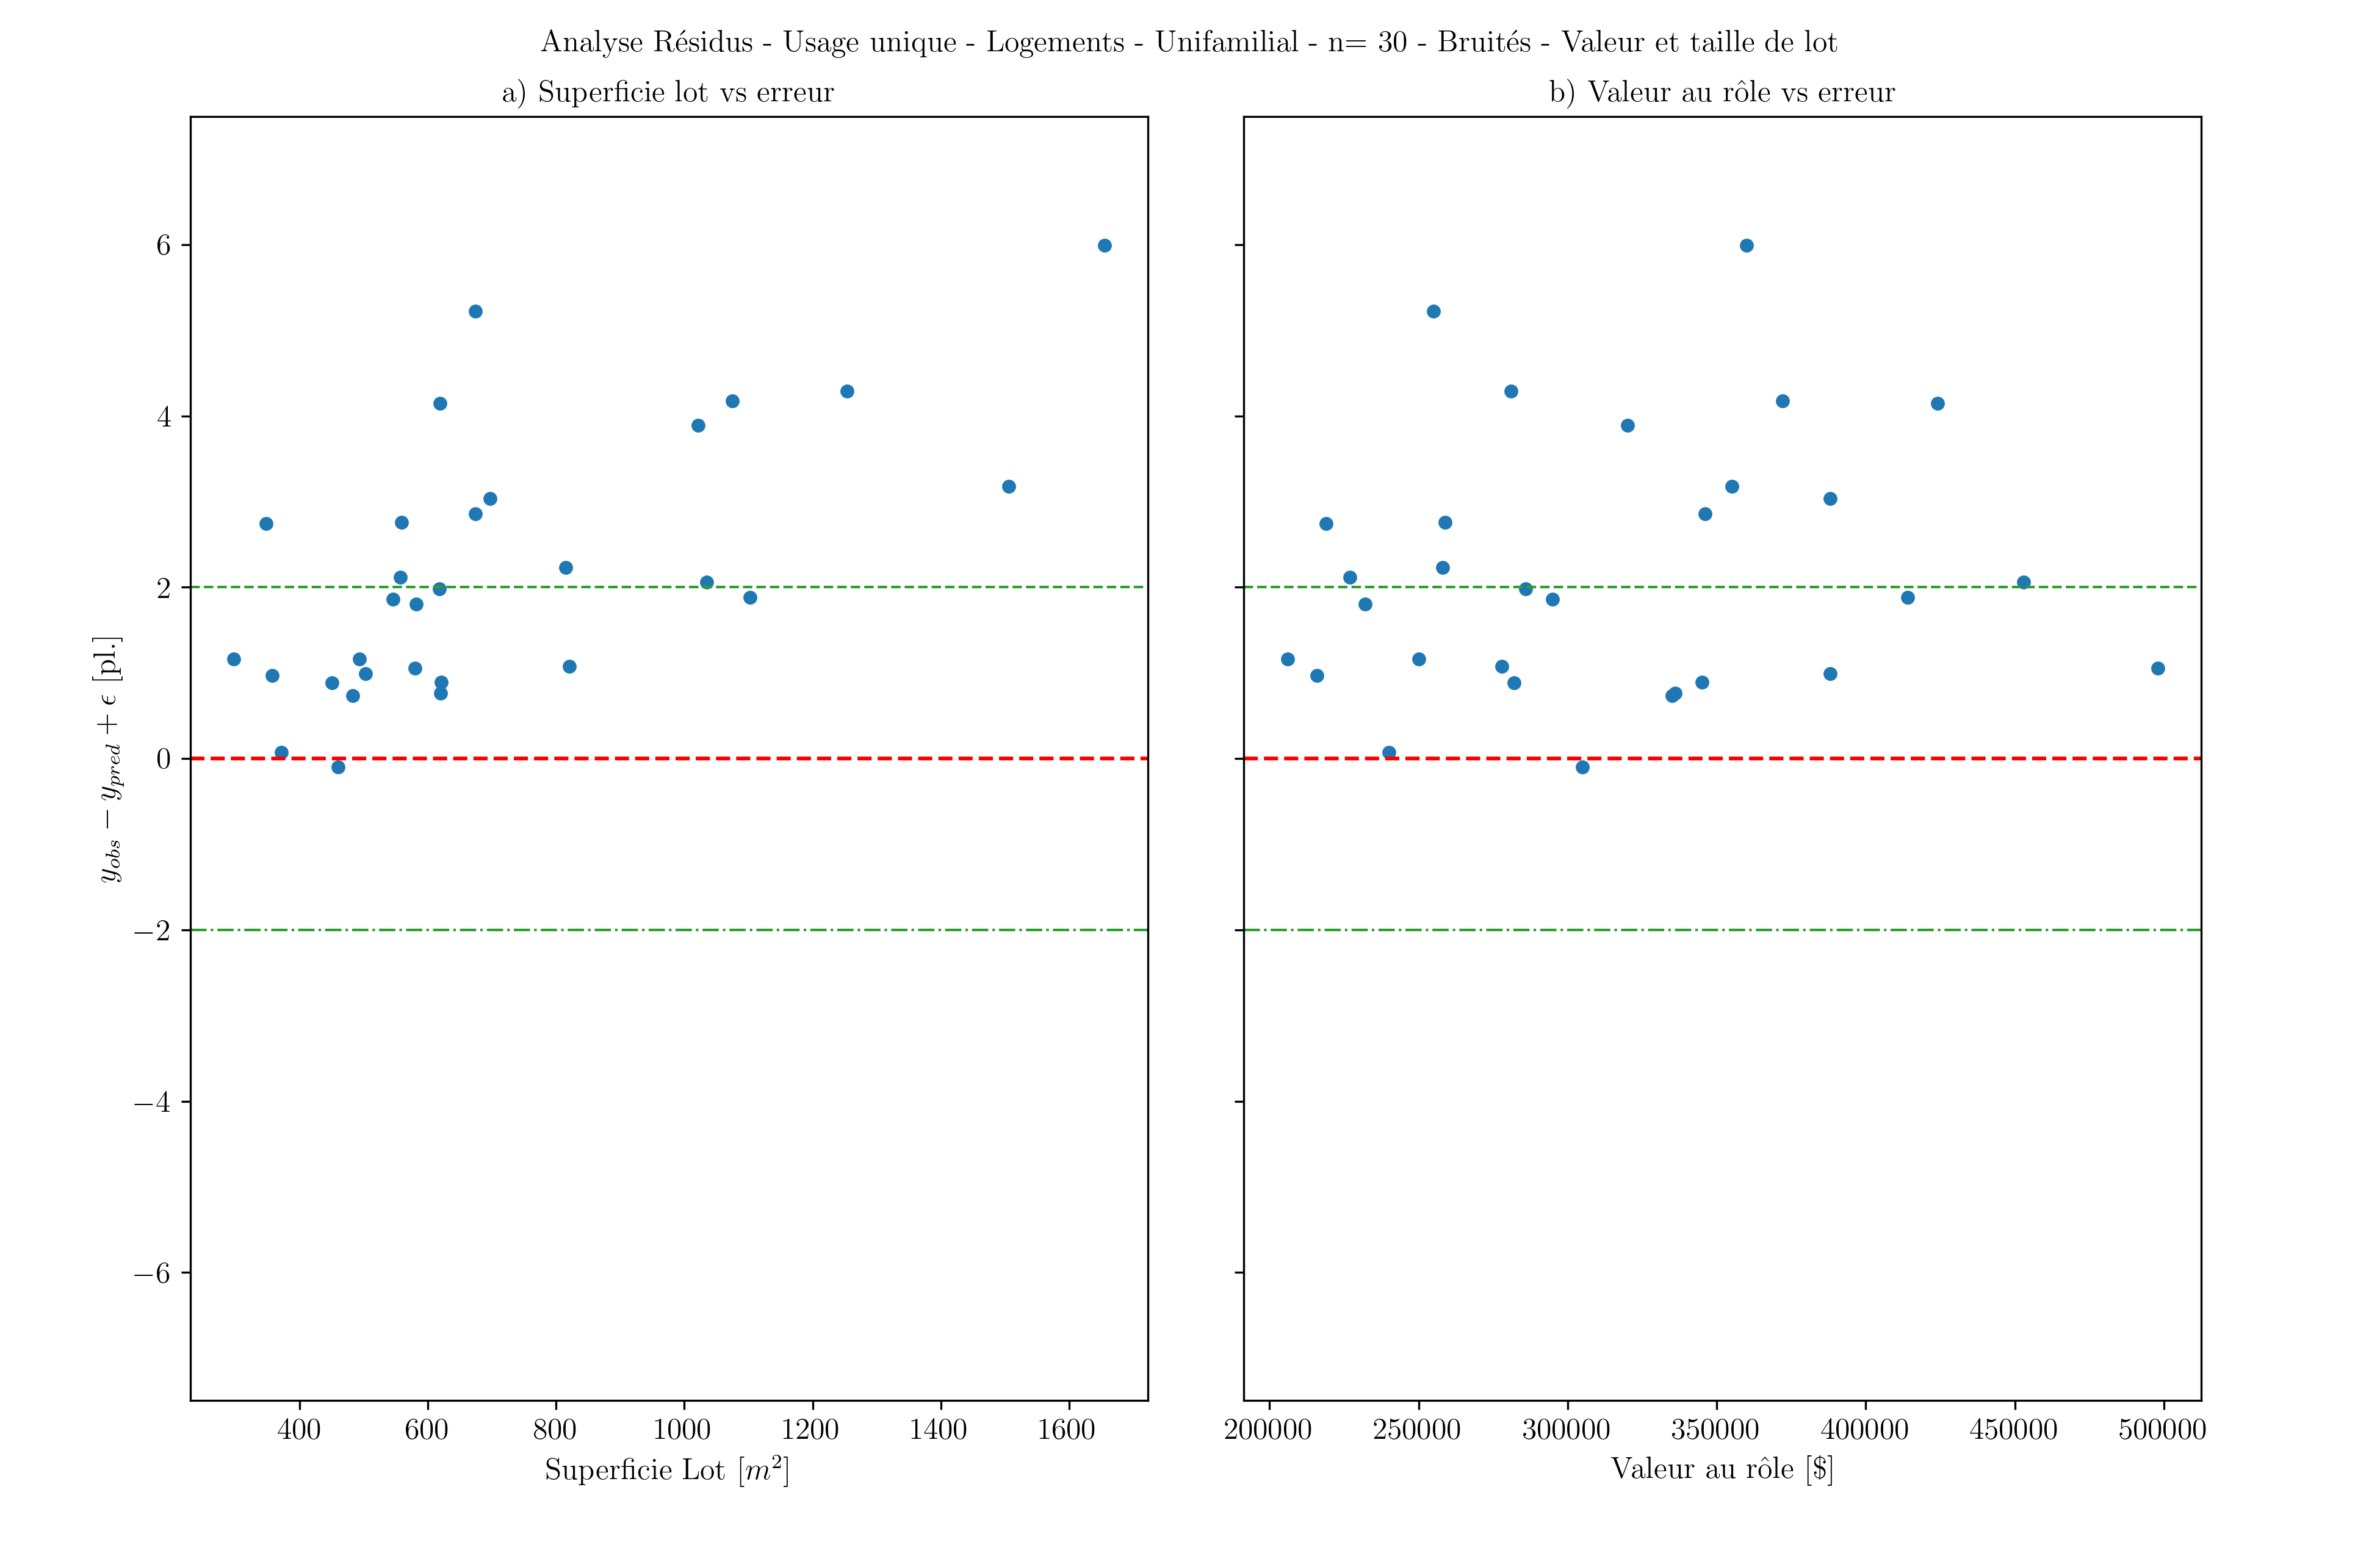
\includegraphics[width=1\linewidth]{images/ana_res_36_b_se_2_d.png}
        \caption{Analyse des résidus en fonction de la superficie du lot et de la valeur pour le logement unifamilial}
        \label{fig:ana-res-sup-val-log-uni}
    \end{figure}
    \begin{figure}[H]
        \centering
        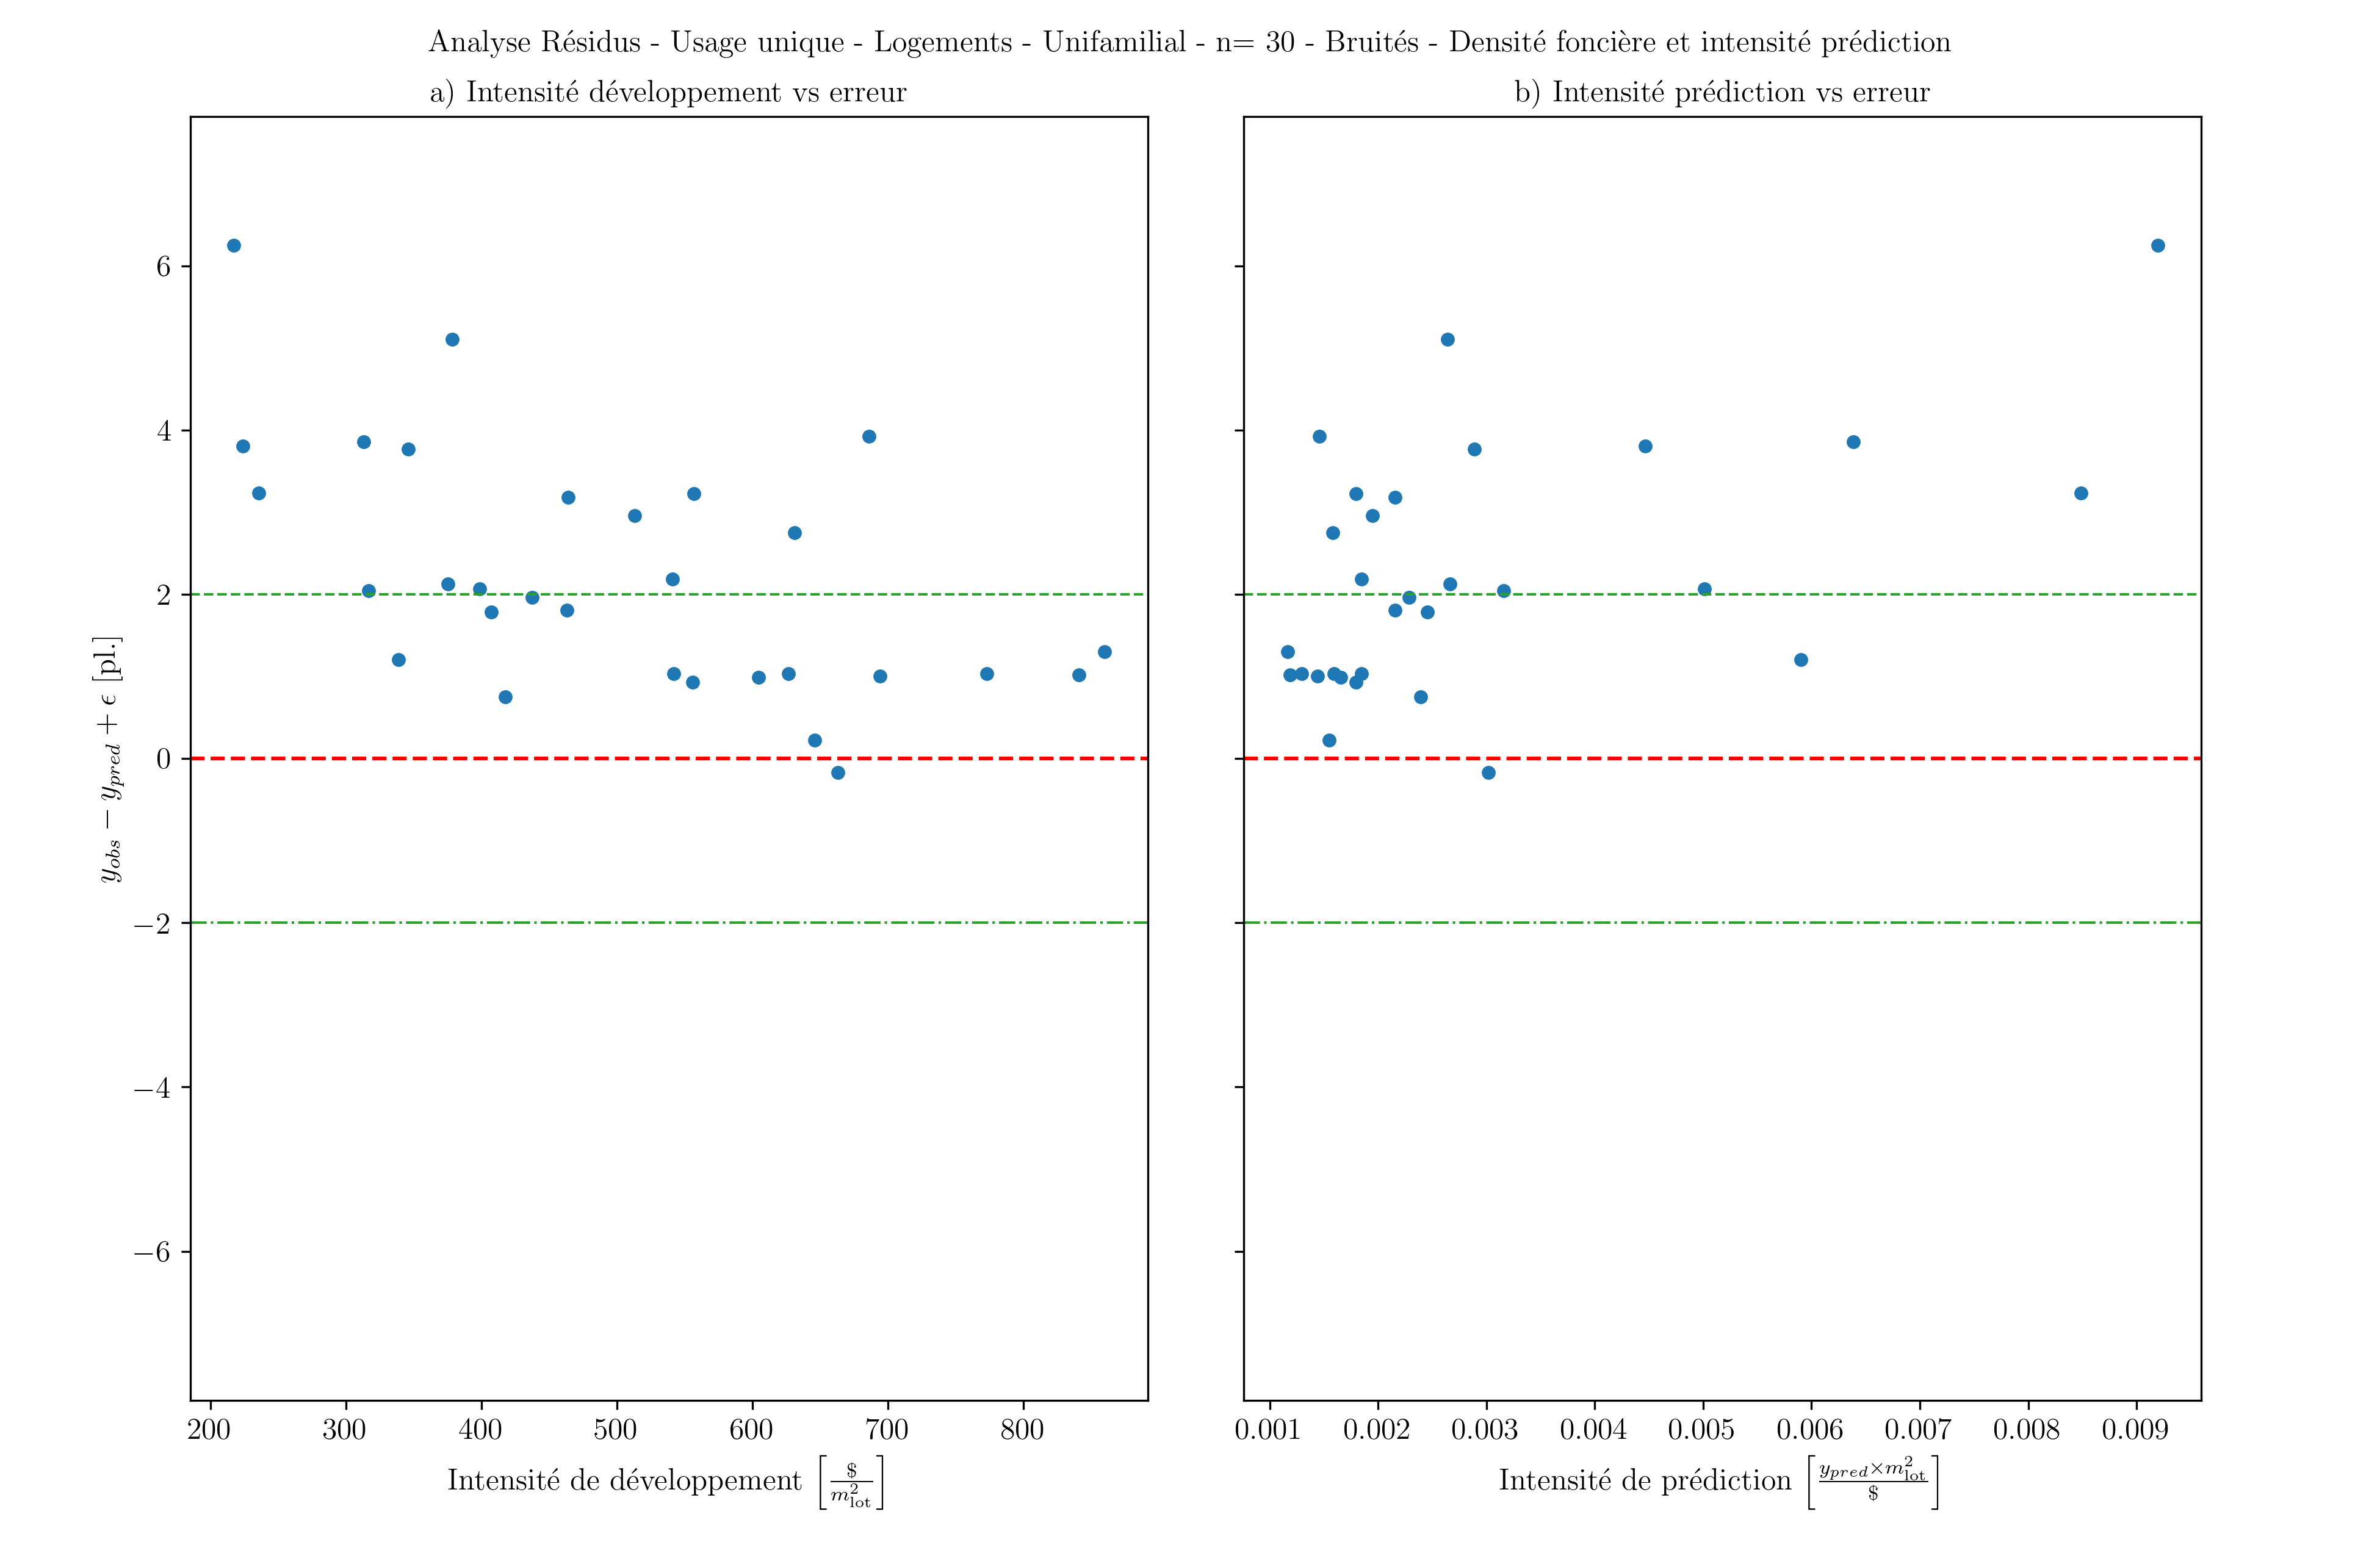
\includegraphics[width=1\linewidth]{images/ana_res_36_b_se_2_e.png}
        \caption{Analyse des résidus en fonction de l'intensité de développement et l'intensité de prédiction pour le logement unifamilial}
        \label{fig:ana-res-intens-log-uni}
    \end{figure}
\end{landscape}
\subsection{Résidentiel - 2 à 8 logements}
Trente lots contenant entre 2 et 8 logements ont été échantillonnés et comparés aux prédictions du modèle. Encore une fois, les données sont légèrement bruitées sur un intervalle $[-0.3,0.3]$ pour distinguer les points dans les graphiques XY. On constate dans ce cas-ci qu'il y a moins de biais systématiques puisque les moyennes des prédictions et des observations sont sensiblement les mêmes ($\bar{y}_{obs} = 4.33$ vs $\bar{y}_{pred} = 4.13$). Cependant, il existe encore une forte dispersion autour de la prédiction.\par
Une inspection visuelle de l'analyse des résidus indique que l'erreur varie avec la distance au parlement (fig.\ref{fig:ana-res-esp-temps-log-plex}b), la valeur au rôle par superficie du lot (fig. \ref{fig:ana-res-intens-log-plex}a) et potentiellement la date de construction (fig.\ref{fig:ana-res-esp-temps-log-plex}a). Les trois variables sont probablement corrélées entre elles. Généralement, plus l'échantillon est central, plus la valeur construite par superficie de lot est élevée, plus le modèle tend à surestimer la quantité de stationnements.
\begin{landscape}
    %\begin{figure}
    %    \centering
    %    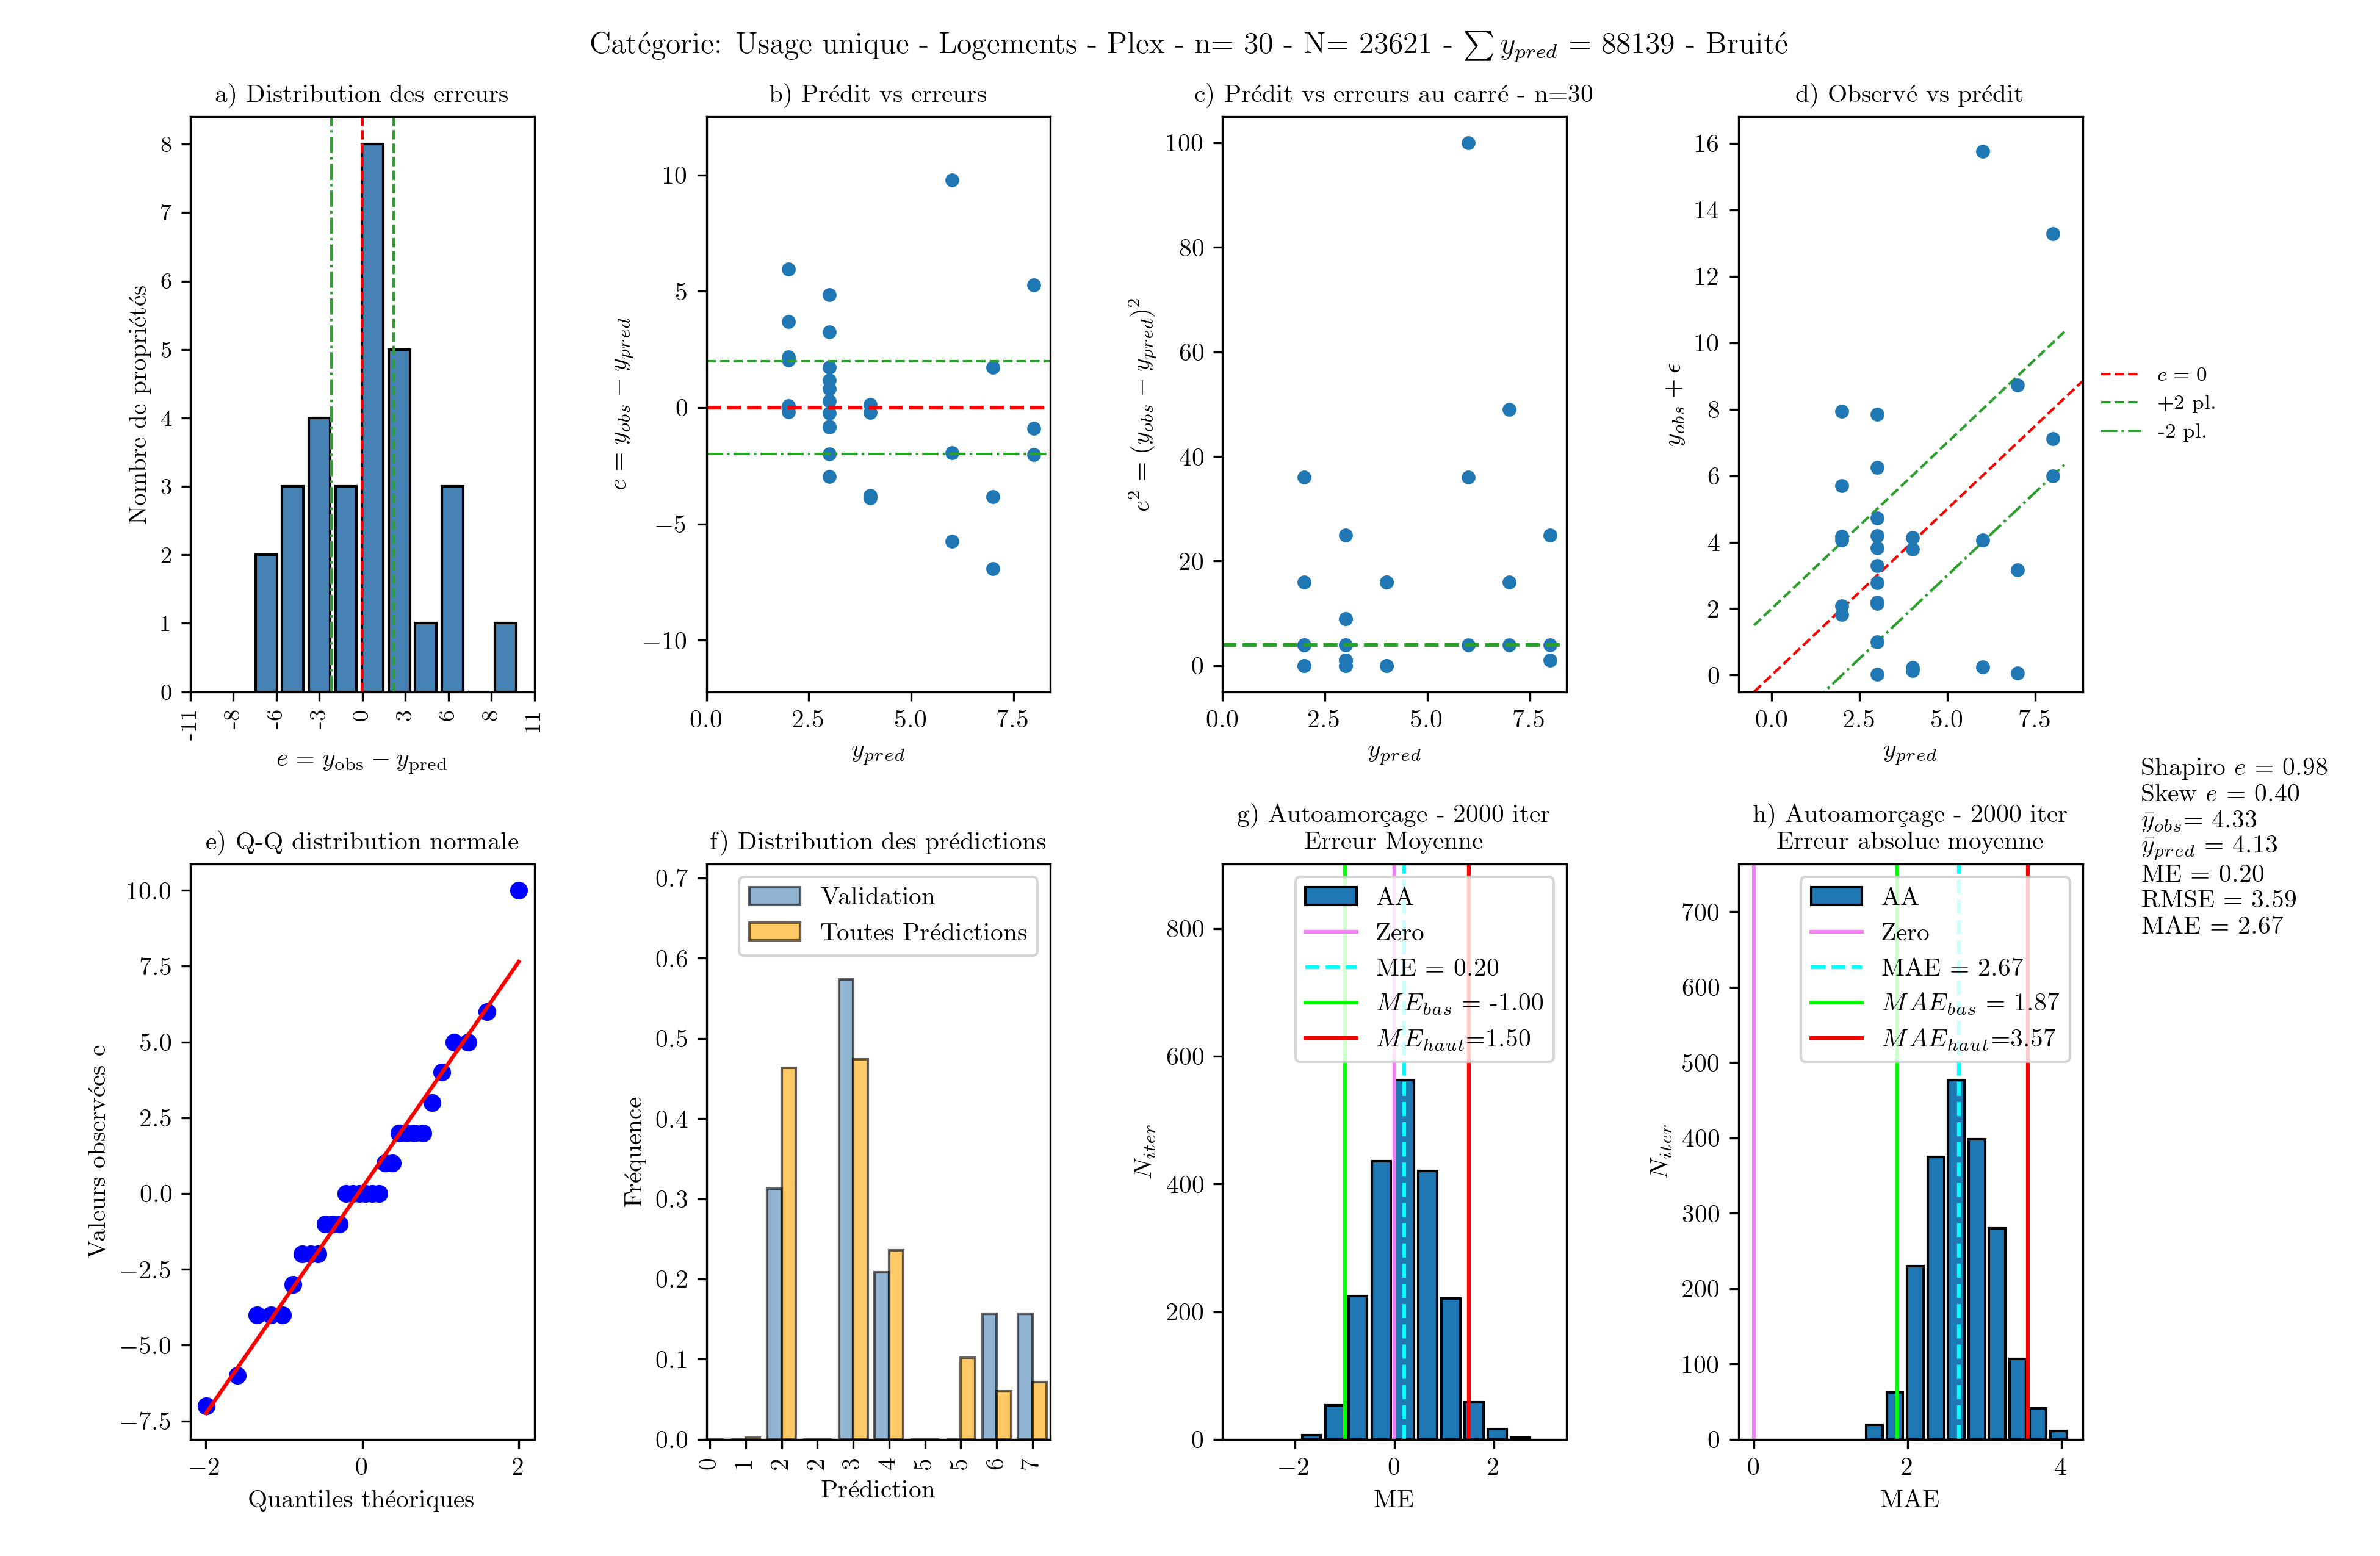
\includegraphics[scale=0.7]{images/int_erreur_43_b_se_2.png}
    %    \caption{Distribution et intervalles de prédiction d'erreur pour les lots avec 2 à 8 logements}
    %    \label{fig:intervals-dist-val-log-plex}
    %\end{figure}
    \begin{figure}[H]
        \centering
        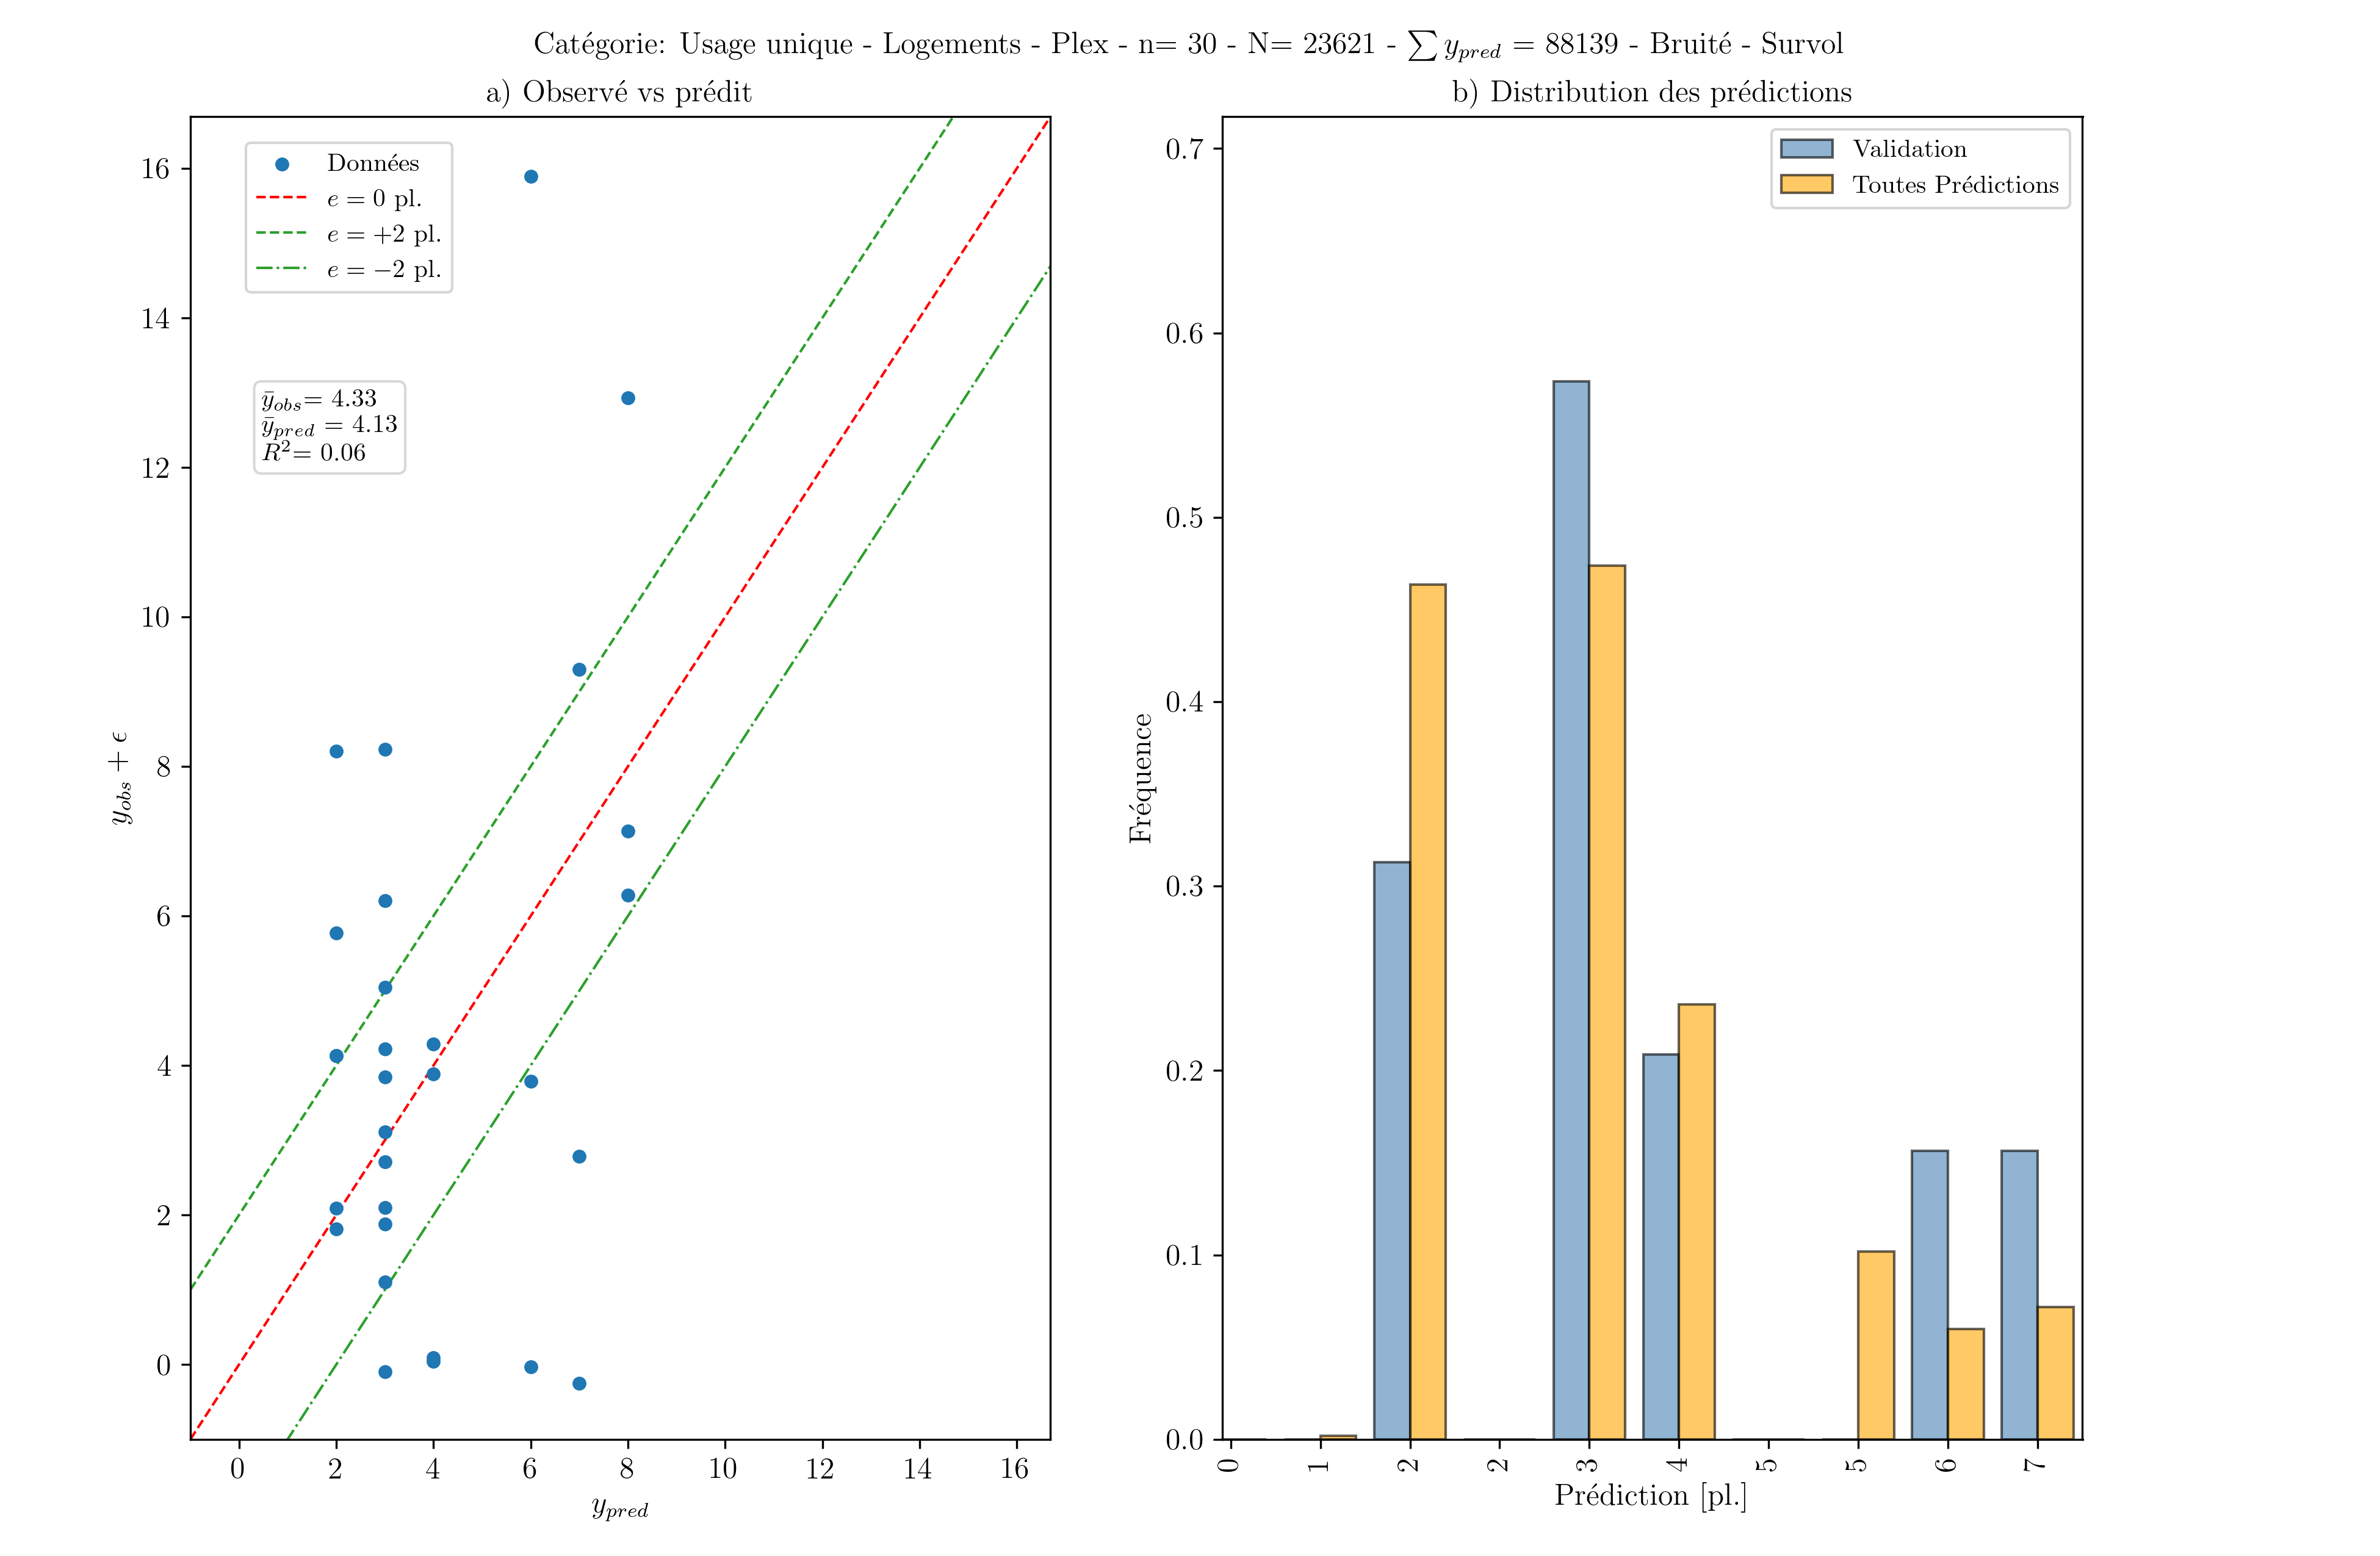
\includegraphics[width=1\linewidth]{images/int_erreur_43_b_se_2_a.png}
        \caption{Distribution des prédictions pour les lots avec 2 à 8 logements}
        \label{fig:int-dist-pred-log-plex}
    \end{figure}
    \begin{figure}[H]
        \centering
        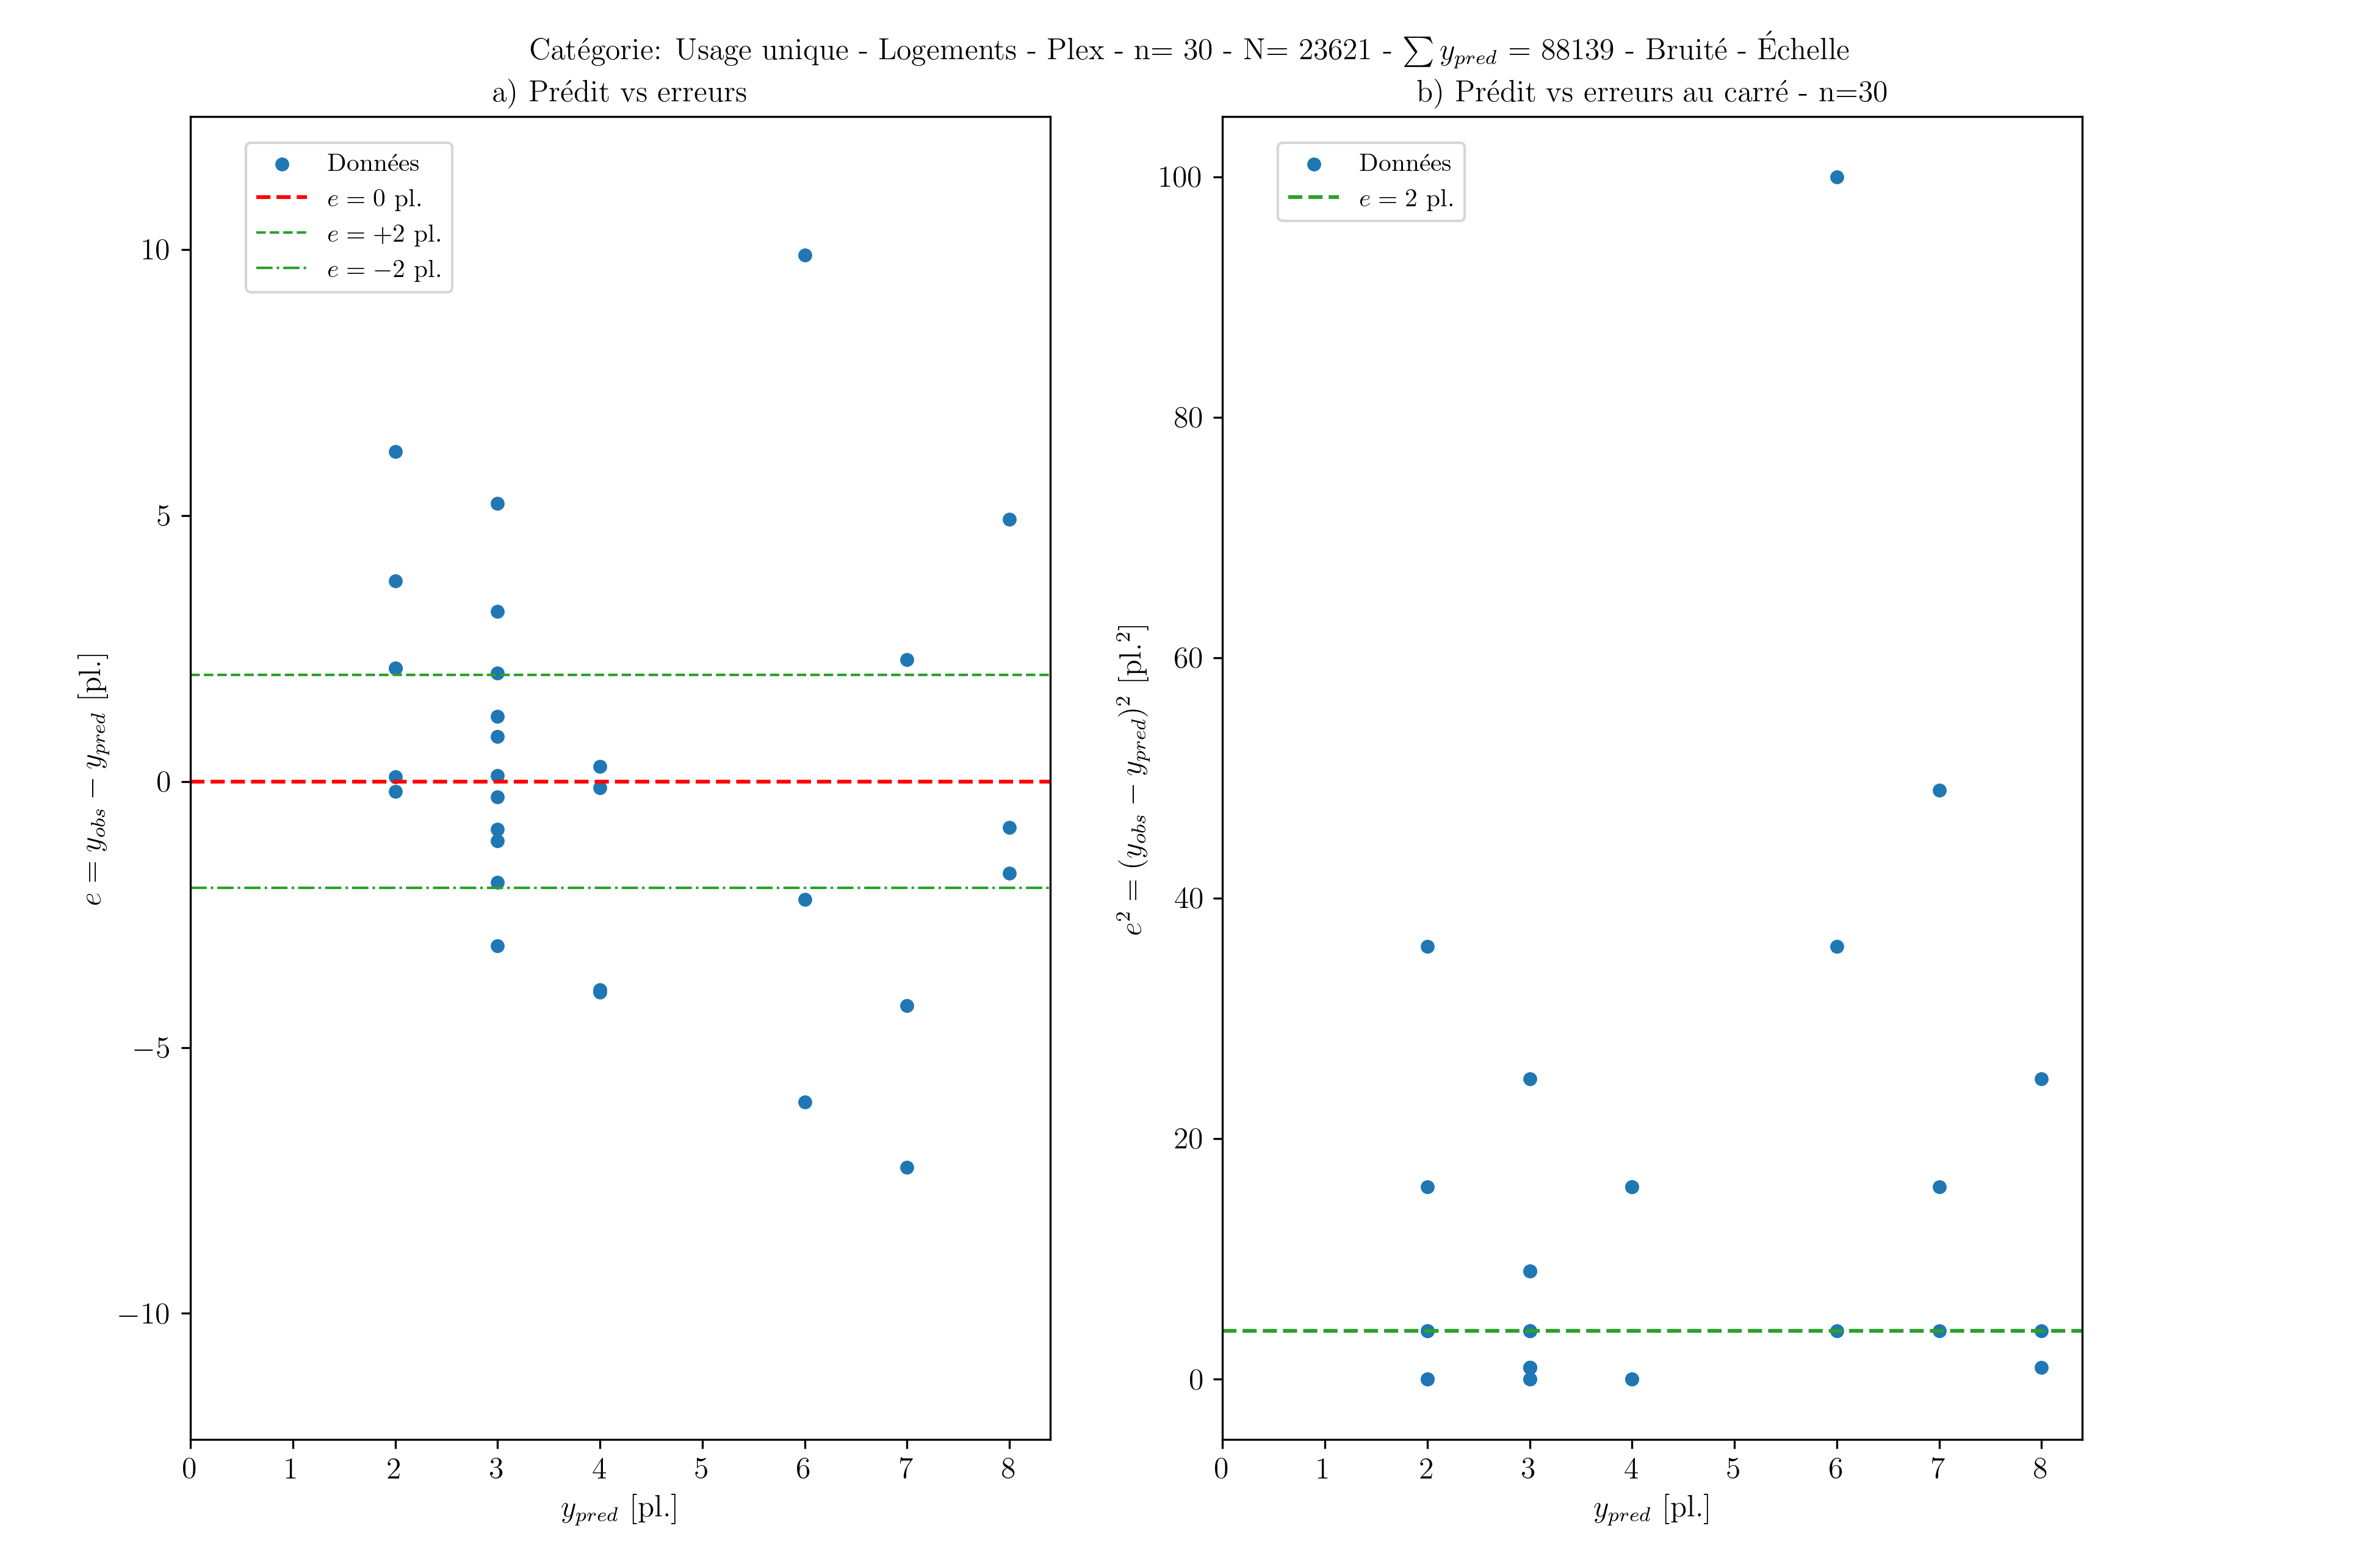
\includegraphics[width=1\linewidth]{images/int_erreur_43_b_se_2_b.png}
        \caption{Erreur en fonction des prédictions pour les lots avec 2 à 8 logements}
        \label{fig:err-err-quad-pred-log-plex}
    \end{figure}
    \begin{figure}[H]
        \centering
        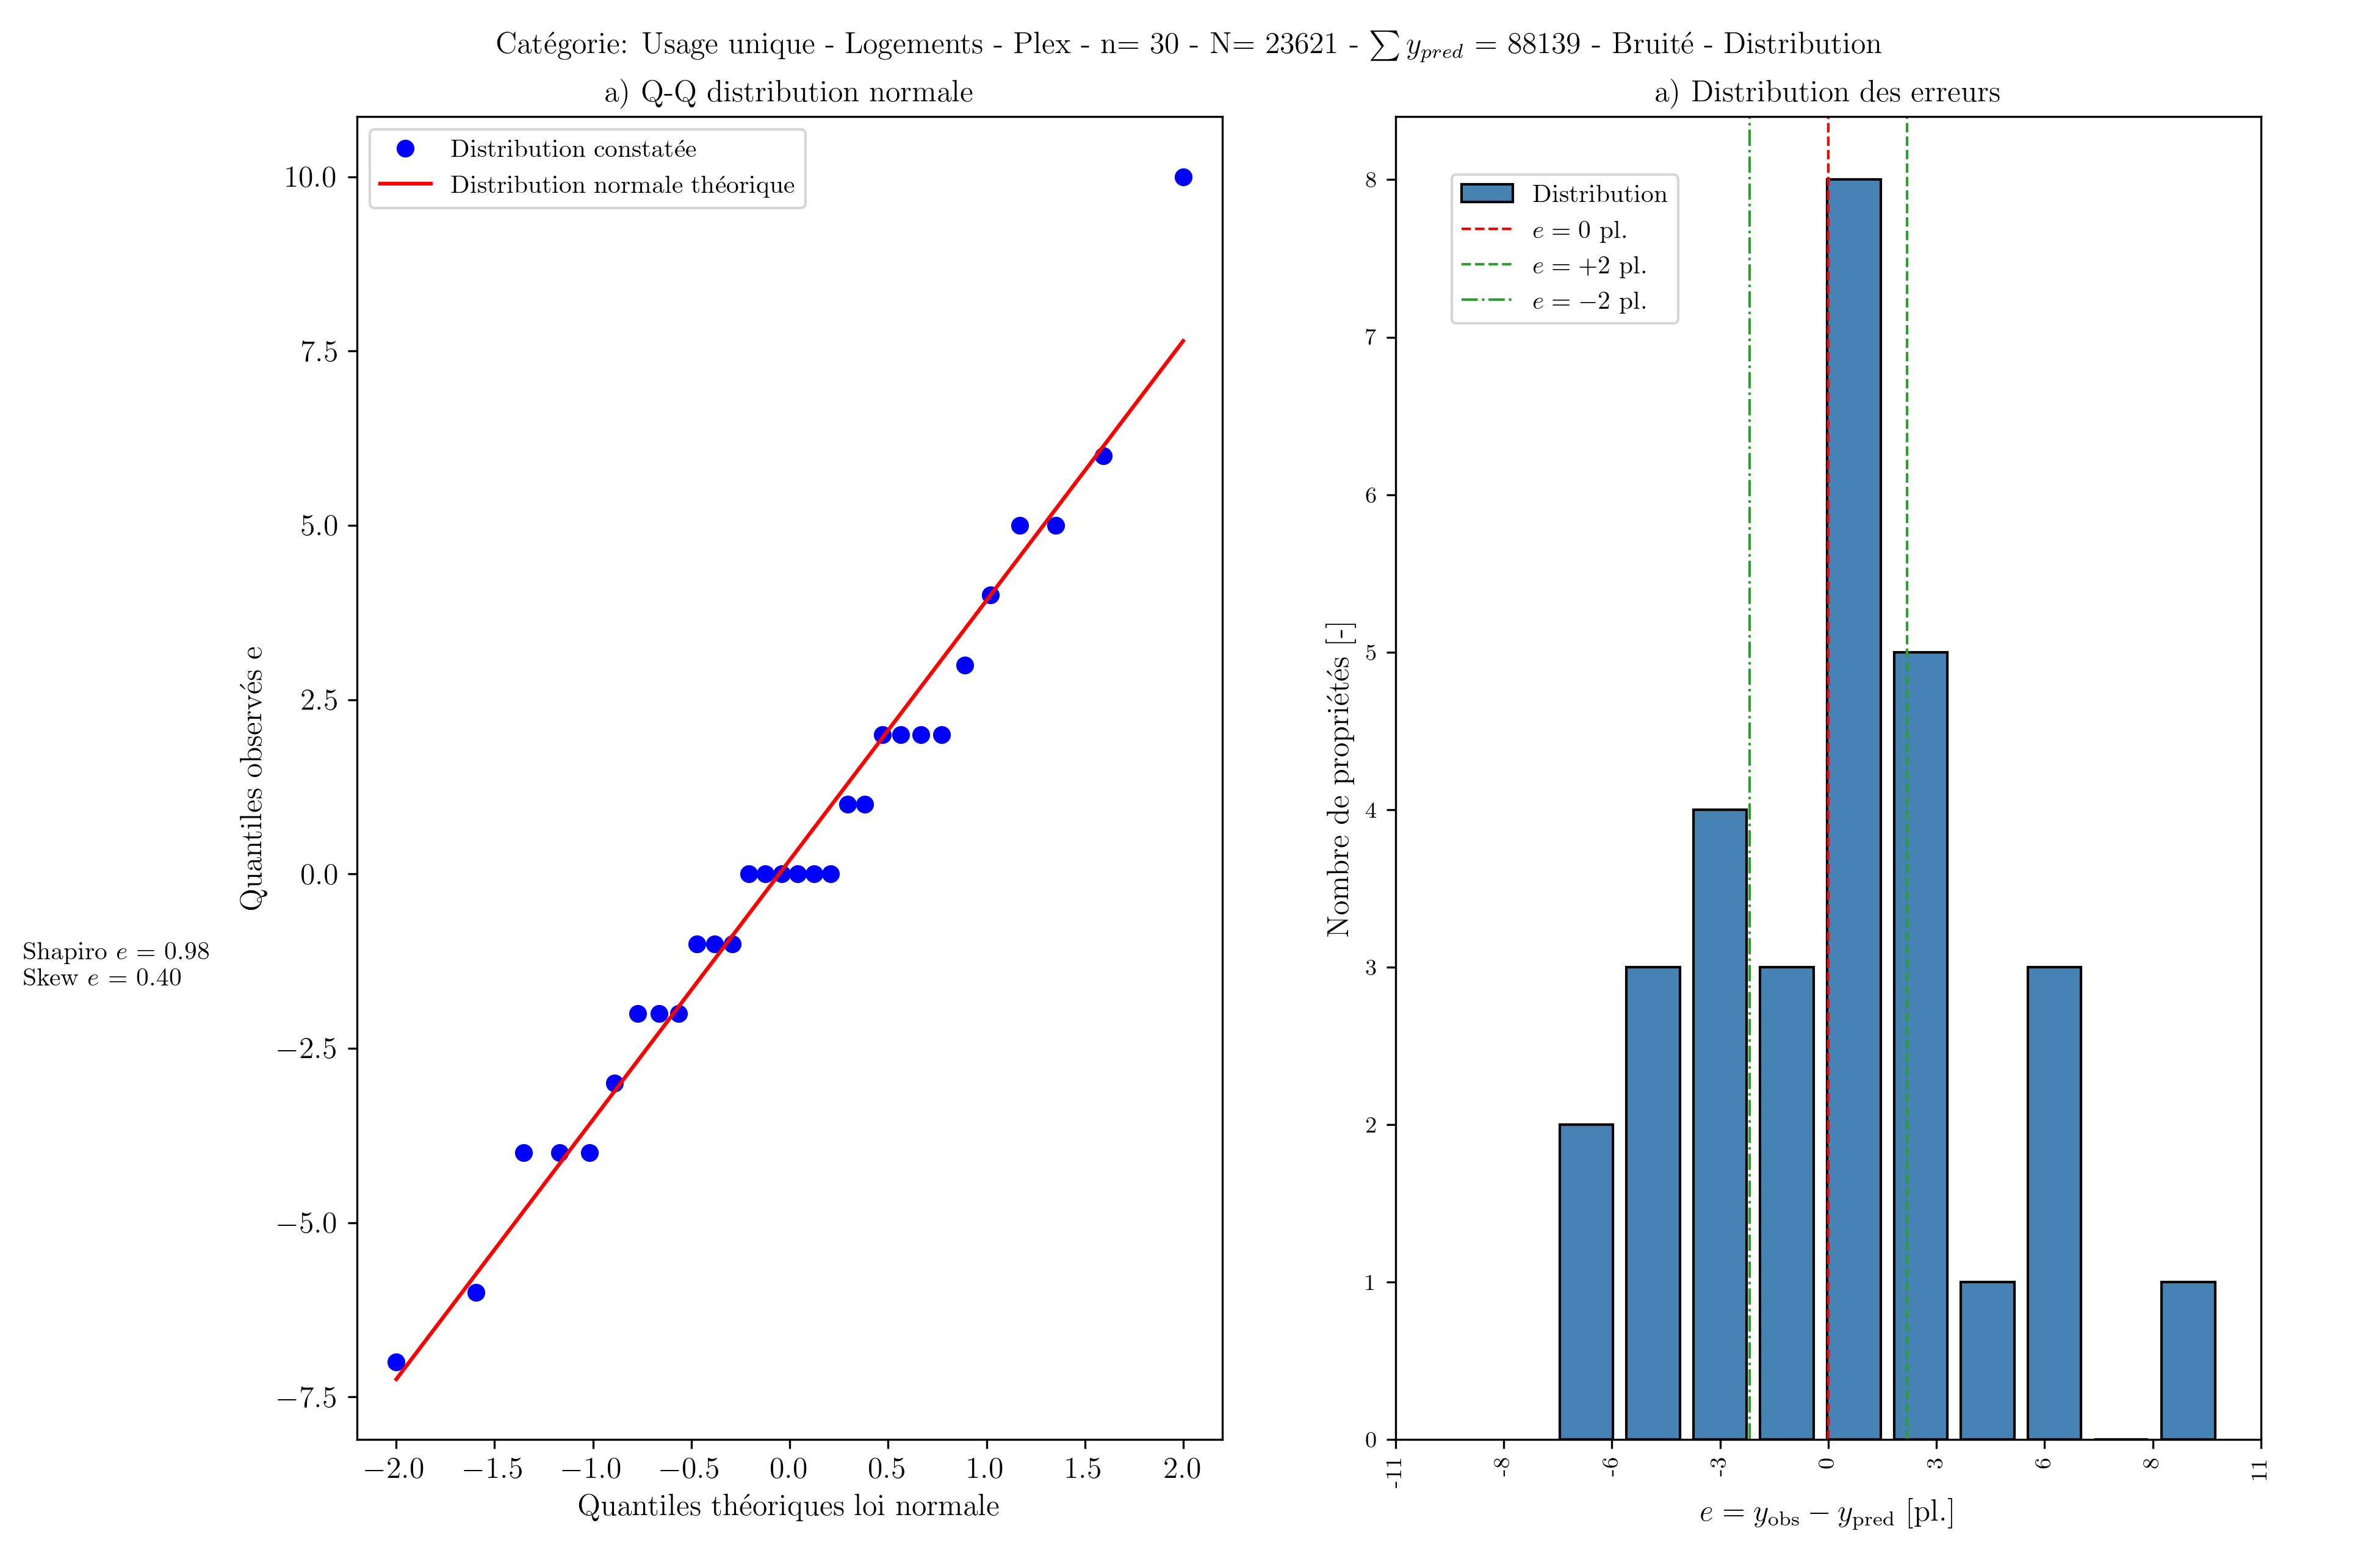
\includegraphics[width=1\linewidth]{images/int_erreur_43_b_se_2_c.png}
        \caption{Distribution et normalité des erreurs pour les lots avec 2 à 8 logements}
        \label{fig:dist-erreur-norm-log-plex}
    \end{figure}
    \begin{figure}[H]
        \centering
        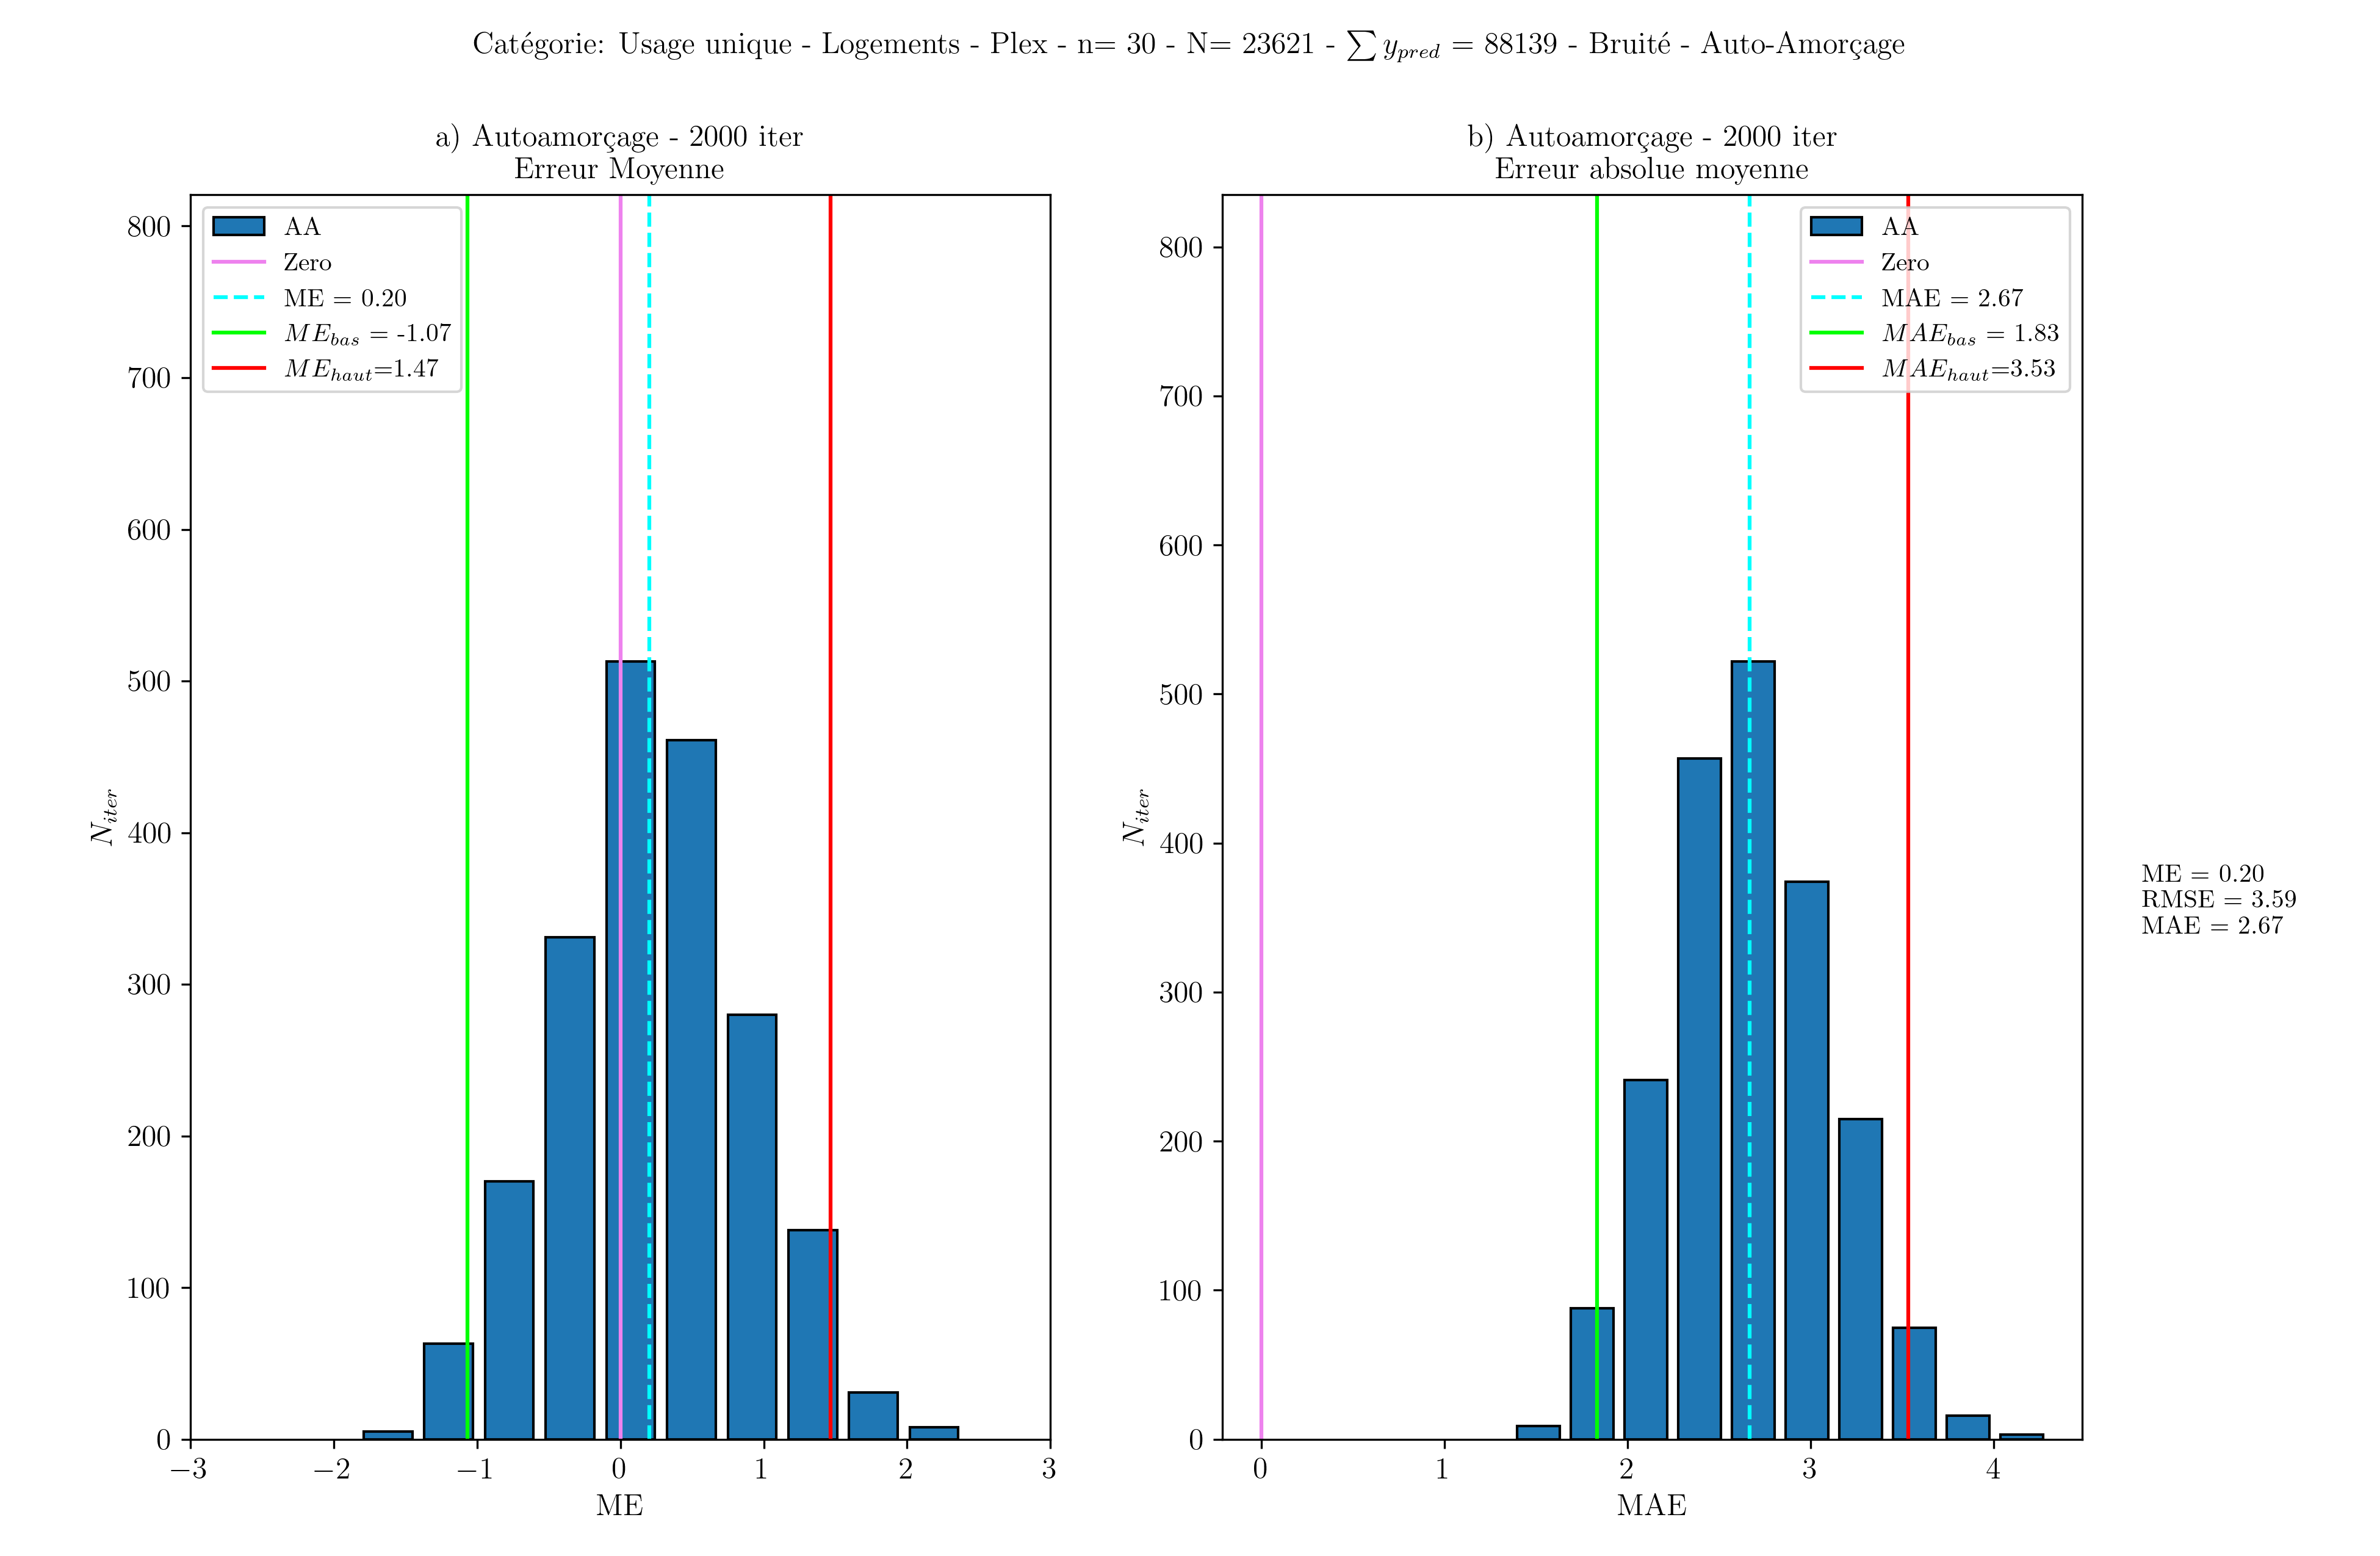
\includegraphics[width=1\linewidth]{images/int_erreur_43_b_se_2_d.png}
        \caption{Distribution des métriques d'erreur après auto-amorçage pour les lots avec 2 à 8 logements}
        \label{fig:auto-amor-log-plex}
    \end{figure}
    %\begin{figure}
    %    \centering
    %    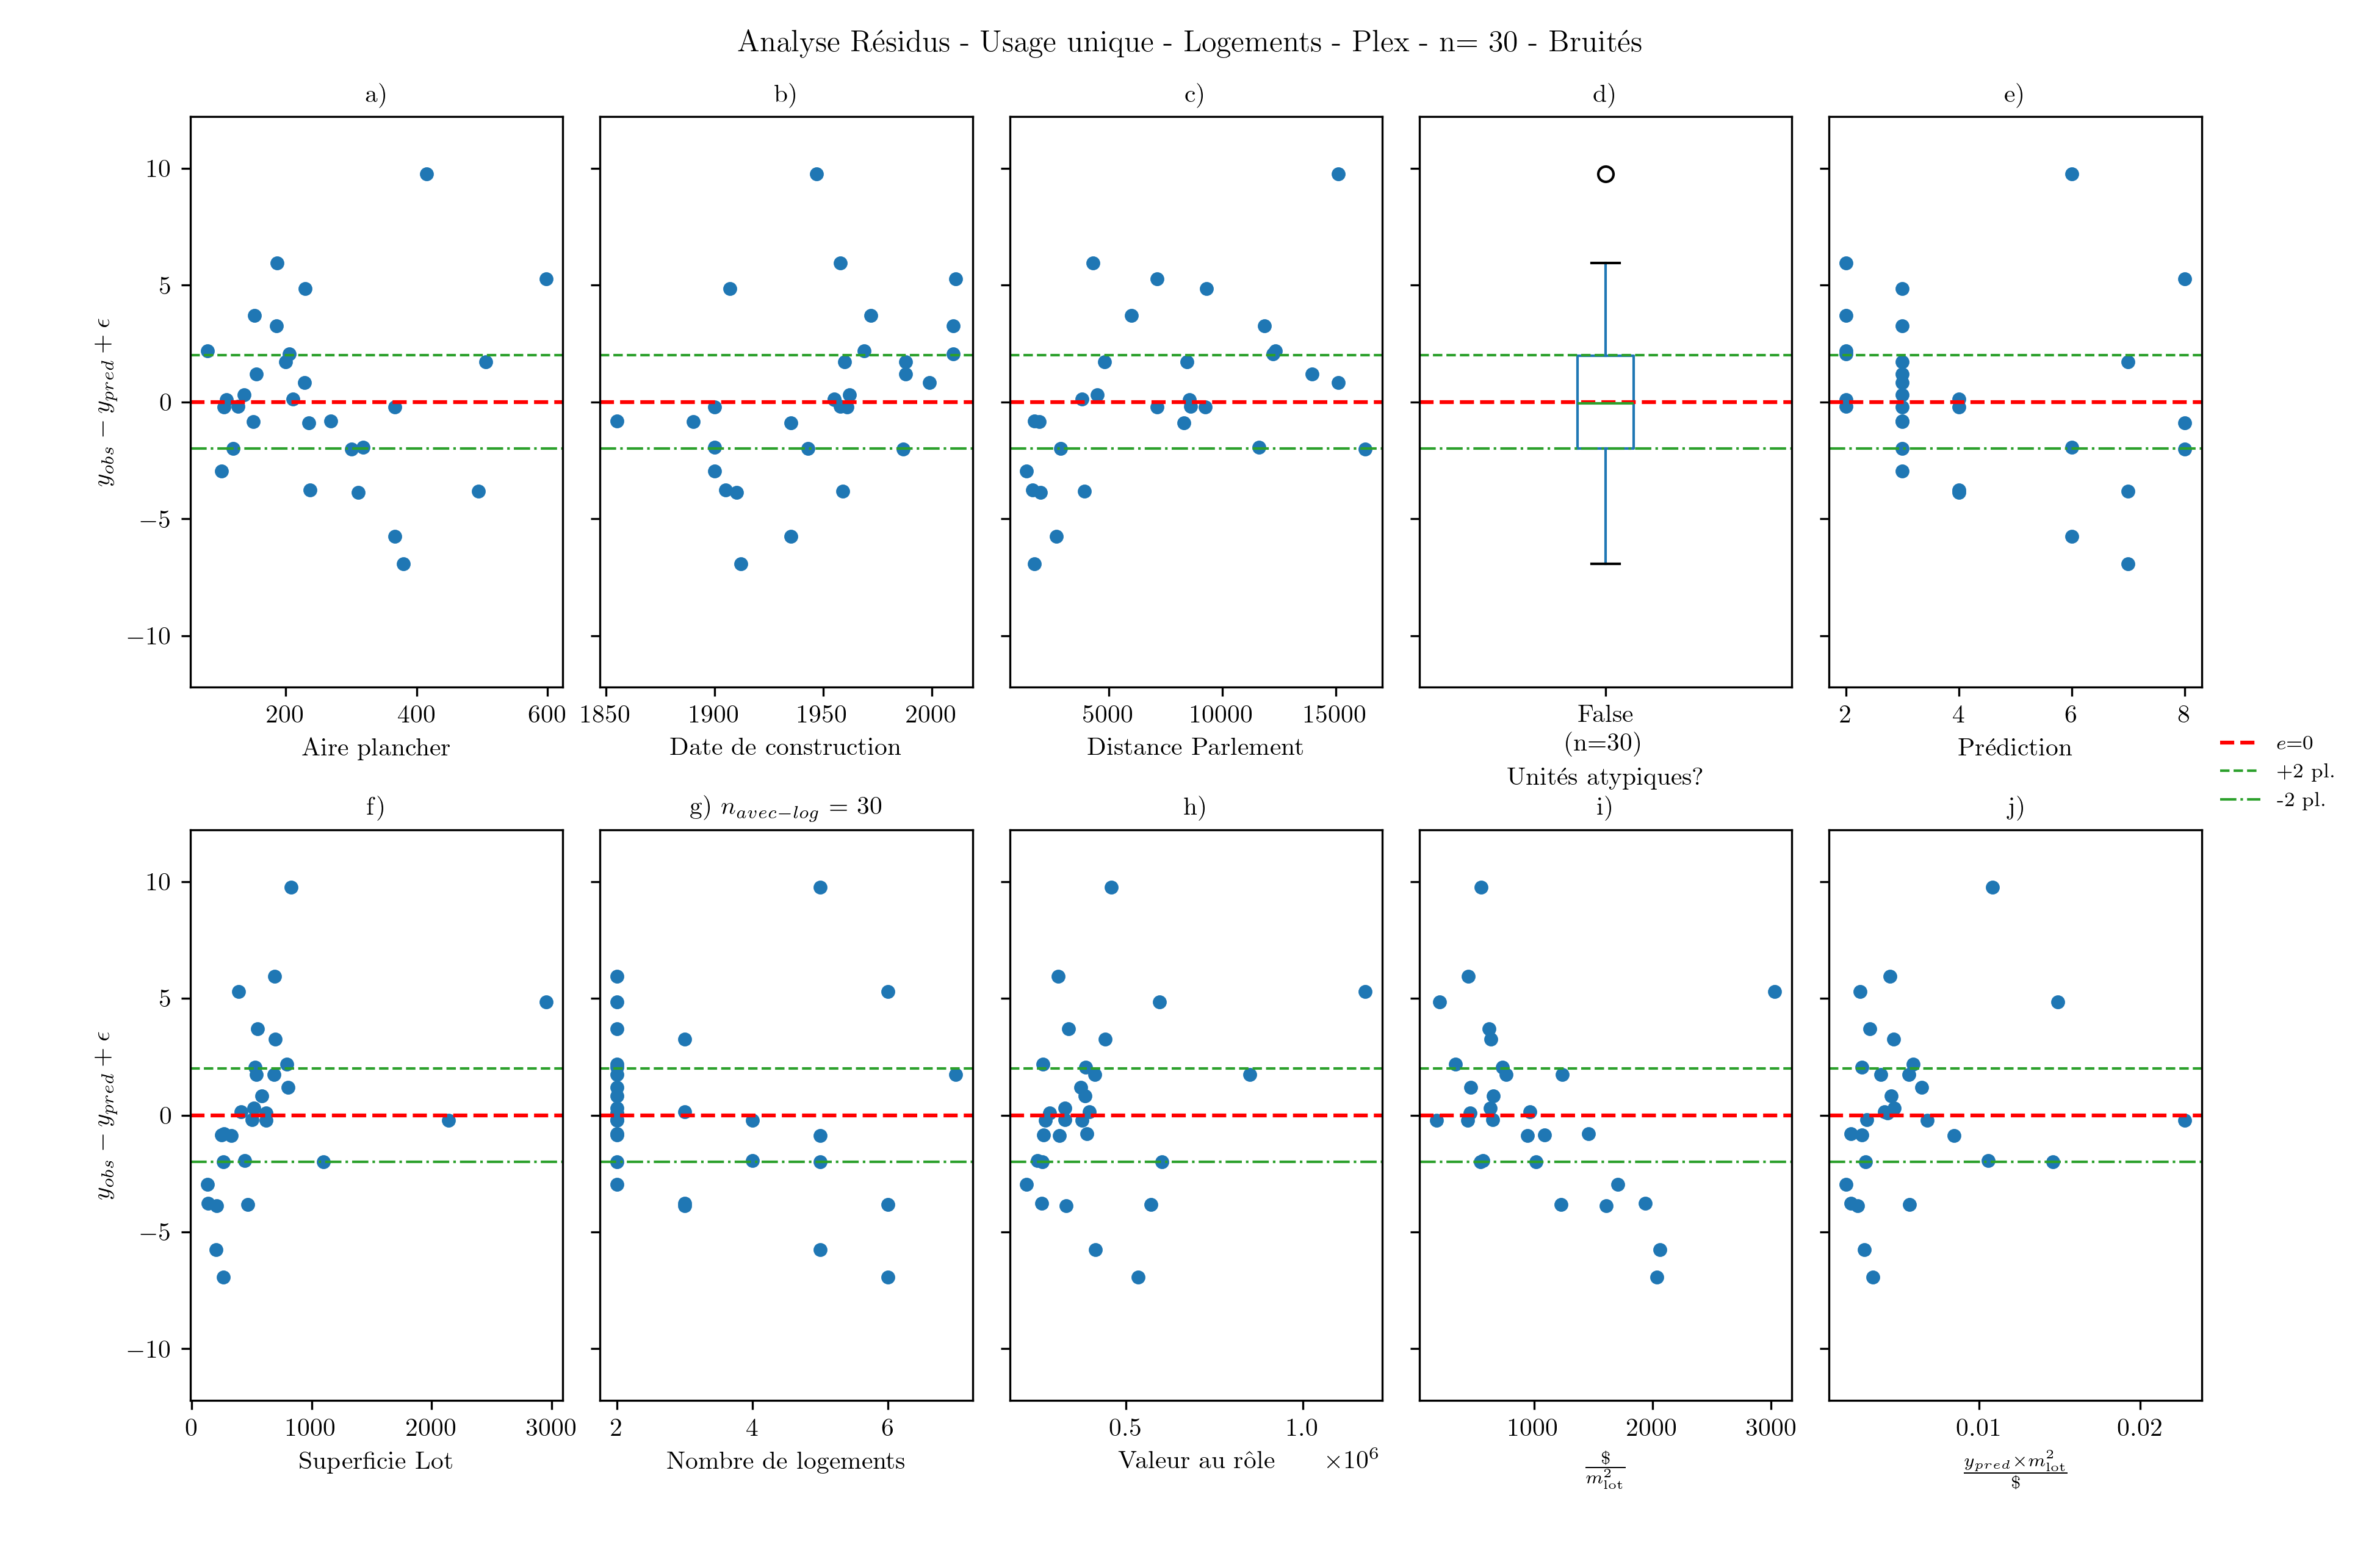
\includegraphics[scale=0.7]{images/ana_res_43_b_se_2.png}
    %    \caption{Analyse des résidus de la prédiction pour les lots avec 2 à 8 logements}
    %    \label{fig:ana-residu-log-plex}
    %\end{figure}
    \begin{figure}[H]
        \centering
        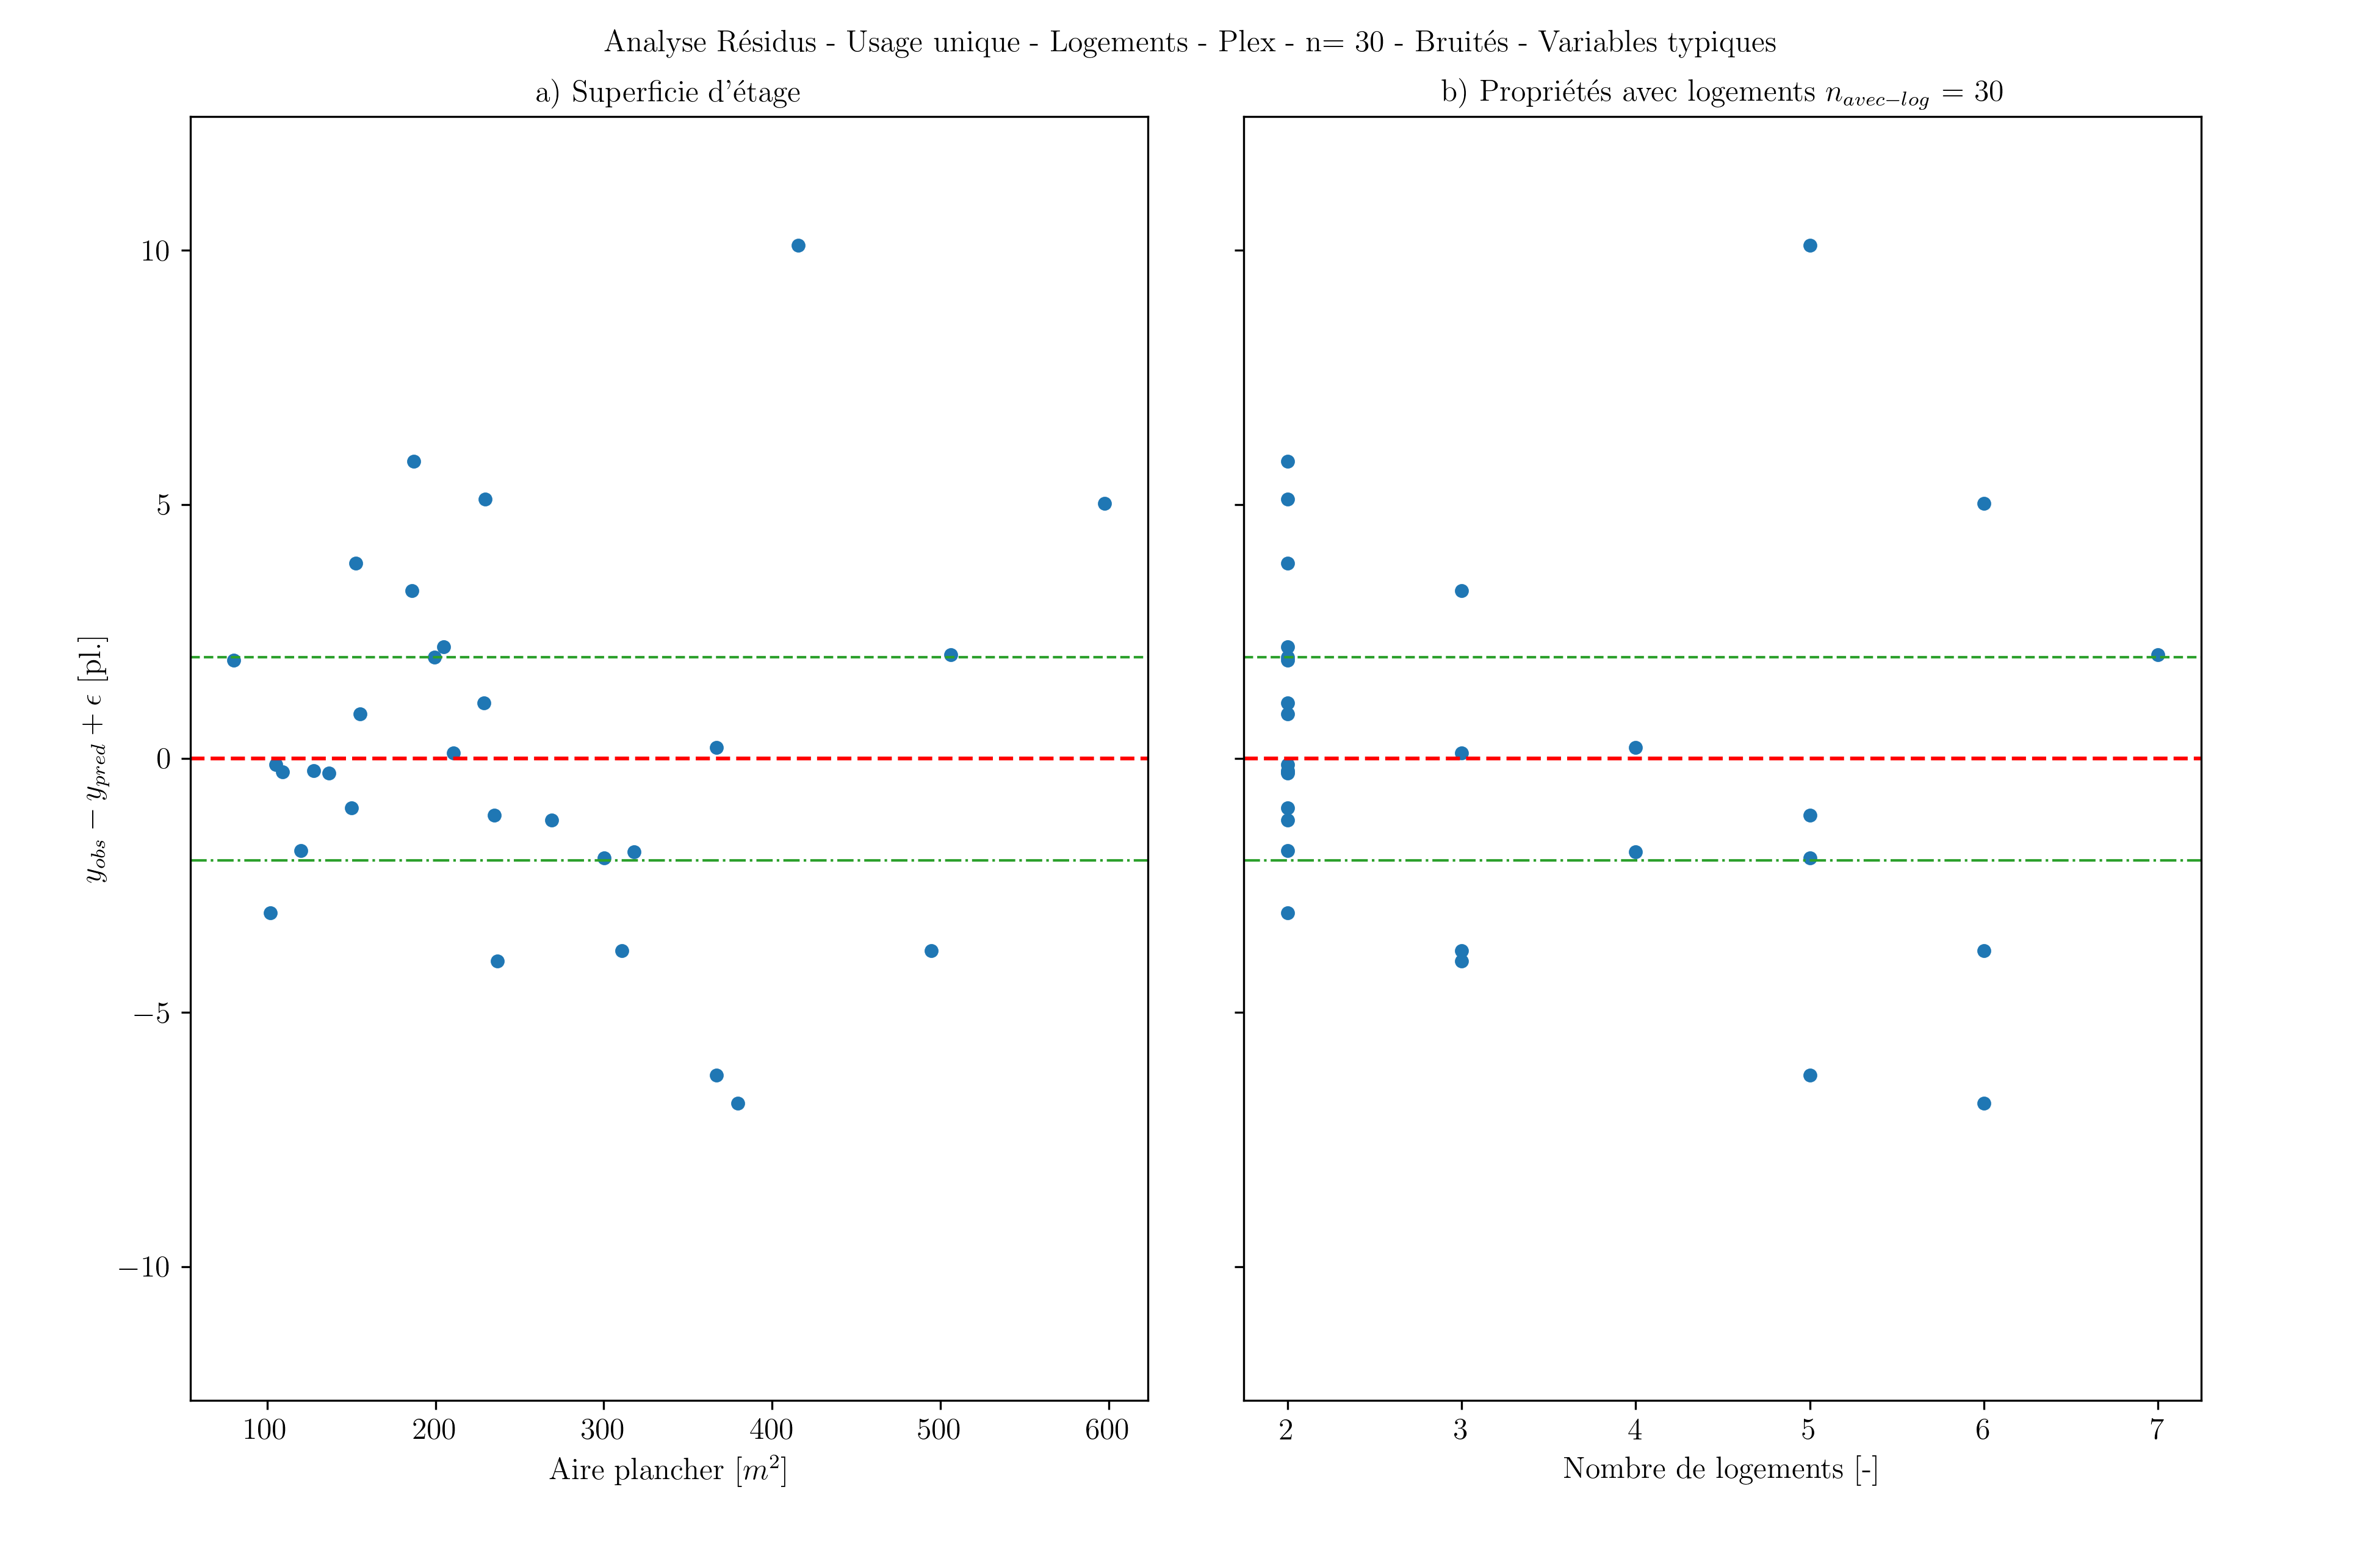
\includegraphics[width=1\linewidth]{images/ana_res_43_b_se_2_a.png}
        \caption{Analyse des résidus en fonction des propriétés de construction pour les lots avec 2 à 8 logements}
        \label{fig:ana-res-prop-phys-log-plex}
    \end{figure}
    \begin{figure}[H]
        \centering
        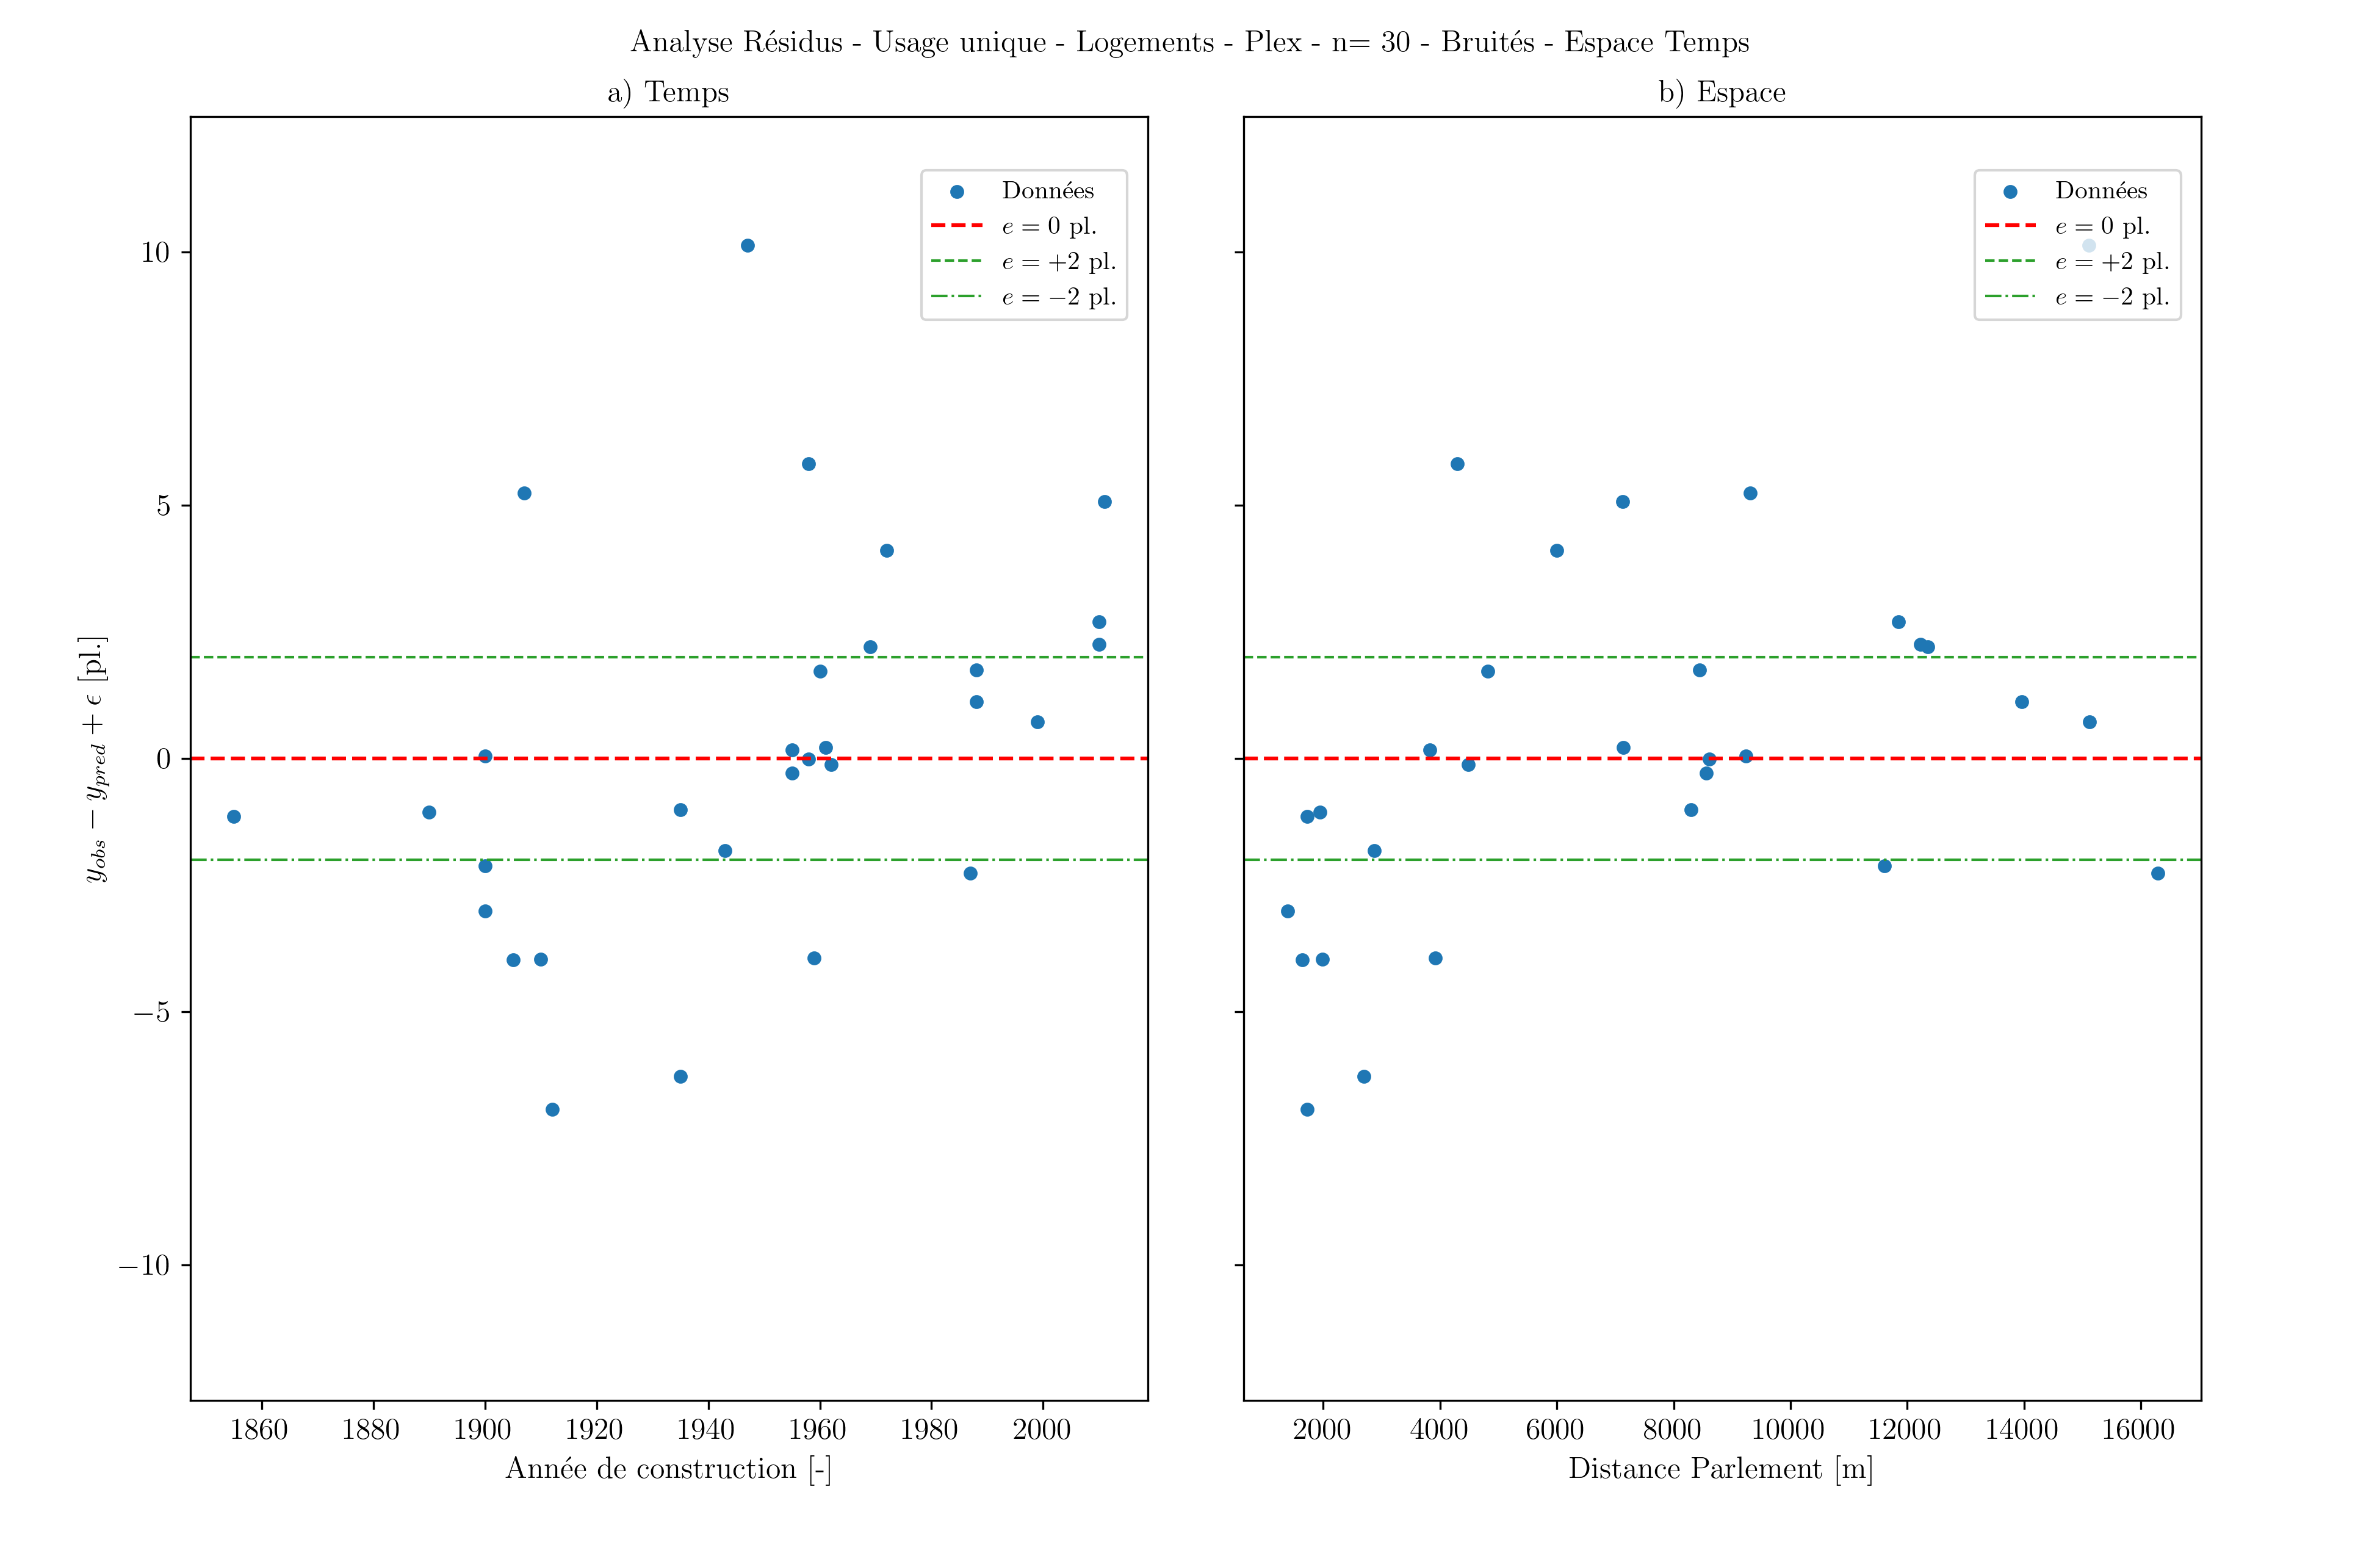
\includegraphics[width=1\linewidth]{images/ana_res_43_b_se_2_b.png}
        \caption{Analyse des résidus en fonction de l'espace et de l'année de construction pour les lots avec 2 à 8 logements}
        \label{fig:ana-res-esp-temps-log-plex}
    \end{figure}
    \begin{figure}[H]
        \centering
        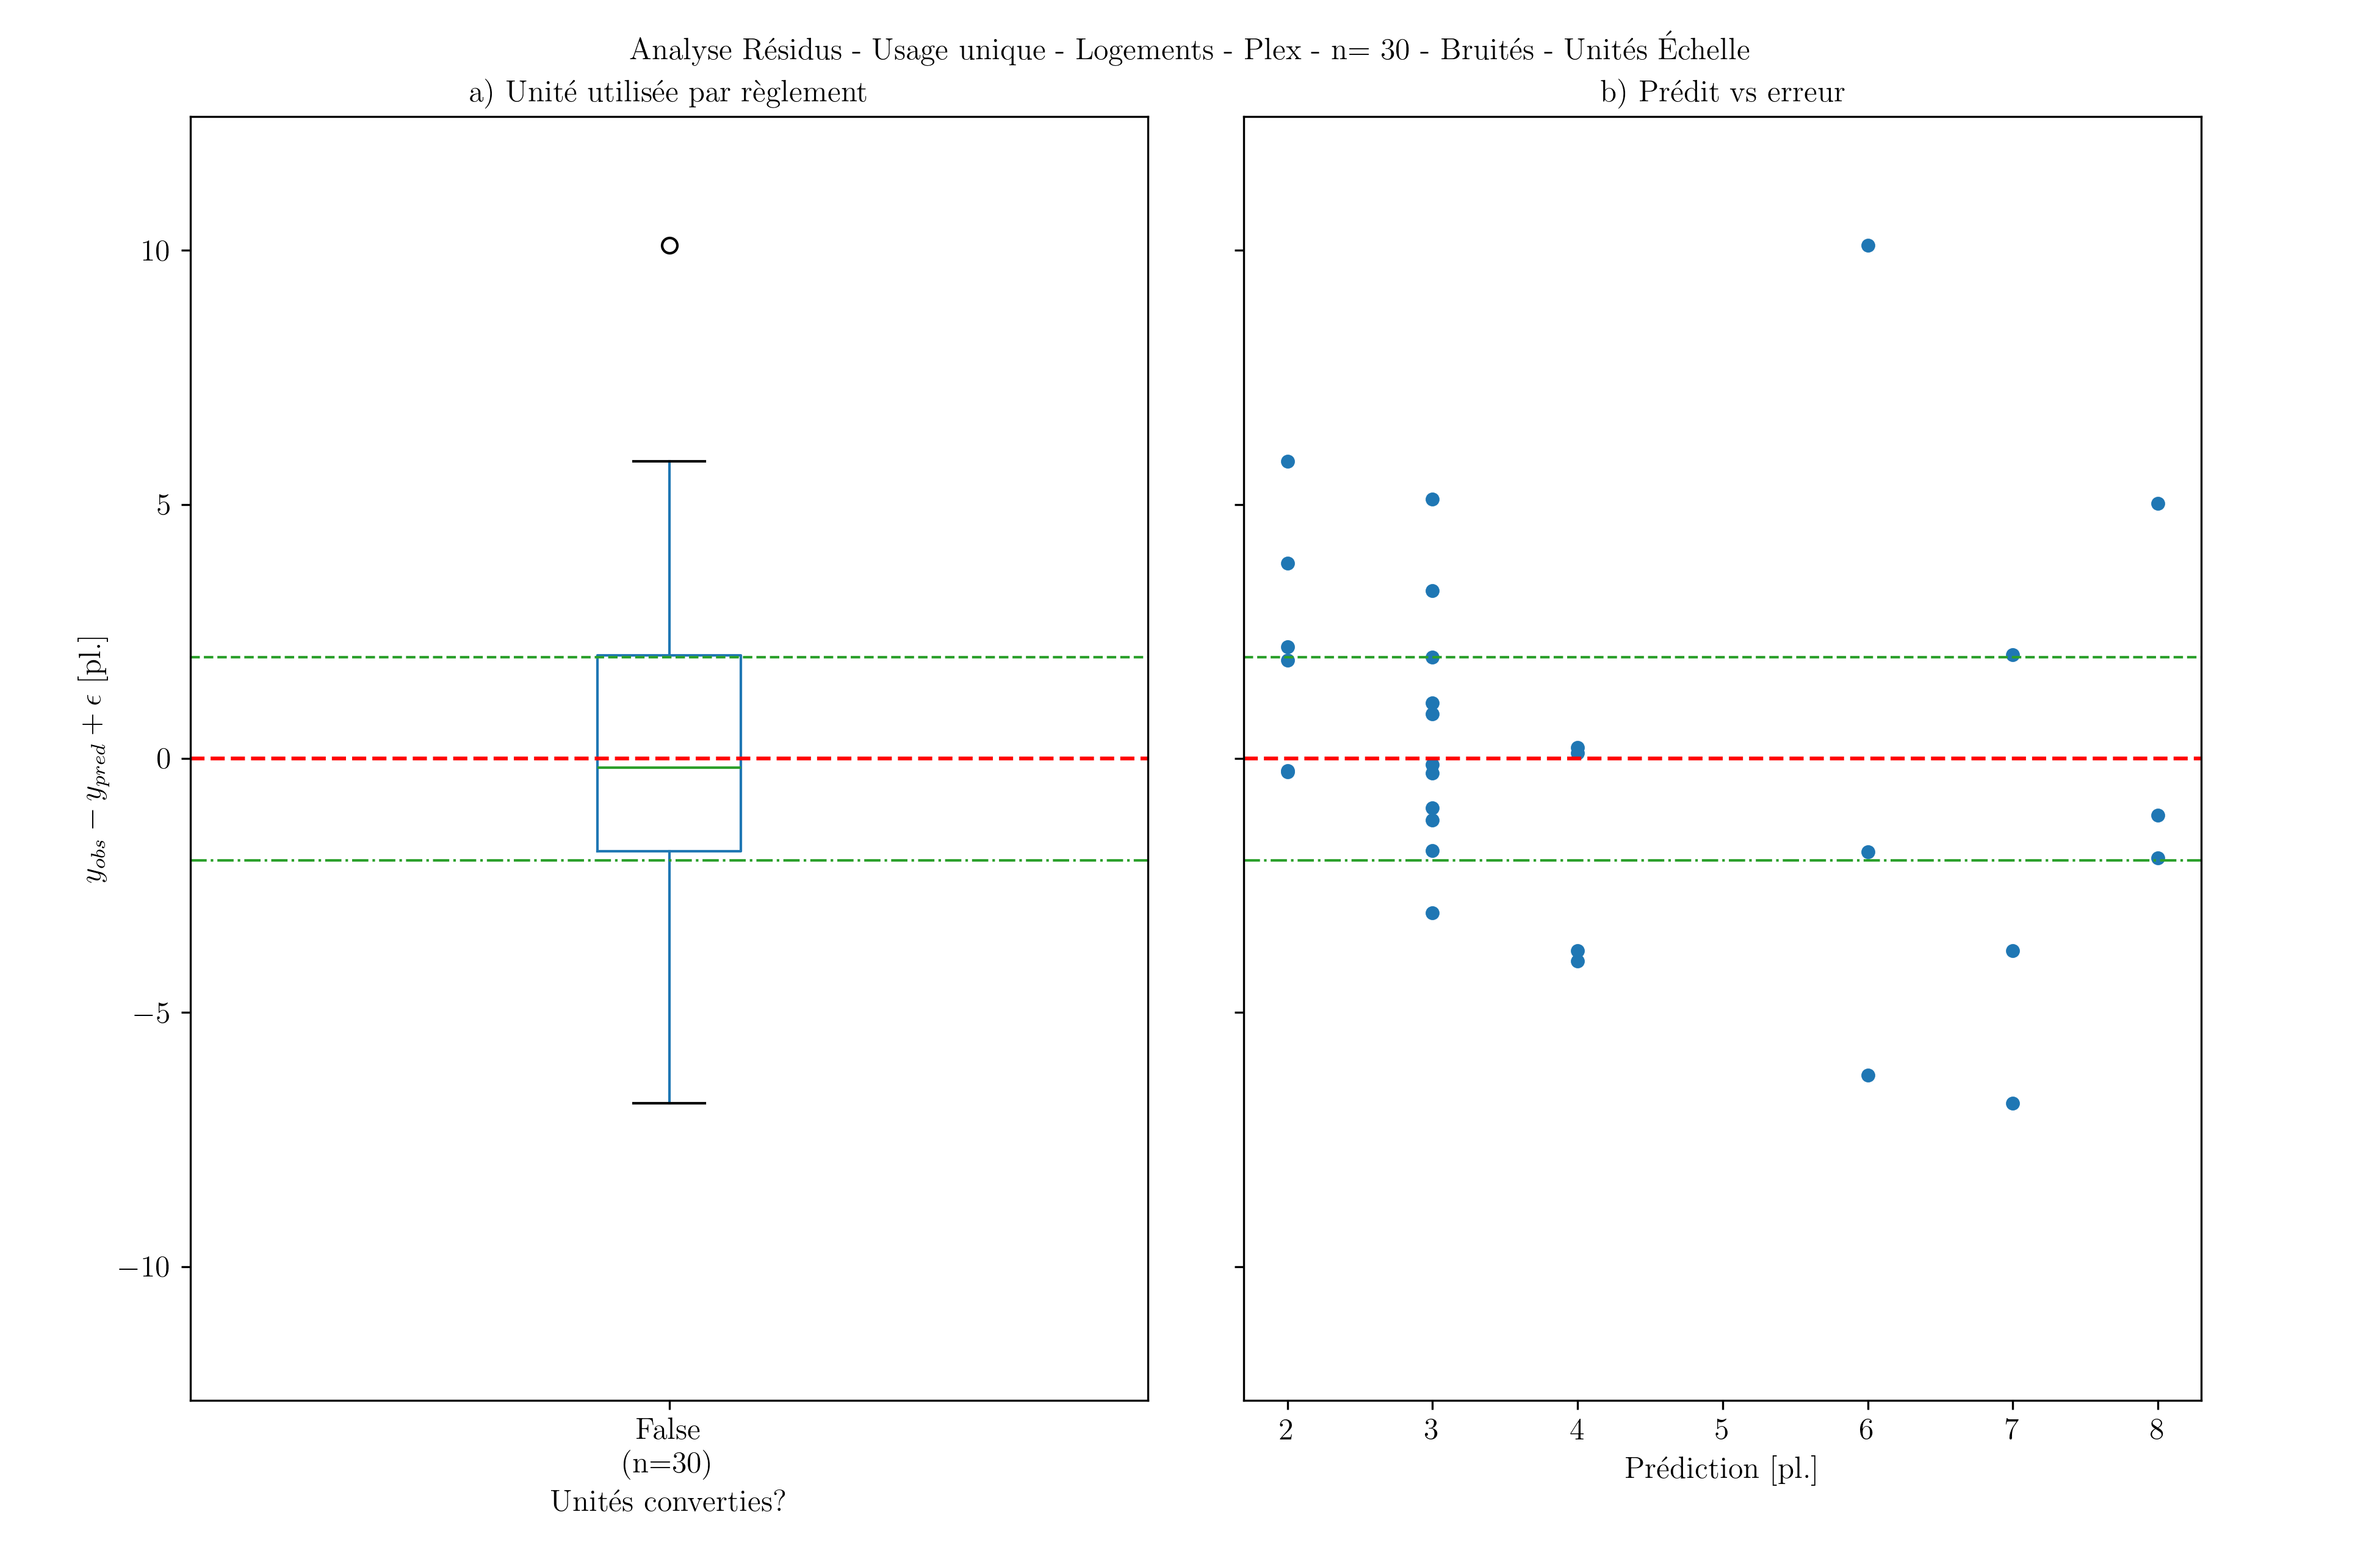
\includegraphics[width=1\linewidth]{images/ana_res_43_b_se_2_c.png}
        \caption{Analyse des résidus en fonction de la prédiction et des unités de formulation pour les lots avec 2 à 8 logements}
        \label{fig:ana-res-unit-pred-log-plex}
    \end{figure}
    \begin{figure}[H]
        \centering
        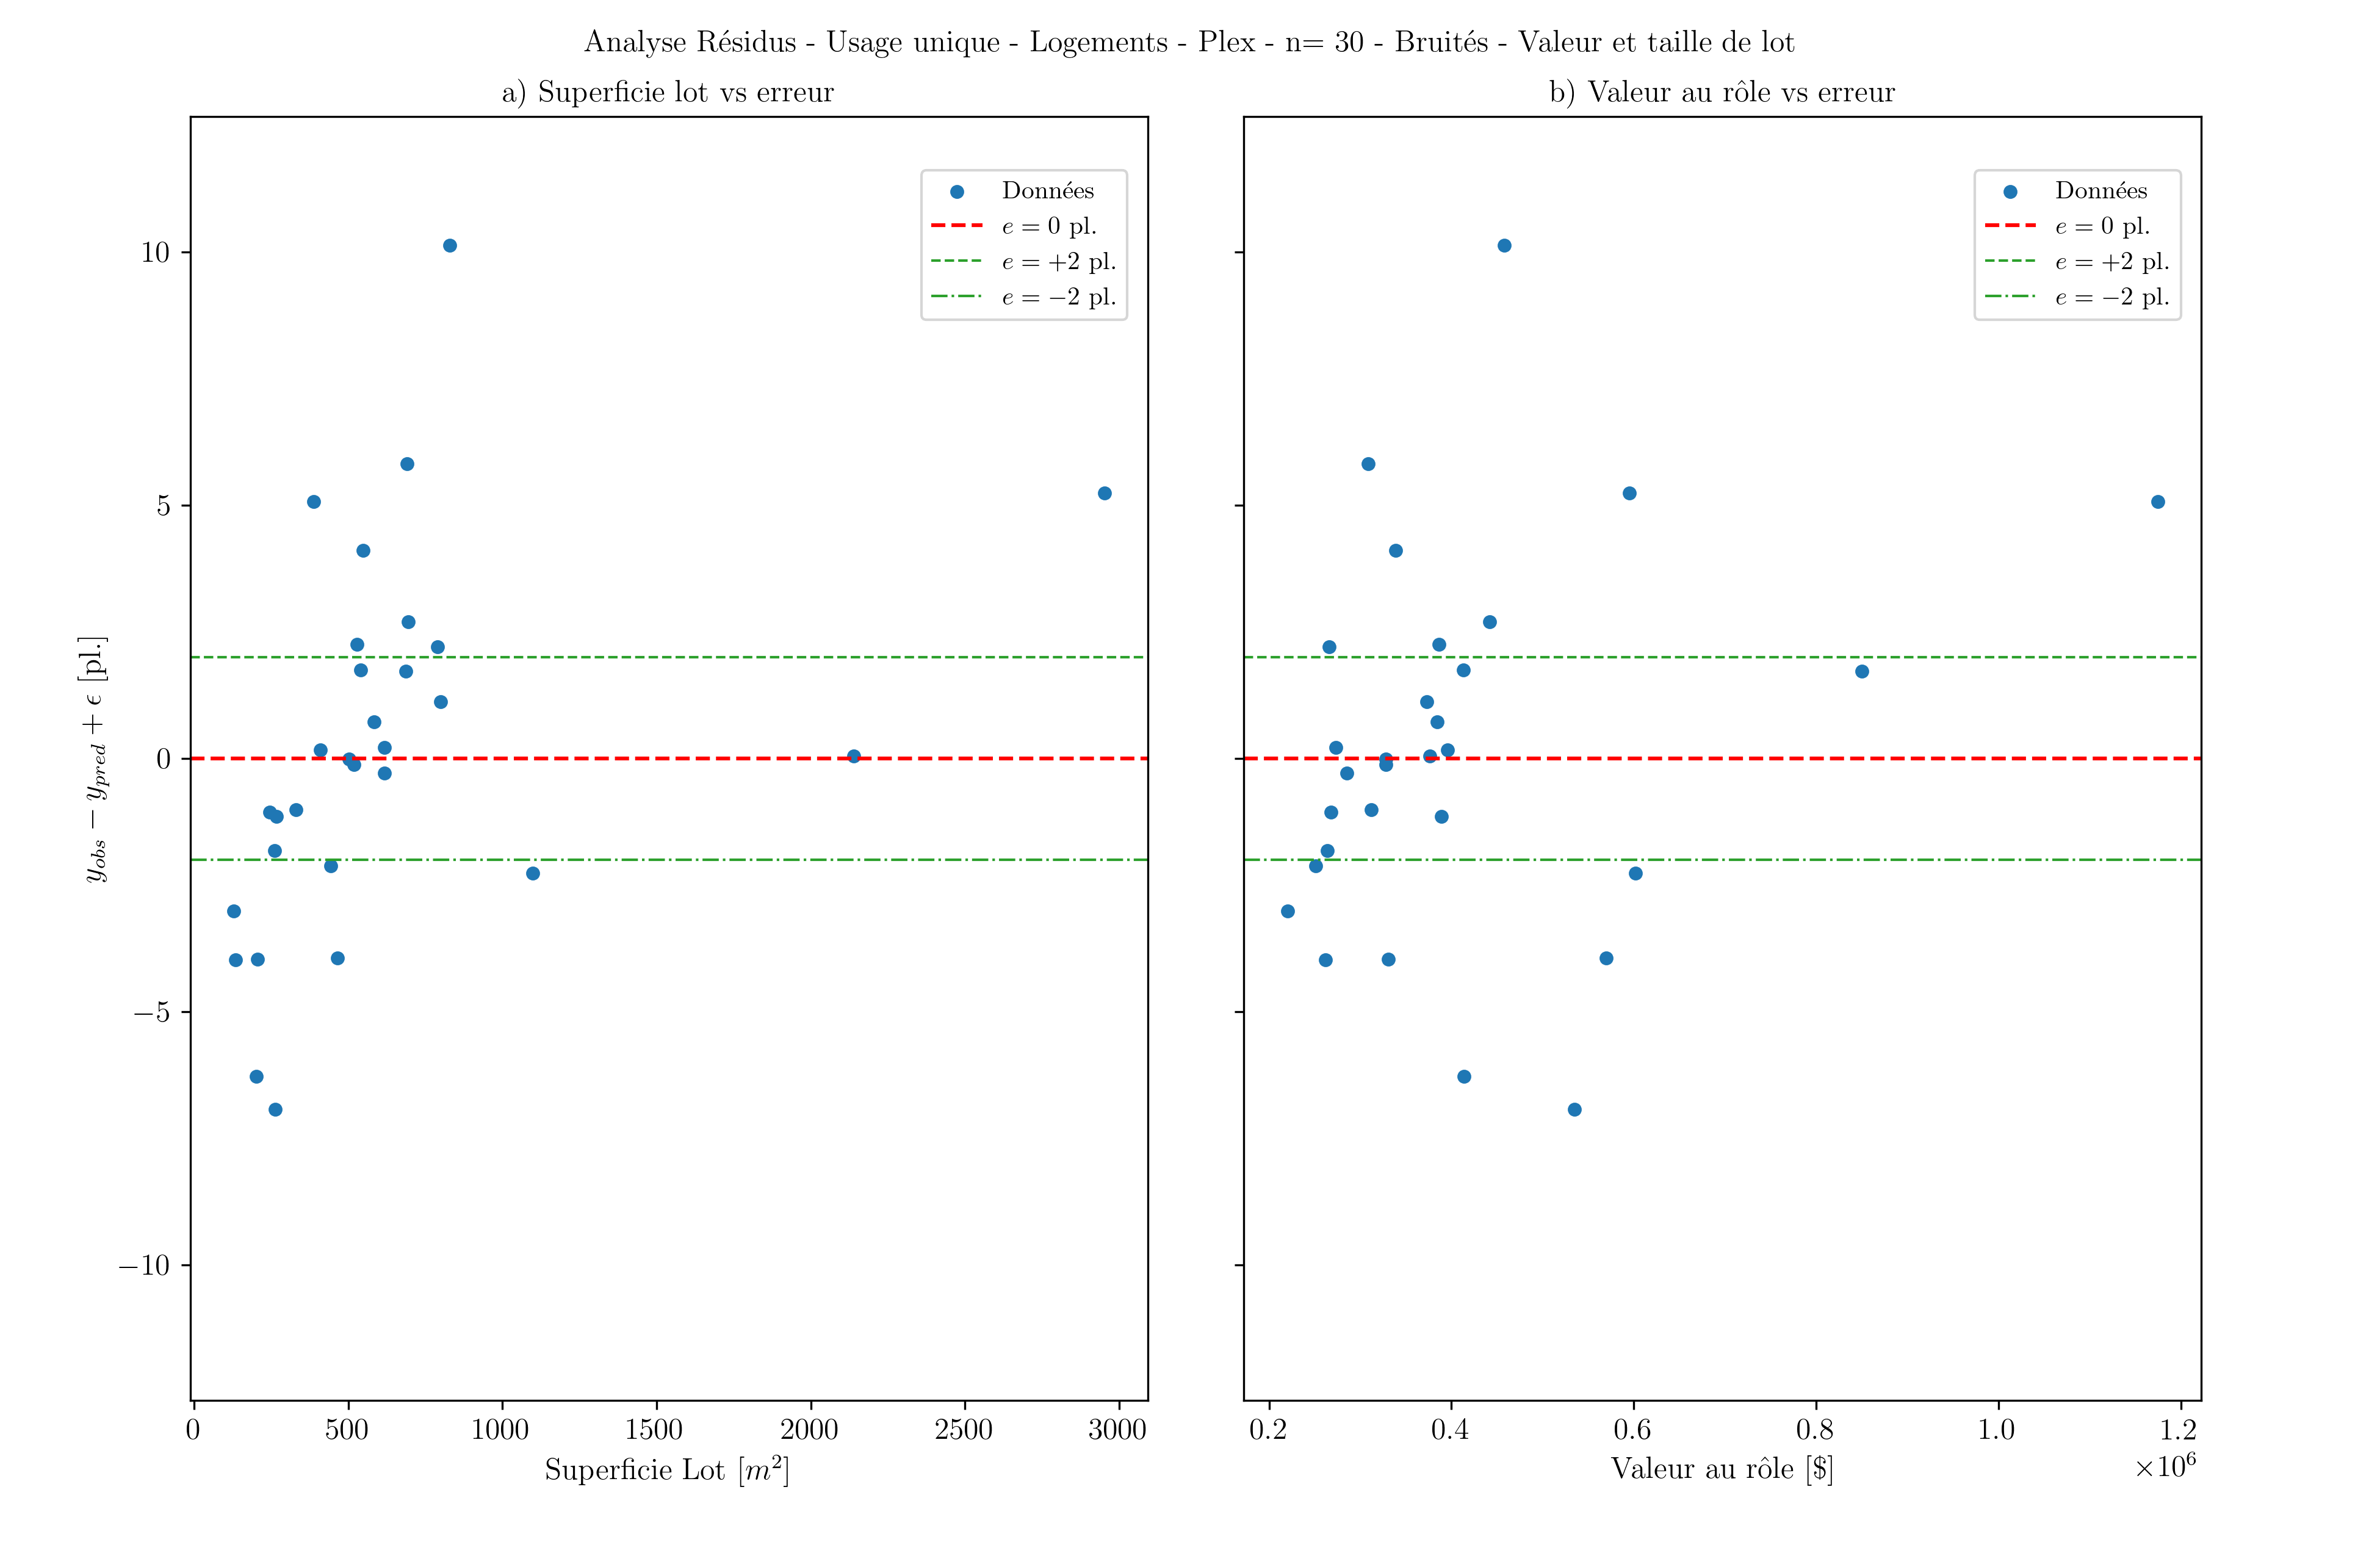
\includegraphics[width=1\linewidth]{images/ana_res_43_b_se_2_d.png}
        \caption{Analyse des résidus en fonction de la superficie du lot et de la valeur pour les lots avec 2 à 8 logements}
        \label{fig:ana-res-sup-val-log-plex}
    \end{figure}
    \begin{figure}[H]
        \centering
        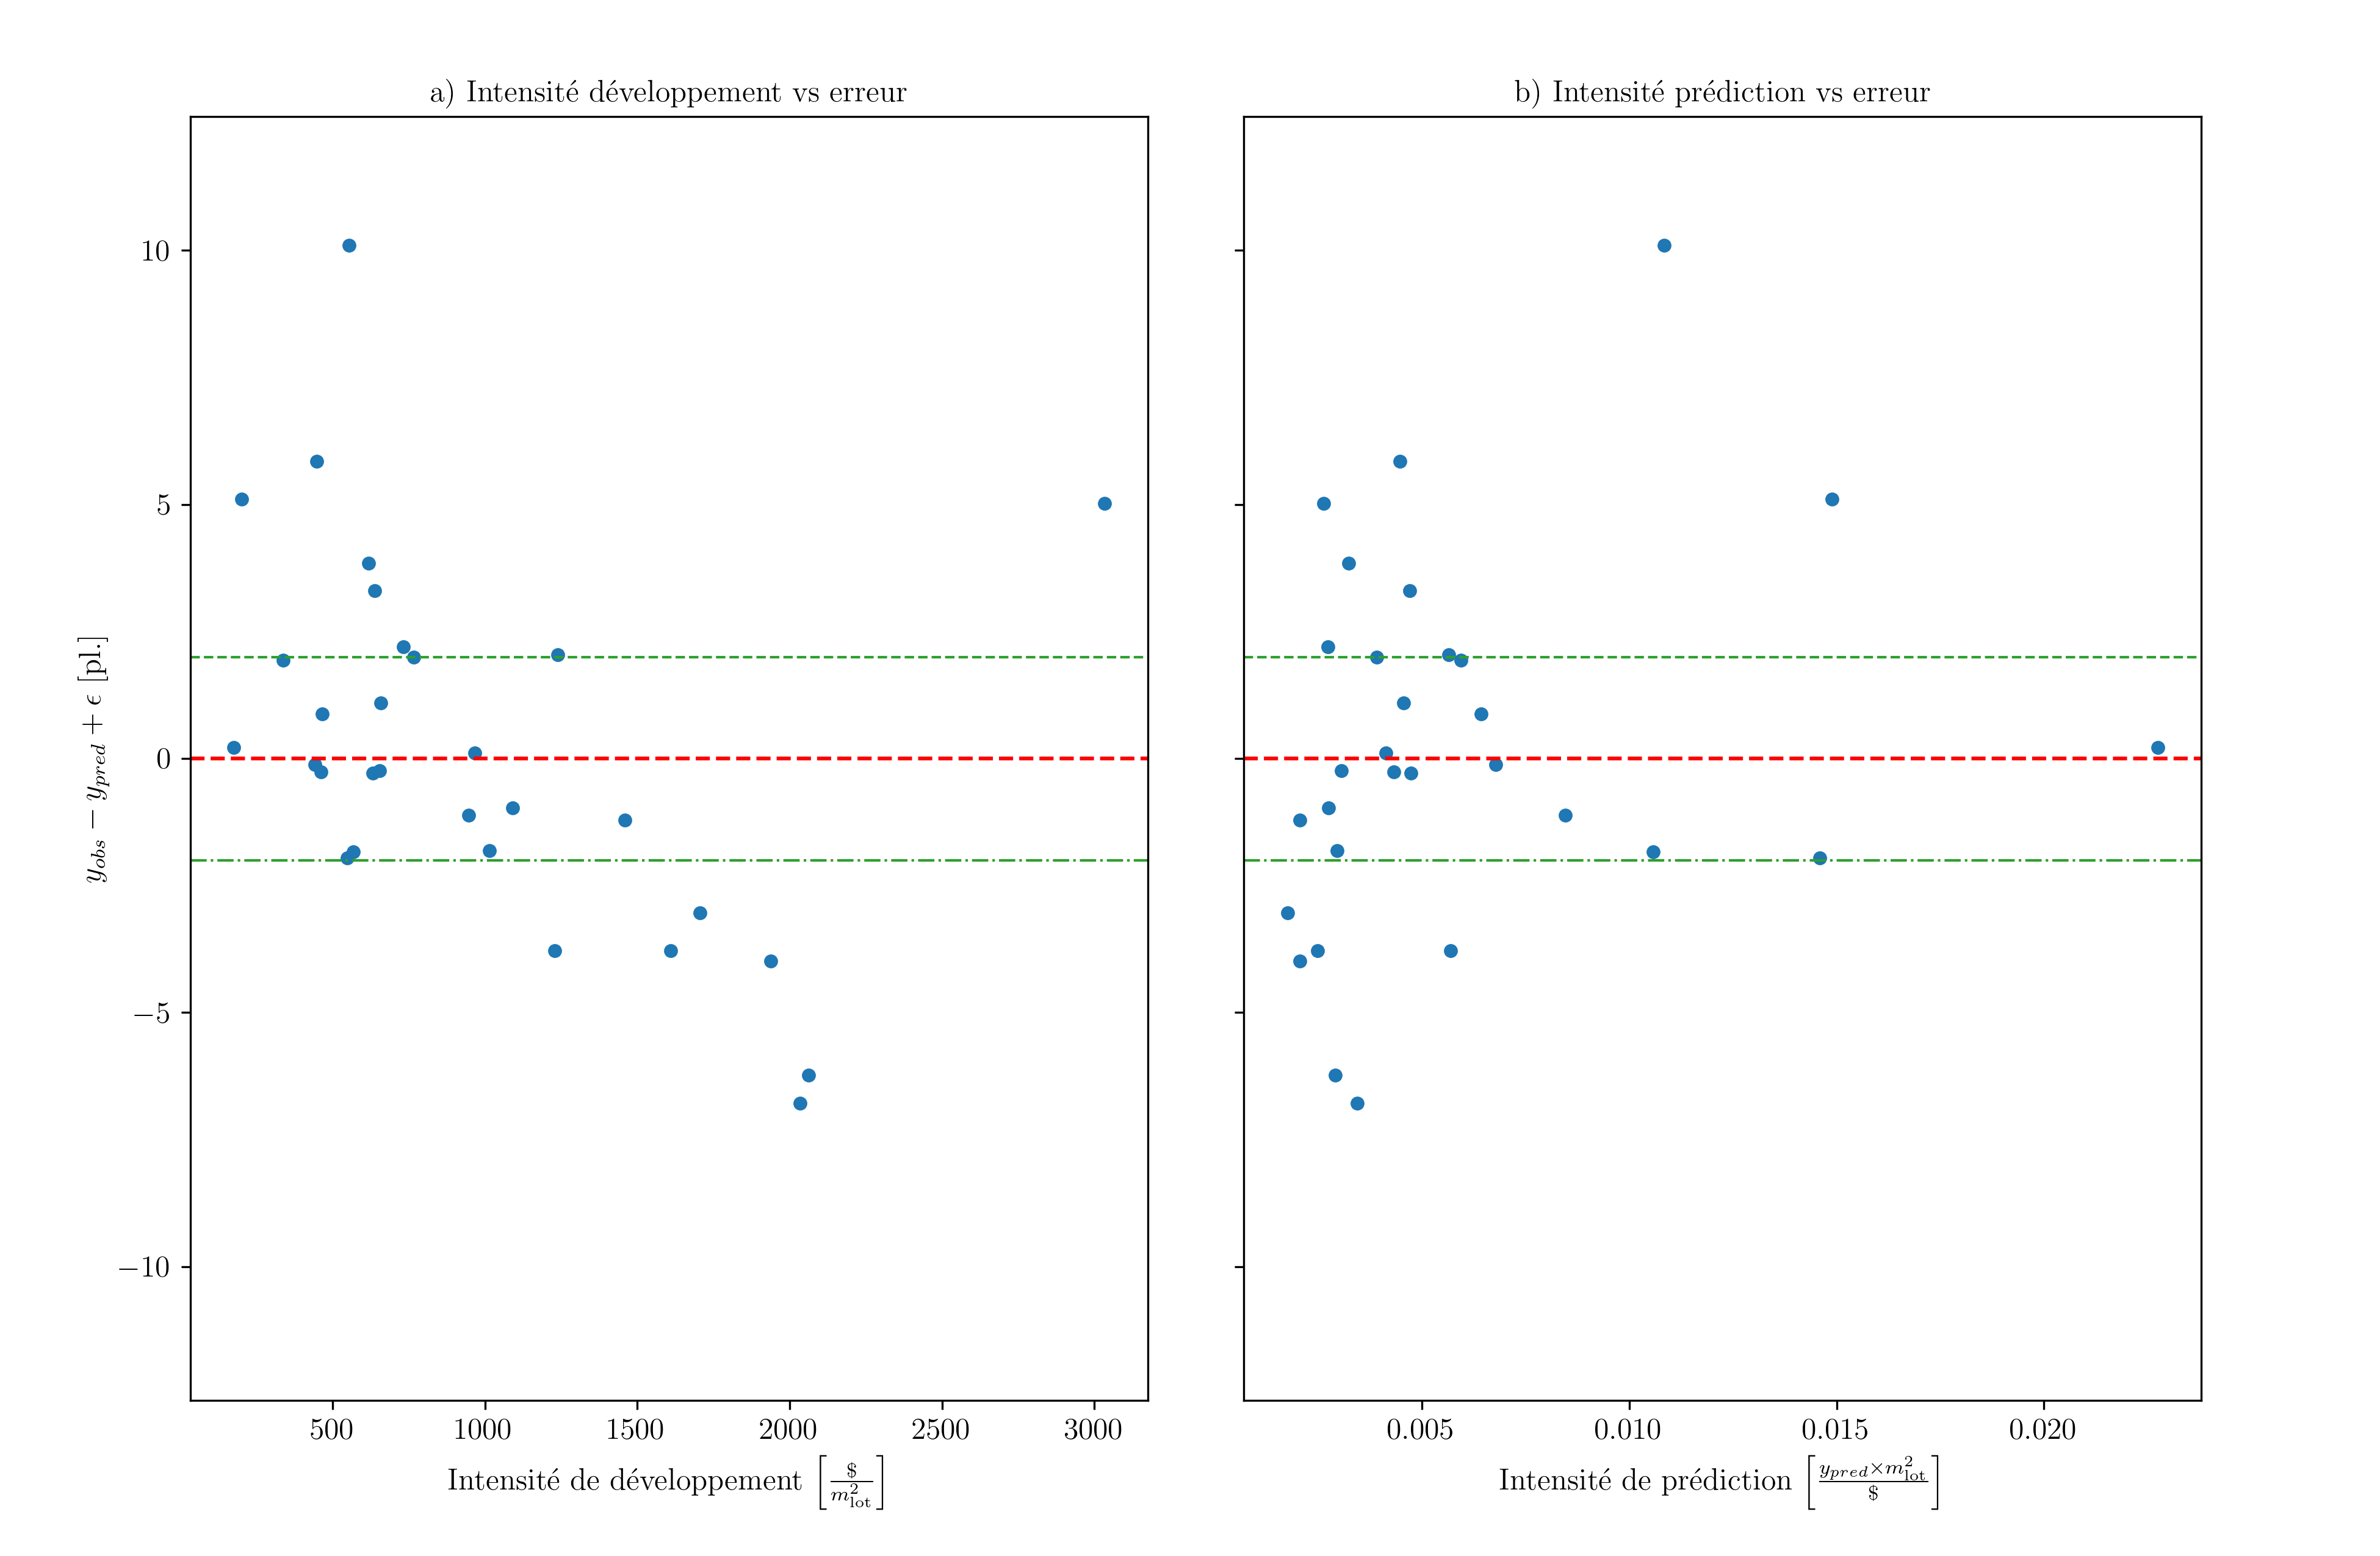
\includegraphics[width=1\linewidth]{images/ana_res_43_b_se_2_e.png}
        \caption{Analyse des résidus en fonction de l'intensité de développement et l'intensité de prédiction pour les lots avec 2 à 8 logements}
        \label{fig:ana-res-intens-log-plex}
    \end{figure}
\end{landscape}
\subsection{Résidentiel - Grands immeubles résidentiels}
Vingt-quatre immeubles résidentiels de plus de 8 logements ont été échantillonnés pour comparer la valeur observée à la valeur prédite. L'étendue des valeurs prédites est assez élevée que le bruit aléatoire n'est plus requis. Le modèle semble bien représenter la tendance centrale, mais il existe encore une forte dispersion autour de cette dernière. Le nombre moyen de places prédites $\bar{y}_{pred}$  est de 21.0 contre 19.7 pour les places observées $\bar{y}_{obs}$ . 6 échantillons sélectionnés n'ont pas pu être observés du fait de la présence de stationnement souterrain. Aucune métrique ne permet de trouver les valeurs aberrantes. Aucune tendance claire n'émerge sur les mesures pouvant corriger l'erreur. 

\begin{landscape}
    %\begin{figure}
    %    \centering
    %    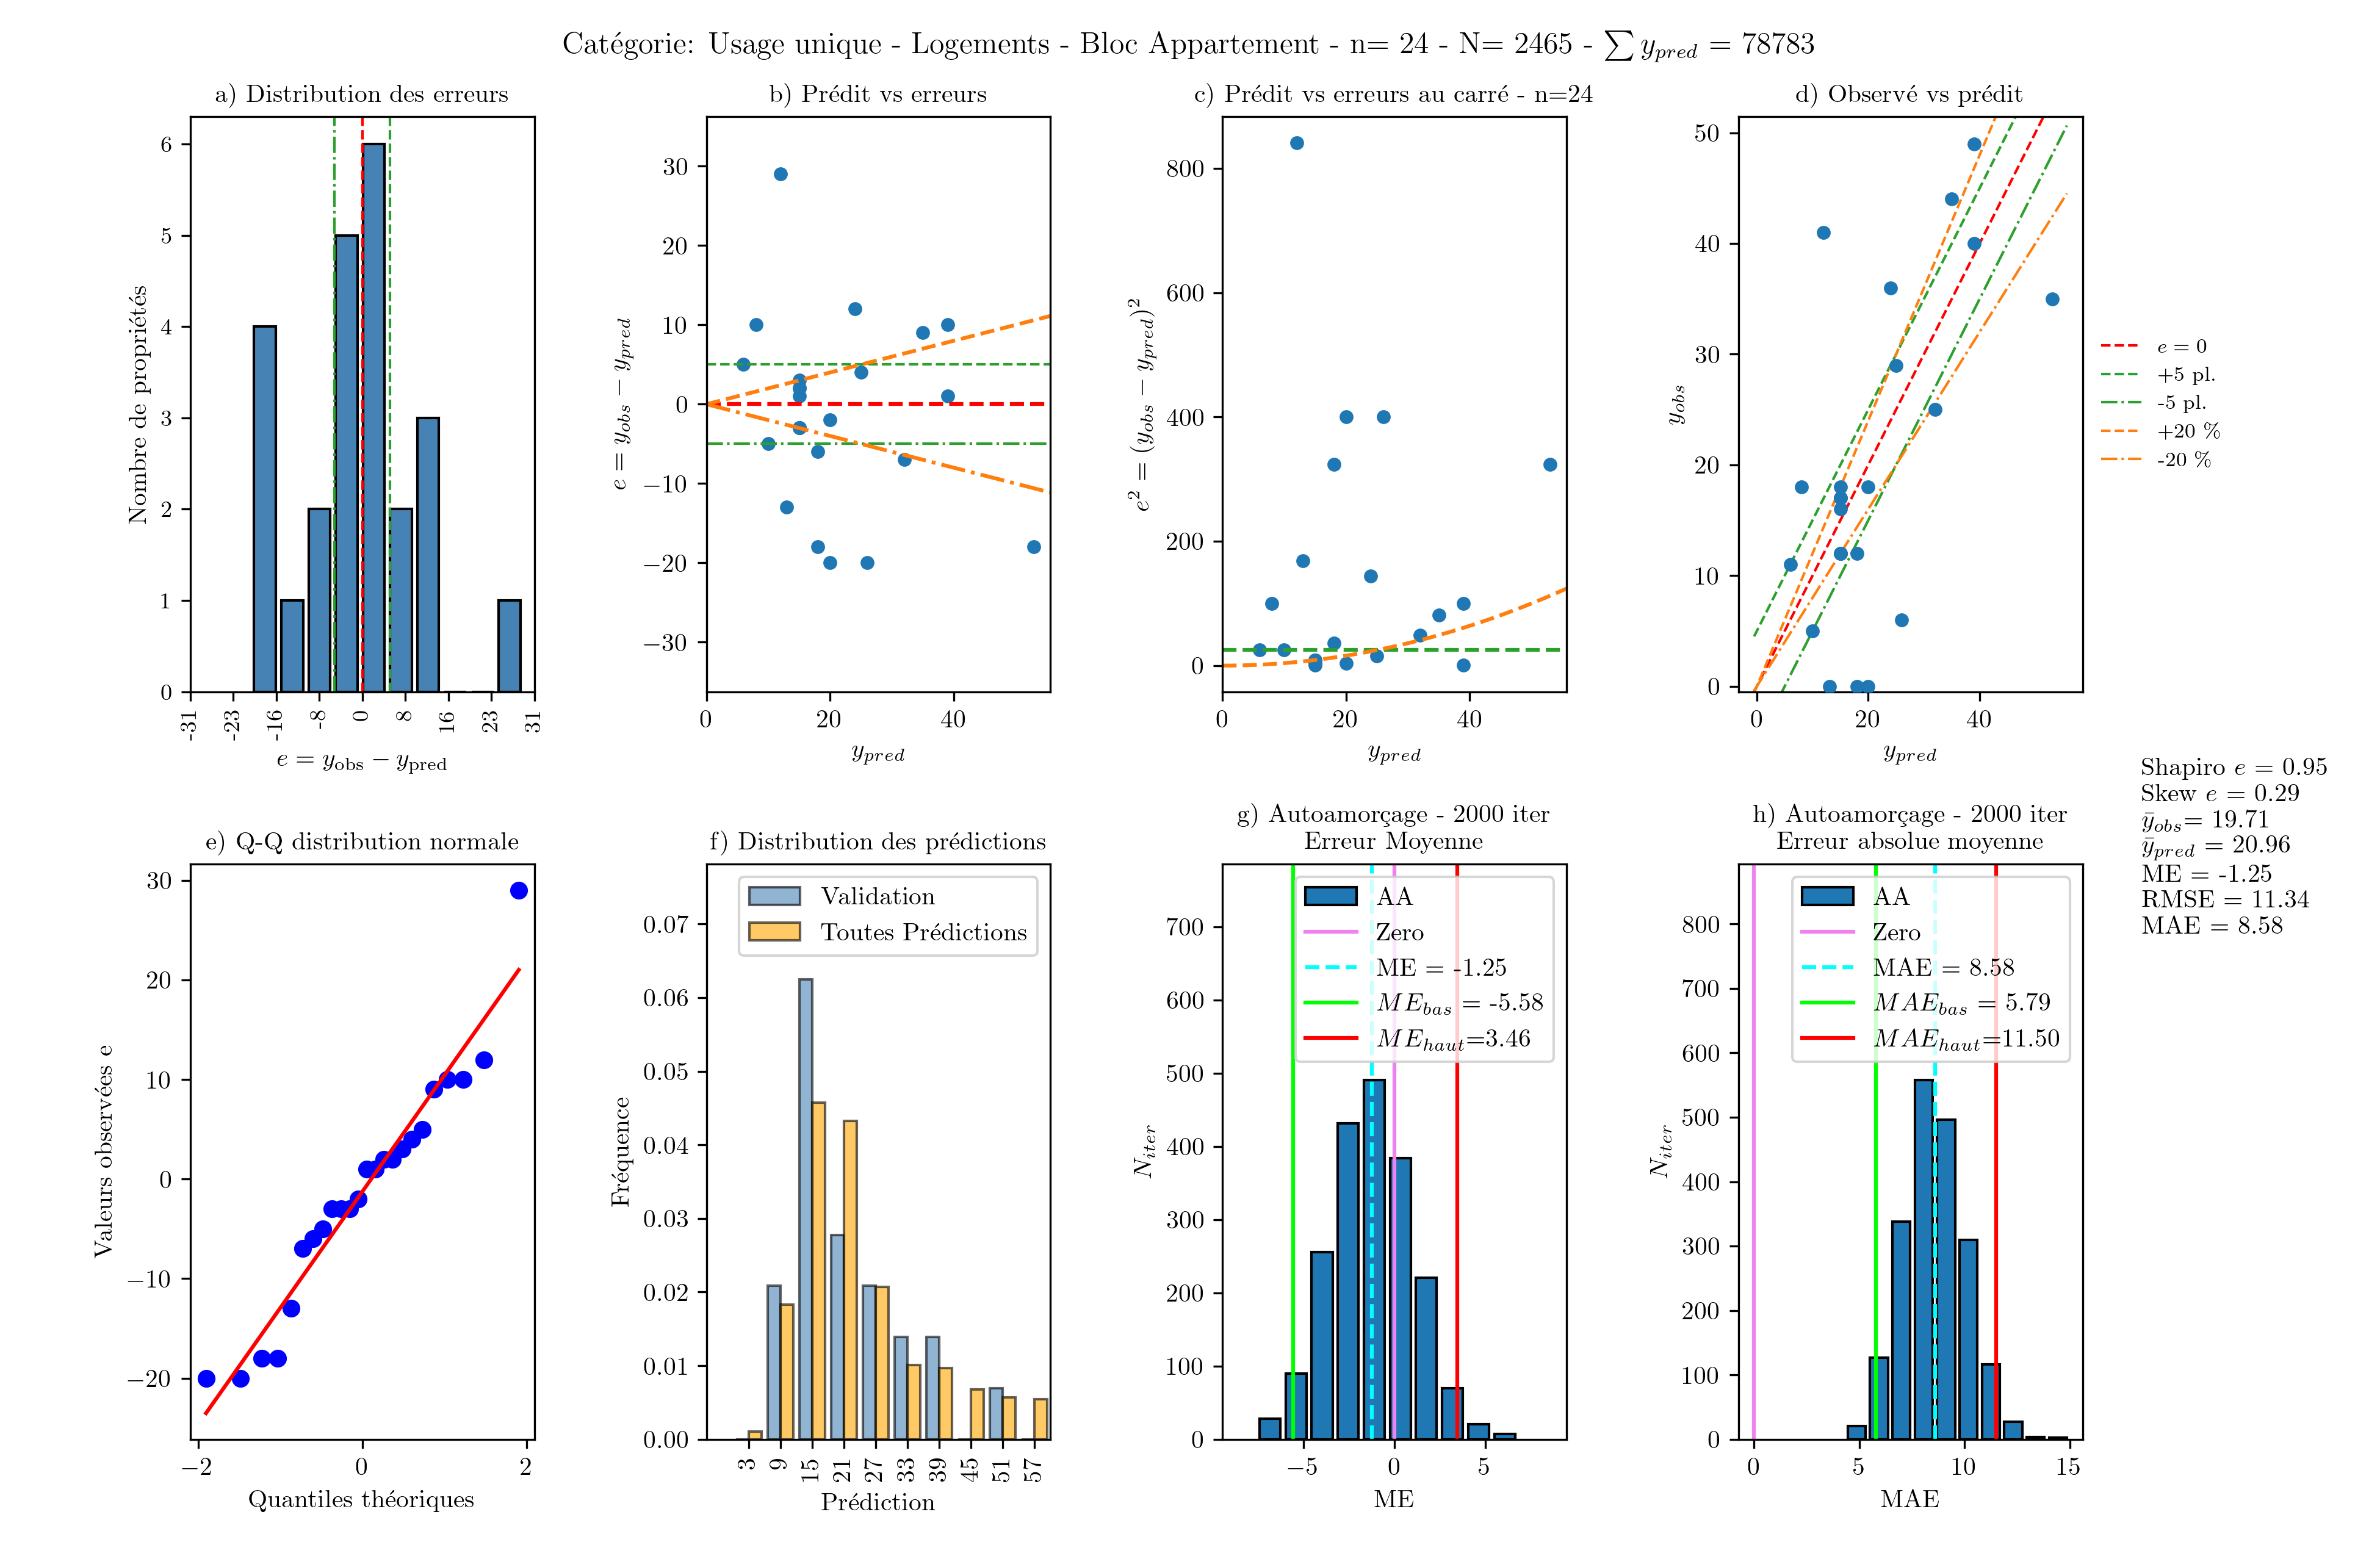
\includegraphics[scale=0.7]{images/int_erreur_44_se_5_pe_20.png}
    %    \caption{Distribution et intervalles d'erreurs pour les grands immeubles résidentiels}
    %    \label{fig:intervals-dist-val-log-bloc}
    %\end{figure}
    \begin{figure}[H]
        \centering
        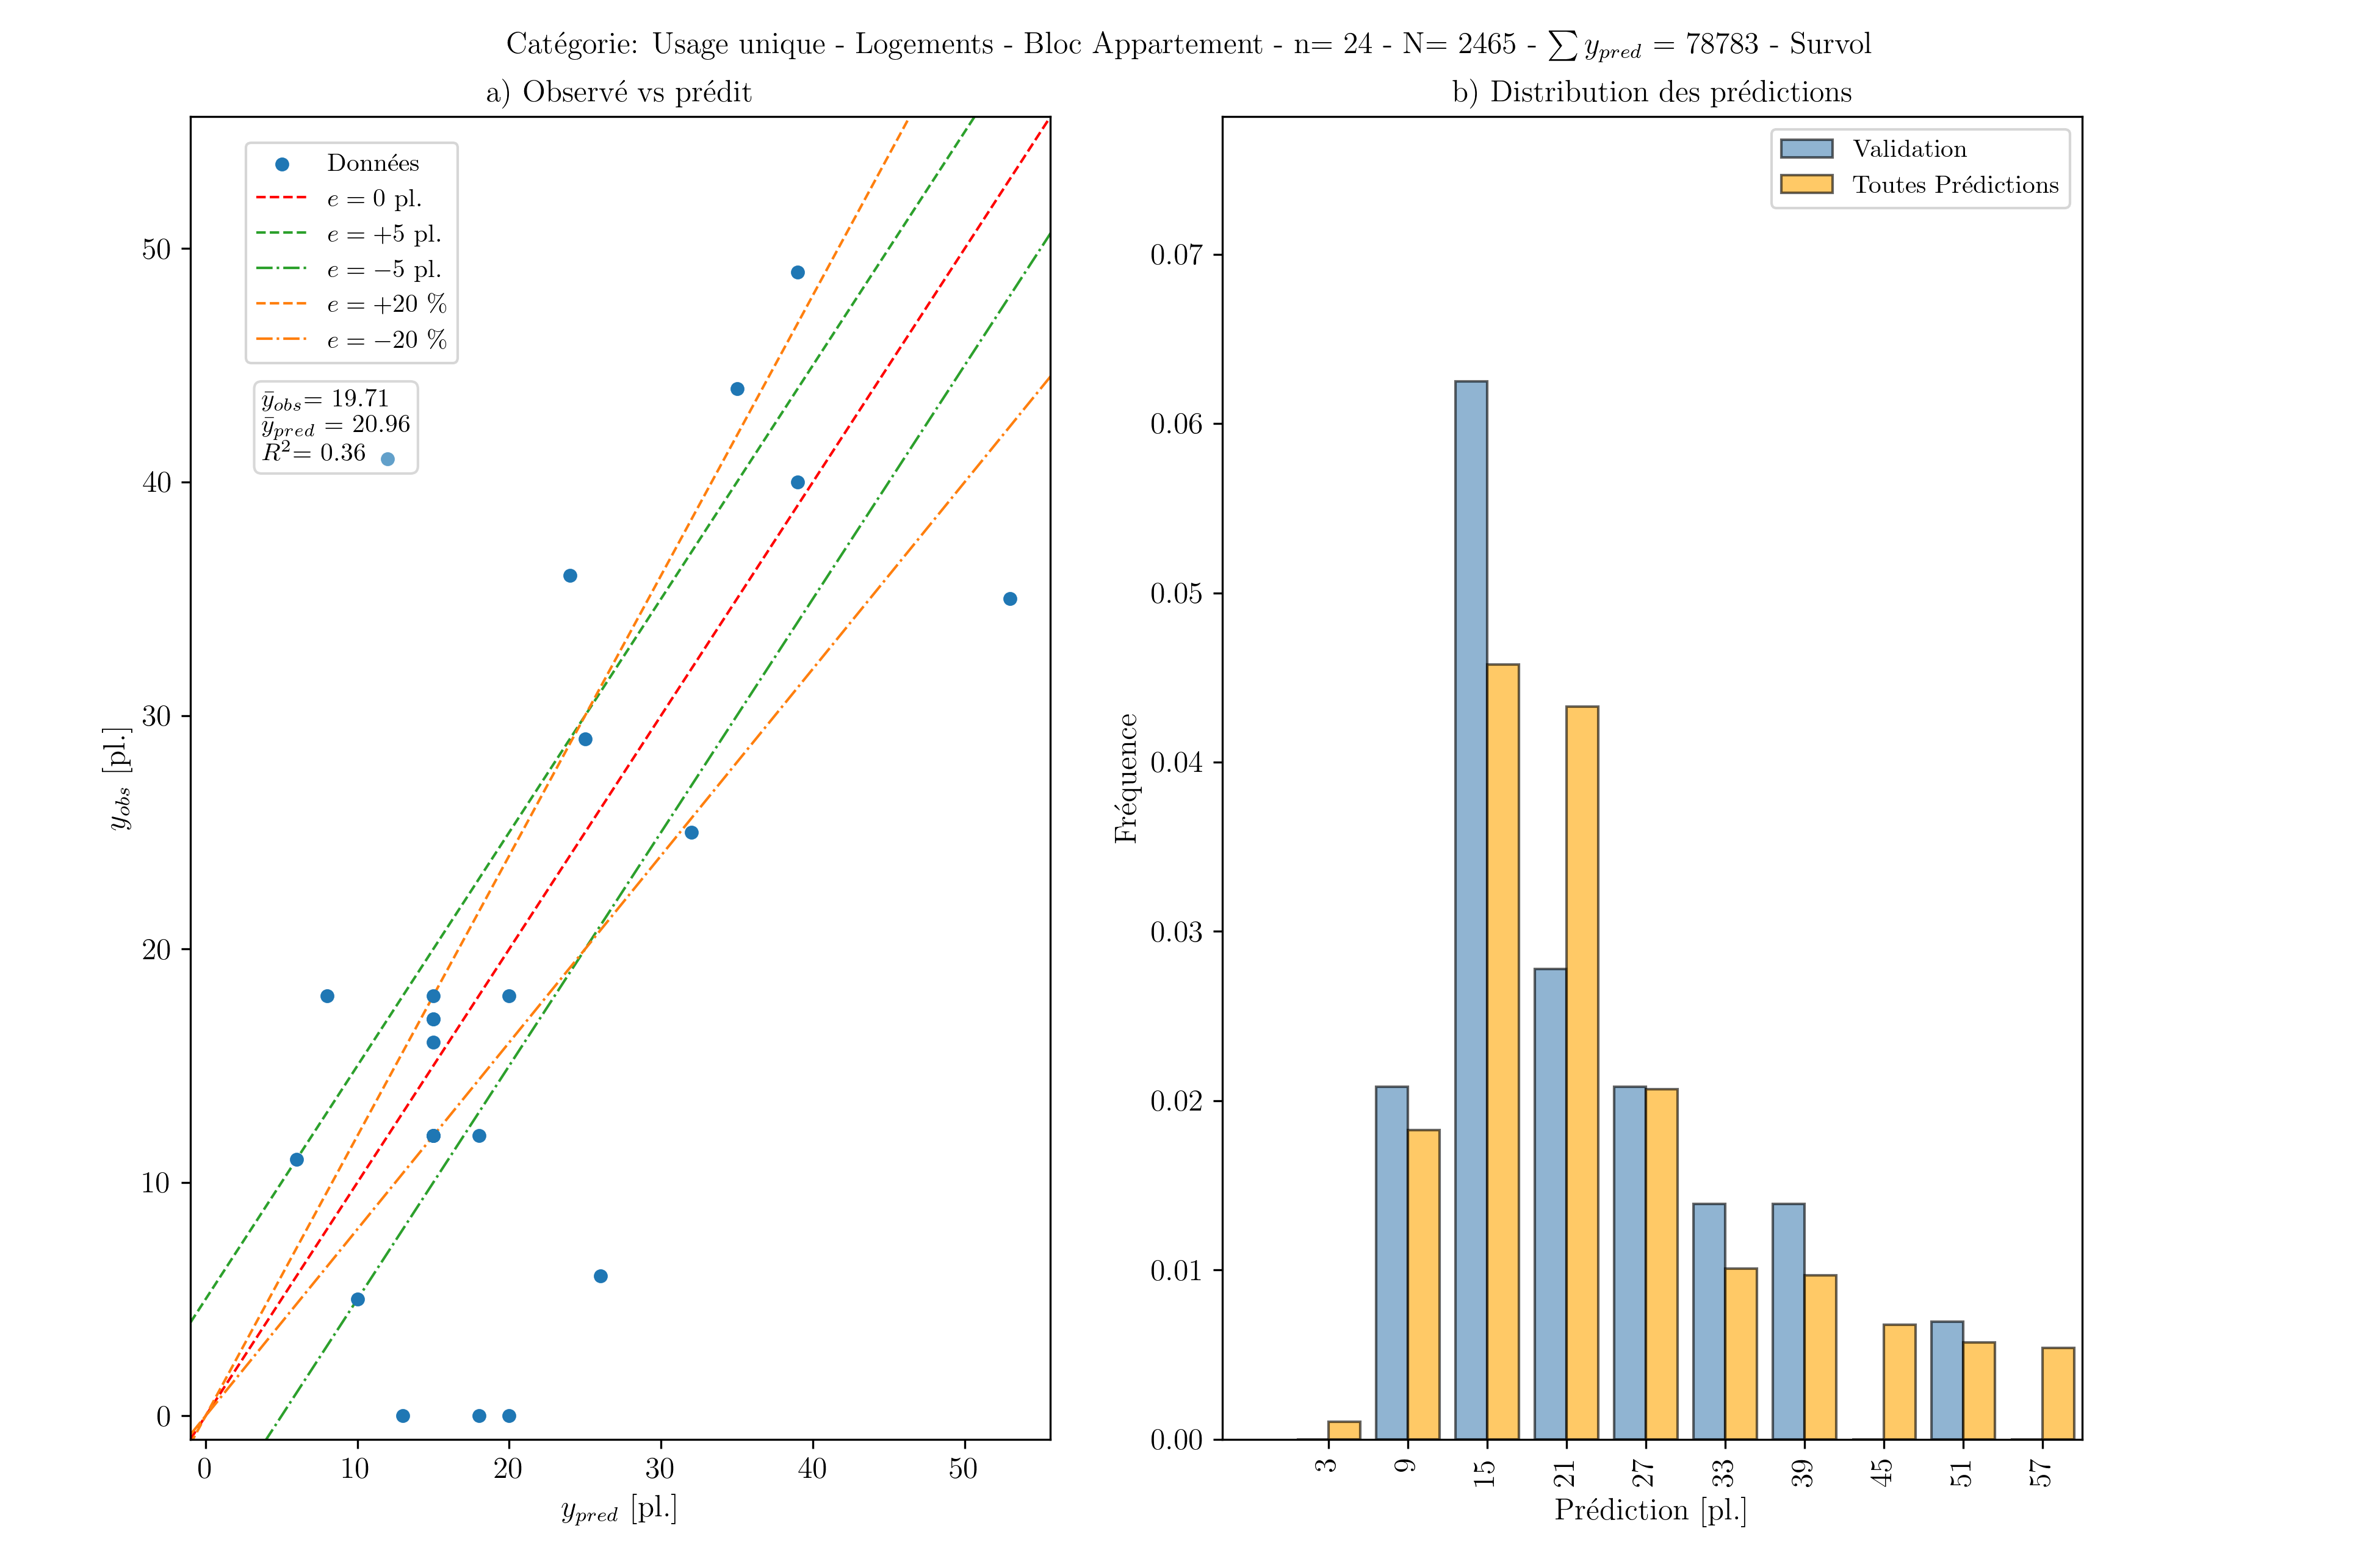
\includegraphics[width=1\linewidth]{images/int_erreur_44_se_5_pe_20_a.png}
        \caption{Distribution des prédictions pour les grands immeubles résidentiels}
        \label{fig:int-dist-pred-log-bloc}
    \end{figure}
    \begin{figure}[H]
        \centering
        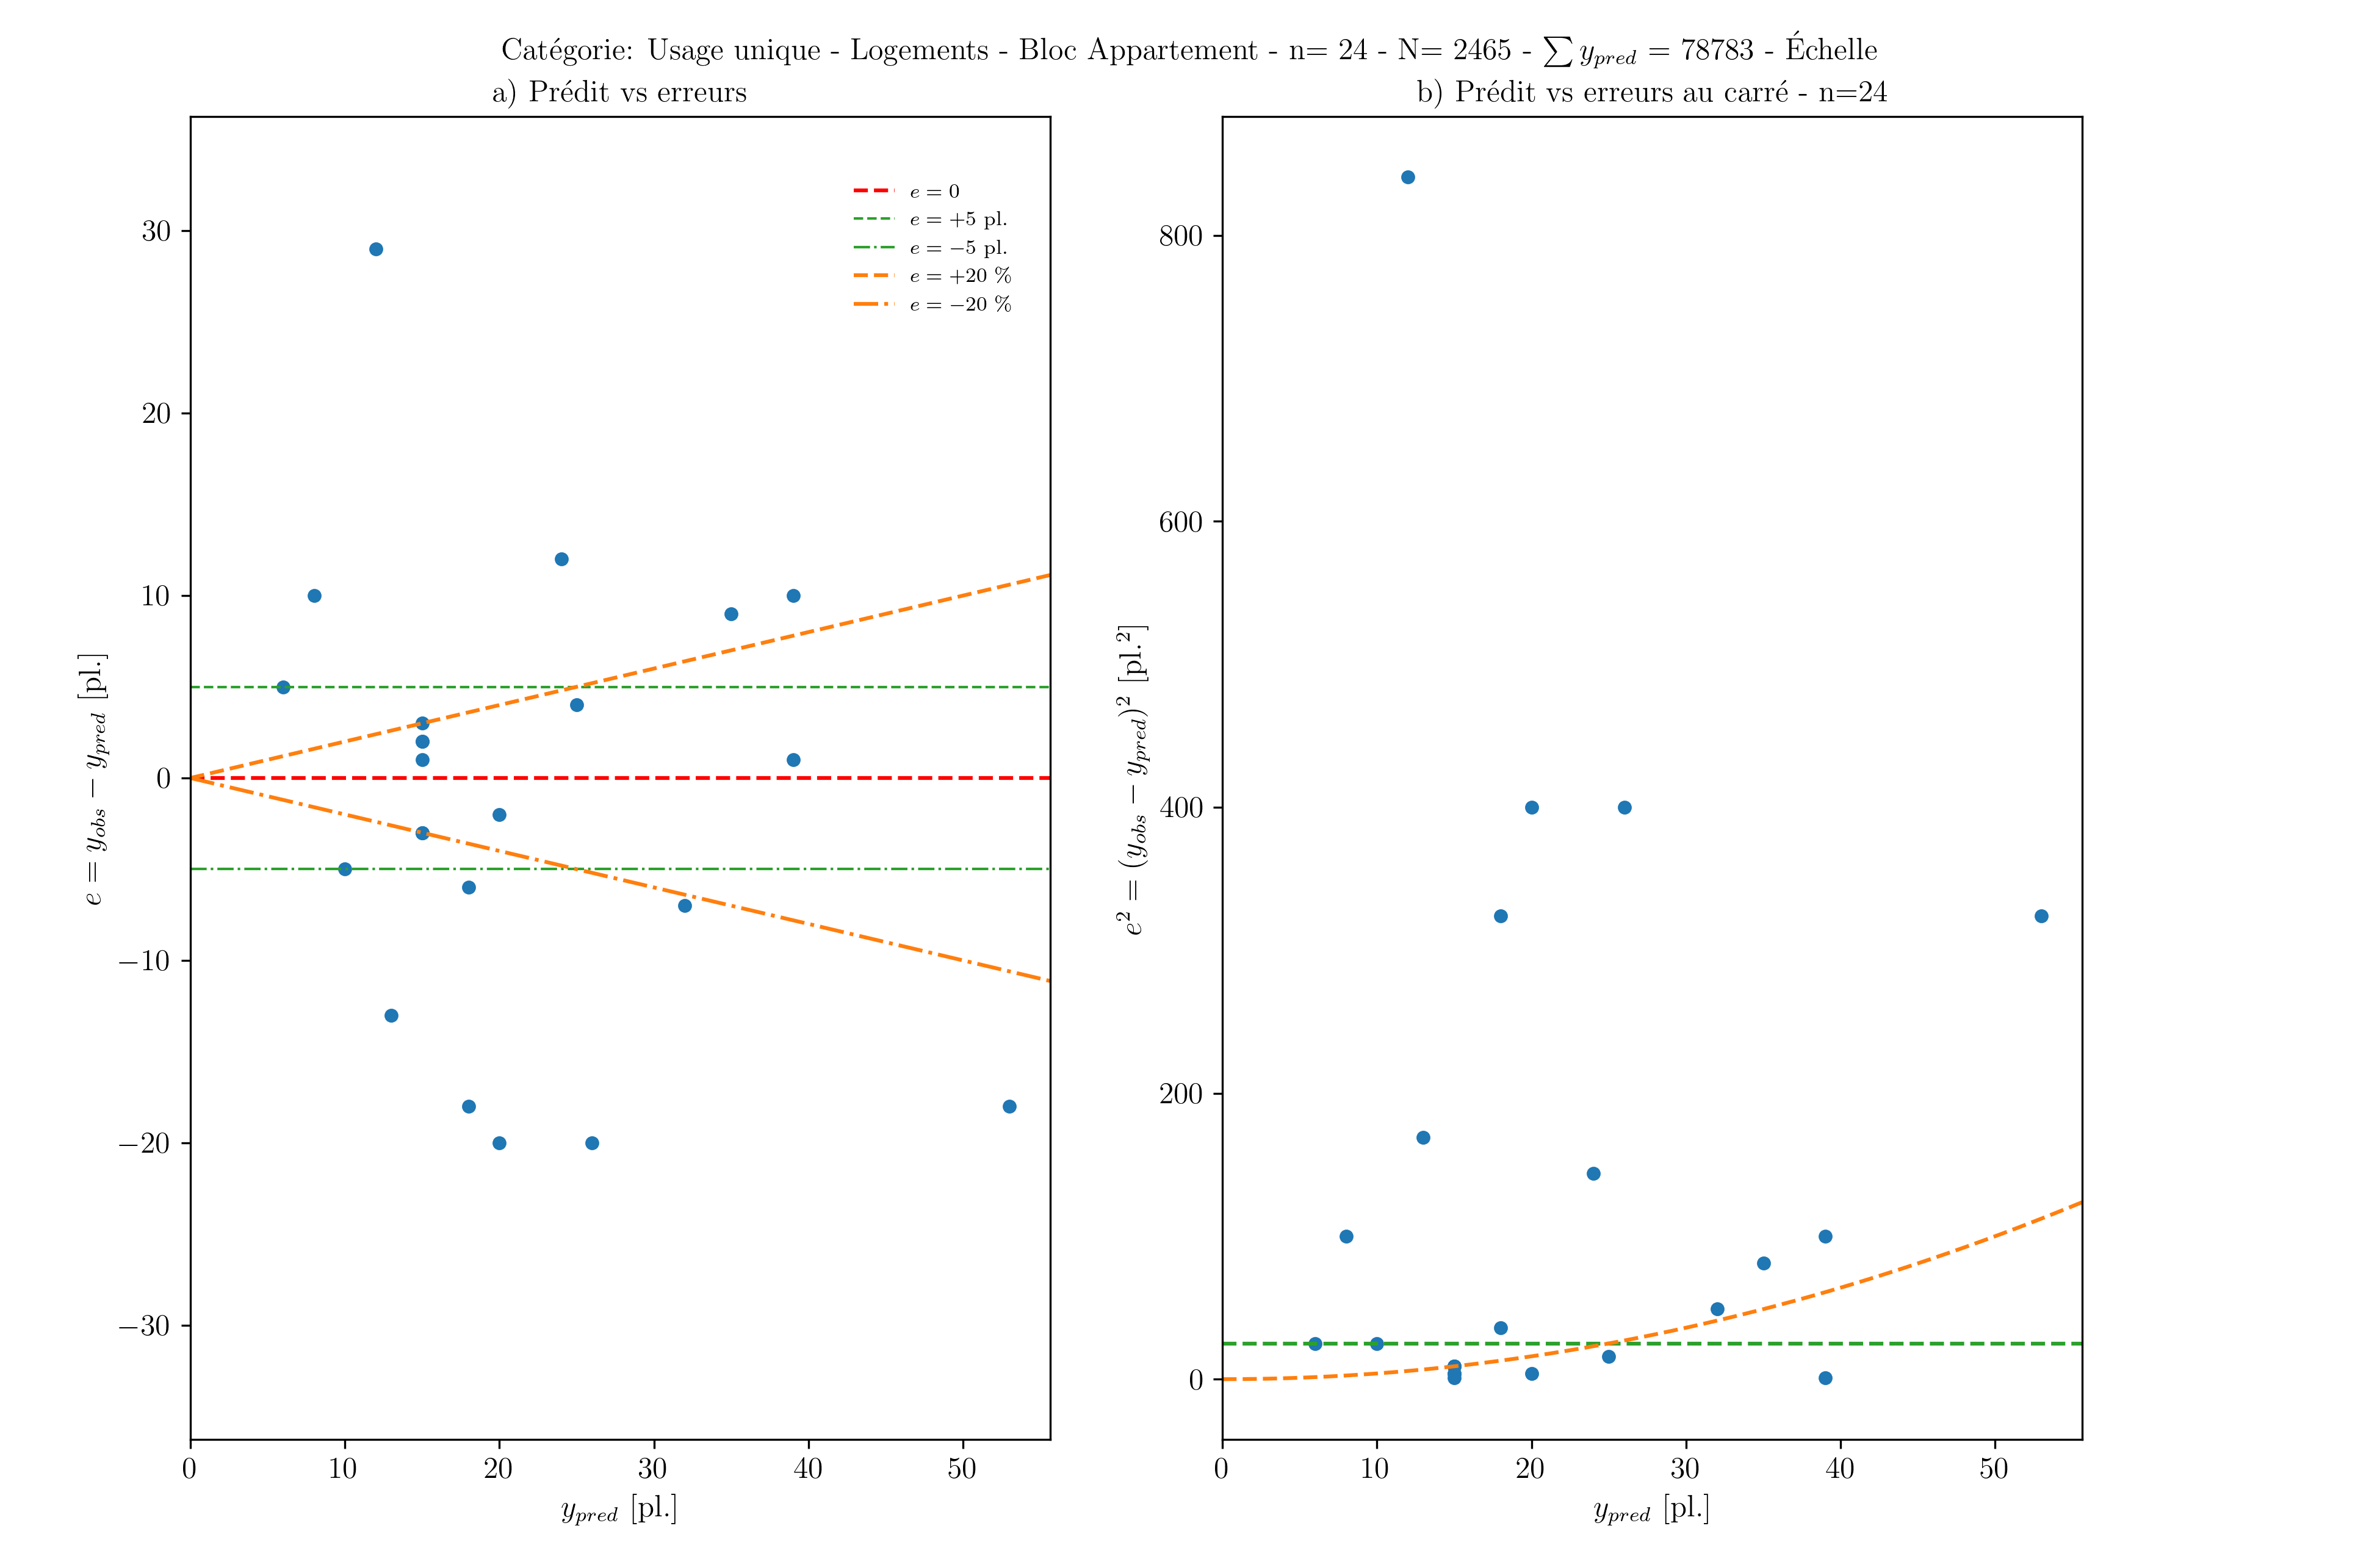
\includegraphics[width=1\linewidth]{images/int_erreur_44_se_5_pe_20_b.png}
        \caption{Erreur en fonction des prédictions pour les grands immeubles résidentiels}
        \label{fig:err-err-quad-pred-log-bloc}
    \end{figure}
    \begin{figure}[H]
        \centering
        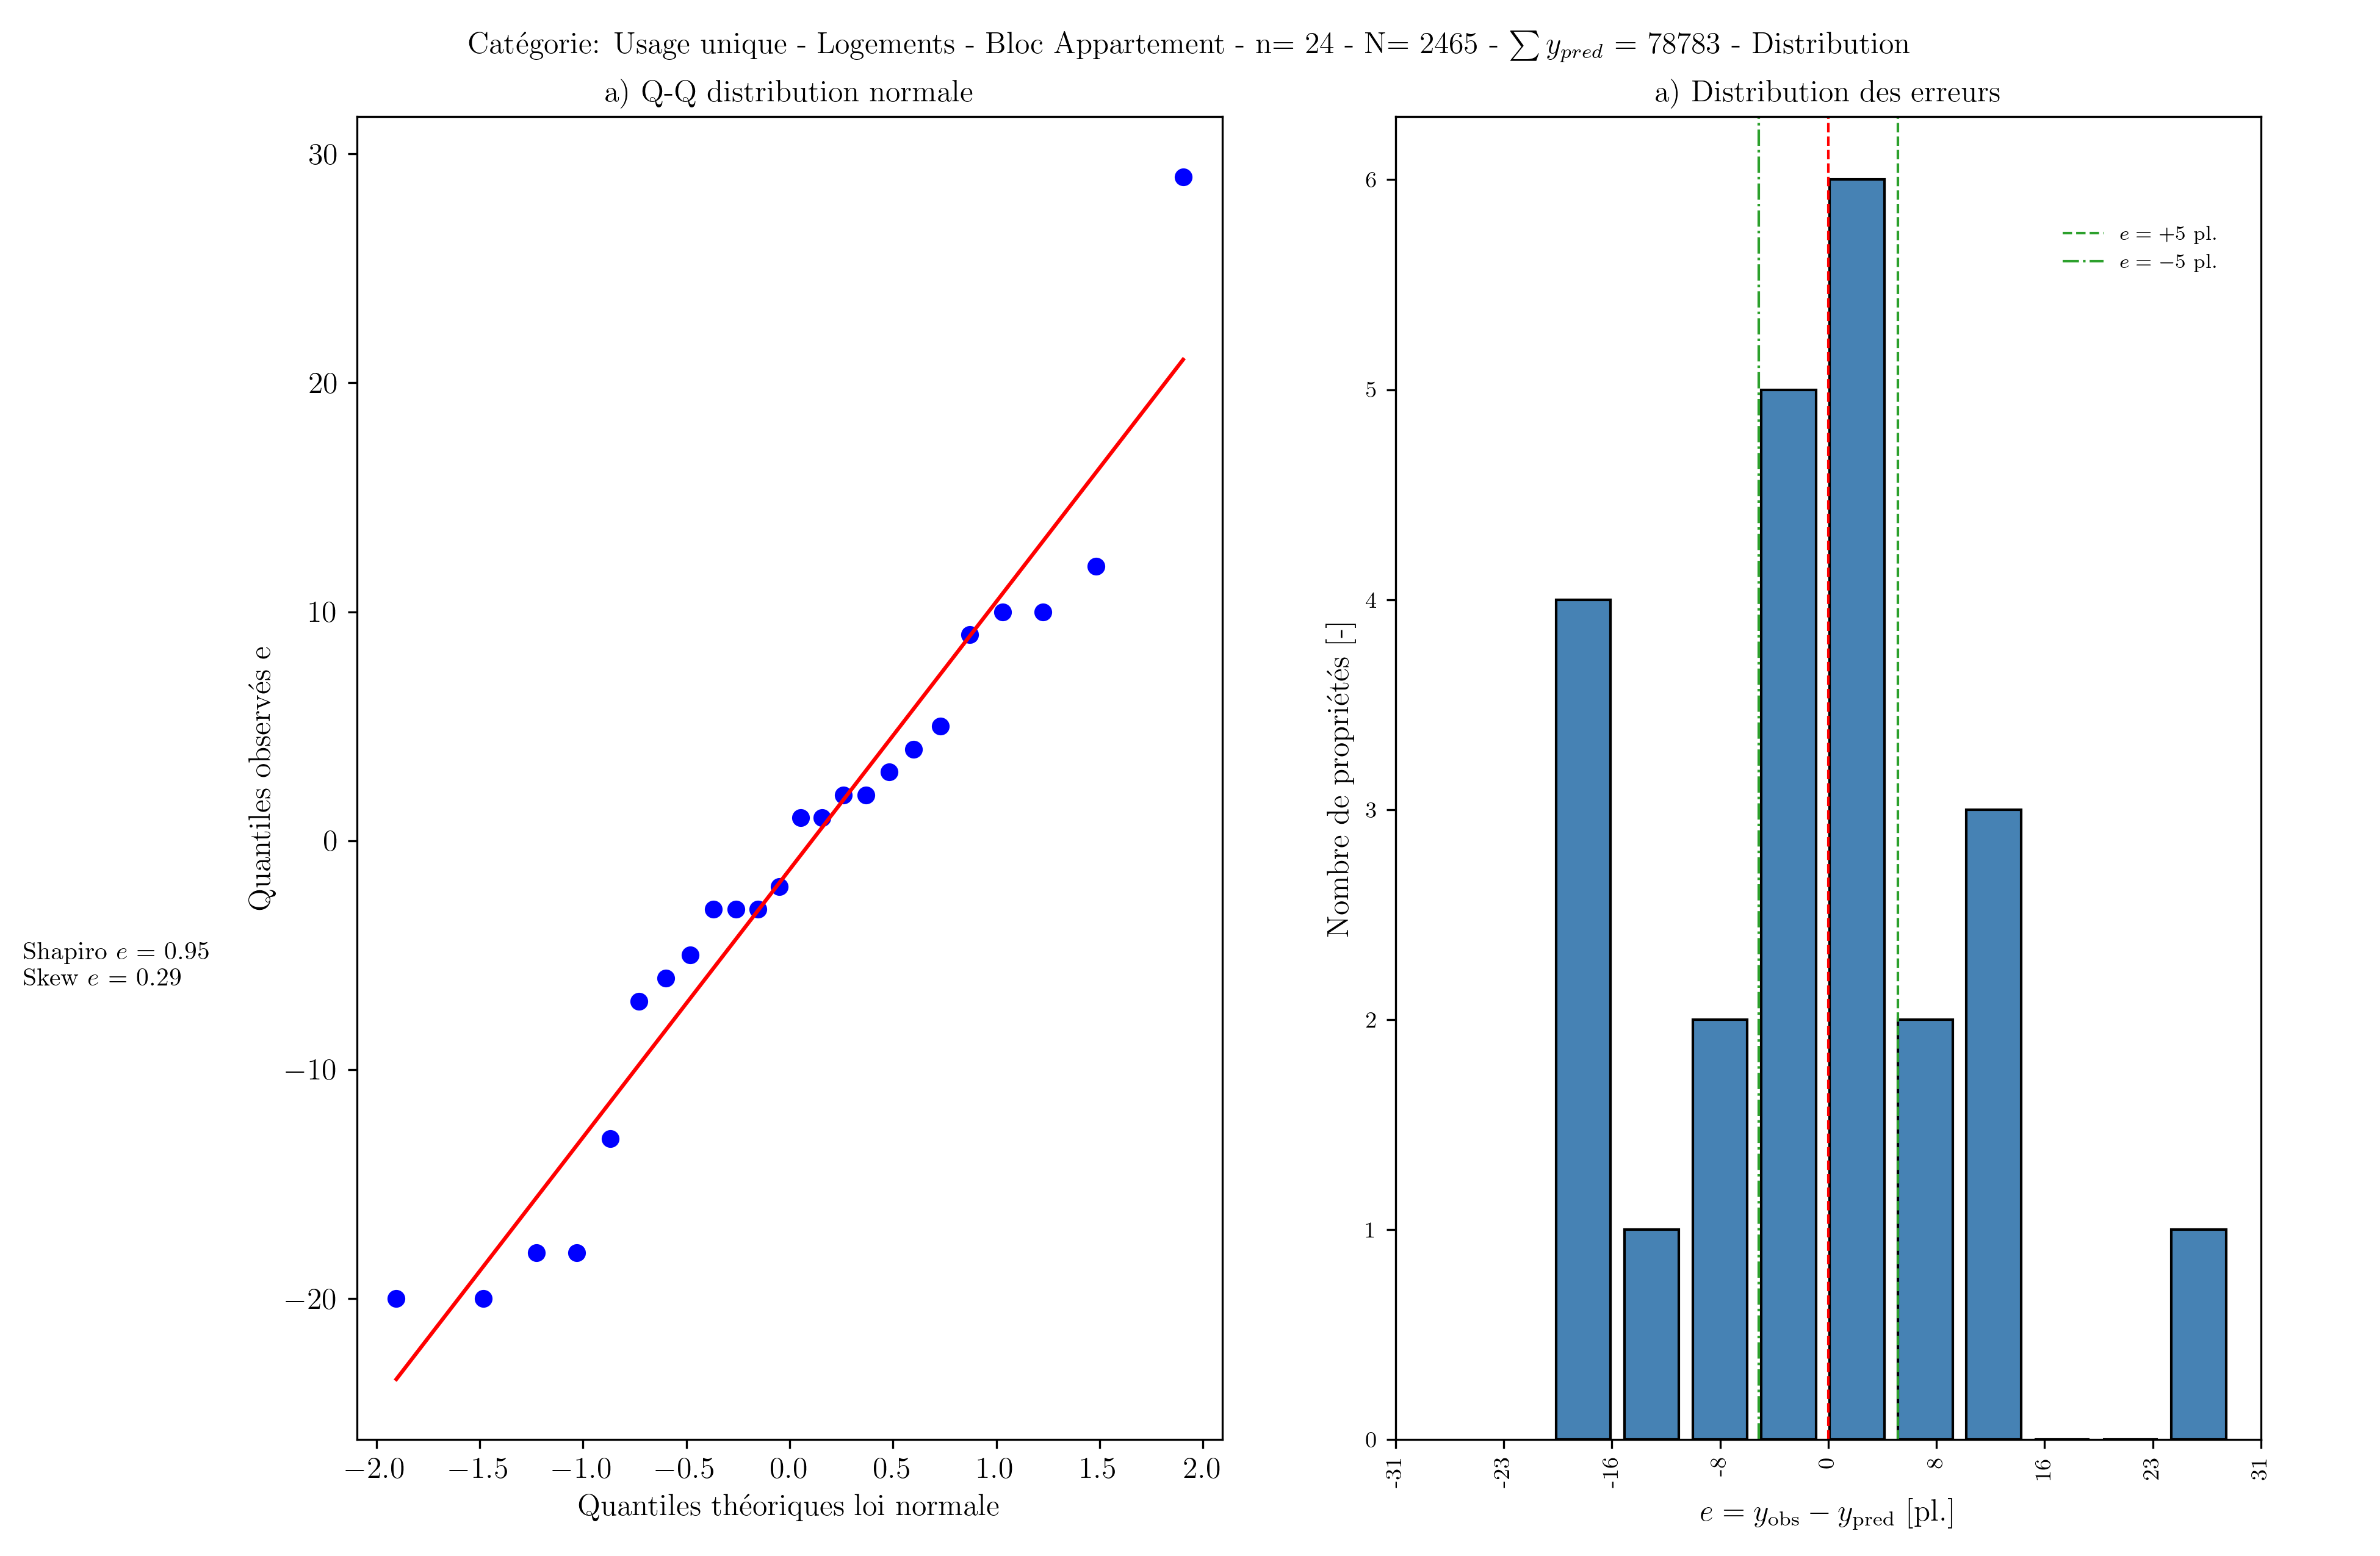
\includegraphics[width=1\linewidth]{images/int_erreur_44_se_5_pe_20_c.png}
        \caption{Distribution et normalité des erreurs pour les grands immeubles résidentiels}
        \label{fig:dist-erreur-norm-log-bloc}
    \end{figure}
    \begin{figure}[H]
        \centering
        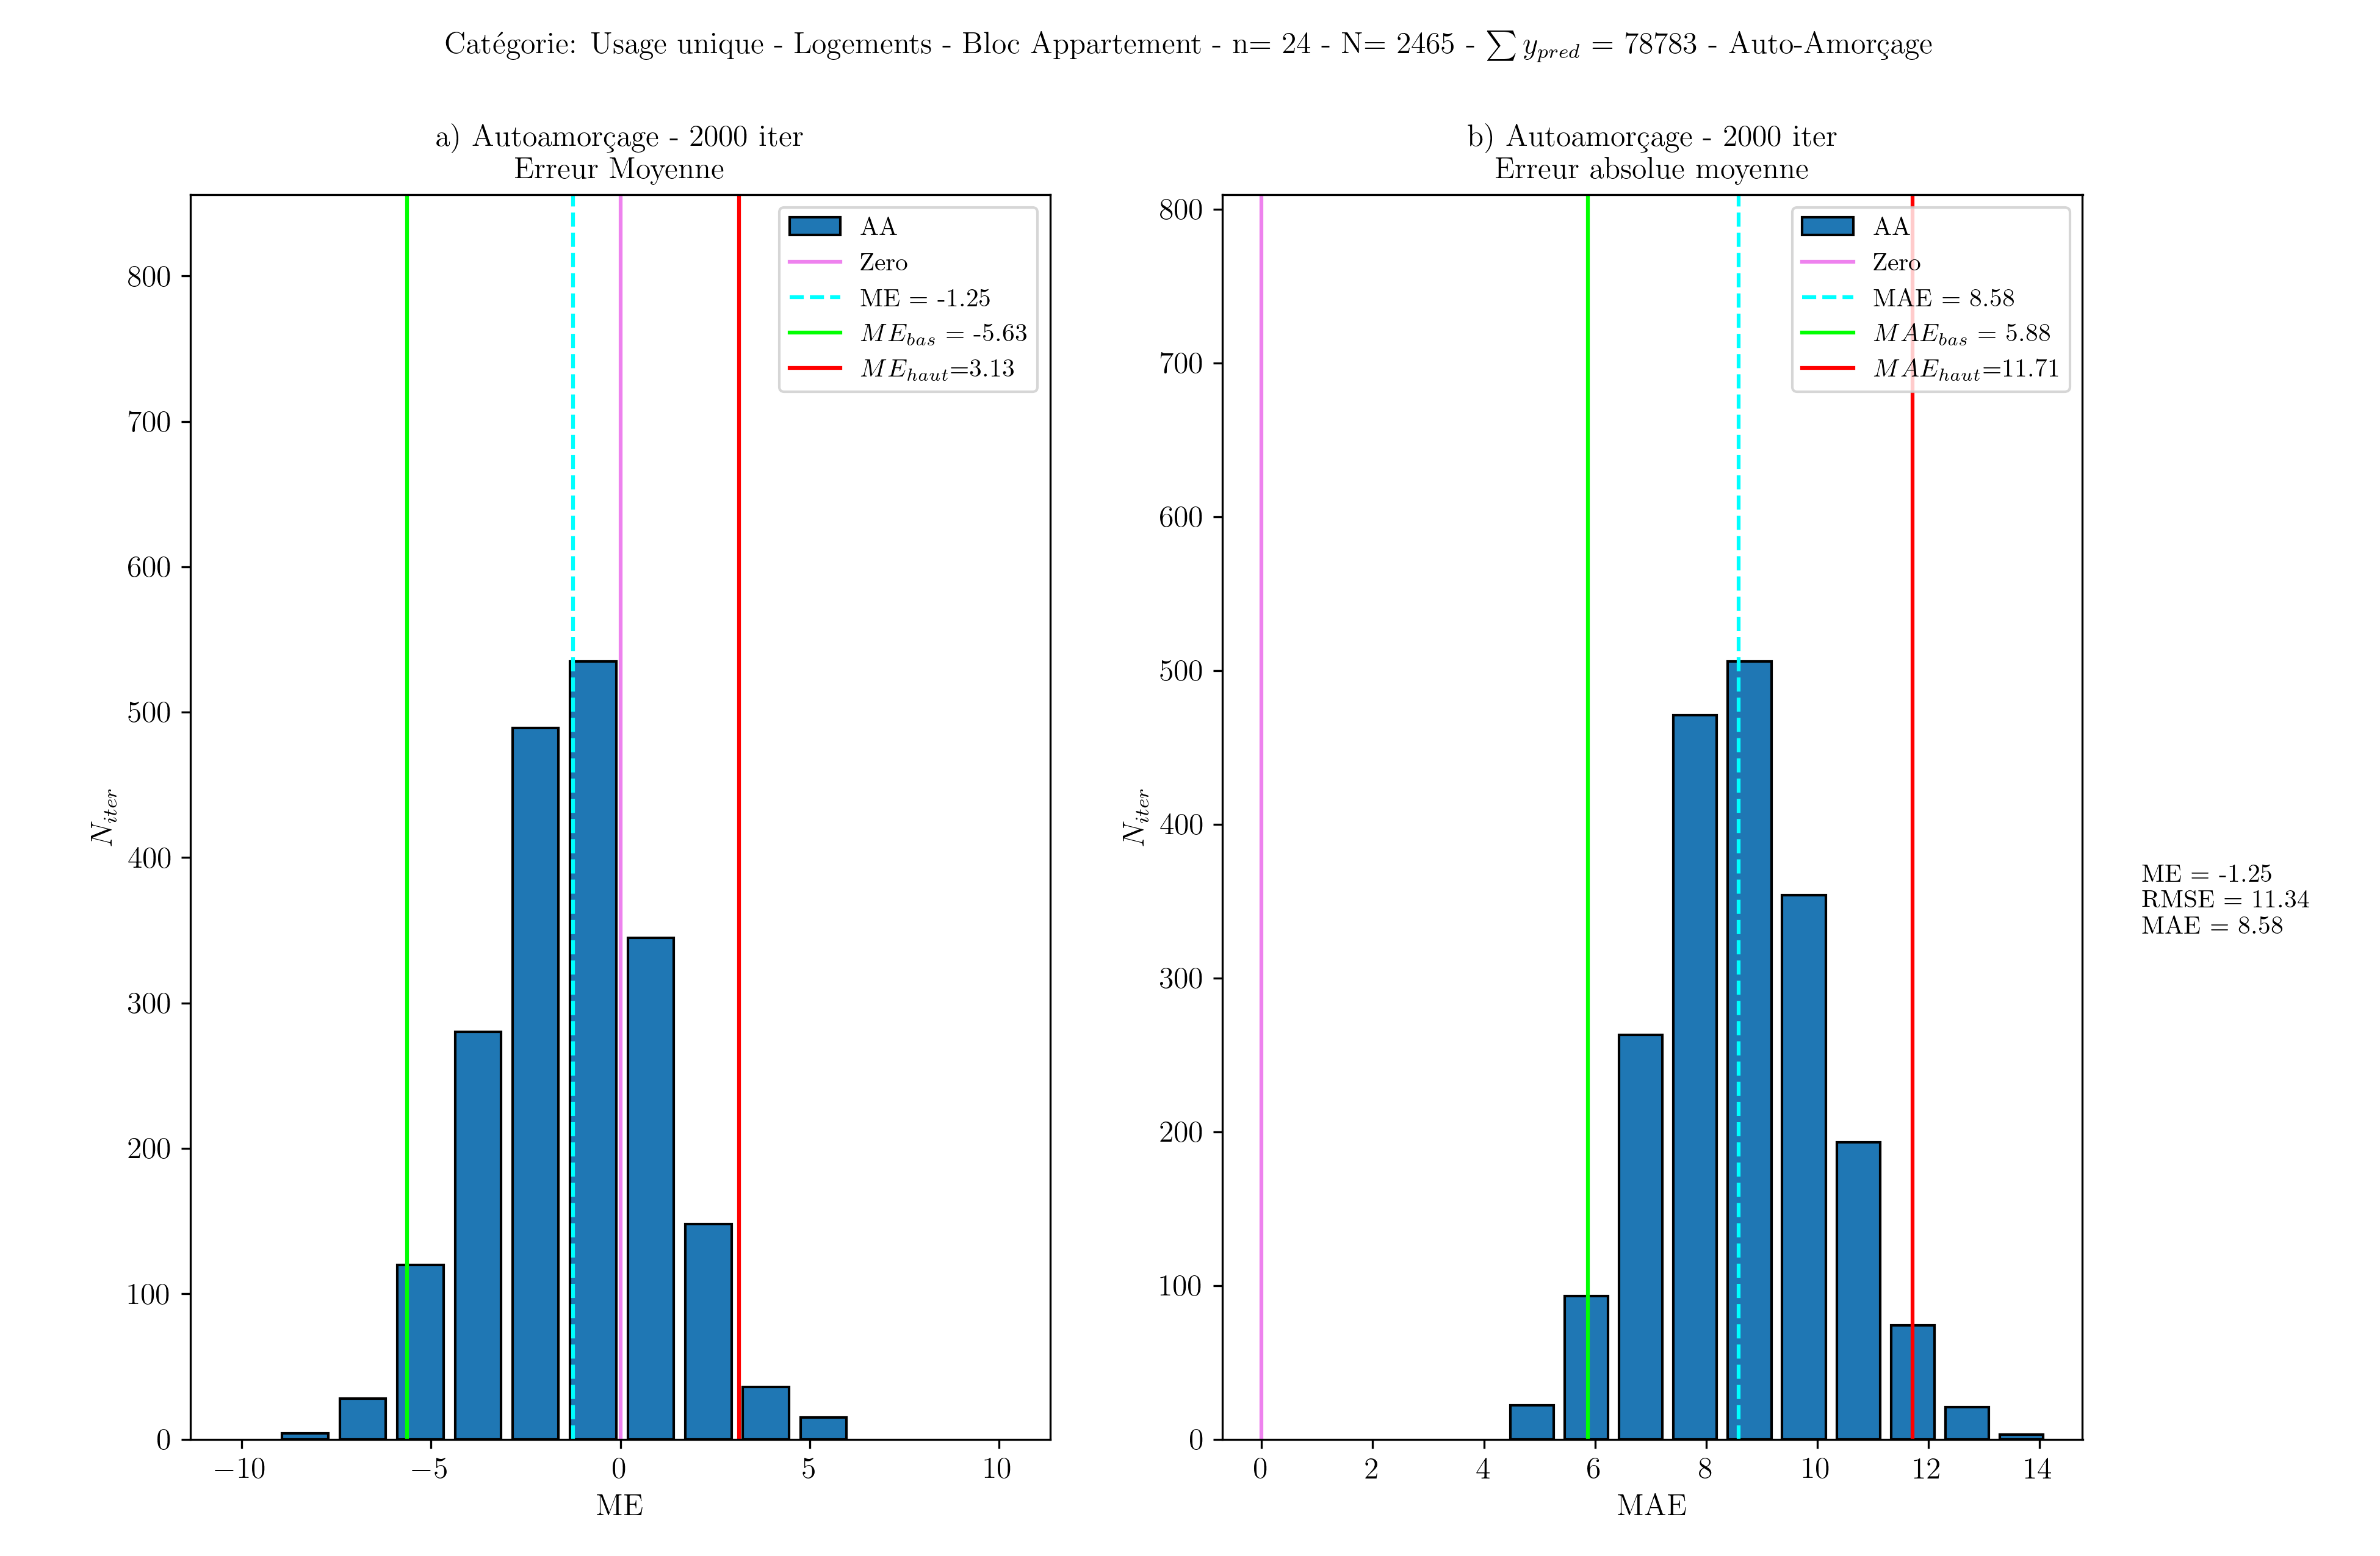
\includegraphics[width=1\linewidth]{images/int_erreur_44_se_5_pe_20_d.png}
        \caption{Distribution des métriques d'erreur après auto-amorçage pour les grands immeubles résidentiels}
        \label{fig:auto-amor-log-bloc}
    \end{figure}
    %\begin{figure}[H]
    %    \centering
    %    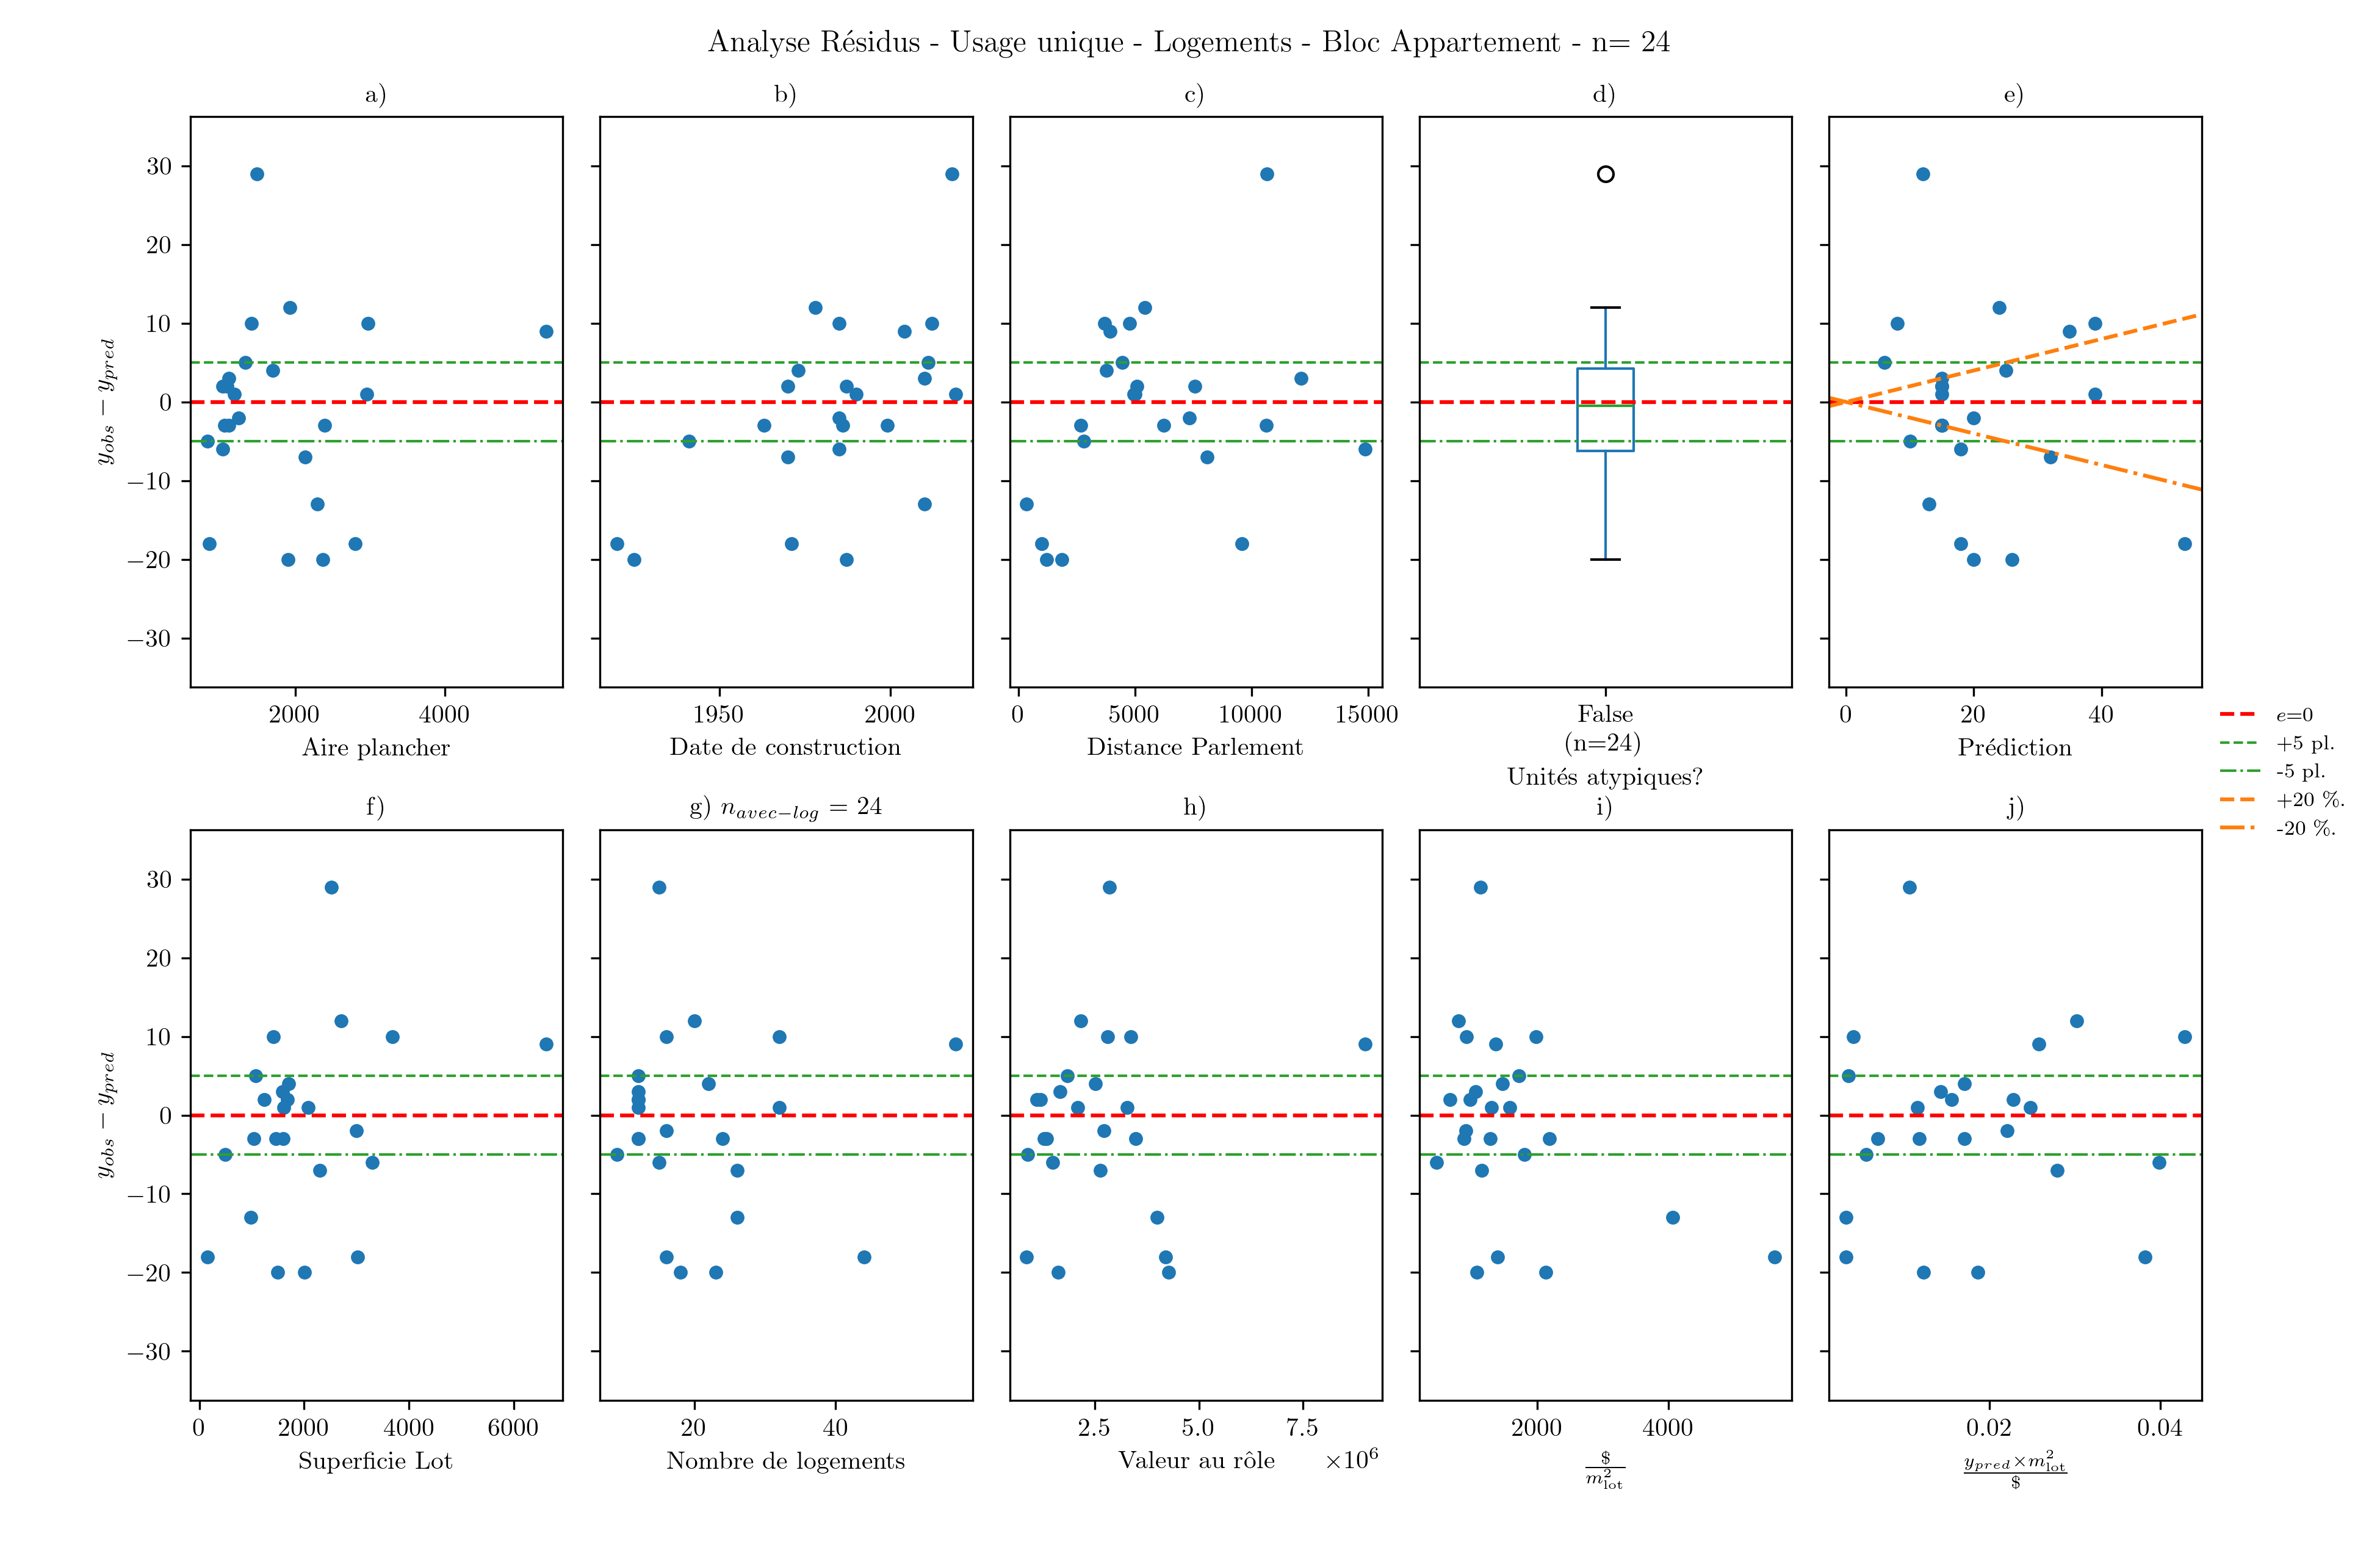
\includegraphics[scale=0.7]{images/ana_res_44_se_5_pe_20.png}
    %    \caption{Analyse des résidus la prédiction pour les grands immeubles résidentiels}
    %    \label{fig:ana-residu-log-bloc}
    %\end{figure}
    \begin{figure}[H]
        \centering
        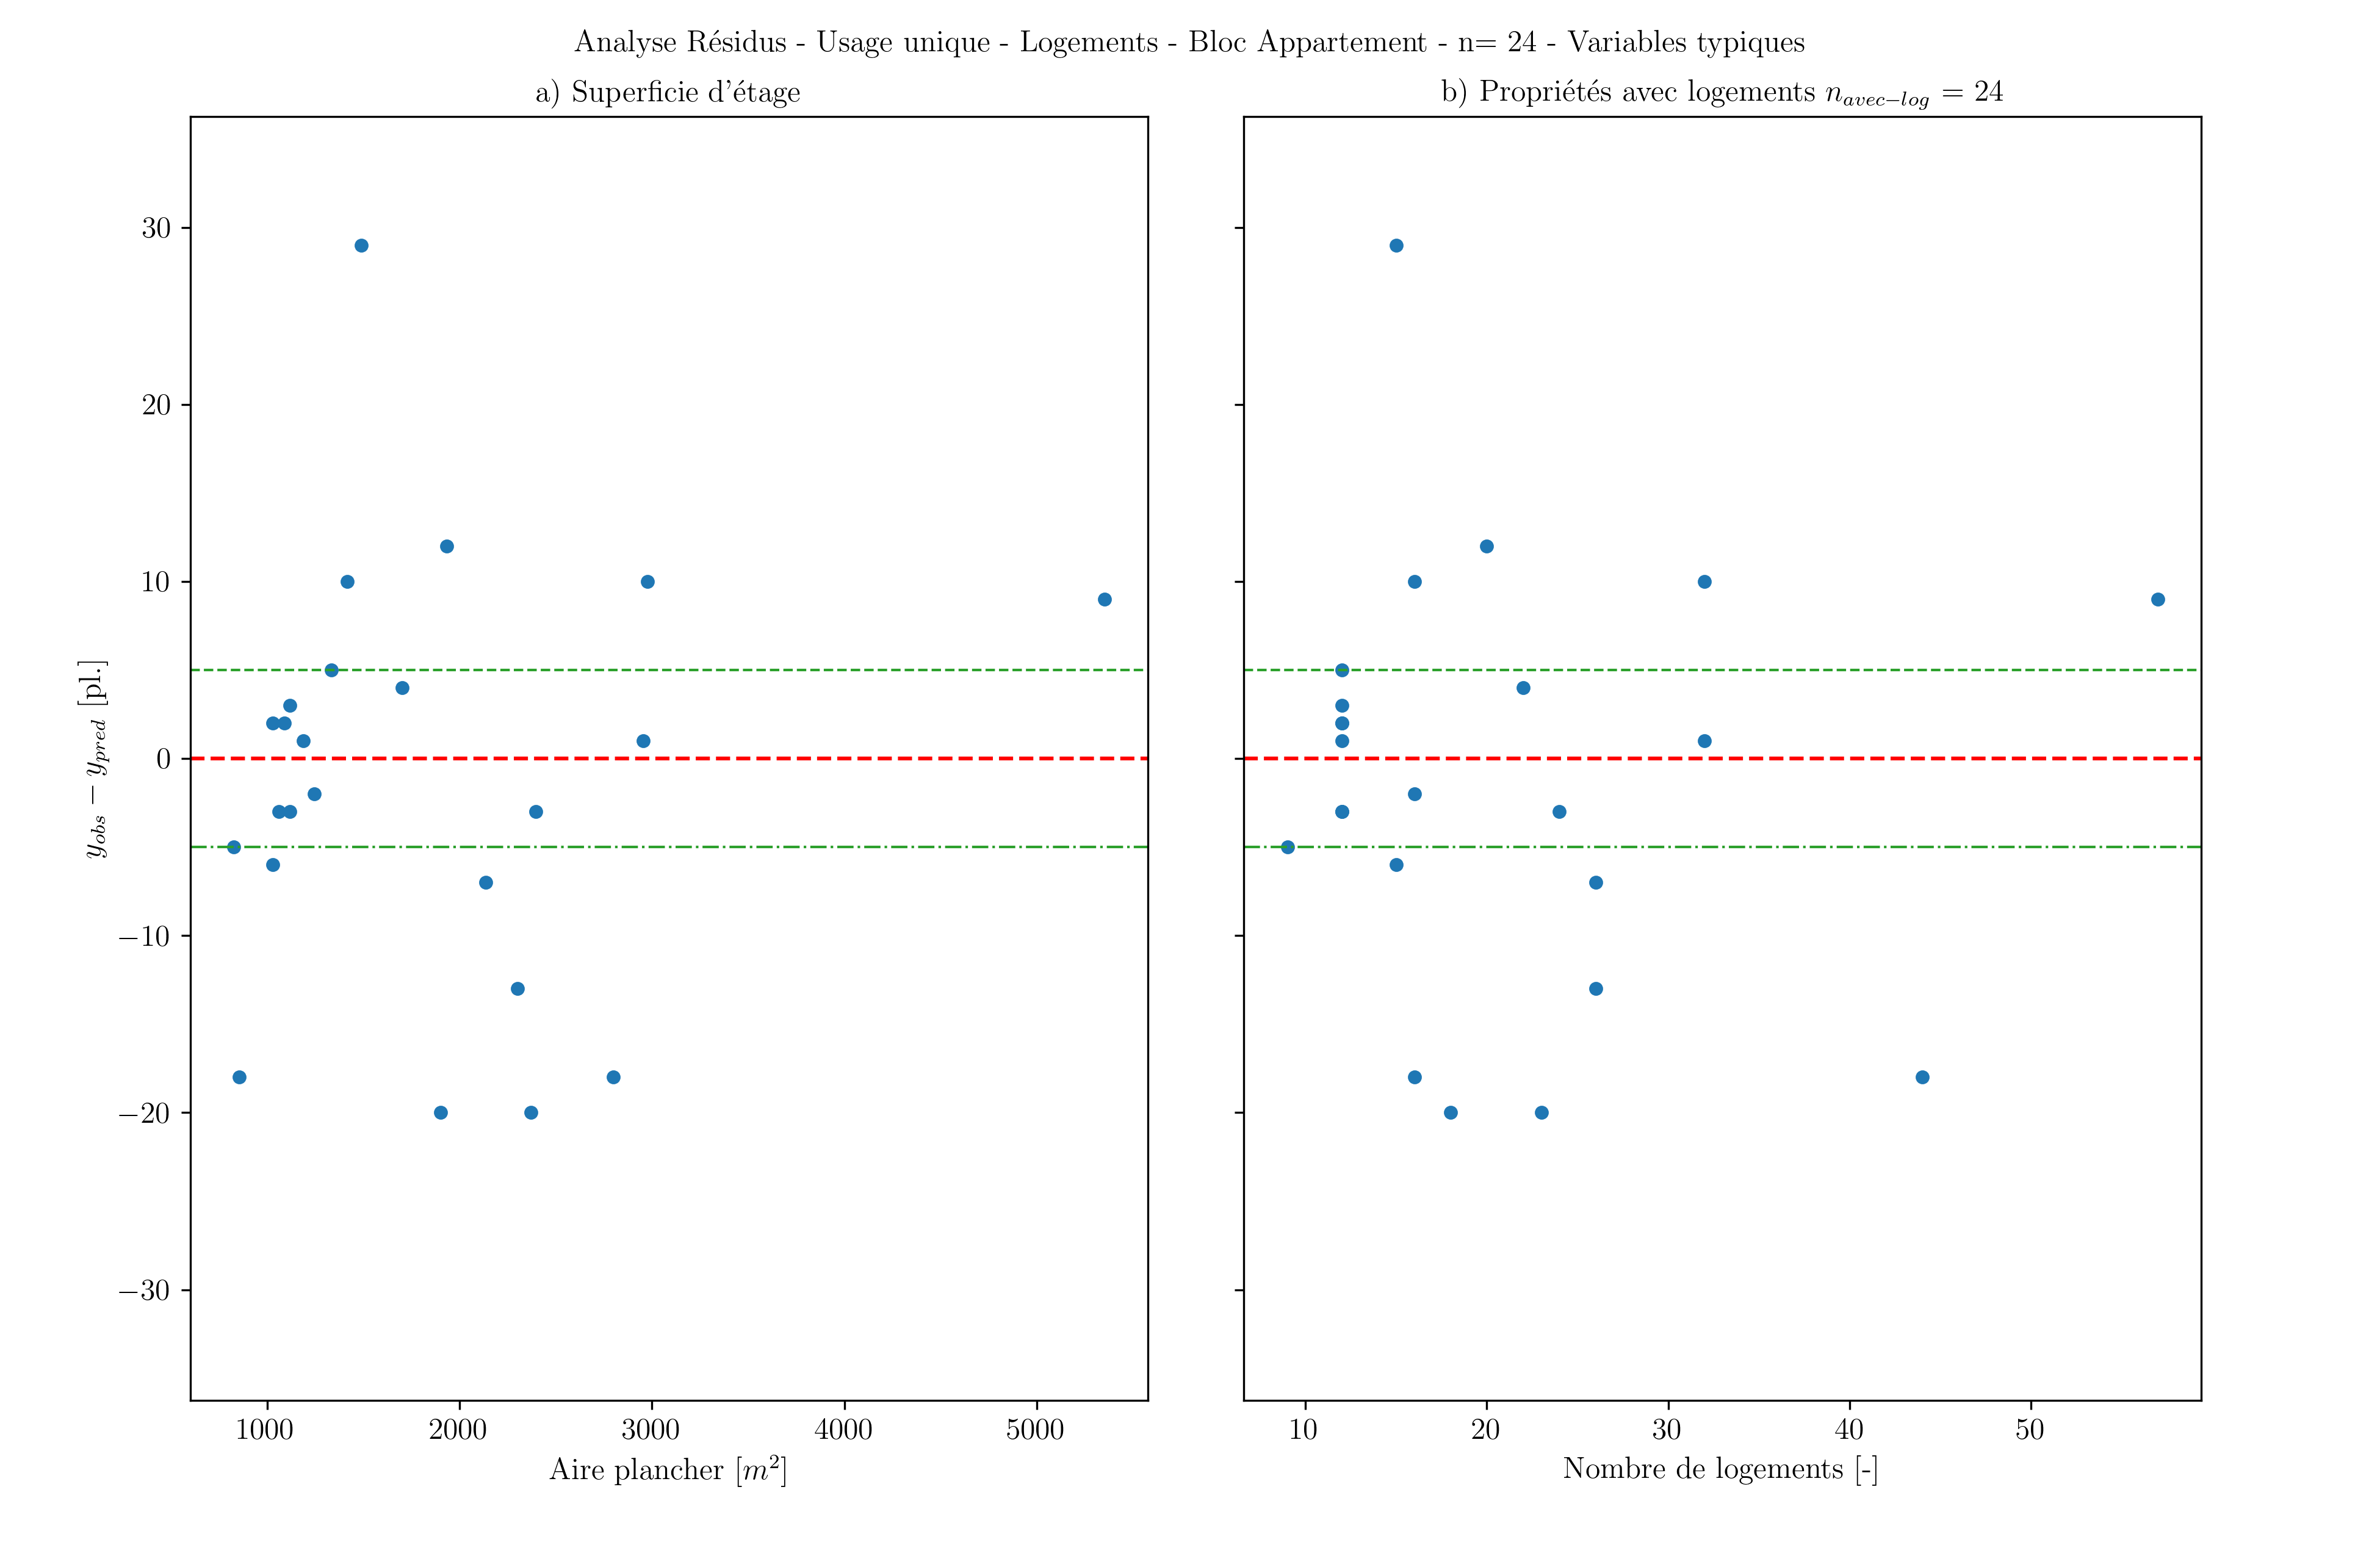
\includegraphics[width=1\linewidth]{images/ana_res_44_se_5_pe_20_a.png}
        \caption{Analyse des résidus en fonction des propriétés de construction pour les grands immeubles résidentiels}
        \label{fig:ana-res-prop-phys-log-bloc}
    \end{figure}
    \begin{figure}[H]
        \centering
        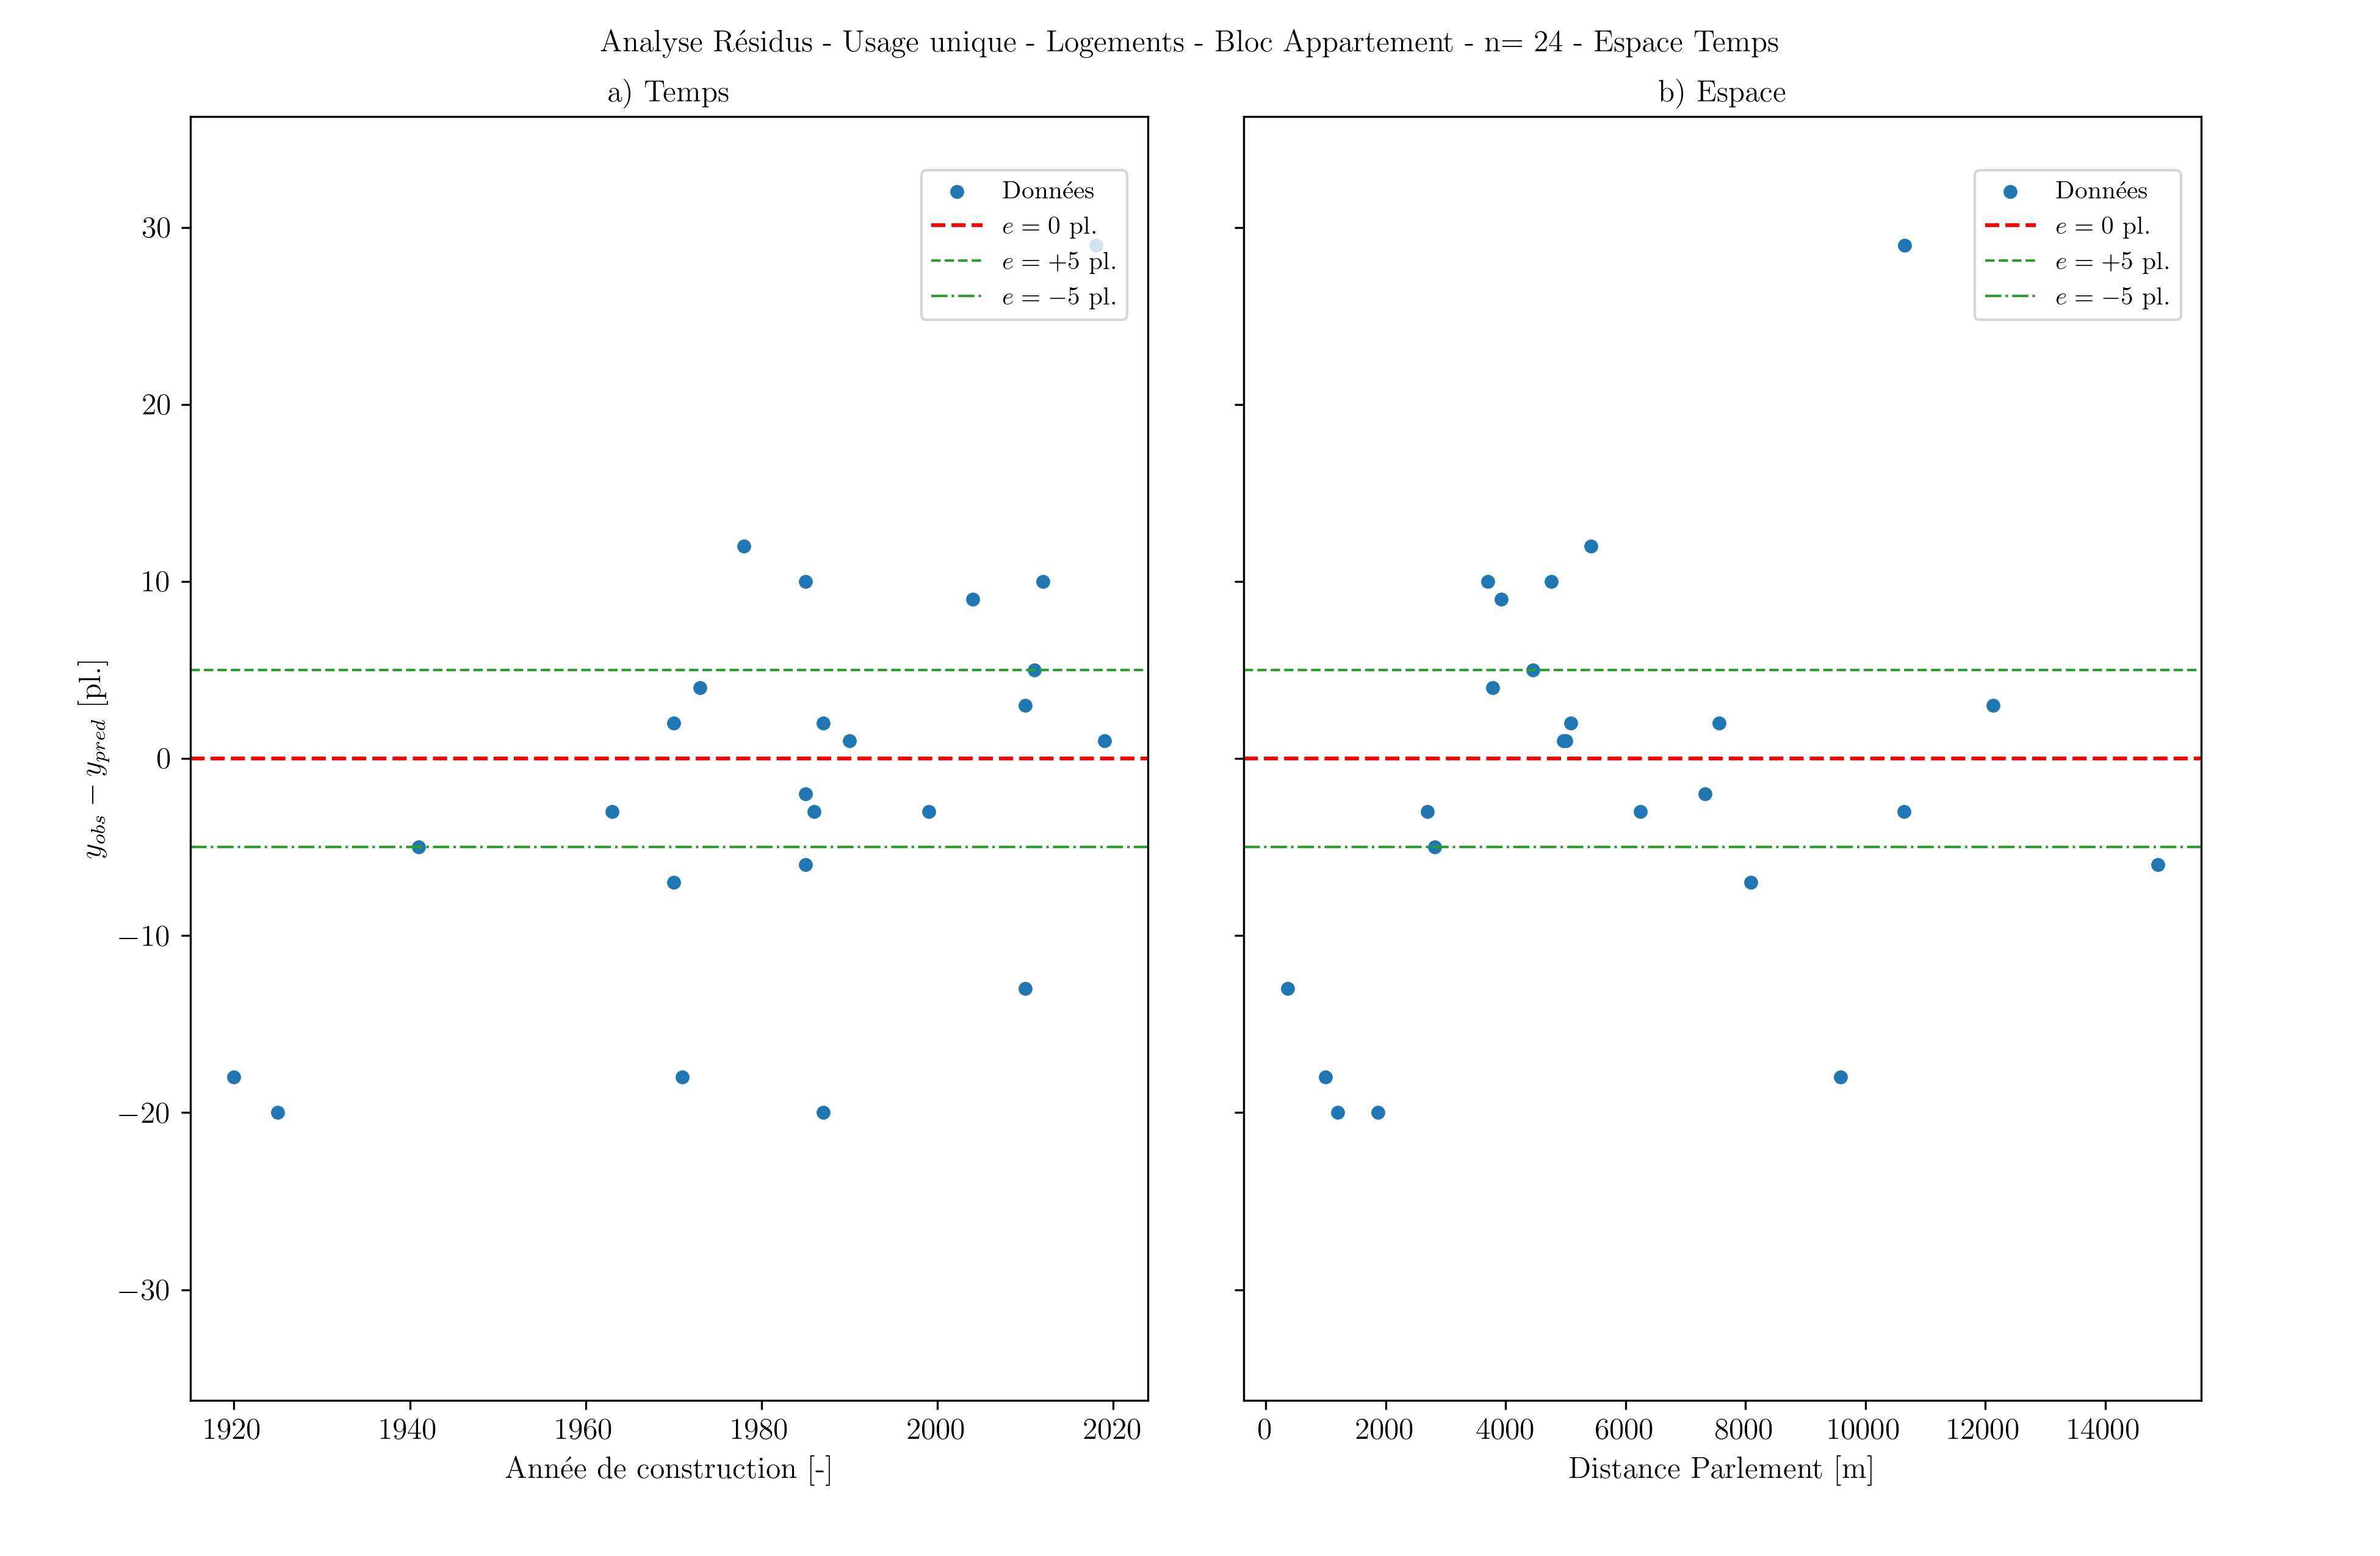
\includegraphics[width=1\linewidth]{images/ana_res_44_se_5_pe_20_b.png}
        \caption{Analyse des résidus en fonction de l'espace et de l'époque de construction pour les grands immeubles résidentiels}
        \label{fig:ana-res-esp-temps-log-bloc}
    \end{figure}
    \begin{figure}[H]
        \centering
        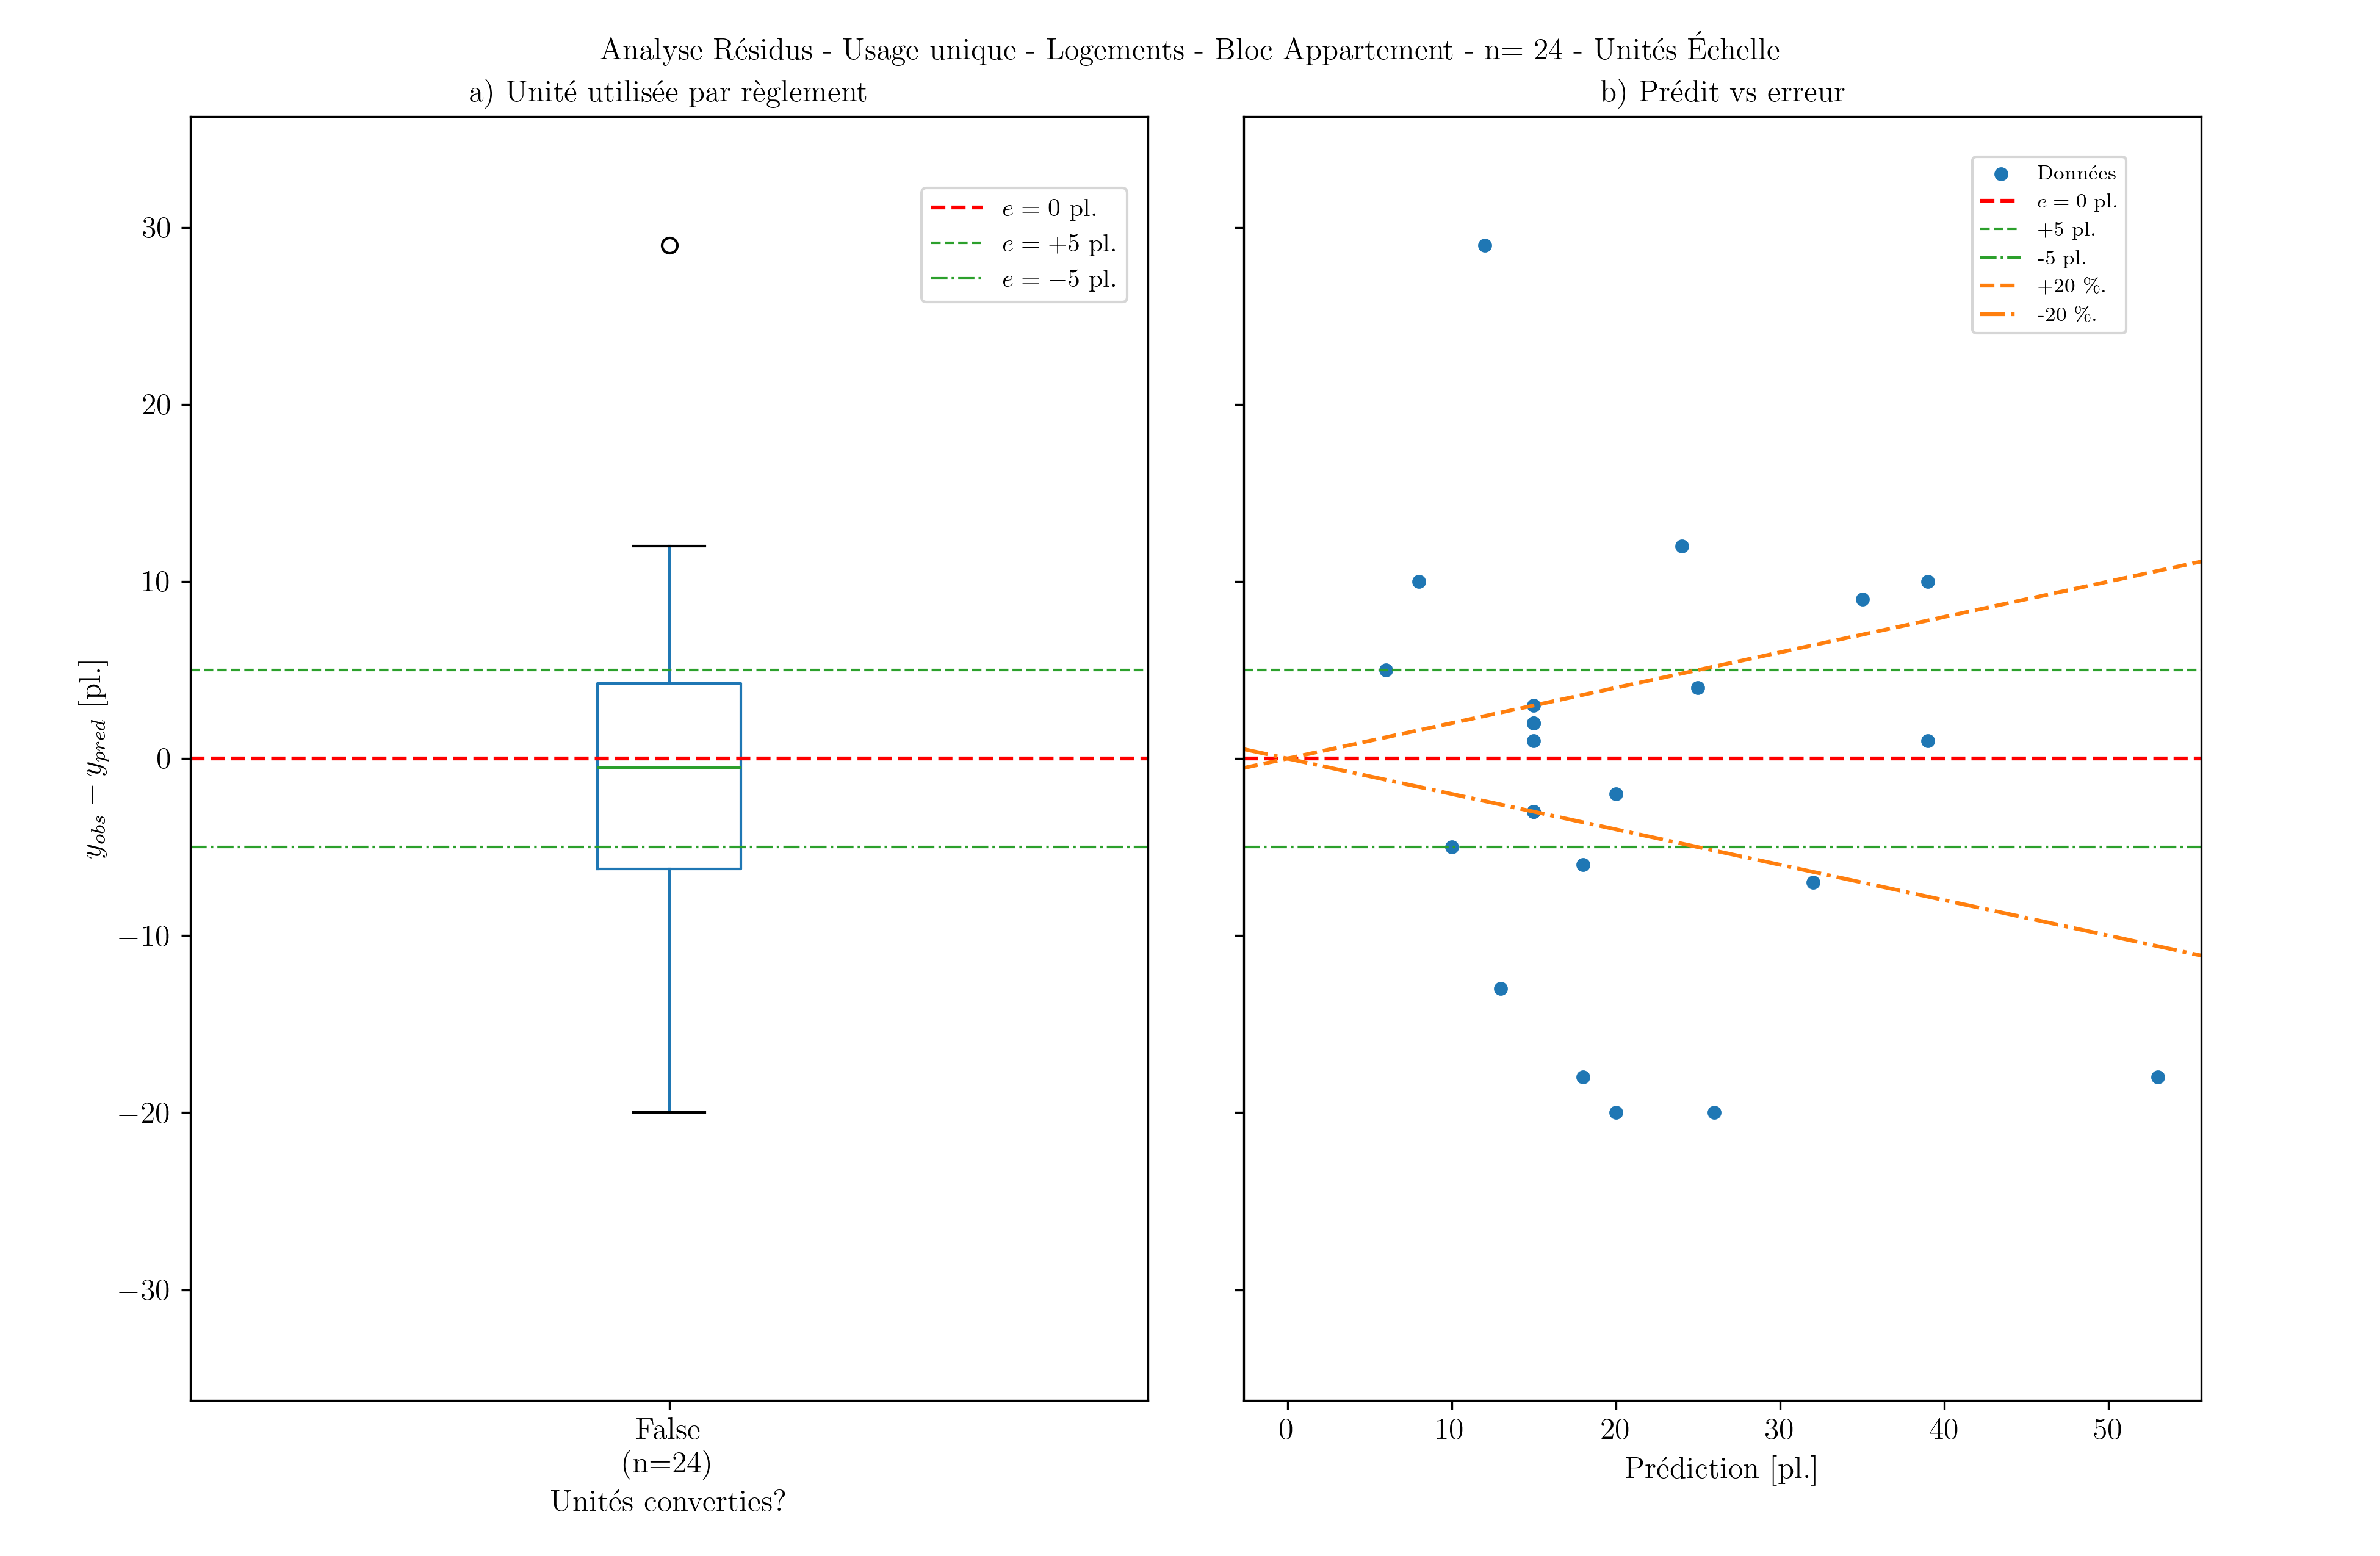
\includegraphics[width=1\linewidth]{images/ana_res_44_se_5_pe_20_c.png}
        \caption{Analyse des résidus en fonction de la prédiction et des unités de formulation pour les grands immeubles résidentiels}
        \label{fig:ana-res-unit-pred-log-bloc}
    \end{figure}
    \begin{figure}[H]
        \centering
        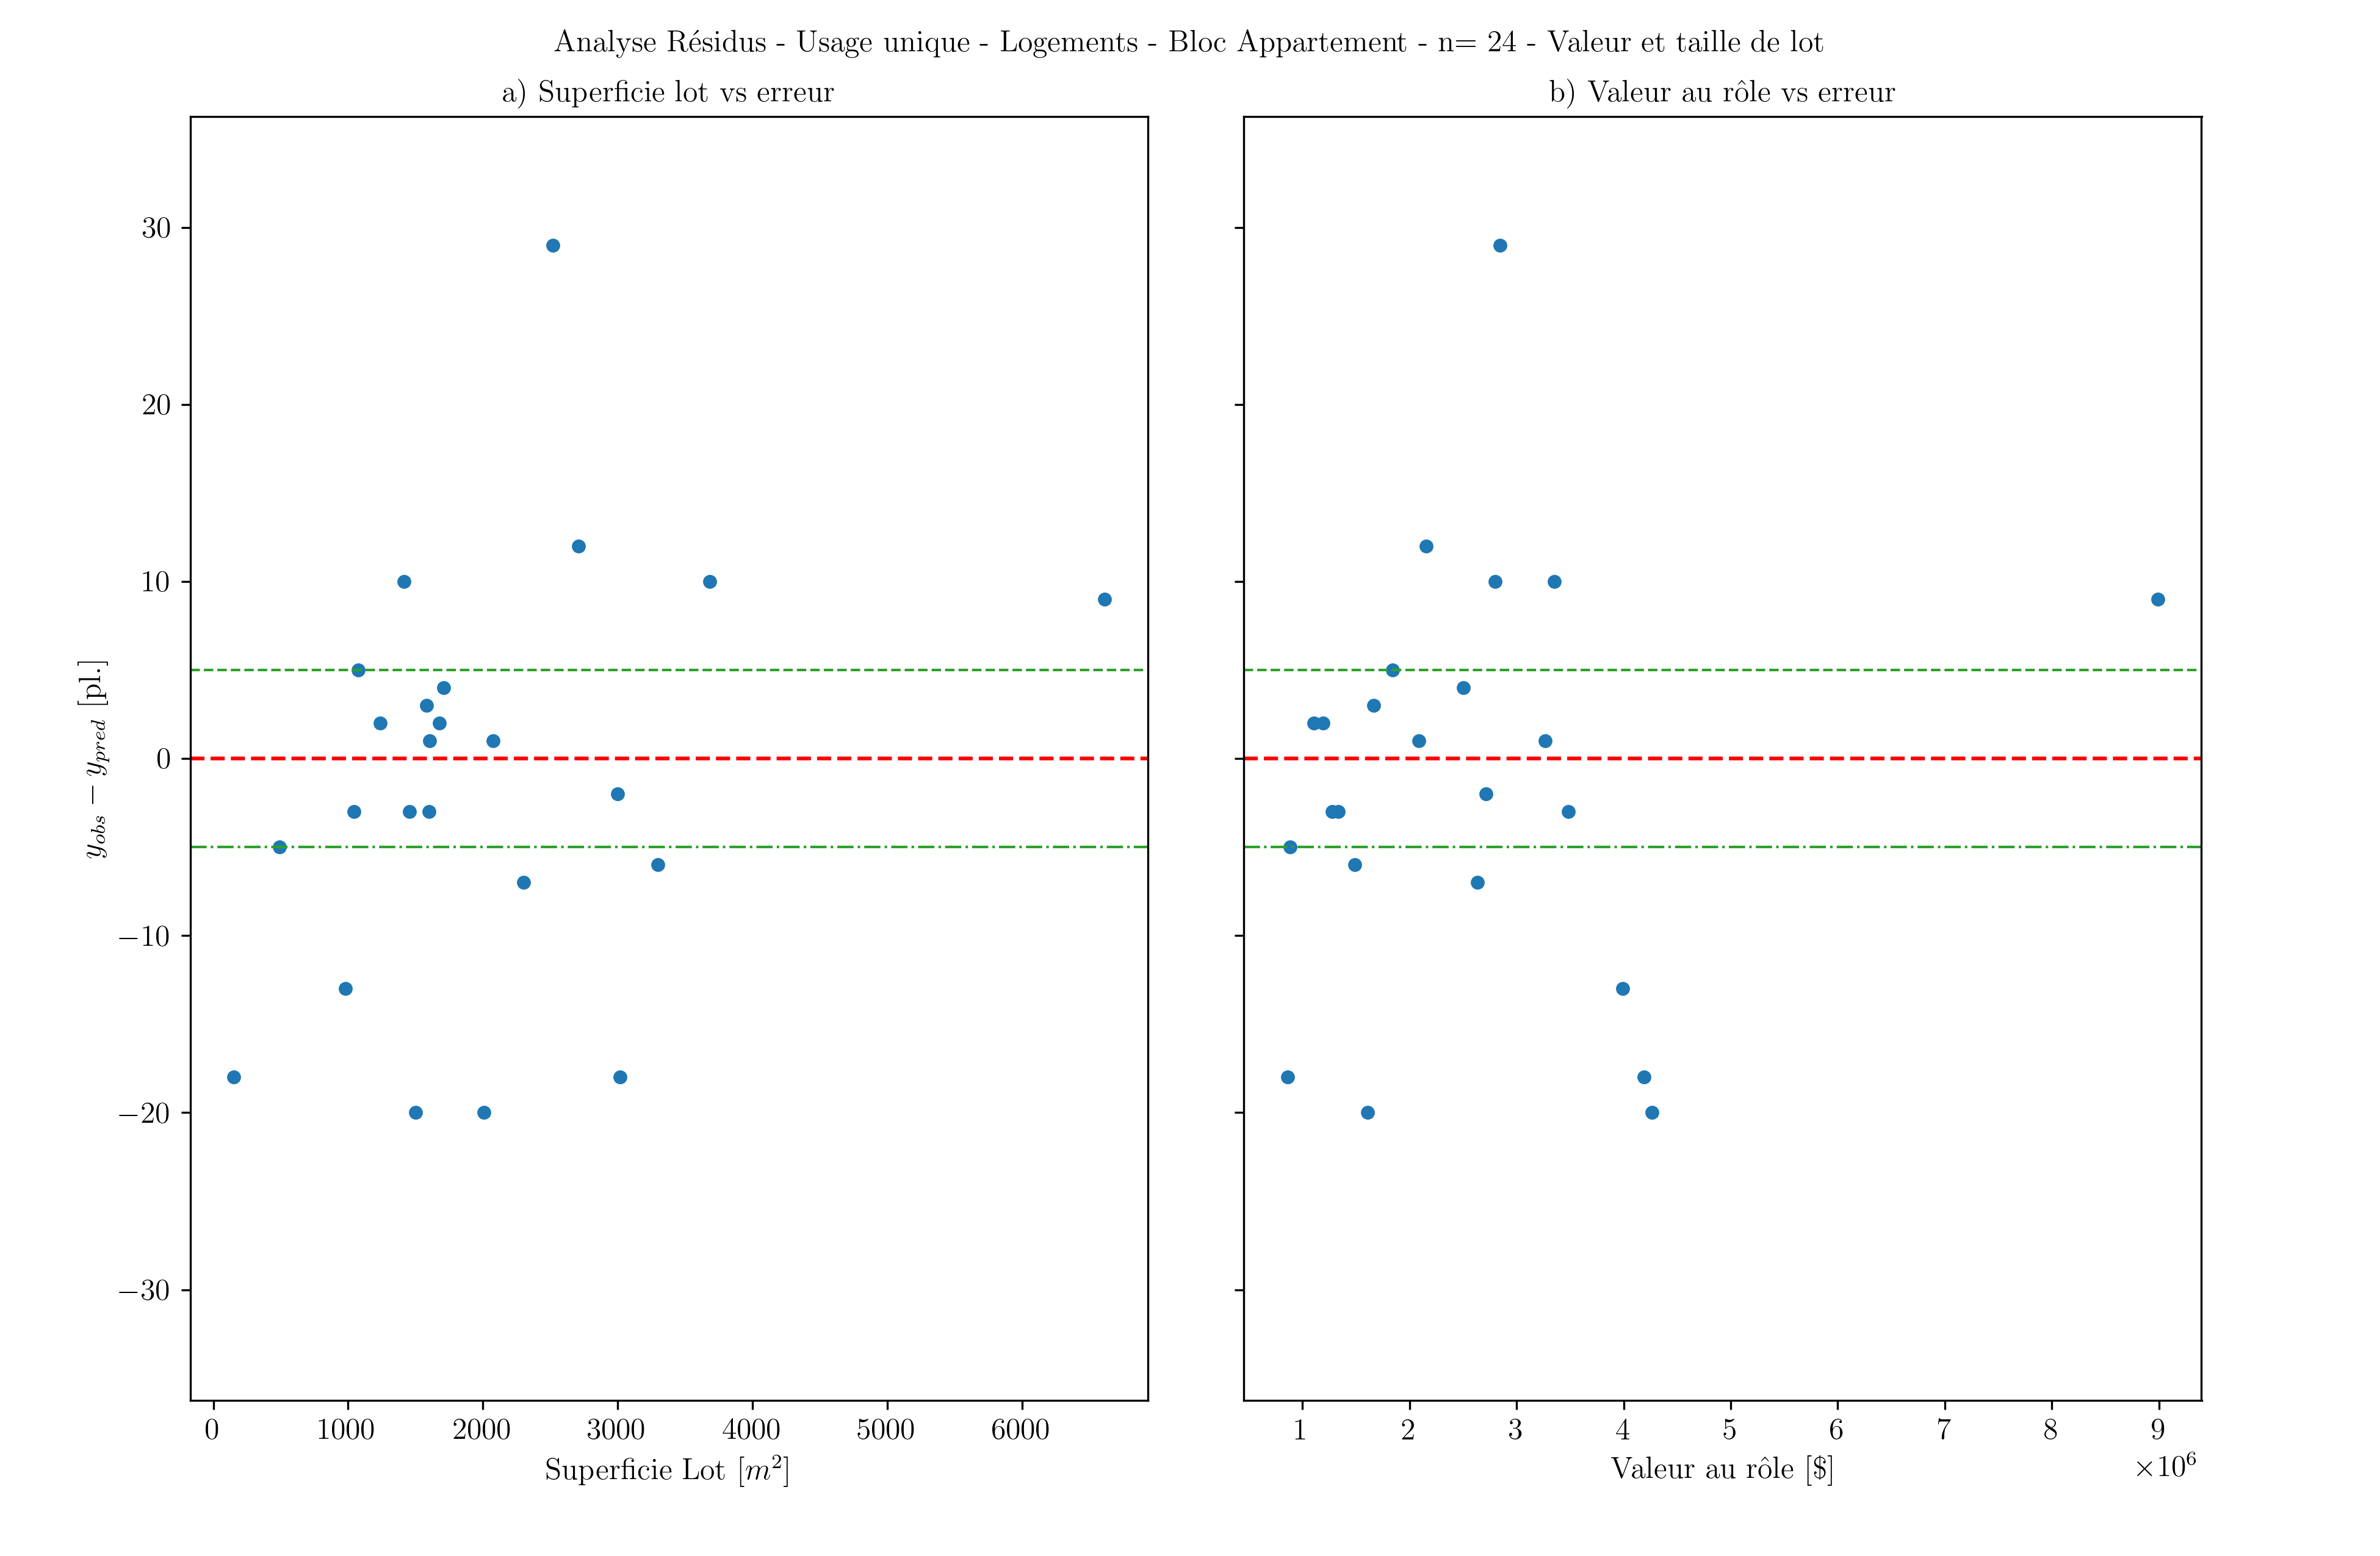
\includegraphics[width=1\linewidth]{images/ana_res_44_se_5_pe_20_d.png}
        \caption{Analyse des résidus en fonction de la superficie du lot et de la valeur pour les grands immeubles résidentiels}
        \label{fig:ana-res-sup-val-log-bloc}
    \end{figure}
    \begin{figure}[H]
        \centering
        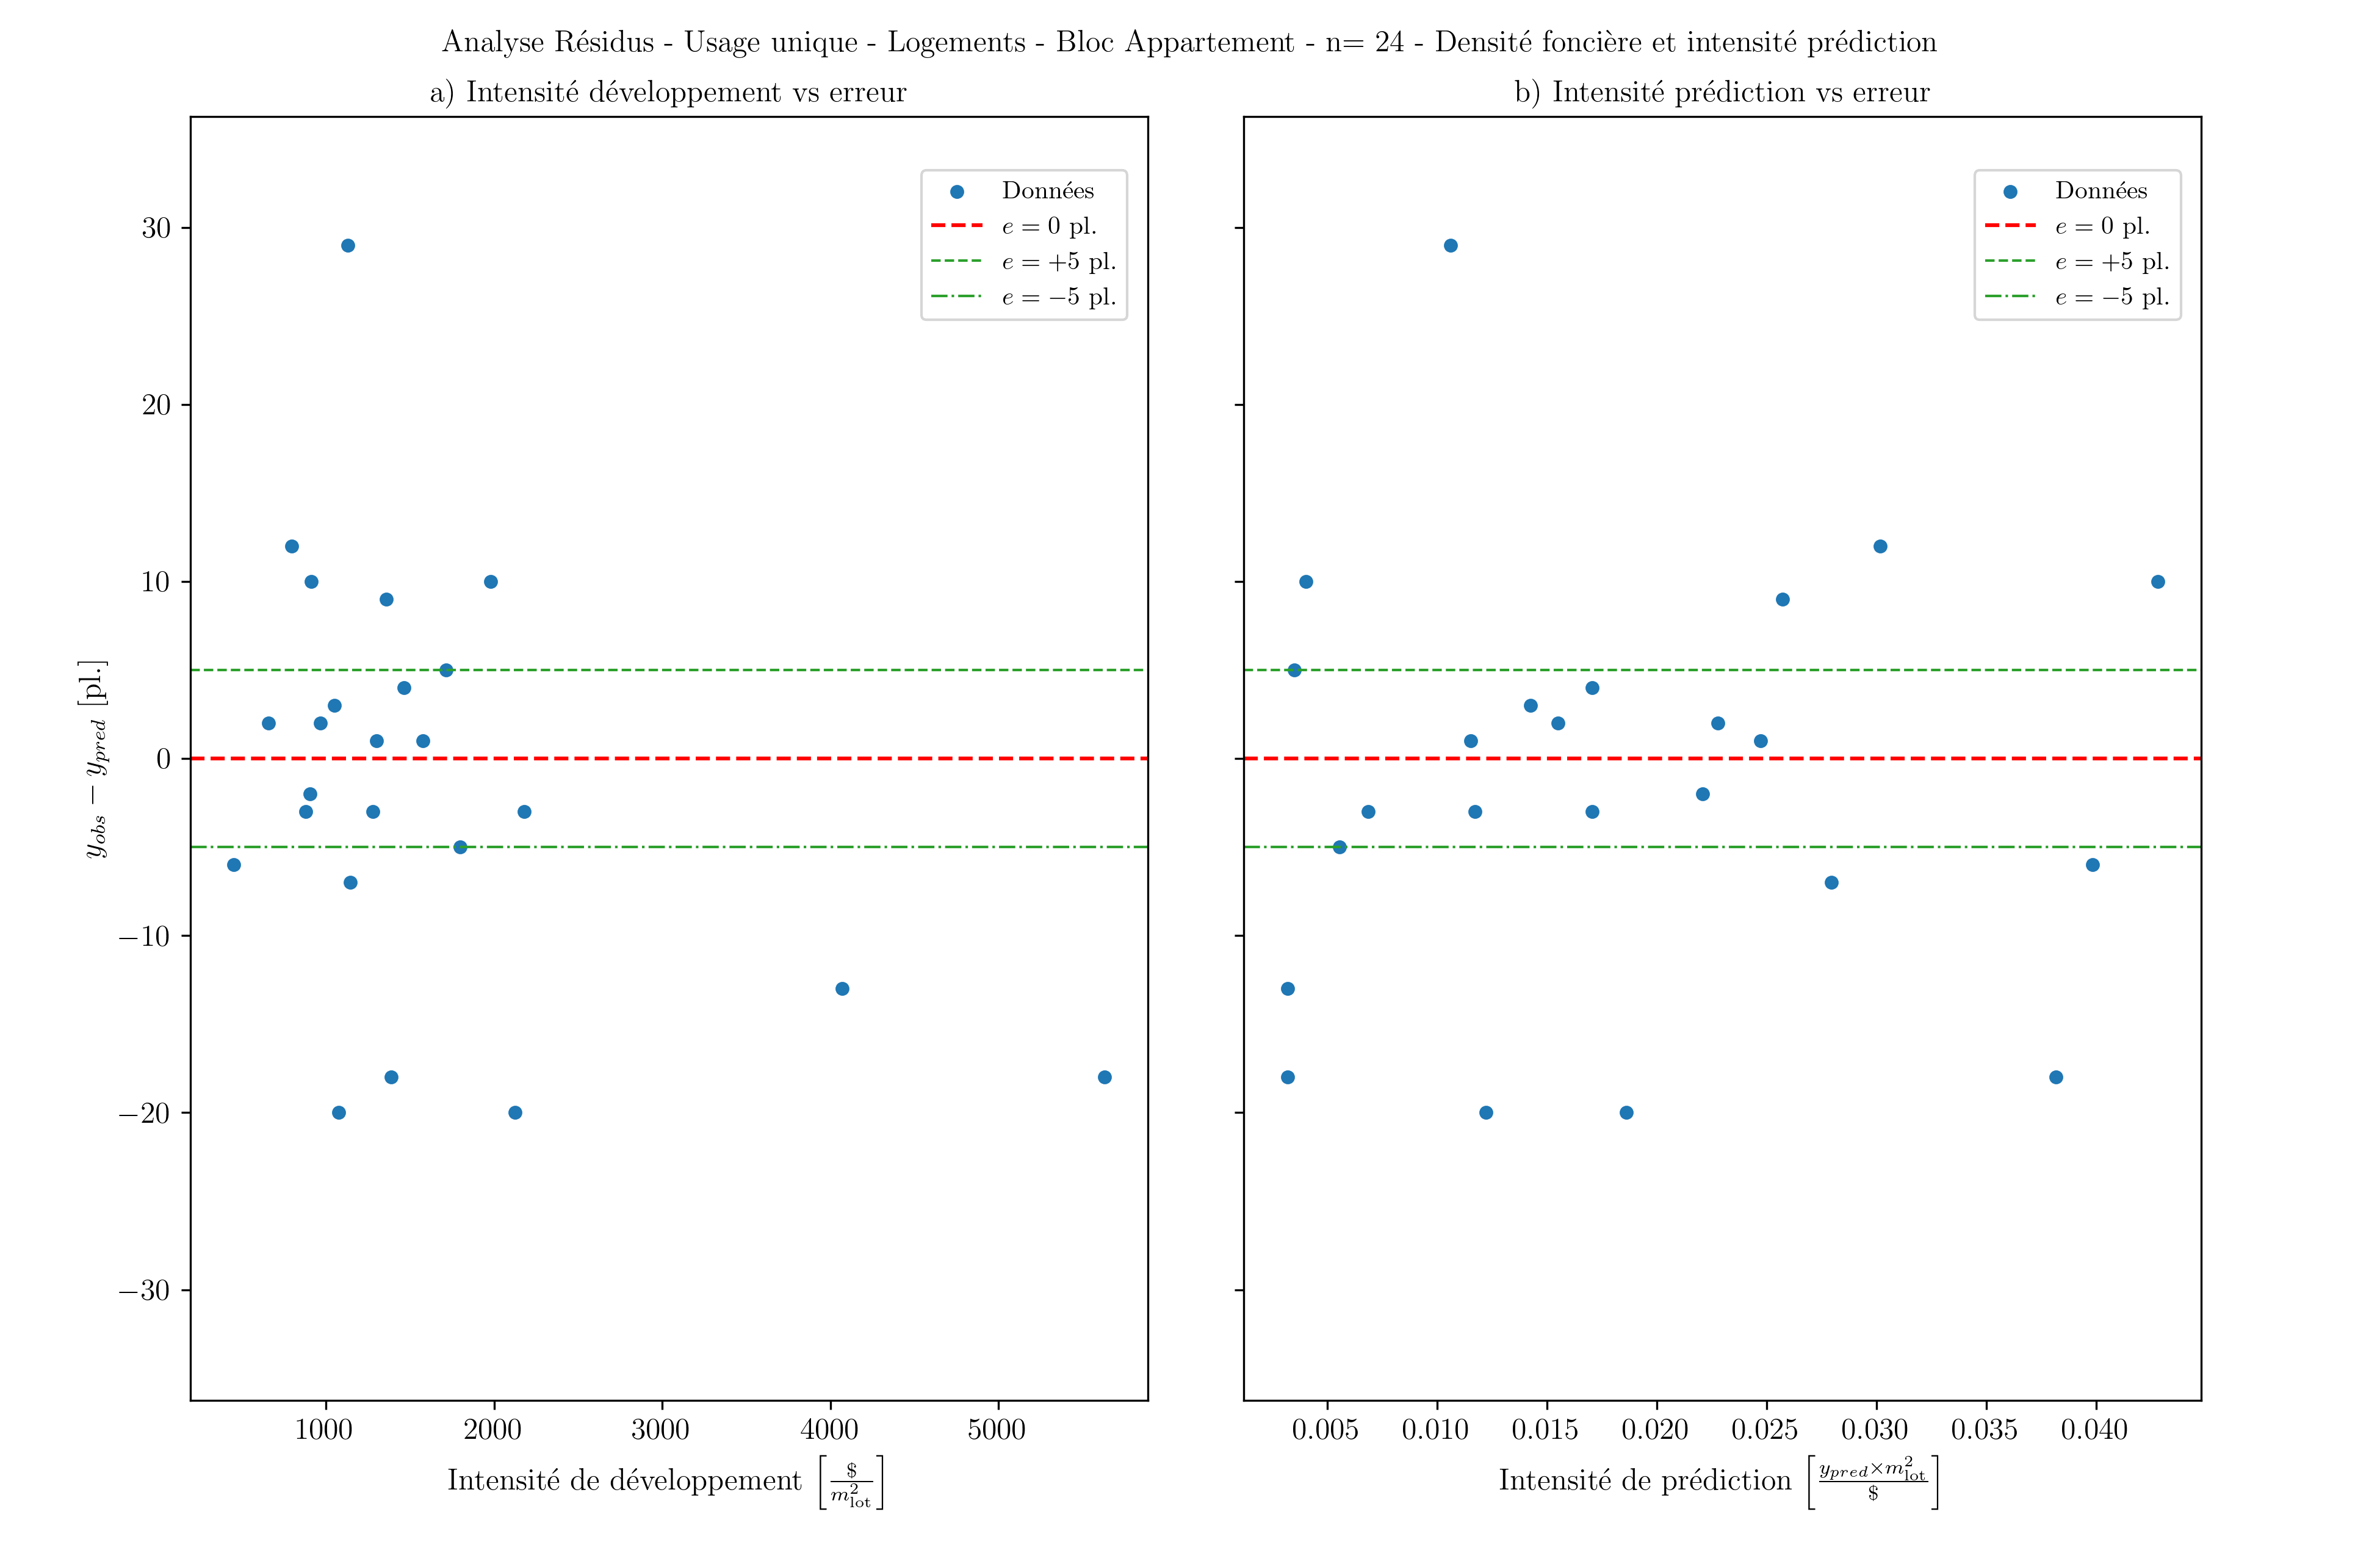
\includegraphics[width=1\linewidth]{images/ana_res_44_se_5_pe_20_e.png}
        \caption{Analyse des résidus en fonction de l'intensité de développement et l'intensité de prédiction pour les grands immeubles résidentiels}
        \label{fig:ana-res-intens-log-bloc}
    \end{figure}
\end{landscape}
\subsection{Commercial}

Trente lots commerciaux ont été échantillonnés pour valider la performance du modèle. Une propriété dont l'utilisation est commerciale a une erreur de plus de 300 places. Cette propriété est un immeuble commercial construit dans les années 1970 et se trouve dans la zone industrielle de la Cité-Universitaire.  Un filtre pour les erreurs de plus de 75 places a été appliqué pour l'enlever pour le calcul des statistiques. Ce filtrage change la moyenne de la catégorie de $\bar{y}_{pred} = 55.6 $ à $\bar{y}_{pred} = 46.3 $.  La valeur moyenne observée $\bar{y}_{obs}$ est 44.0.\par
La figure \ref{fig:ana-res-intens-comm}b montre une variable d'intensité (eq. \ref{eq:intensite-stat-pred}) qui semble être un bon indicateur pour identifier les valeurs aberrantes. Deux requêtes SQL ont été lancées à des seuils de 0.25 et 0.5. 61 et 10 lots respectivement ont été trouvés qui auraient un enjeu potentiel.  Au premier niveau de seuil, 18 des 61 propriétés étaient affectées au même règlement que la valeur aberrante. Il s'agit d'un des 5 règlements reliés au commerce de détail avec des niveaux variants de .025 places par mètre carré à 0.1 place par mètre carré pour la municipalité concernée. Une requête pour extraire la liste de propriétés potentiellement affectées de la base de données est donnée en annexe \ref{ann:requete-intensite-stat}.\par

La figure \ref{fig:comm-err-by-unit} montre l'erreur en fonction de l'unité de formulation du règlement. On constate que les prédictions faites avec une étape de conversion ont un biais moyen introduit. C'est particulièrement le cas pour les commerces liés à l'automobile. L'annexe \ref{ann:recerche-inv-par-unite} donne un exemple de requête pour extraire les propriétés par l'unité de formulation du règlement.\par

\begin{landscape}
    \begin{figure}[H]
        \centering
        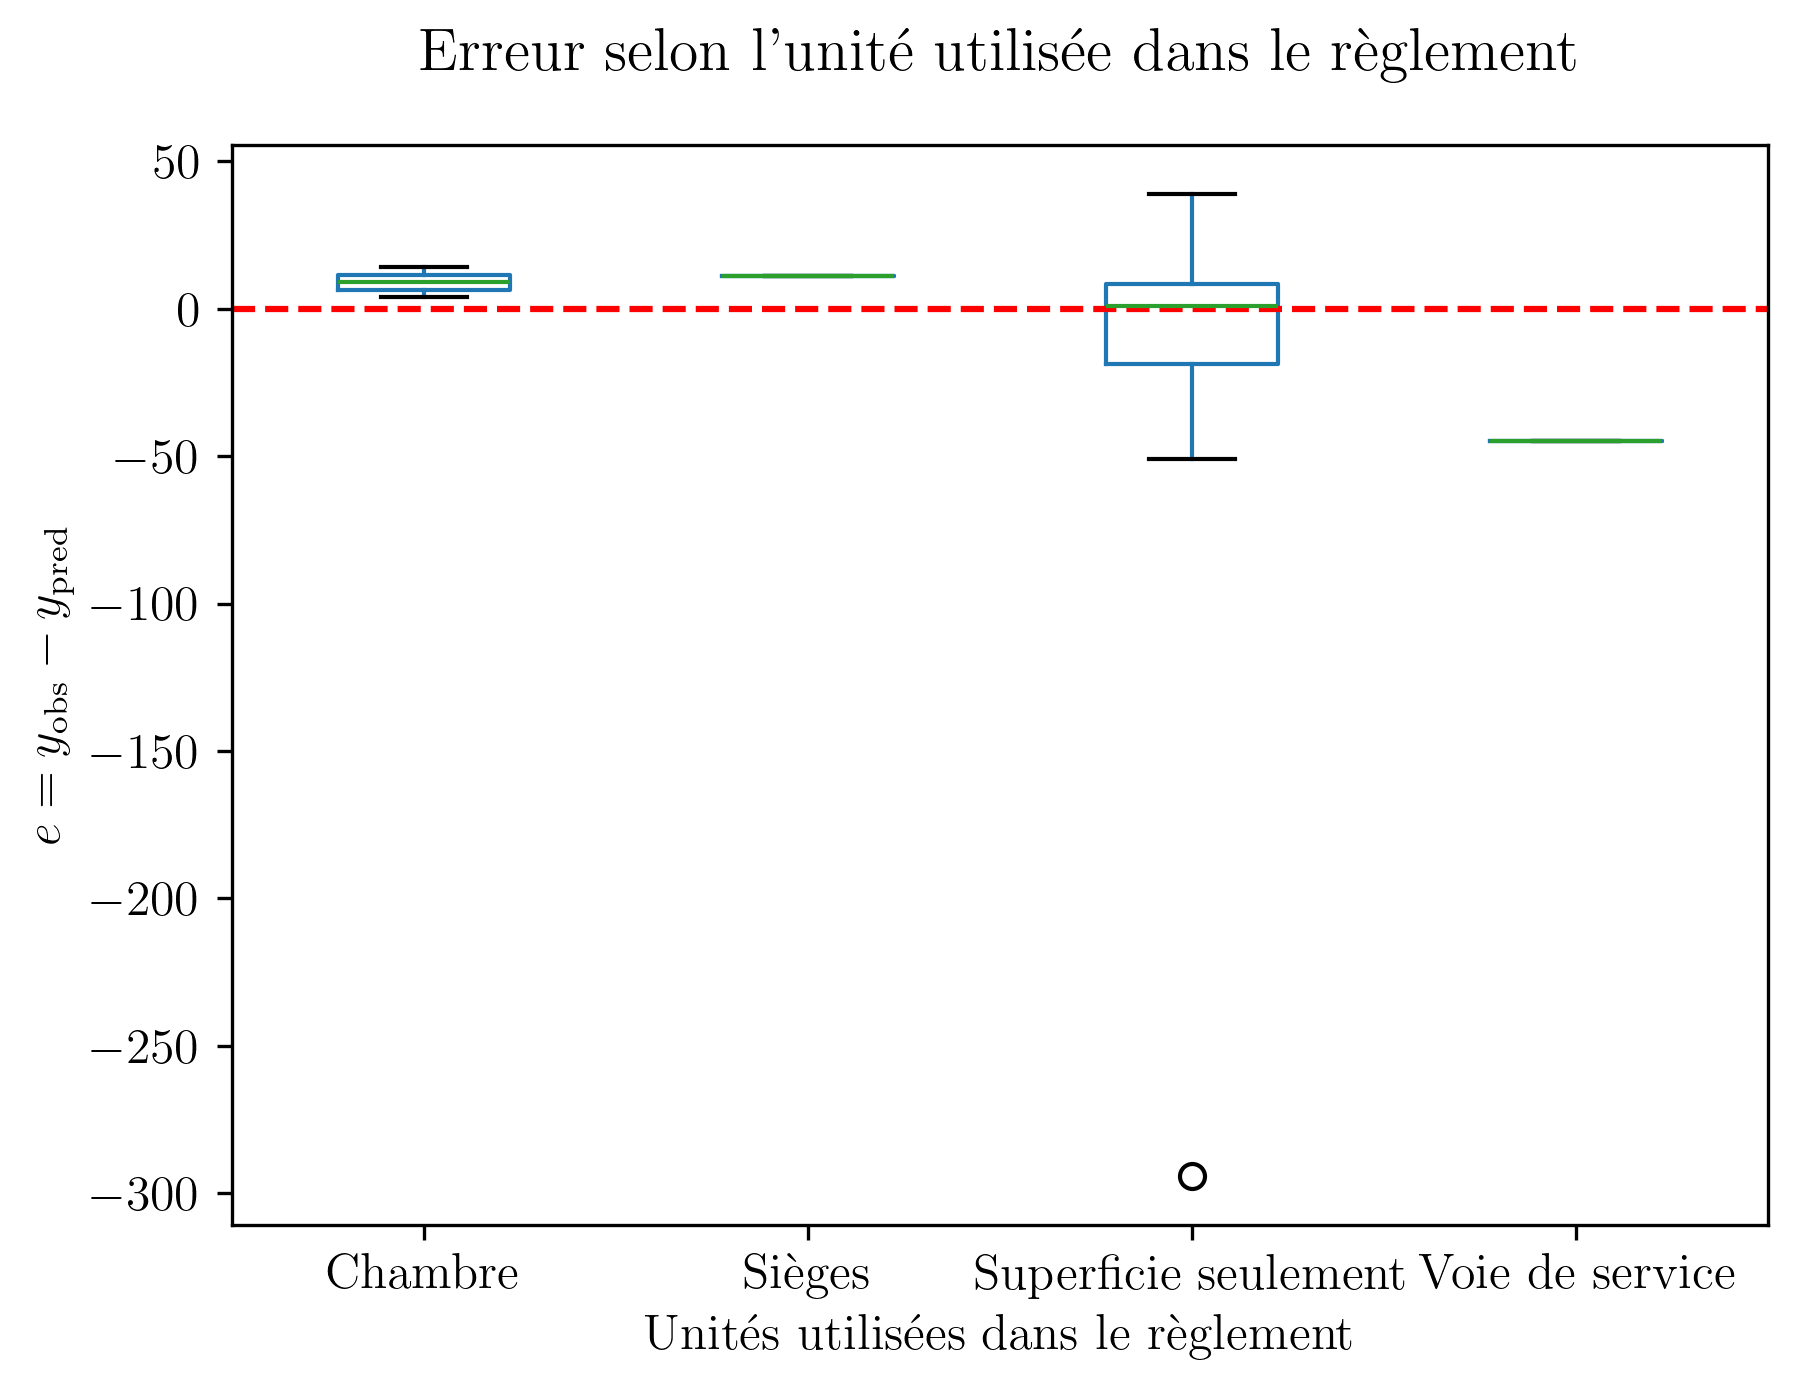
\includegraphics[width=0.8\linewidth]{images/boxplot_error_by_category_40.png}
        \caption{Diagramme à boîte de l'erreur en fonction de l'unité de formulation du règlement pour les propriétés commerciales}
        \label{fig:comm-err-by-unit}
    \end{figure}
    %\begin{figure}
    %    \centering
    %    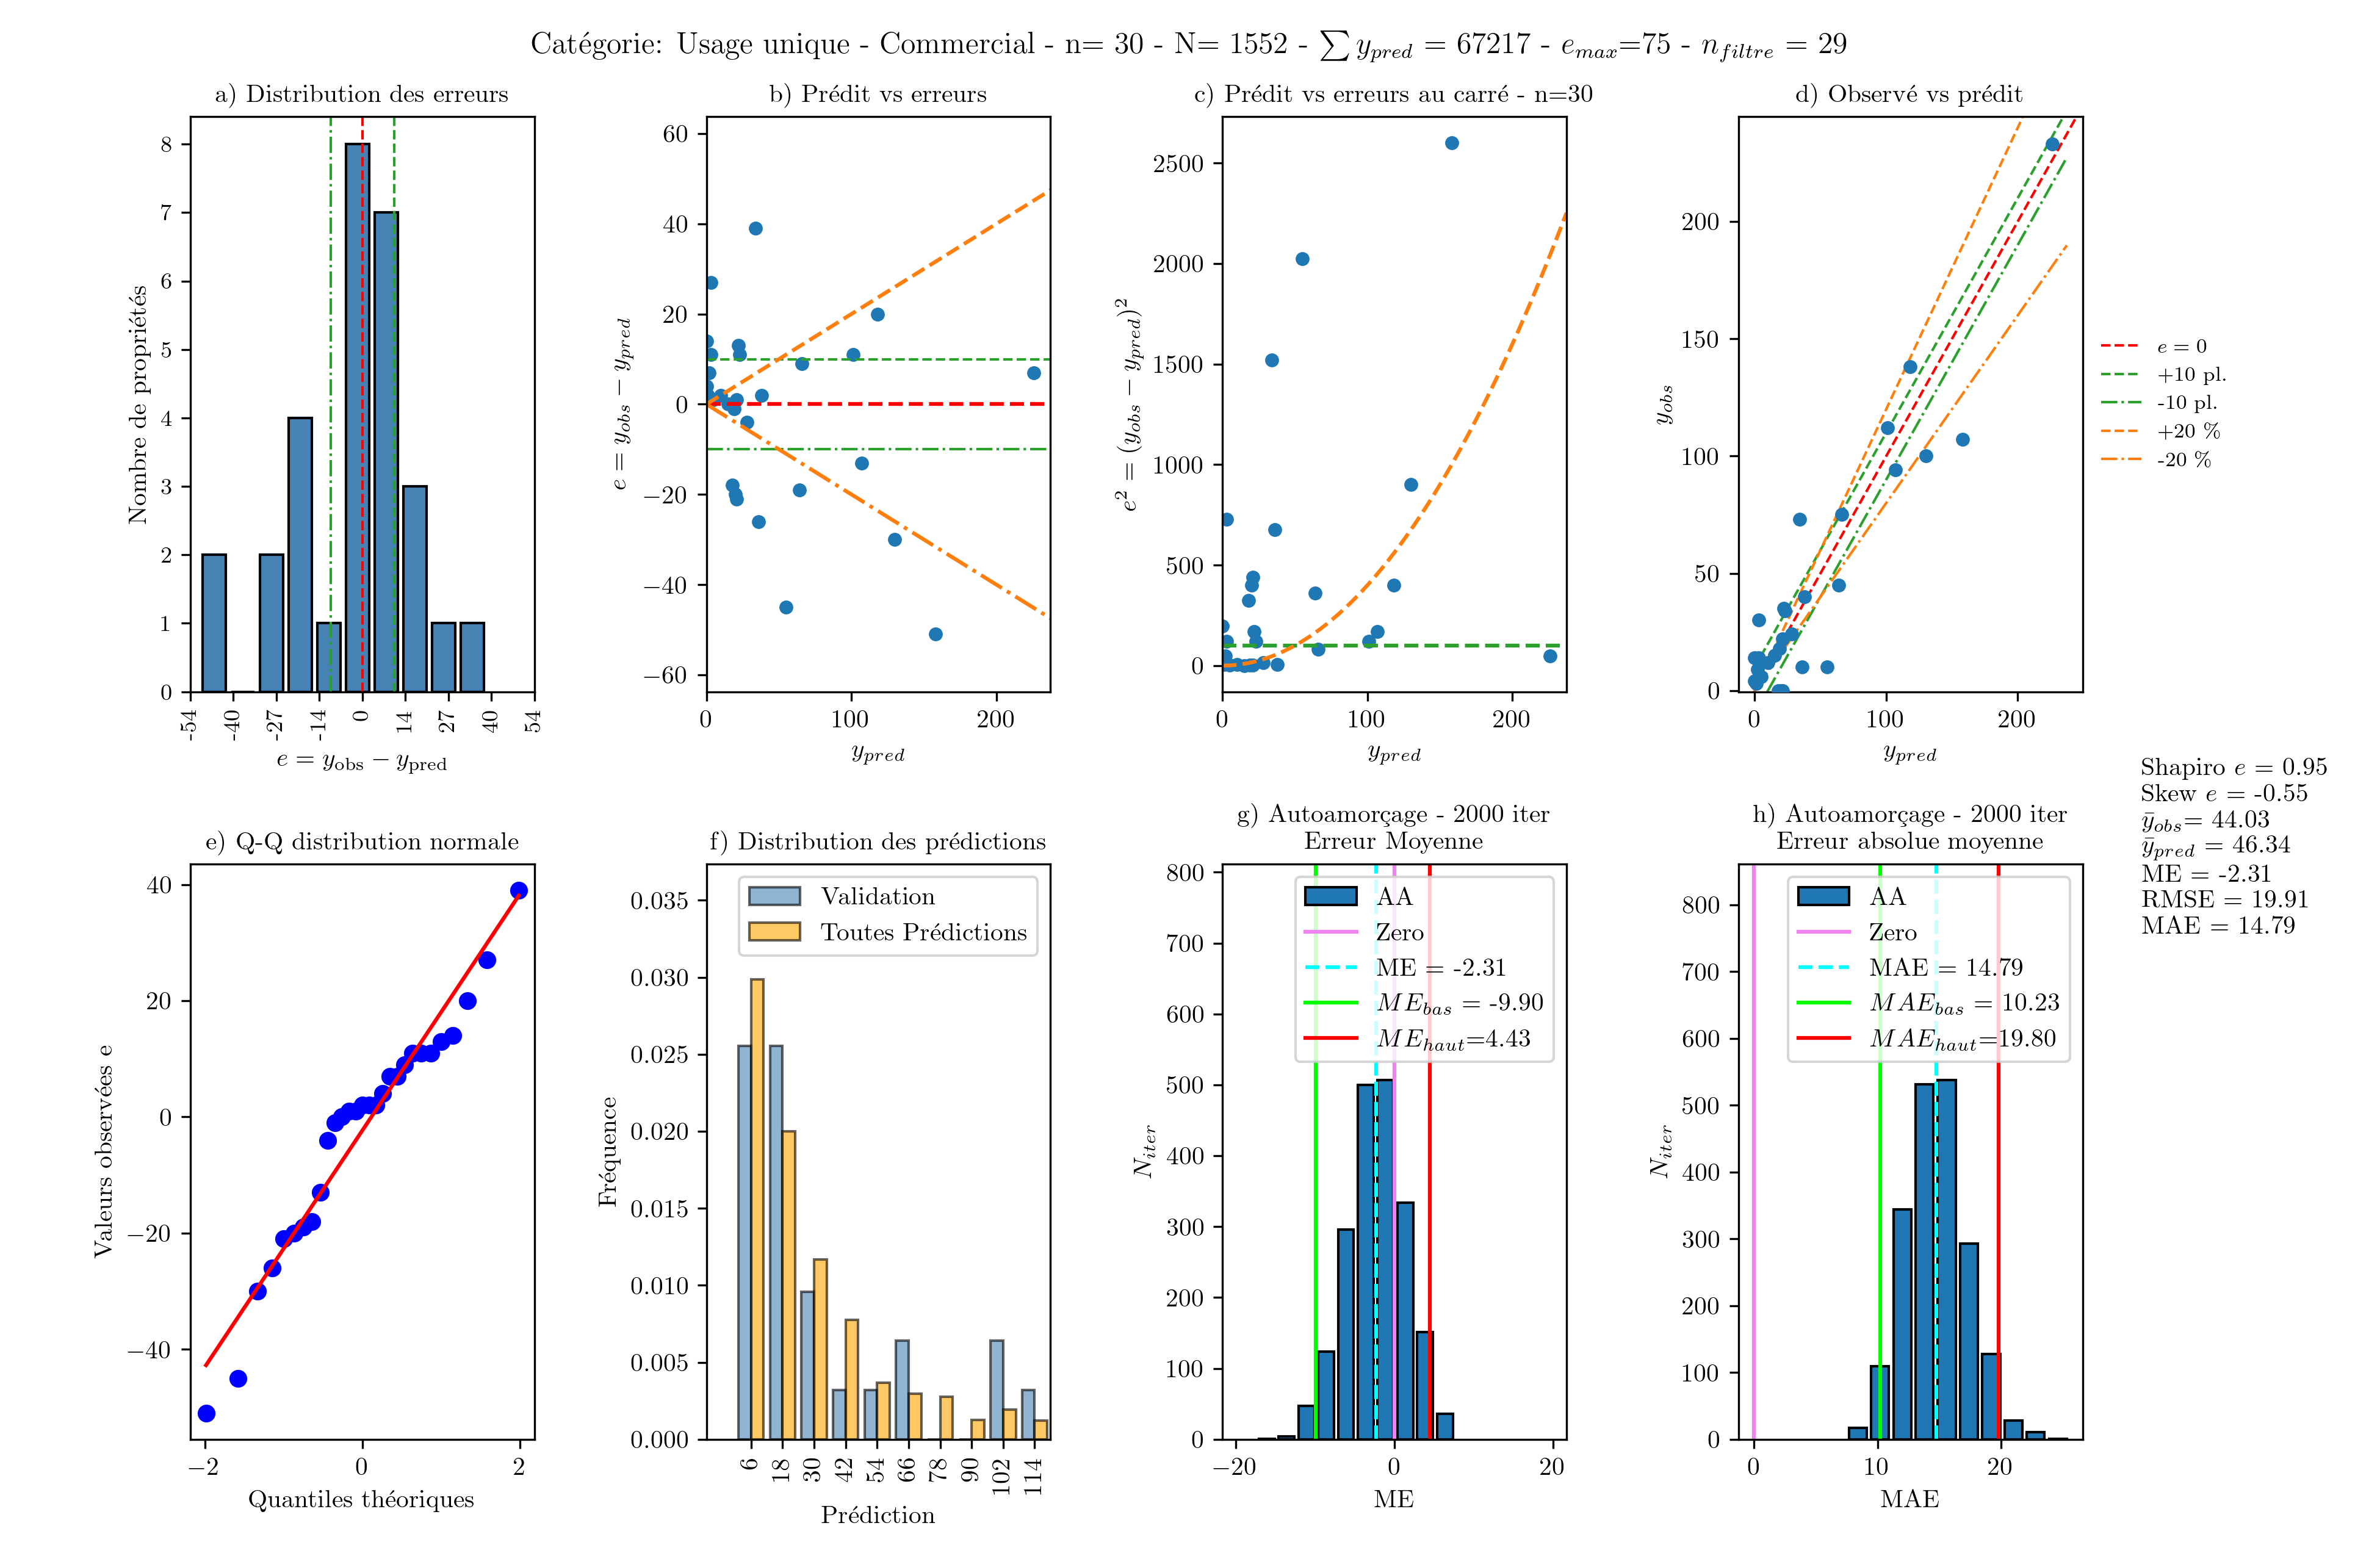
\includegraphics[scale=0.65]{images/int_erreur_40_e_75_se_10_pe_20.png}
    %    \caption{Distribution et intervalles d'erreurs pour les lots commerciaux avec un filtre pour une erreur de plus de 75 places}
    %    \label{fig:intervals-dist-val-comm-e75}
    %\end{figure}
    \begin{figure}[H]
        \centering
        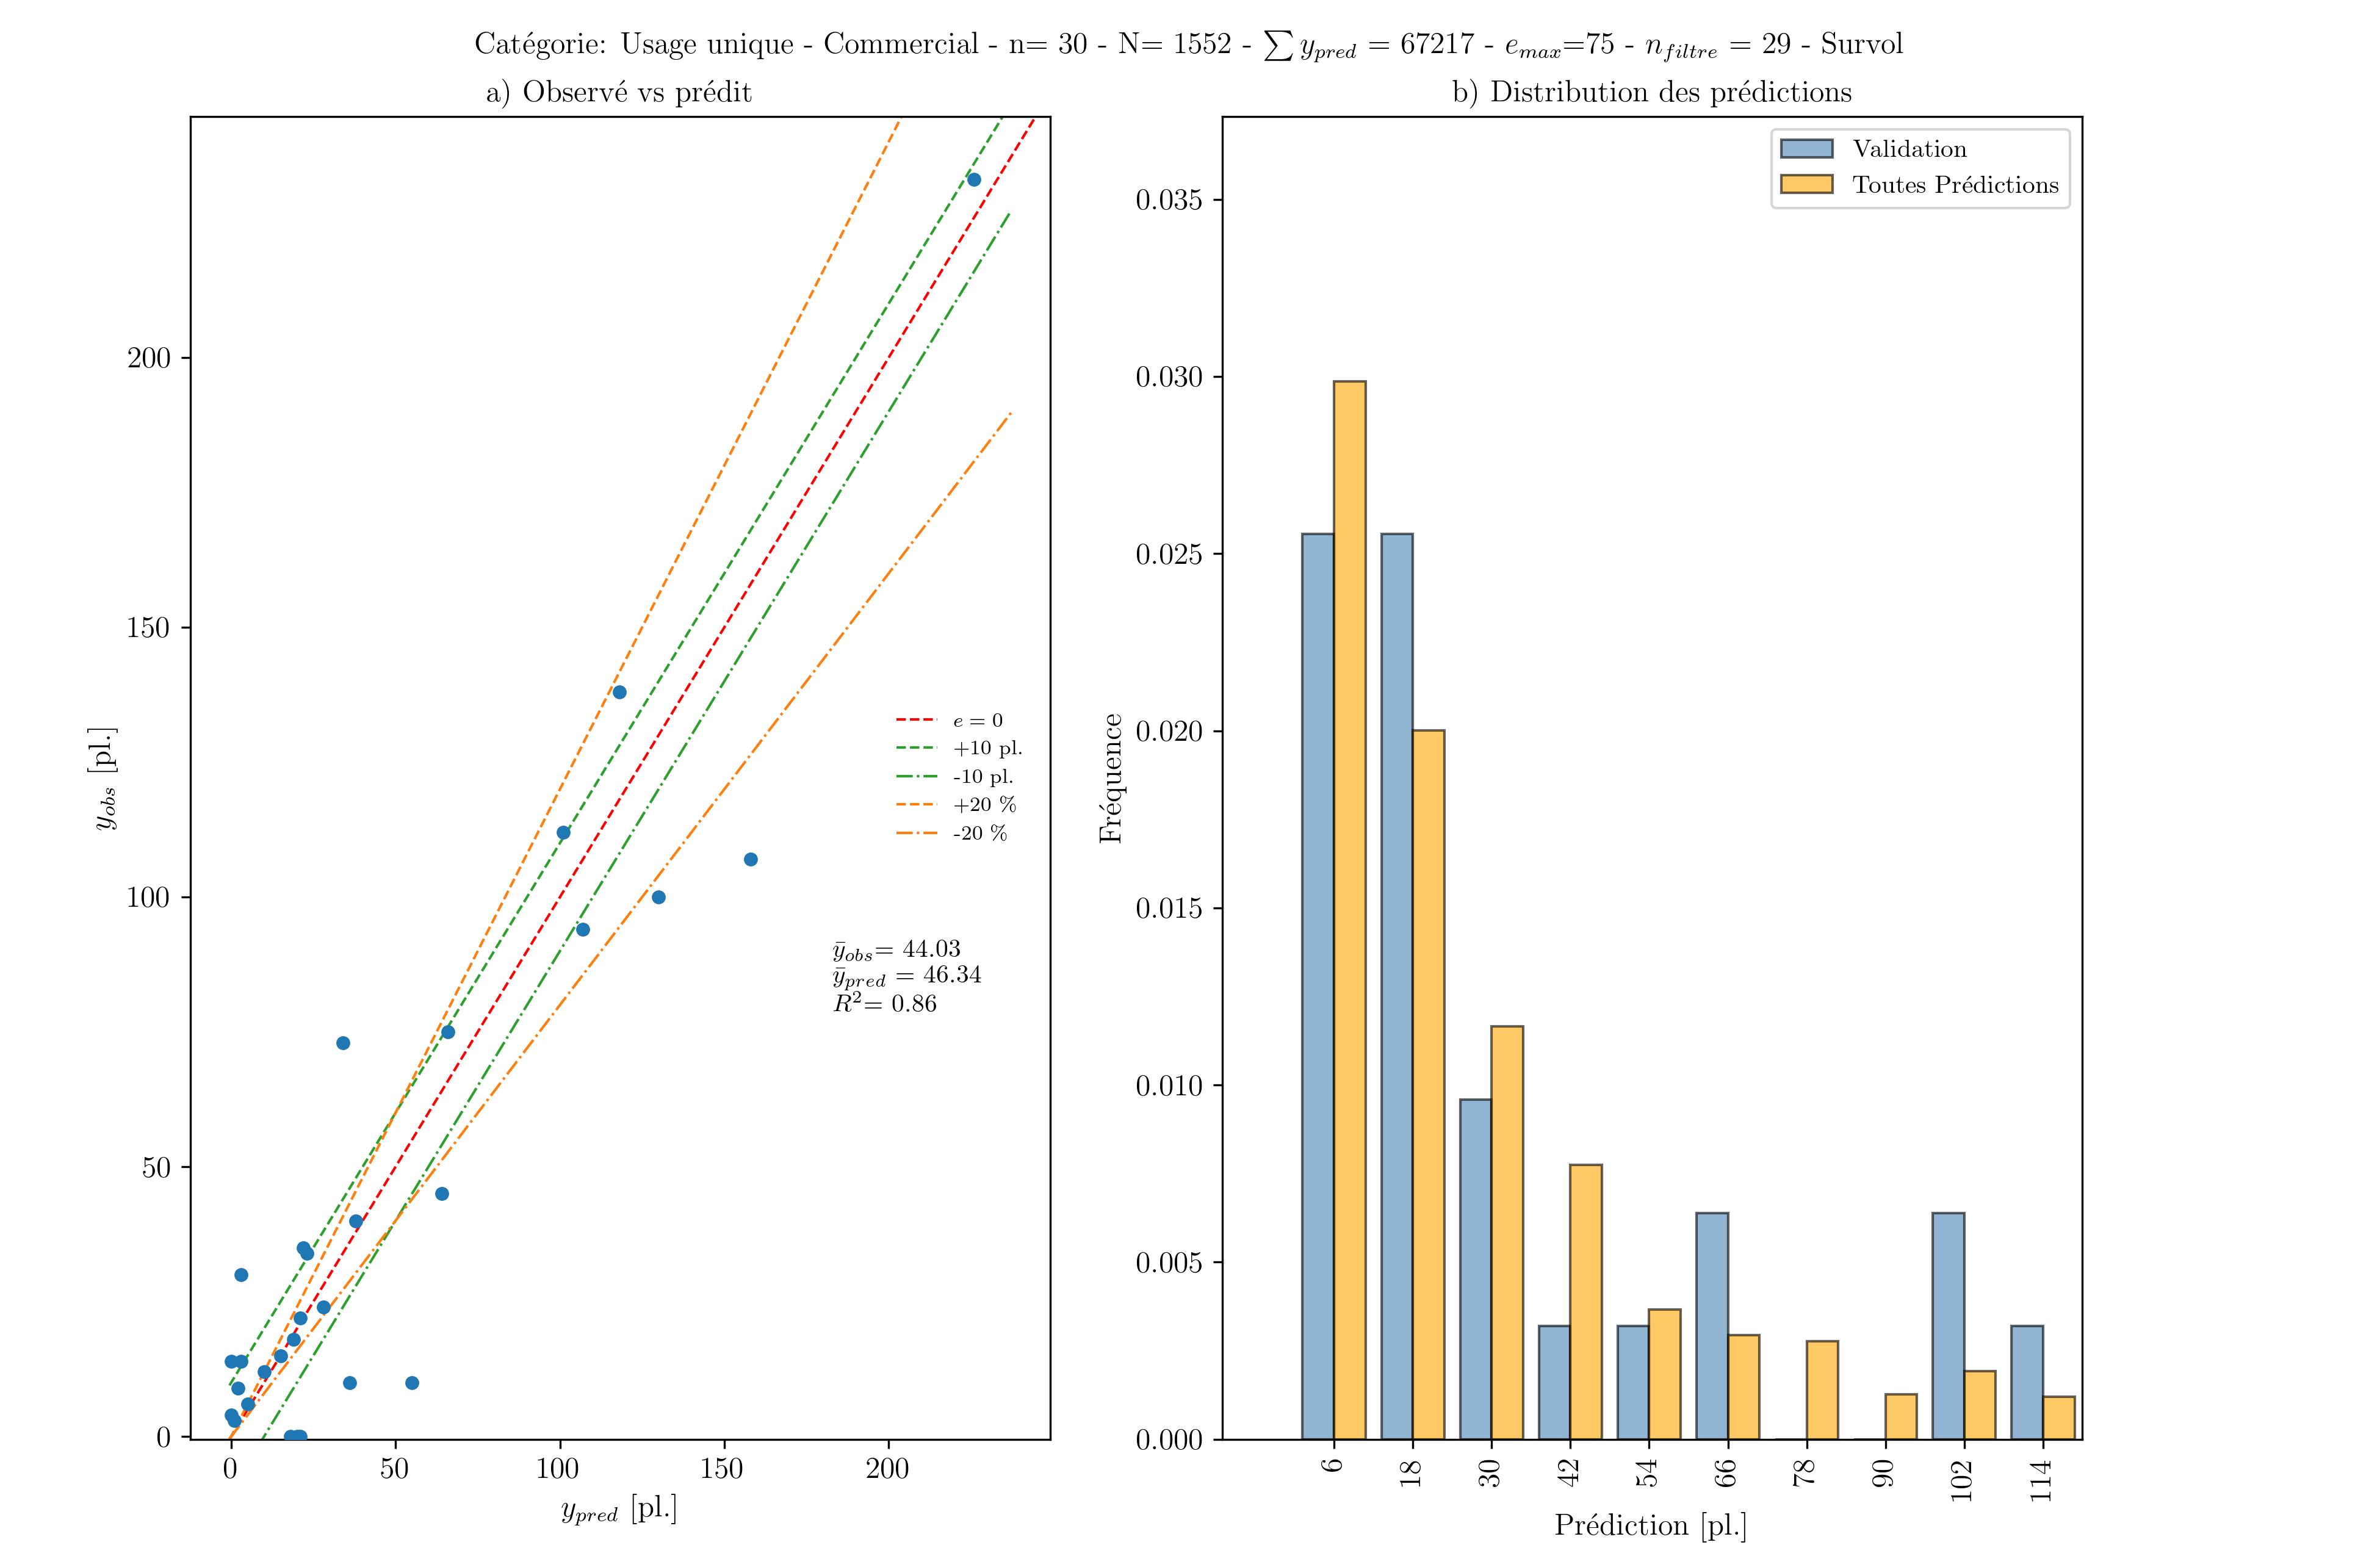
\includegraphics[width=1\linewidth]{images/int_erreur_40_e_75_se_10_pe_20_a.png}
        \caption{Distribution des prédictions pour les lots commerciaux}
        \label{fig:int-dist-pred-comm}
    \end{figure}
    \begin{figure}[H]
        \centering
        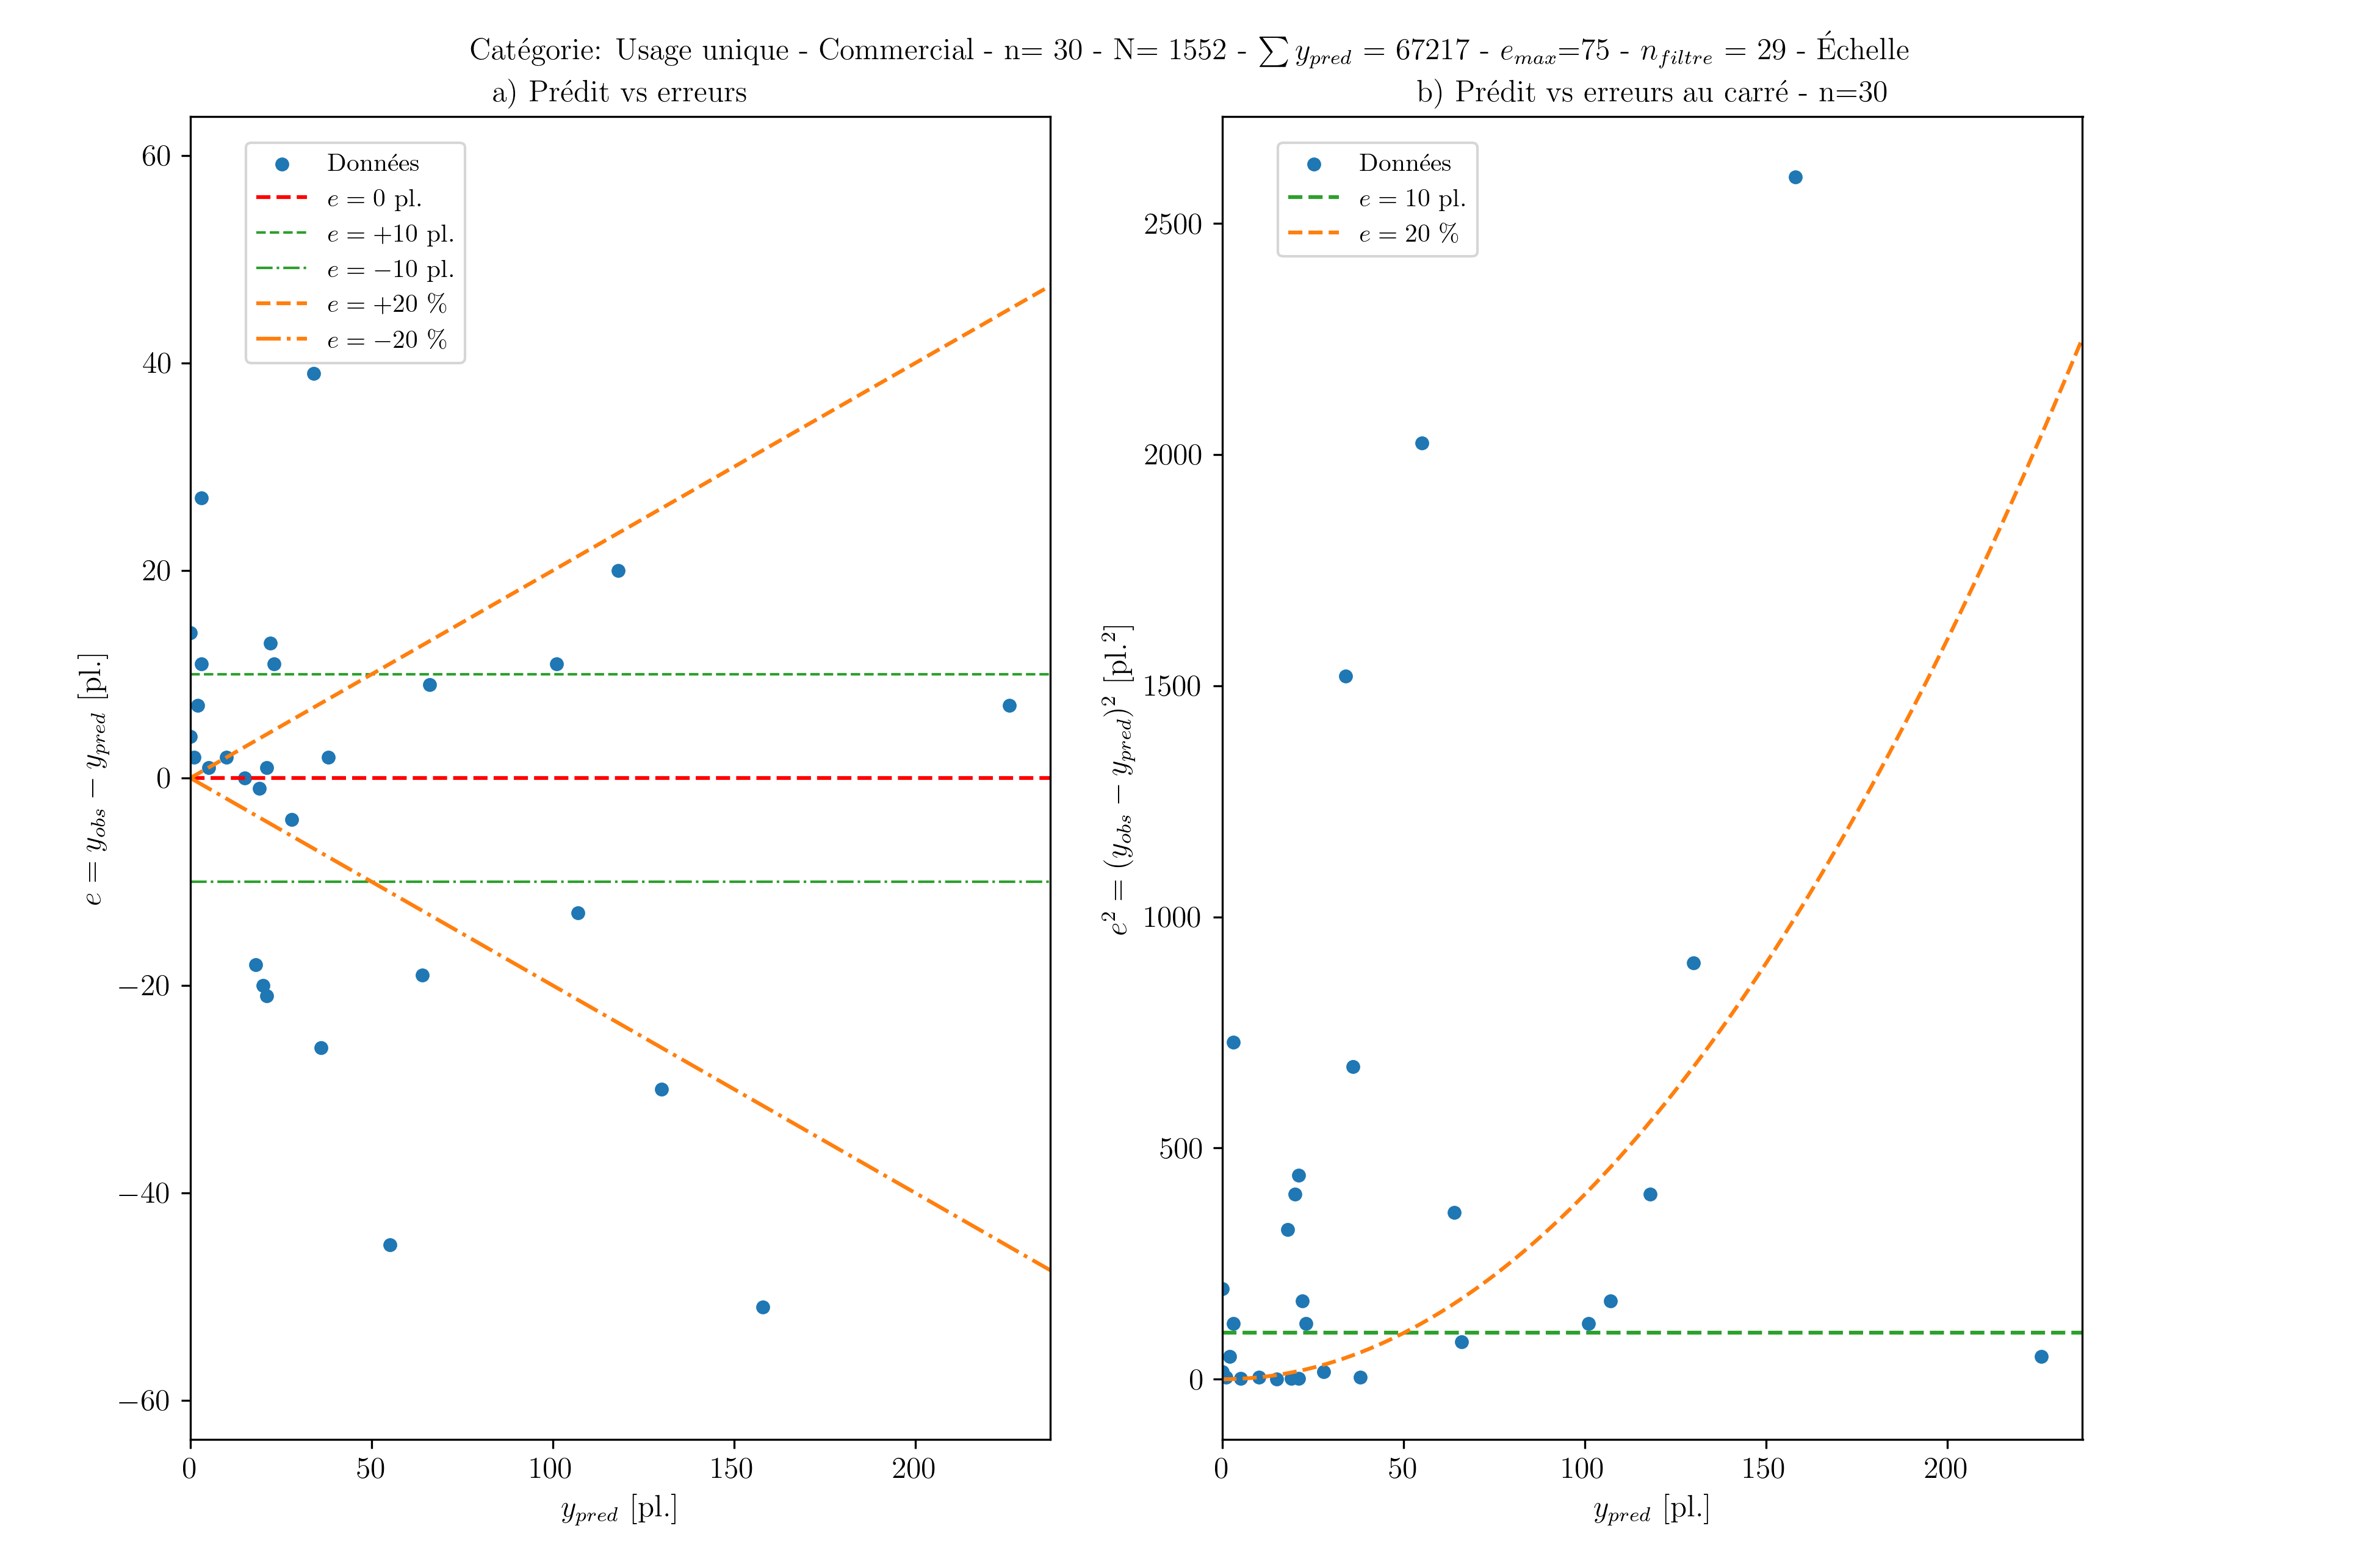
\includegraphics[width=1\linewidth]{images/int_erreur_40_e_75_se_10_pe_20_b.png}
        \caption{Erreur en fonction des prédictions pour les lots commerciaux}
        \label{fig:err-err-quad-pred-comm}
    \end{figure}
    \begin{figure}[H]
        \centering
        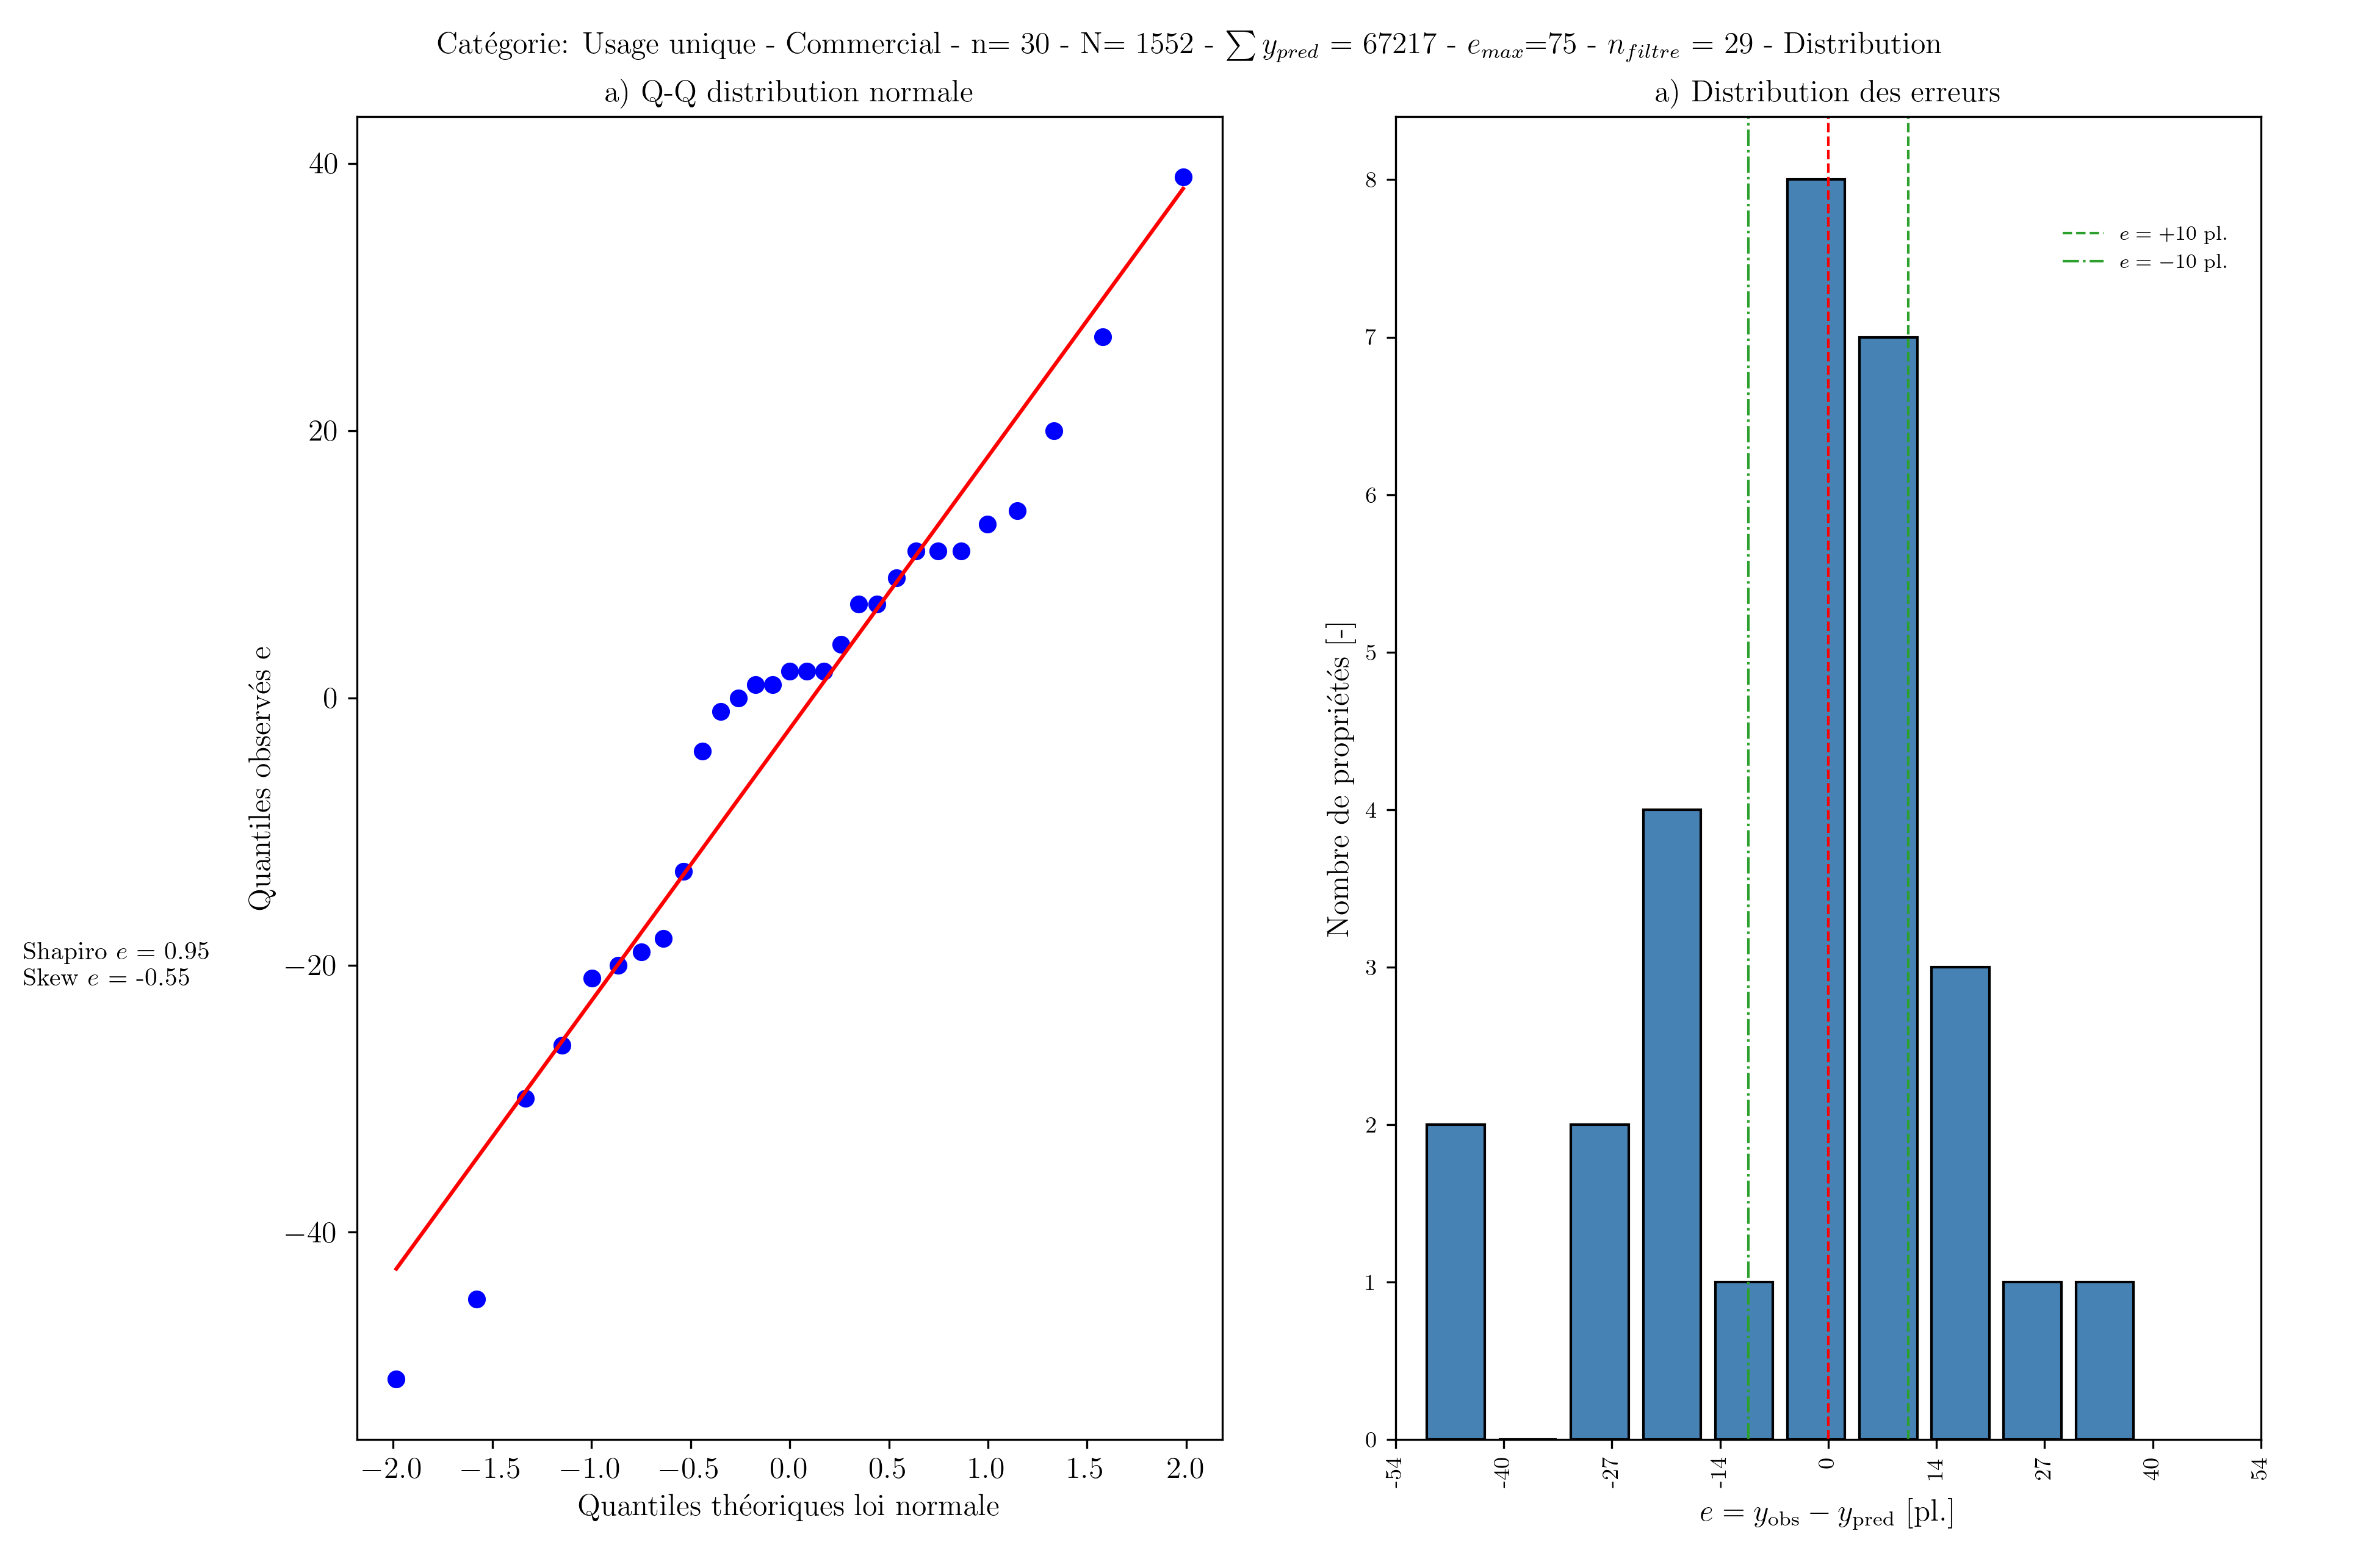
\includegraphics[width=1\linewidth]{images/int_erreur_40_e_75_se_10_pe_20_c.png}
        \caption{Distribution et normalité des erreurs pour les lots commerciaux}
        \label{fig:dist-erreur-norm-comm}
    \end{figure}
    \begin{figure}[H]
        \centering
        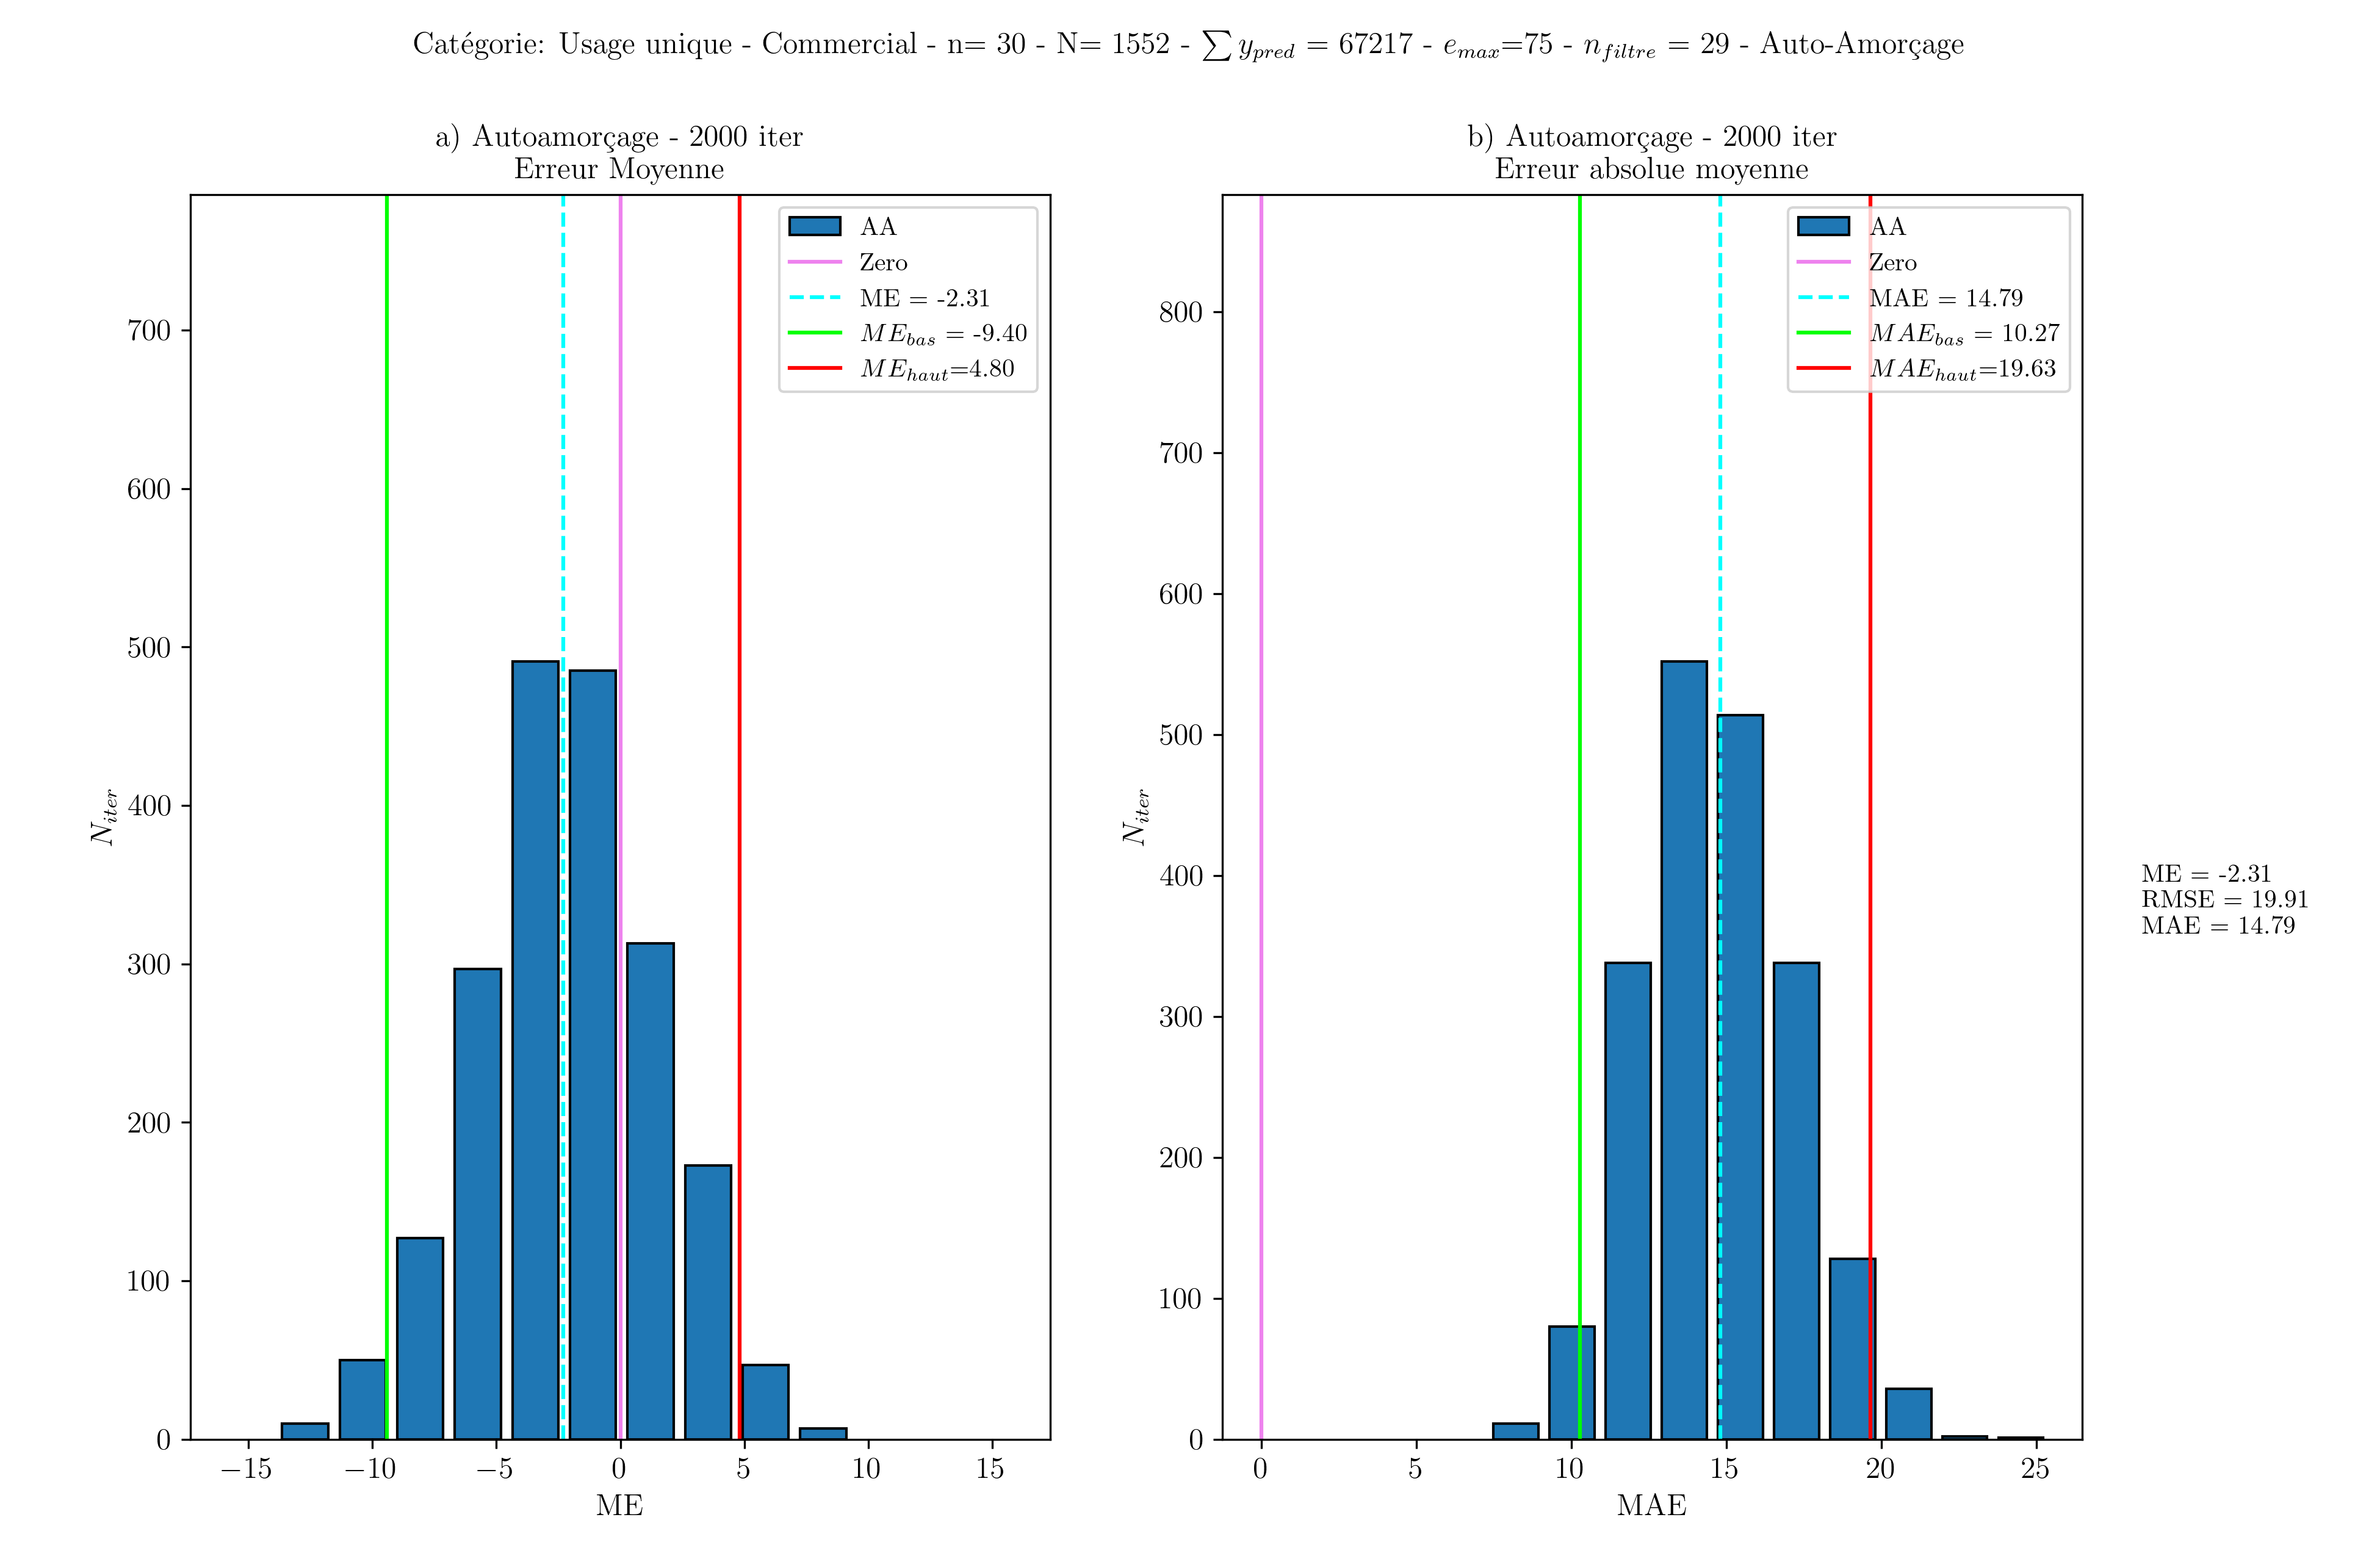
\includegraphics[width=1\linewidth]{images/int_erreur_40_e_75_se_10_pe_20_d.png}
        \caption{Distribution des métriques d'erreur après auto-amorçage pour les lots commerciaux}
        \label{fig:auto-amor-comm}
    \end{figure}
    %\begin{figure}[H]
    %    \centering
    %    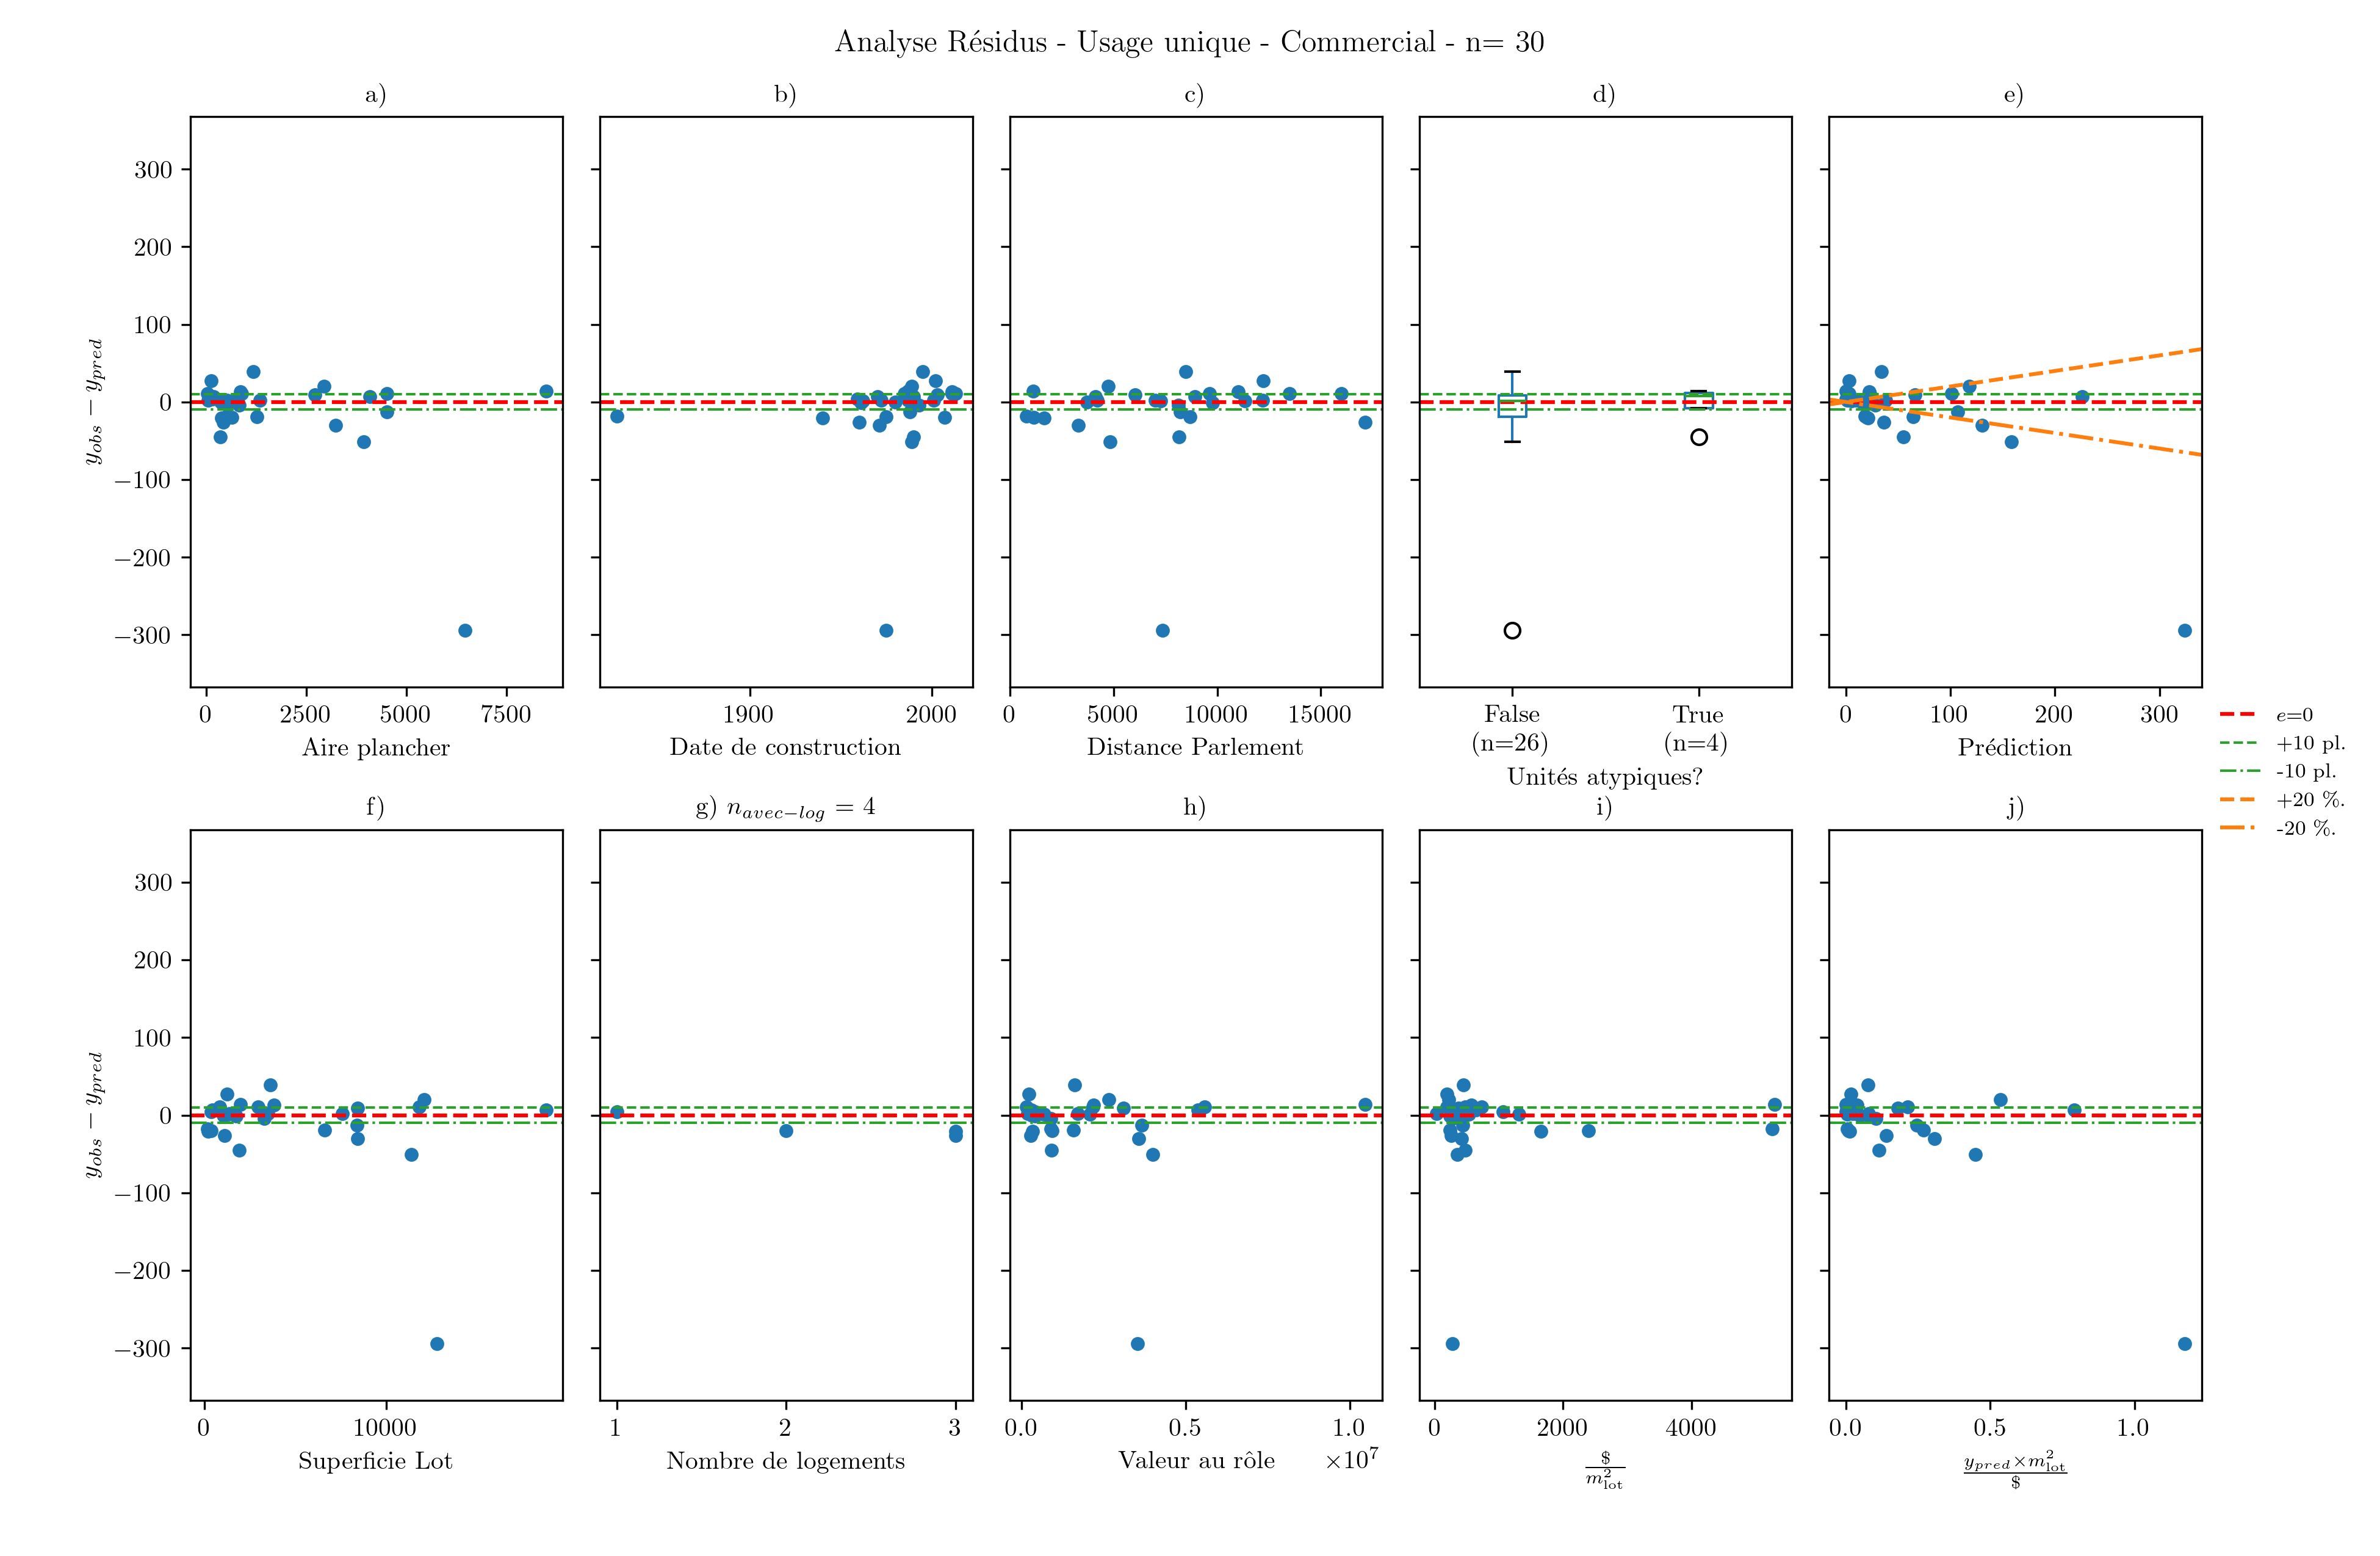
\includegraphics[scale=0.65]{images/ana_res_40_se_10_pe_20.png}
    %    \caption{Analyse des résidus des propriétés commerciales sans filtre}
    %    \label{fig:ana-residu-comm}
    %\end{figure}
    \begin{figure}[H]
        \centering
        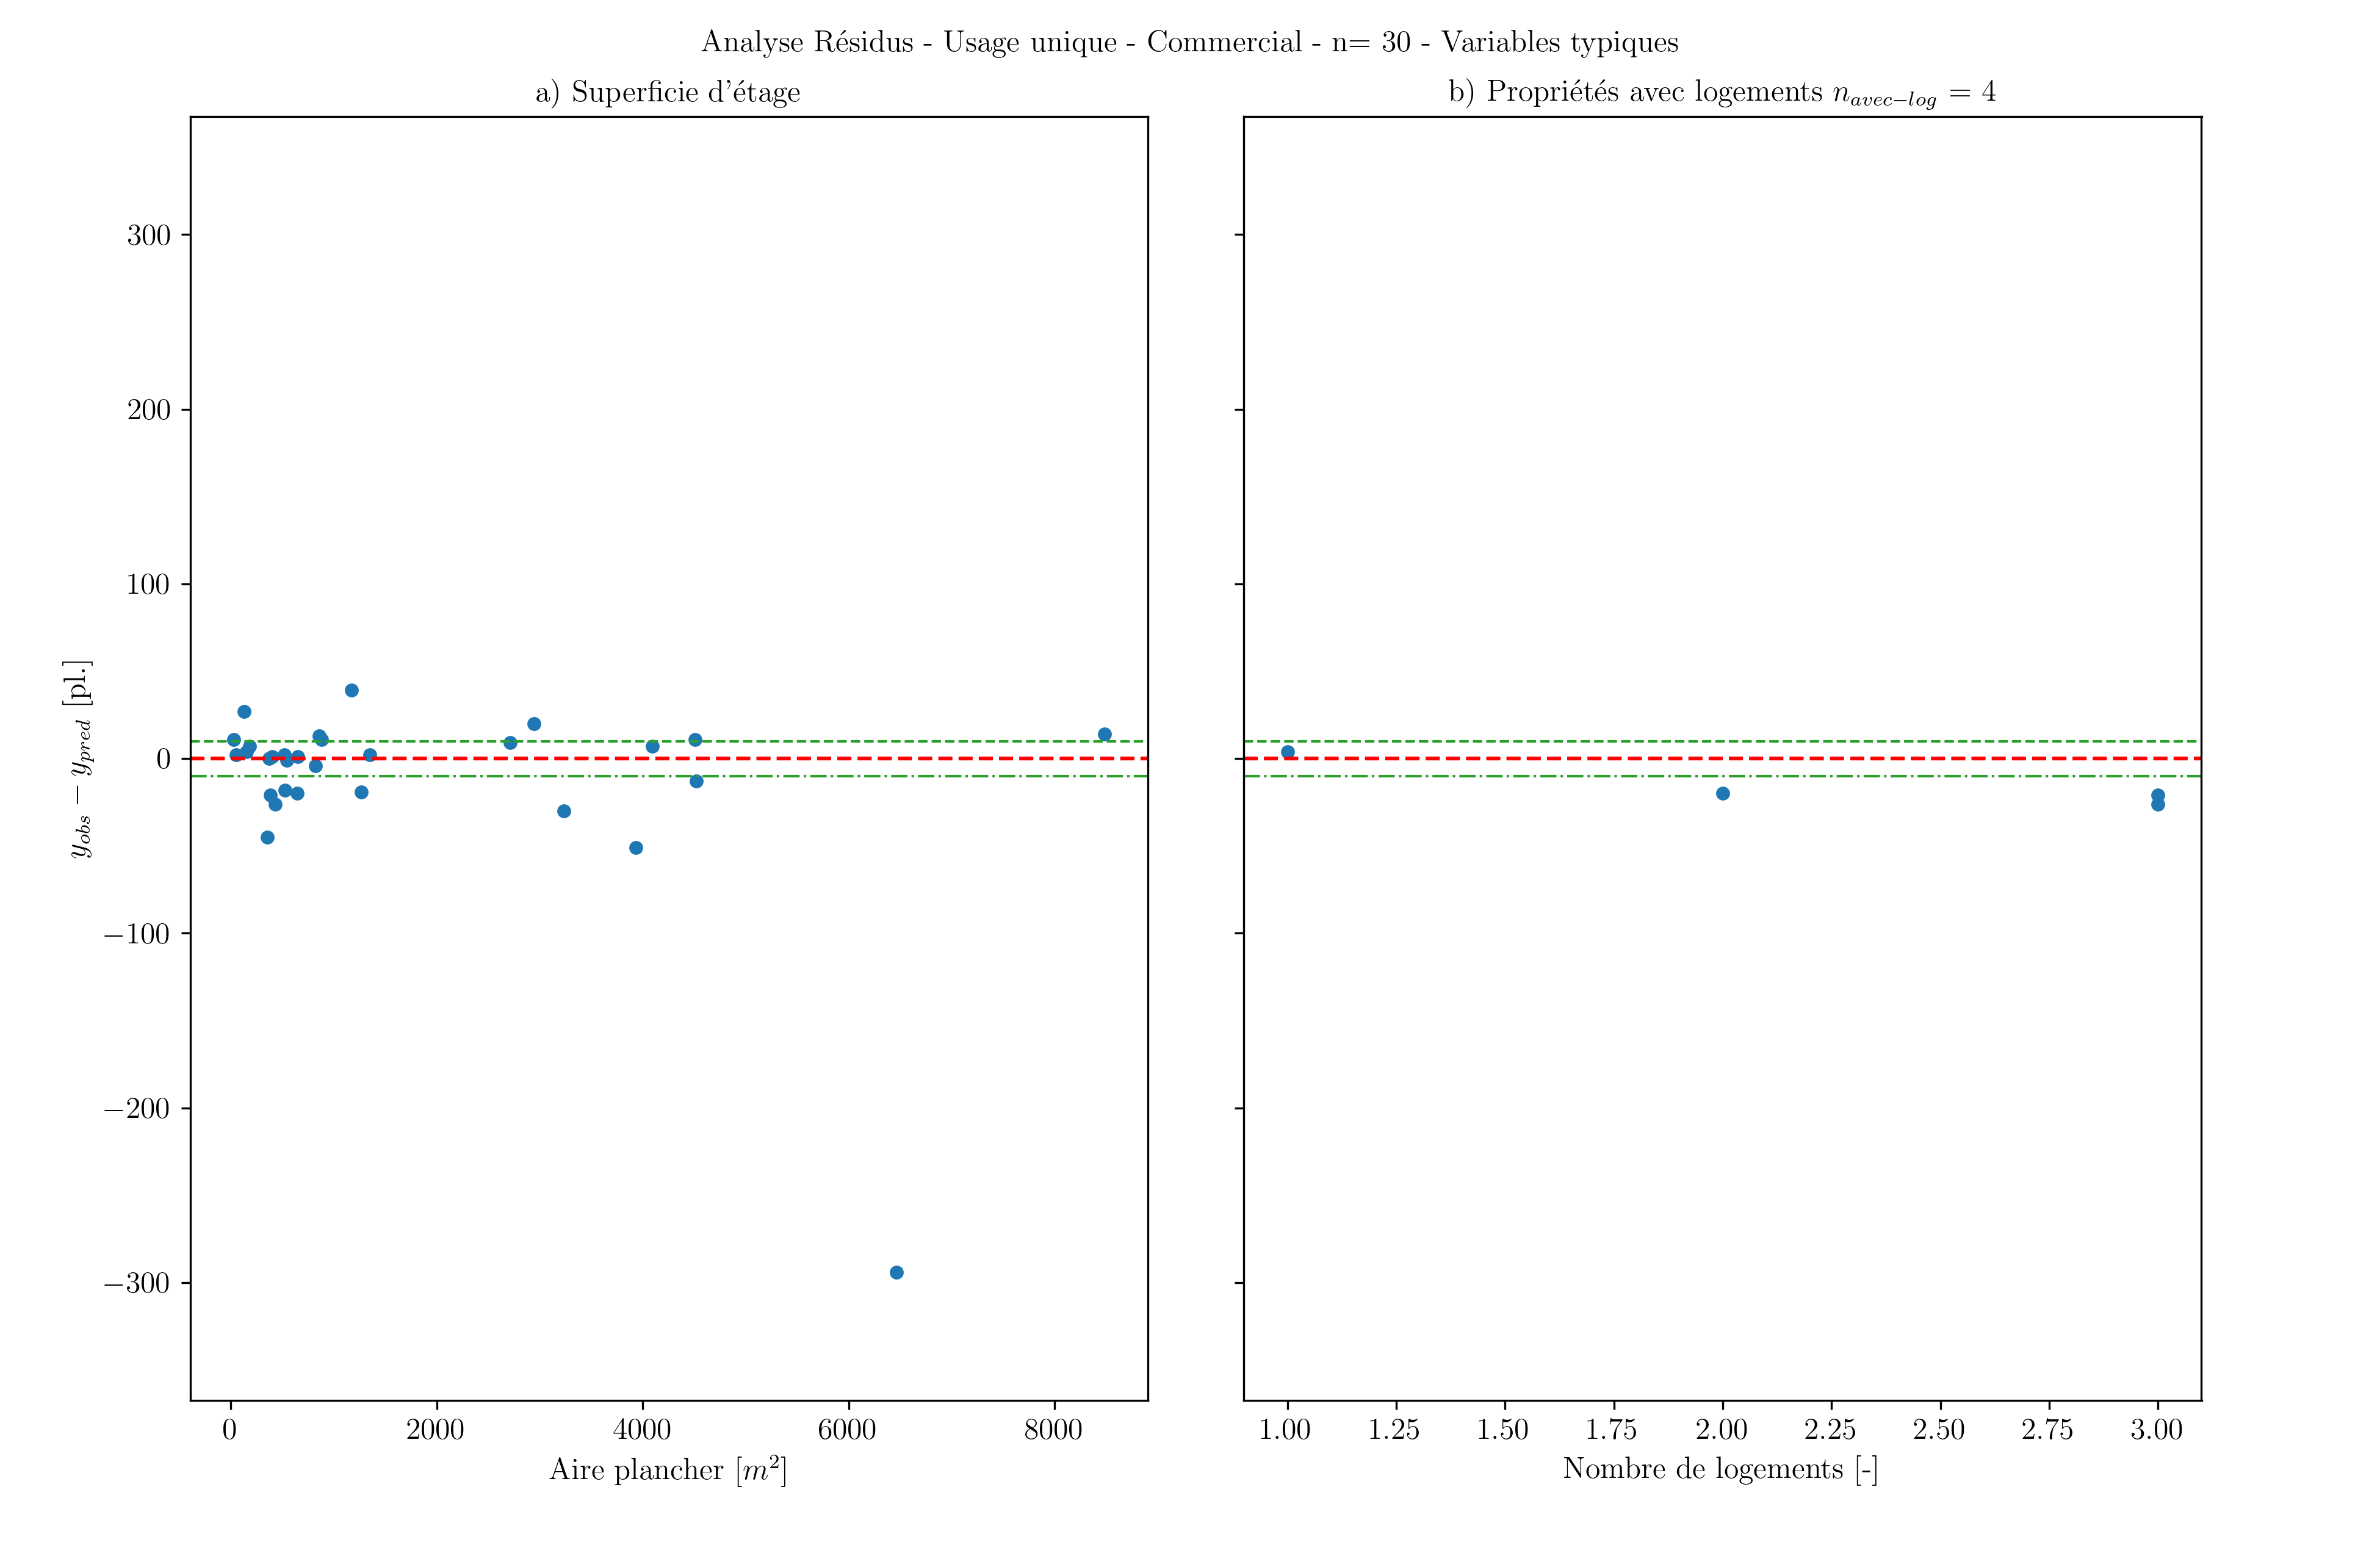
\includegraphics[width=1\linewidth]{images/ana_res_40_se_10_pe_20_a.png}
        \caption{Analyse des résidus en fonction des propriétés de construction pour les lots commerciaux}
        \label{fig:ana-res-prop-phys-comm}
    \end{figure}
    \begin{figure}[H]
        \centering
        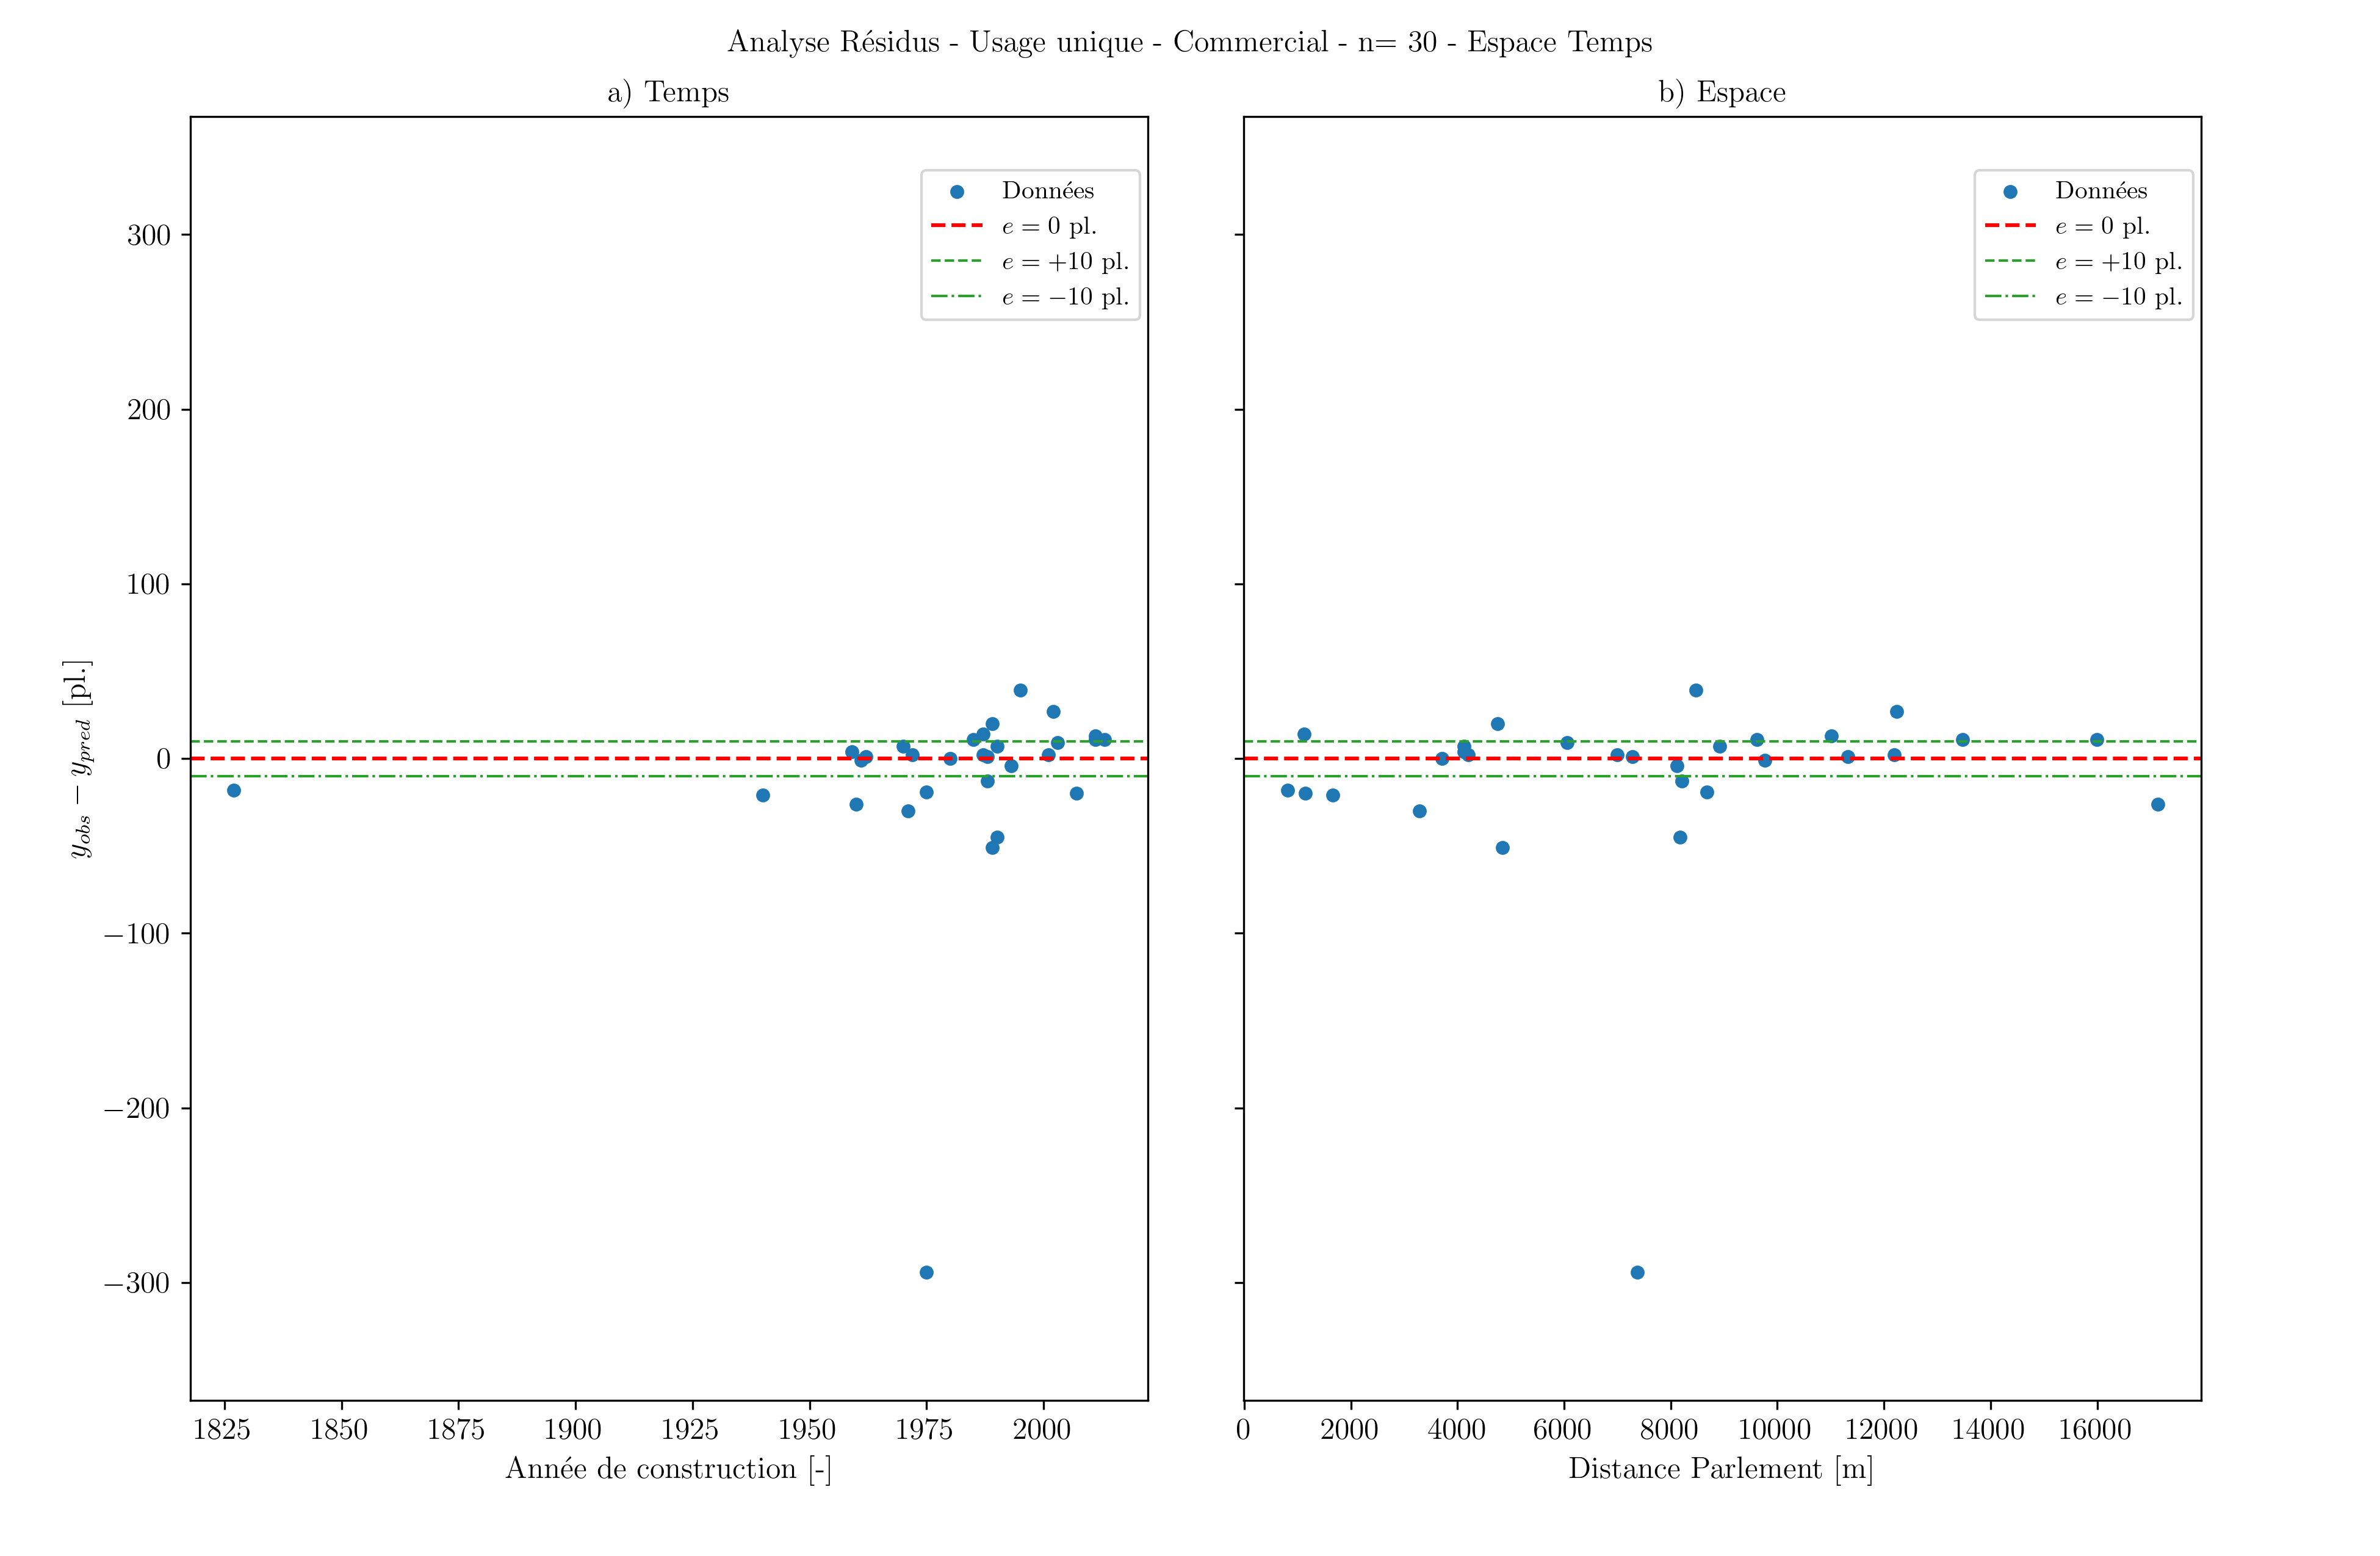
\includegraphics[width=1\linewidth]{images/ana_res_40_se_10_pe_20_b.png}
        \caption{Analyse des résidus en fonction de l'espace et de l'époque de construction pour les lots commerciaux}
        \label{fig:ana-res-esp-temps-comm}
    \end{figure}
    \begin{figure}[H]
        \centering
        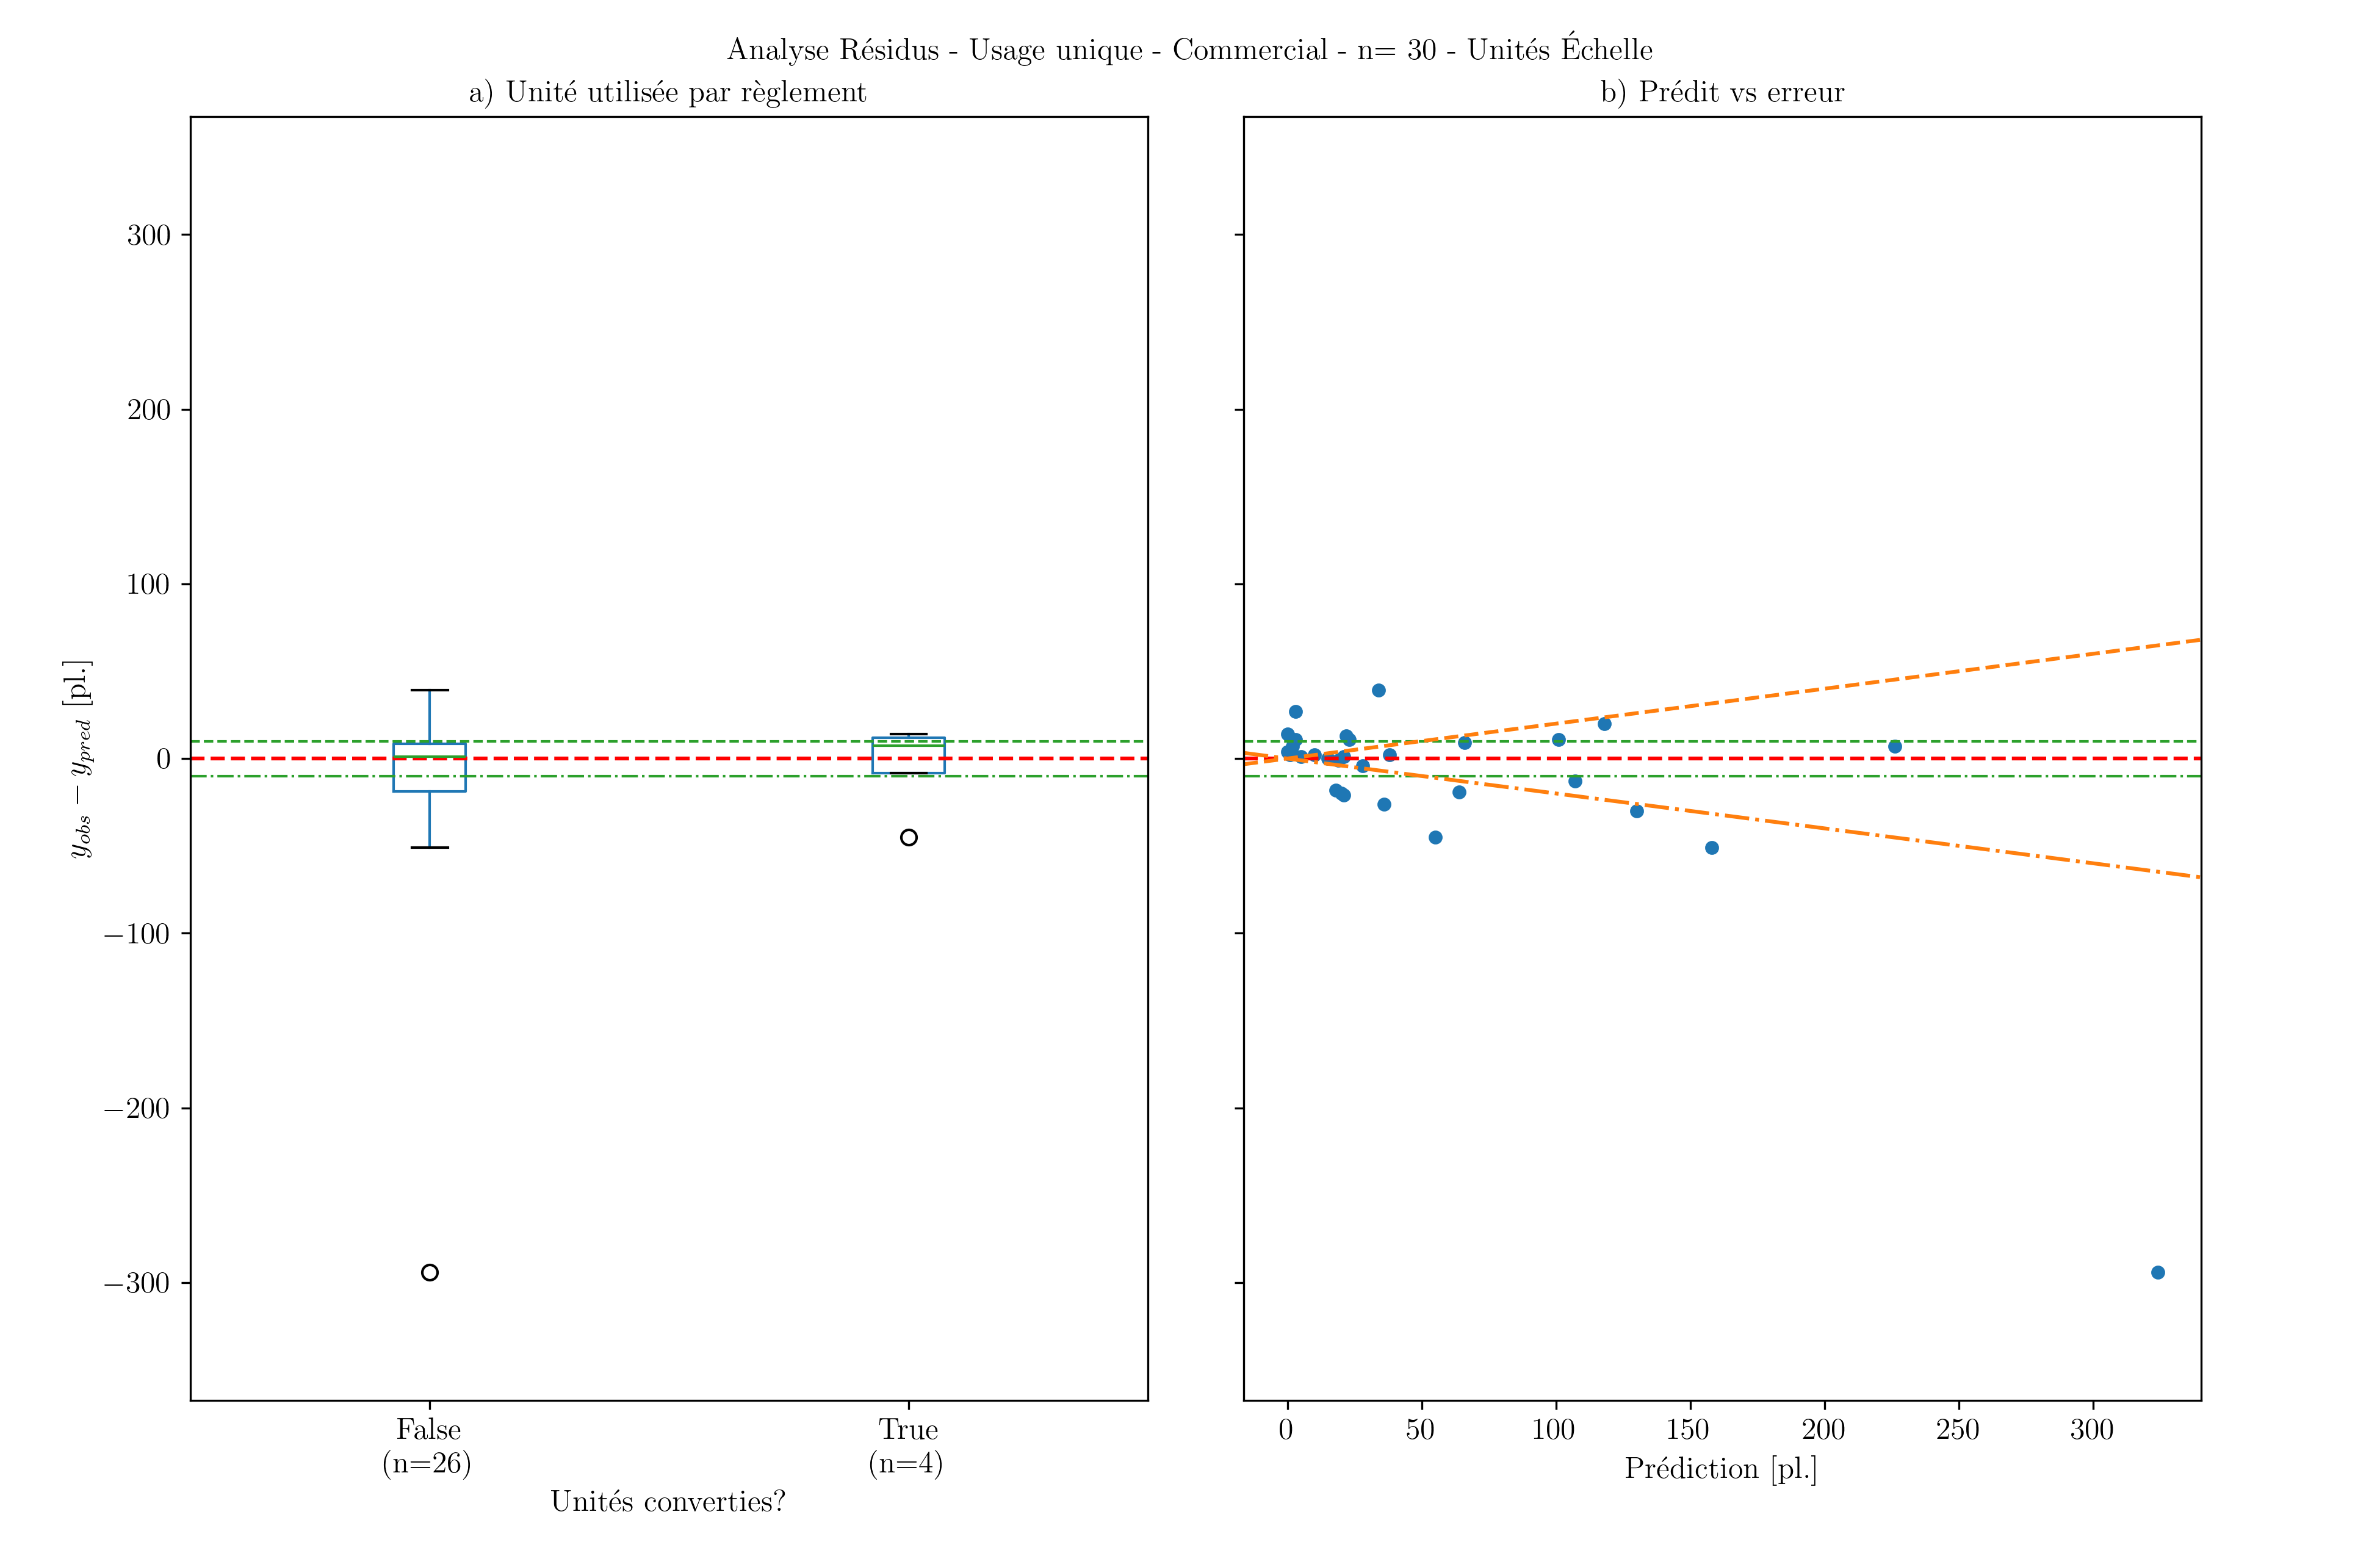
\includegraphics[width=1\linewidth]{images/ana_res_40_se_10_pe_20_c.png}
        \caption{Analyse des résidus en fonction de la prédiction et des unités de formulation pour les lots commerciaux}
        \label{fig:ana-res-unit-pred-comm}
    \end{figure}
    \begin{figure}[H]
        \centering
        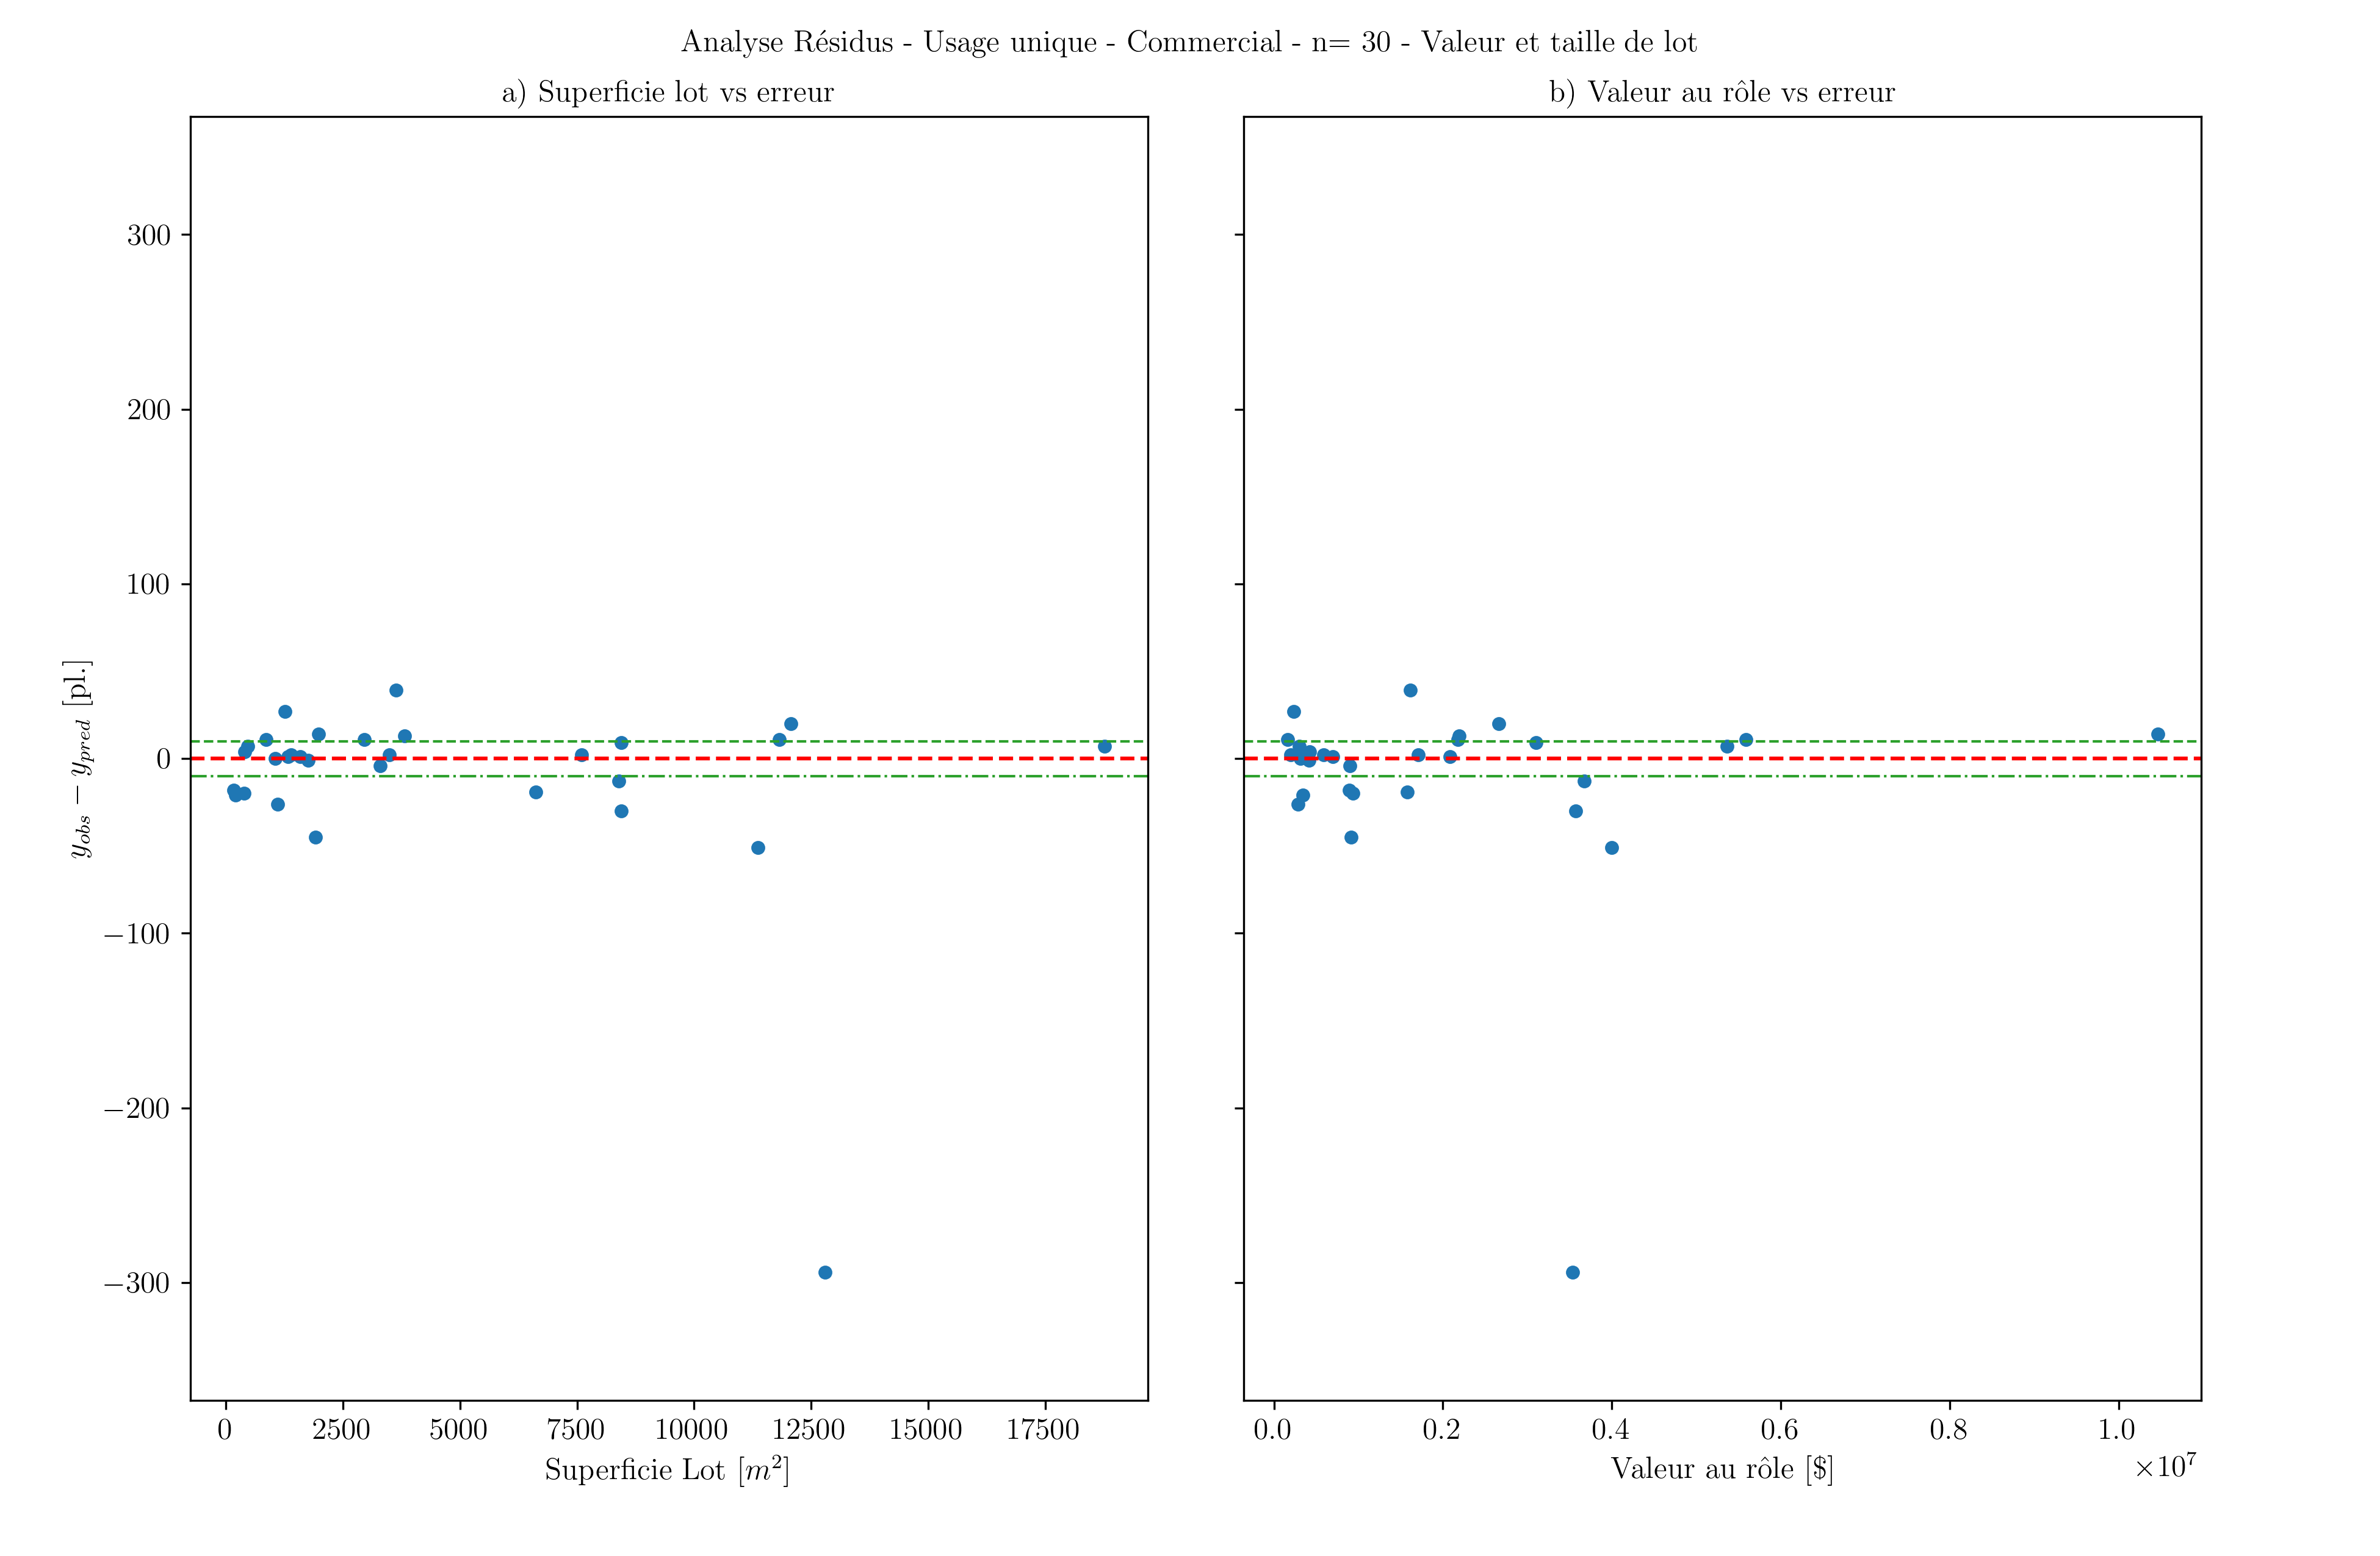
\includegraphics[width=1\linewidth]{images/ana_res_40_se_10_pe_20_d.png}
        \caption{Analyse des résidus en fonction de la superficie du lot et de la valeur pour les lots commerciaux}
        \label{fig:ana-res-sup-val-comm}
    \end{figure}
    \begin{figure}[H]
        \centering
        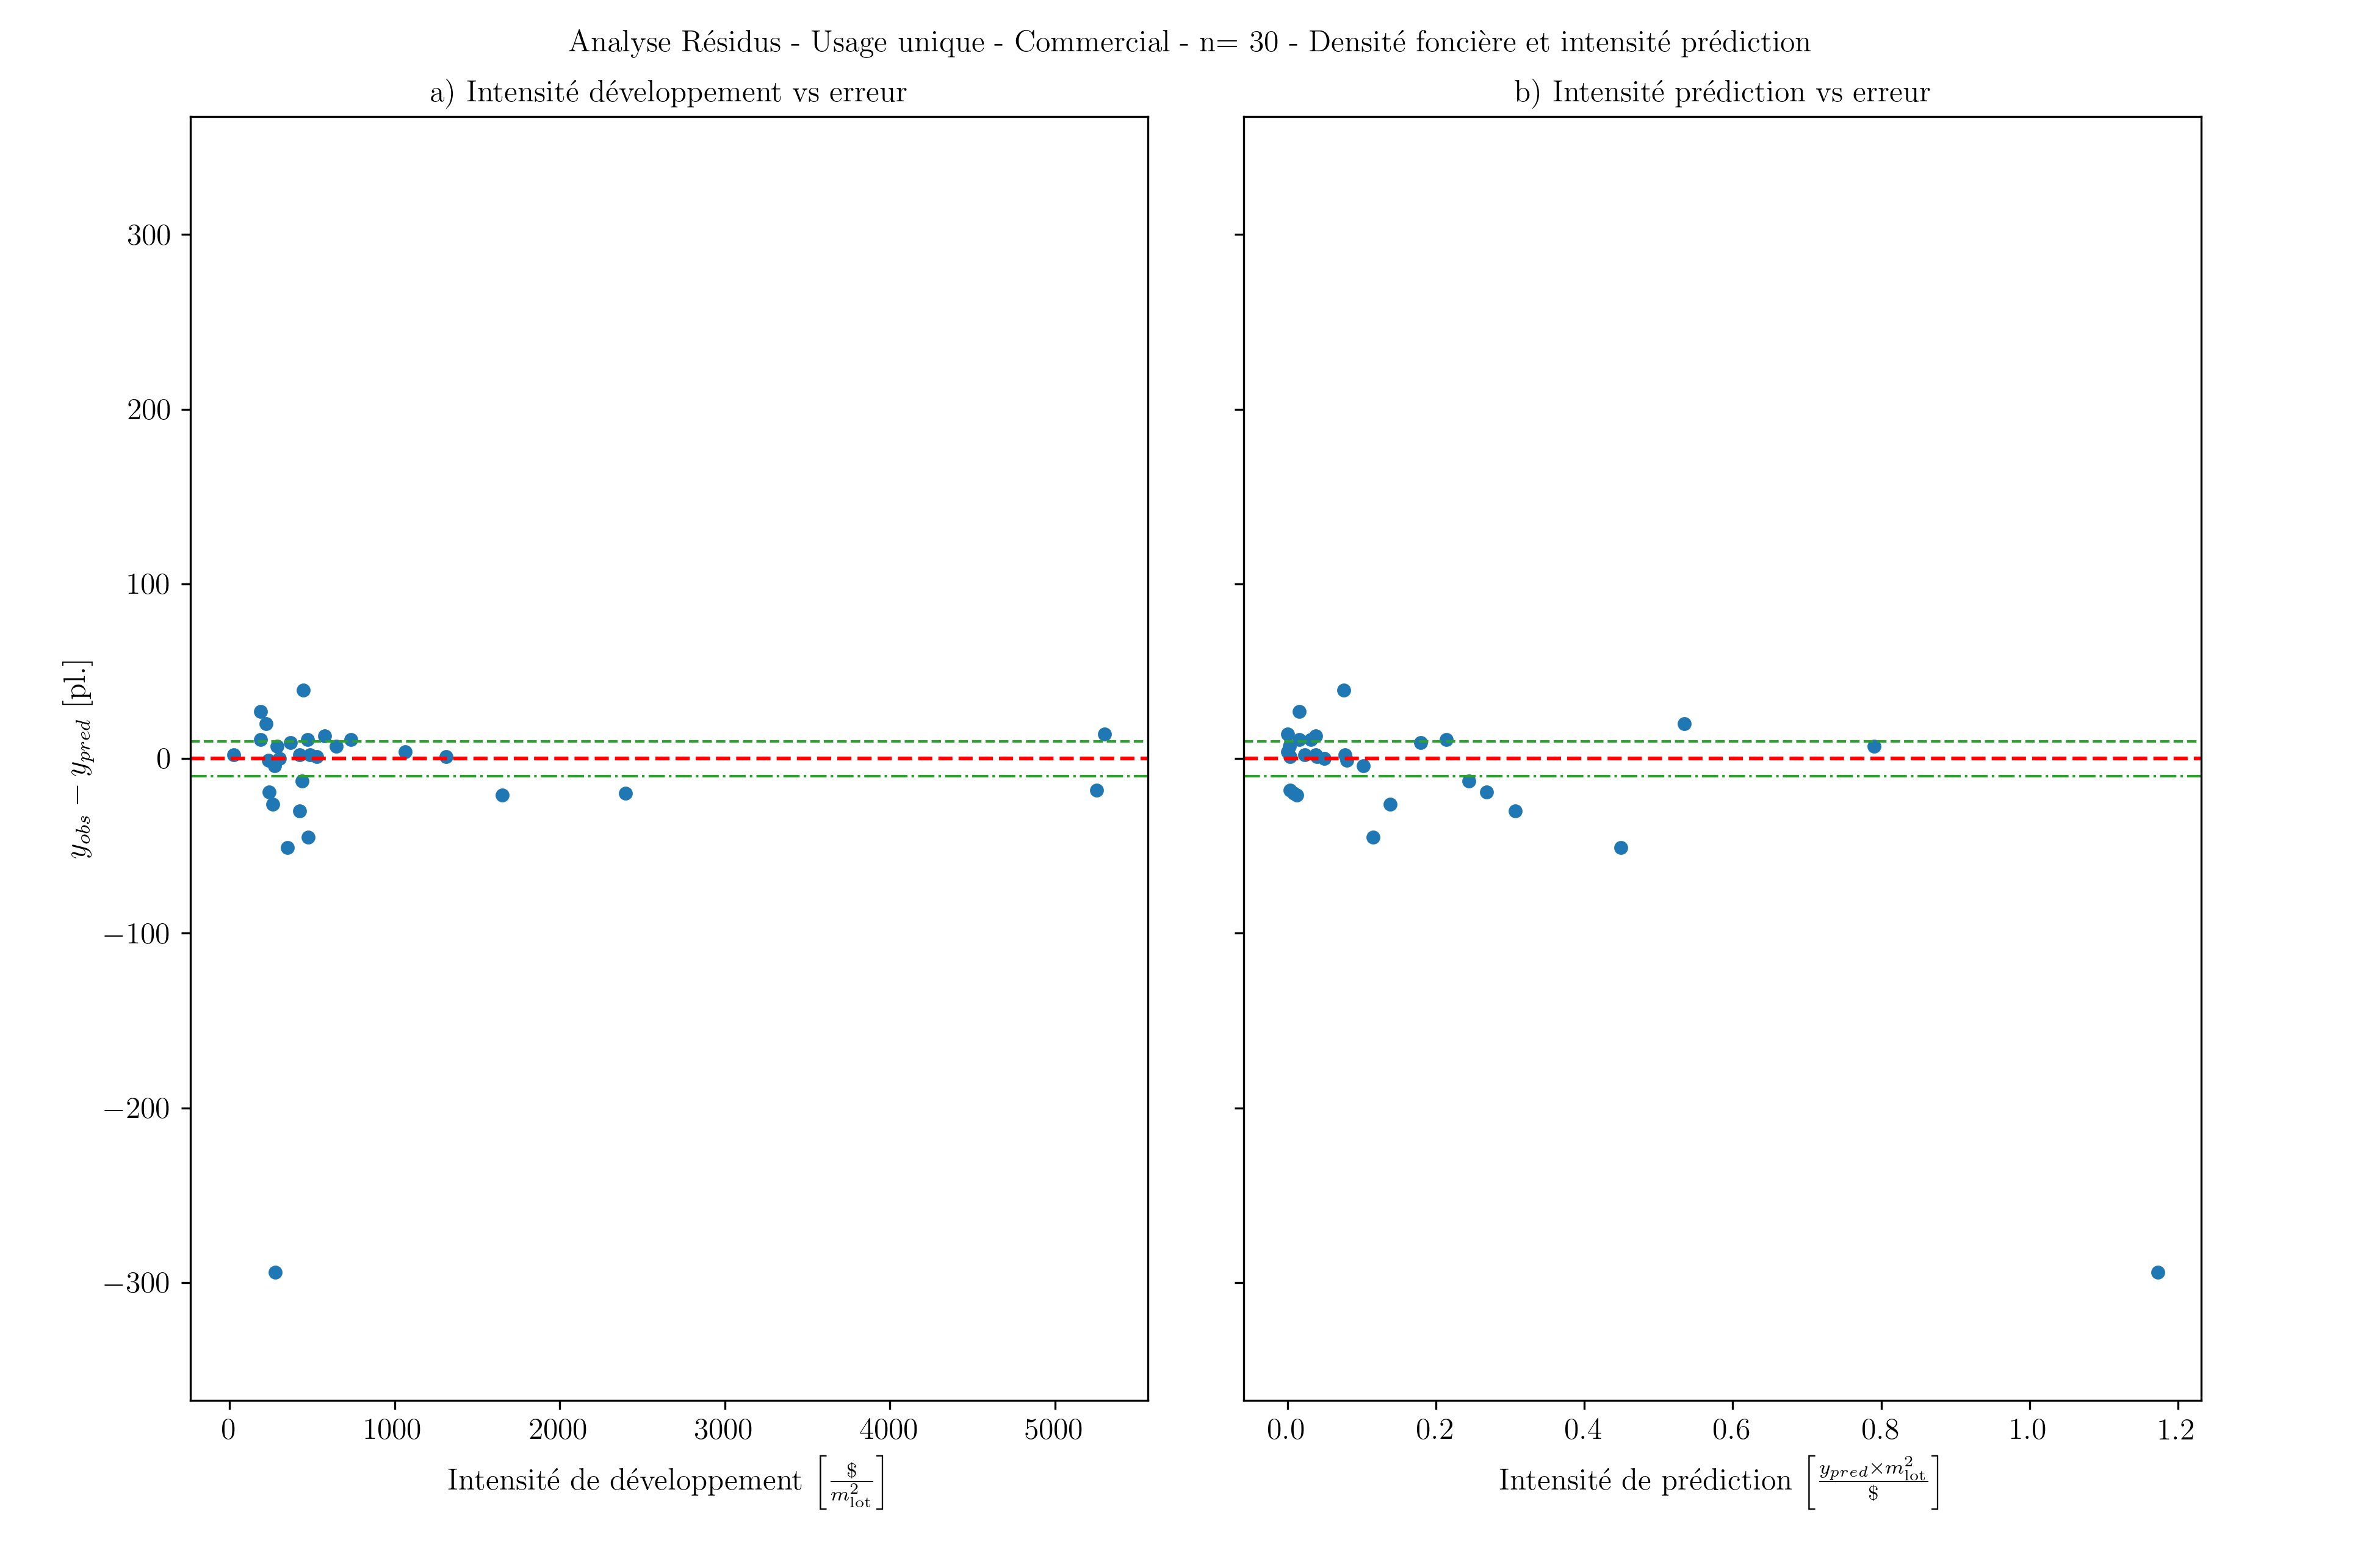
\includegraphics[width=1\linewidth]{images/ana_res_40_se_10_pe_20_e.png}
        \caption{Analyse des résidus en fonction de l'intensité de développement et l'intensité de prédiction pour les lots commerciaux}
        \label{fig:ana-res-intens-comm}
    \end{figure}
\end{landscape}
\subsection{Services}
Trente propriétés de services ont été échantillonnées sur le territoire. Trois lots avec des erreurs supérieurs à 50 ont été éliminés pour les calculs des métriques. Ils peuvent être identifiés à l'aide de la même métrique d'intensité de prédiction montrée à la figure \ref{fig:ana-res-intens-serv}b. En fixant la métrique d'intensité à 0.1 et 0.15, on peut identifier respectivement 90 et 48 lots avec des surestimations potentielles du nombre de places de stationnement. Les lots tombent dans trois grandes catégories: les immeubles à bureaux multiétagés, des écoles et des centres de tri postal. Une fois les grandes erreurs filtrées, le modèle surestime encore le stationnement ($\bar{y}_{obs} = 16.5$ vs $\bar{y}_{pred} =19.0$). La figure \ref{fig:ana-res-unit-pred-serv}a montre que l'erreur croît avec la prédiction. Aucune tendance structurelle n'est identifiée sur les variables physiques des bâtiments, outre la métrique d'intensité de prédiction. \par
Finalement, la figure \ref{fig:serv-err-by-unit} montre que les unités requérant une conversion sont aussi un moyen d'identifier les propriétés avec d'importantes erreurs. La conversion de salles utilisées pour les écoles ou les services de santé sont particulièrement problématiques. L'annexe \ref{ann:recerche-inv-par-unite} donne un exemple de requête SQL pour trouver de telles propriétés.

\begin{landscape}
    \begin{figure}[H]
        \centering
        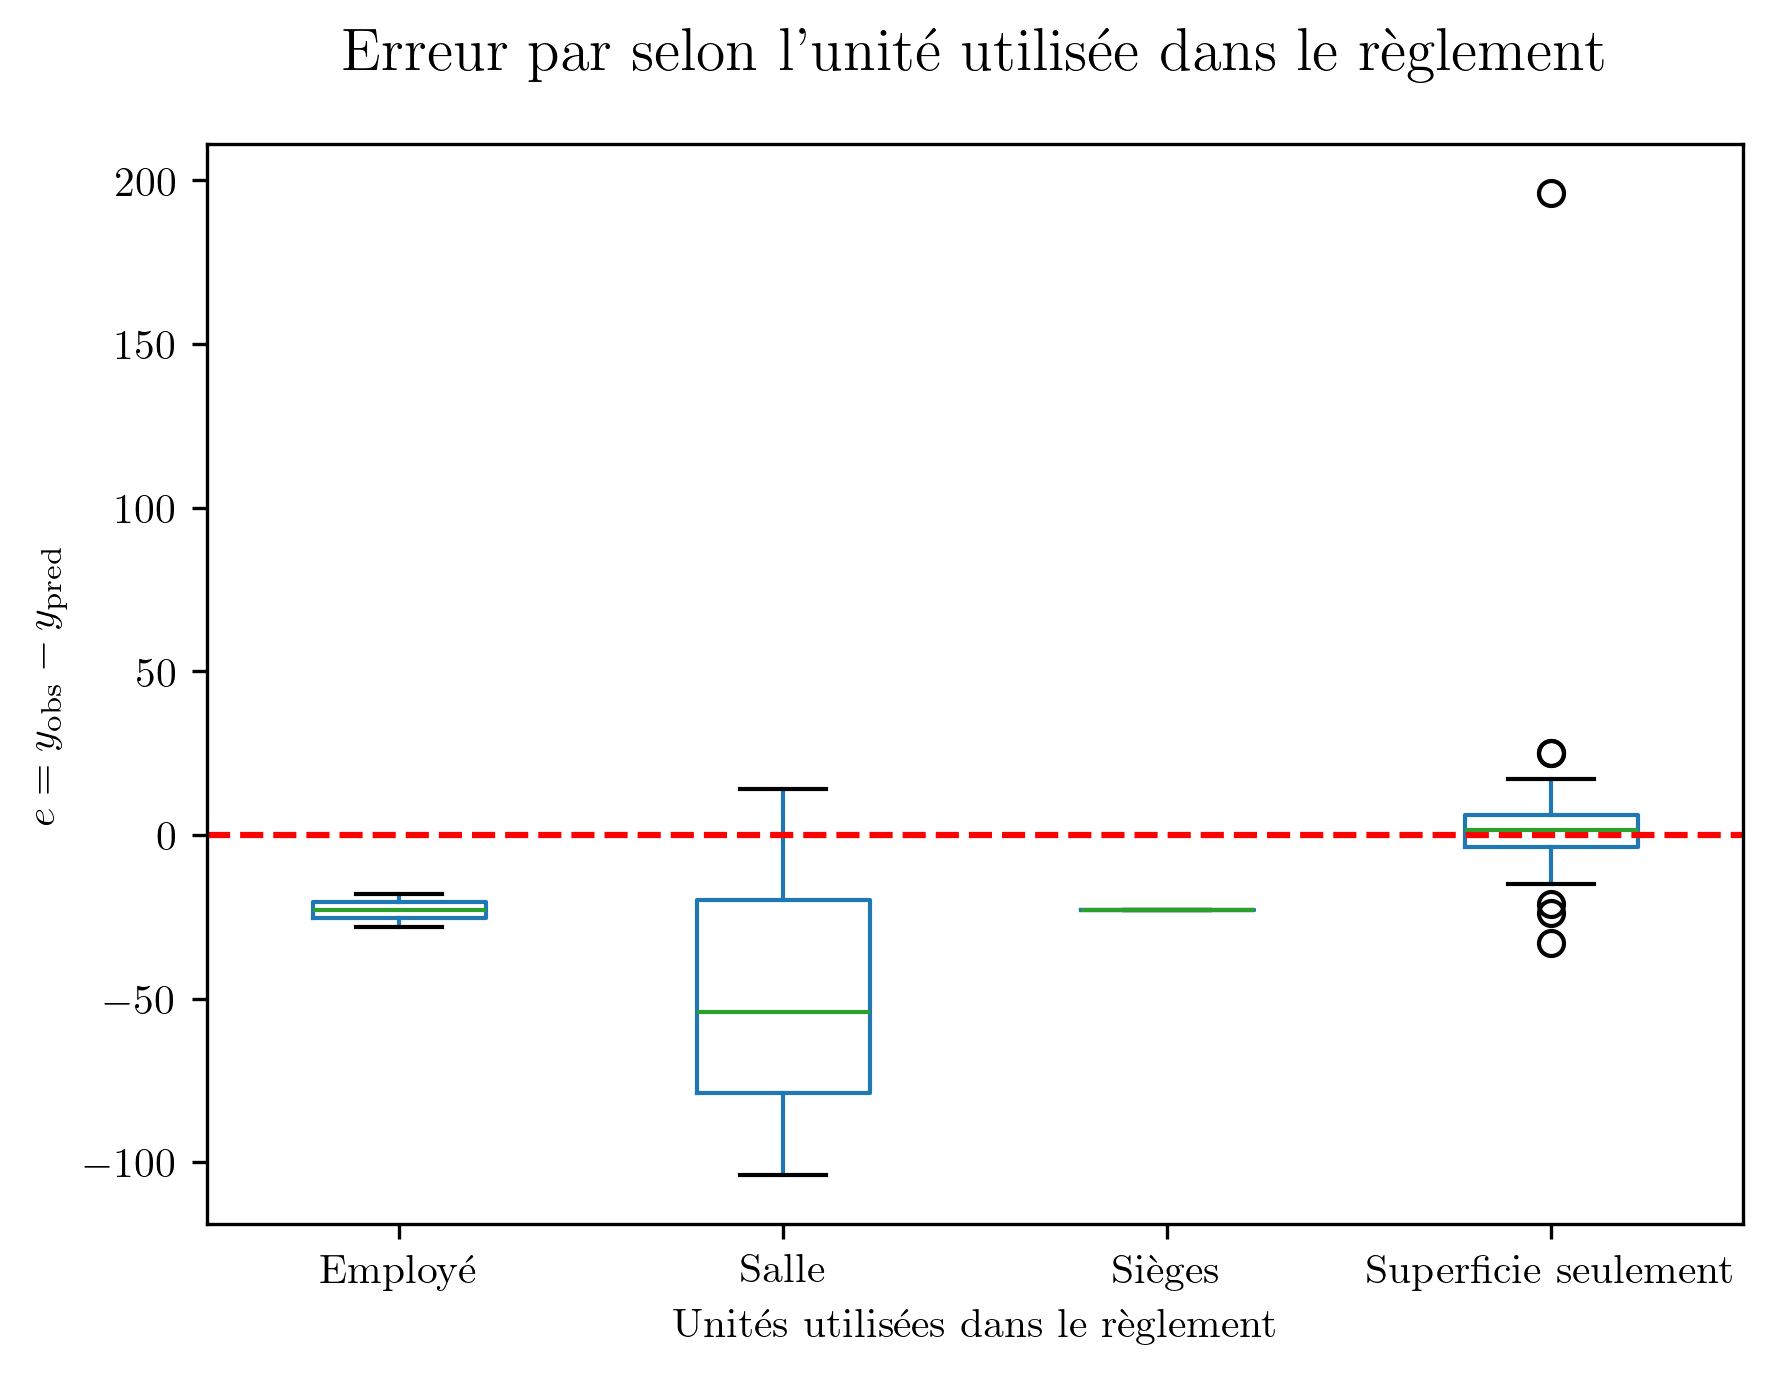
\includegraphics[width=0.8\linewidth]{images/boxplot_error_by_category_41.png}
        \caption{Diagramme à boîte de l'erreur en fonction de l'unité de formulation du règlement pour les services}
        \label{fig:serv-err-by-unit}
    \end{figure}
    %\begin{figure}
    %    \centering
    %    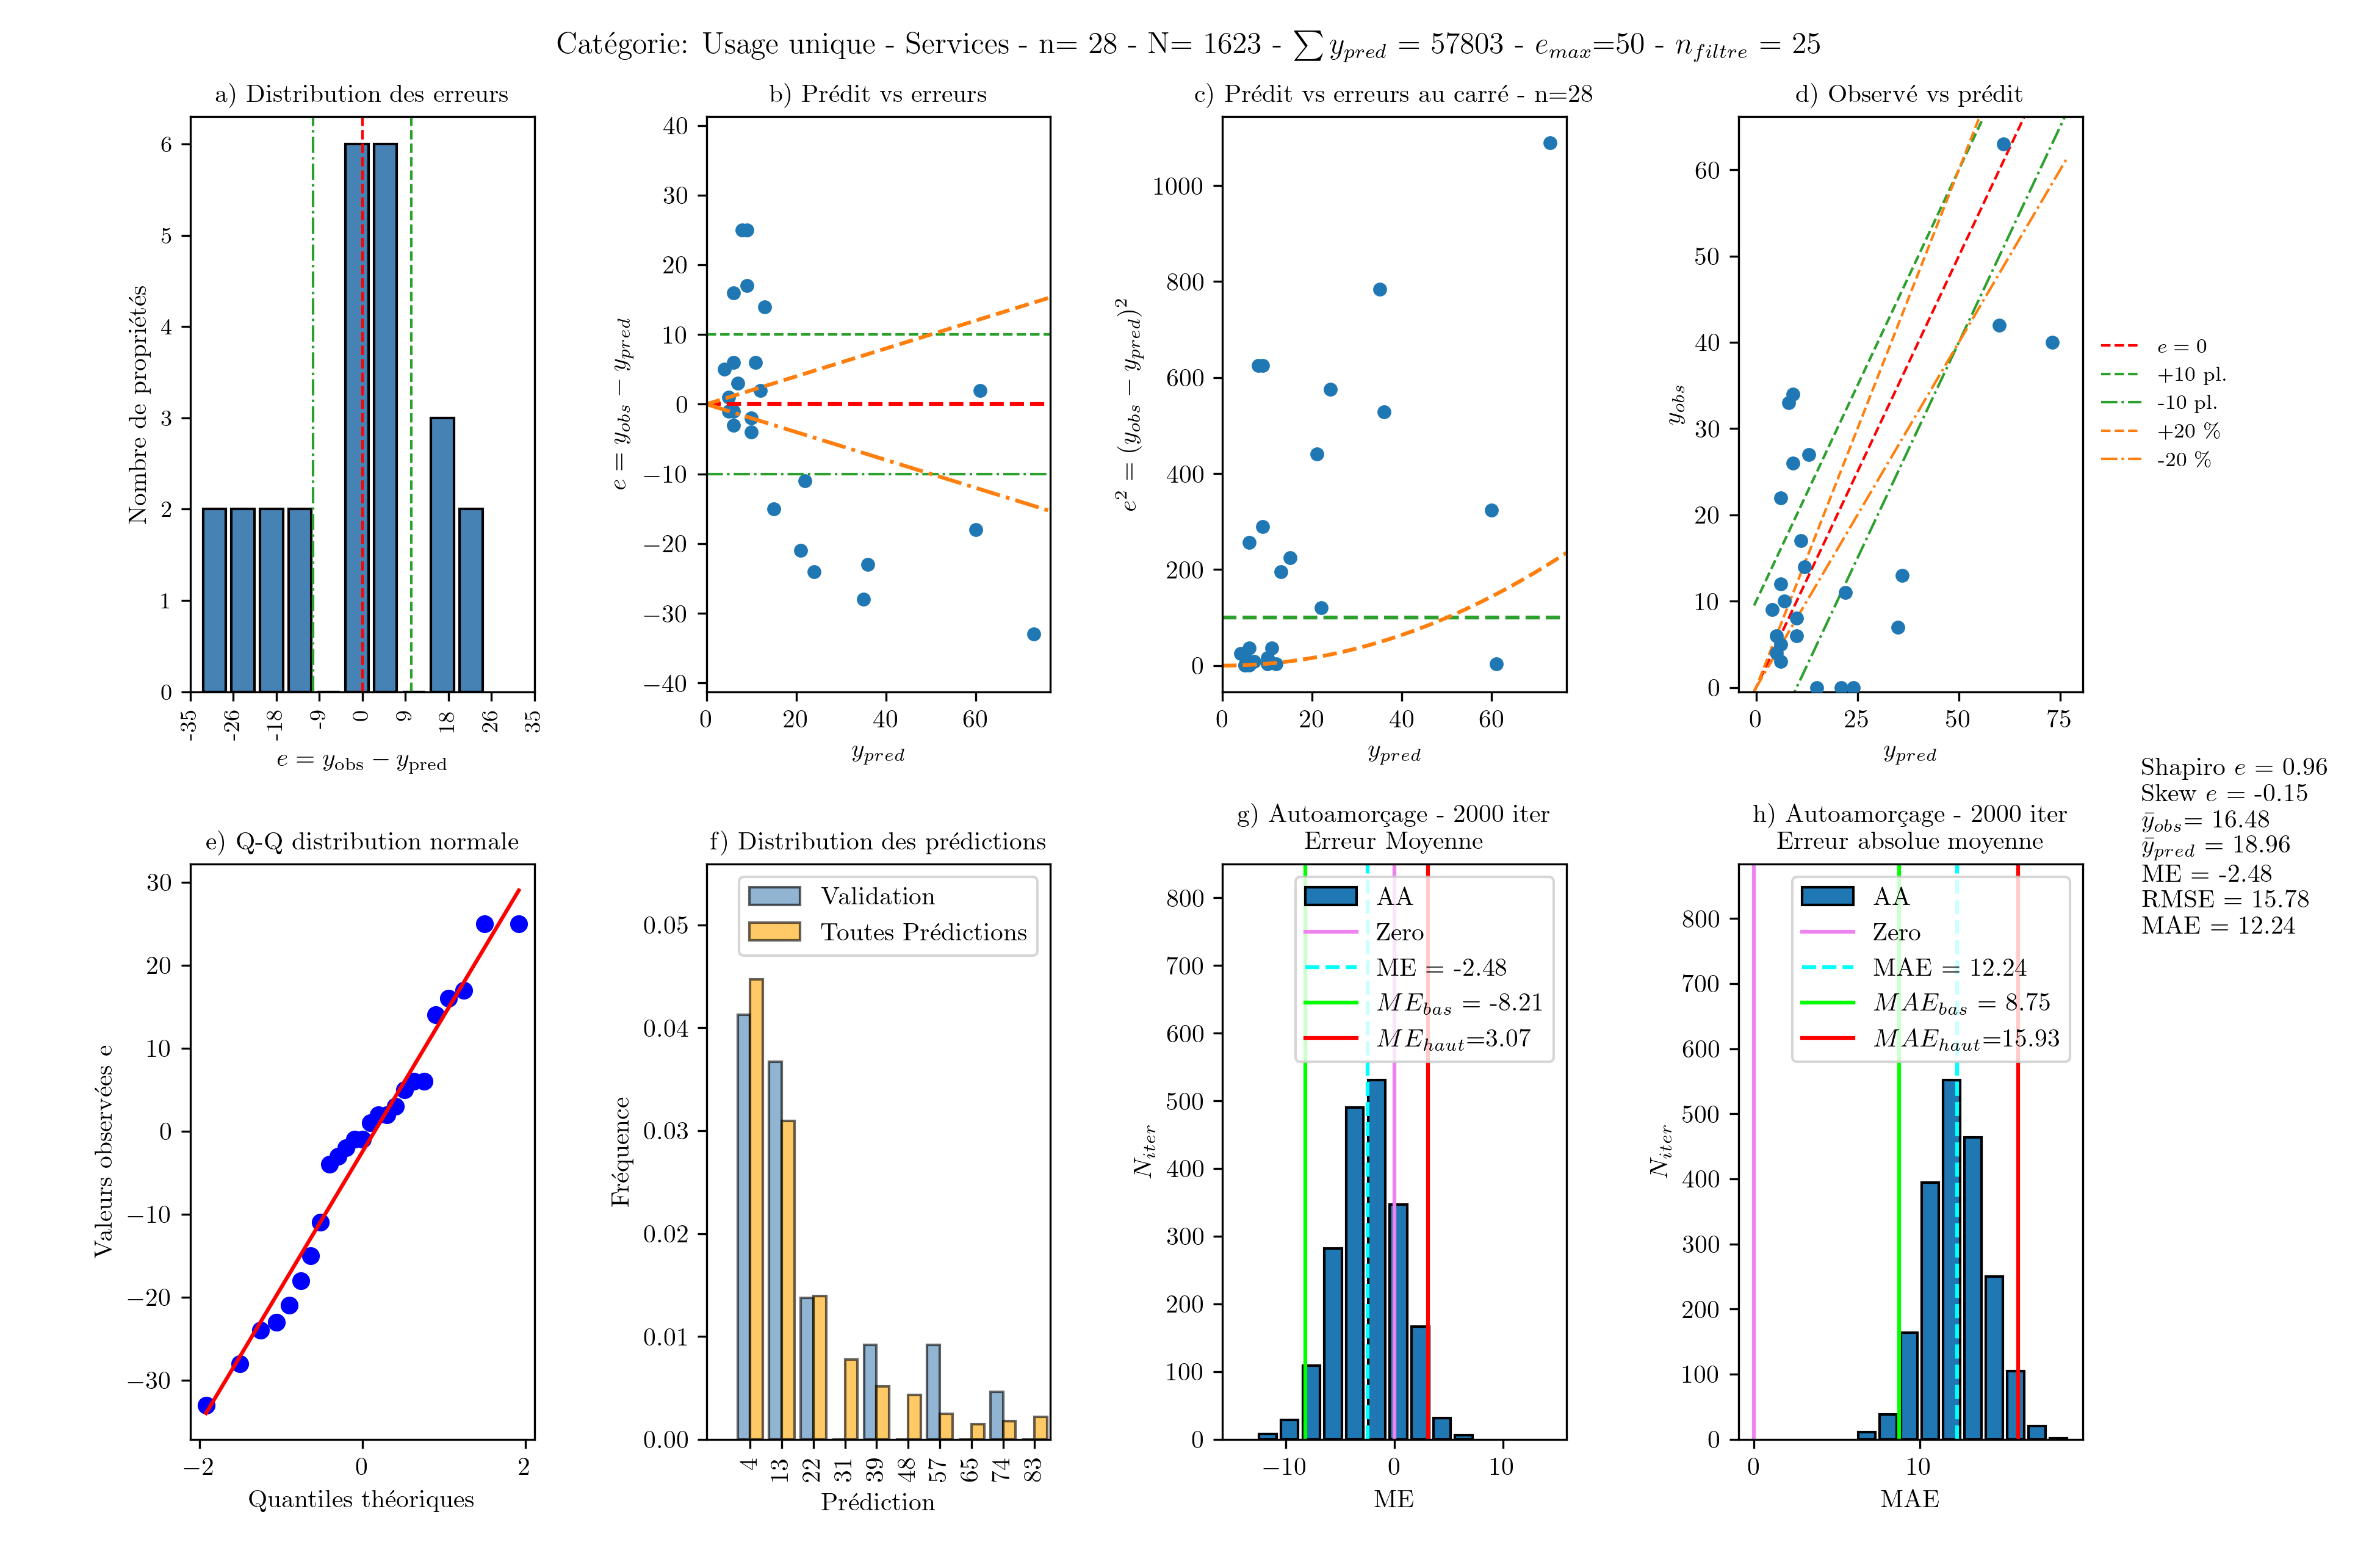
\includegraphics[scale=0.65]{images/int_erreur_41_e_50_se_10_pe_20.png}
    %    \caption{Distribution et intervalles d'erreurs pour les lots de services avec un filtre pour une erreur de %plus de 50 places}
    %    \label{fig:intervals-dis-val-serv-e50}
    %\end{figure}
    \begin{figure}[H]
        \centering
        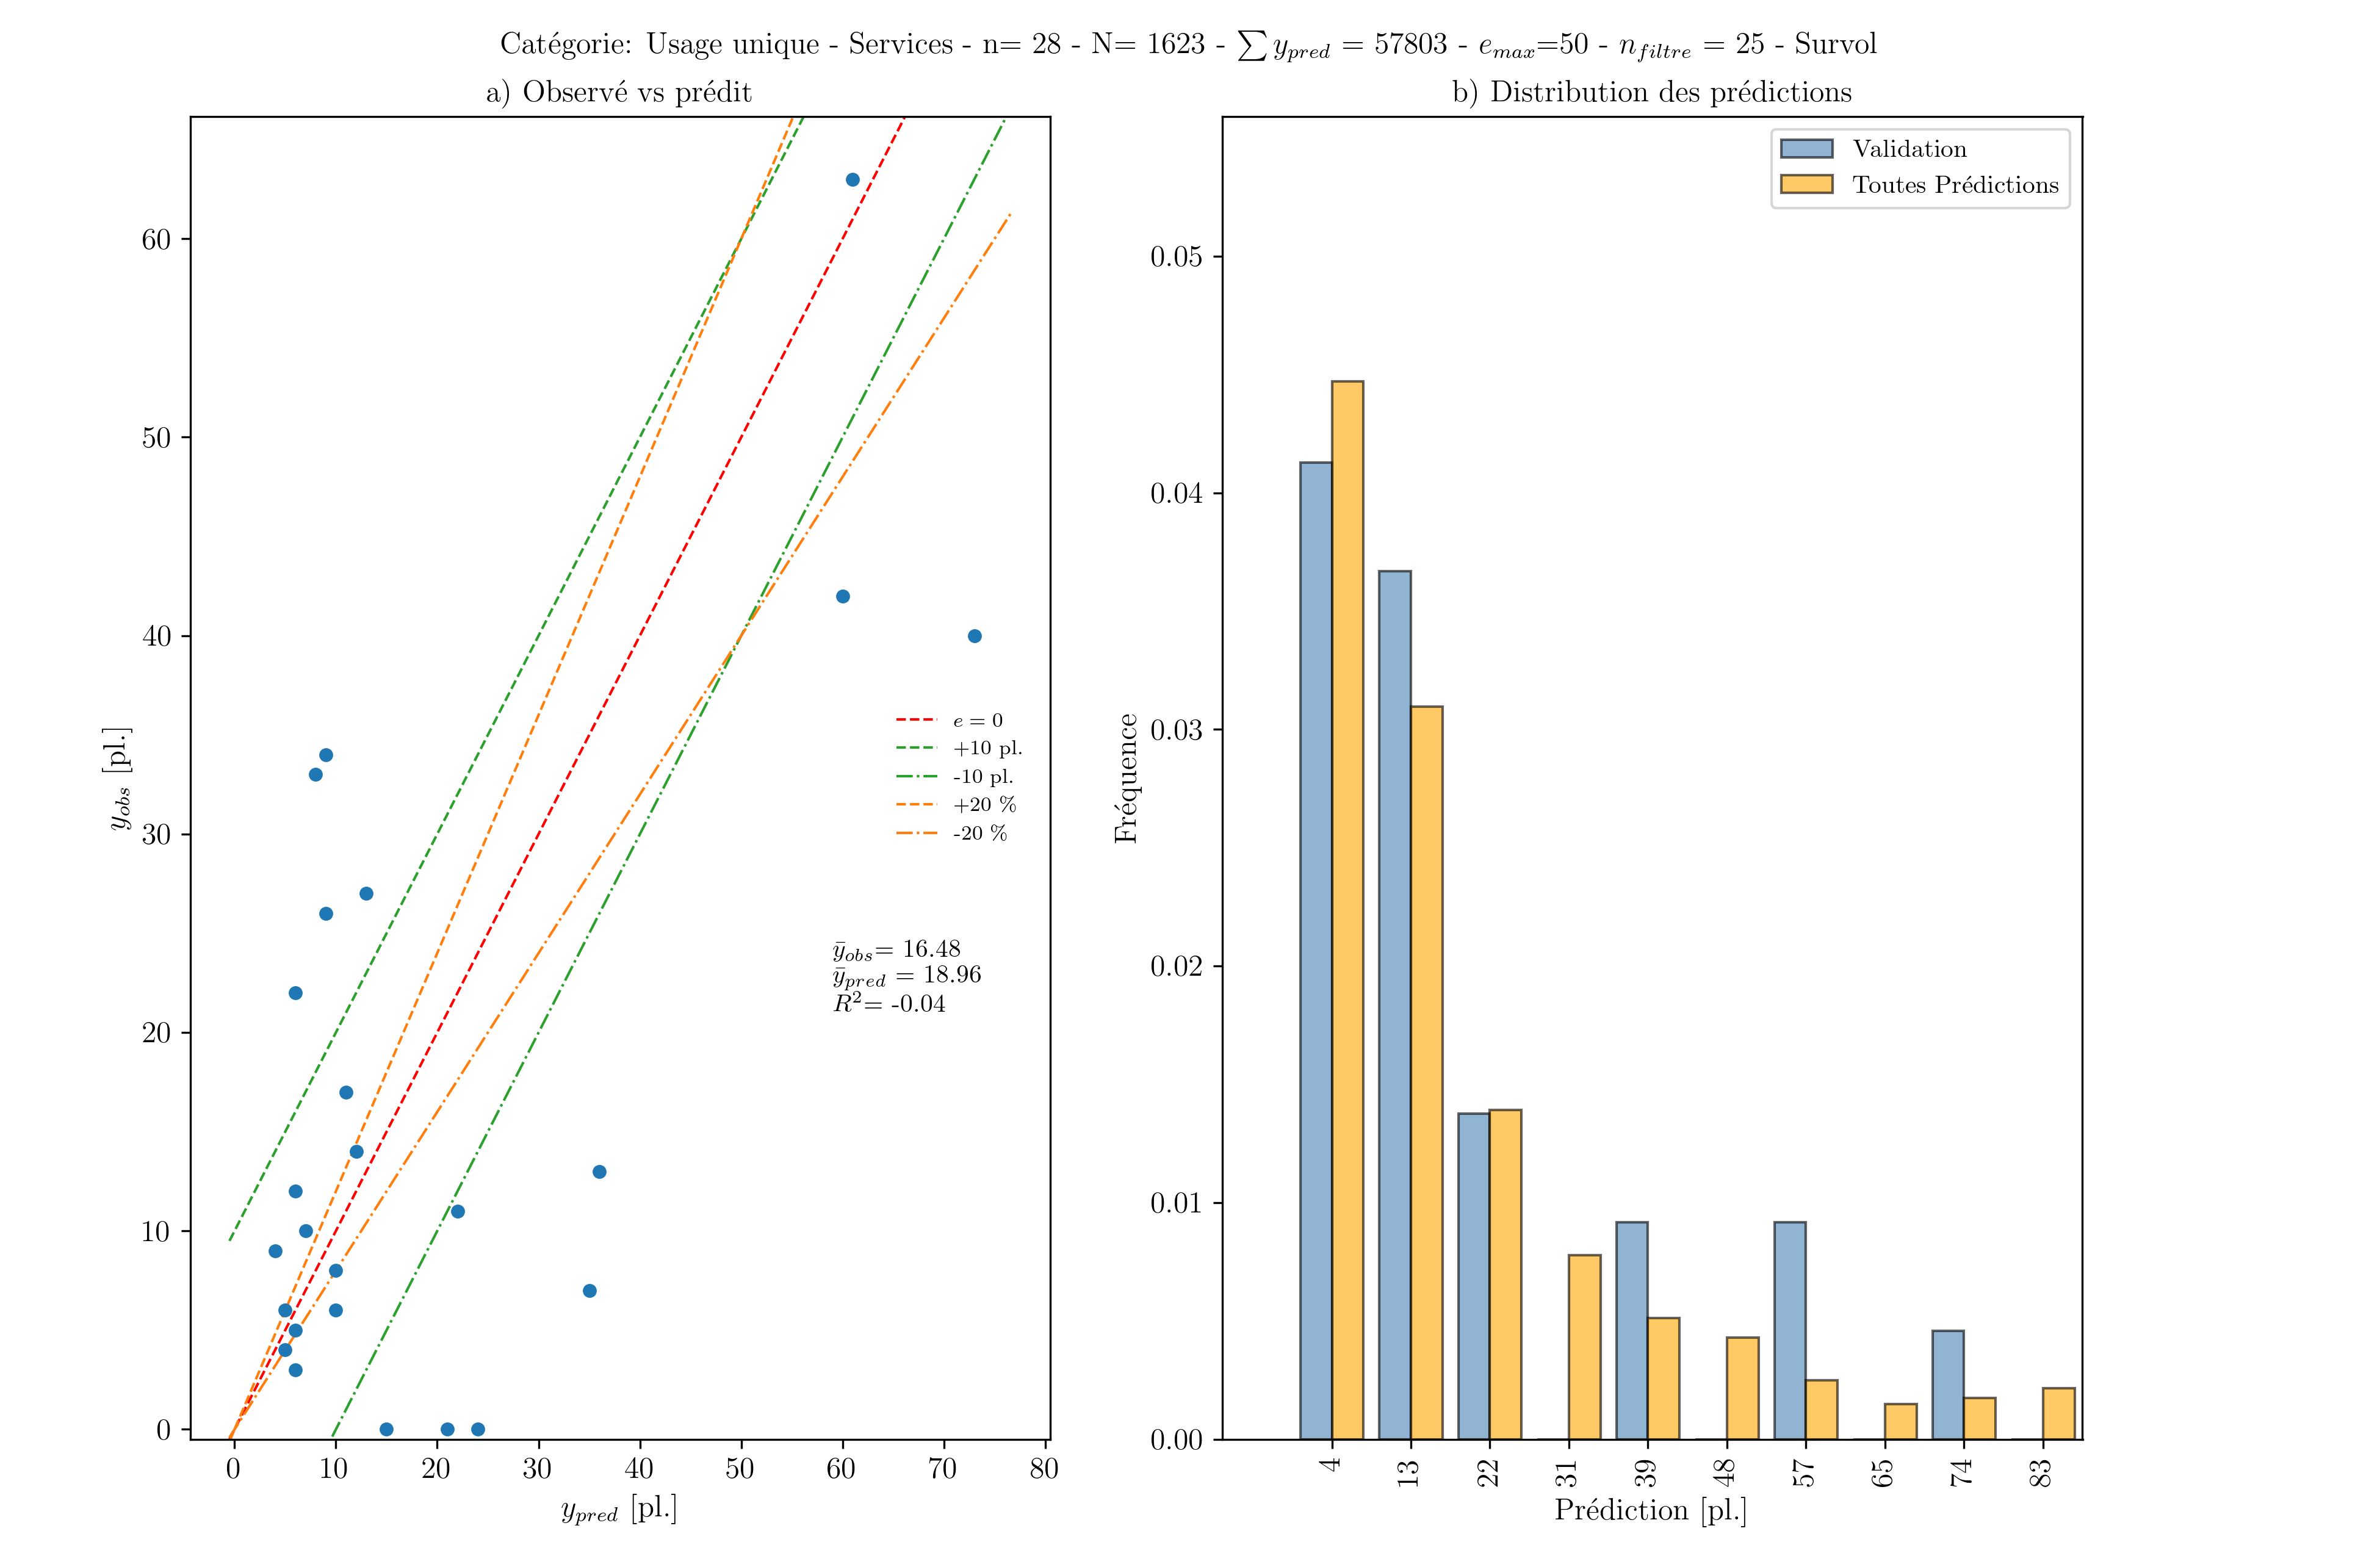
\includegraphics[width=1\linewidth]{images/int_erreur_41_e_50_se_10_pe_20_a.png}
        \caption{Distribution des prédictions pour les lots de services}
        \label{fig:int-dist-pred-serv}
    \end{figure}
    \begin{figure}[H]
        \centering
        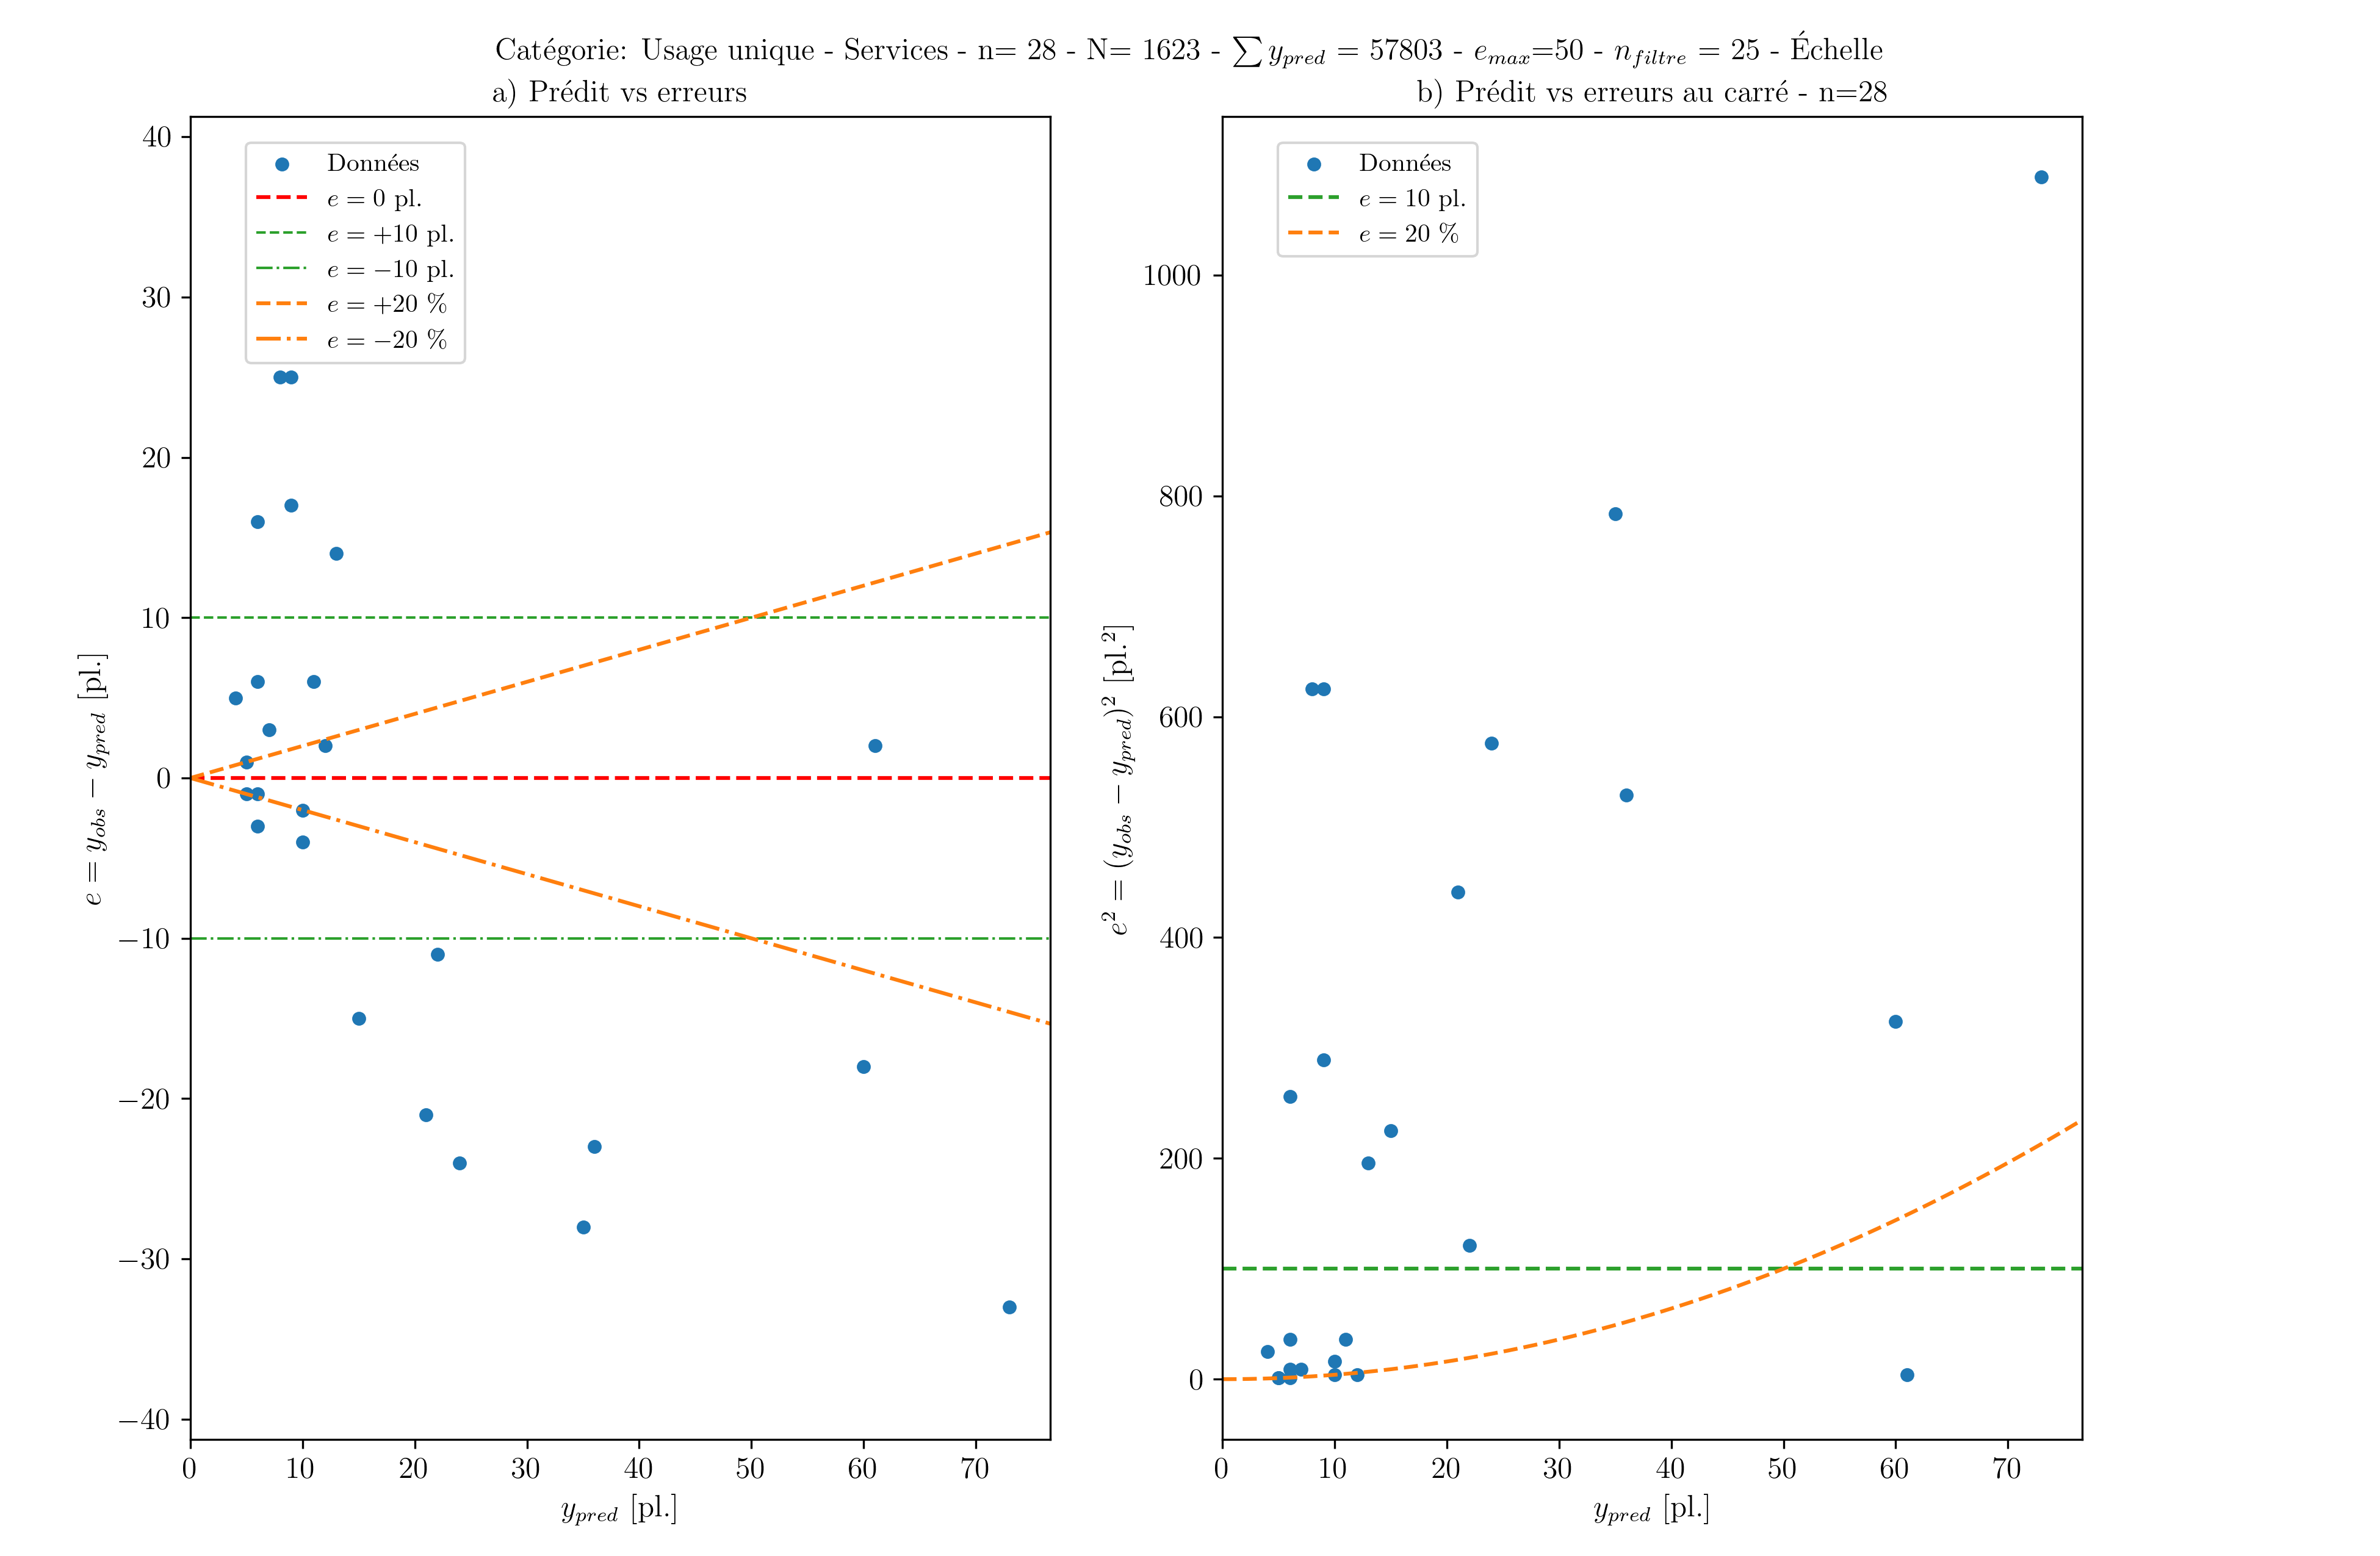
\includegraphics[width=1\linewidth]{images/int_erreur_41_e_50_se_10_pe_20_b.png}
        \caption{Erreur en fonction des prédictions pour les lots de services}
        \label{fig:err-err-quad-pred-serv}
    \end{figure}
    \begin{figure}[H]
        \centering
        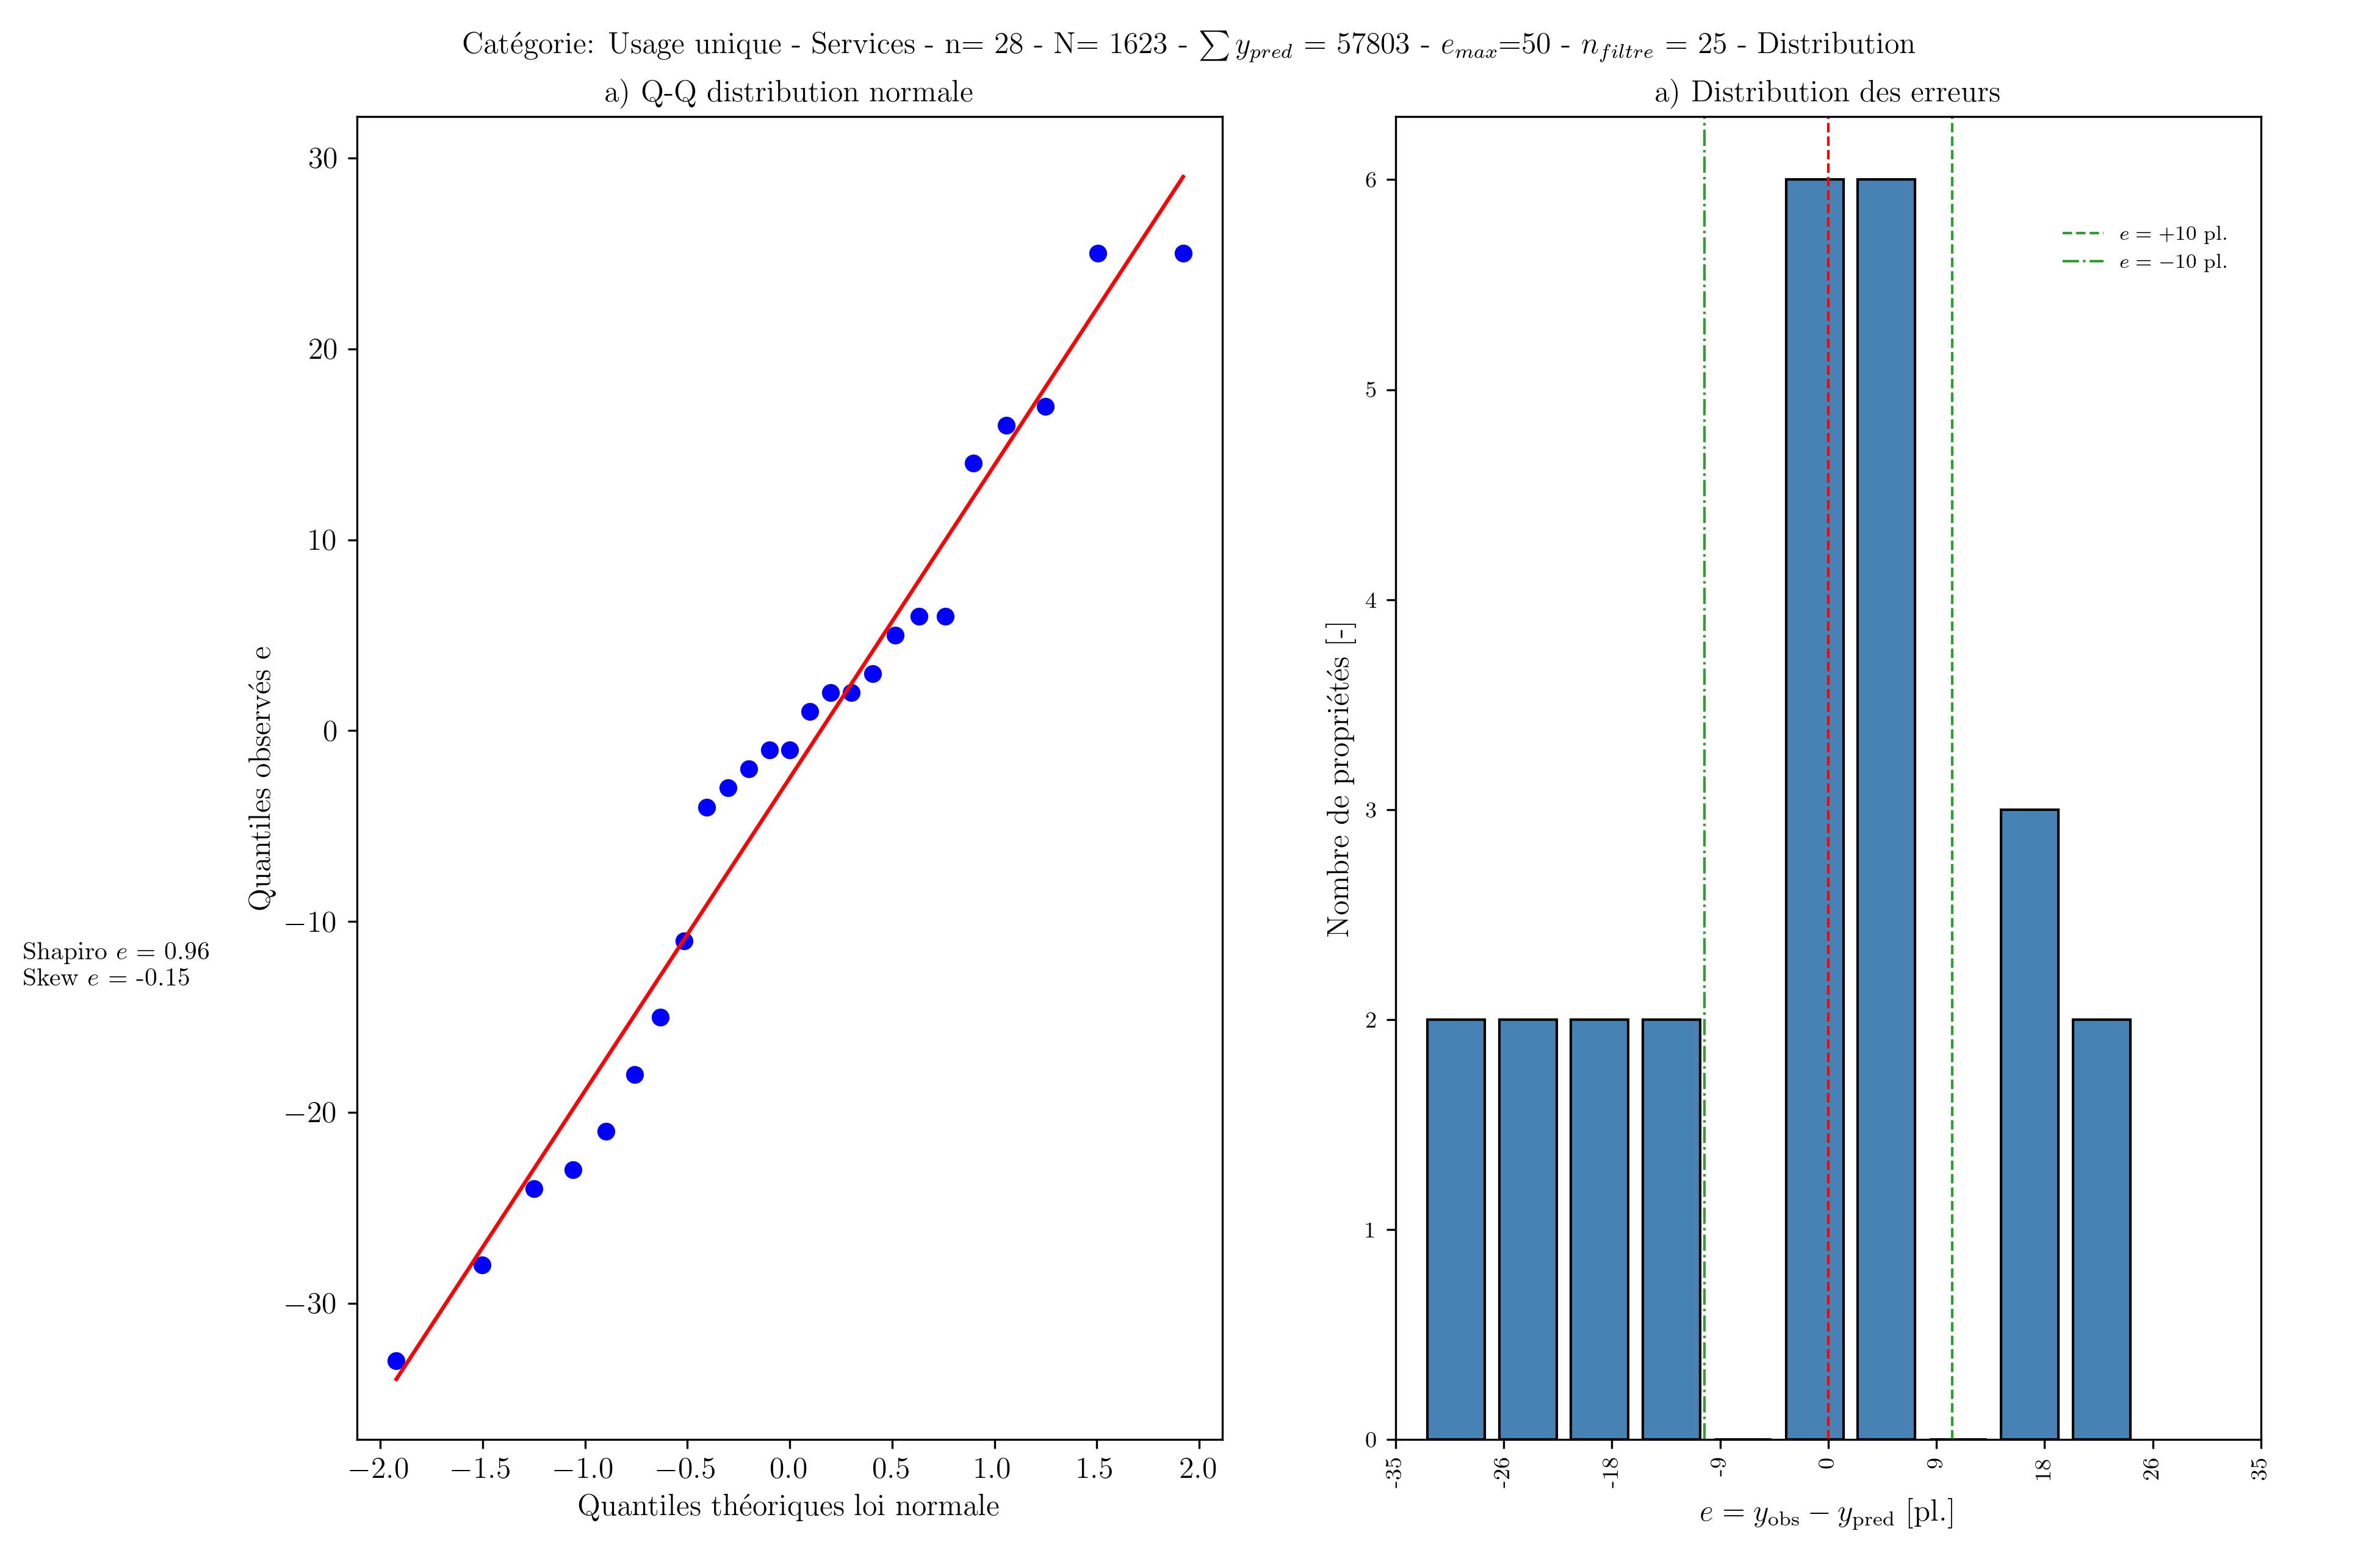
\includegraphics[width=1\linewidth]{images/int_erreur_41_e_50_se_10_pe_20_c.png}
        \caption{Distribution et normalité des erreurs pour les lots de services}
        \label{fig:dist-erreur-norm-serv}
    \end{figure}
    \begin{figure}[H]
        \centering
        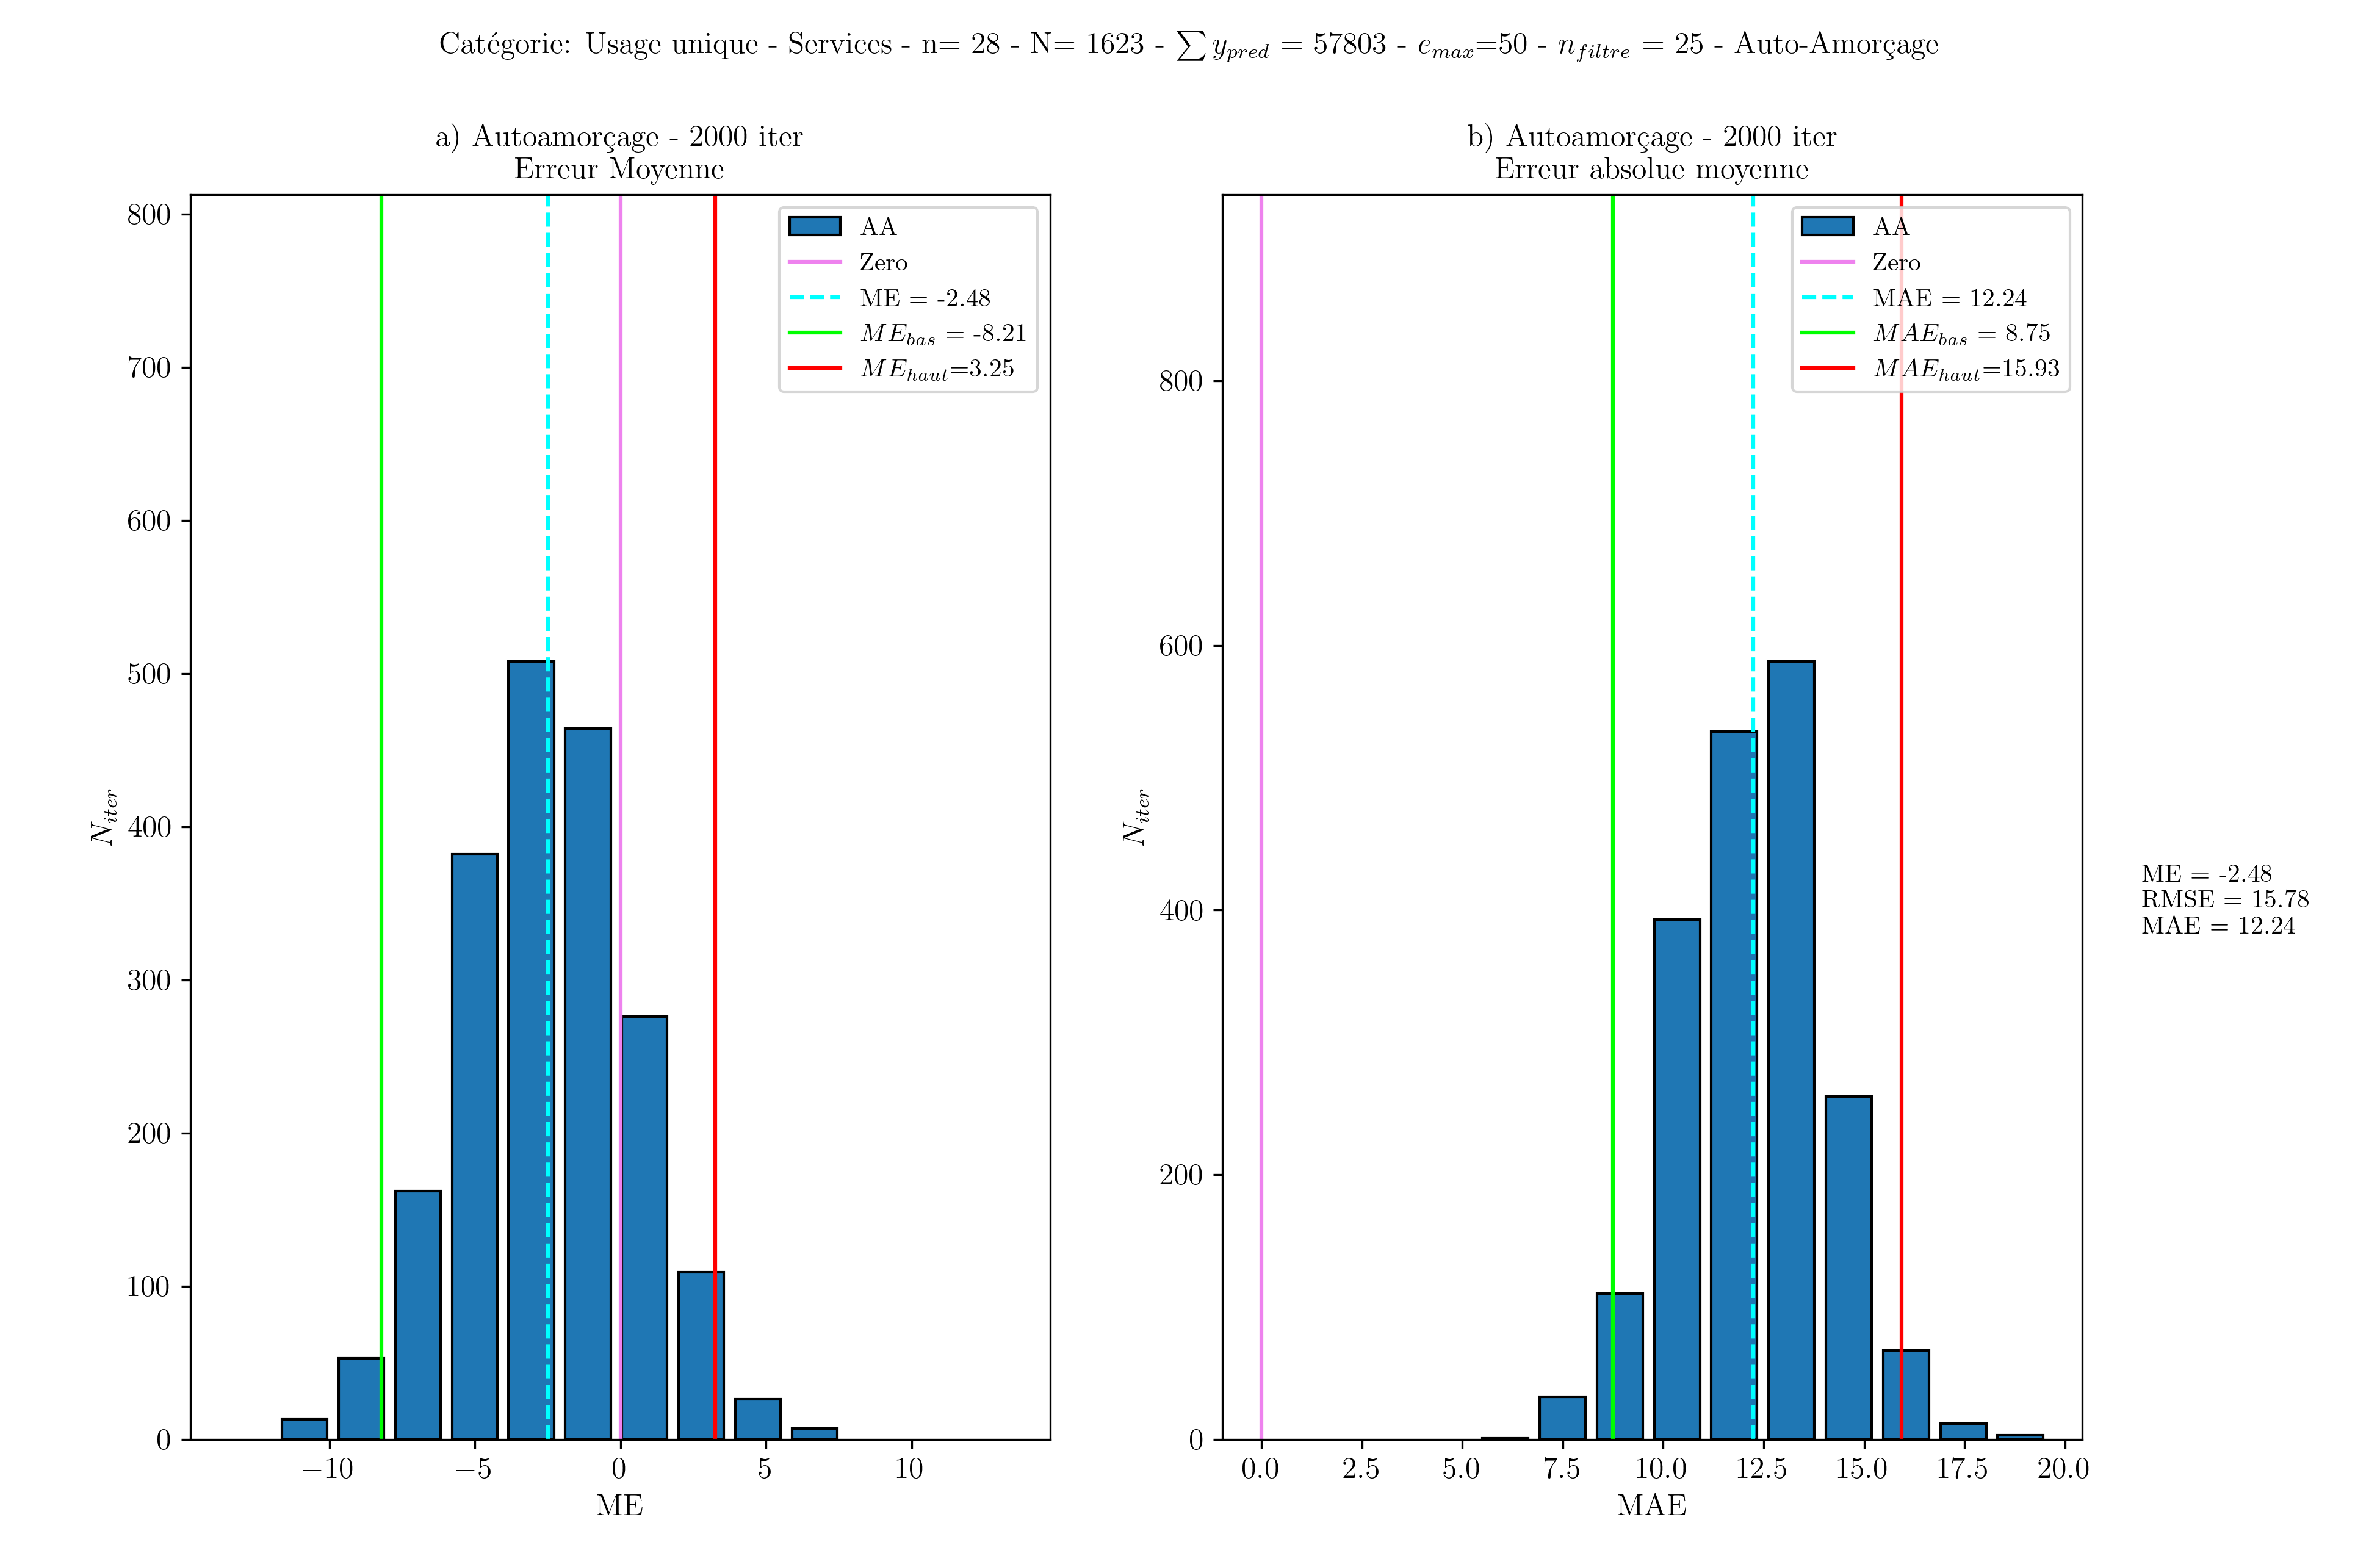
\includegraphics[width=1\linewidth]{images/int_erreur_41_e_50_se_10_pe_20_d.png}
        \caption{Distribution des métriques d'erreur après auto-amorçage pour les lots de services}
        \label{fig:auto-amor-serv}
    \end{figure}
    %\begin{figure}
    %    \centering
    %    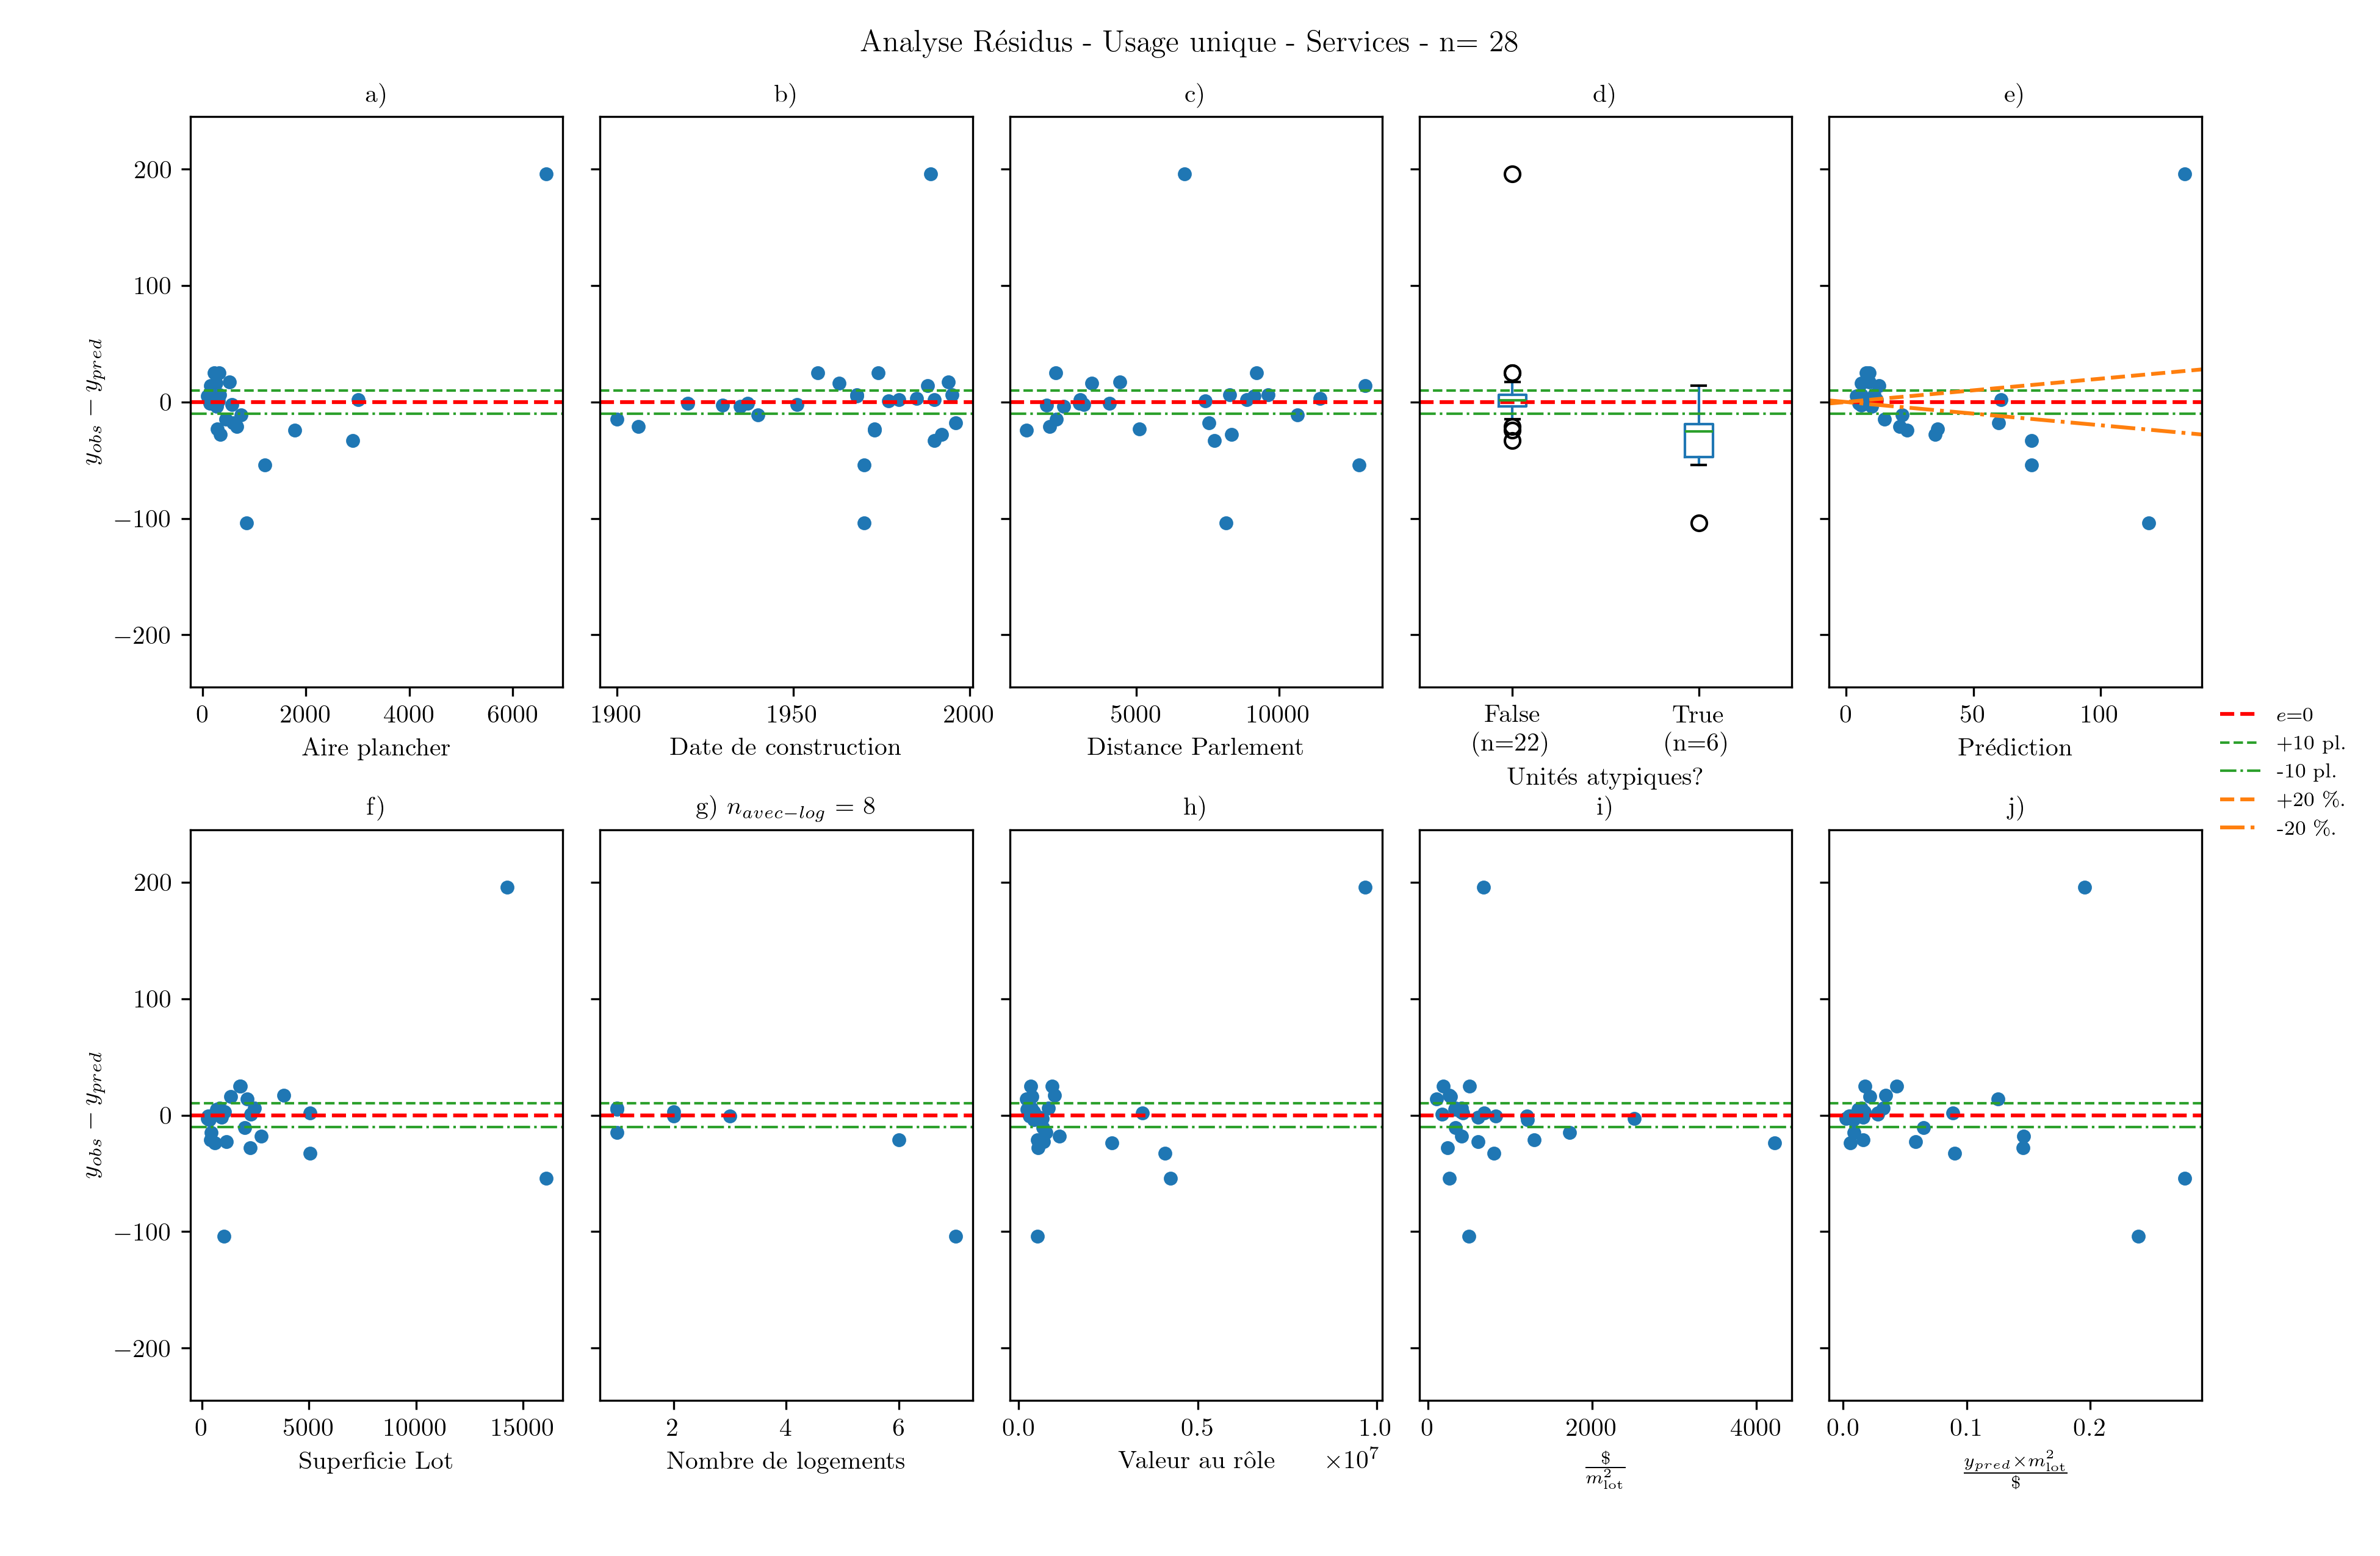
\includegraphics[scale=0.65]{images/ana_res_41_se_10_pe_20.png}
    %    \caption{Analyse des résidus des propriétés de service sans filtre}
    %    \label{fig:ana-residu-serv}
    %\end{figure}
    \begin{figure}[H]
        \centering
        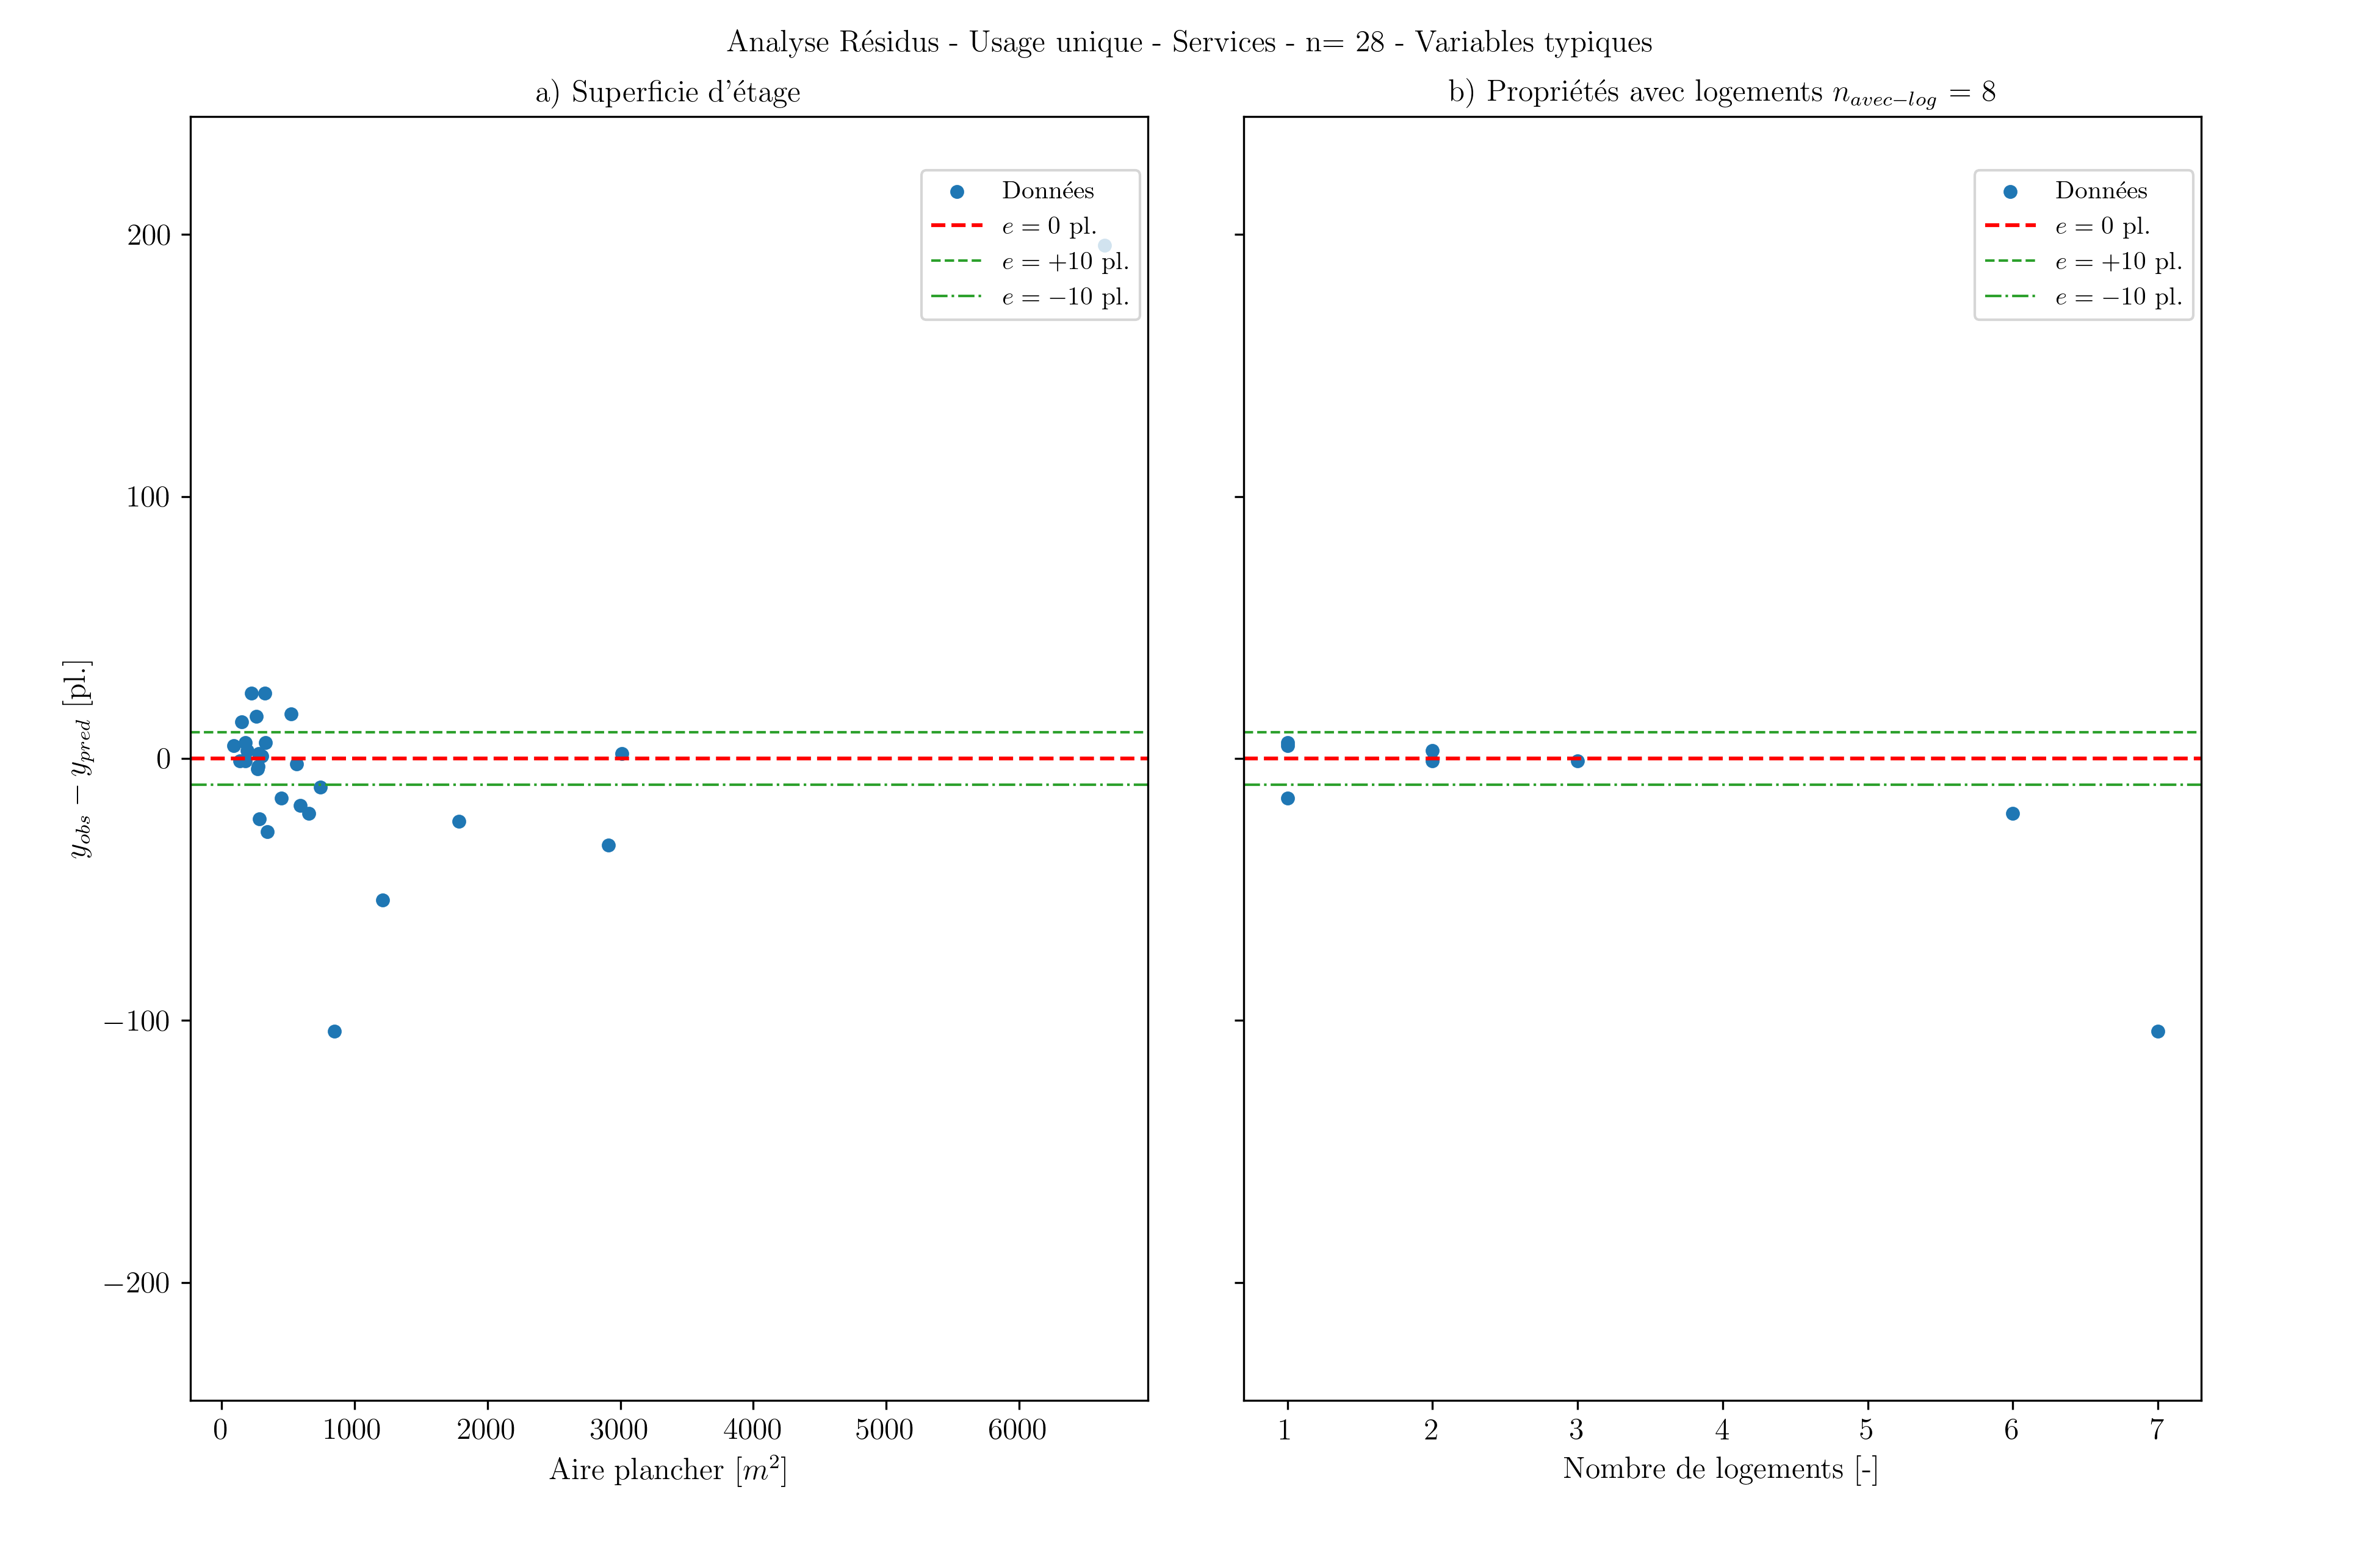
\includegraphics[width=1\linewidth]{images/ana_res_41_se_10_pe_20_a.png}
        \caption{Analyse des résidus en fonction des propriétés de construction pour les lots de services}
        \label{fig:ana-res-prop-phys-serv}
    \end{figure}
    \begin{figure}[H]
        \centering
        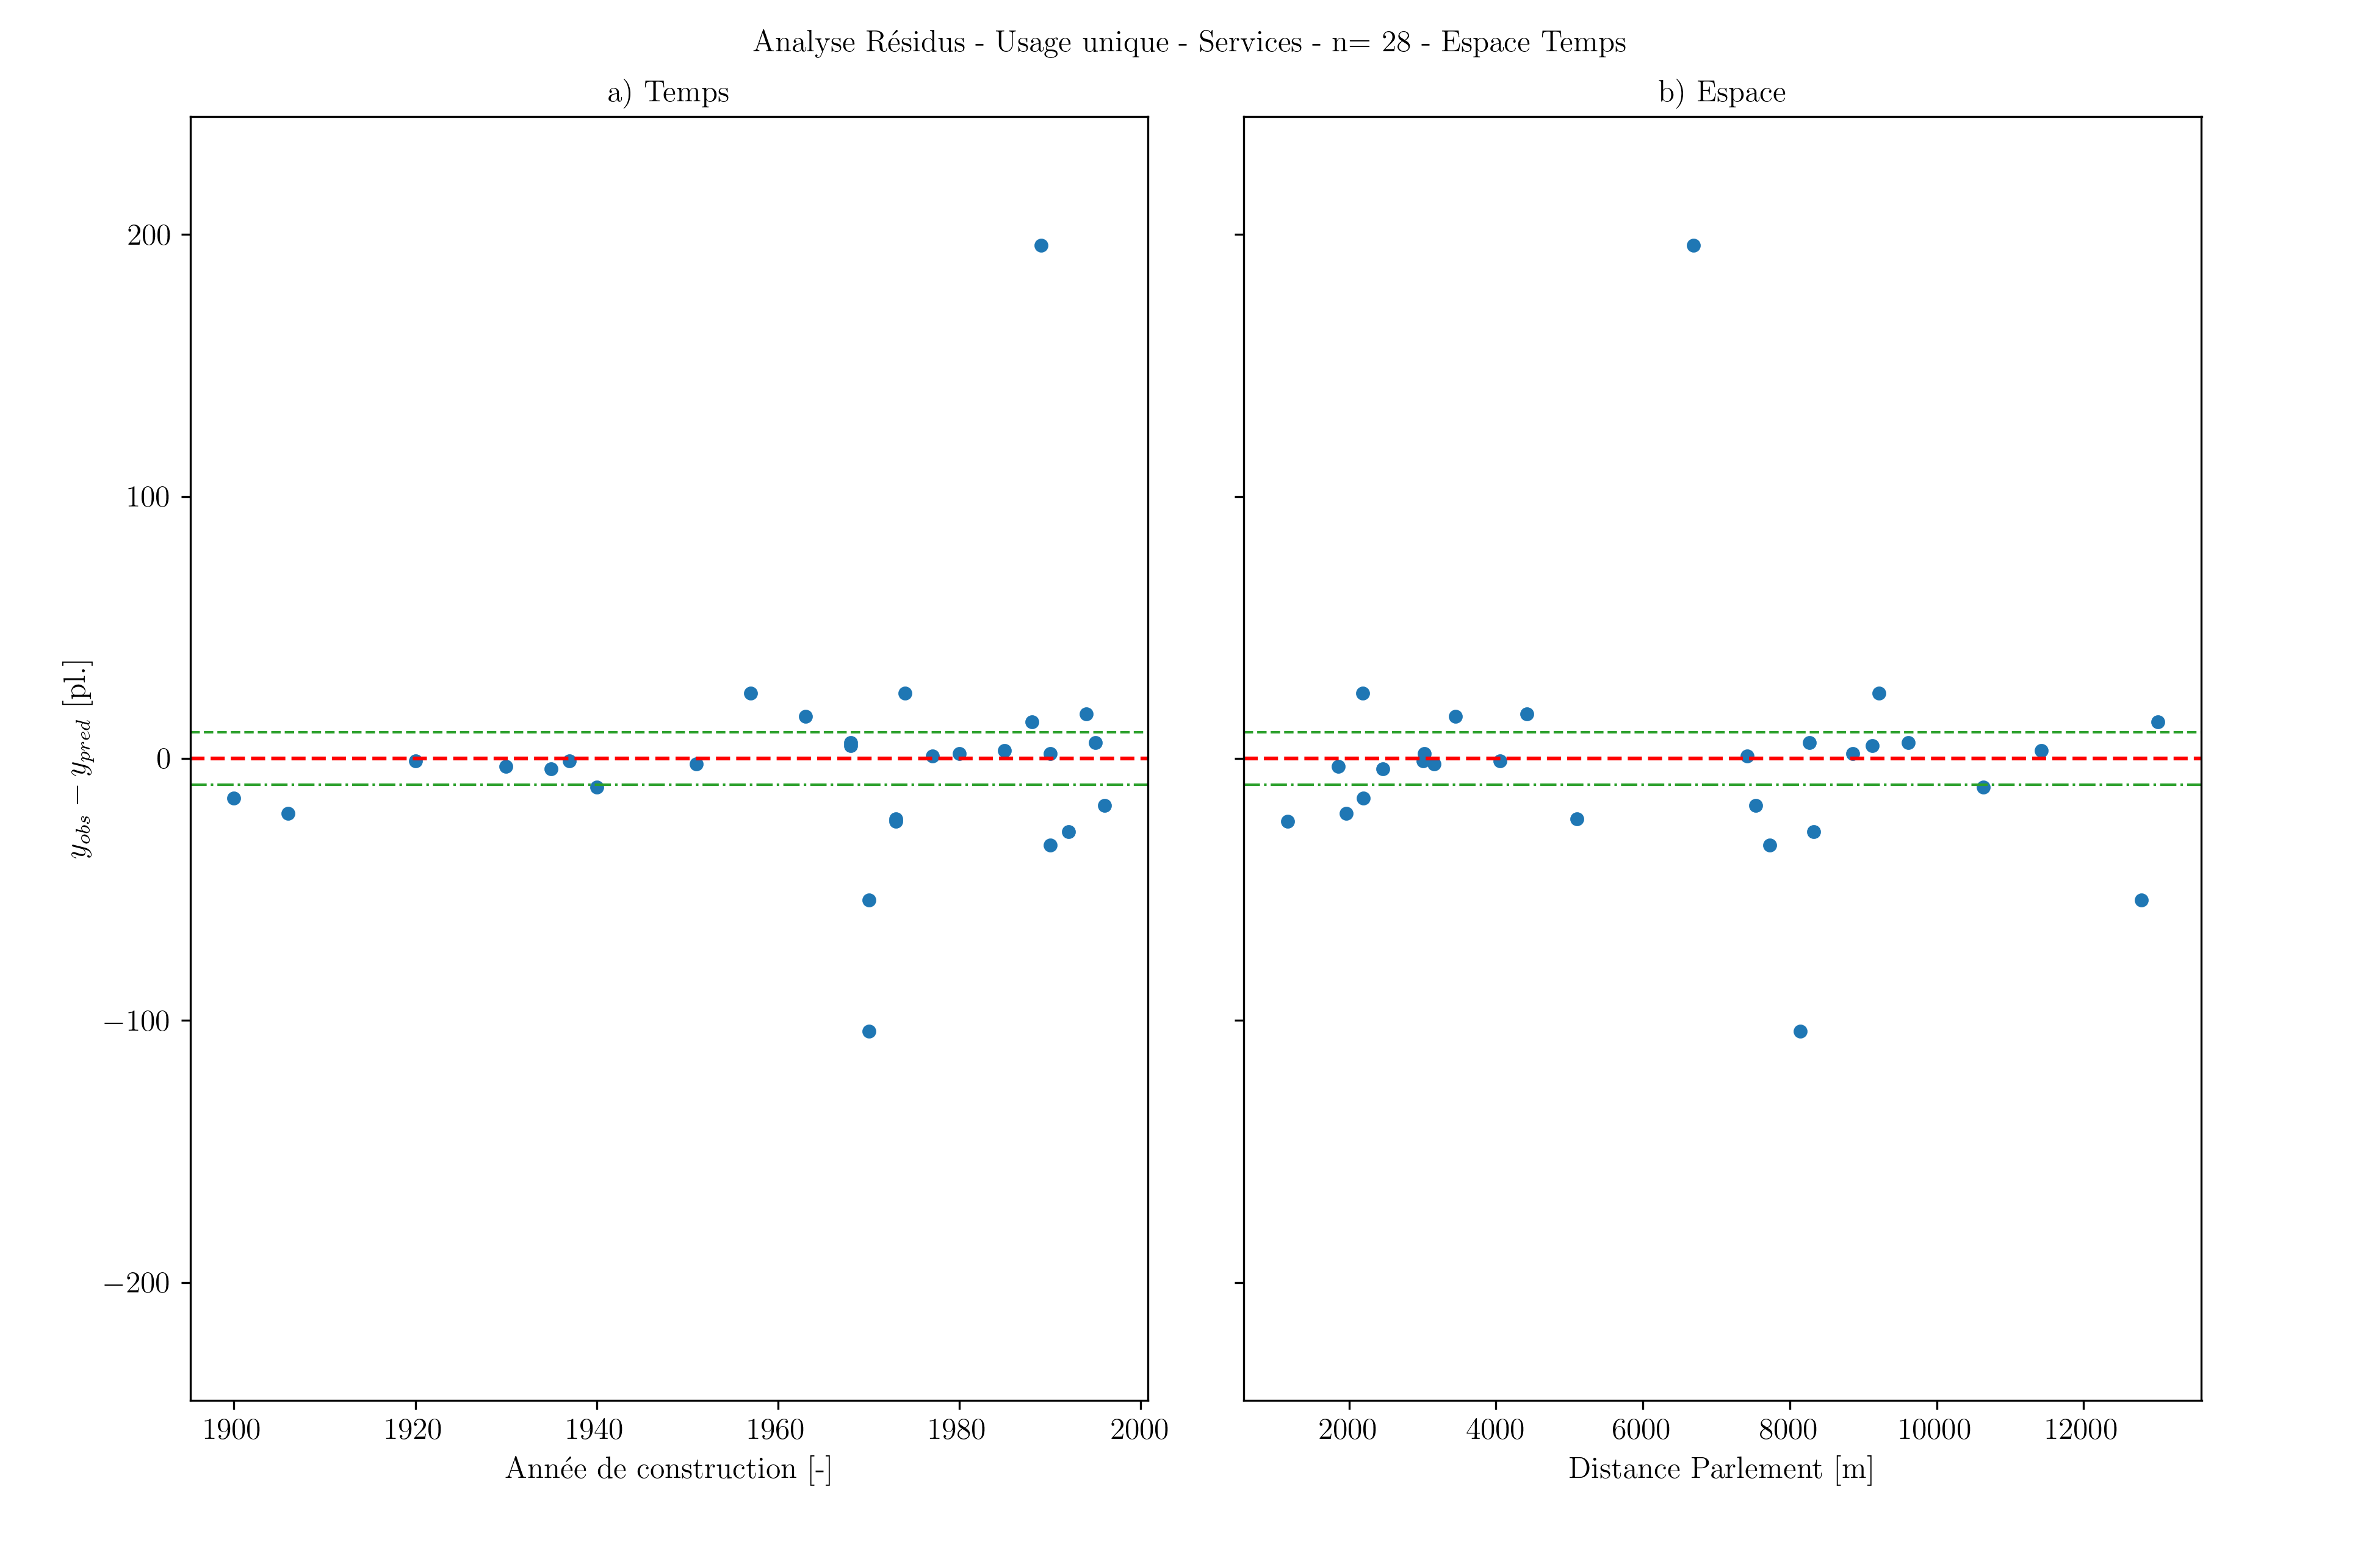
\includegraphics[width=1\linewidth]{images/ana_res_41_se_10_pe_20_b.png}
        \caption{Analyse des résidus en fonction de l'espace et de l'époque de construction pour les lots de services}
        \label{fig:ana-res-esp-temps-serv}
    \end{figure}
    \begin{figure}[H]
        \centering
        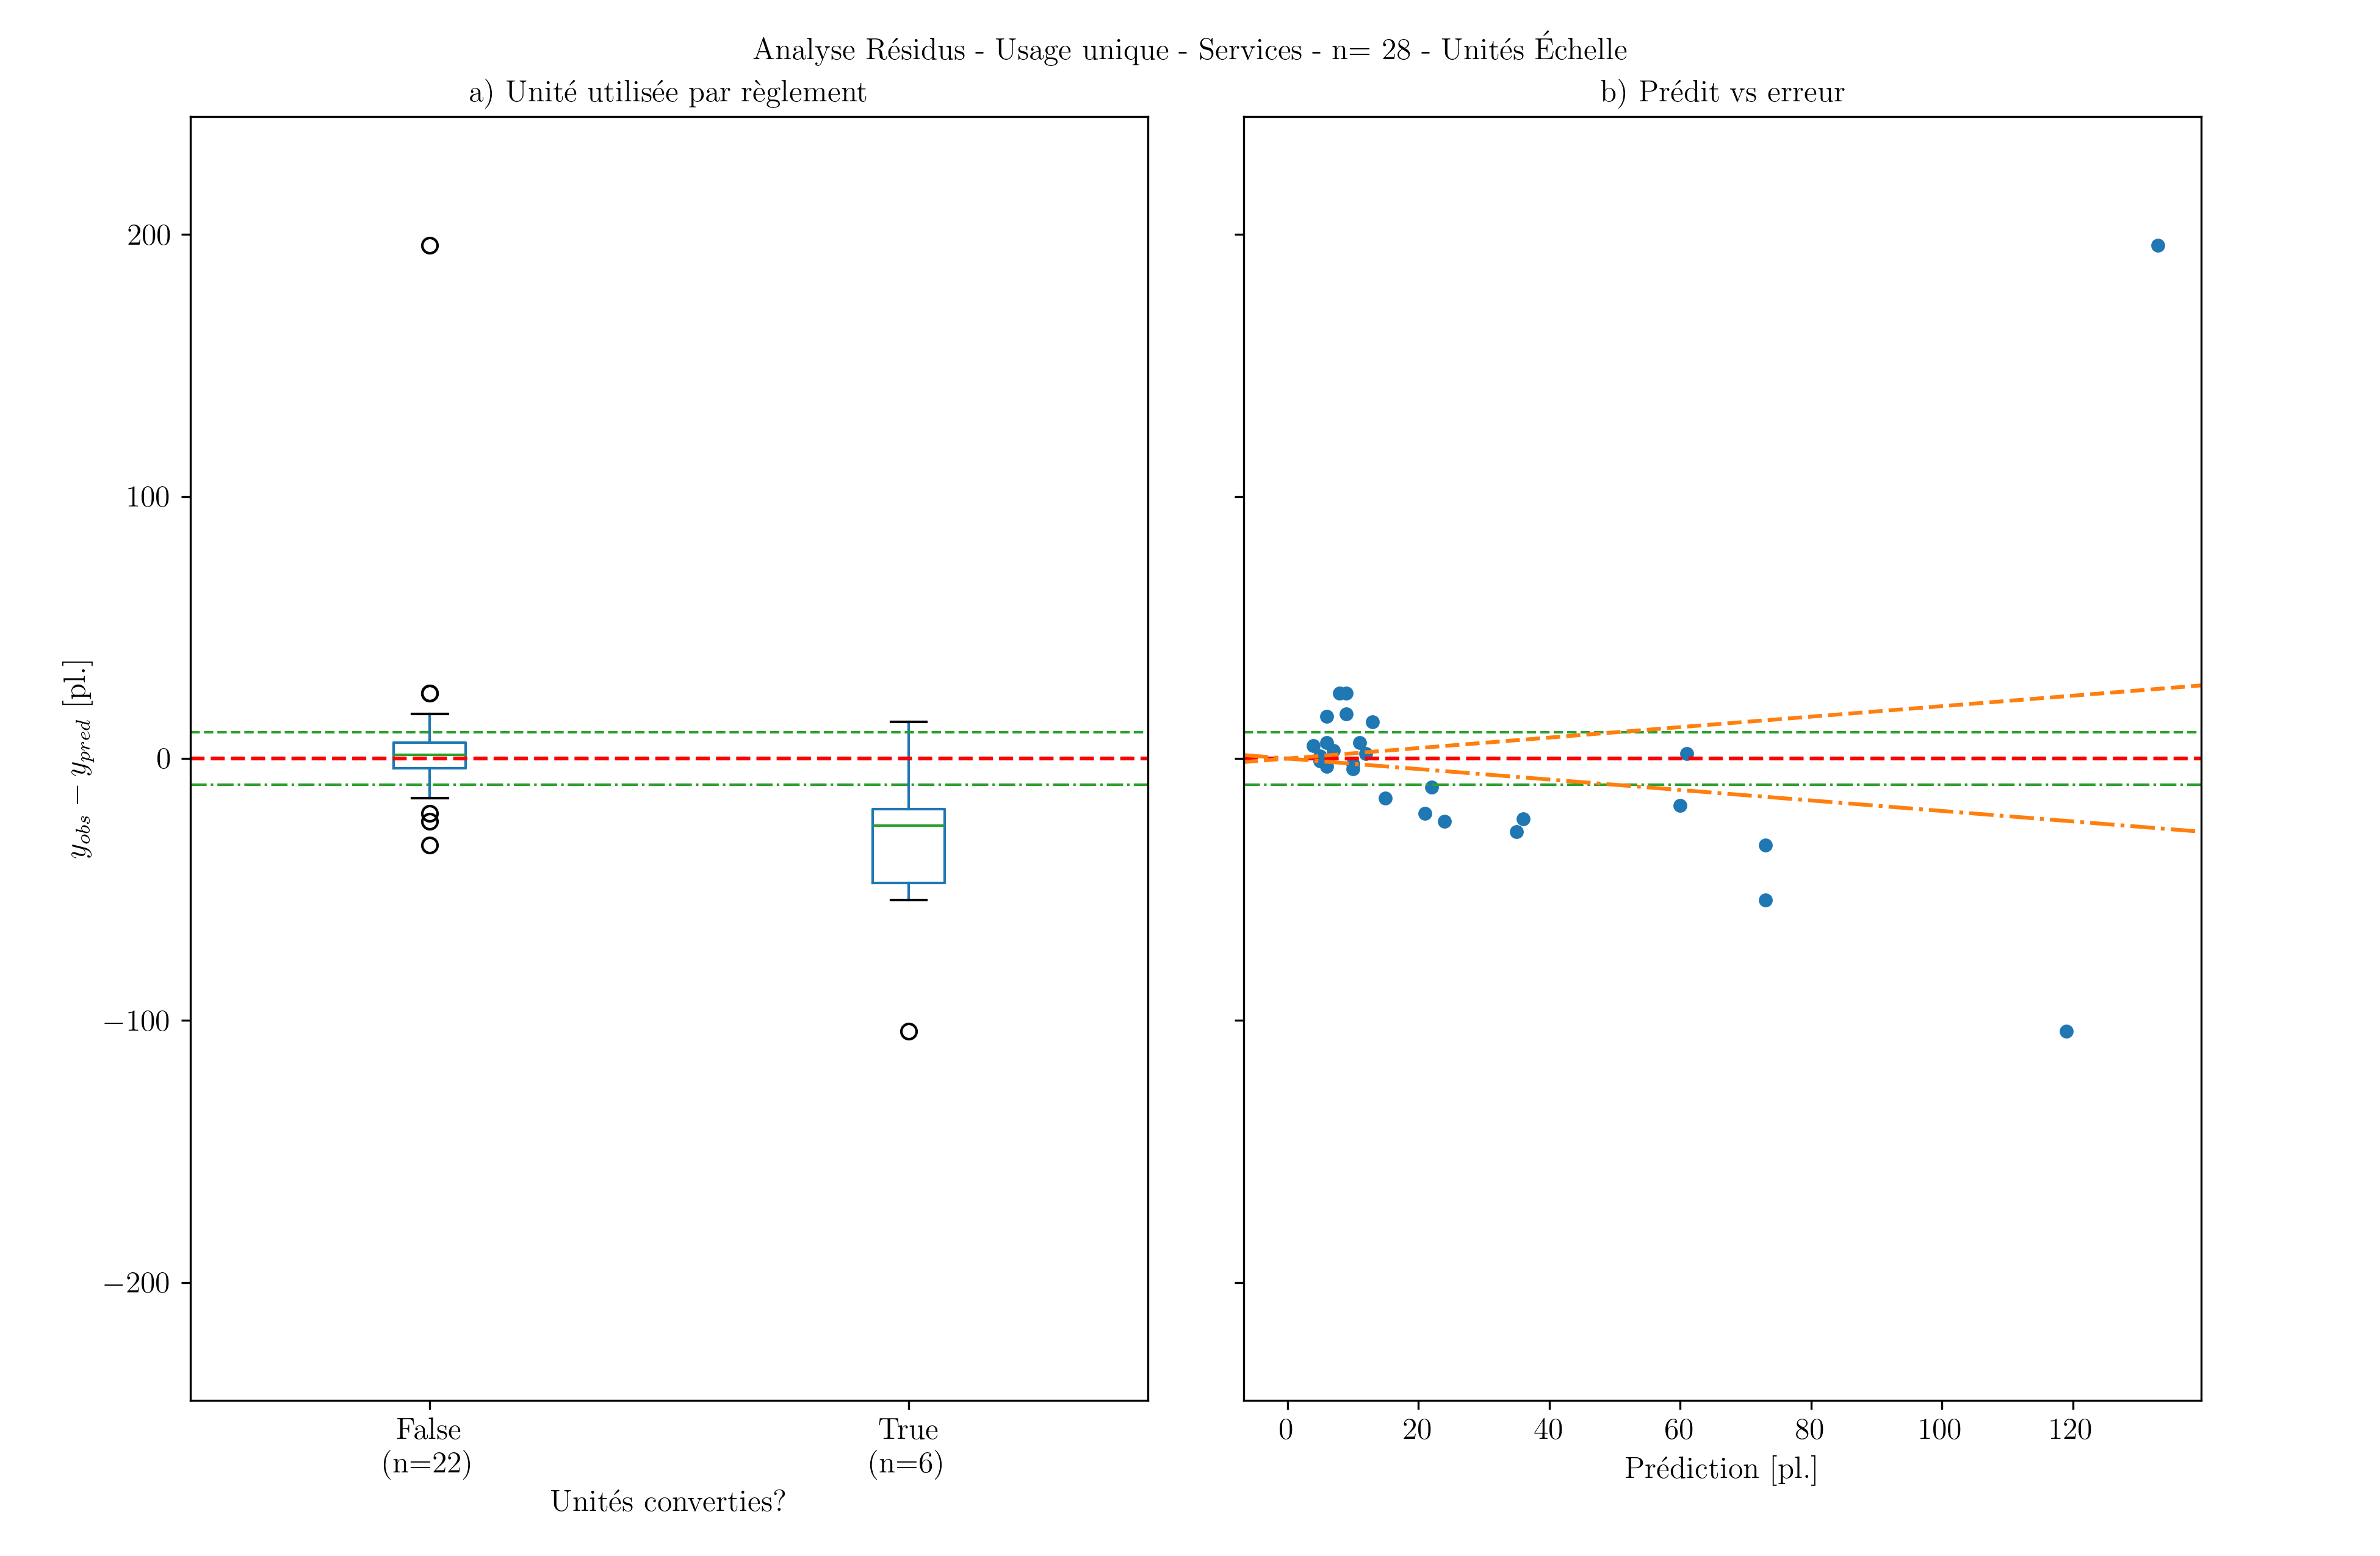
\includegraphics[width=1\linewidth]{images/ana_res_41_se_10_pe_20_c.png}
        \caption{Analyse des résidus en fonction de la prédiction et des unités de formulation pour les lots de services}
        \label{fig:ana-res-unit-pred-serv}
    \end{figure}
    \begin{figure}[H]
        \centering
        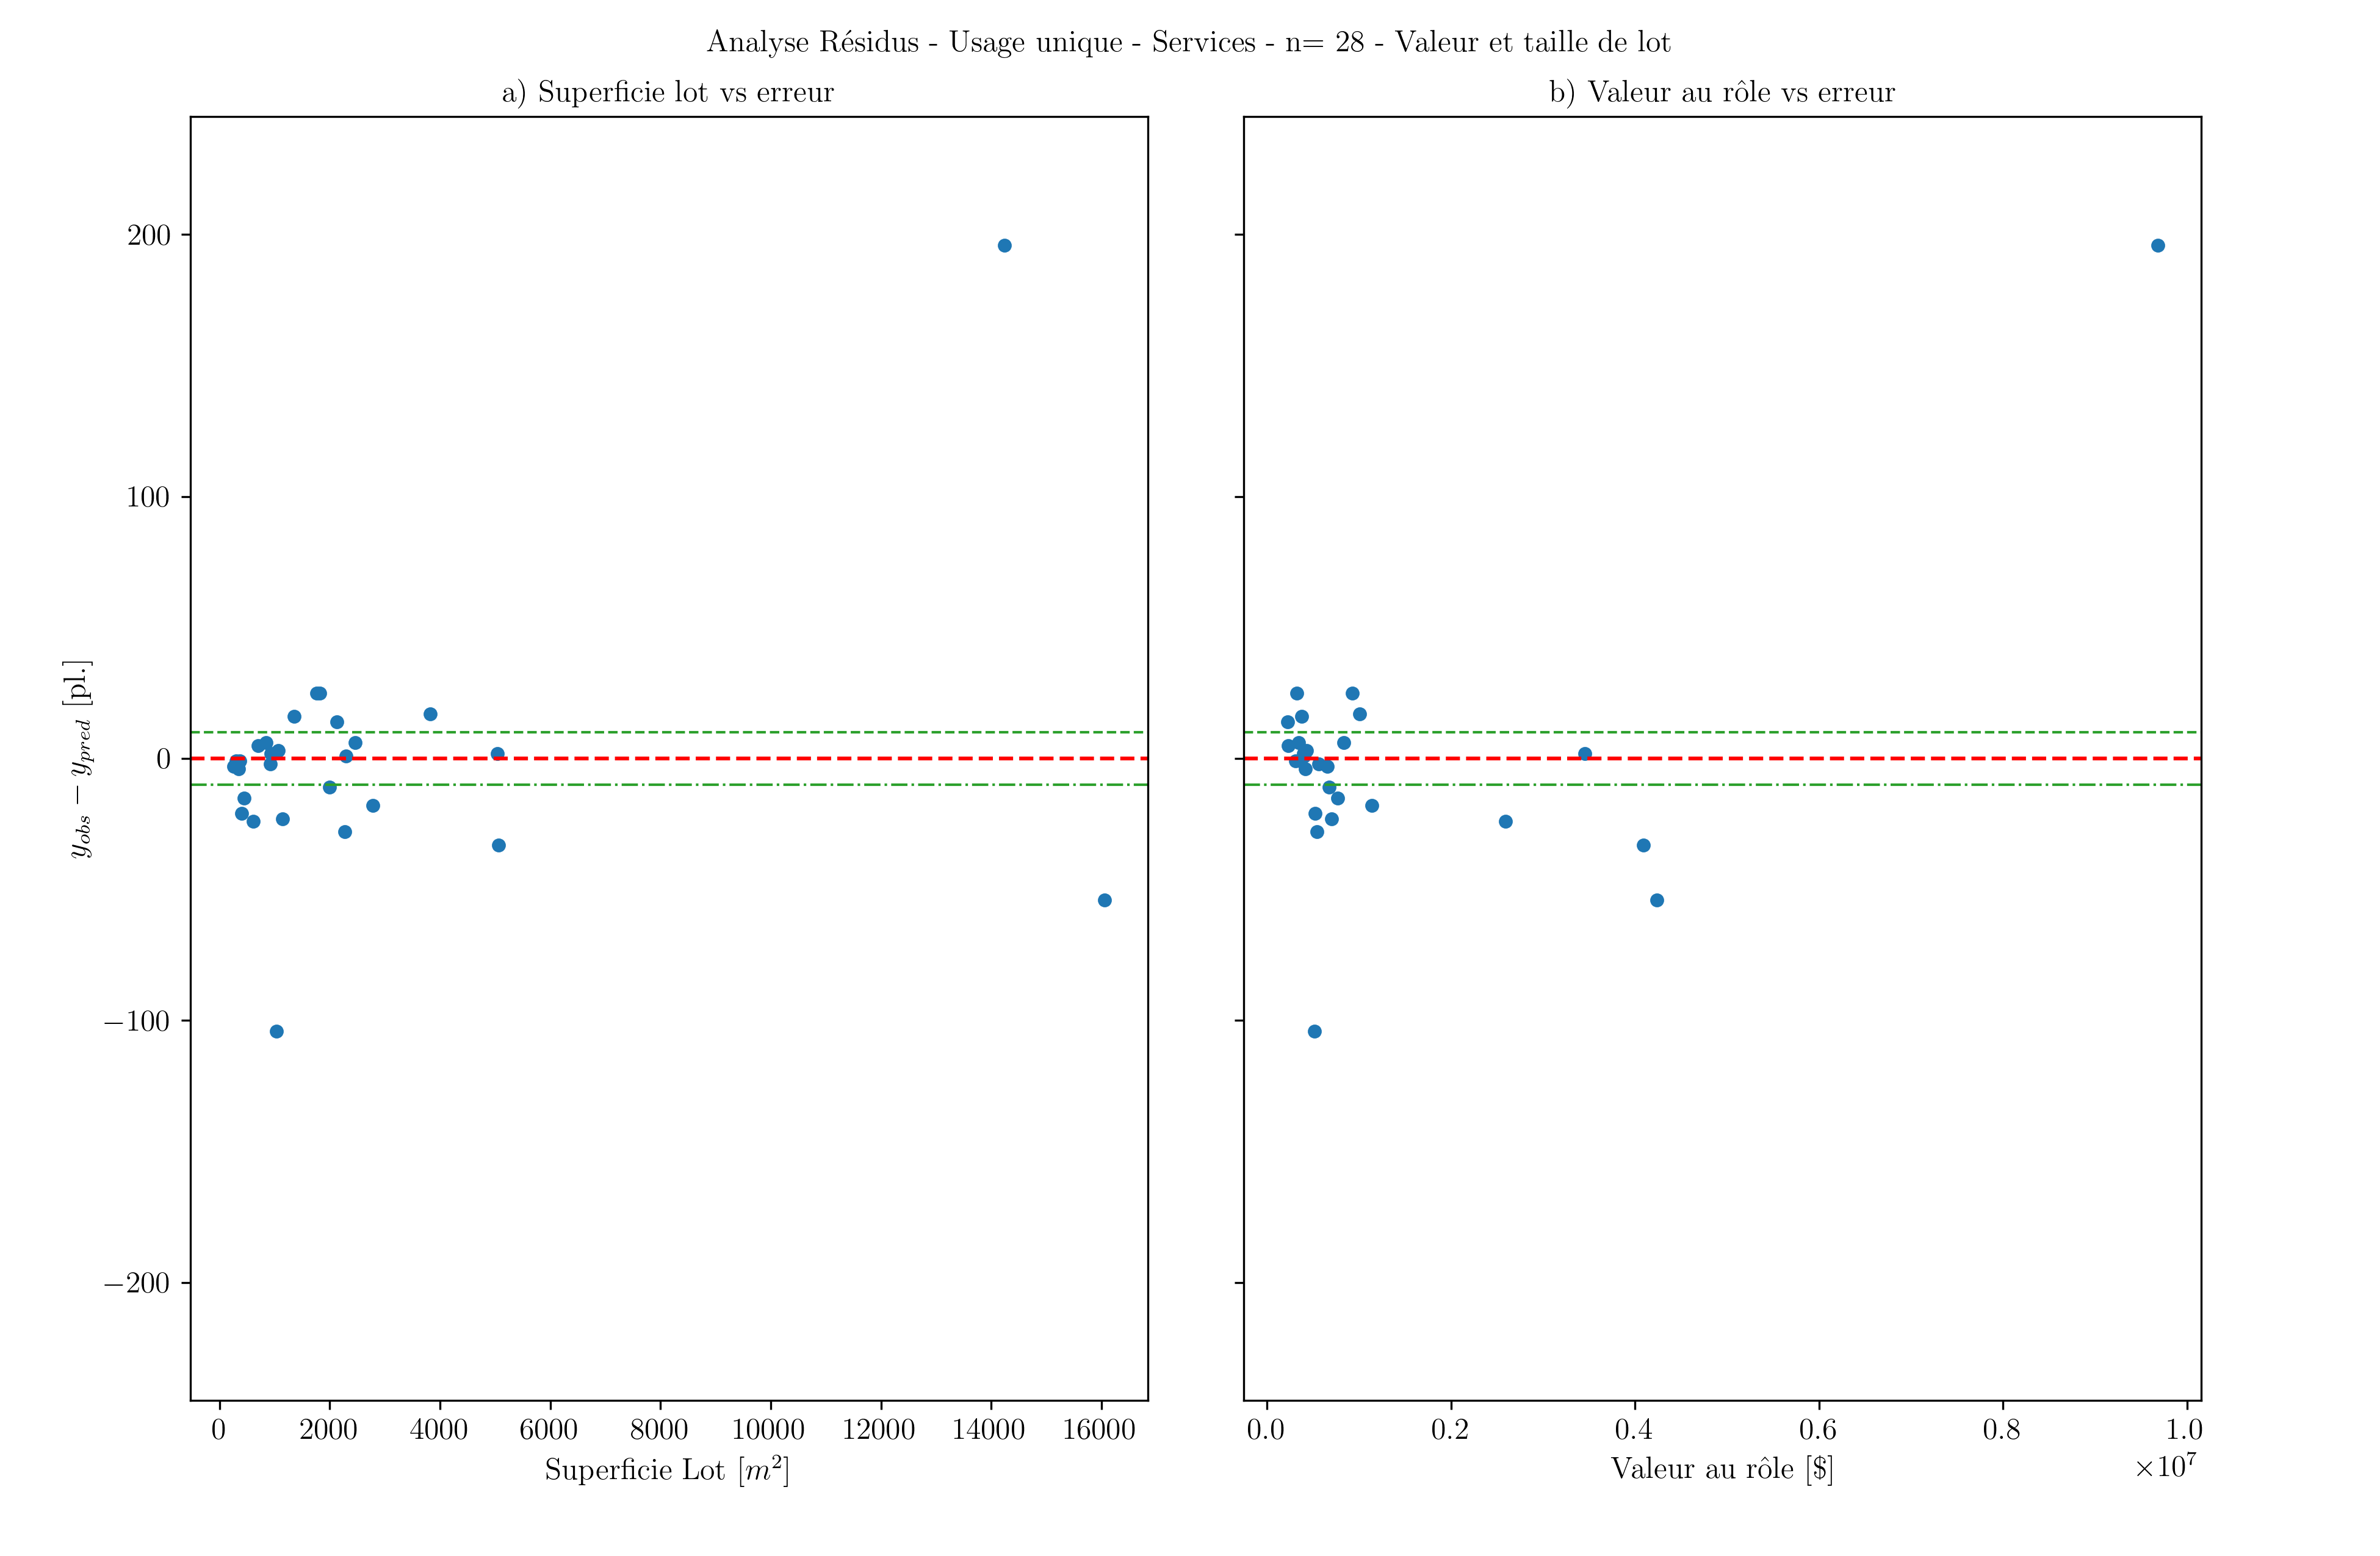
\includegraphics[width=1\linewidth]{images/ana_res_41_se_10_pe_20_d.png}
        \caption{Analyse des résidus en fonction de la superficie du lot et de la valeur pour les lots de services}
        \label{fig:ana-res-sup-val-serv}
    \end{figure}
    \begin{figure}[H]
        \centering
        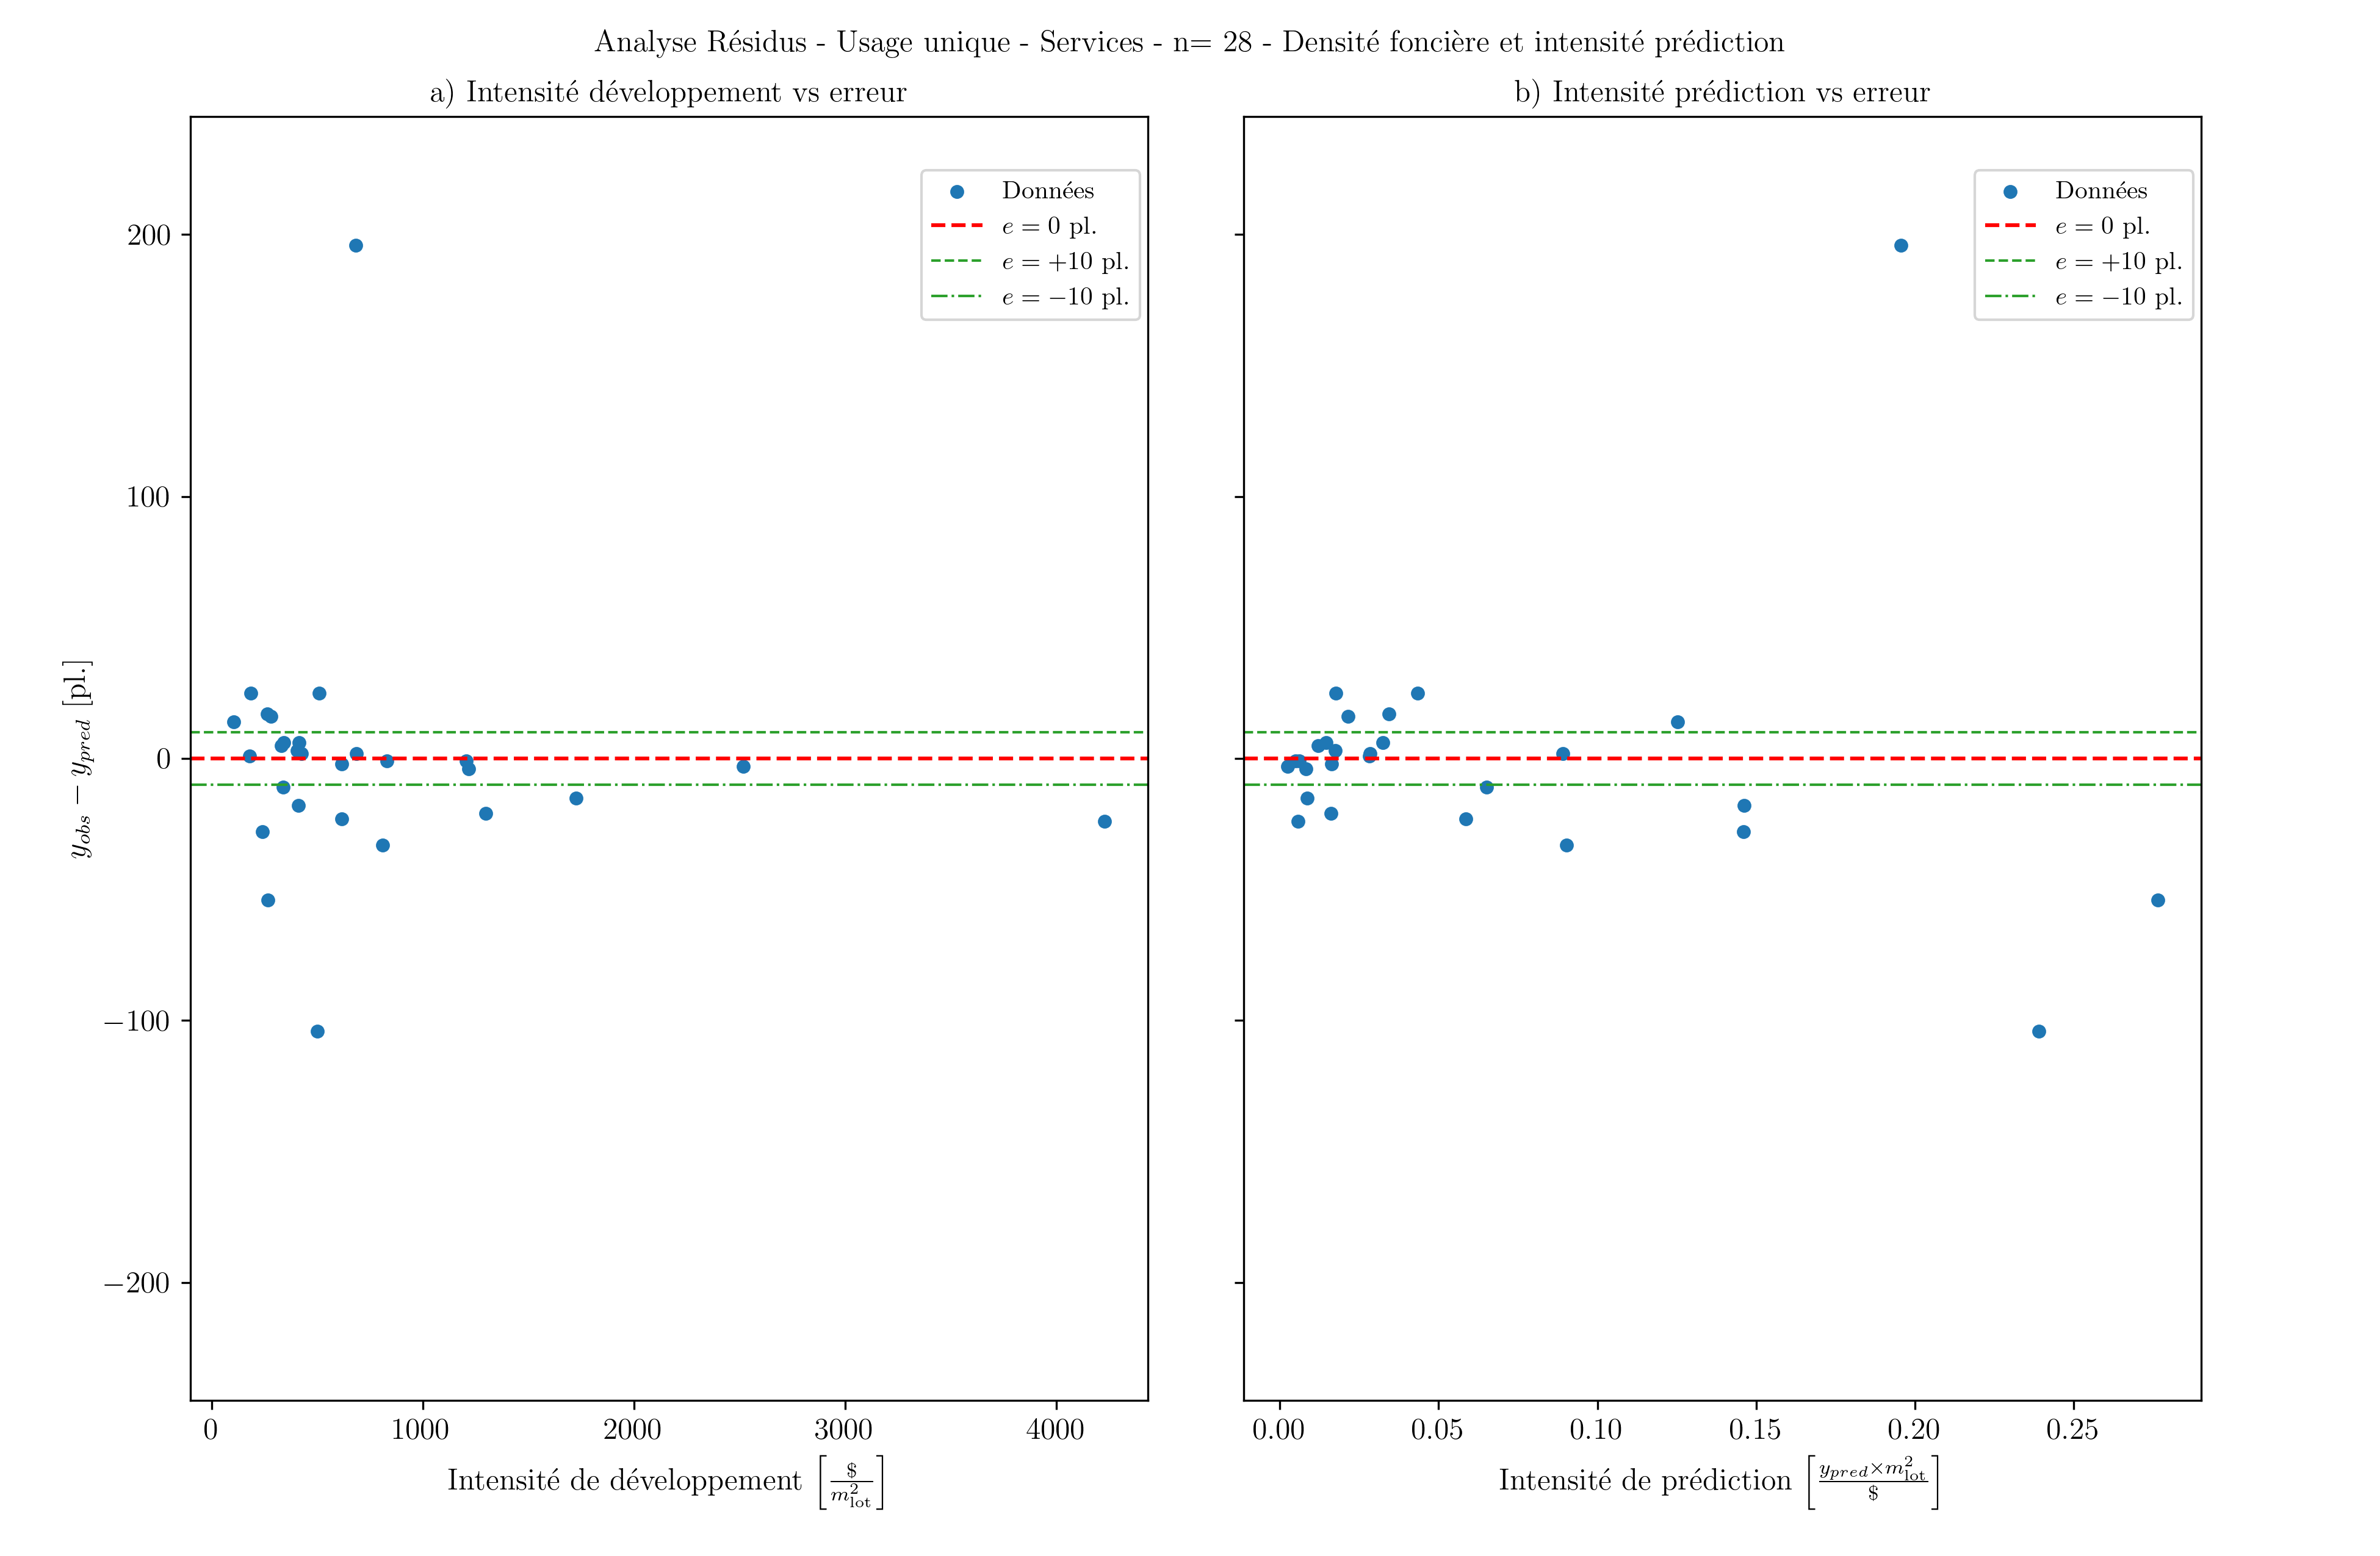
\includegraphics[width=1\linewidth]{images/ana_res_41_se_10_pe_20_e.png}
        \caption{Analyse des résidus en fonction de l'intensité de développement et l'intensité de prédiction pour les lots de services}
        \label{fig:ana-res-intens-serv}
    \end{figure}
\end{landscape}
\subsection{Industriel}
Vingt-sept lots industriels ont été échantillonnés. Une très grande usine ($a_l = 63000m^2$) avait une prédiction pour plus de 1170 places. Le règlement utilisé ici est formulé comme 1 place par employé ou 1 place par $95m^2$ au plus contraignant en combinaison avec le facteur de conversion fixé à 1 employé par $10m^2$ mène à cette surestimation. En utilisant seulement la formulation en mètres carrés, on obtient une prédiction de 124 places contre les 334 places constatées sur la propriété.\par
Contrairement aux autres catégories, le diagramme d'analyse des résidus sera présenté sans filtre et avec un filtre d'erreur maximale égal à 100 pour la rendre plus visible. Un filtre à une erreur de 75 places a été mis en place pour le calcul des métriques. Le modèle sous-estime systématiquement le nombre de places de stationnement après filtrage ($\bar{y}_{obs} = 26.76$ contre $\bar{y}_{pred} = 23.16$). \par
Le critère d'intensité de prédiction a de nouveau été utilisé à différents seuils pour trouver les lots qui ont potentiellement de fortes erreurs. À des niveaux de seuil de 0.05, 0.1 et 0.15, on trouve 25, 10 et 7 propriétés avec le potentiel d'avoir de fortes erreurs. Aucune tendance structurelle ne semble avoir de l'influence sur l'erreur des prédictions.\par
Comme pour les autres catégories, l'unité de formulation du règlement a un impact sur la précision des prédictions. La figure \ref{fig:ind-err-by-unit} montre l'erreur selon le type d'unité utilisée dans la formulation du règlement et on constate encore que les conversions d'unité sont une importante source d'erreur.

\begin{landscape}
    \begin{figure}[H]
        \centering
        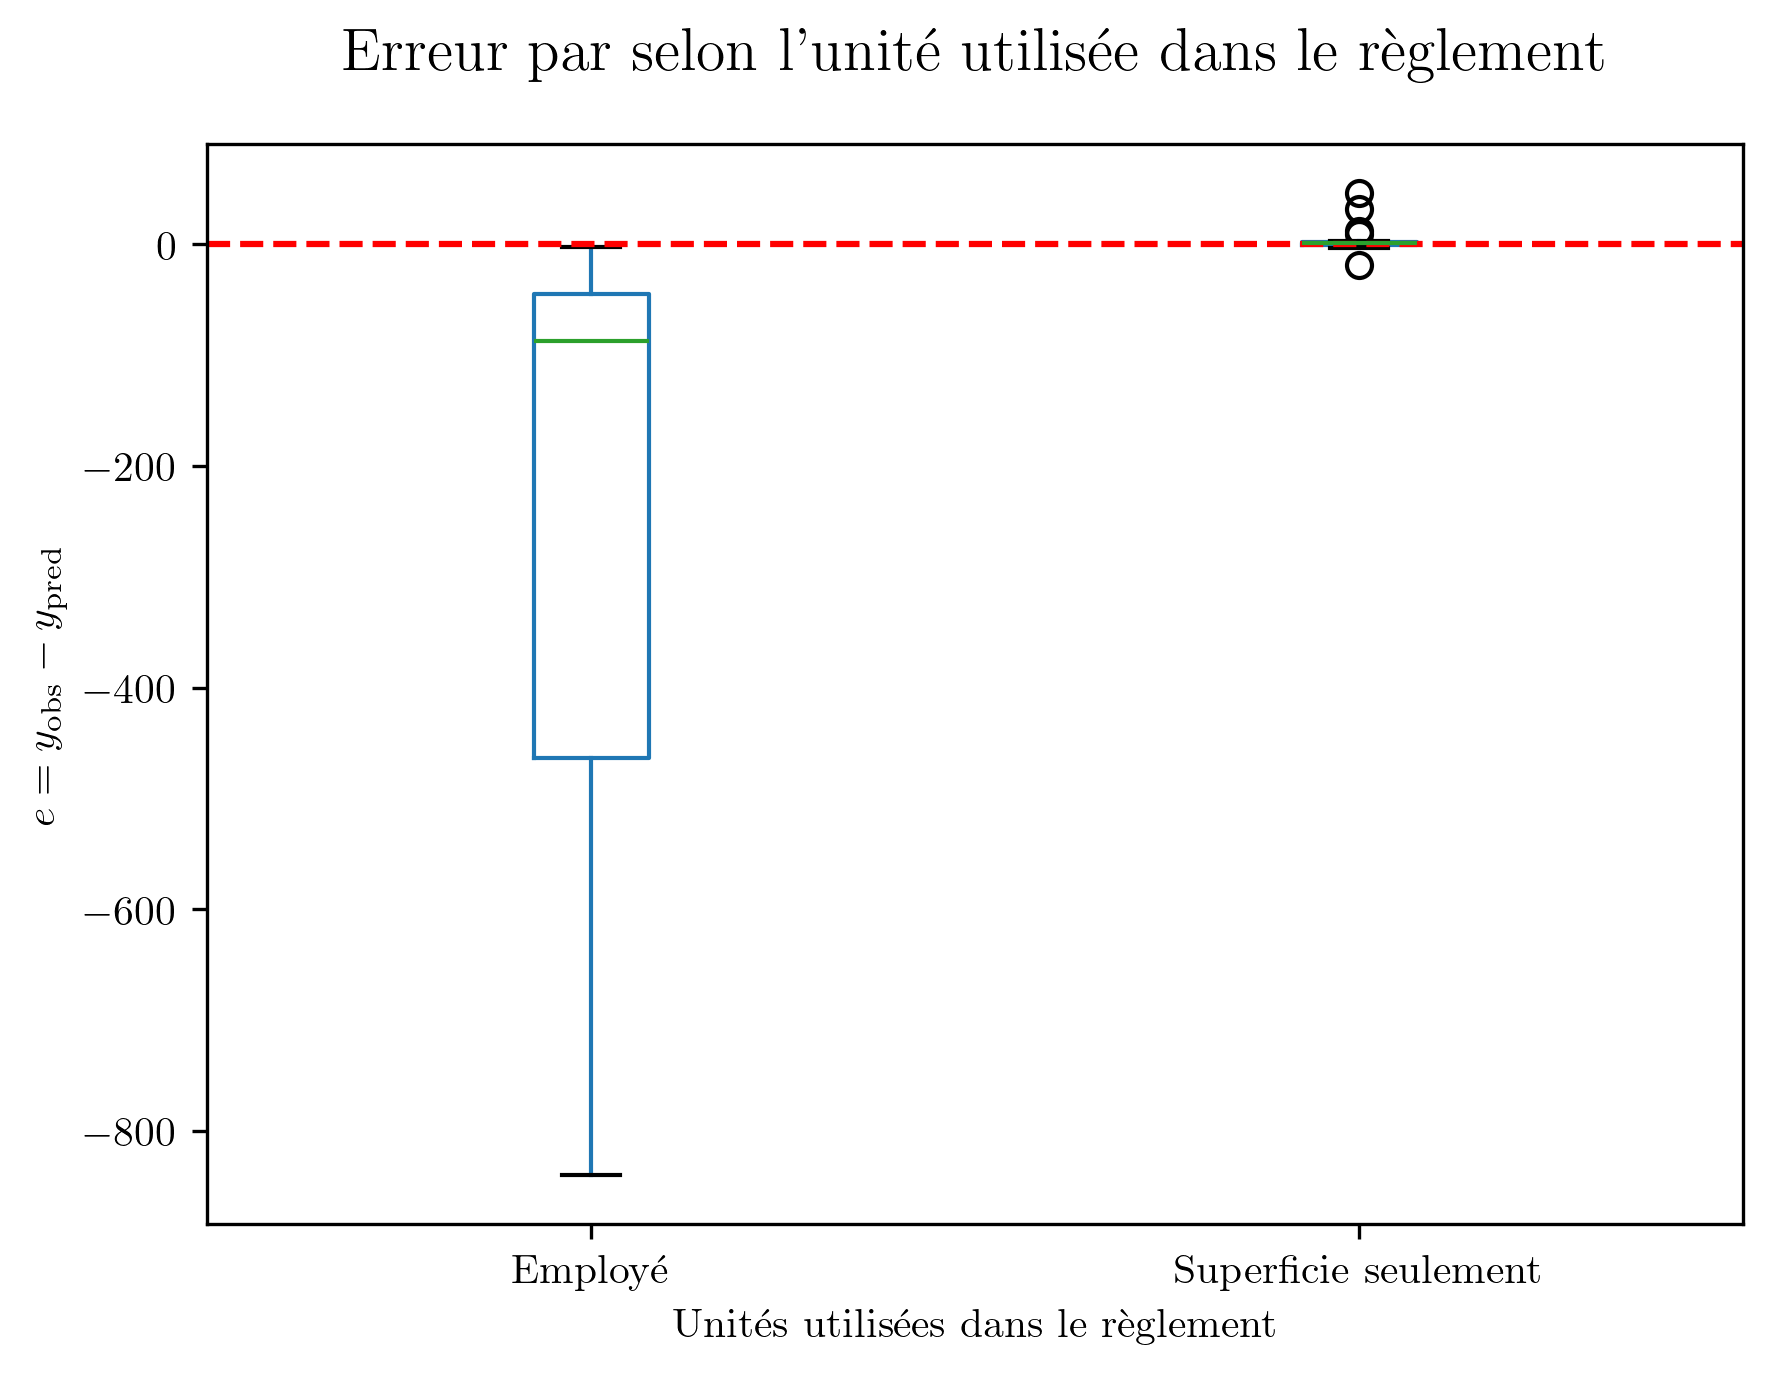
\includegraphics[width=0.7\linewidth]{images/boxplot_error_by_category_39.png}
        \caption{Diagramme à boîte de l'erreur en fonction de l'unité de formulation du règlement pour l'industrie}
        \label{fig:ind-err-by-unit}
    \end{figure}
    %\begin{figure}[H]
    %    \centering
    %    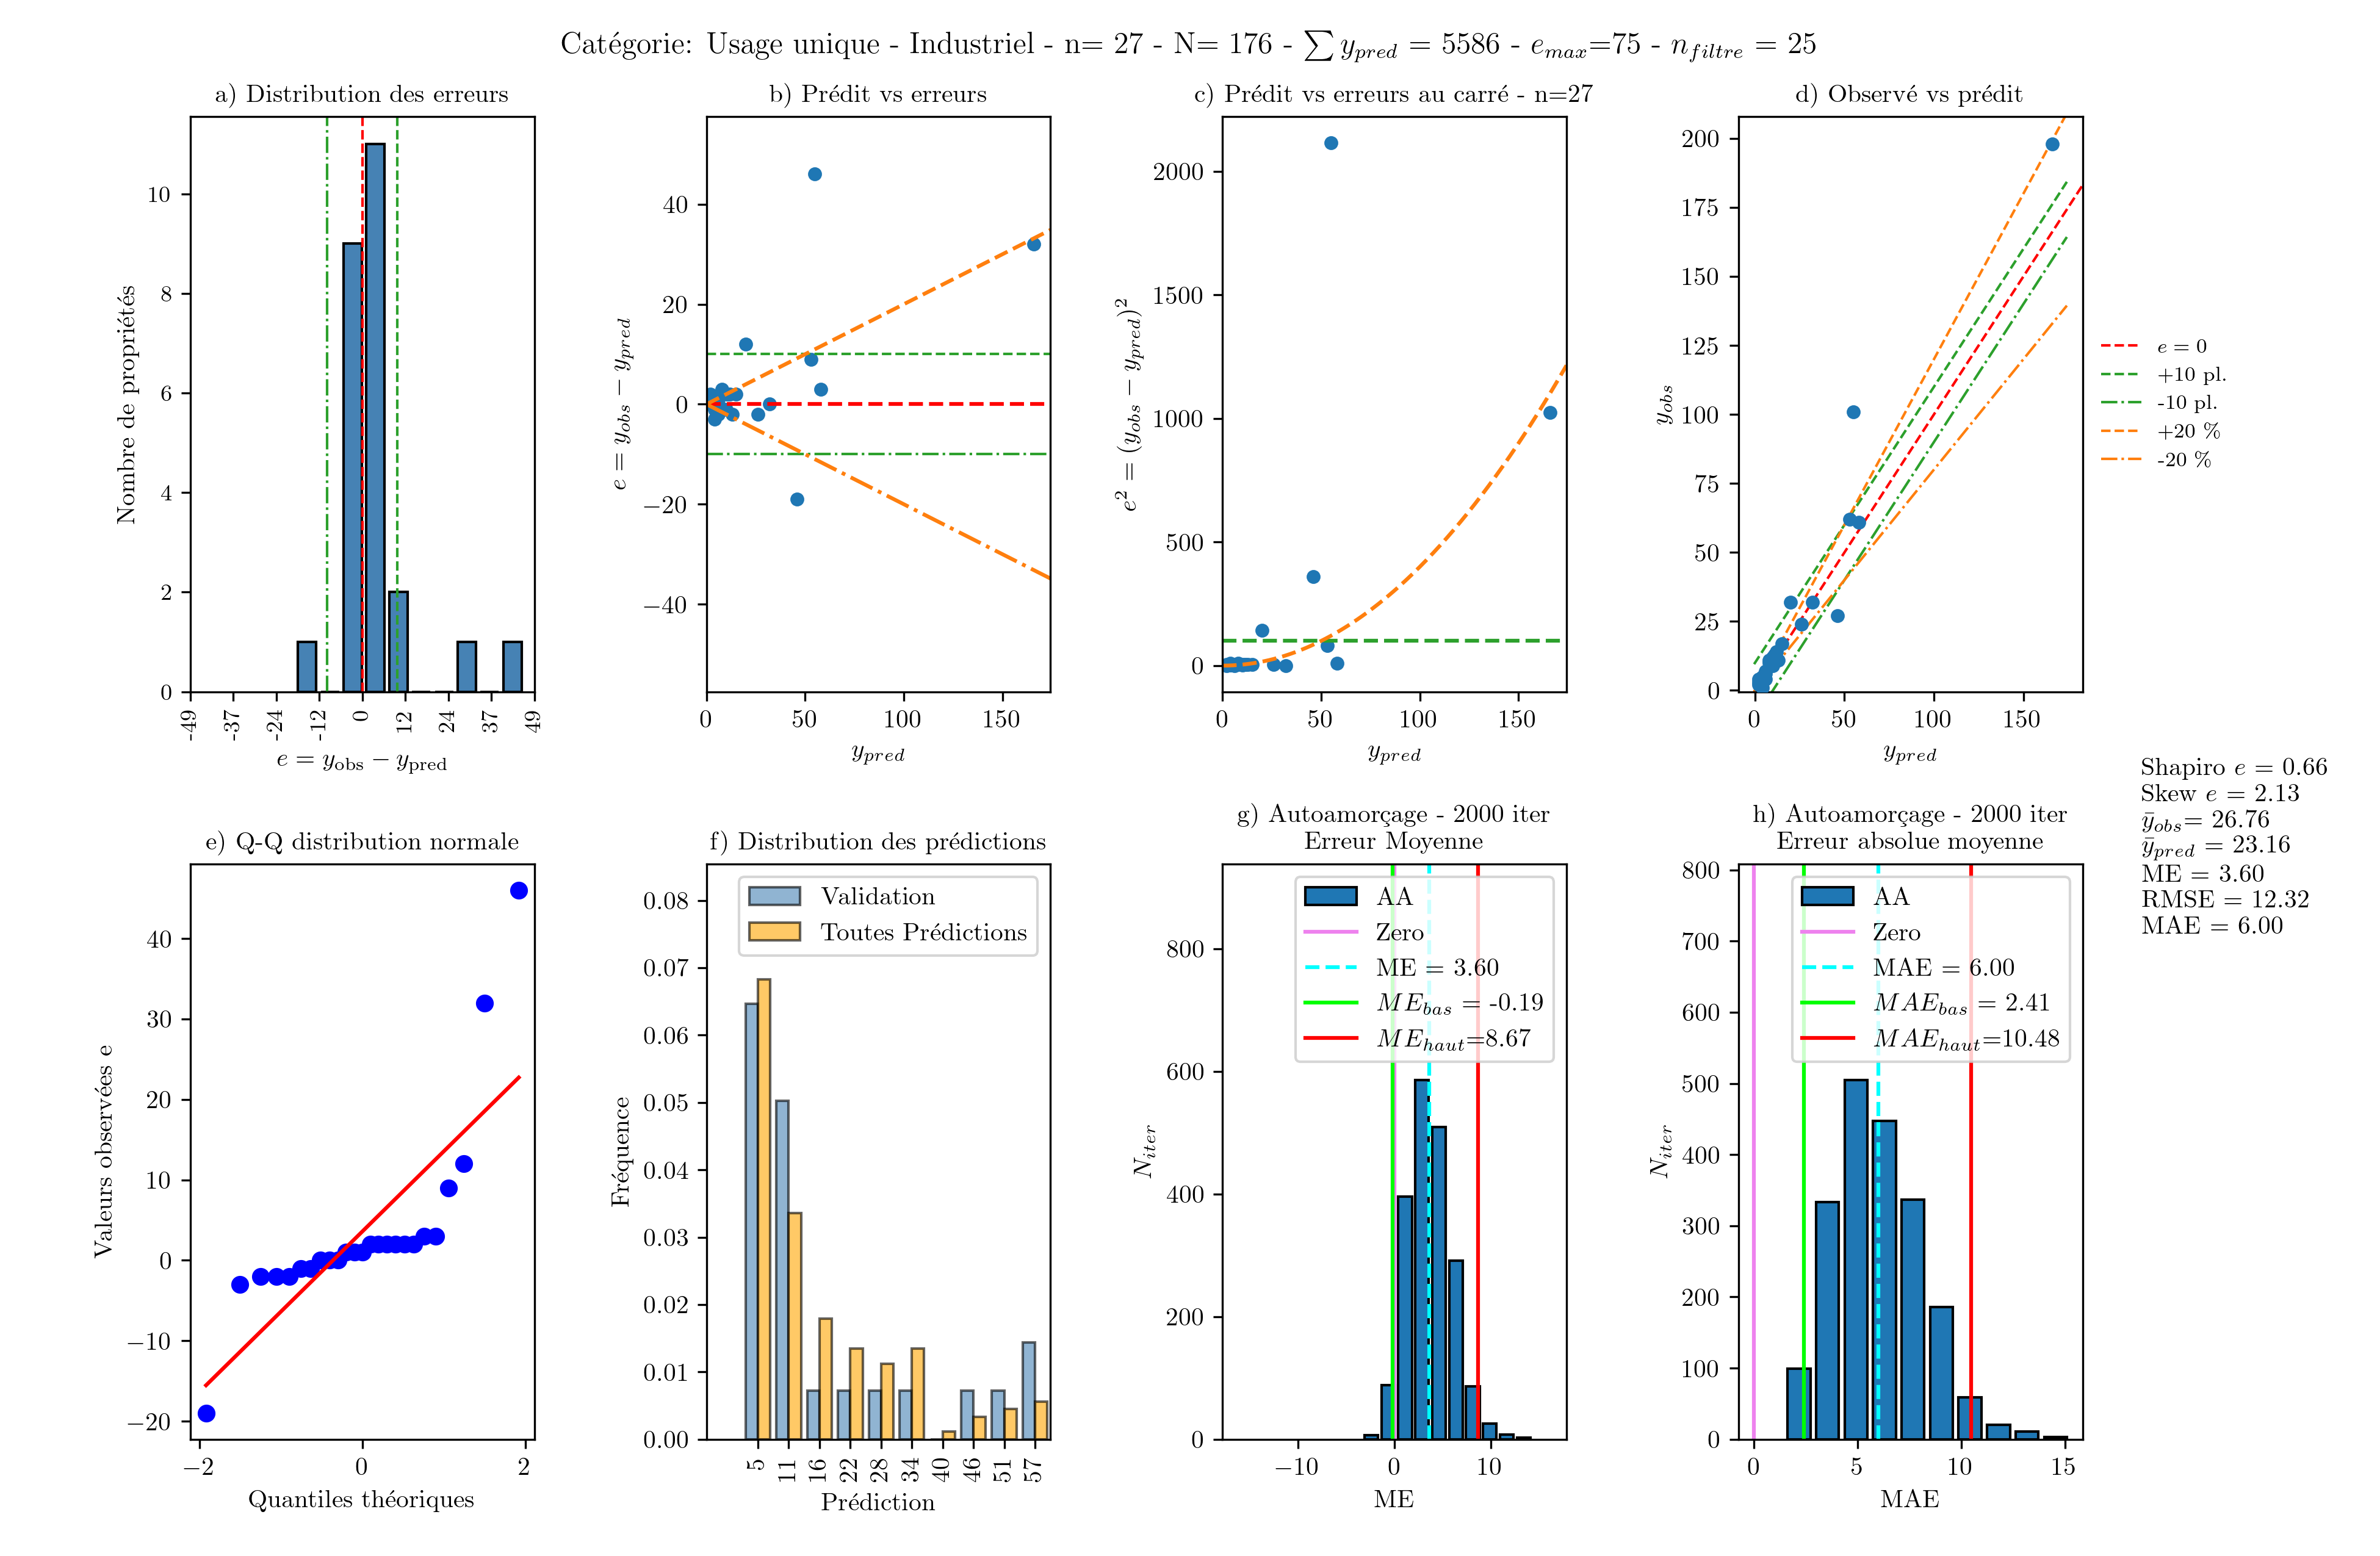
\includegraphics[scale=0.65]{images/int_erreur_39_e_75_se_10_pe_20.png}
    %    \label{fig:intervals-dis-val-serv-e100}
    %\end{figure}
    \begin{figure}[H]
        \centering
        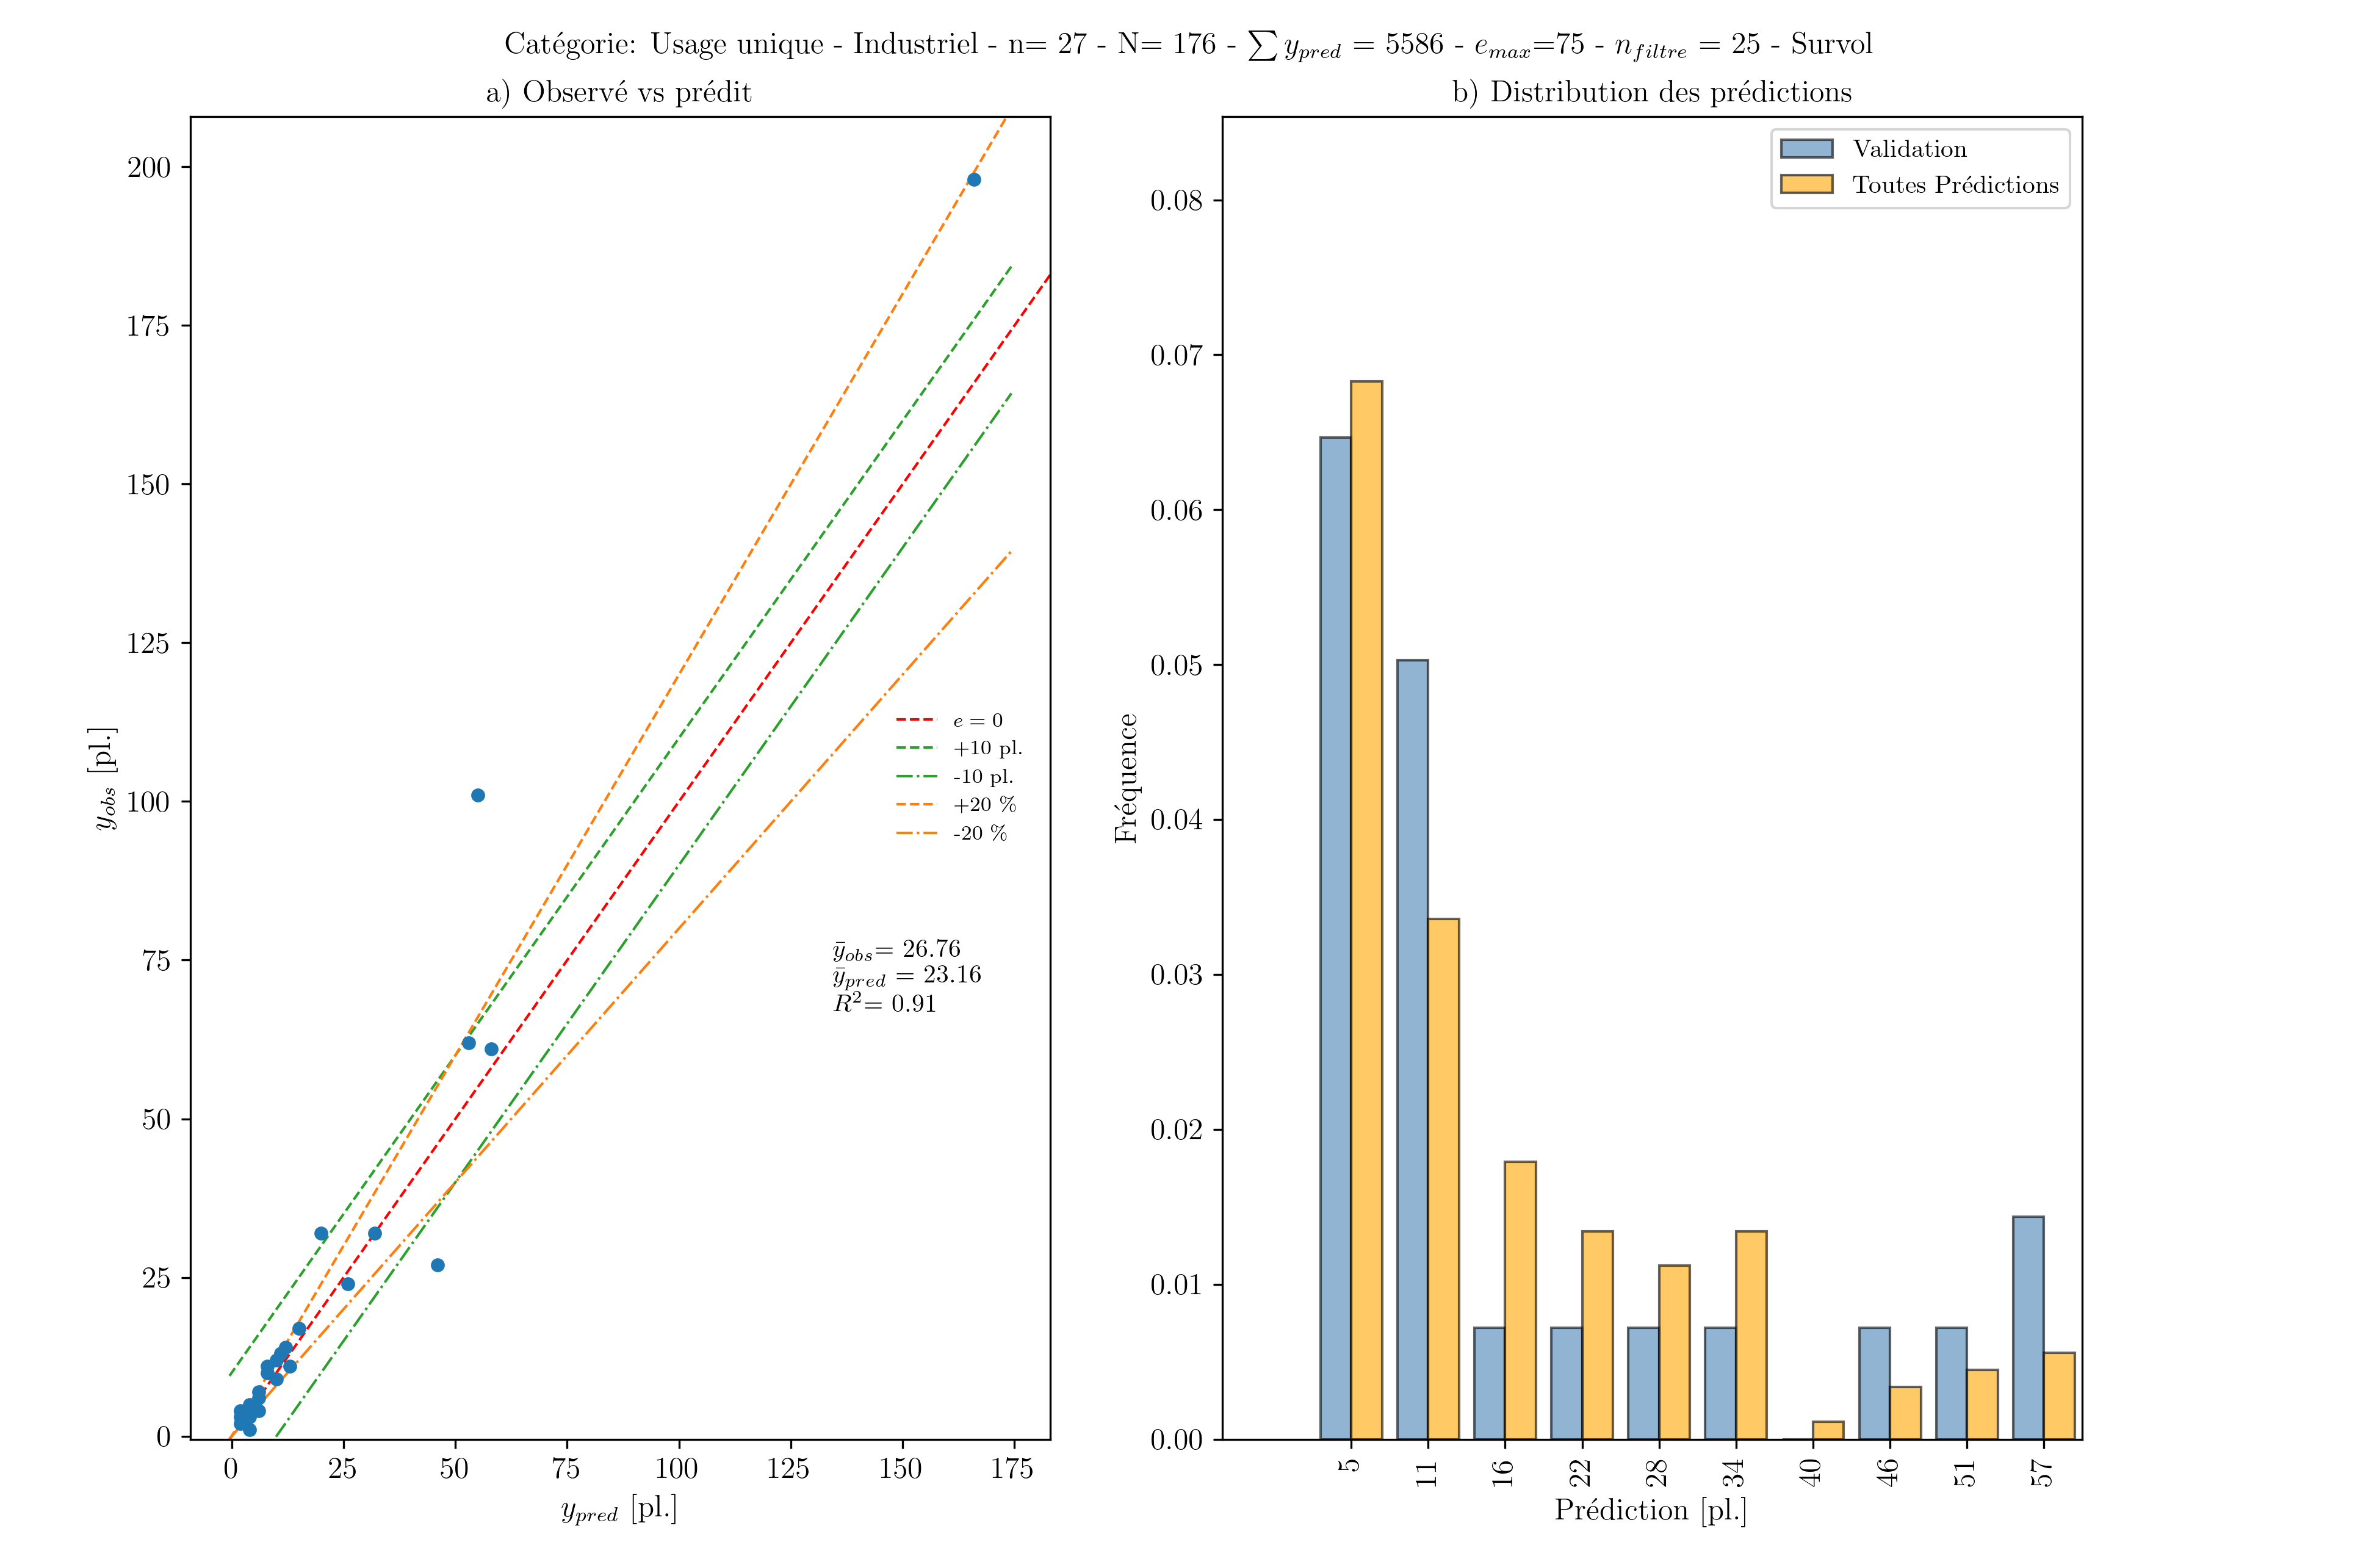
\includegraphics[width=1\linewidth]{images/int_erreur_39_e_75_se_10_pe_20_a.png}
        \caption{Distribution des prédictions pour les lots industriels}
        \label{fig:int-dist-pred-ind}
    \end{figure}
    \begin{figure}[H]
        \centering
        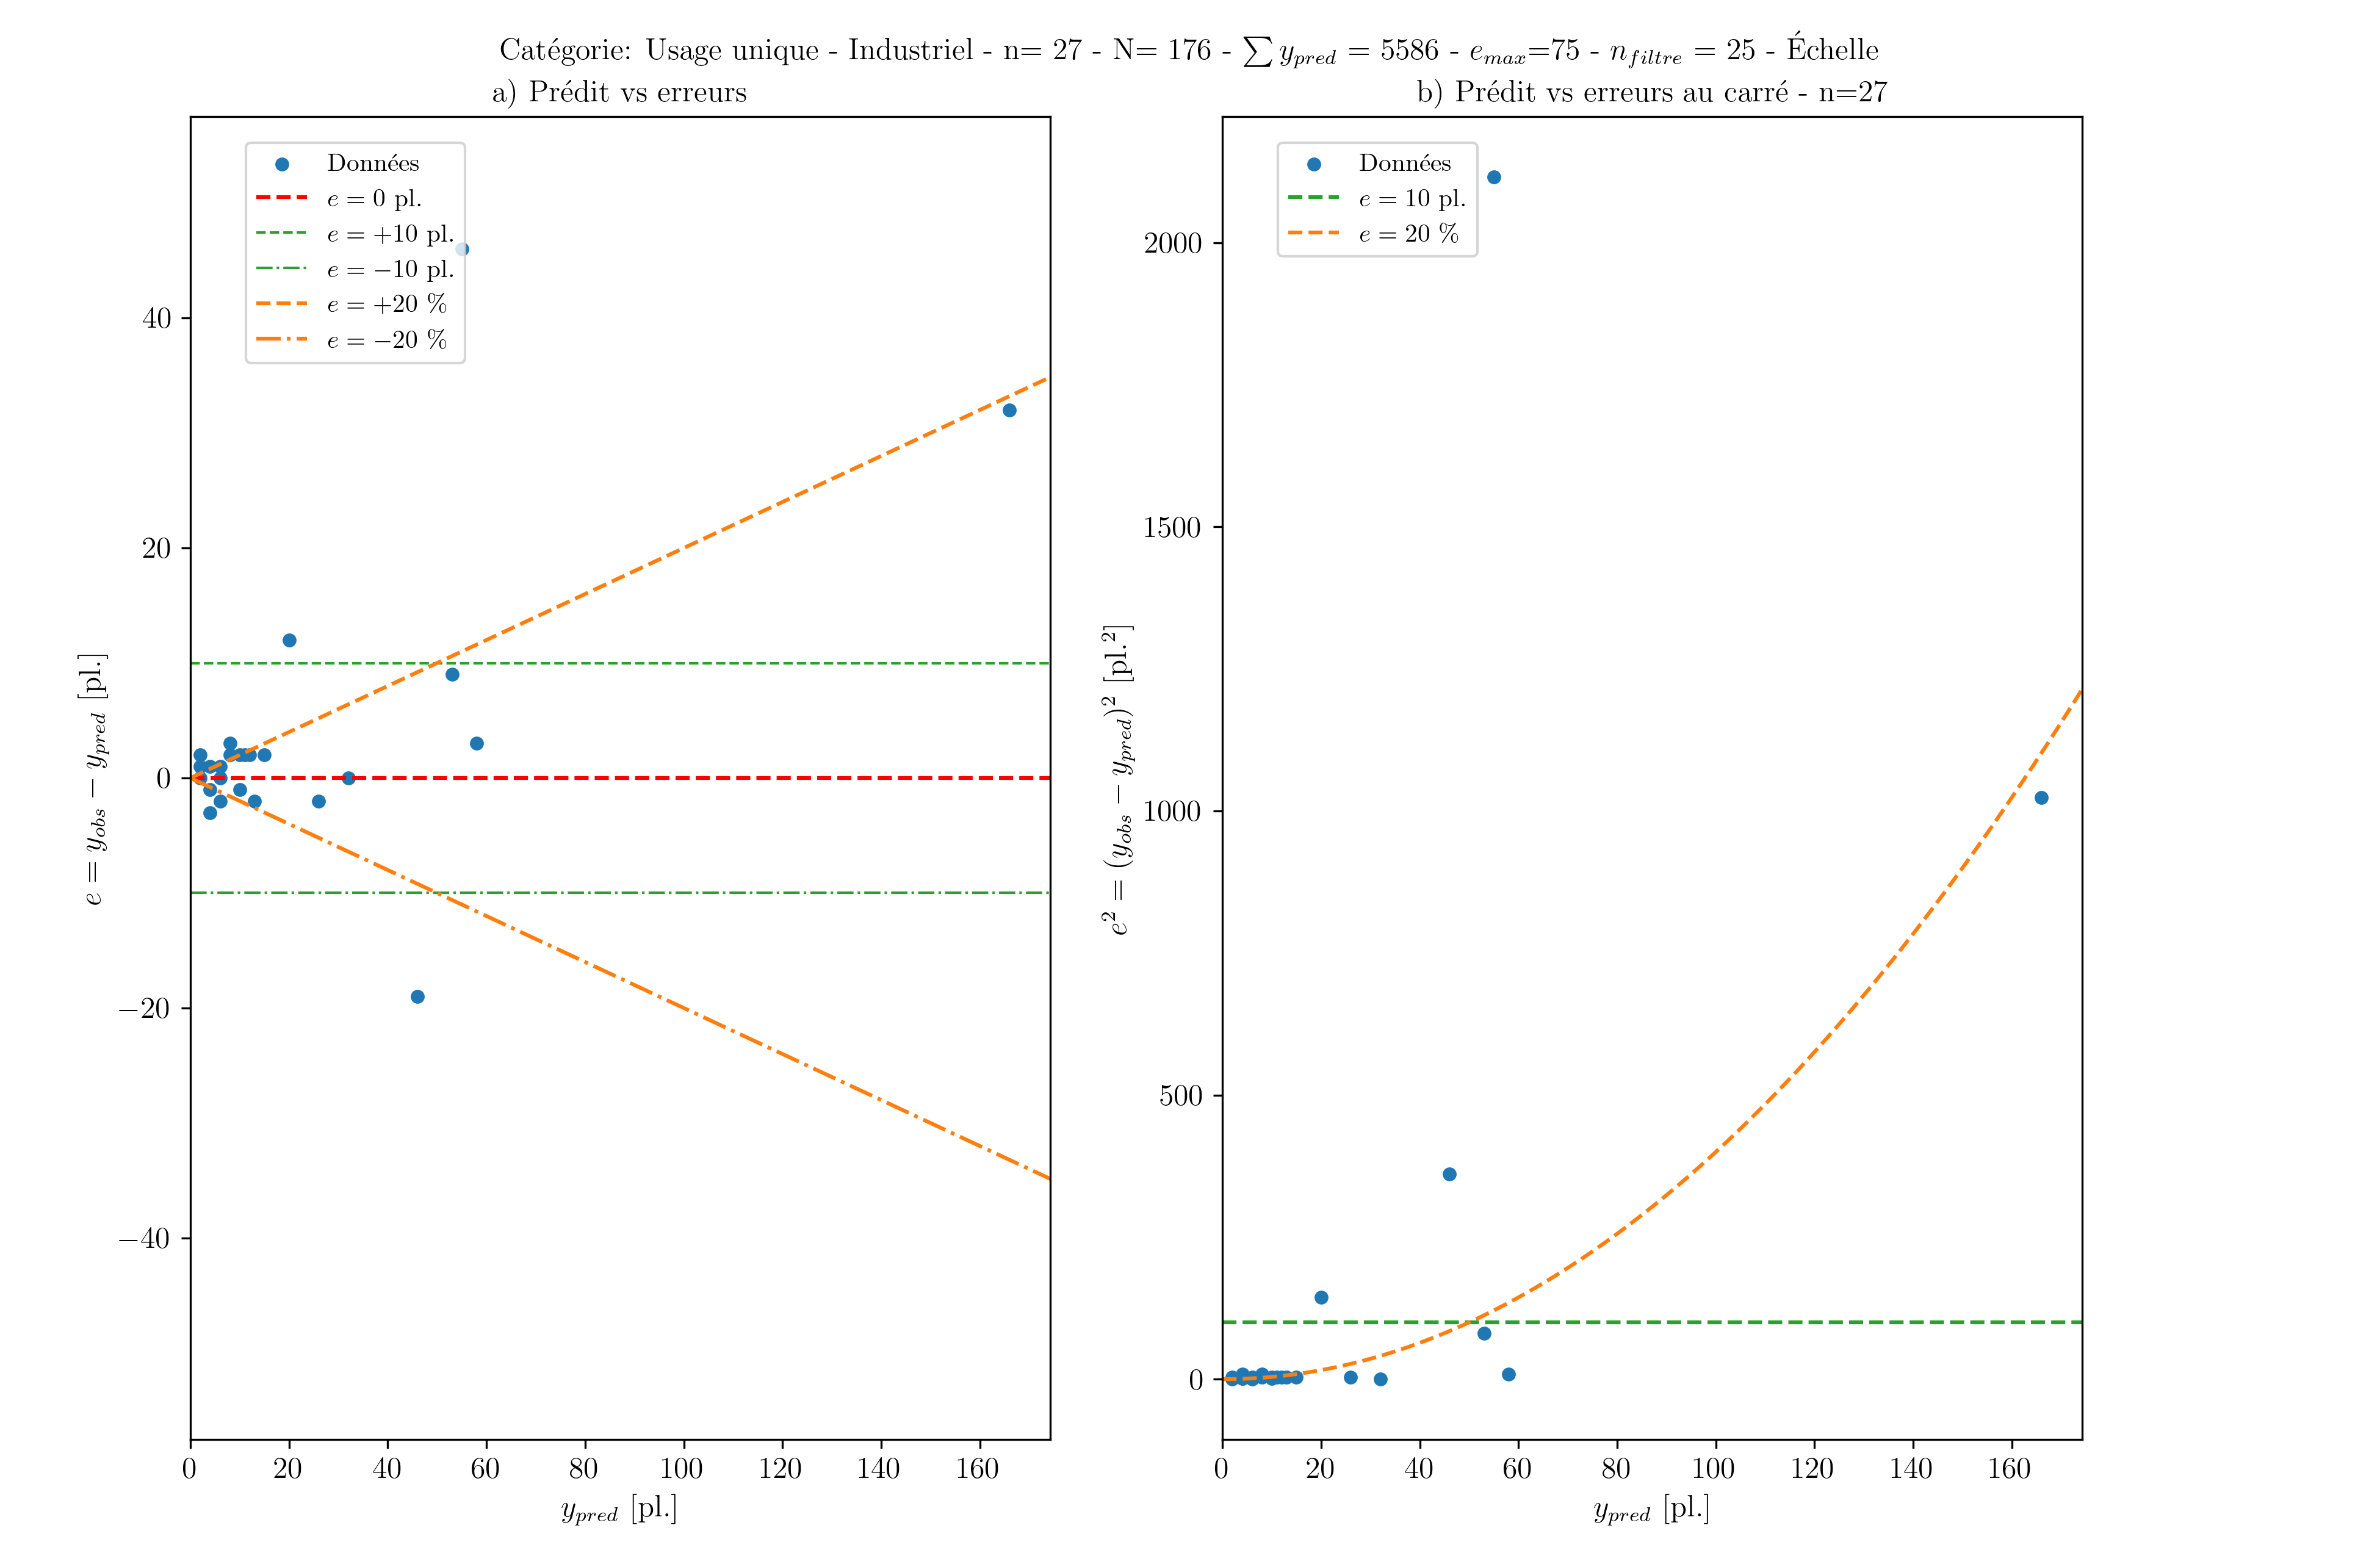
\includegraphics[width=1\linewidth]{images/int_erreur_39_e_75_se_10_pe_20_b.png}
        \caption{Erreur en fonction des prédictions pour les lots industriels}
        \label{fig:err-err-quad-pred-ind}
    \end{figure}
    \begin{figure}[H]
        \centering
        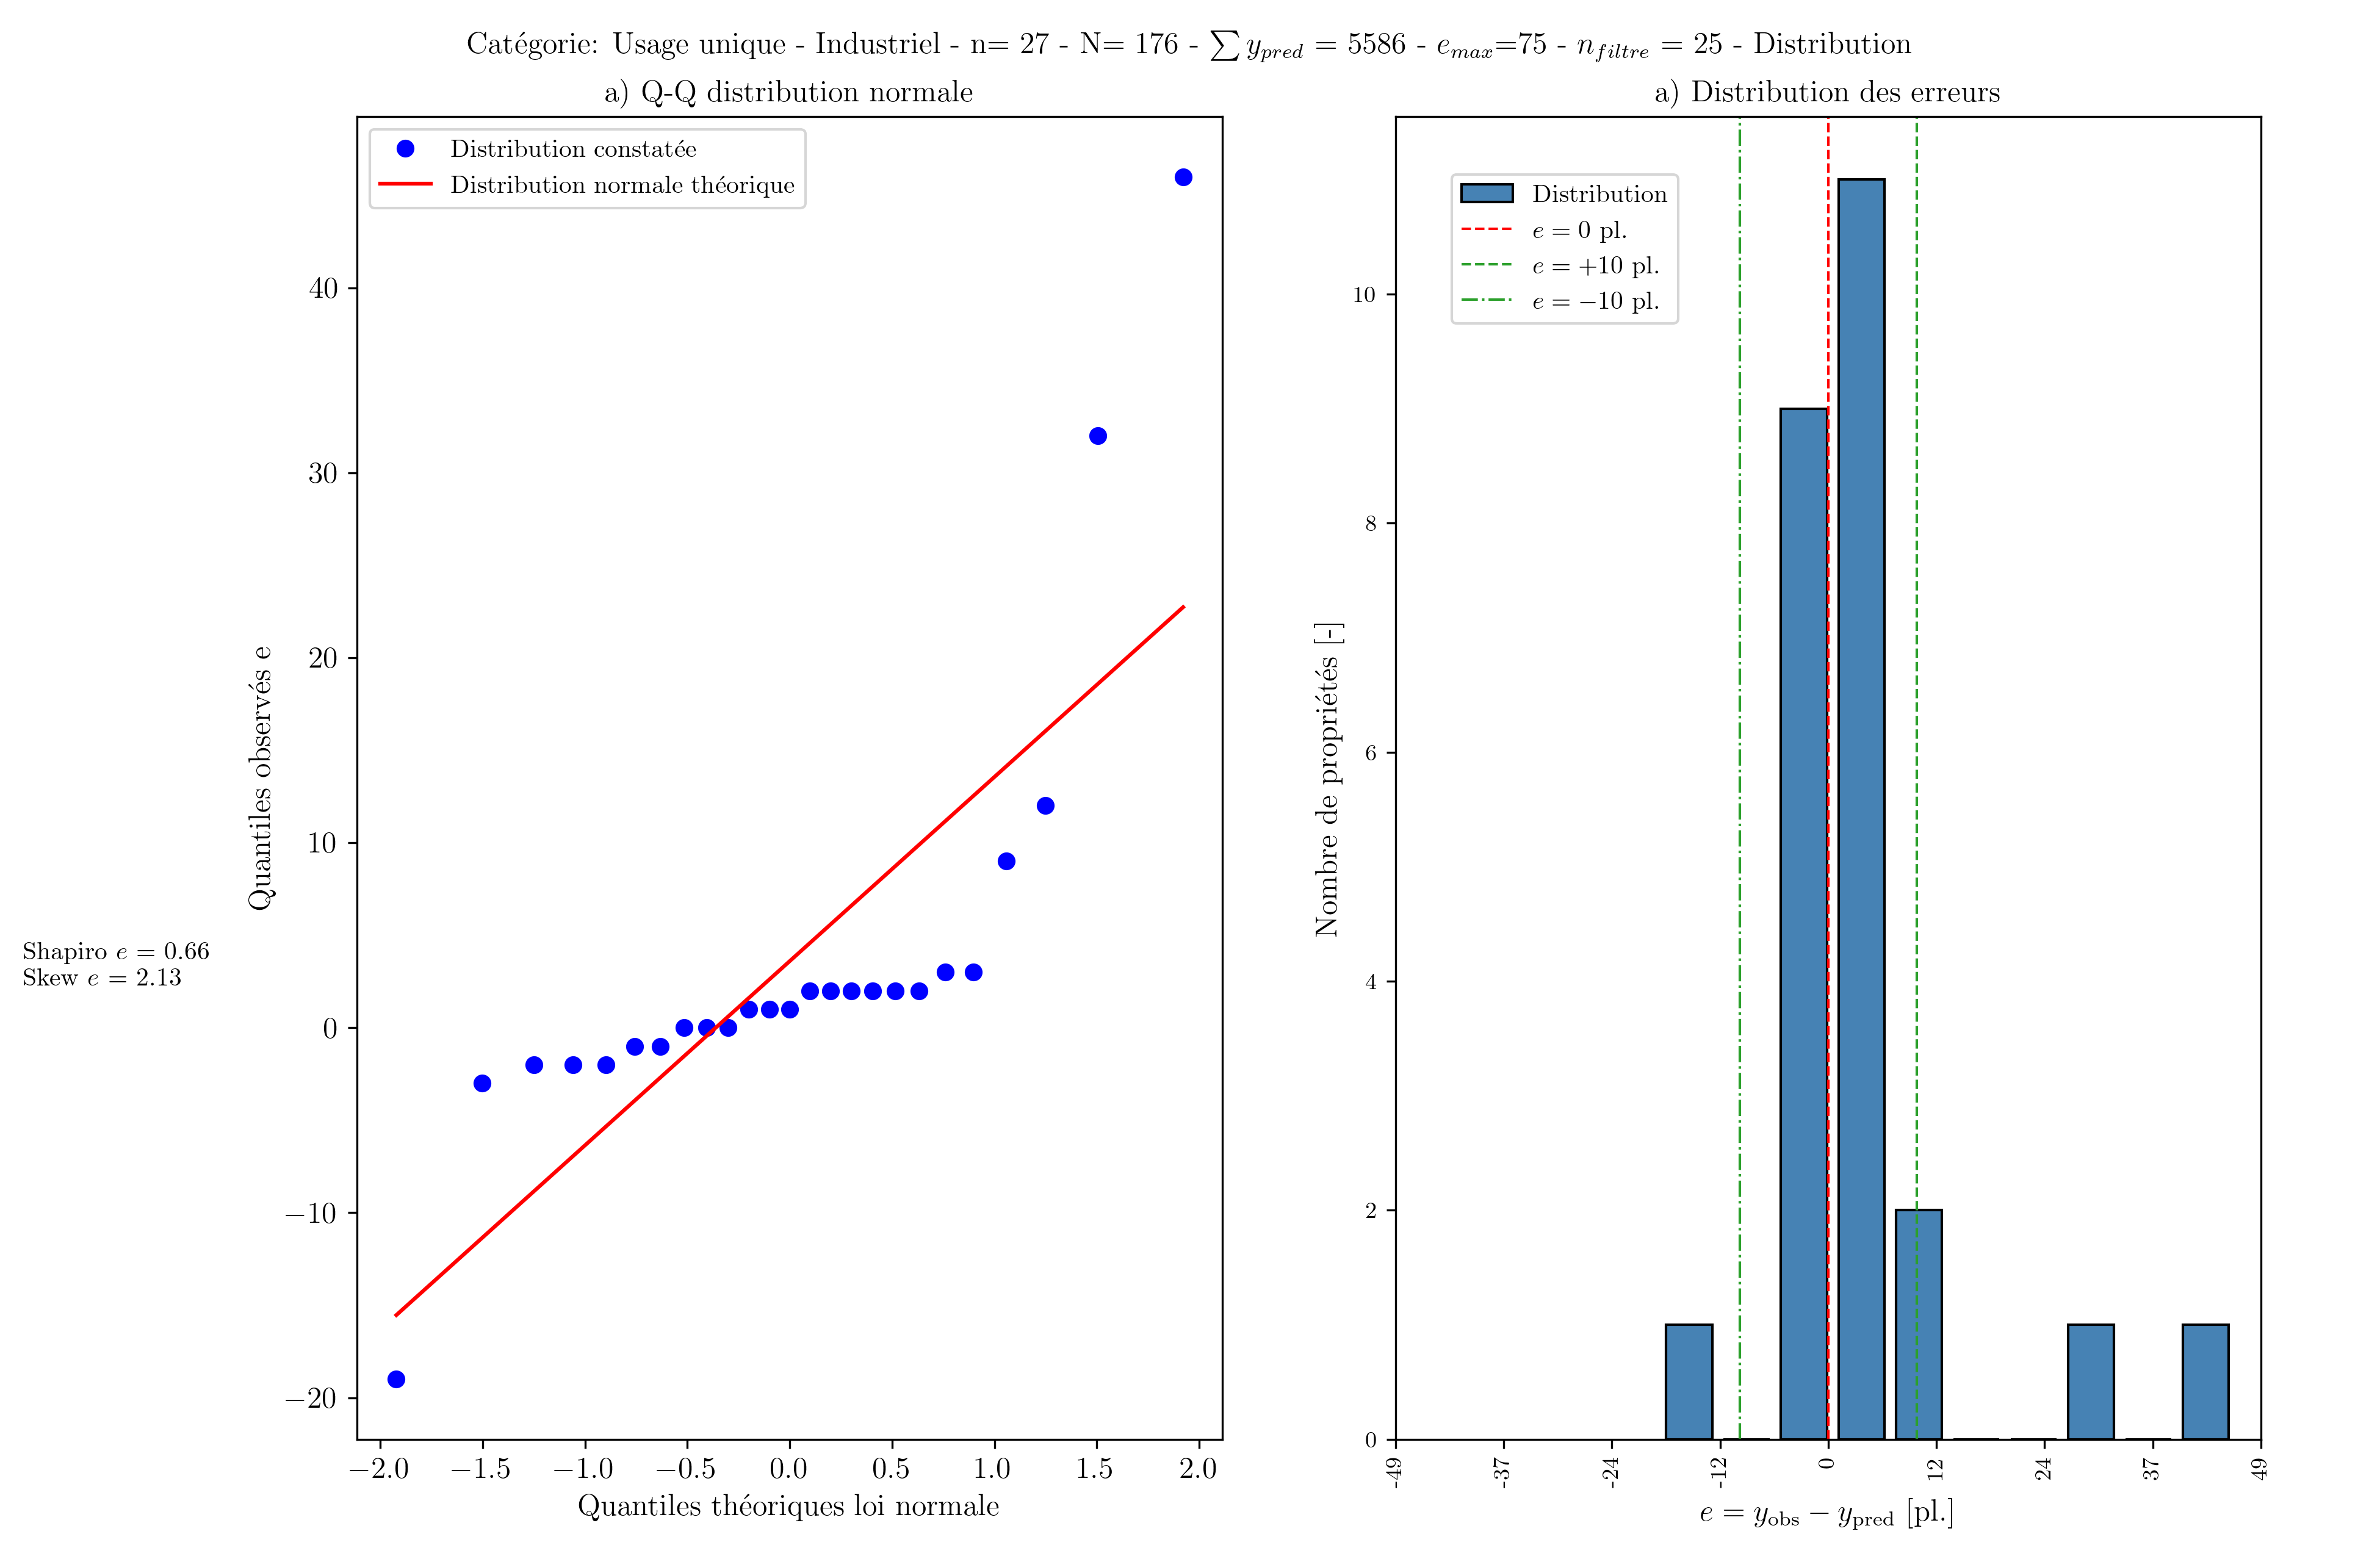
\includegraphics[width=1\linewidth]{images/int_erreur_39_e_75_se_10_pe_20_c.png}
        \caption{Distribution et normalité des erreurs pour les lots industriels}
        \label{fig:dist-erreur-norm-ind}
    \end{figure}
    \begin{figure}[H]
        \centering
        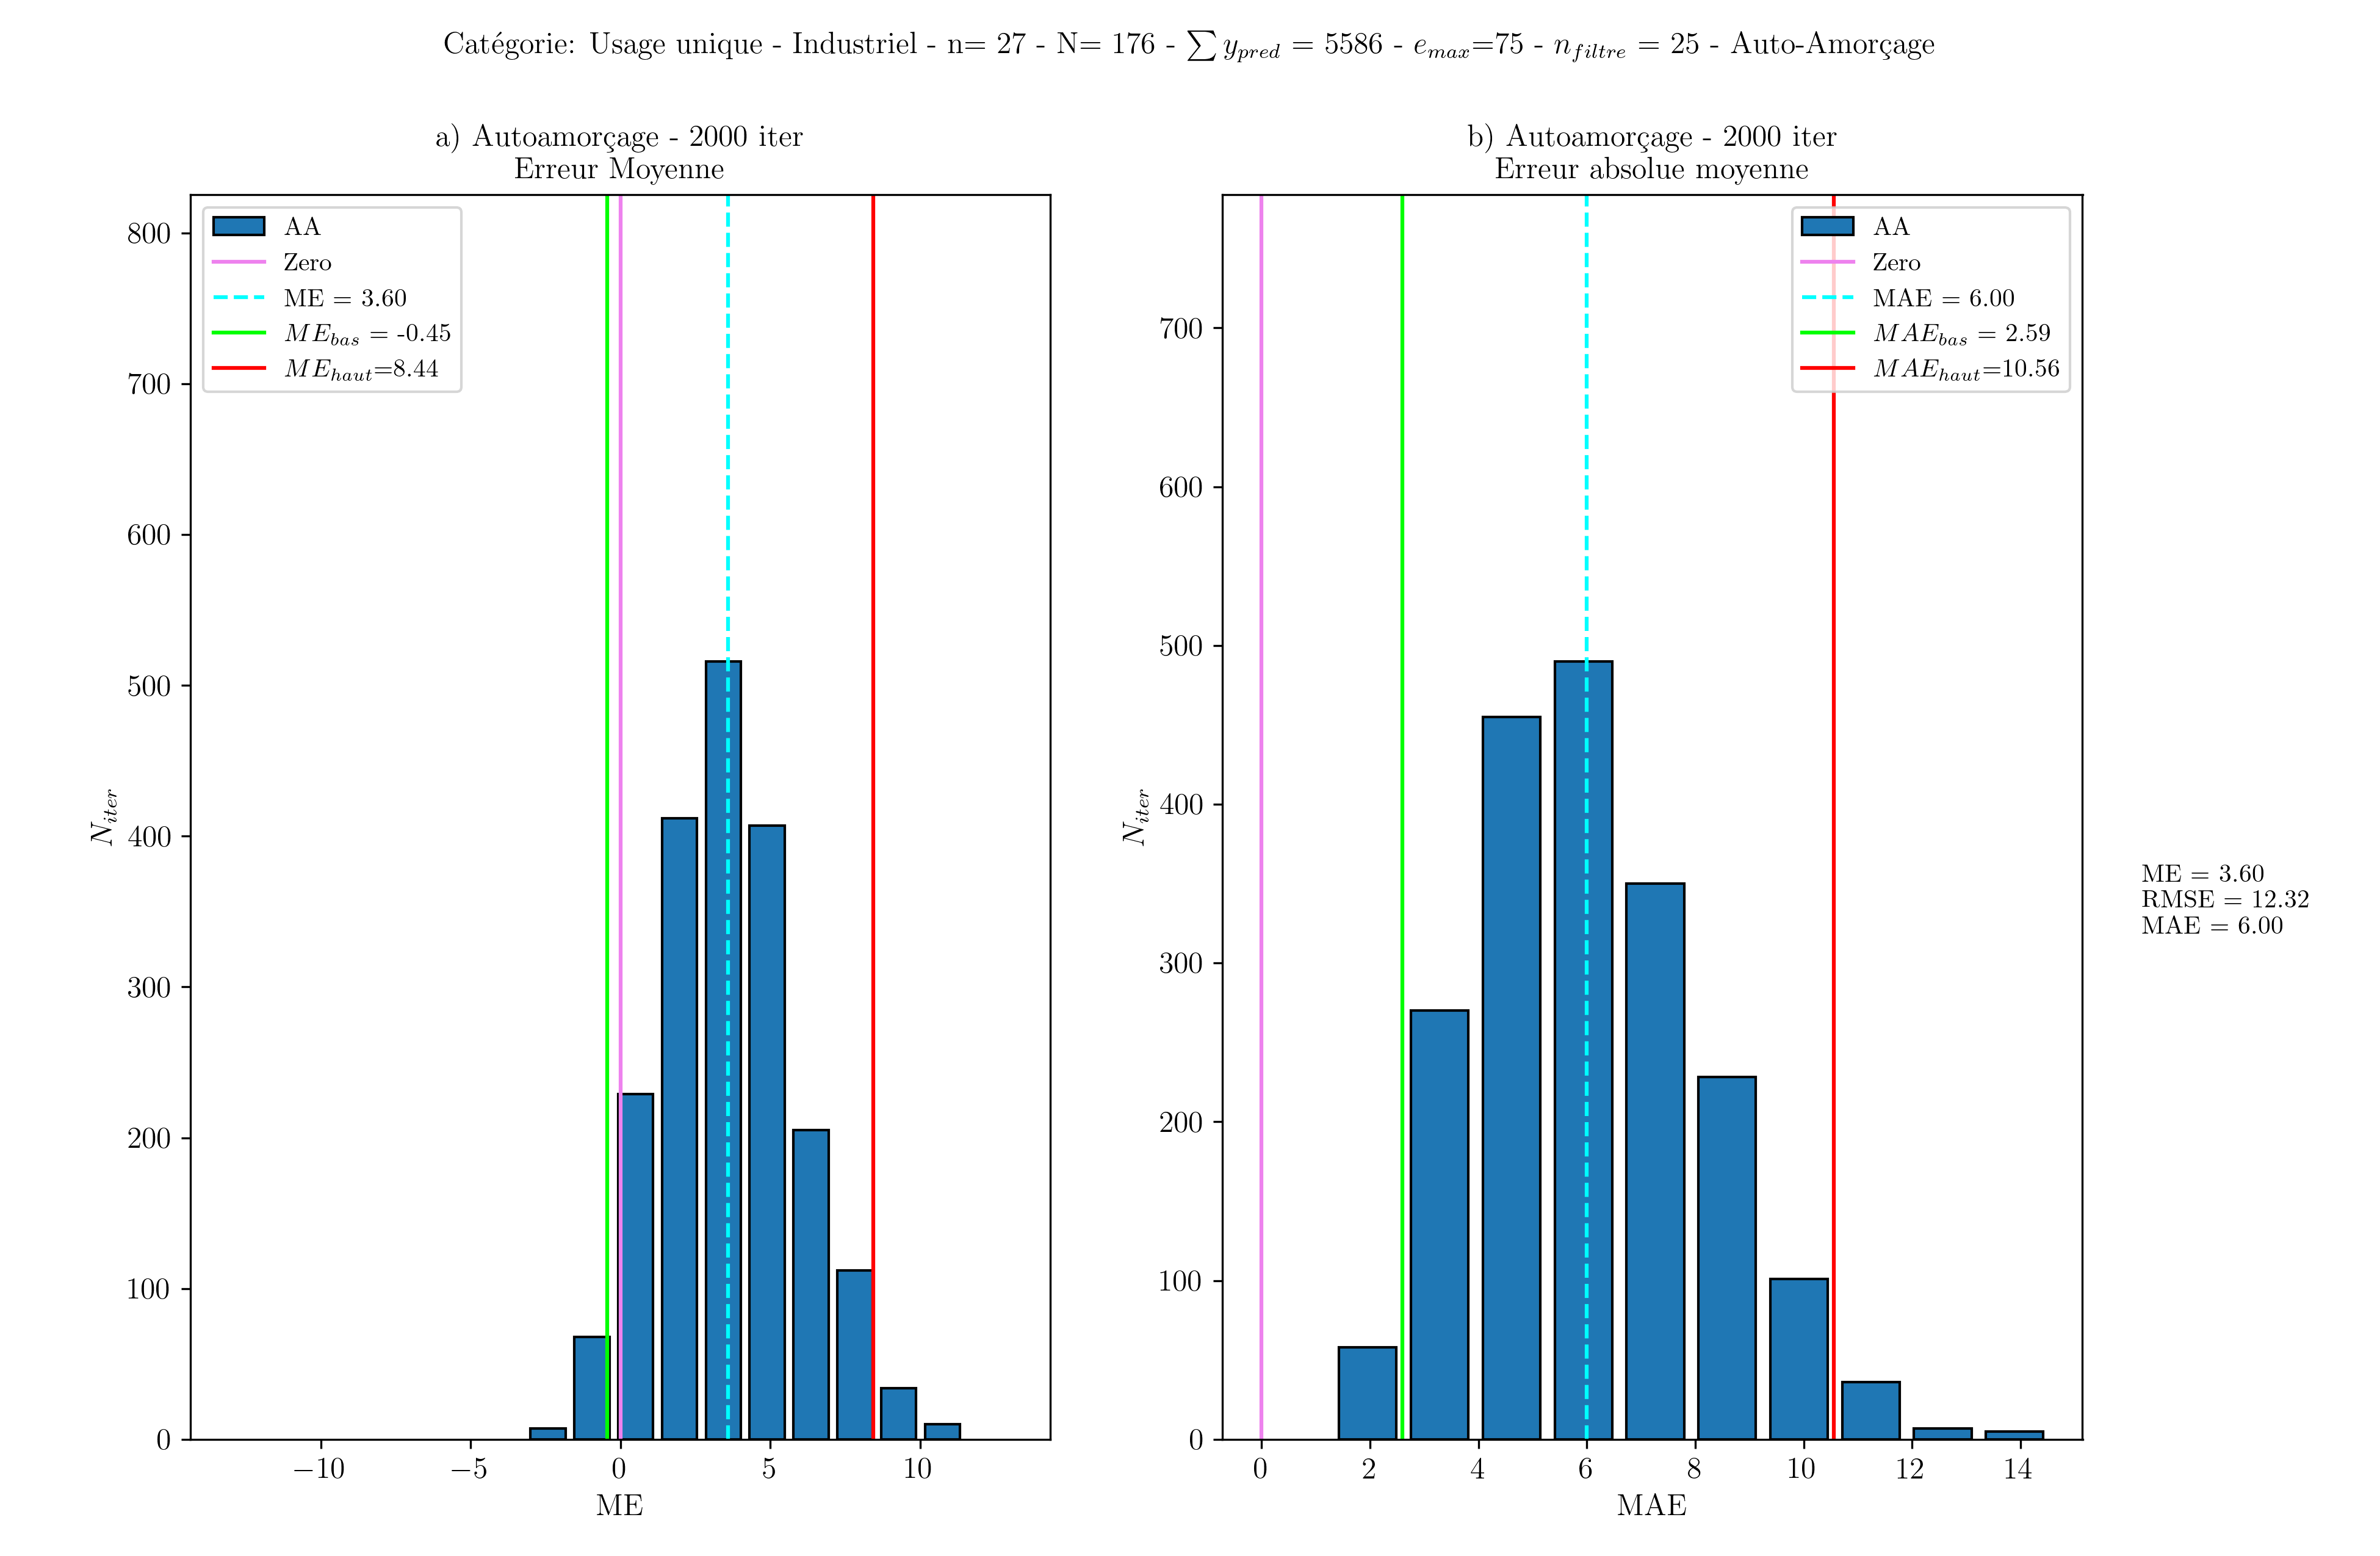
\includegraphics[width=1\linewidth]{images/int_erreur_39_e_75_se_10_pe_20_d.png}
        \caption{Distribution des métriques d'erreur après auto-amorçage pour les lots industriels}
        \label{fig:auto-amor-ind}
    \end{figure}
    \begin{figure}[H]
        \centering
        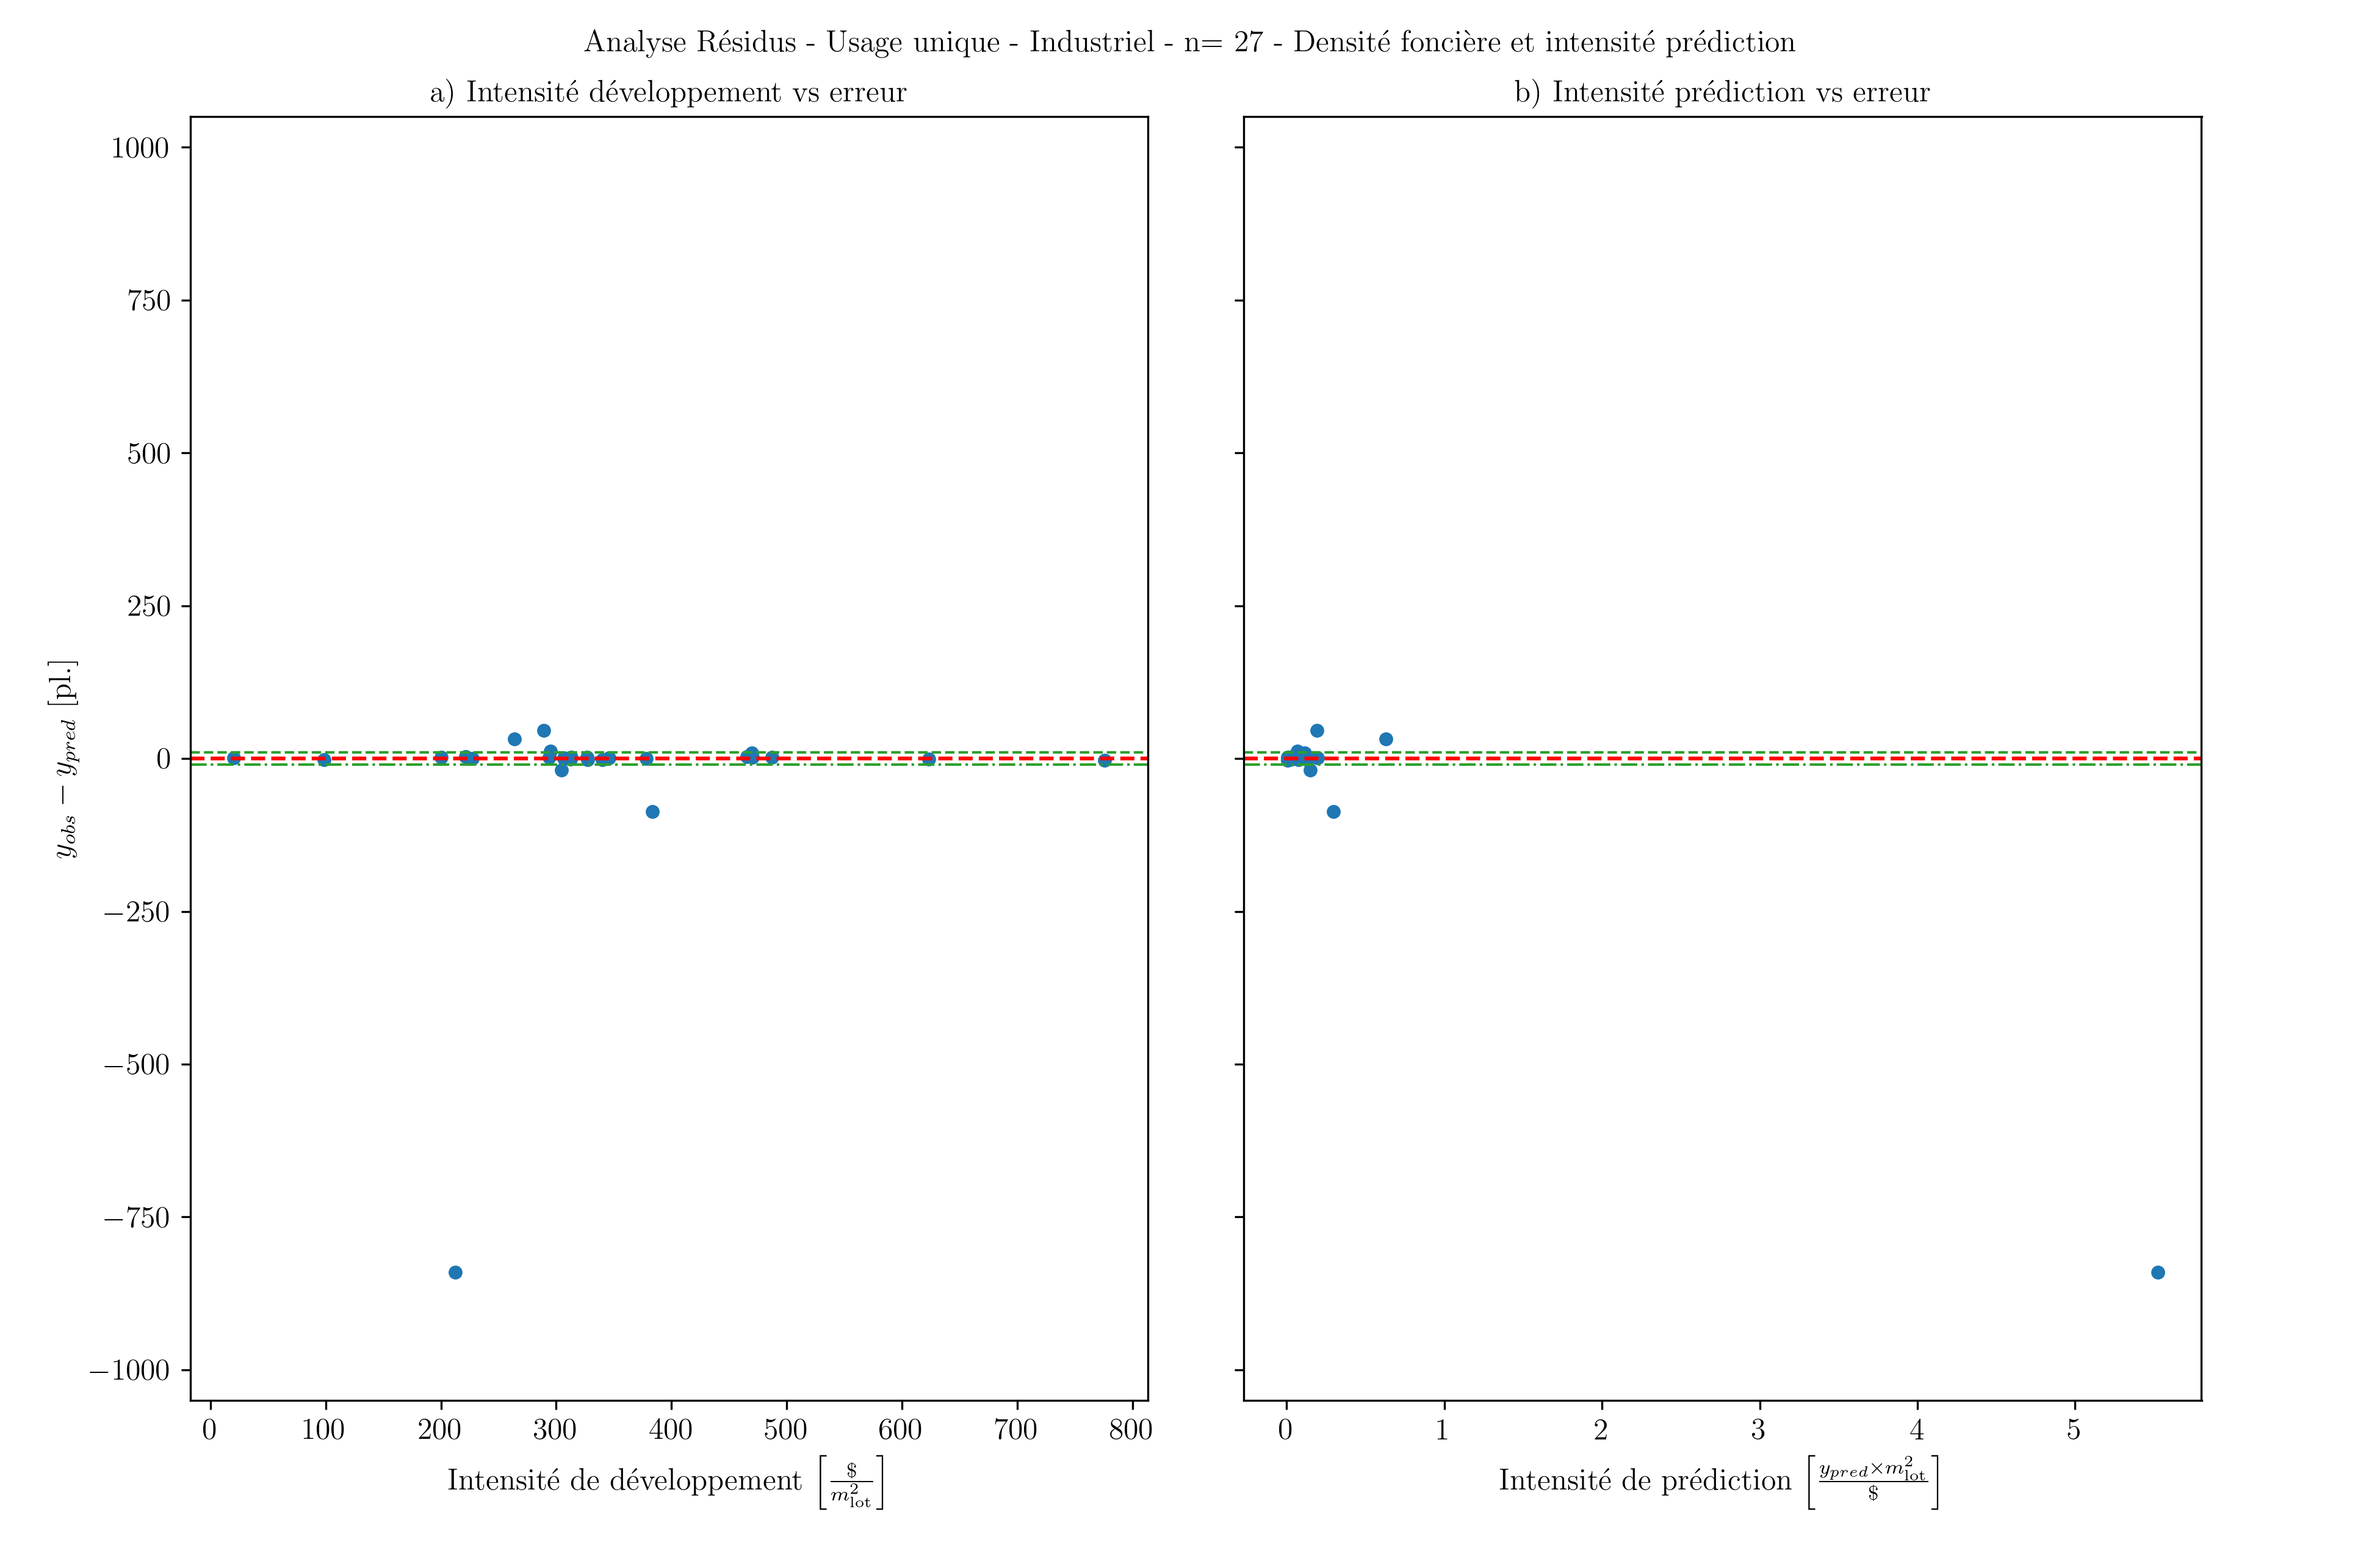
\includegraphics[width=1\linewidth]{images/ana_res_39_se_10_pe_20_e.png}
        \caption{Analyse des résidus en fonction de l'intensité de développement et l'intensité de prédiction pour les lots industriels sans filtre}
        \label{fig:ana-res-intens-ind-no-filt}
    \end{figure}
    %\begin{figure}[H]
    %    \centering
    %    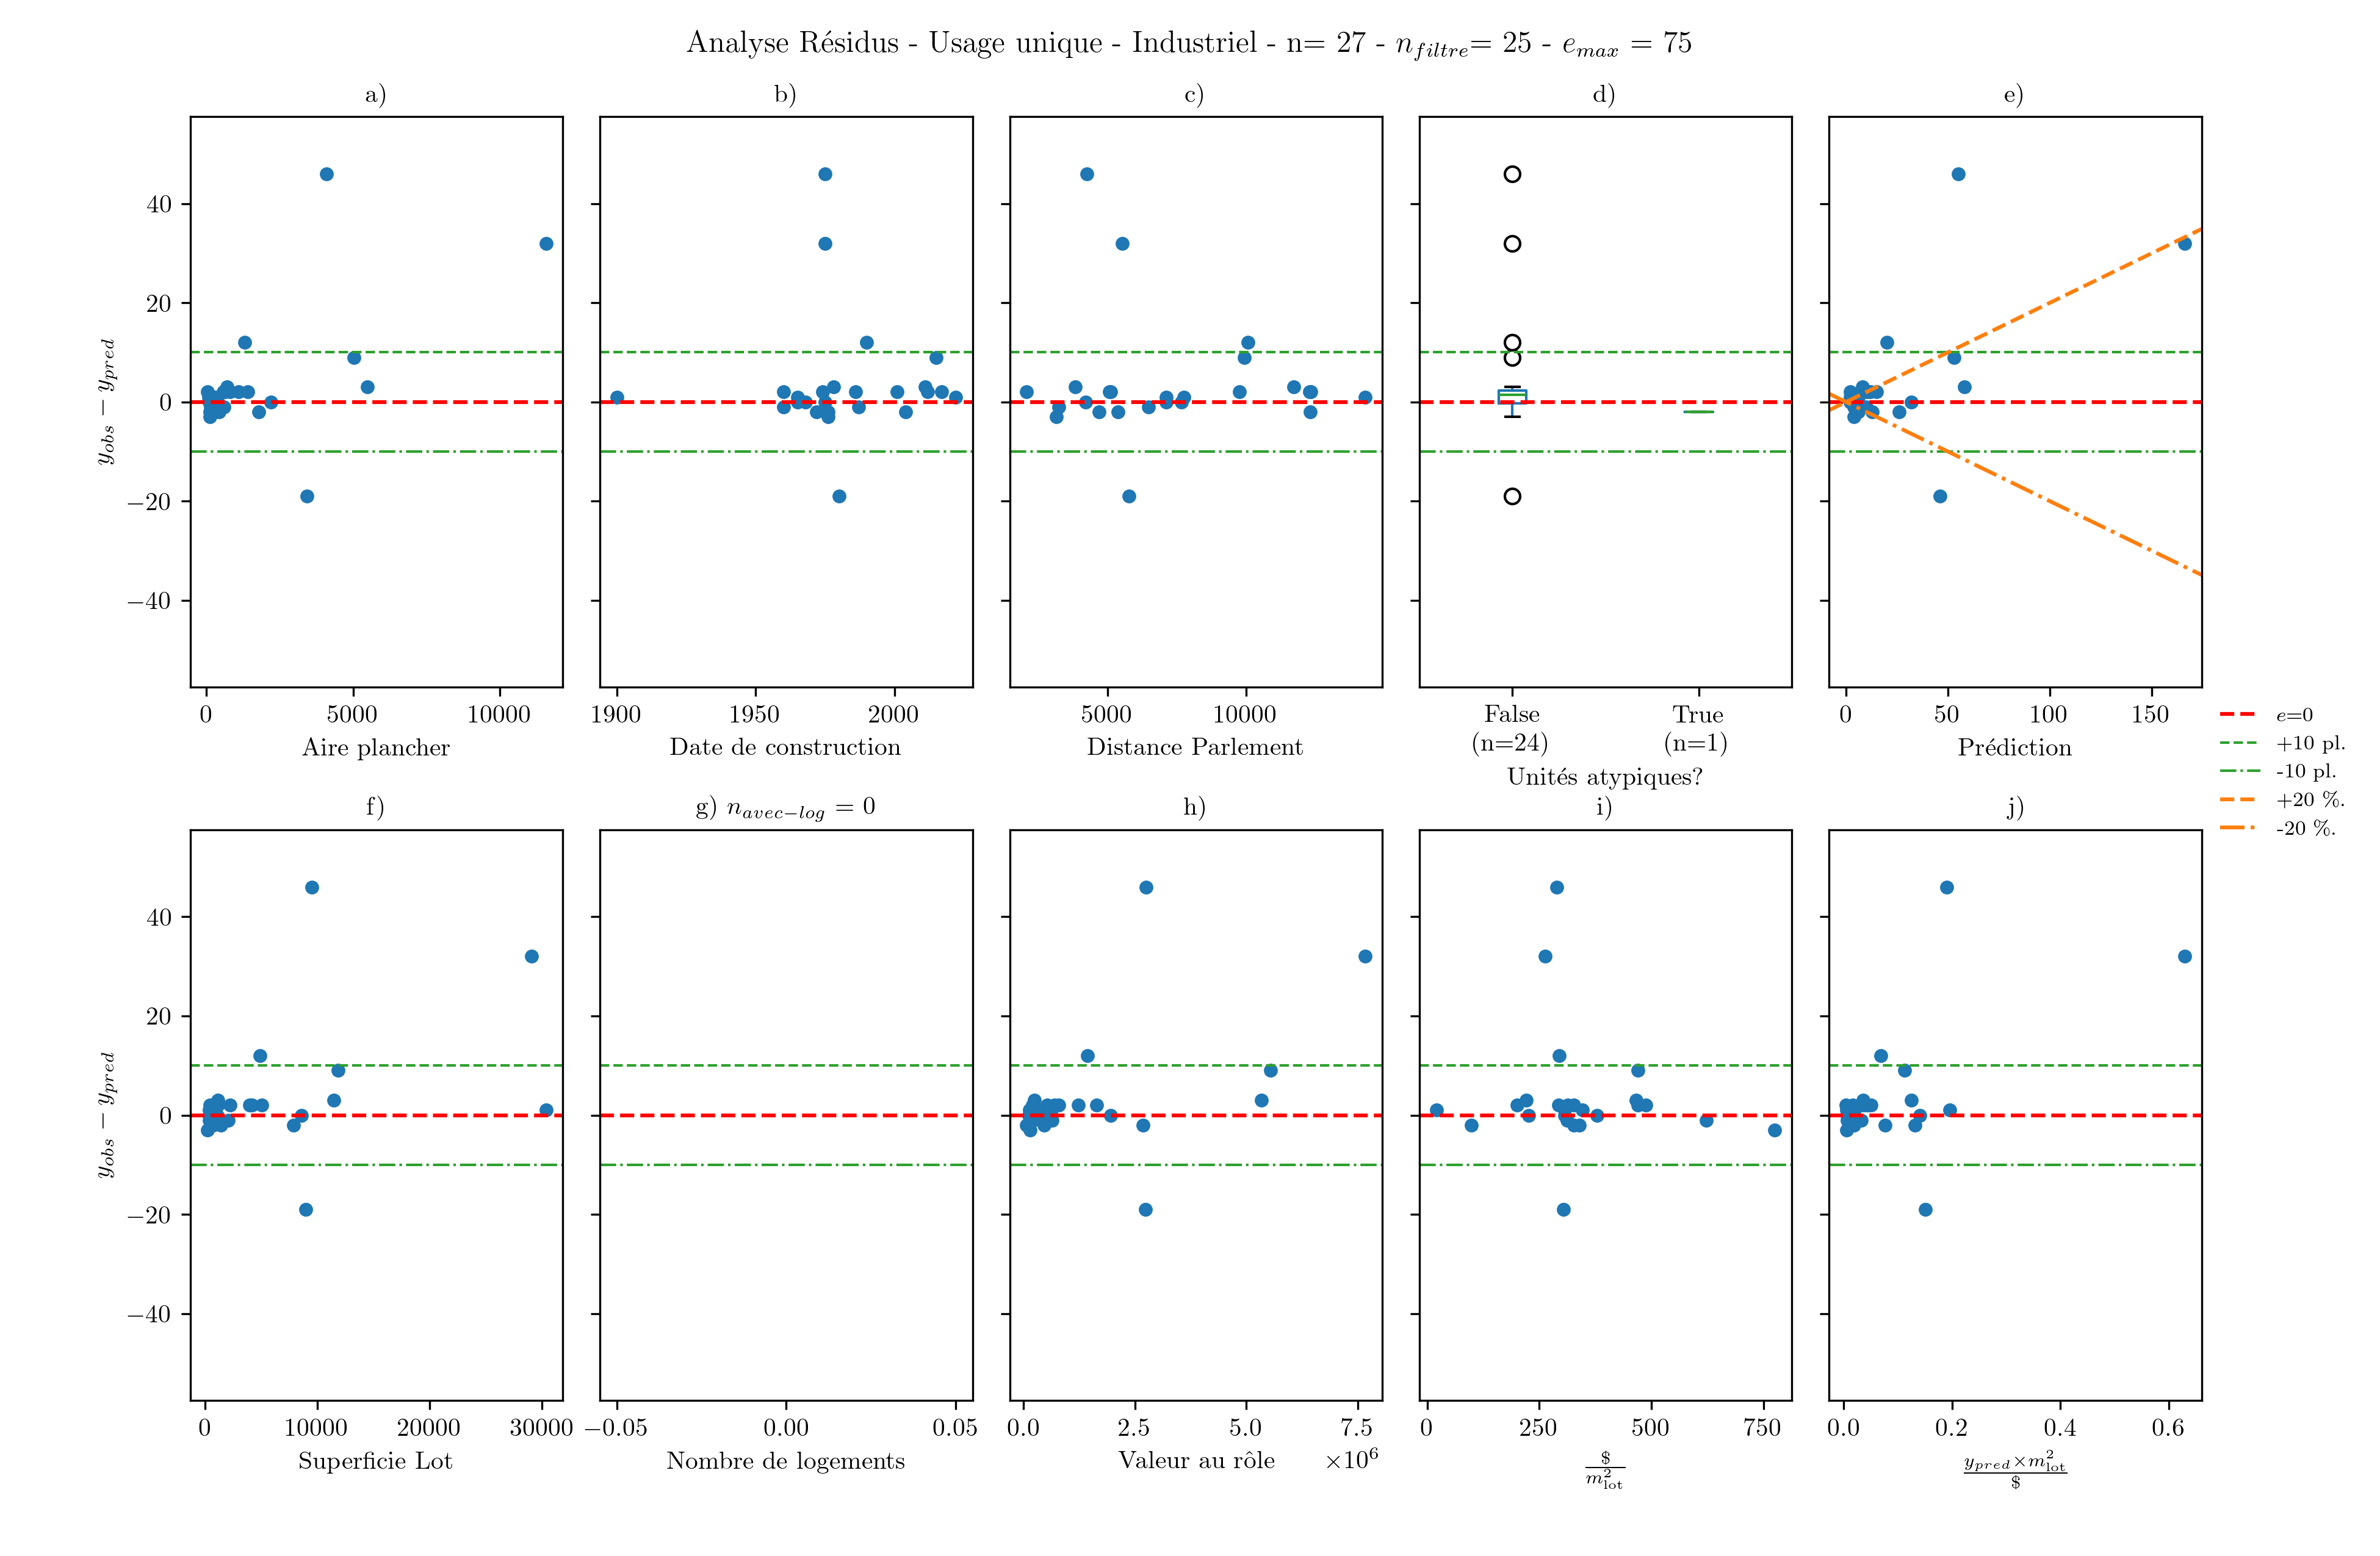
\includegraphics[scale=0.65]{images/ana_res_39_e_75_se_10_pe_20.png}
    %    \caption{Analyse des propriétés industrielles avec une erreur maximale fixée à 75 places}
    %    \label{fig:ana-residu-ind-e75}
    %\end{figure}
    \begin{figure}[H]
        \centering
        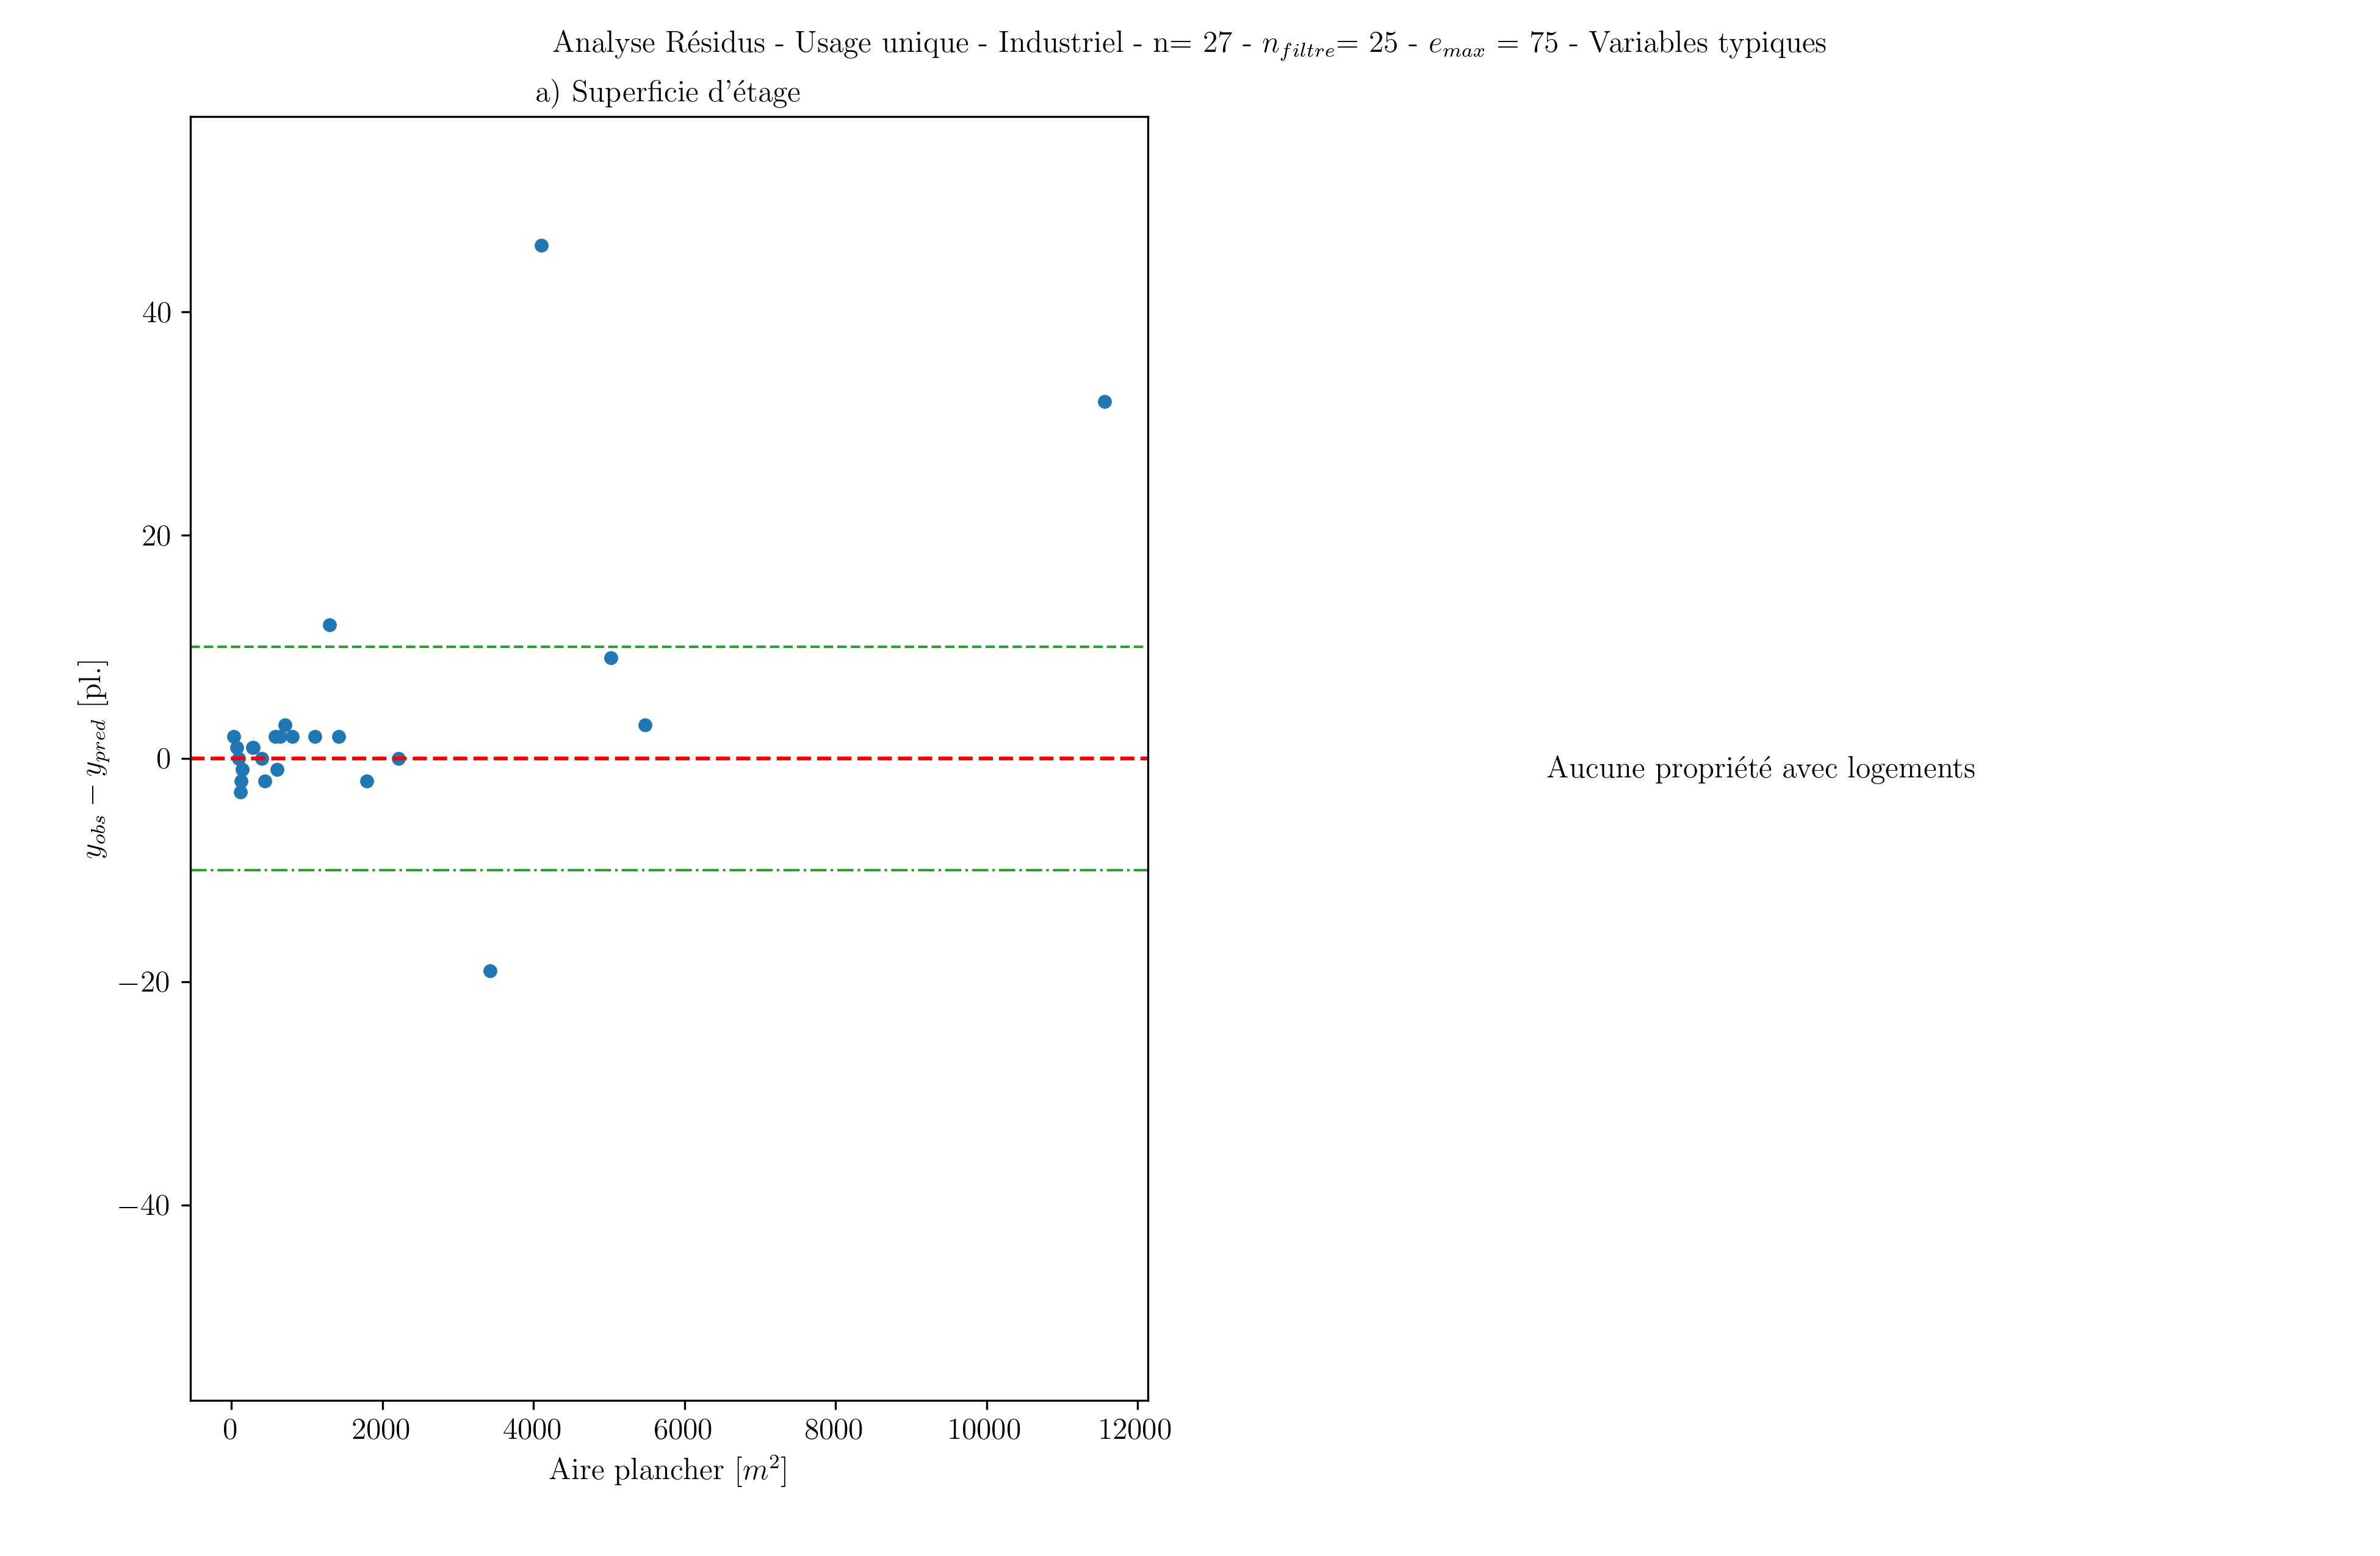
\includegraphics[width=1\linewidth]{images/ana_res_39_e_75_se_10_pe_20_a.png}
        \caption{Analyse des résidus en fonction des propriétés de construction pour les lots industriels}
        \label{fig:ana-res-prop-phys-ind}
    \end{figure}
    \begin{figure}[H]
        \centering
        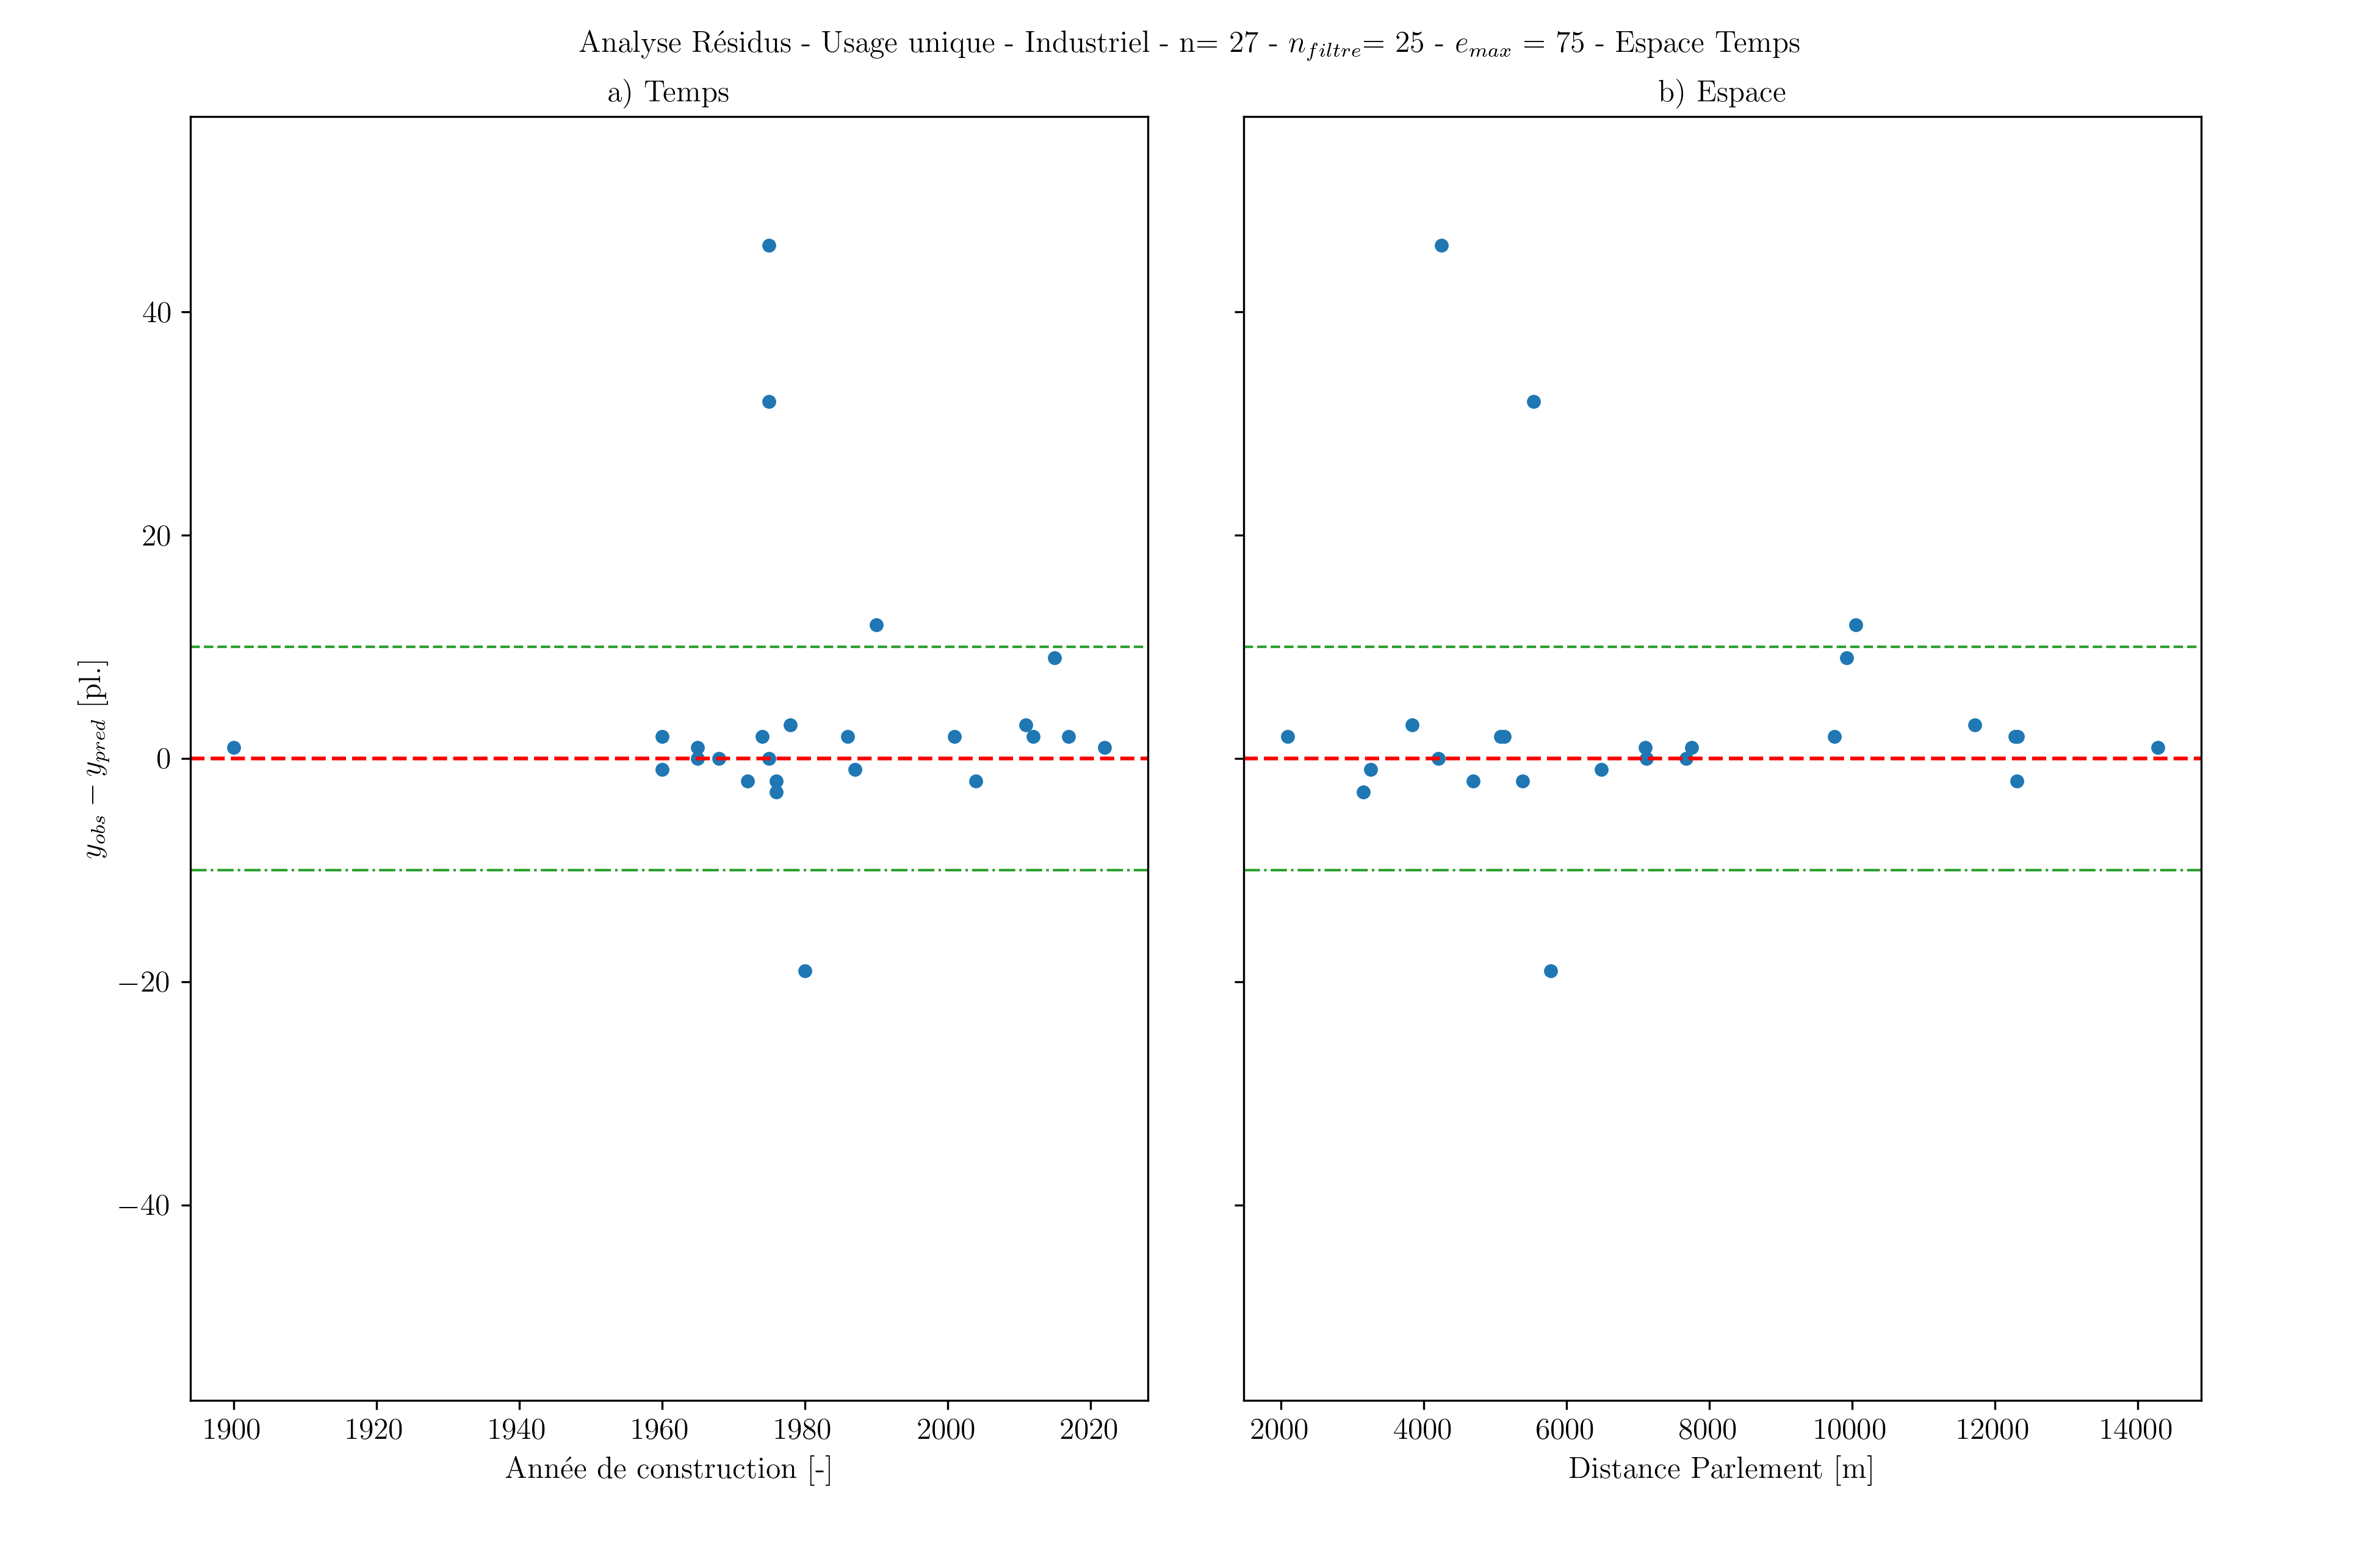
\includegraphics[width=1\linewidth]{images/ana_res_39_e_75_se_10_pe_20_b.png}
        \caption{Analyse des résidus en fonction de l'espace et de l'époque de construction pour les lots industriels}
        \label{fig:ana-res-esp-temps-ind}
    \end{figure}
    \begin{figure}[H]
        \centering
        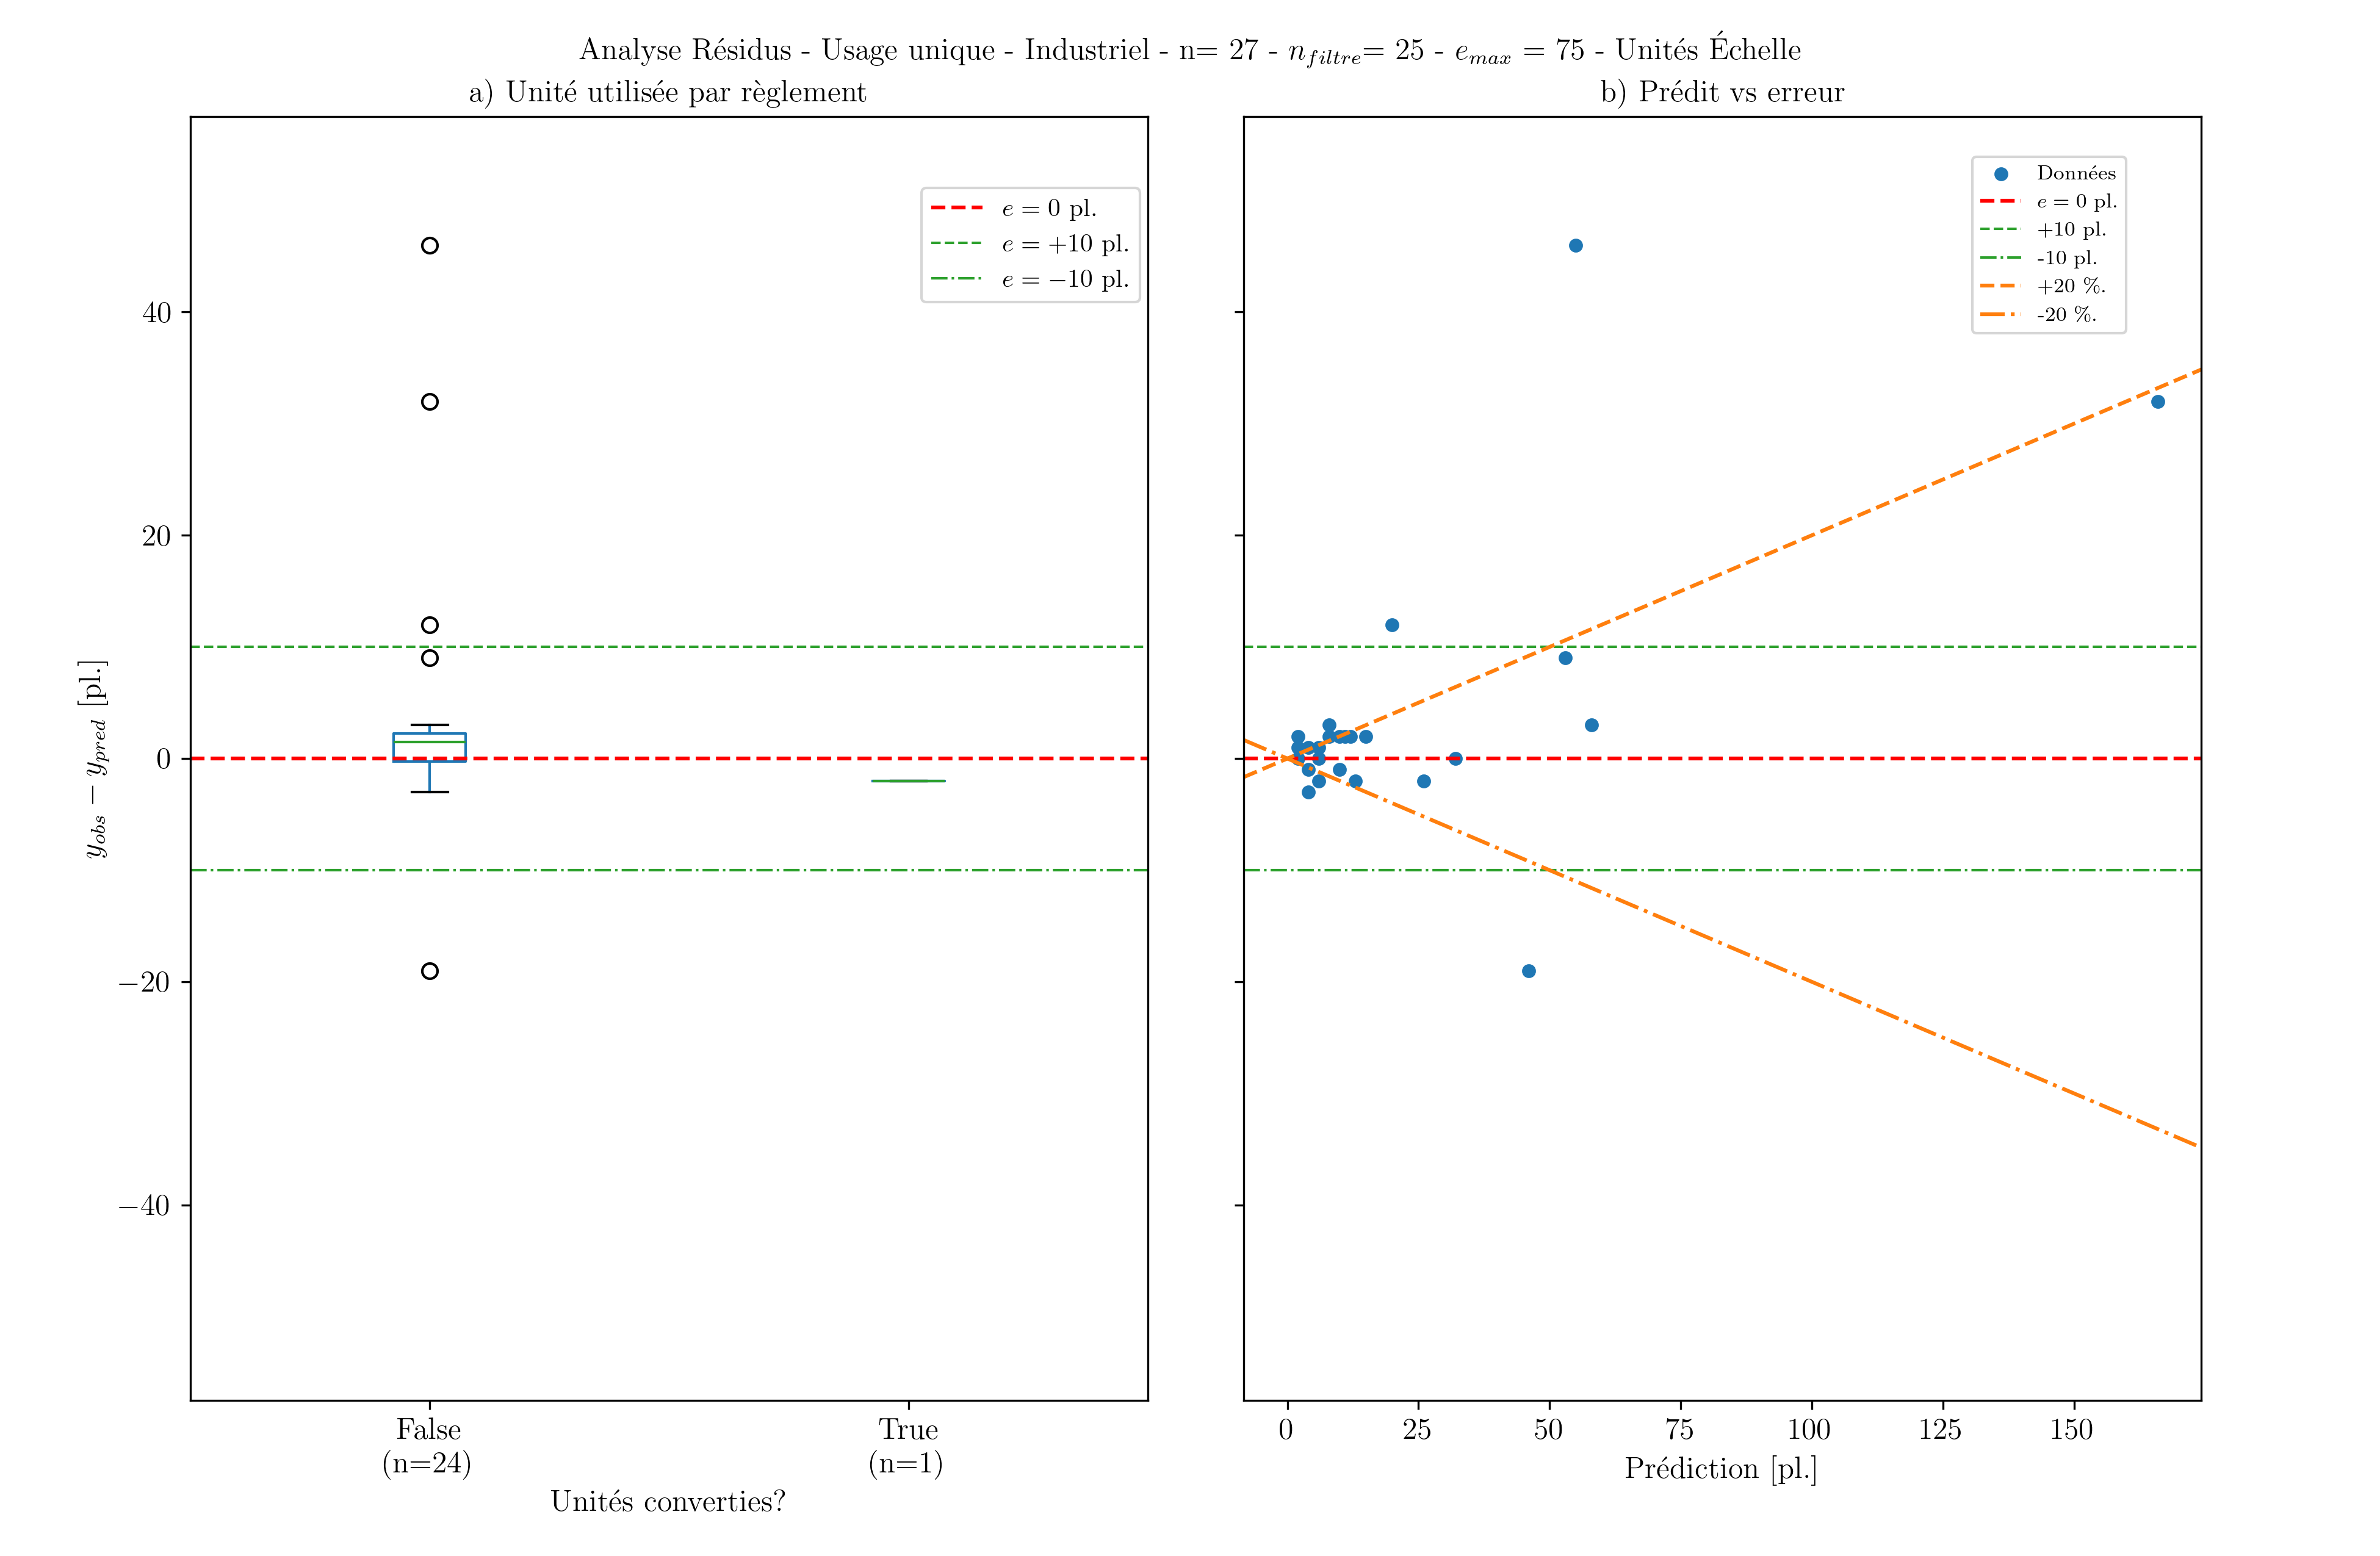
\includegraphics[width=1\linewidth]{images/ana_res_39_e_75_se_10_pe_20_c.png}
        \caption{Analyse des résidus en fonction de la prédiction et des unités de formulation pour les lots industriels}
        \label{fig:ana-res-unit-pred-ind}
    \end{figure}
    \begin{figure}[H]
        \centering
        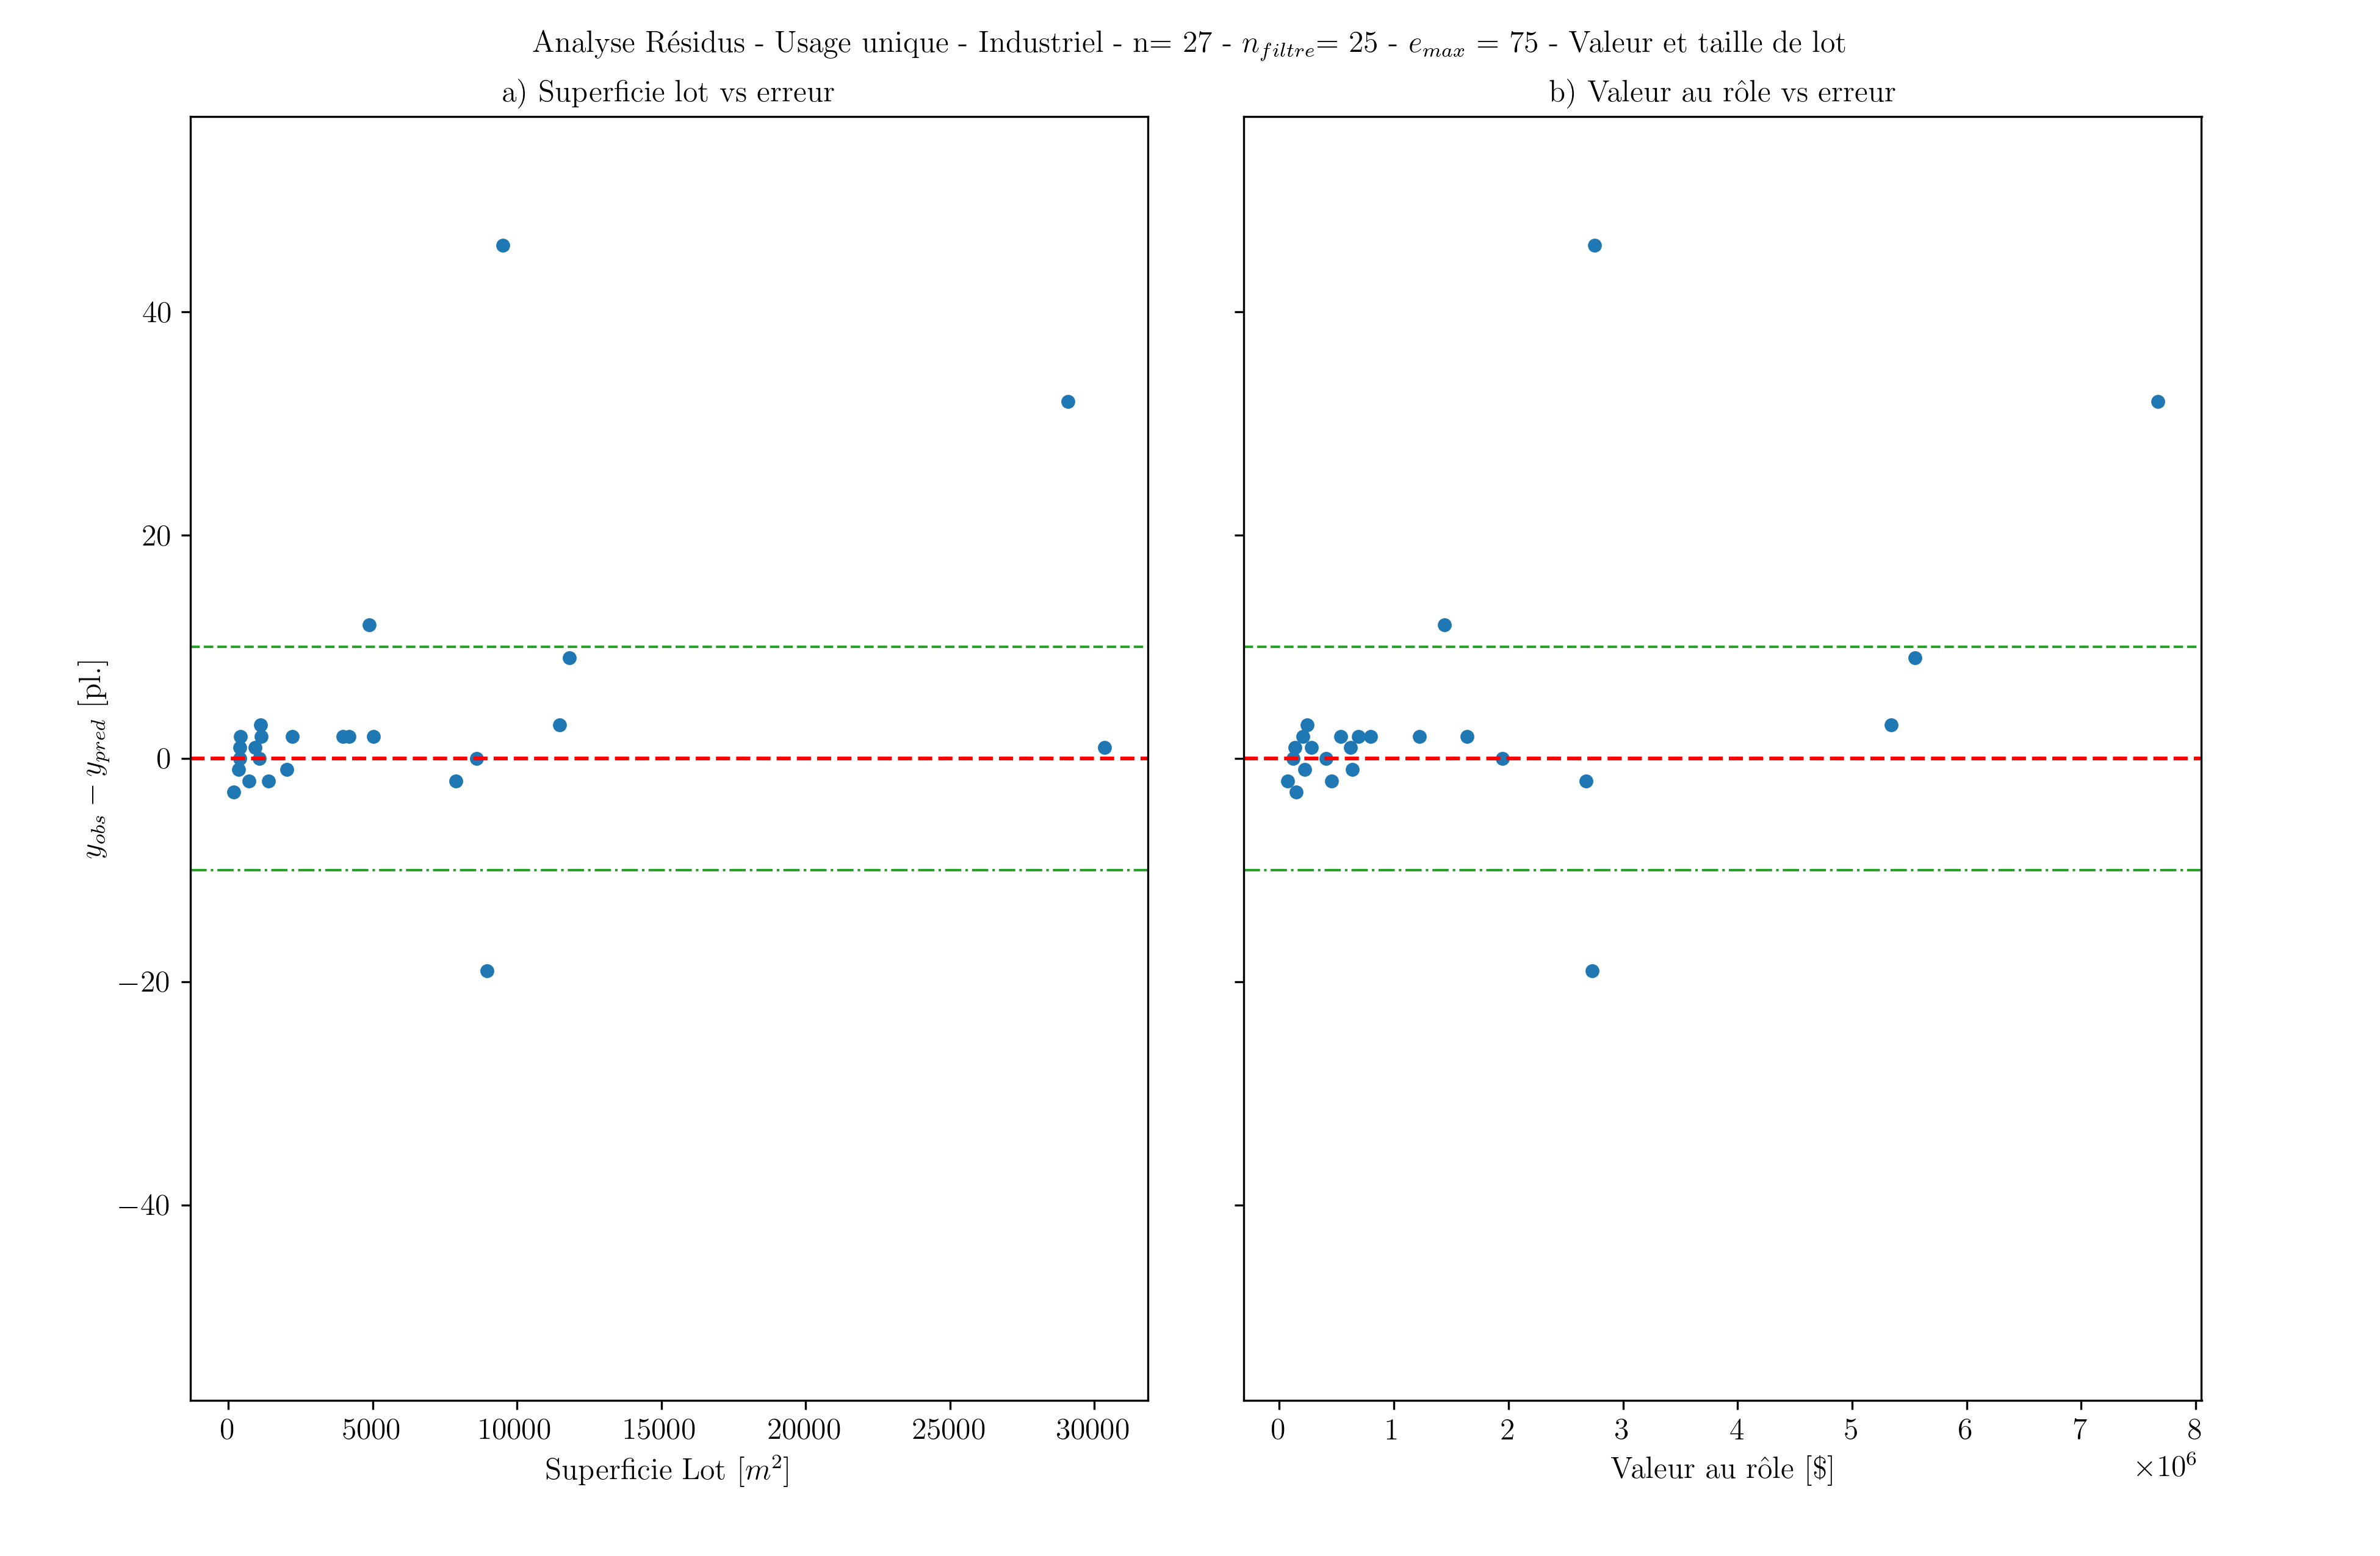
\includegraphics[width=1\linewidth]{images/ana_res_39_e_75_se_10_pe_20_d.png}
        \caption{Analyse des résidus en fonction de la superficie du lot et de la valeur pour les lots industriels}
        \label{fig:ana-res-sup-val-ind}
    \end{figure}
    \begin{figure}[H]
        \centering
        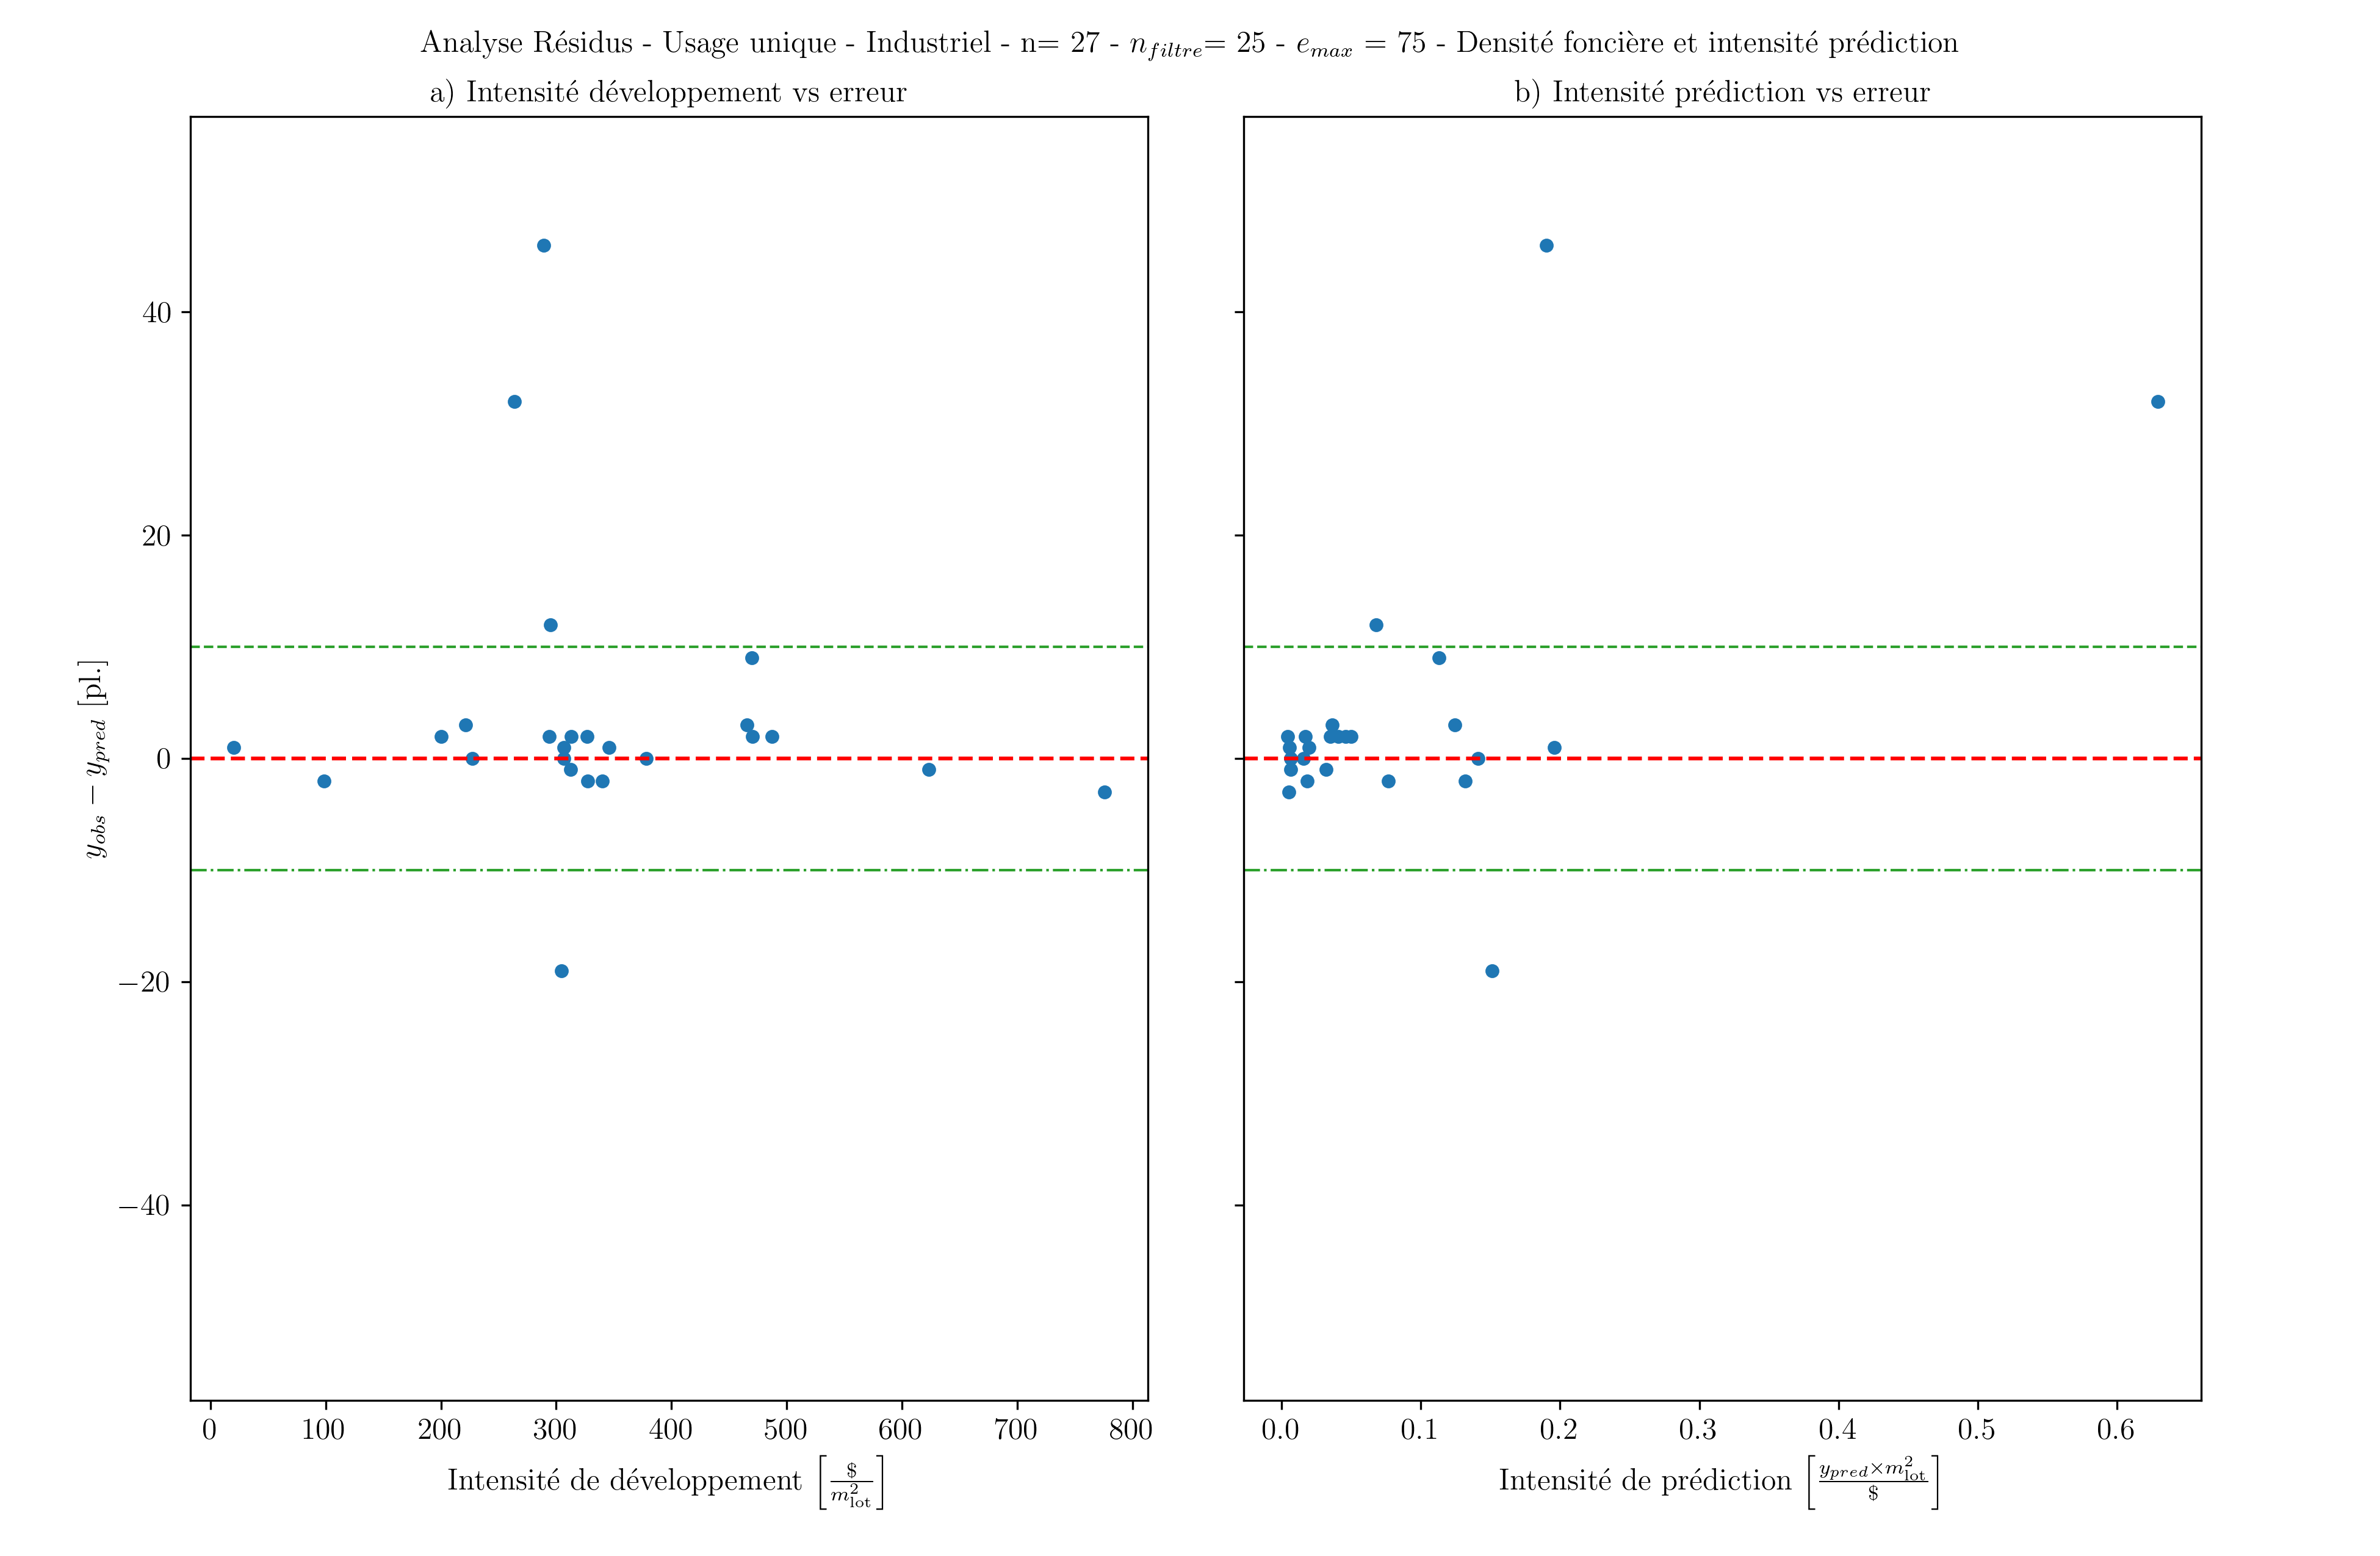
\includegraphics[width=1\linewidth]{images/ana_res_39_e_75_se_10_pe_20_e.png}
        \caption{Analyse des résidus en fonction de l'intensité de développement et l'intensité de prédiction pour les lots industriels}
        \label{fig:ana-res-intens-ind}
    \end{figure}
\end{landscape}
\subsection{Assemblée et récréation}
Trente lots de type assemblée et récréation ont été échantillonnés. L'enjeu principal est que cette catégorie regroupe des types de propriétés hétérogènes qui incluent des musées, mais aussi des terrains de jeu et des parcs qui ne se prêtent pas particulièrement bien à être regroupés. Le principal prédicteur d'erreur dans cette catégorie est l'utilisation d'unités qui nécessitent une conversion. L'erreur en fonction de l'unité de formulation du règlement est montrée à la figure \ref{fig:boxplot-erreur-assemblee-unite}. Un exemple de requête pour trouver les lots requis est donné à l'annexe \ref{ann:recerche-inv-par-unite}. Le nombre de sièges est utilisé pour prédire le nombre de places sur 23 lots dans la ville.\par

\begin{figure}[H]
    \centering
    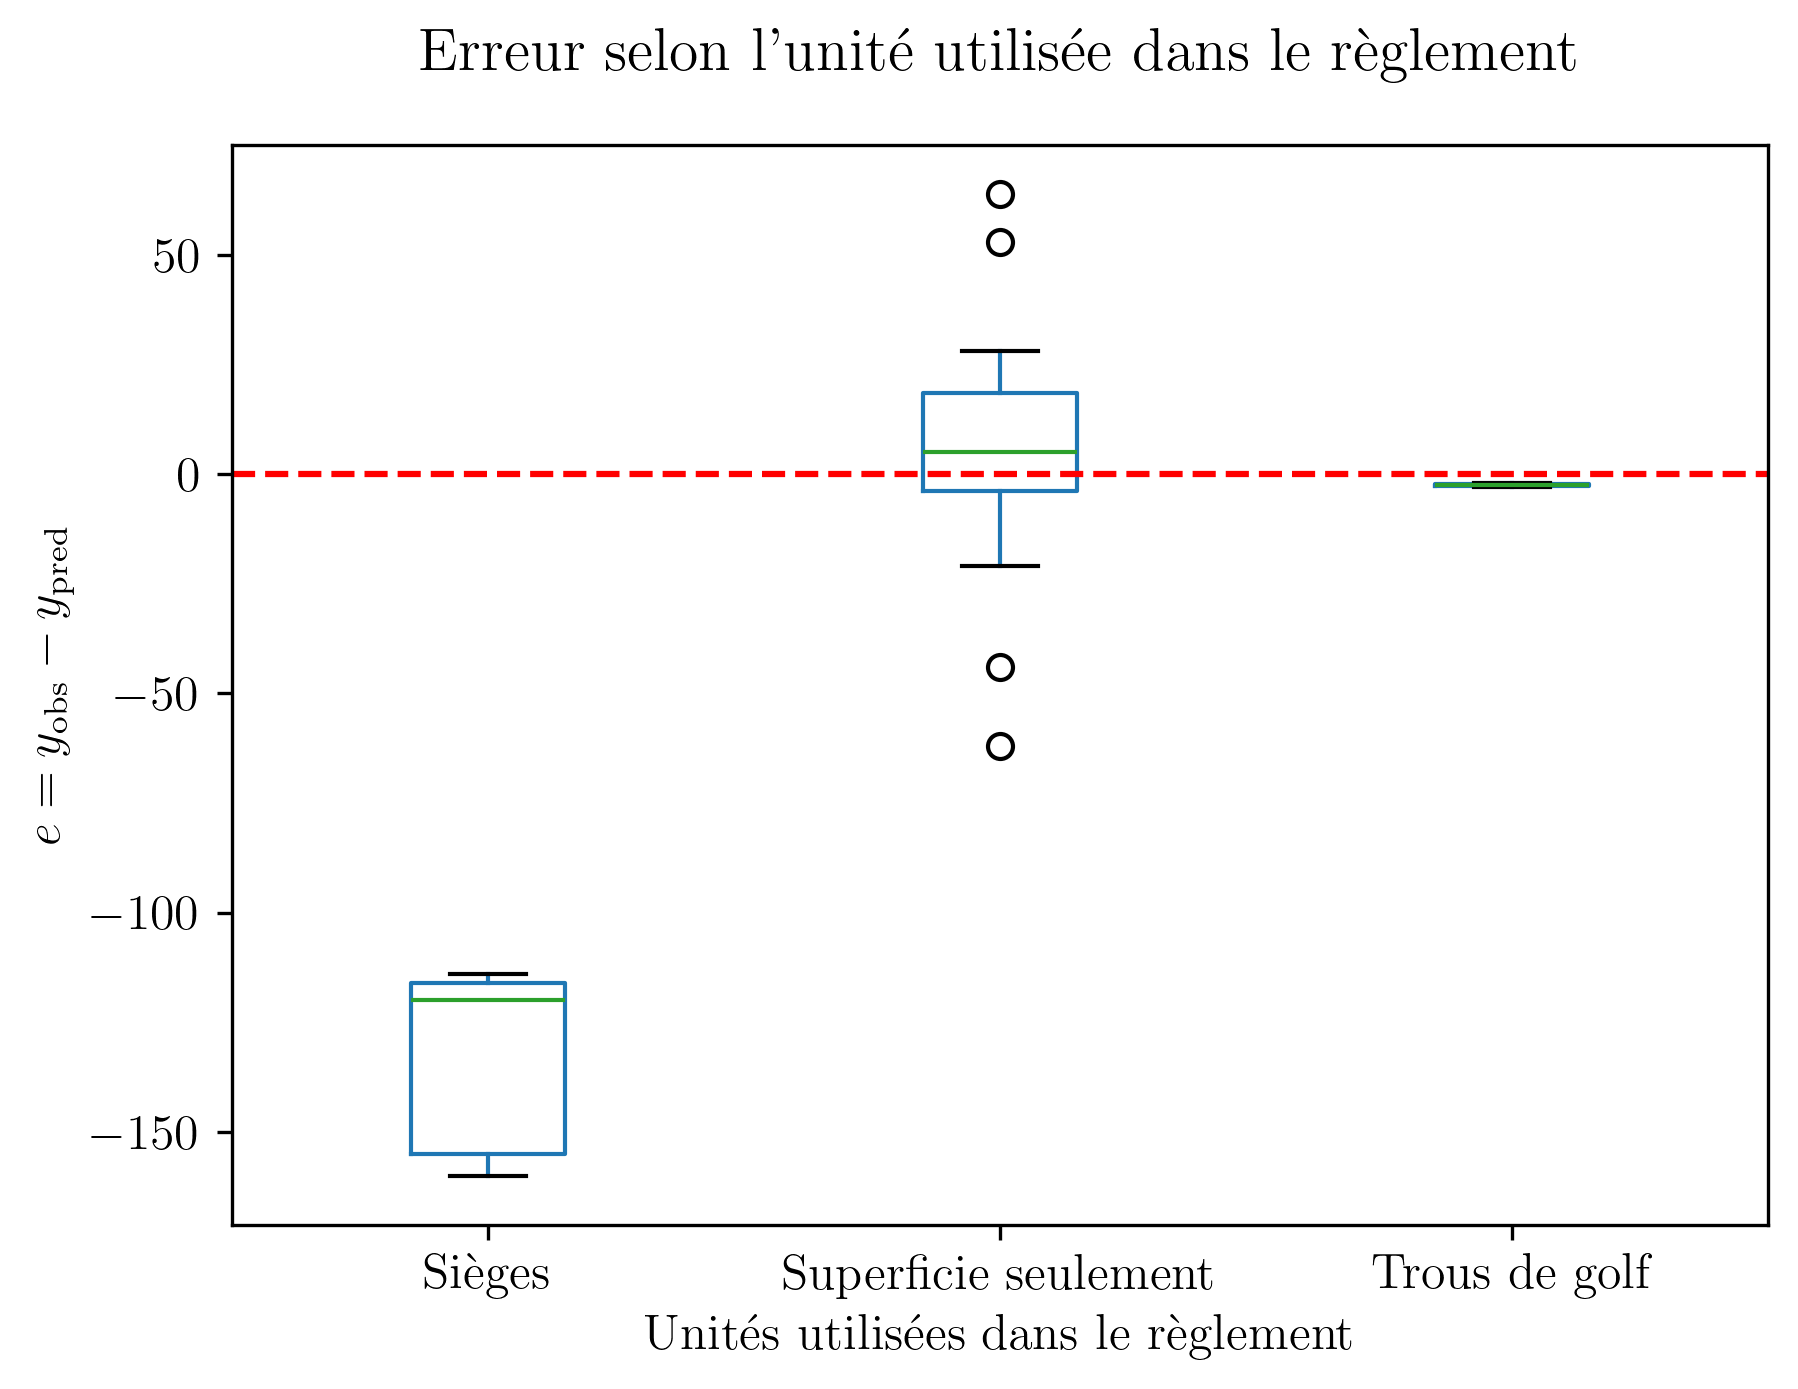
\includegraphics[width=0.8\linewidth]{images/boxplot_error_by_category_42.png}
    \caption{Erreur de la catégorie assemblée selon l'unité de formulation du règlement}
    \label{fig:boxplot-erreur-assemblee-unite}
\end{figure}
Les lots dont la valeur est inférieure à 100\$ ont été filtrés pour la figure \ref{fig:ana-res-intens-ass}, car un des lots de validation avait une valeur au rôle de 2\$ menant à des enjeux de lisibilité pour le graphique.
\begin{landscape}
    %\begin{figure}
    %    \centering
    %    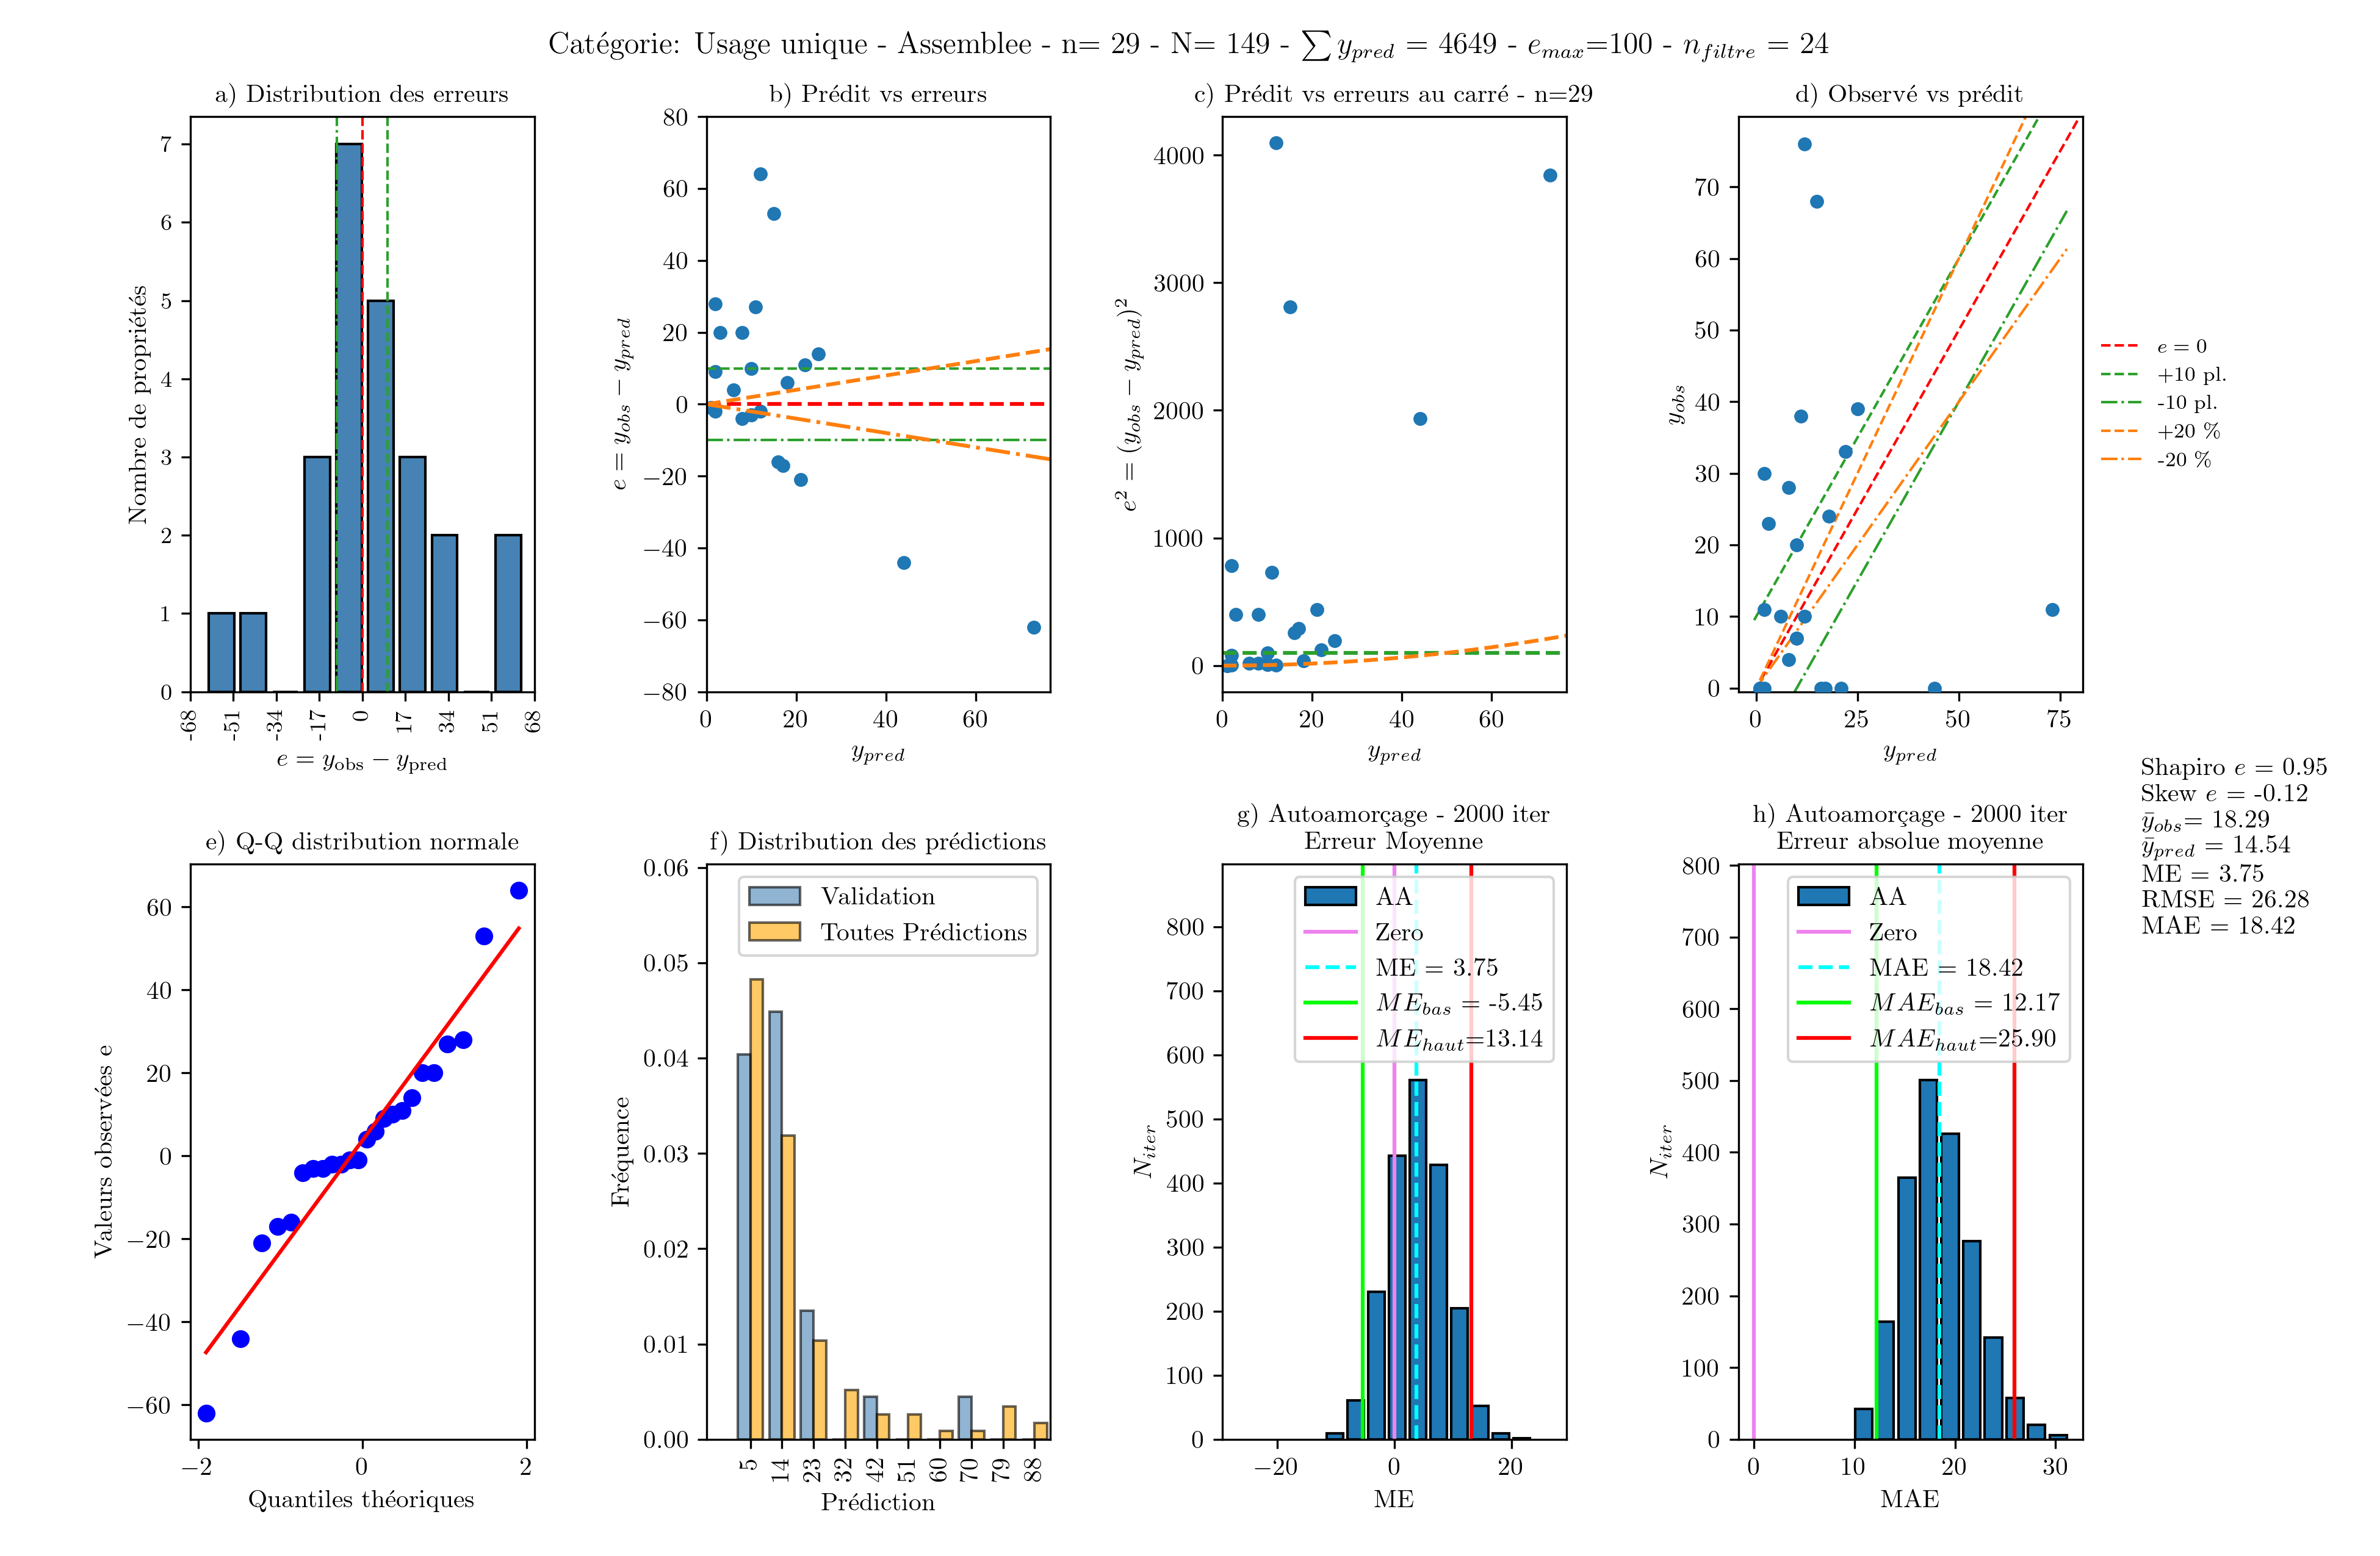
\includegraphics[scale=0.65]{images/int_erreur_42_e_100_se_10_pe_20.png}
    %    \caption{Distribution et intervalles d'erreurs pour les lots de récréation et d'assemblée avec une erreur %maximale fixée à 100 places}
    %    \label{fig:intervals-dis-val-assem-e100}
    %\end{figure}
    \begin{figure}[H]
        \centering
        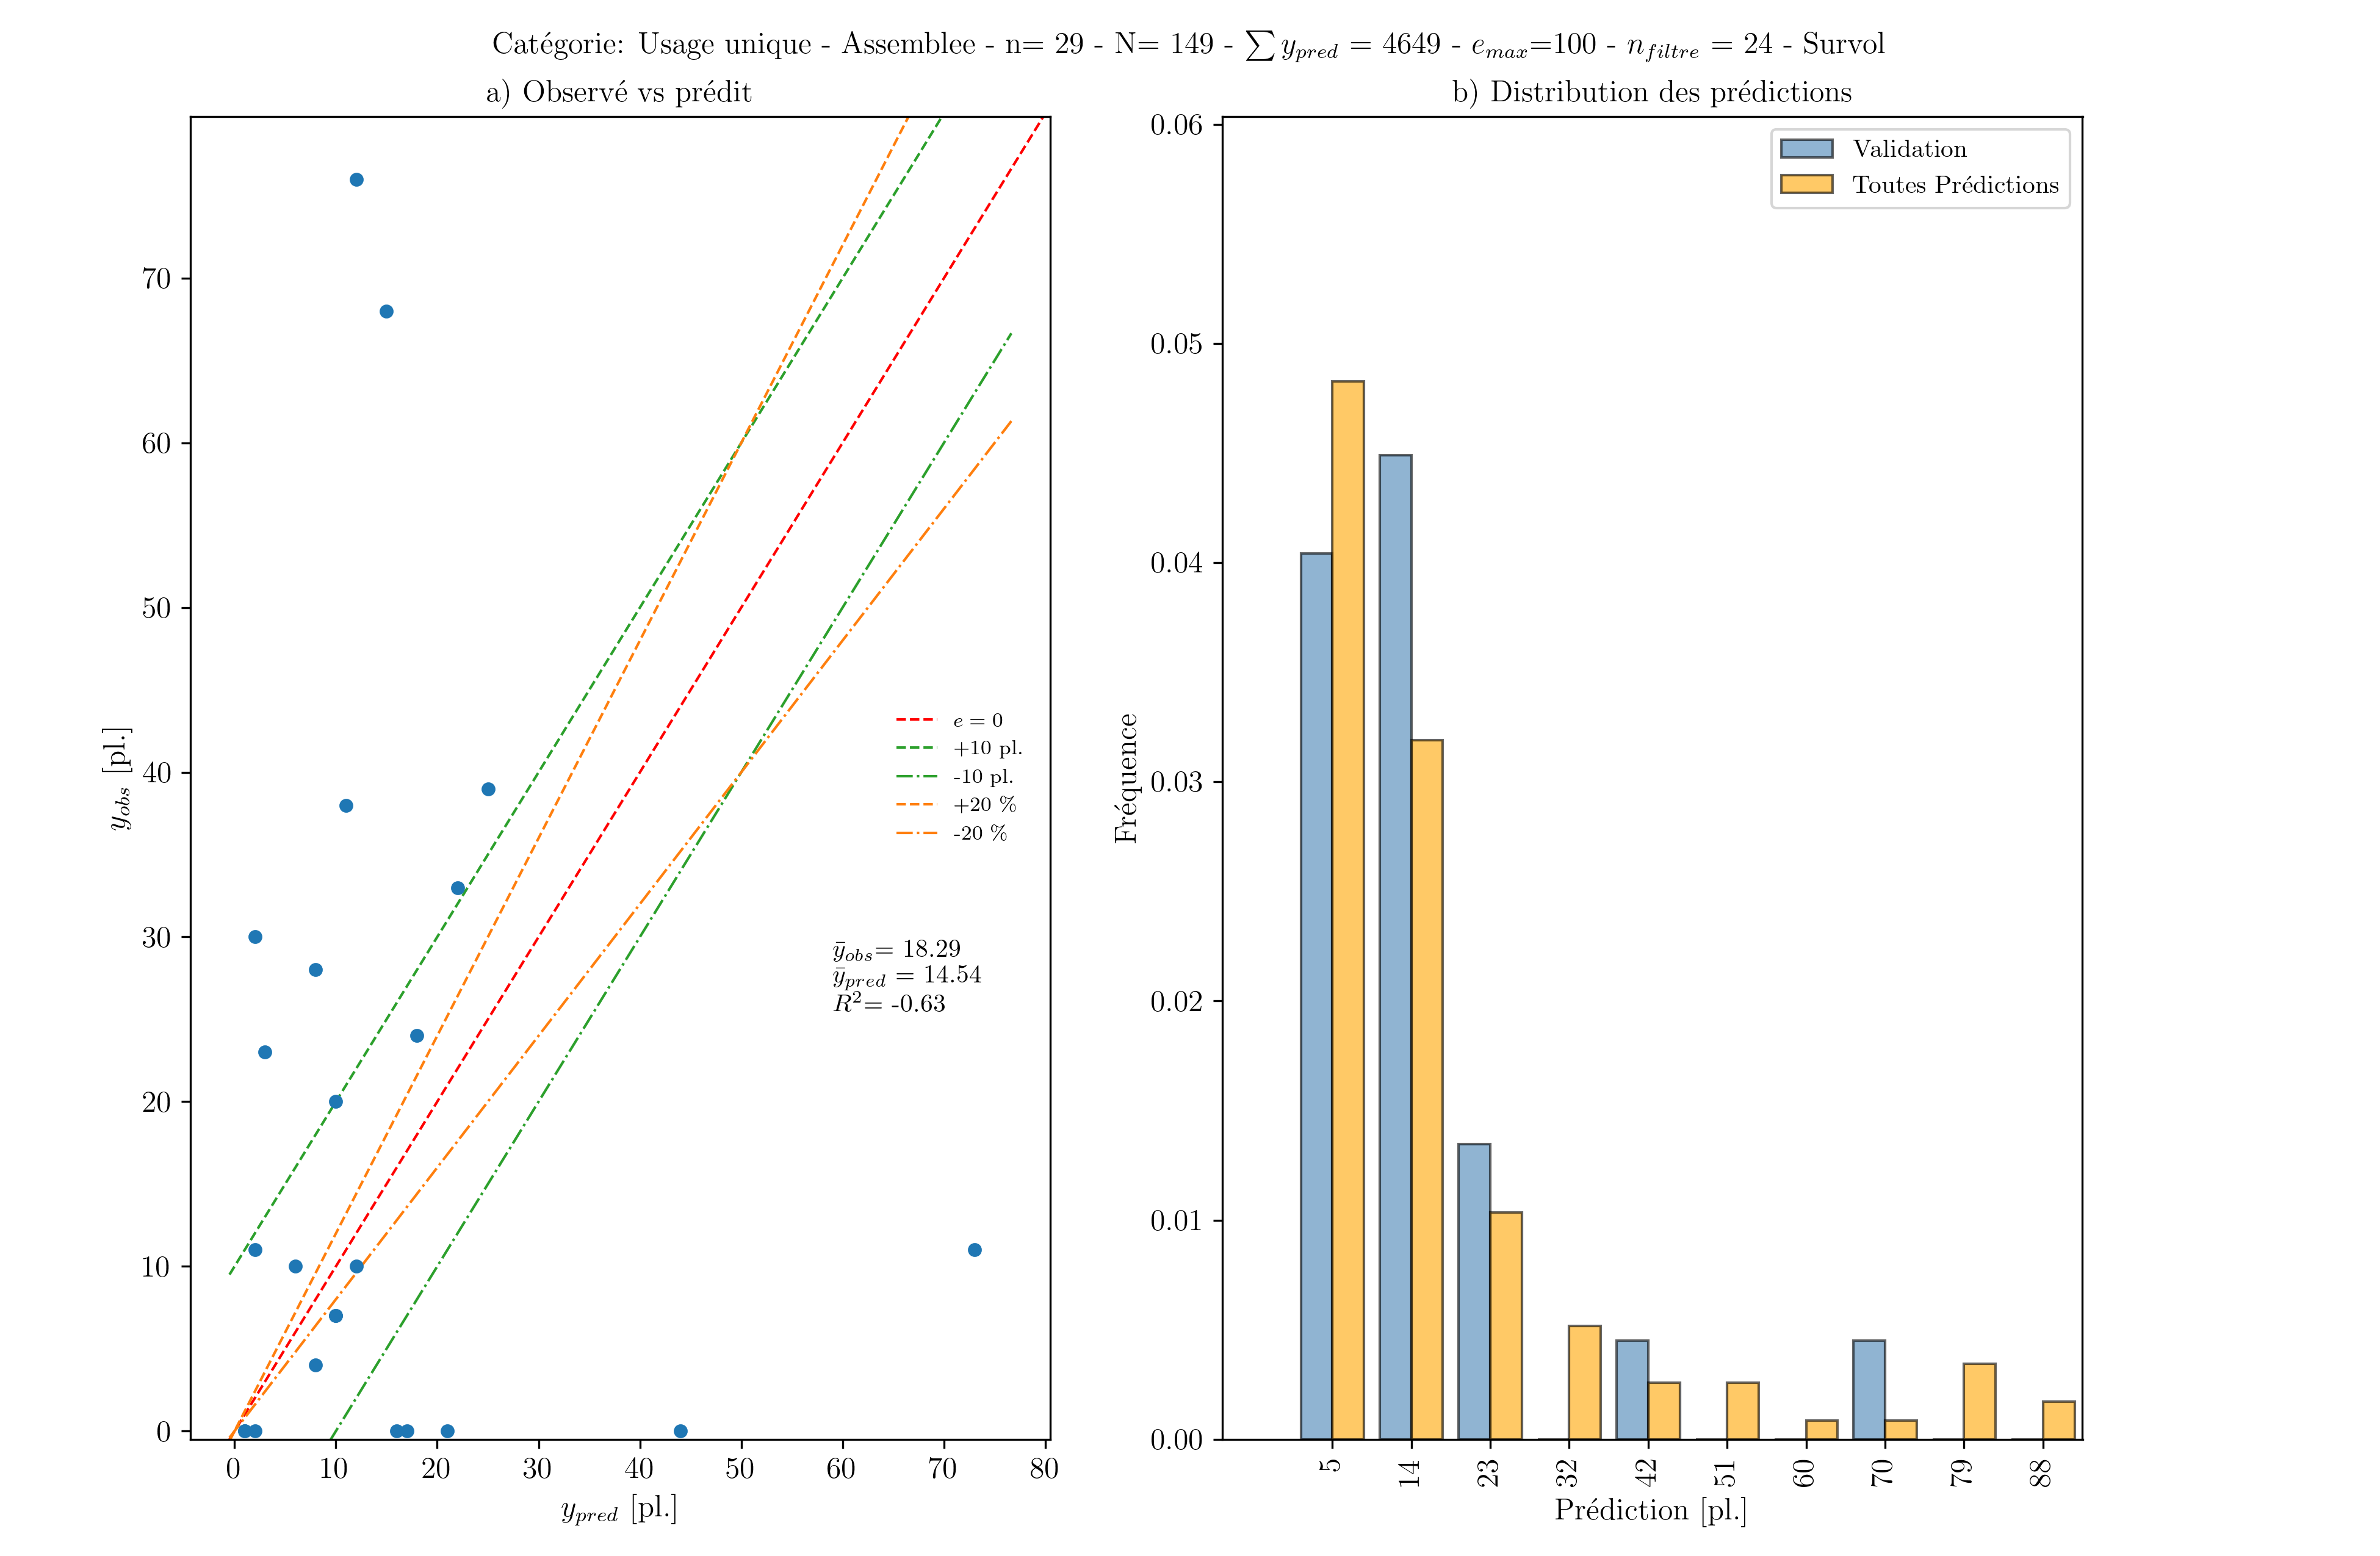
\includegraphics[width=1\linewidth]{images/int_erreur_42_e_100_se_10_pe_20_a.png}
        \caption{Distribution des prédictions pour les lots d'assemblée}
        \label{fig:int-dist-pred-ass}
    \end{figure}
    \begin{figure}[H]
        \centering
        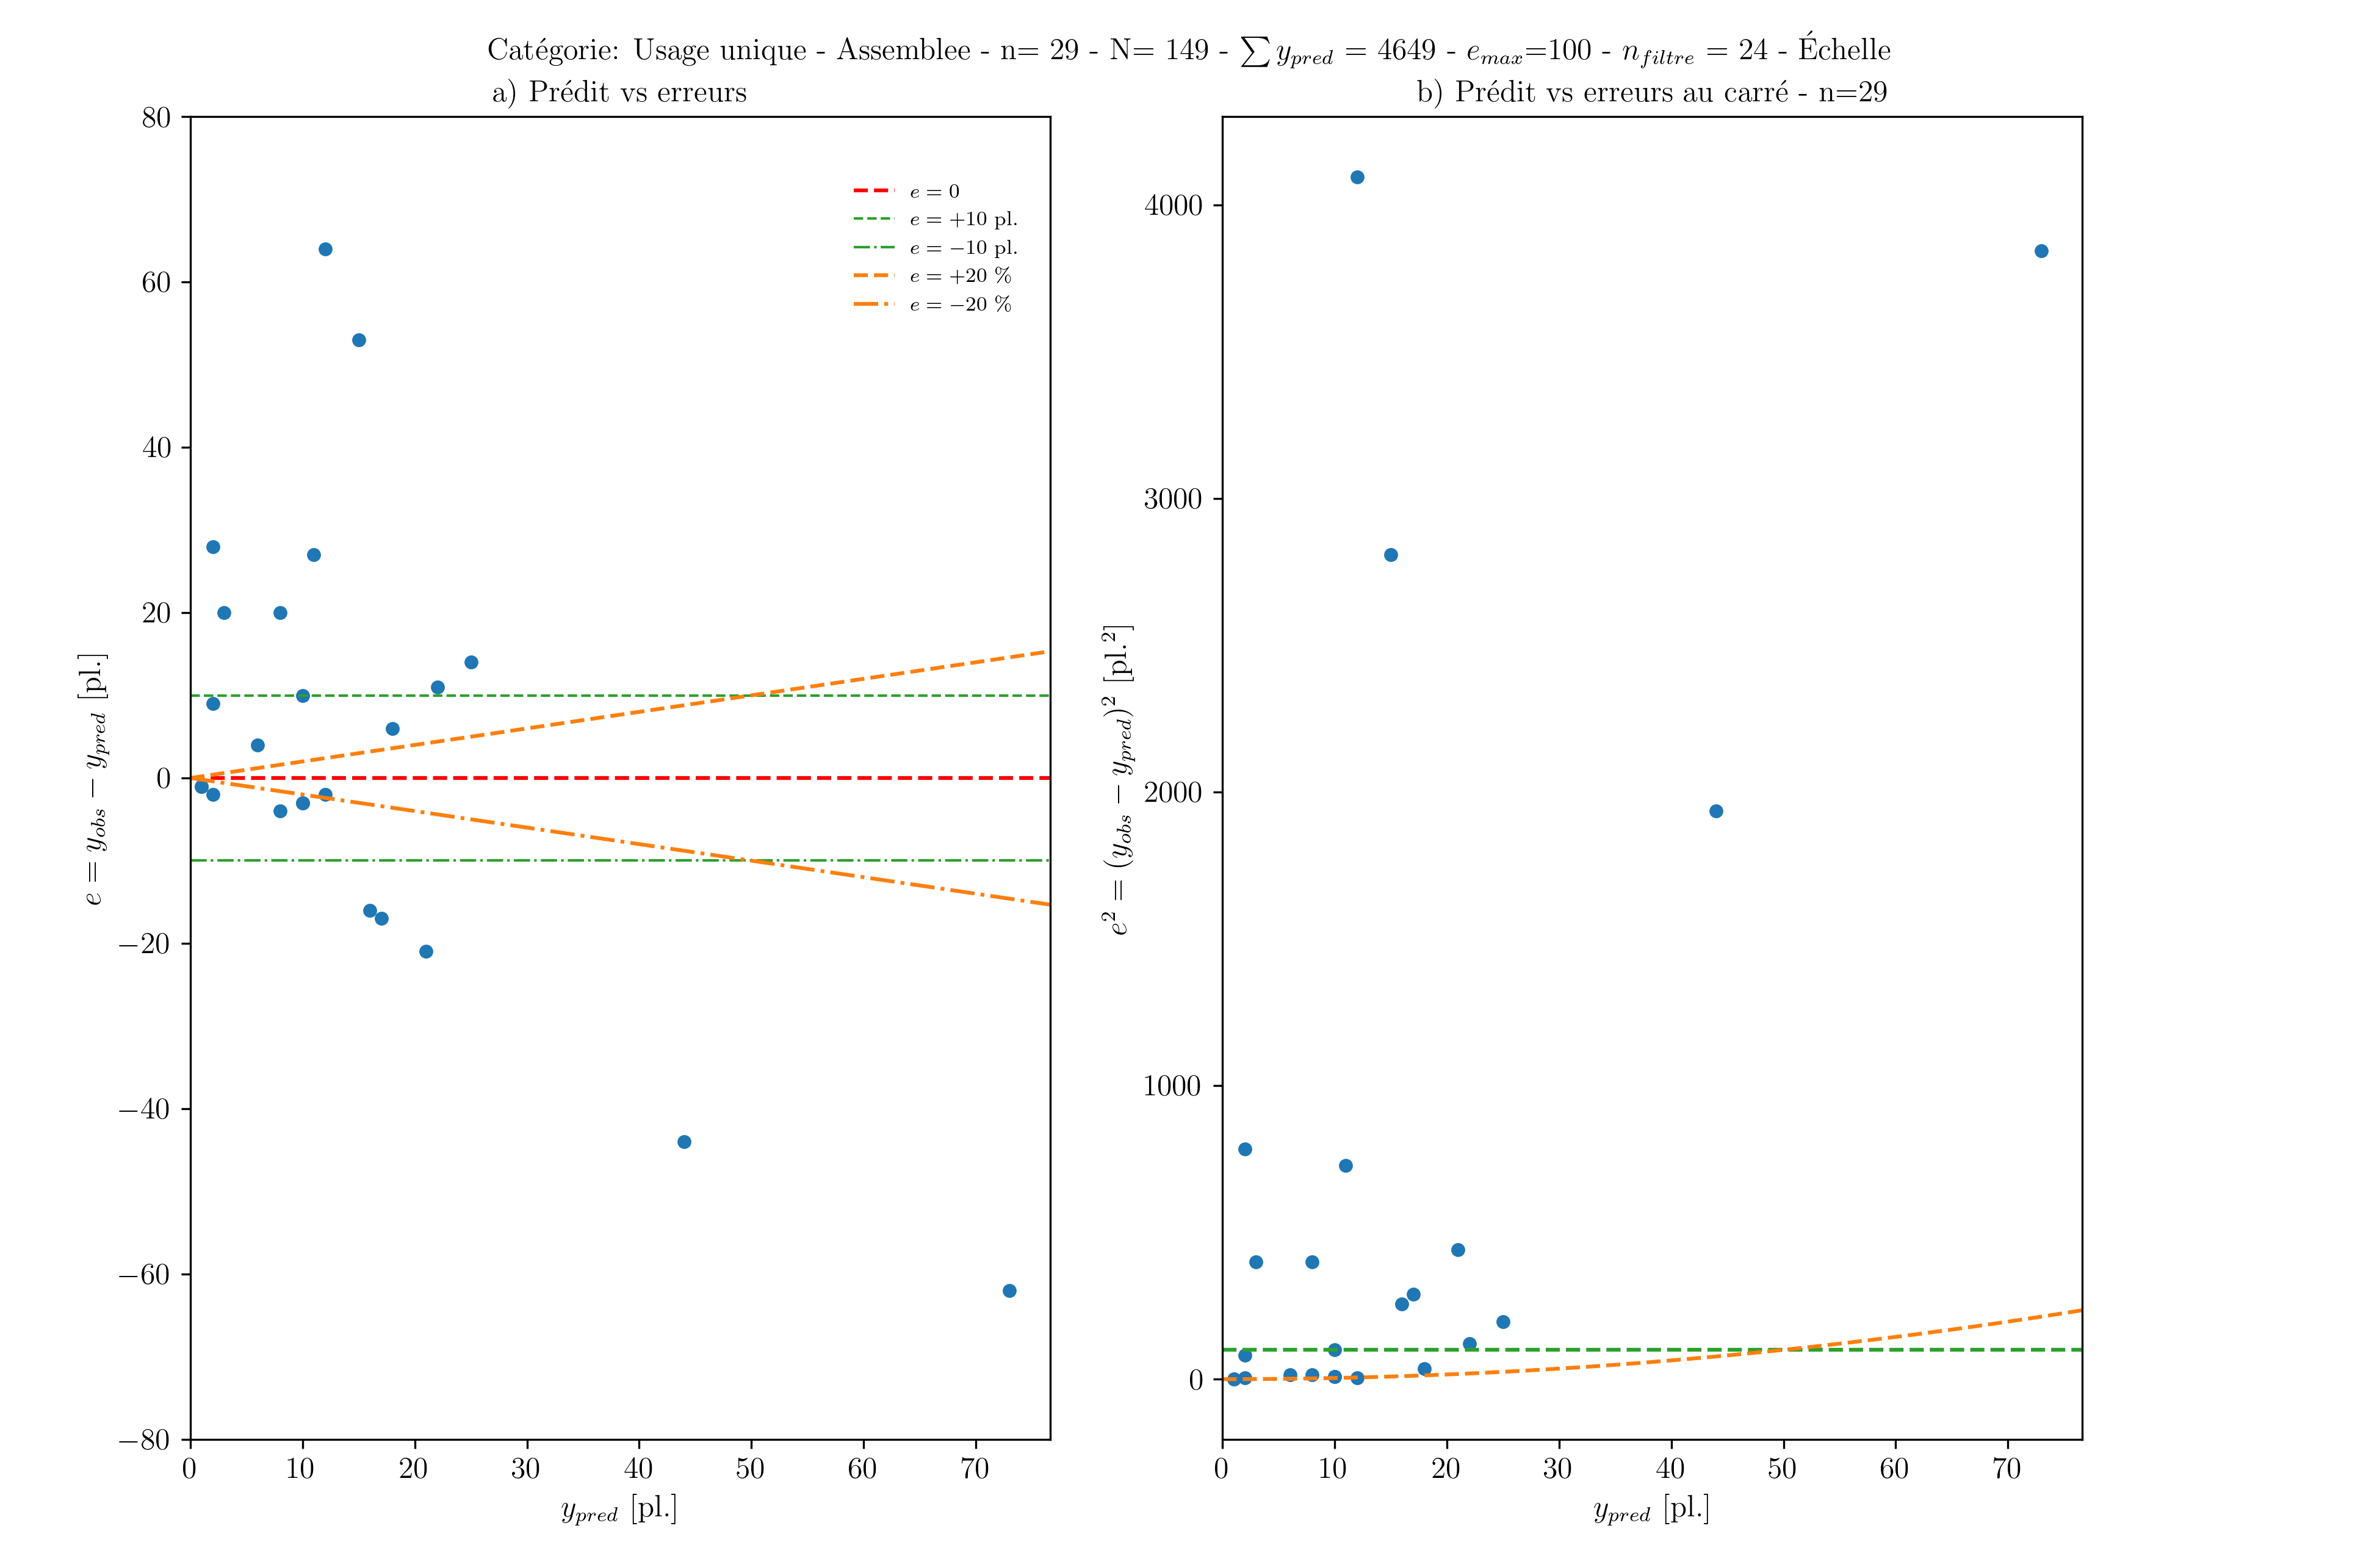
\includegraphics[width=1\linewidth]{images/int_erreur_42_e_100_se_10_pe_20_b.png}
        \caption{Erreur en fonction des prédictions pour les lots d'assemblée}
        \label{fig:err-err-quad-pred-ass}
    \end{figure}
    \begin{figure}[H]
        \centering
        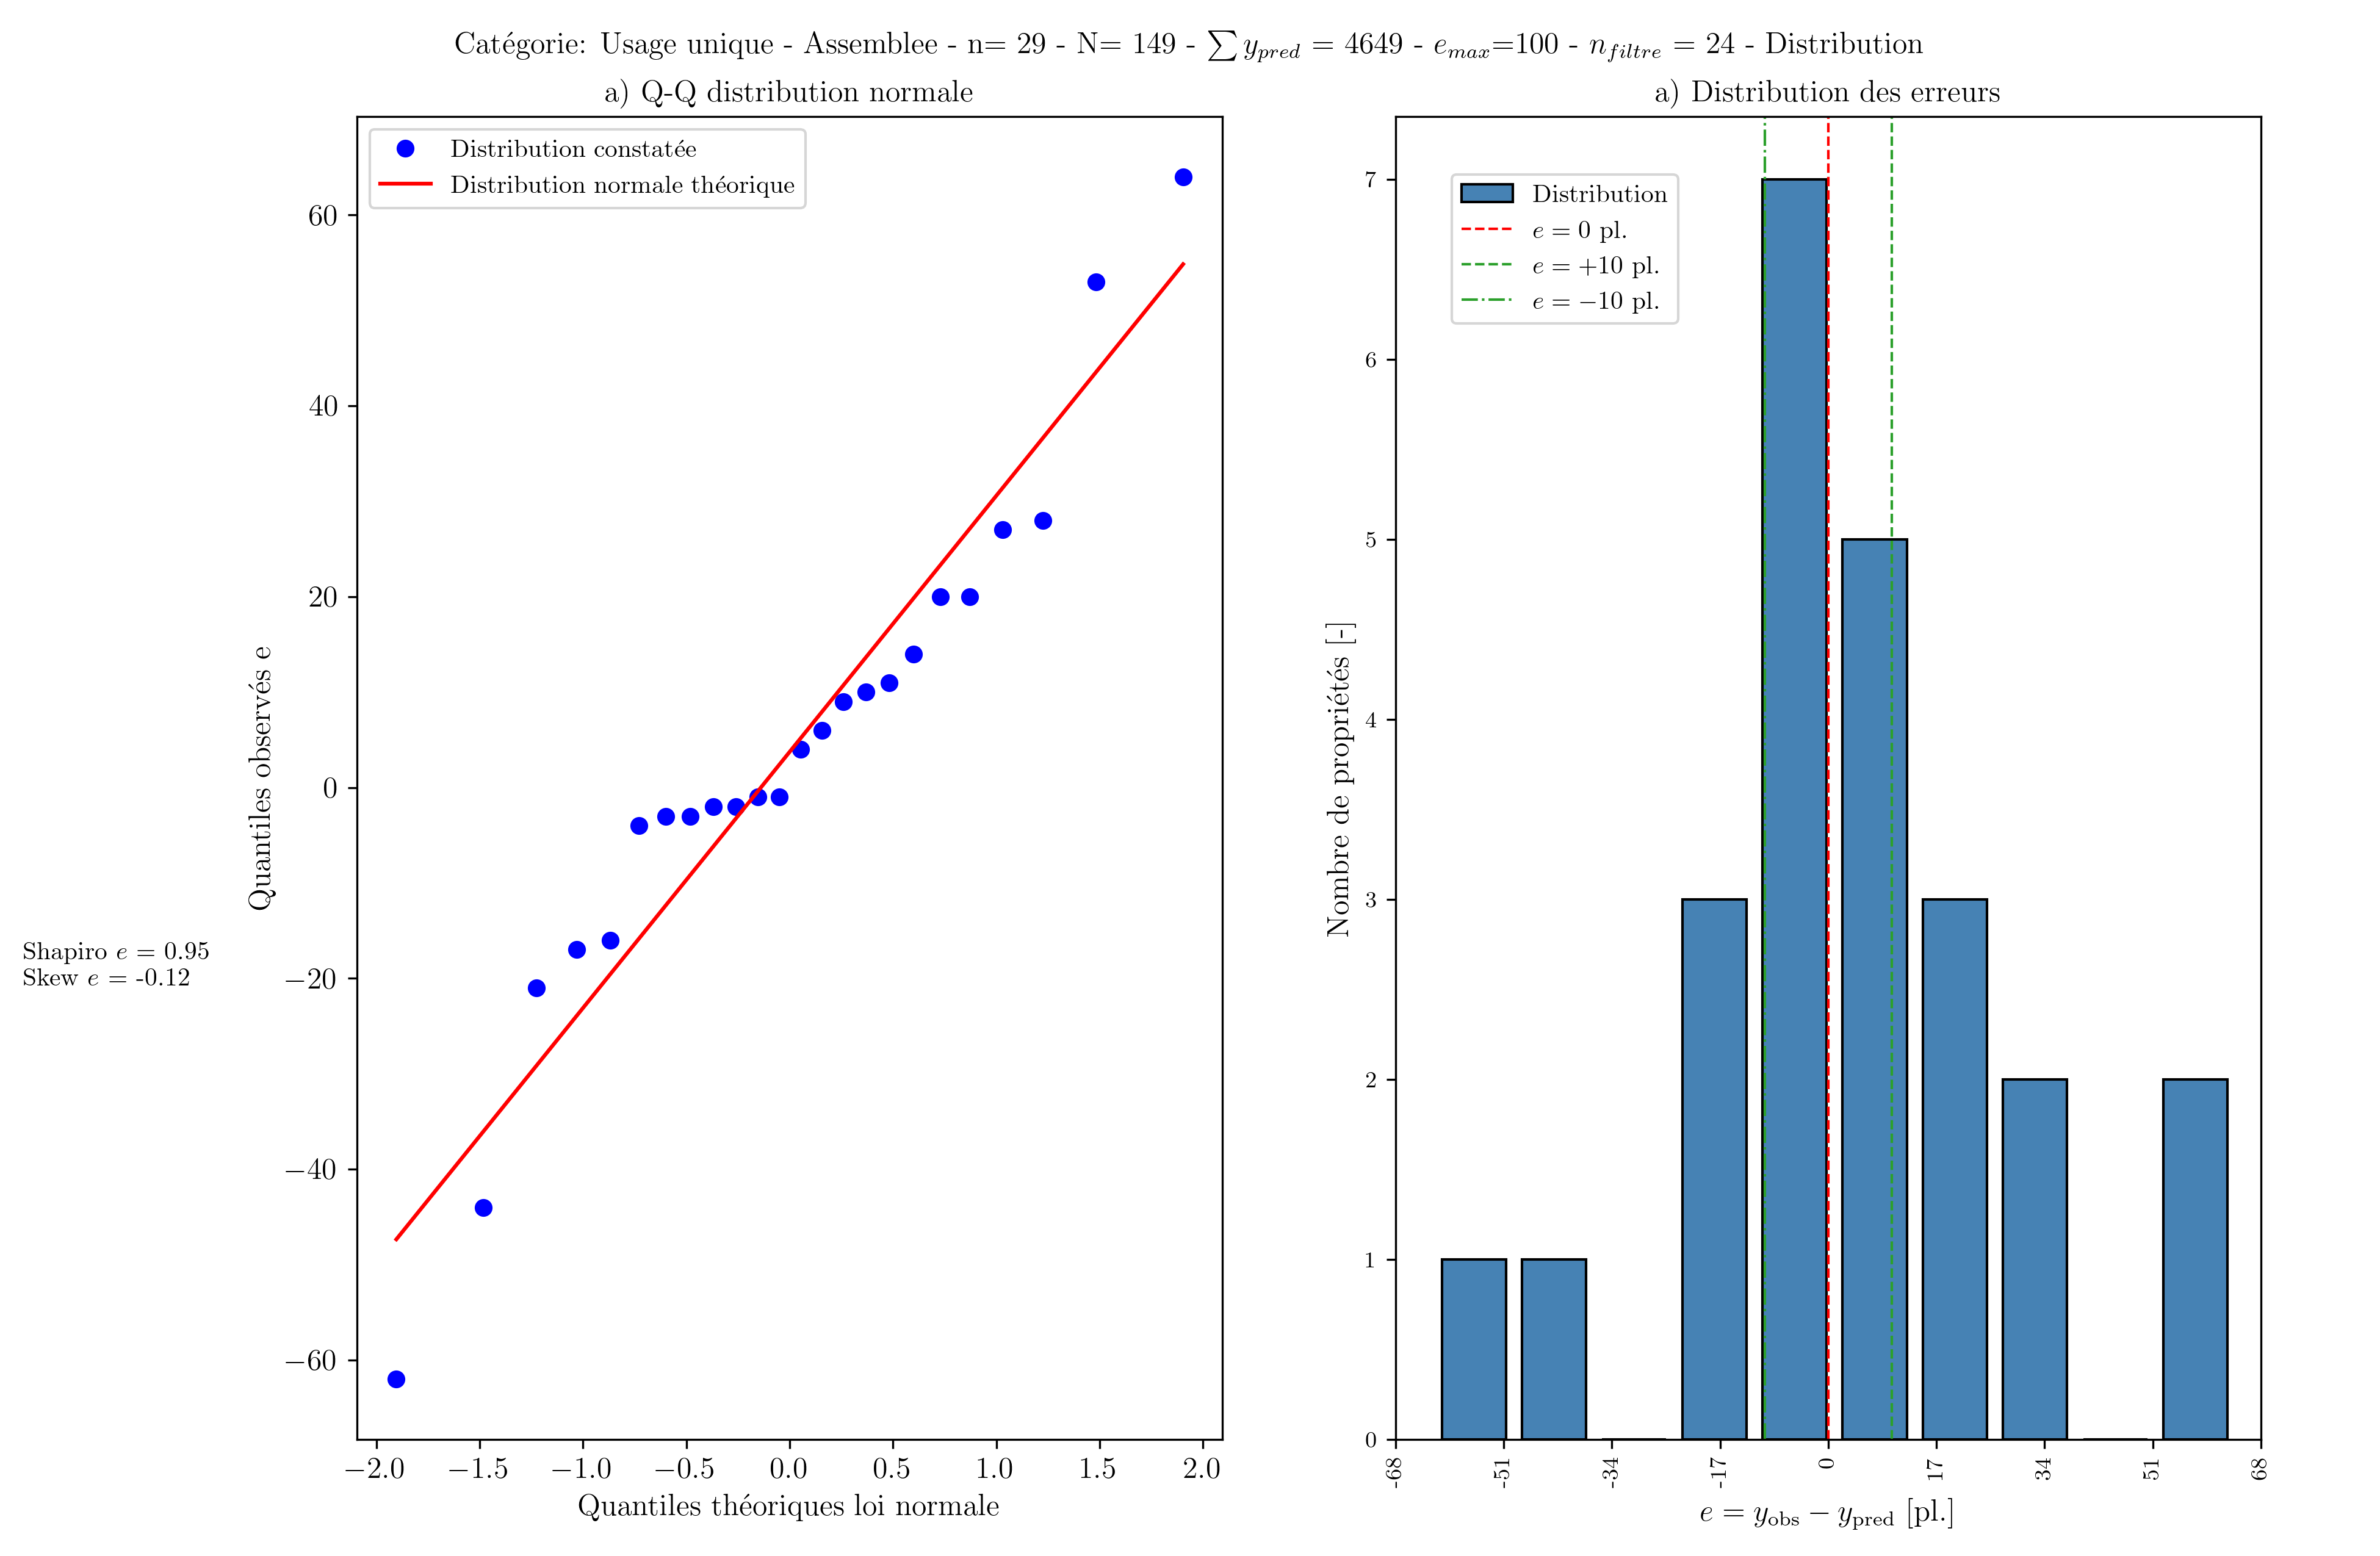
\includegraphics[width=1\linewidth]{images/int_erreur_42_e_100_se_10_pe_20_c.png}
        \caption{Distribution et normalité des erreurs pour les lots d'assemblée}
        \label{fig:dist-erreur-norm-ass}
    \end{figure}
    \begin{figure}[H]
        \centering
        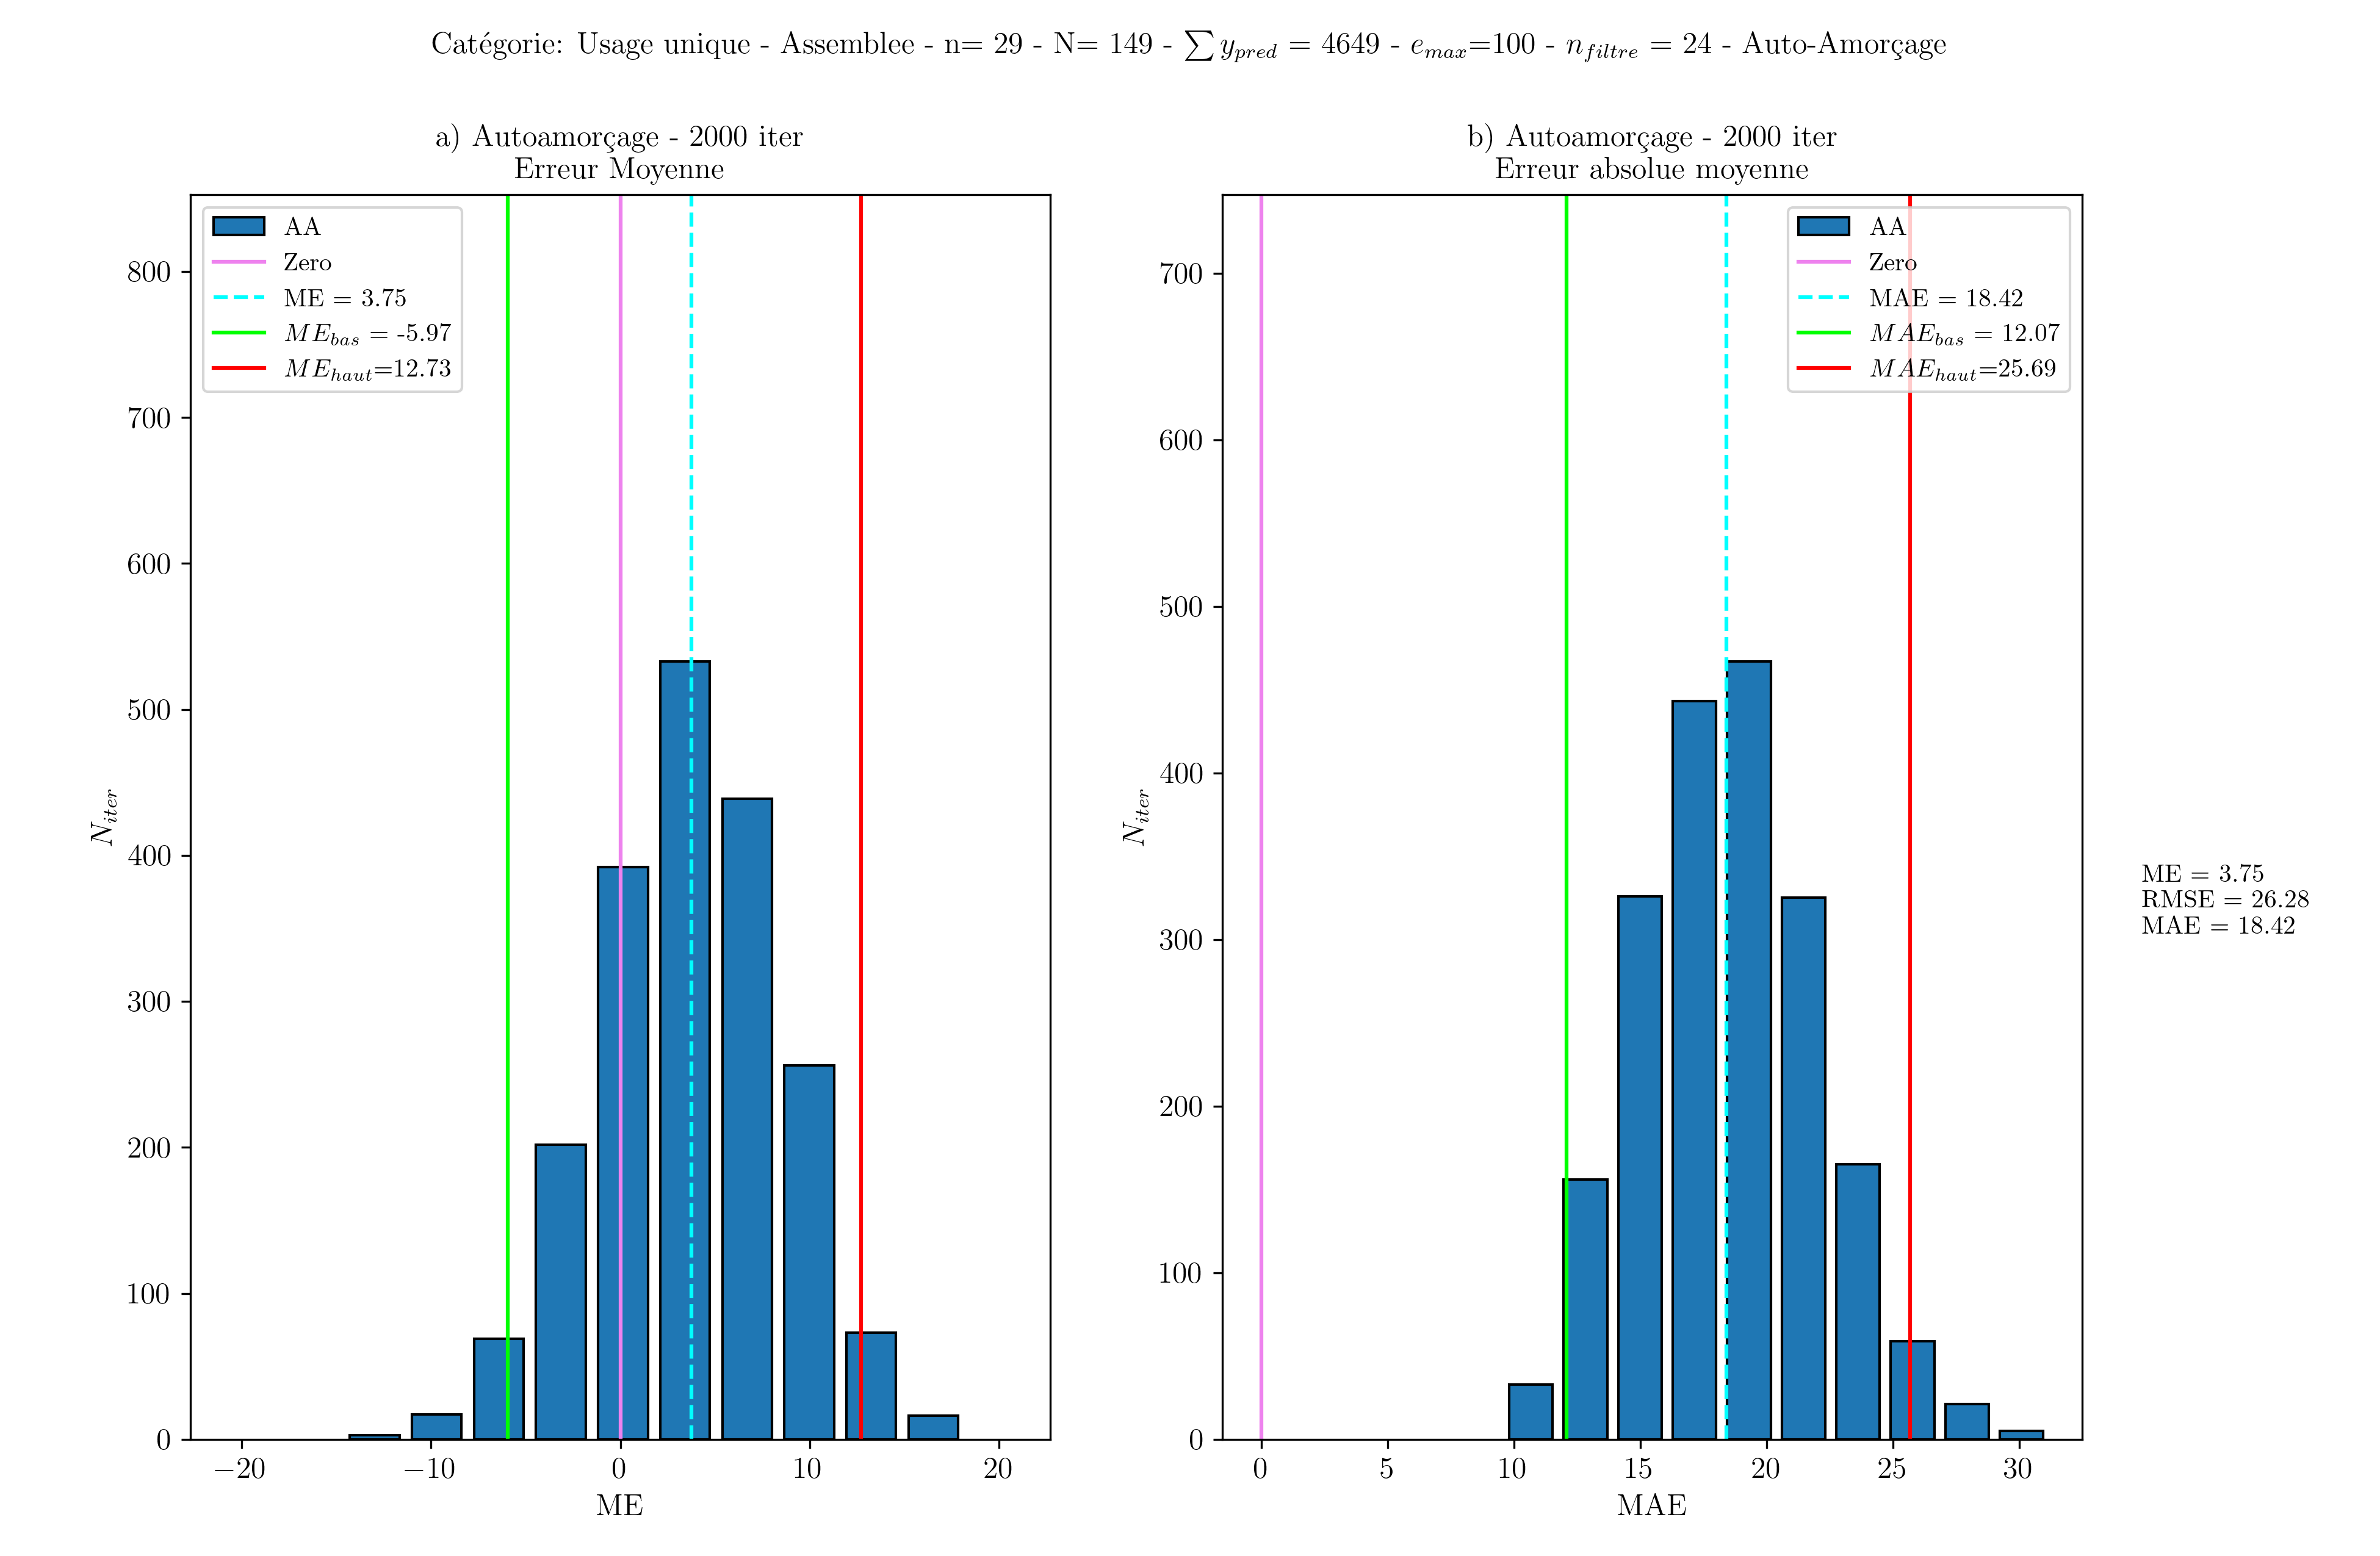
\includegraphics[width=1\linewidth]{images/int_erreur_42_e_100_se_10_pe_20_d.png}
        \caption{Distribution des métriques d'erreur après auto-amorçage pour les lots d'assemblée}
        \label{fig:auto-amor-ass}
    \end{figure}
    %\begin{figure}
    %    \centering
    %    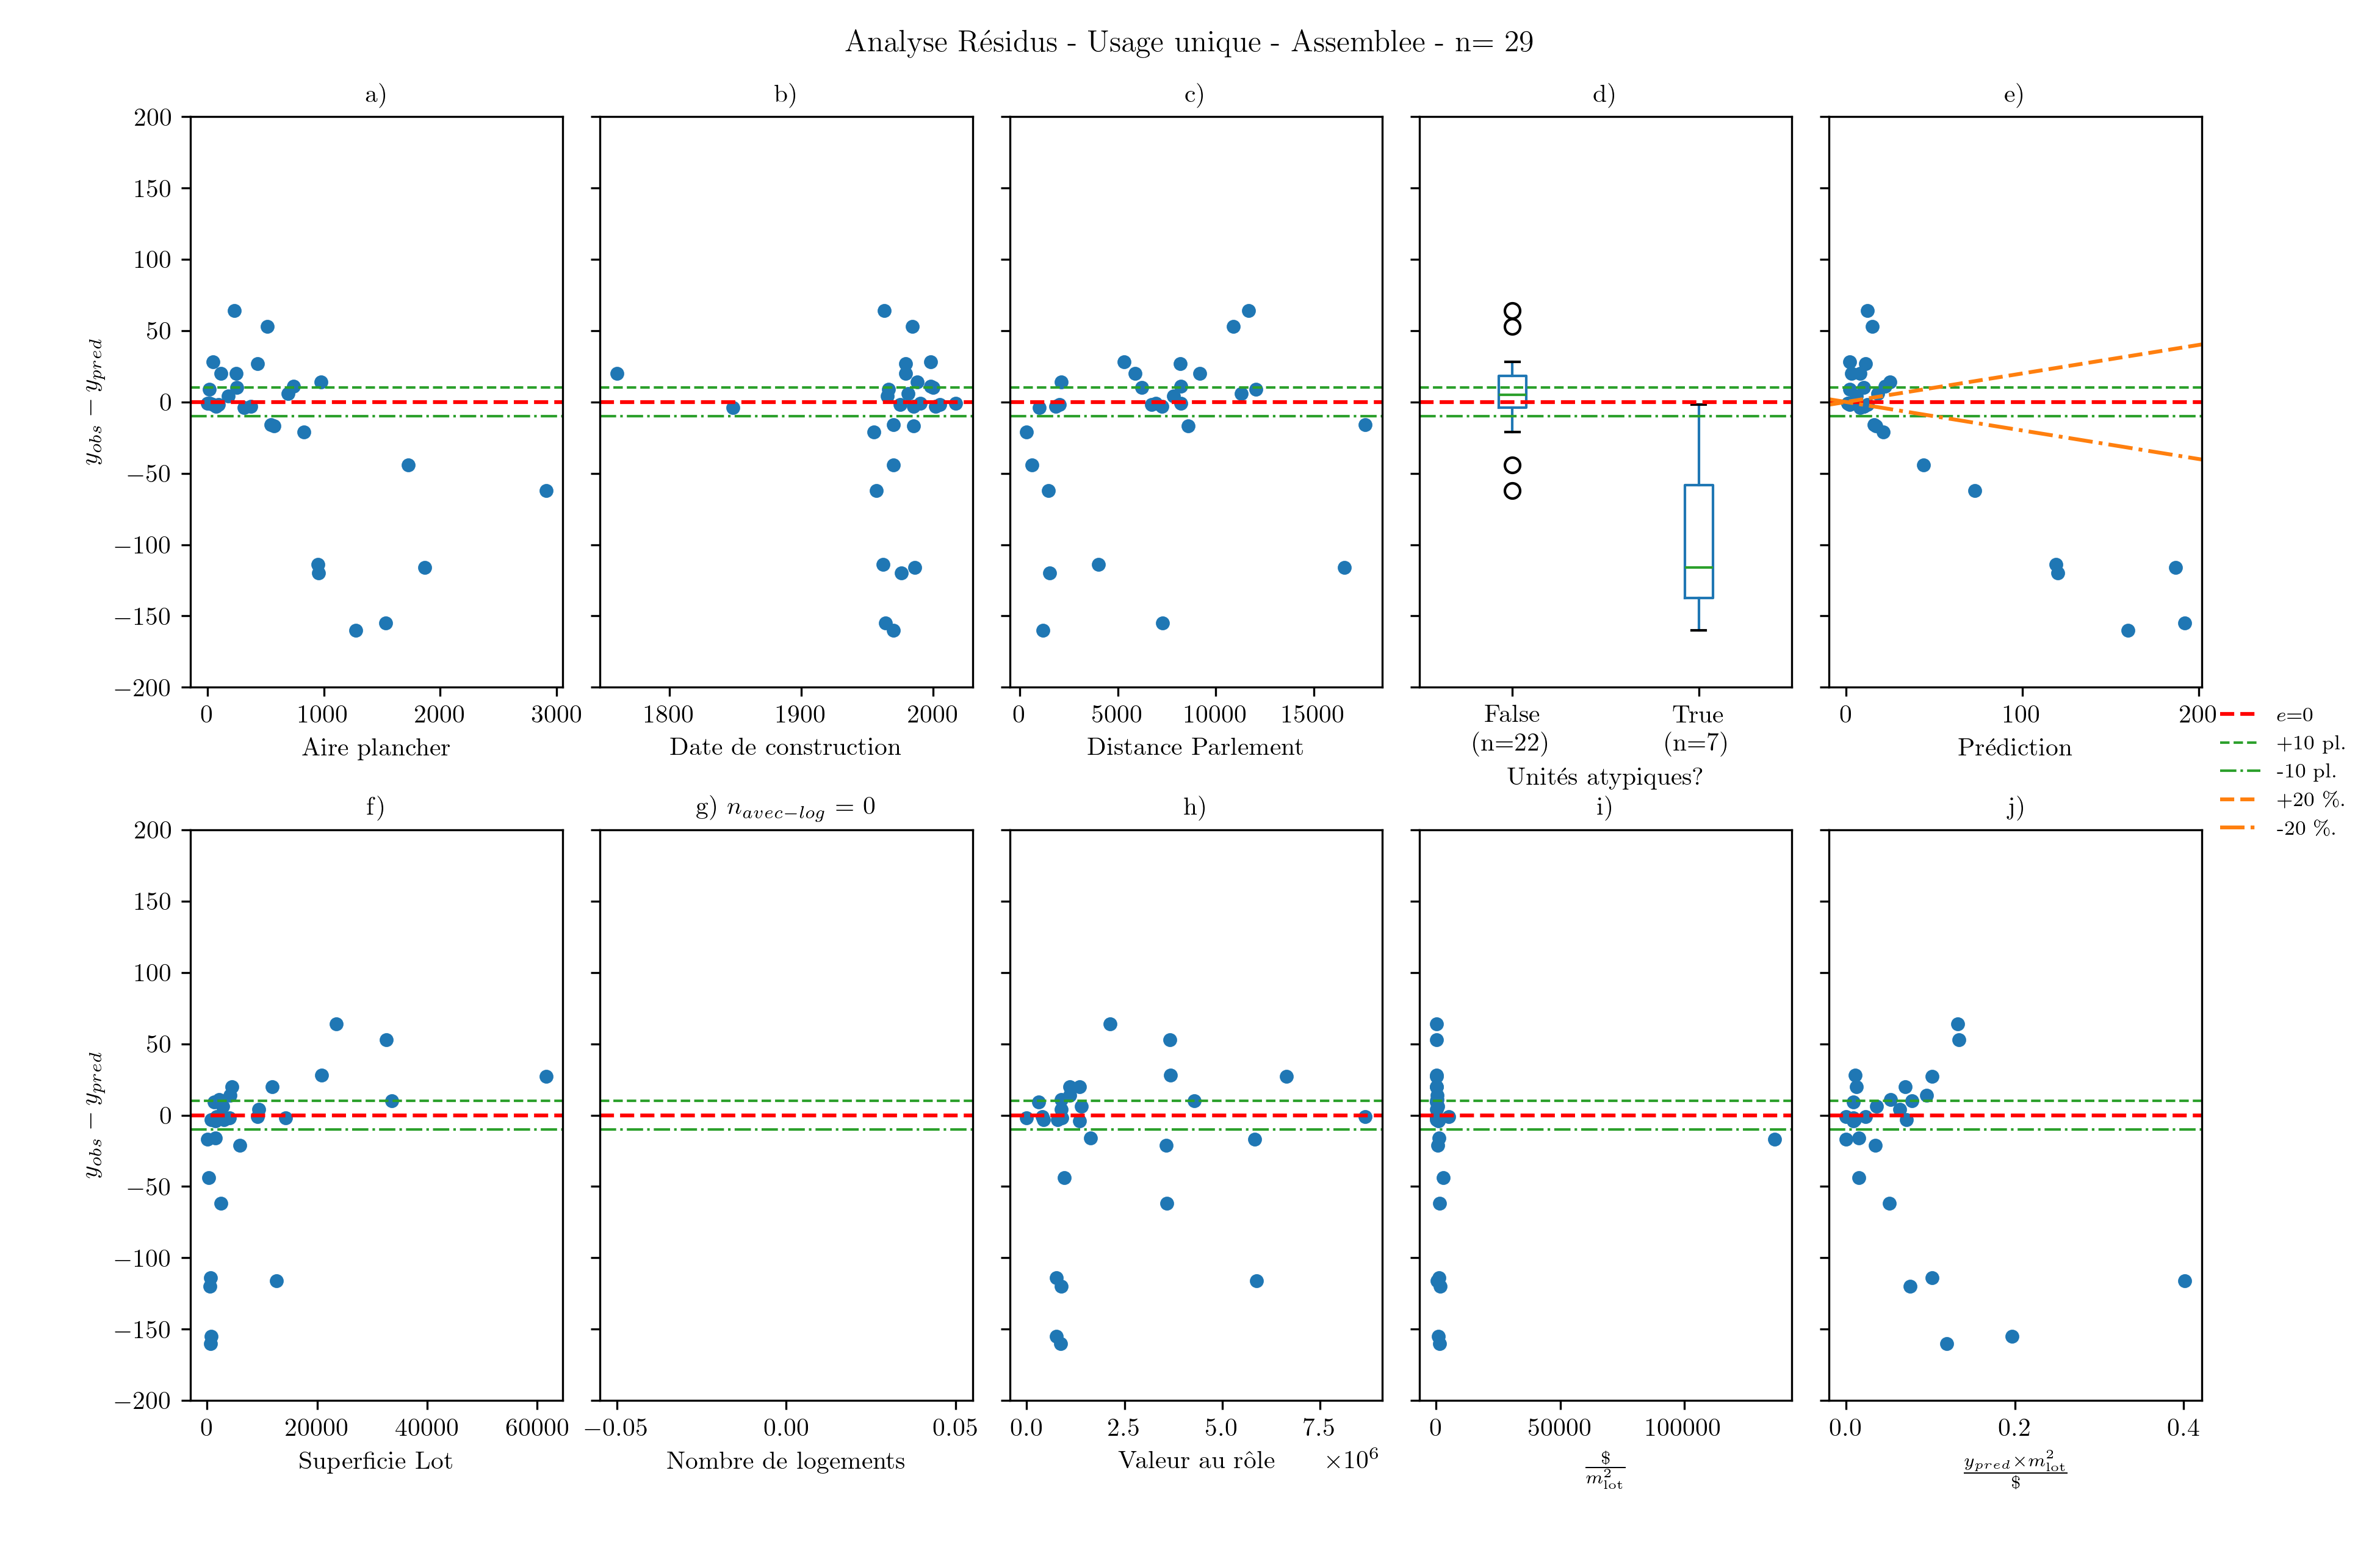
\includegraphics[scale=0.65]{images/ana_res_42_se_10_pe_20.png}
    %    \caption{Analyse des propriétés d'assemblée et de récréation sans filtre sur le nombre de places}
    %    \label{fig:ana-residu-assem}
    %\end{figure}
    \begin{figure}[H]
        \centering
        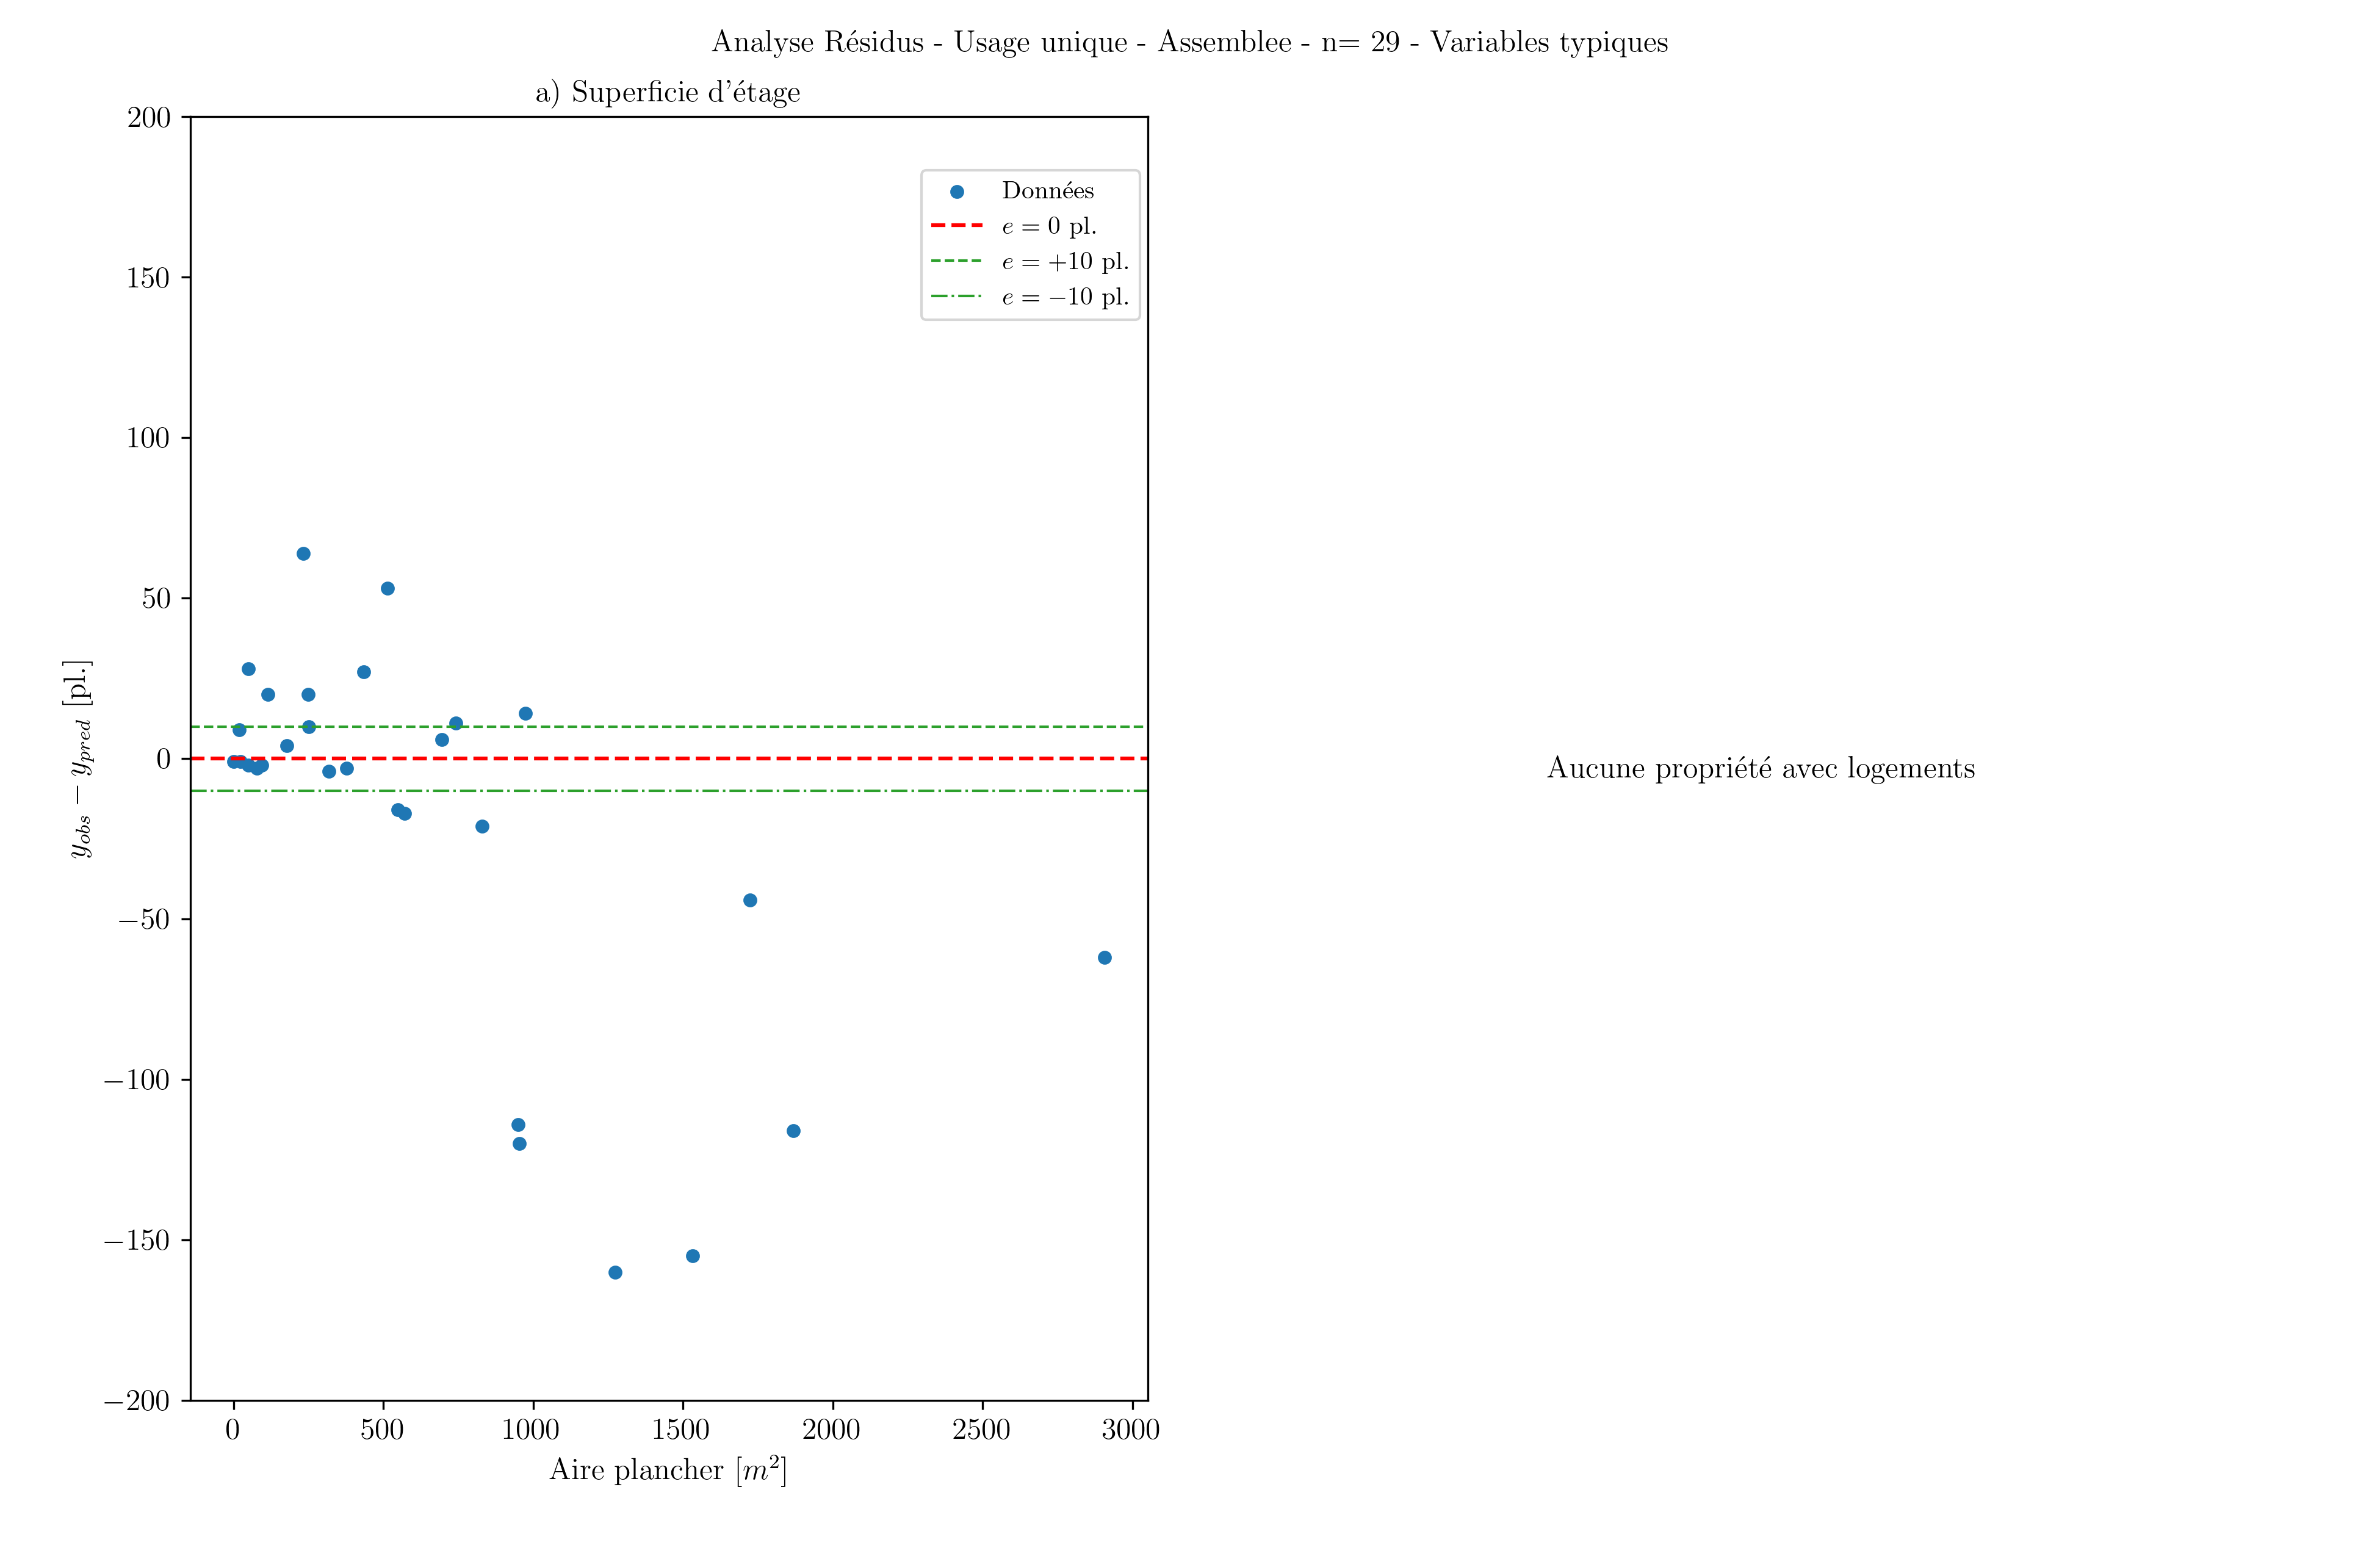
\includegraphics[width=1\linewidth]{images/ana_res_42_se_10_pe_20_a.png}
        \caption{Analyse des résidus en fonction des propriétés de construction pour les lots d'assemblée}
        \label{fig:ana-res-prop-phys-ass}
    \end{figure}
    \begin{figure}[H]
        \centering
        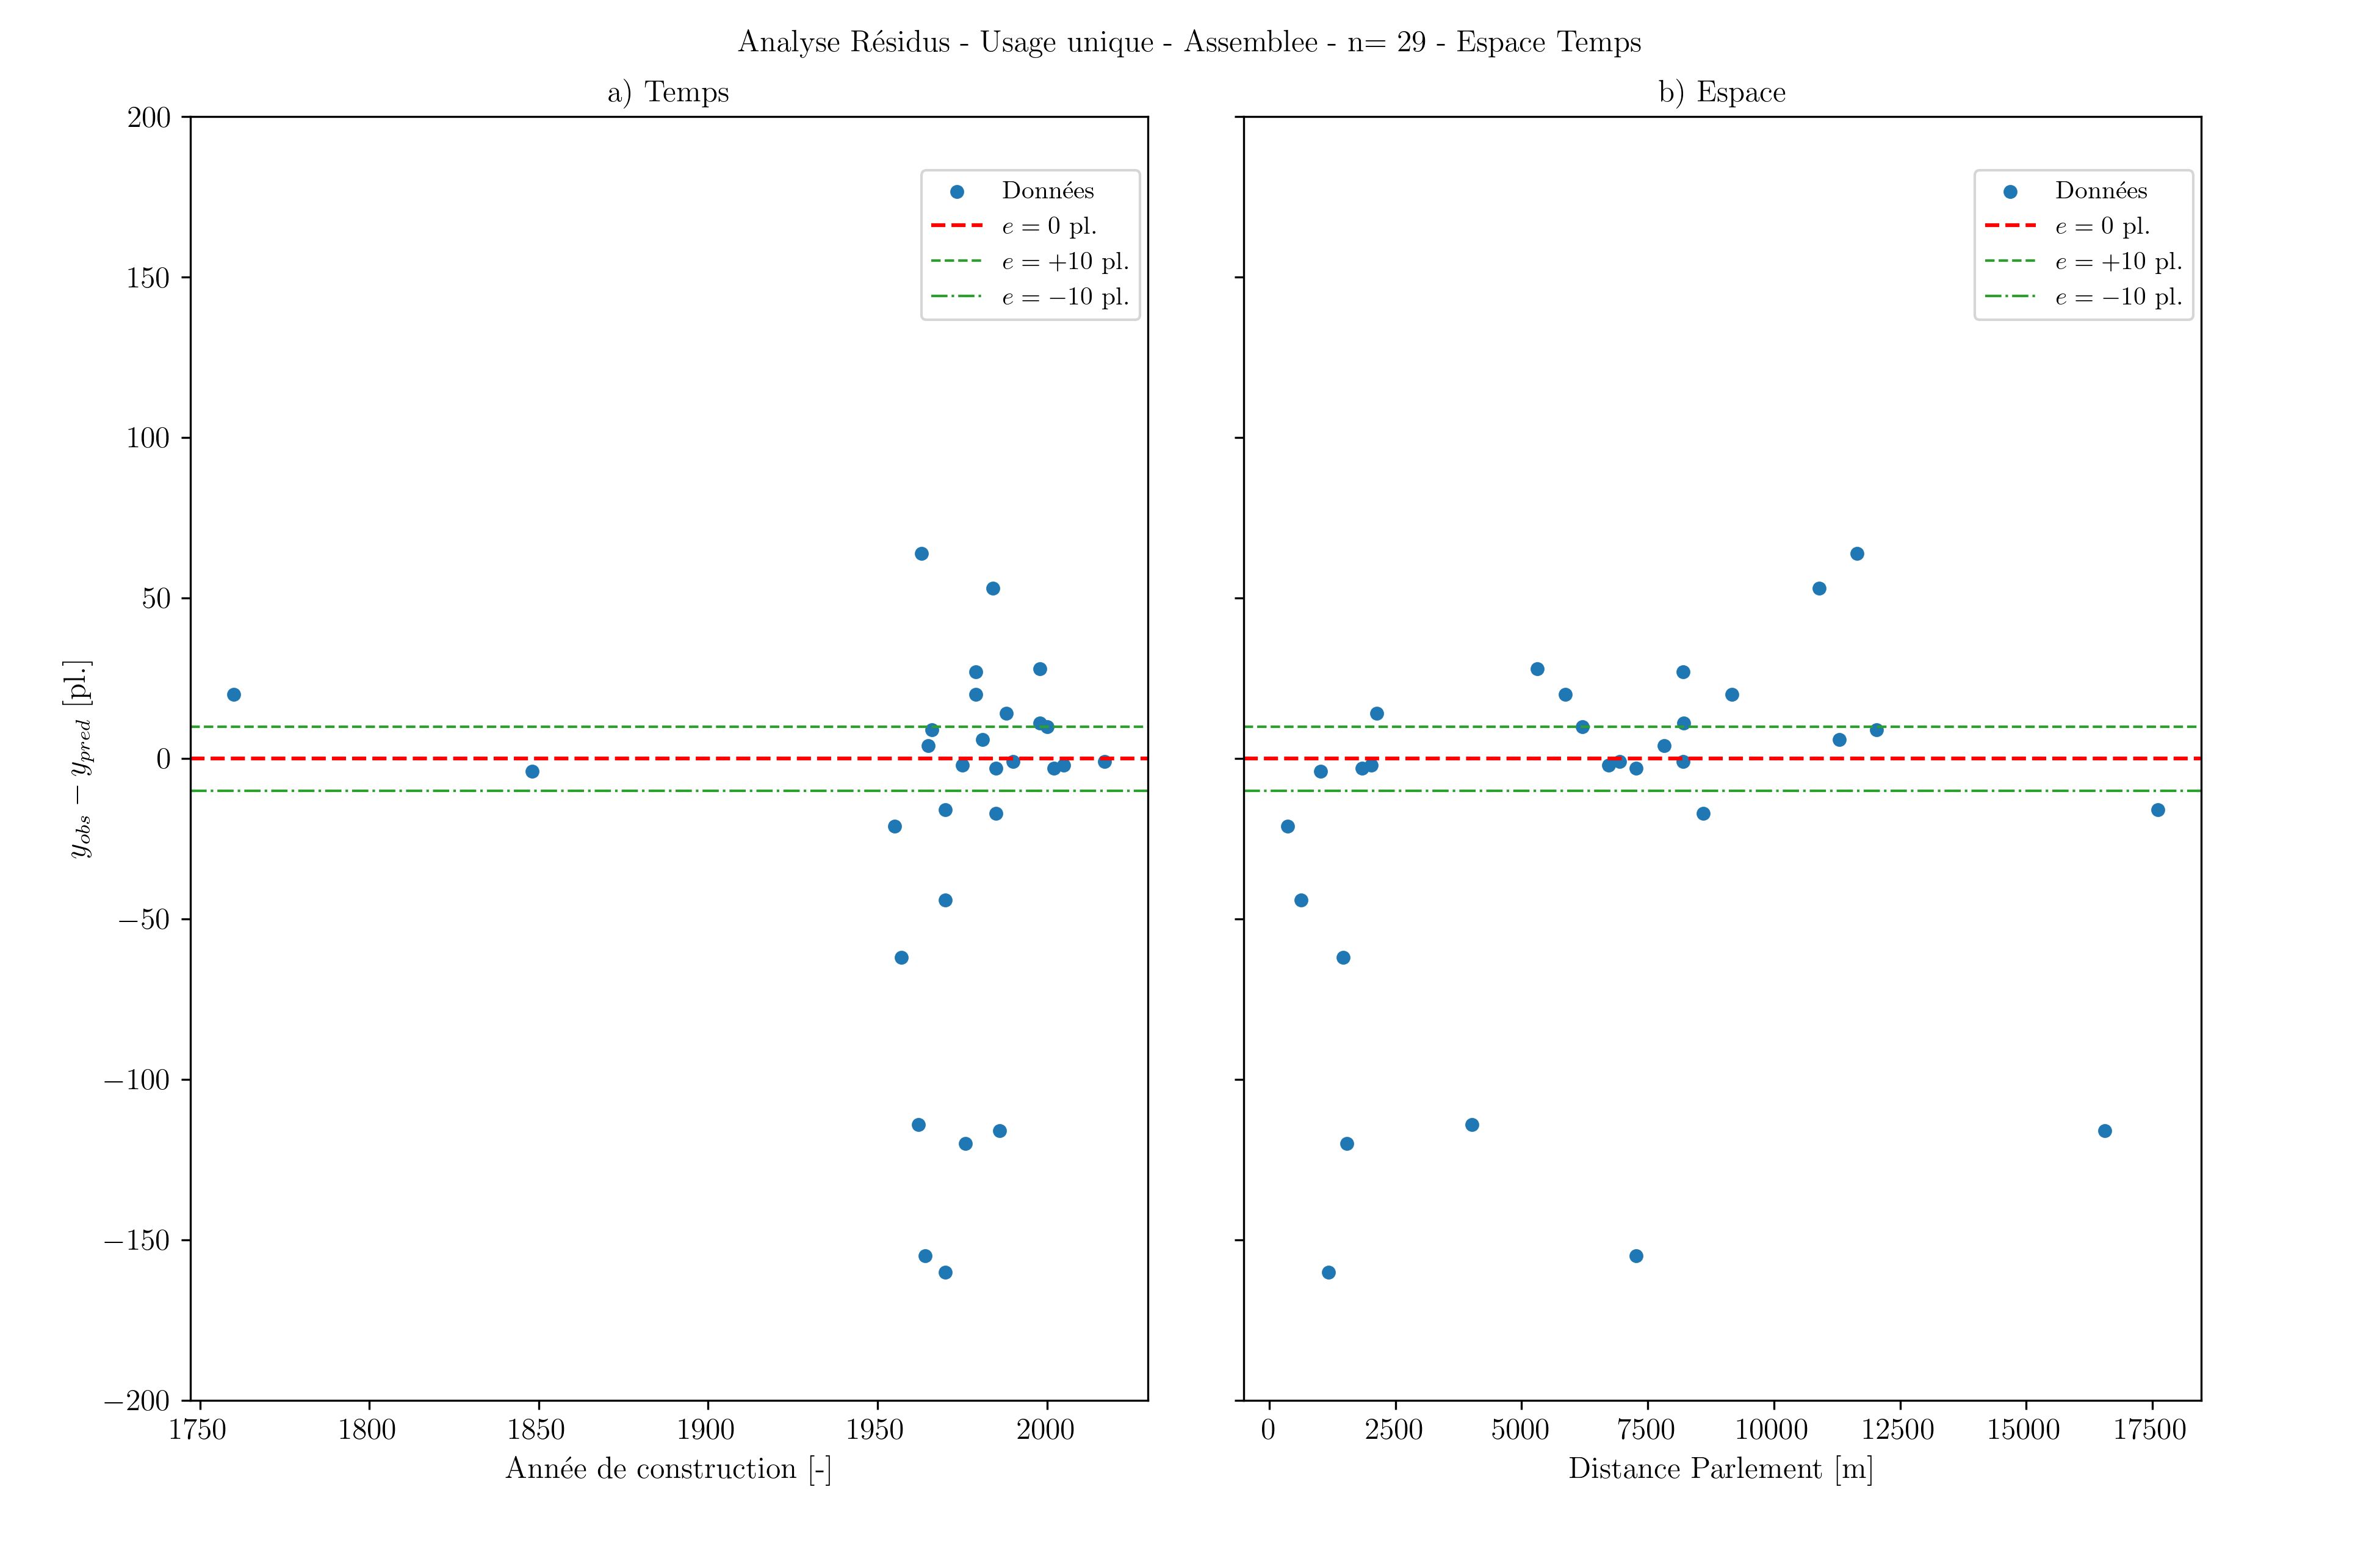
\includegraphics[width=1\linewidth]{images/ana_res_42_se_10_pe_20_b.png}
        \caption{Analyse des résidus en fonction de l'espace et de l'époque de construction pour les lots d'assemblée}
        \label{fig:ana-res-esp-temps-ass}
    \end{figure}
    \begin{figure}[H]
        \centering
        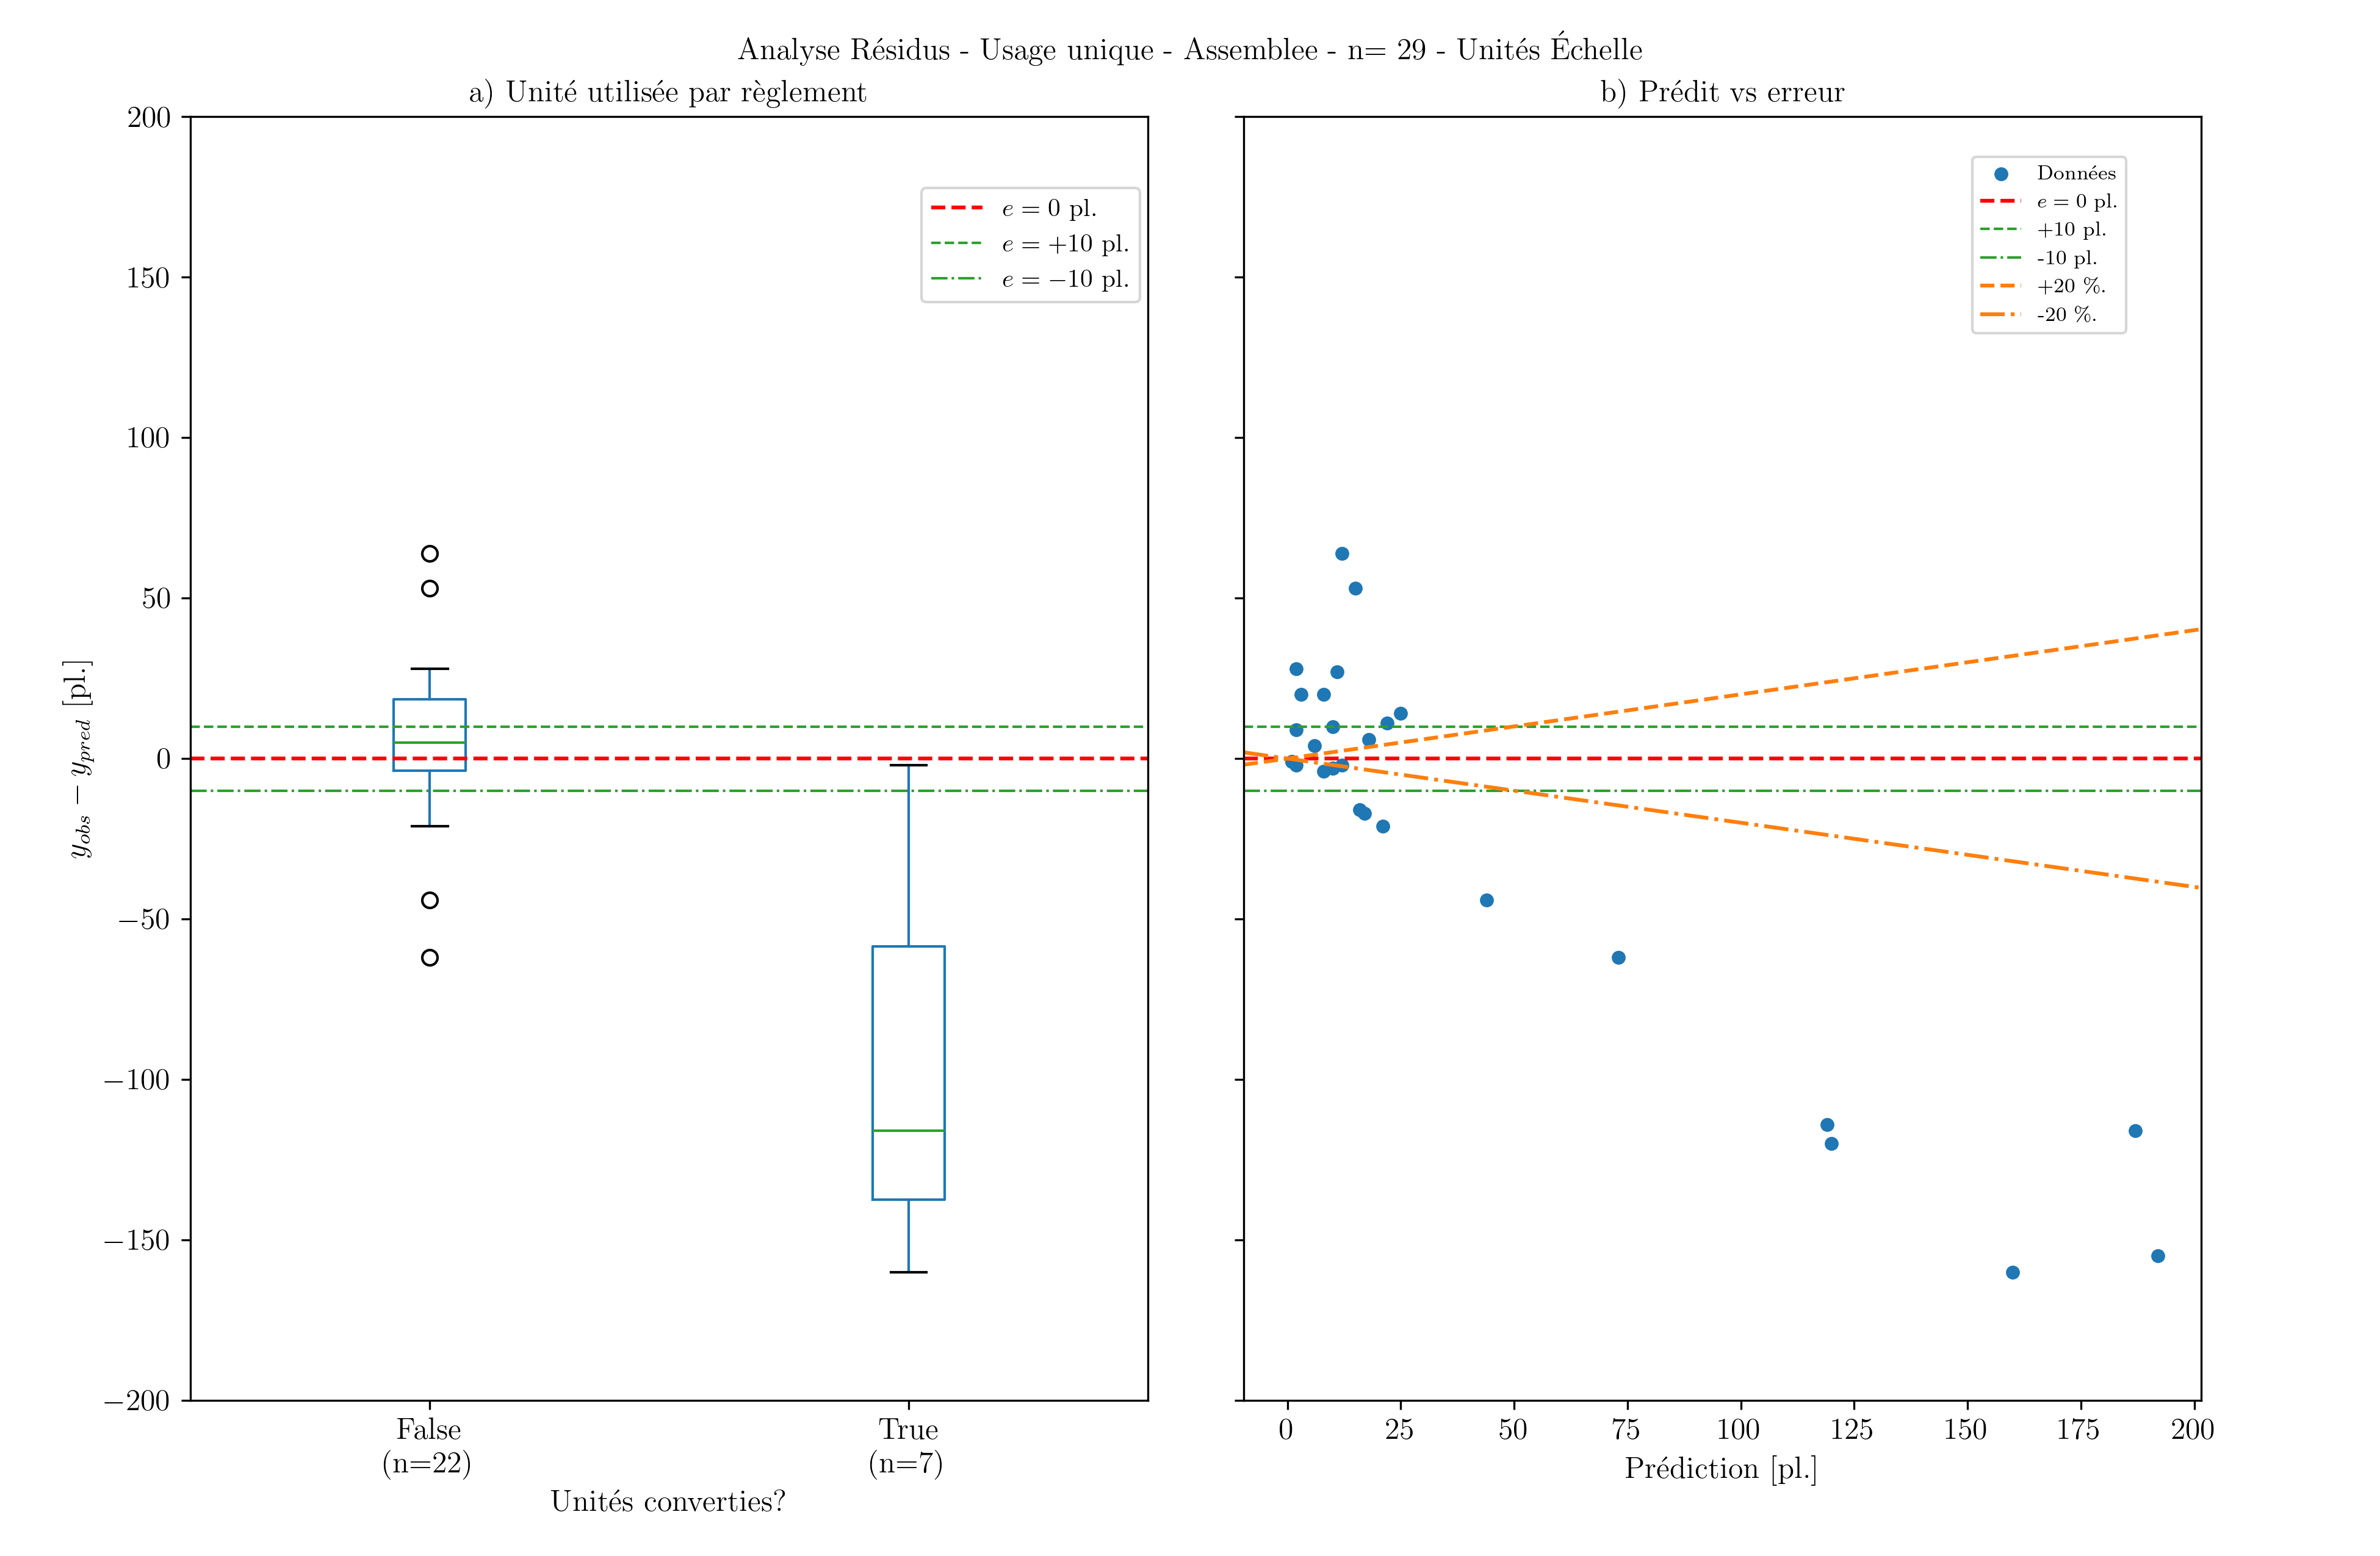
\includegraphics[width=1\linewidth]{images/ana_res_42_se_10_pe_20_c.png}
        \caption{Analyse des résidus en fonction de la prédiction et des unités de formulation pour les lots d'assemblée}
        \label{fig:ana-res-unit-pred-ass}
    \end{figure}
    \begin{figure}[H]
        \centering
        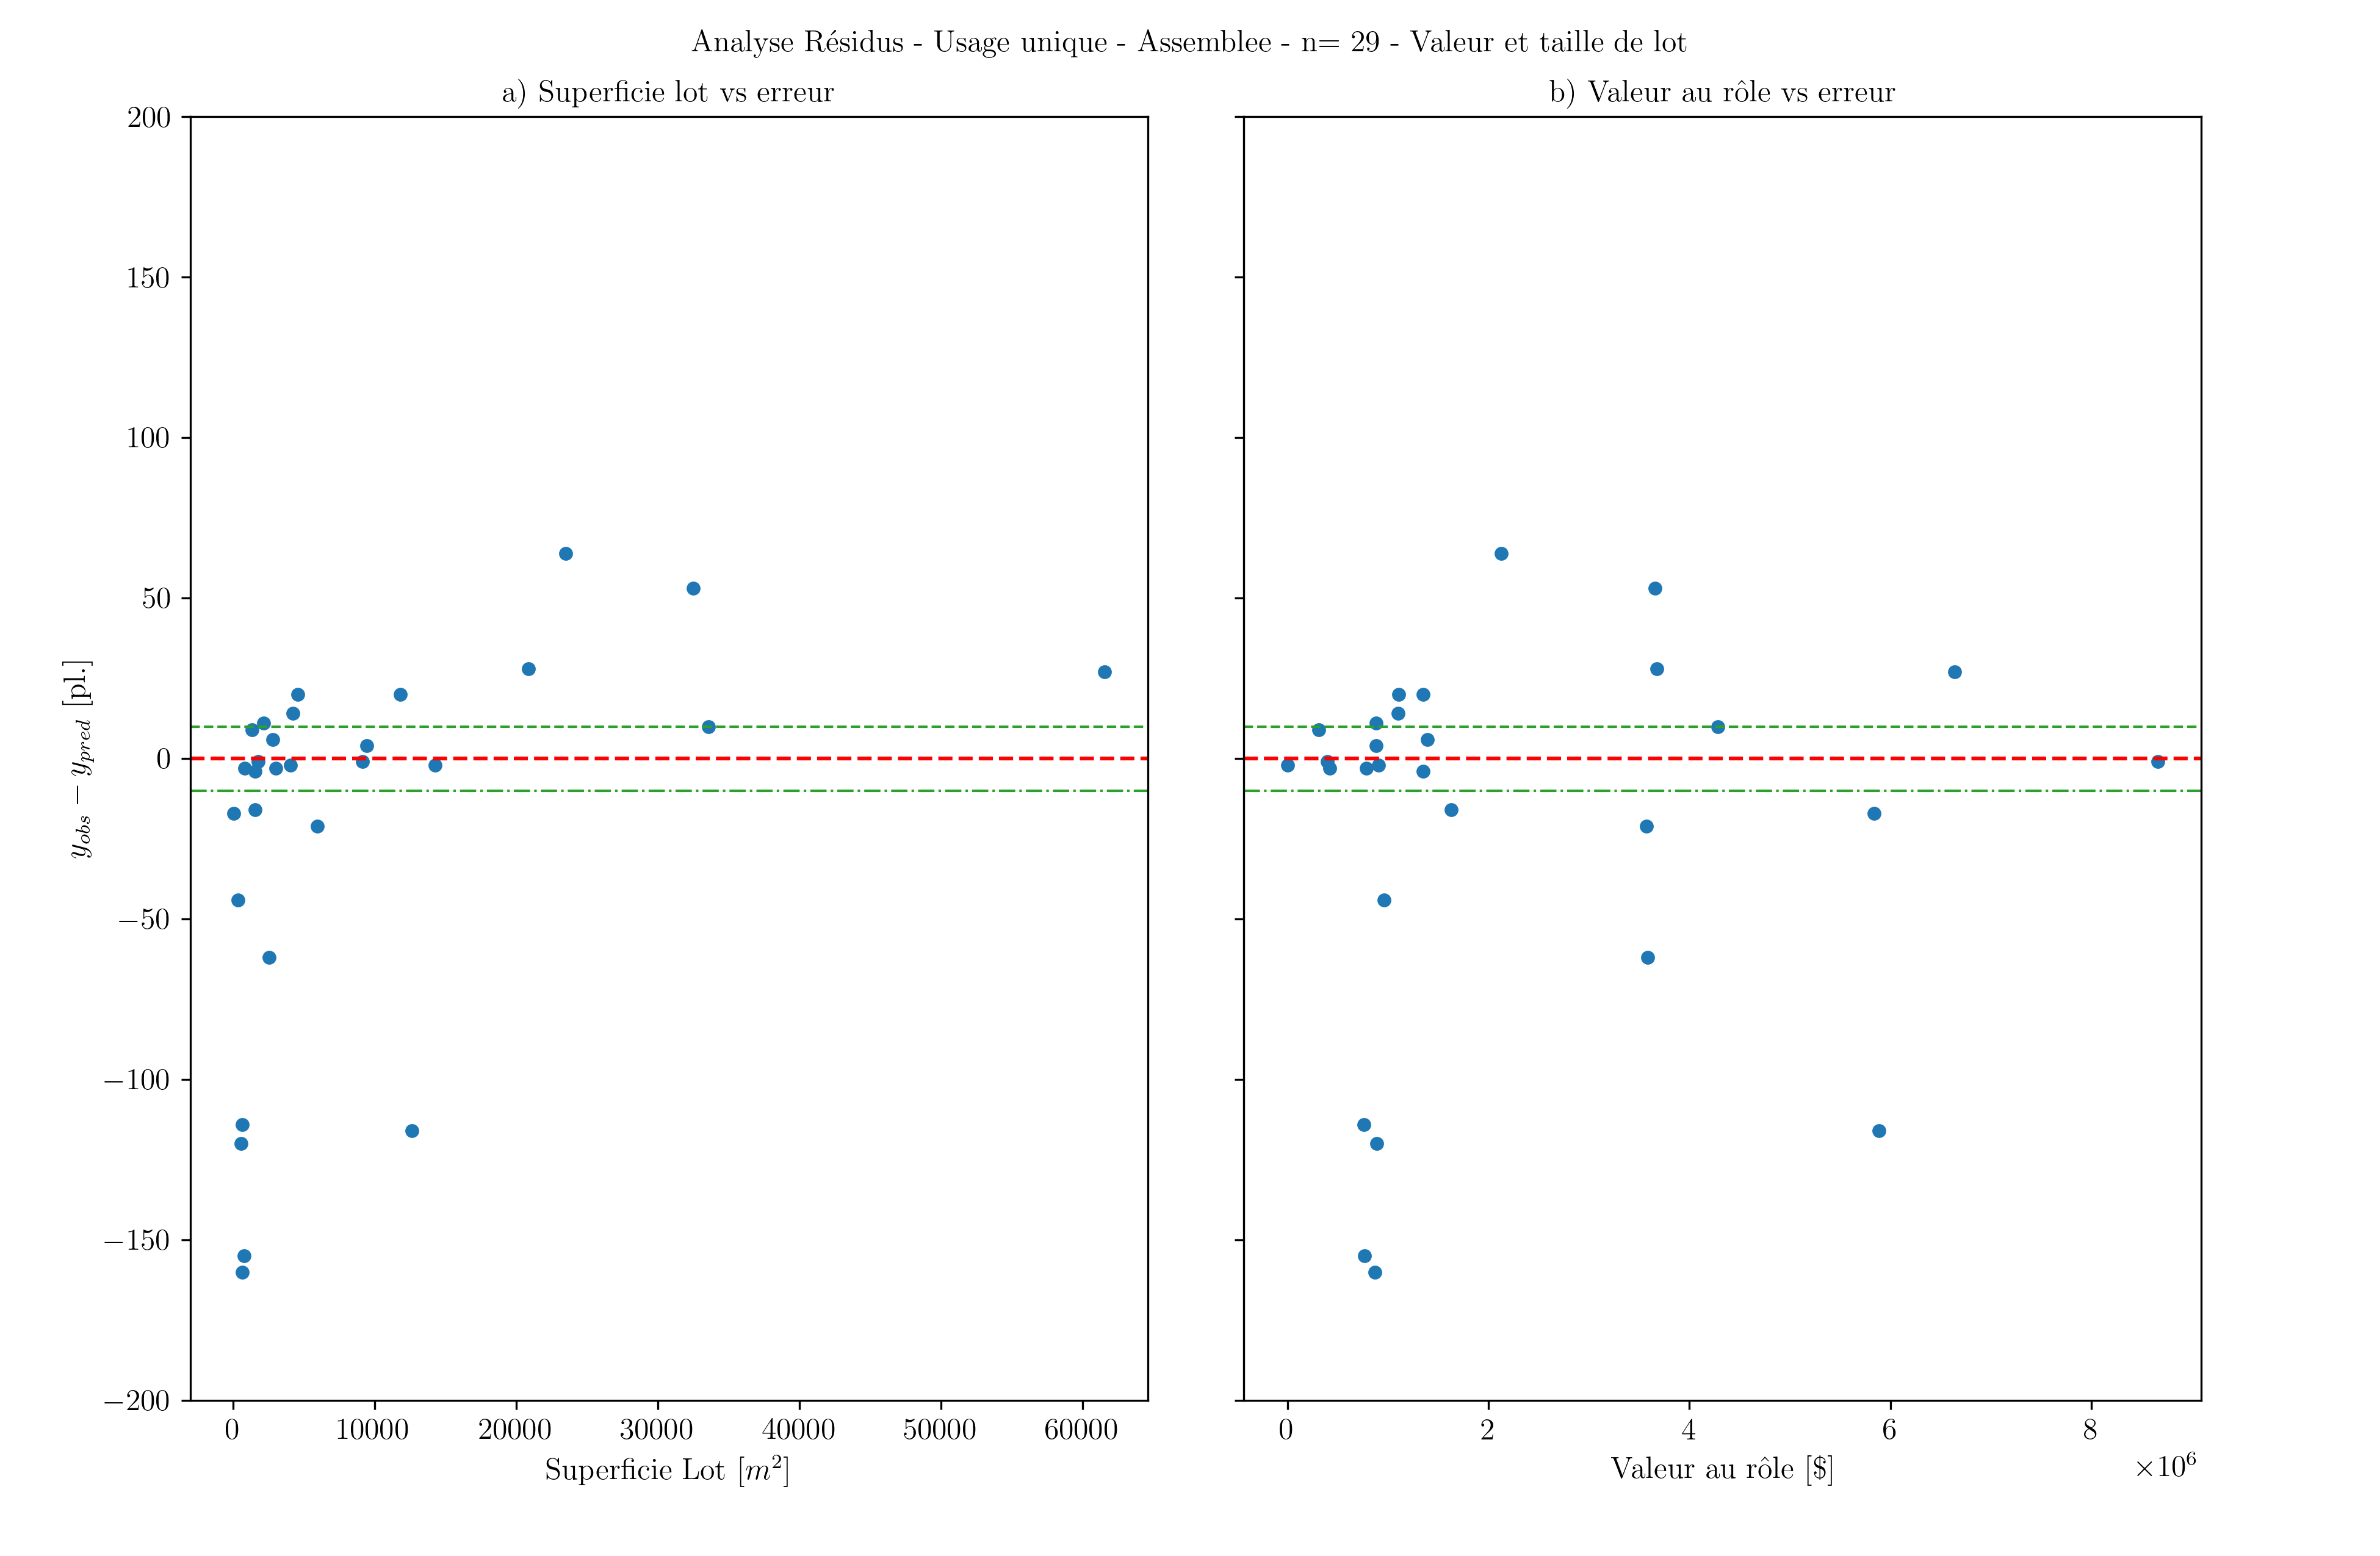
\includegraphics[width=1\linewidth]{images/ana_res_42_se_10_pe_20_d.png}
        \caption{Analyse des résidus en fonction de la superficie du lot et de la valeur pour les lots d'assemblée}
        \label{fig:ana-res-sup-val-ass}
    \end{figure}
    \begin{figure}[H]
        \centering
        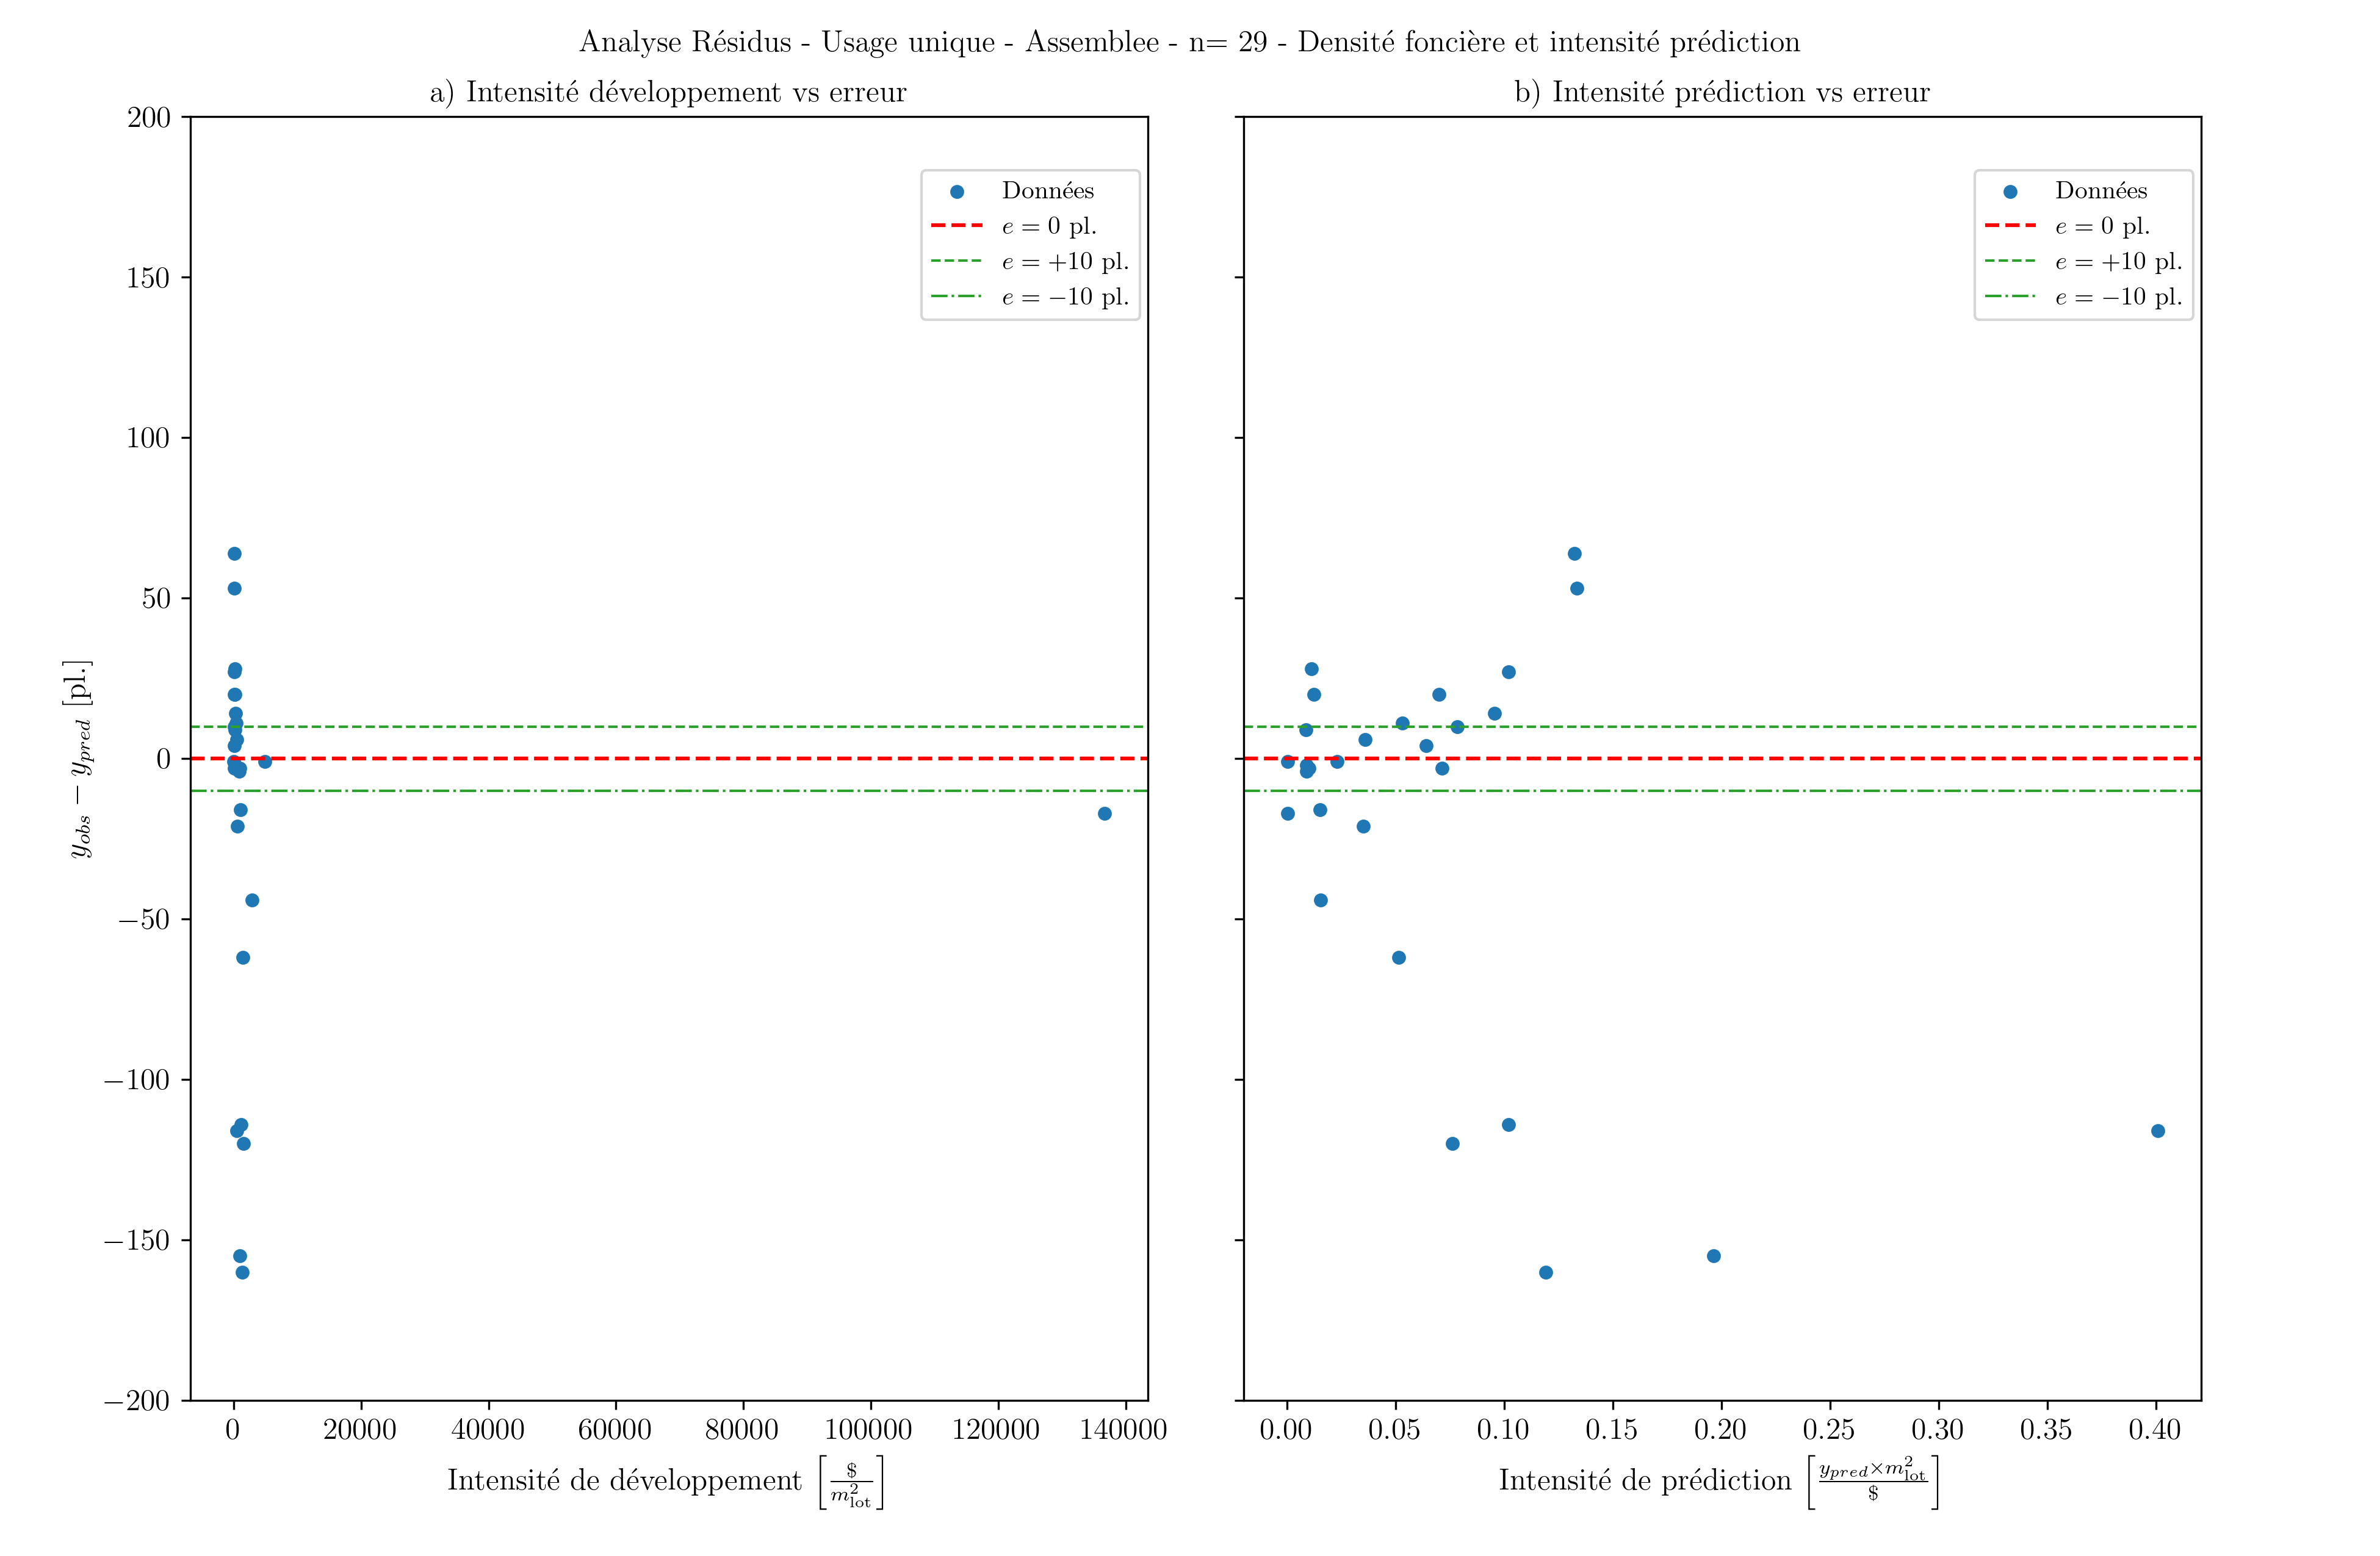
\includegraphics[width=1\linewidth]{images/ana_res_42_se_10_pe_20_e.png}
        \caption{Analyse des résidus en fonction de l'intensité de développement et l'intensité de prédiction pour les lots d'assemblée}
        \label{fig:ana-res-intens-ass}
    \end{figure}
\end{landscape}
\subsection{Usage mixte}
L'usage mixte est une autre catégorie de propriétés où le modèle a de la difficulté. Cependant, cet effet est en partie dû au fait que les propriétés à usage mixte sont plus concentrées dans les quartiers centraux, où l'offre de stationnement sur un lot est potentiellement nulle. L'apparence de ligne droite du graphique de la figure \ref{fig:ana-res-unit-pred-mix}a, visible aussi avec la rangée de valeur observée à zéro place à la figure \ref{fig:int-dist-pred-mix}a. Cette tendance fait en sorte que la moyenne du stationnement prédit est très supérieure à la valeur observée.
\begin{figure}[H]
    \centering
    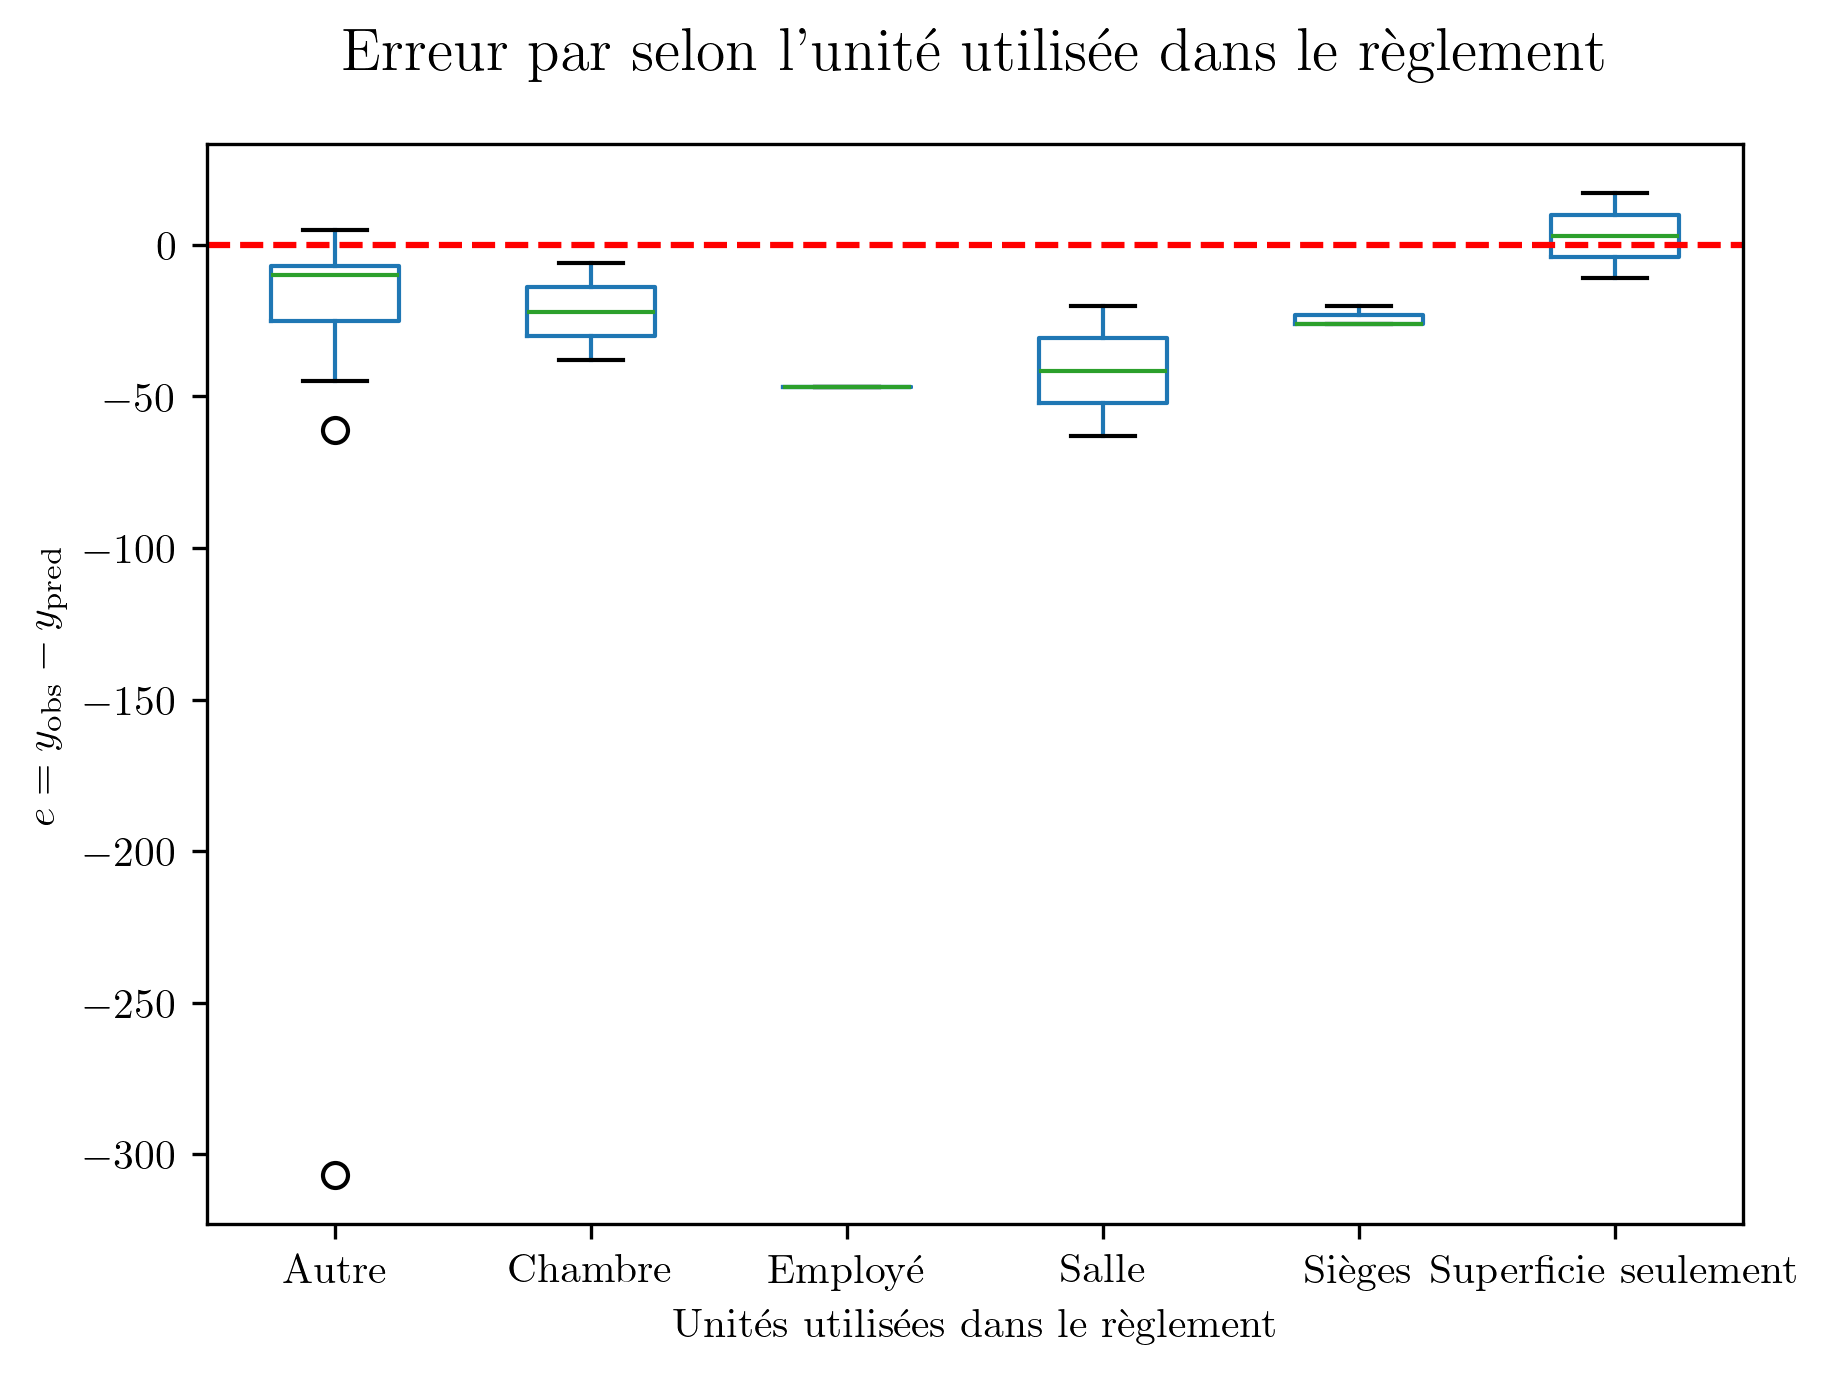
\includegraphics[width=1\linewidth]{images/boxplot_error_by_category_34.png}
    \caption{Erreur de la catégorie usage mixte selon l'unité de formulation du règlement}
    \label{fig:boxplot-erreur-usmixte-unite}
\end{figure}
\begin{landscape}
    %\begin{figure}
    %    \centering
    %    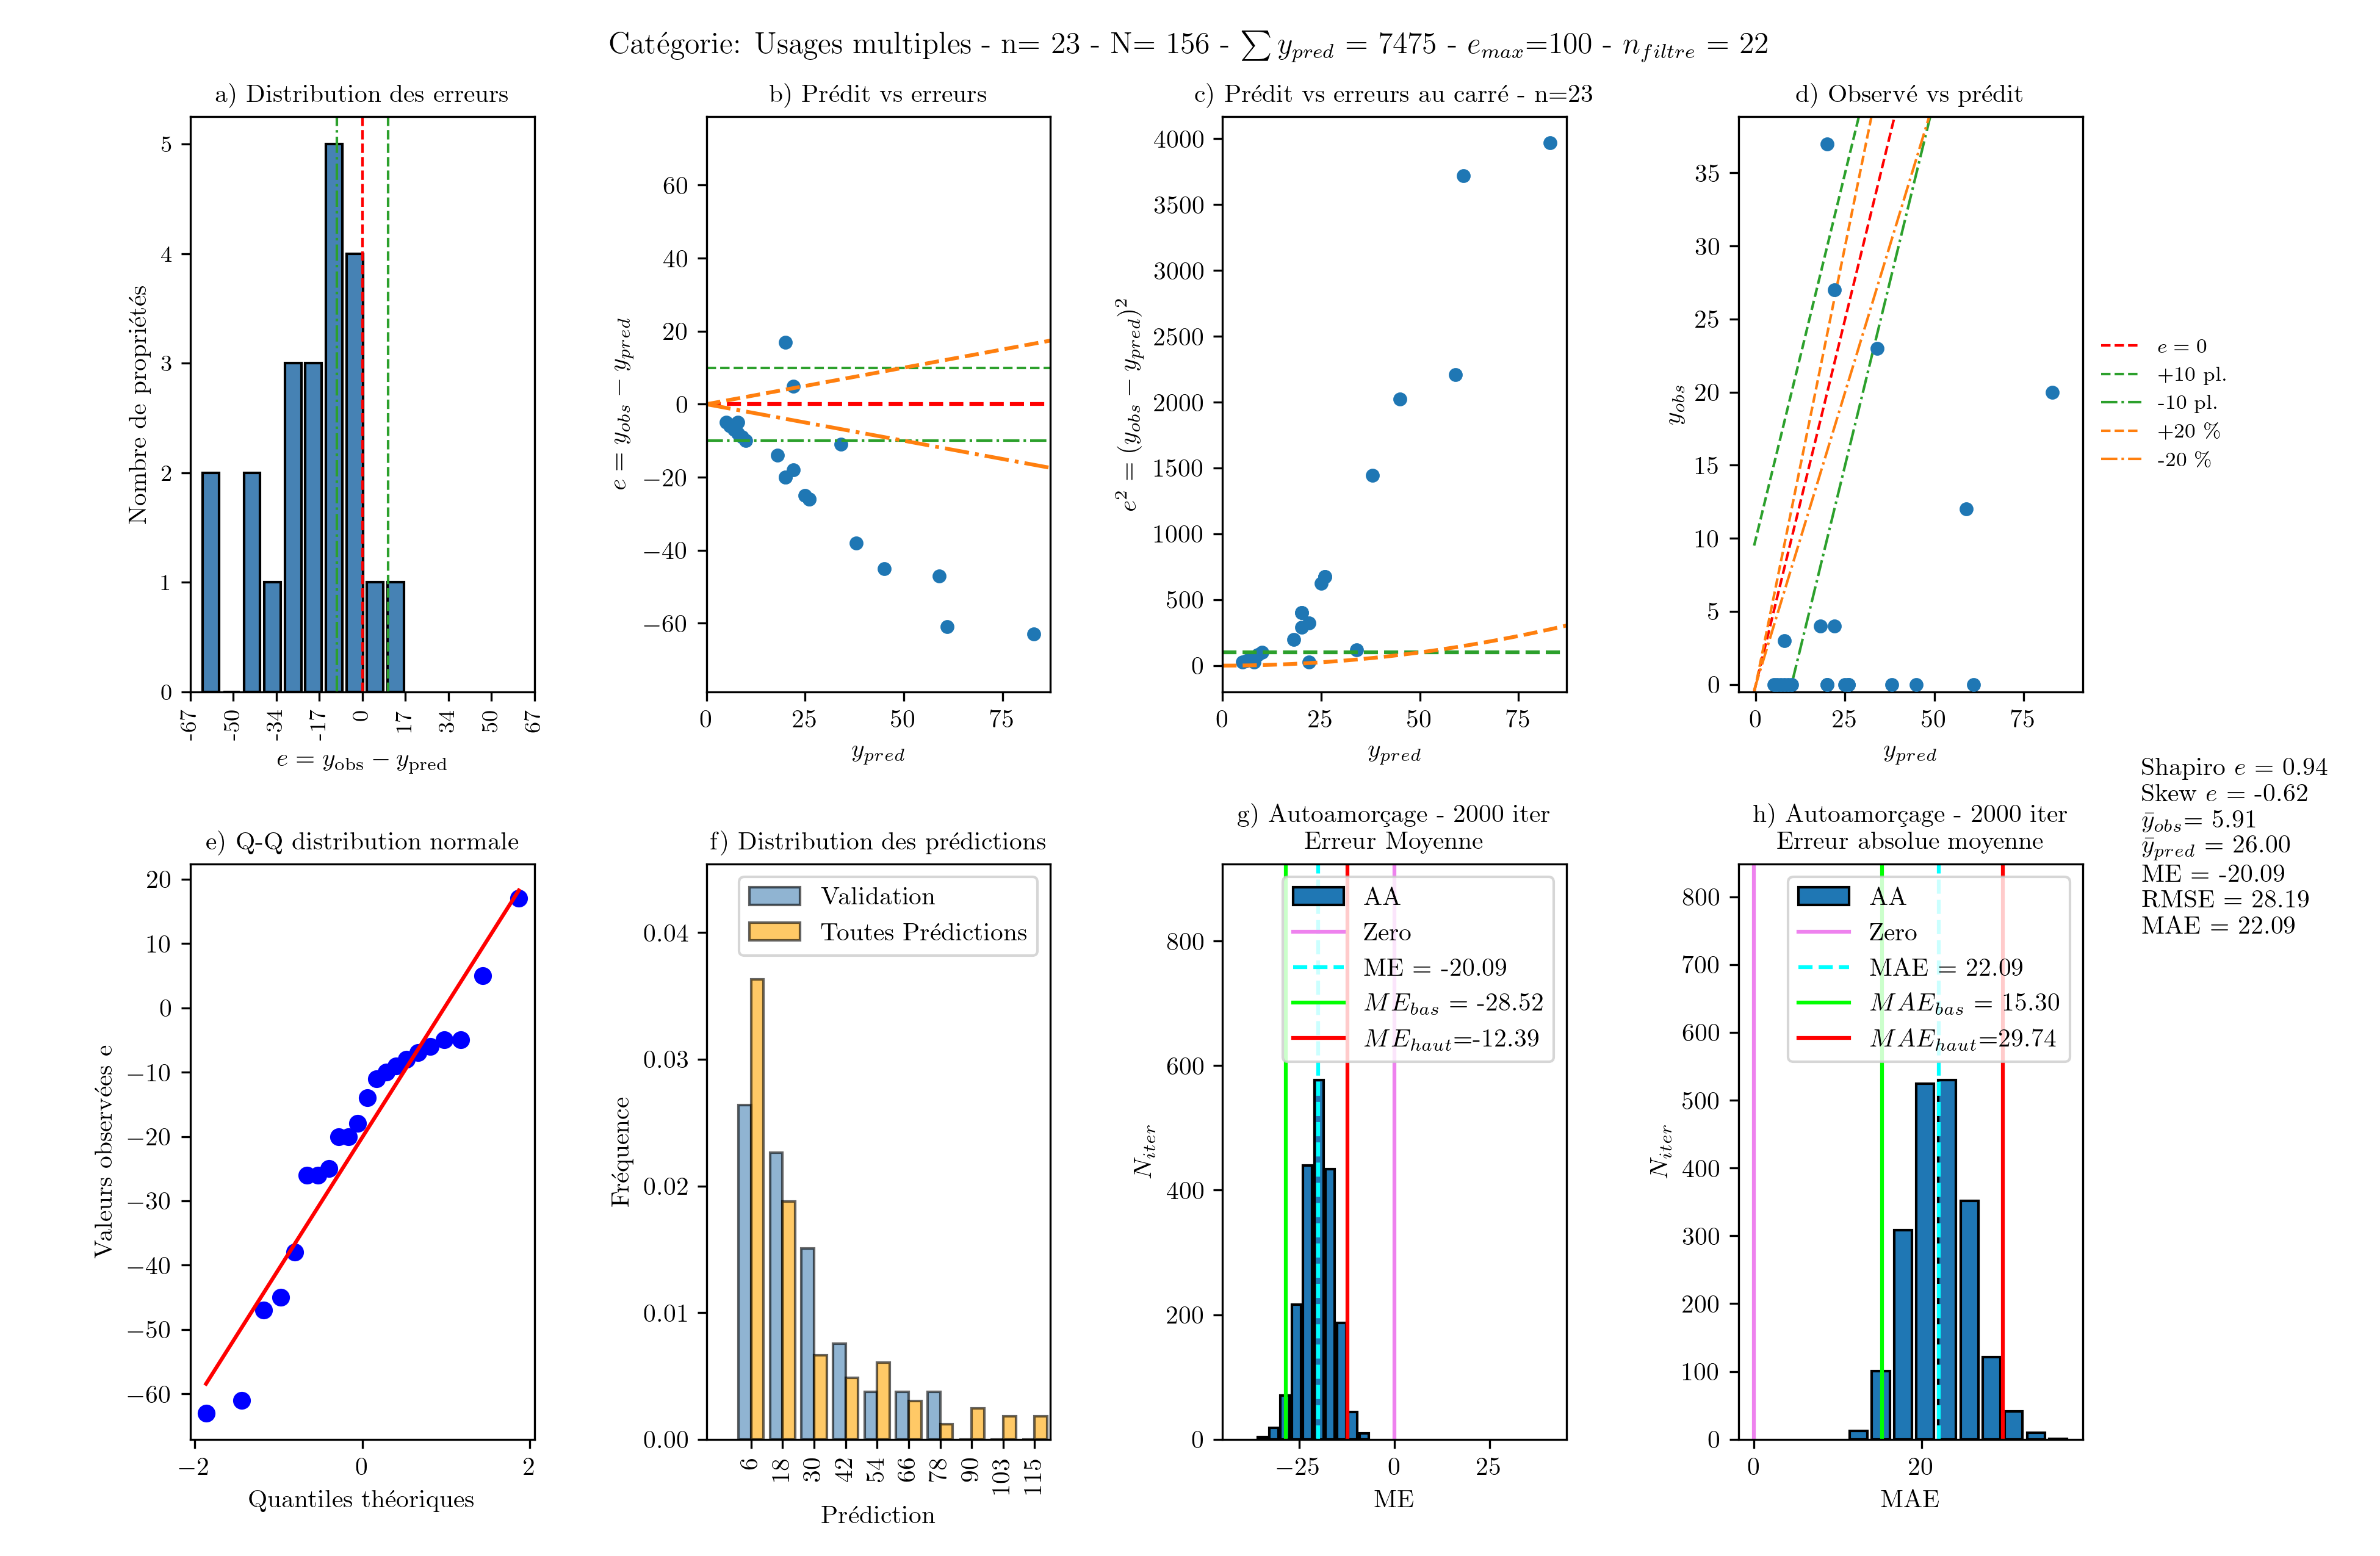
\includegraphics[scale=0.65]{images/int_erreur_34_e_100_se_10_pe_20.png}
    %    \caption{Distribution et intervalles d'erreurs pour les lots d'usage mixte avec une erreur maximale fixée à 100 places}
    %    \label{fig:intervals-dis-val-mix-e100}
    %\end{figure}
    \begin{figure}[H]
        \centering
        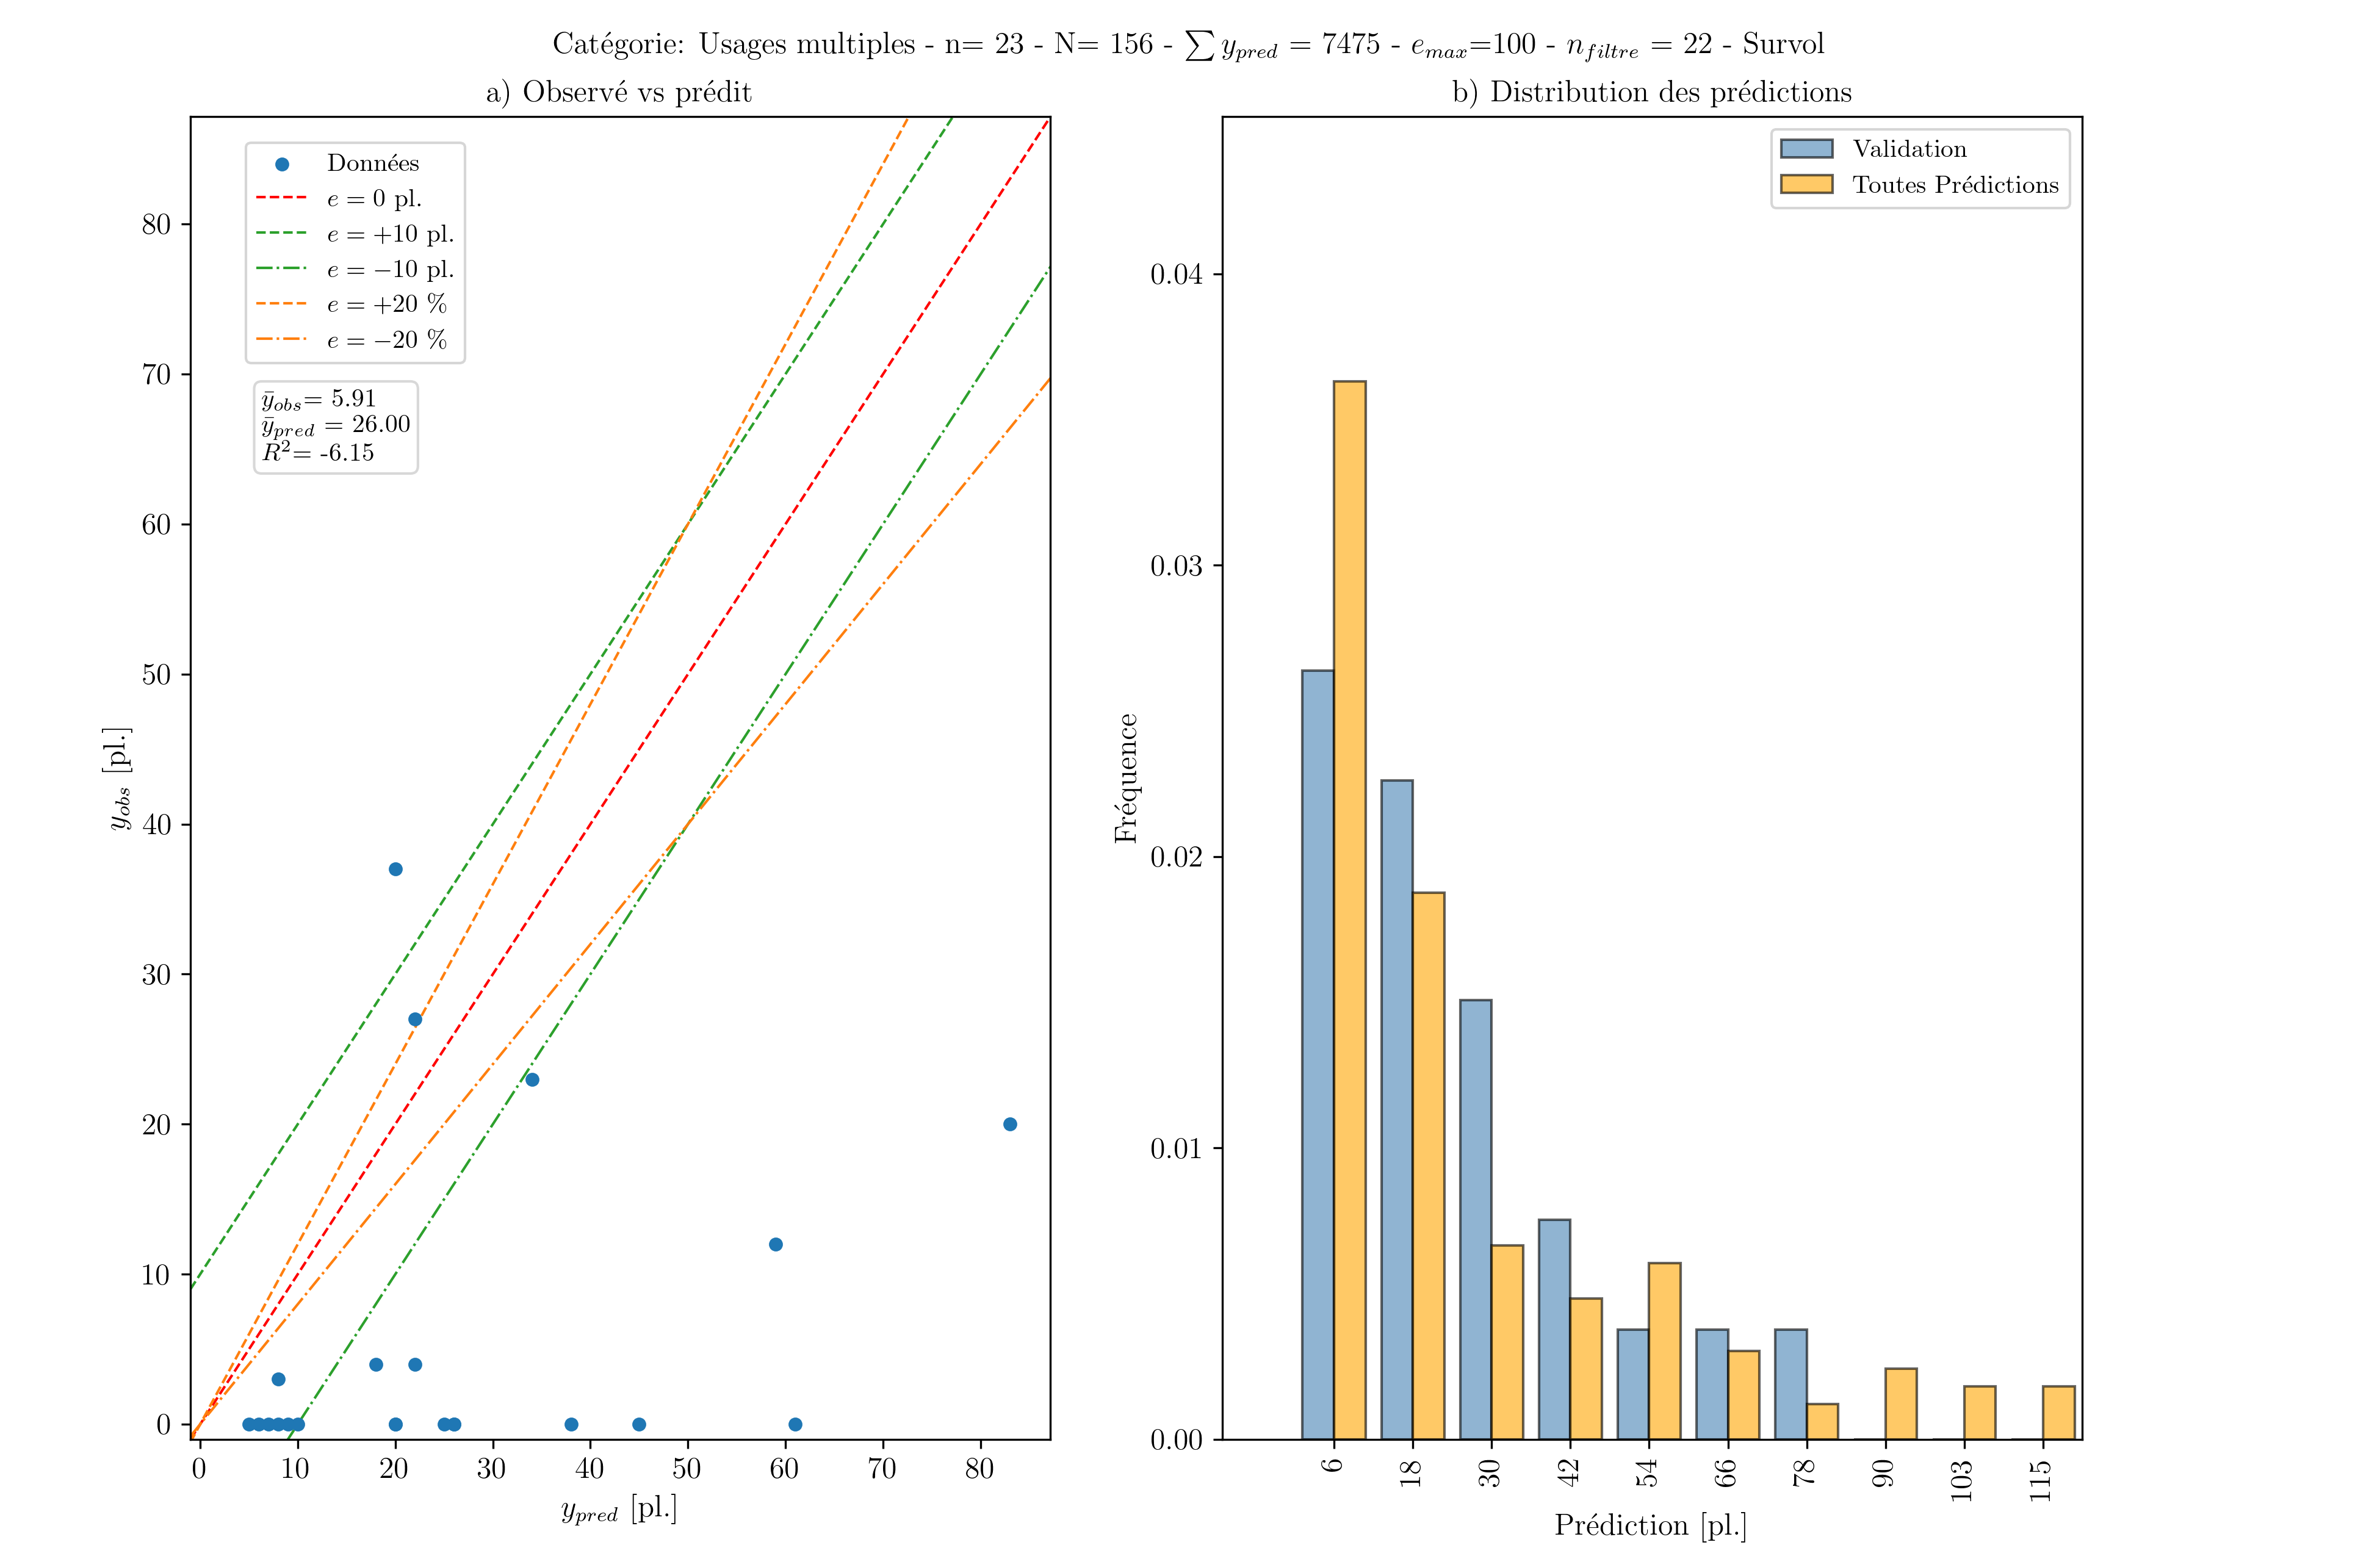
\includegraphics[width=1\linewidth]{images/int_erreur_34_e_100_se_10_pe_20_a.png}
        \caption{Distribution des prédictions pour les lots d'usage mixte}
        \label{fig:int-dist-pred-mix}
    \end{figure}
    \begin{figure}[H]
        \centering
        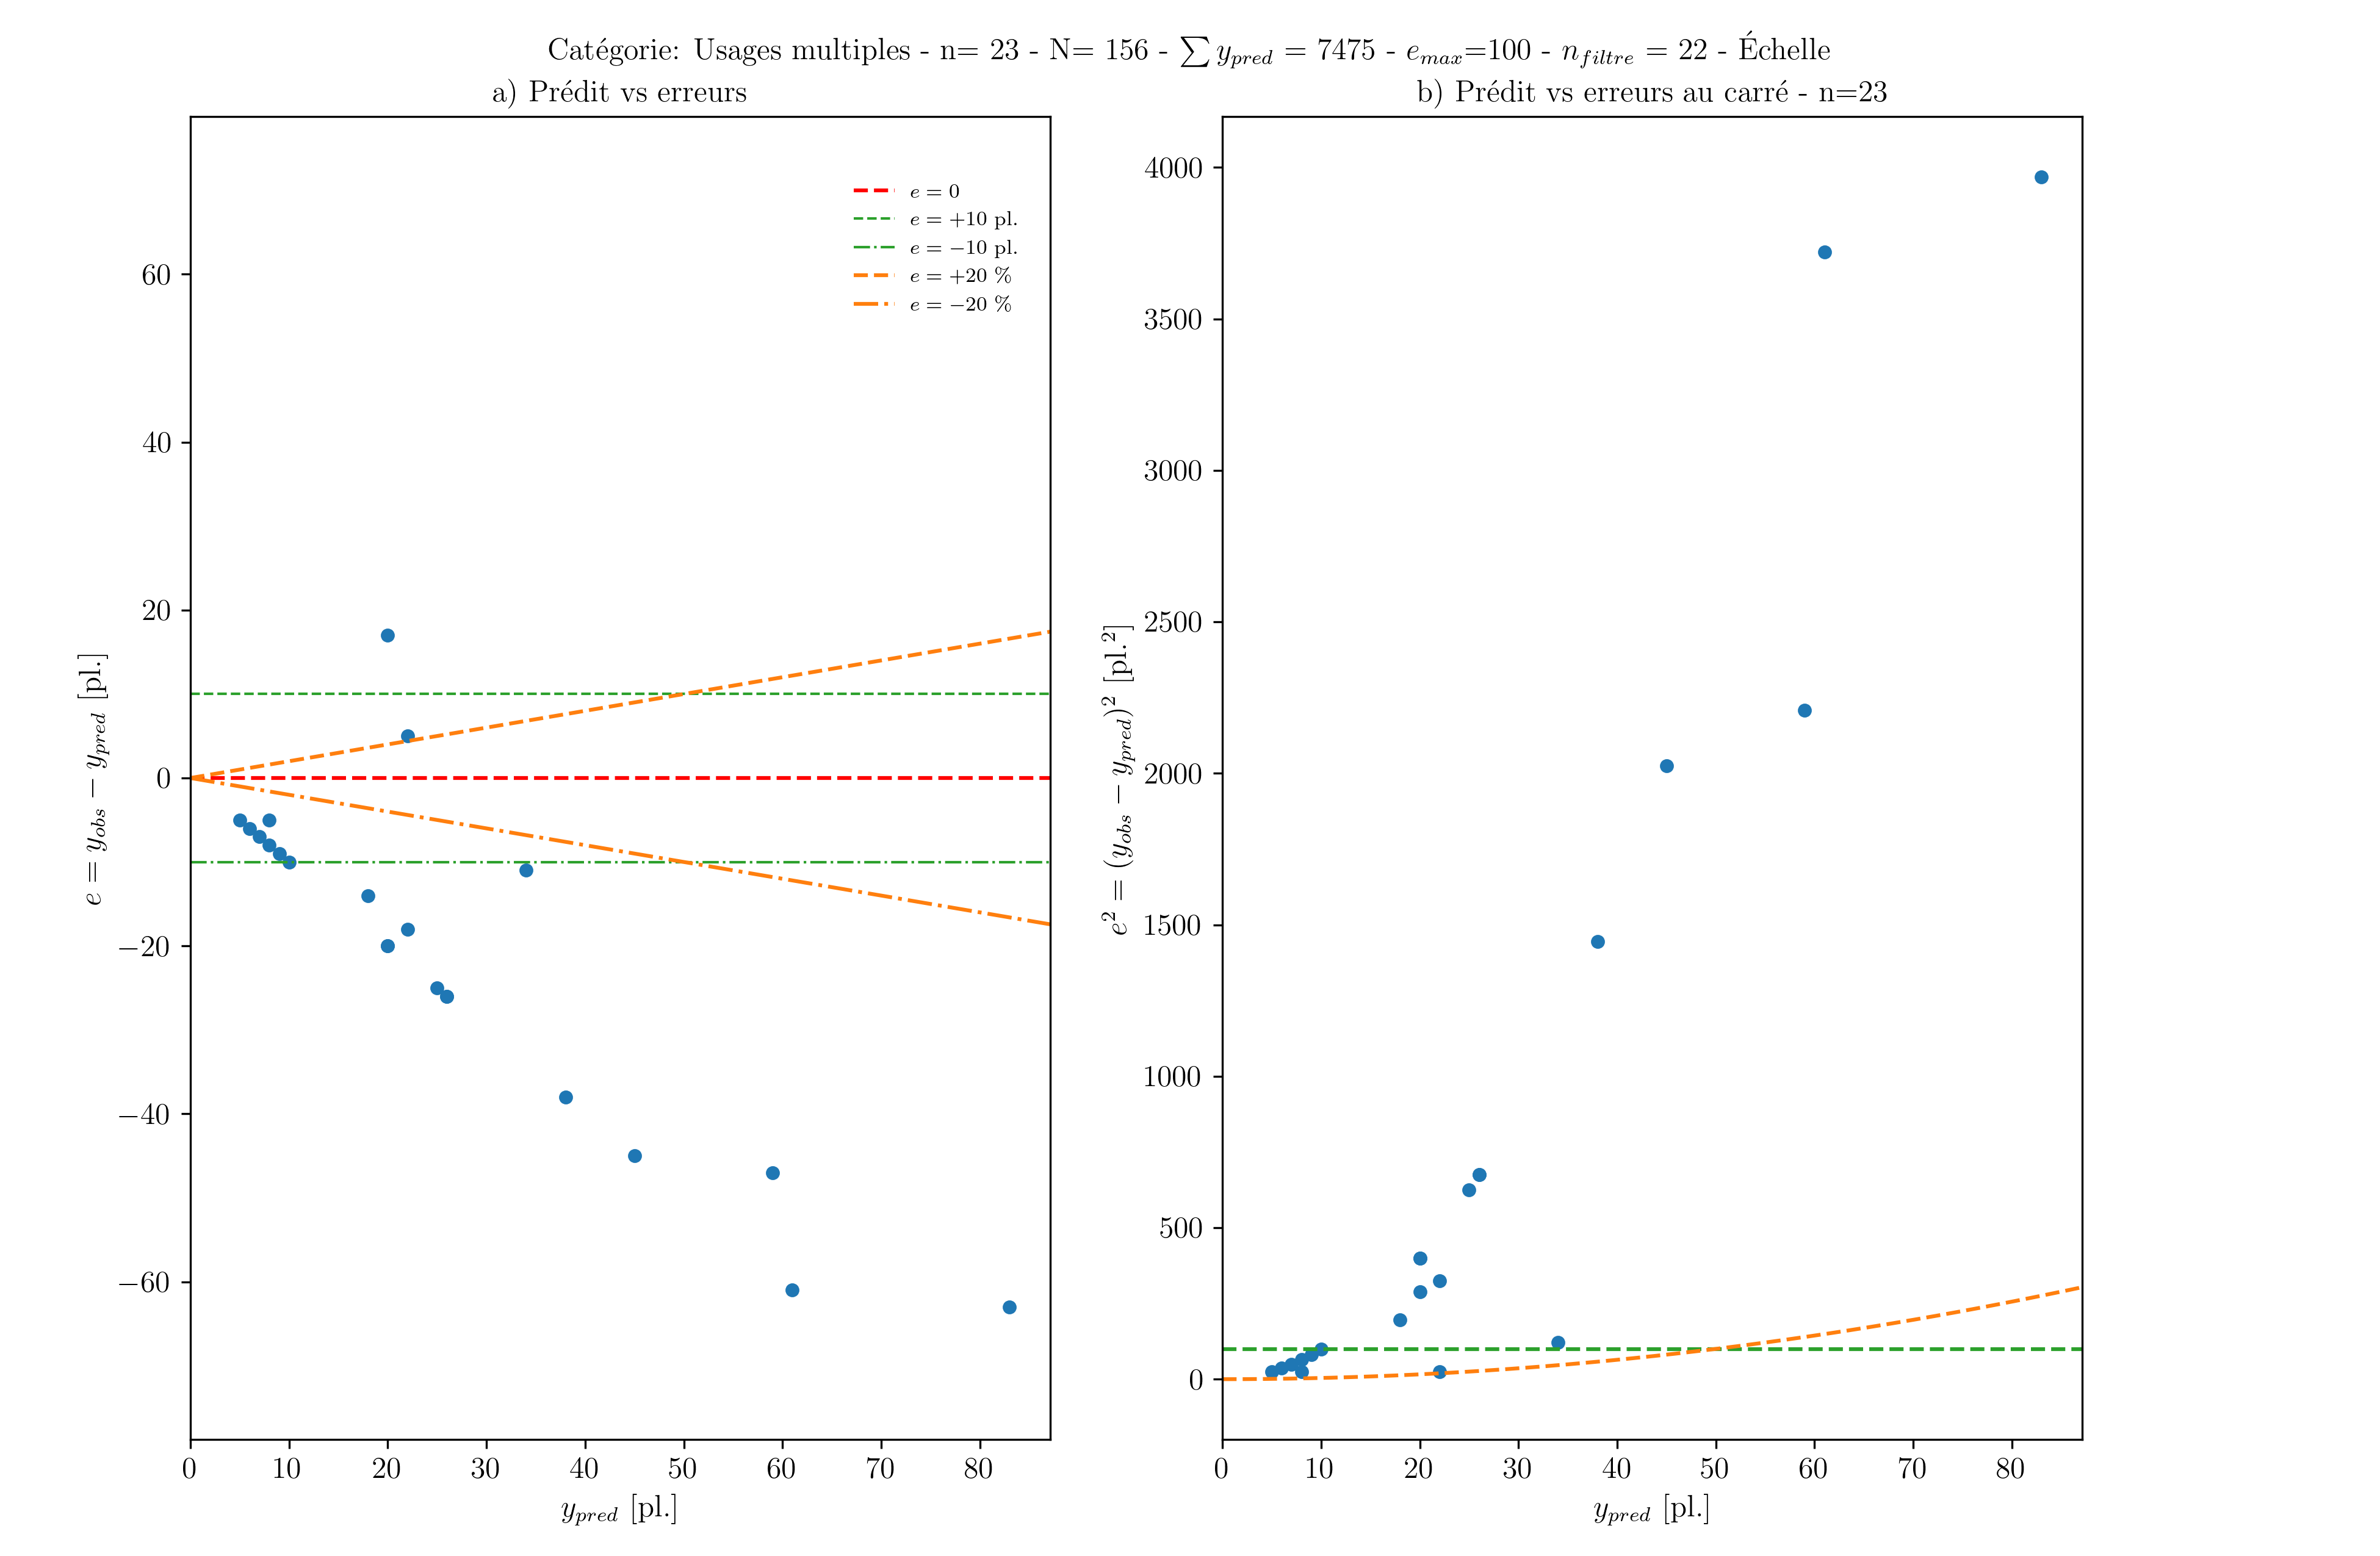
\includegraphics[width=1\linewidth]{images/int_erreur_34_e_100_se_10_pe_20_b.png}
        \caption{Erreur en fonction des prédictions pour les lots d'usage mixte}
        \label{fig:err-err-quad-pred-mix}
    \end{figure}
    \begin{figure}[H]
        \centering
        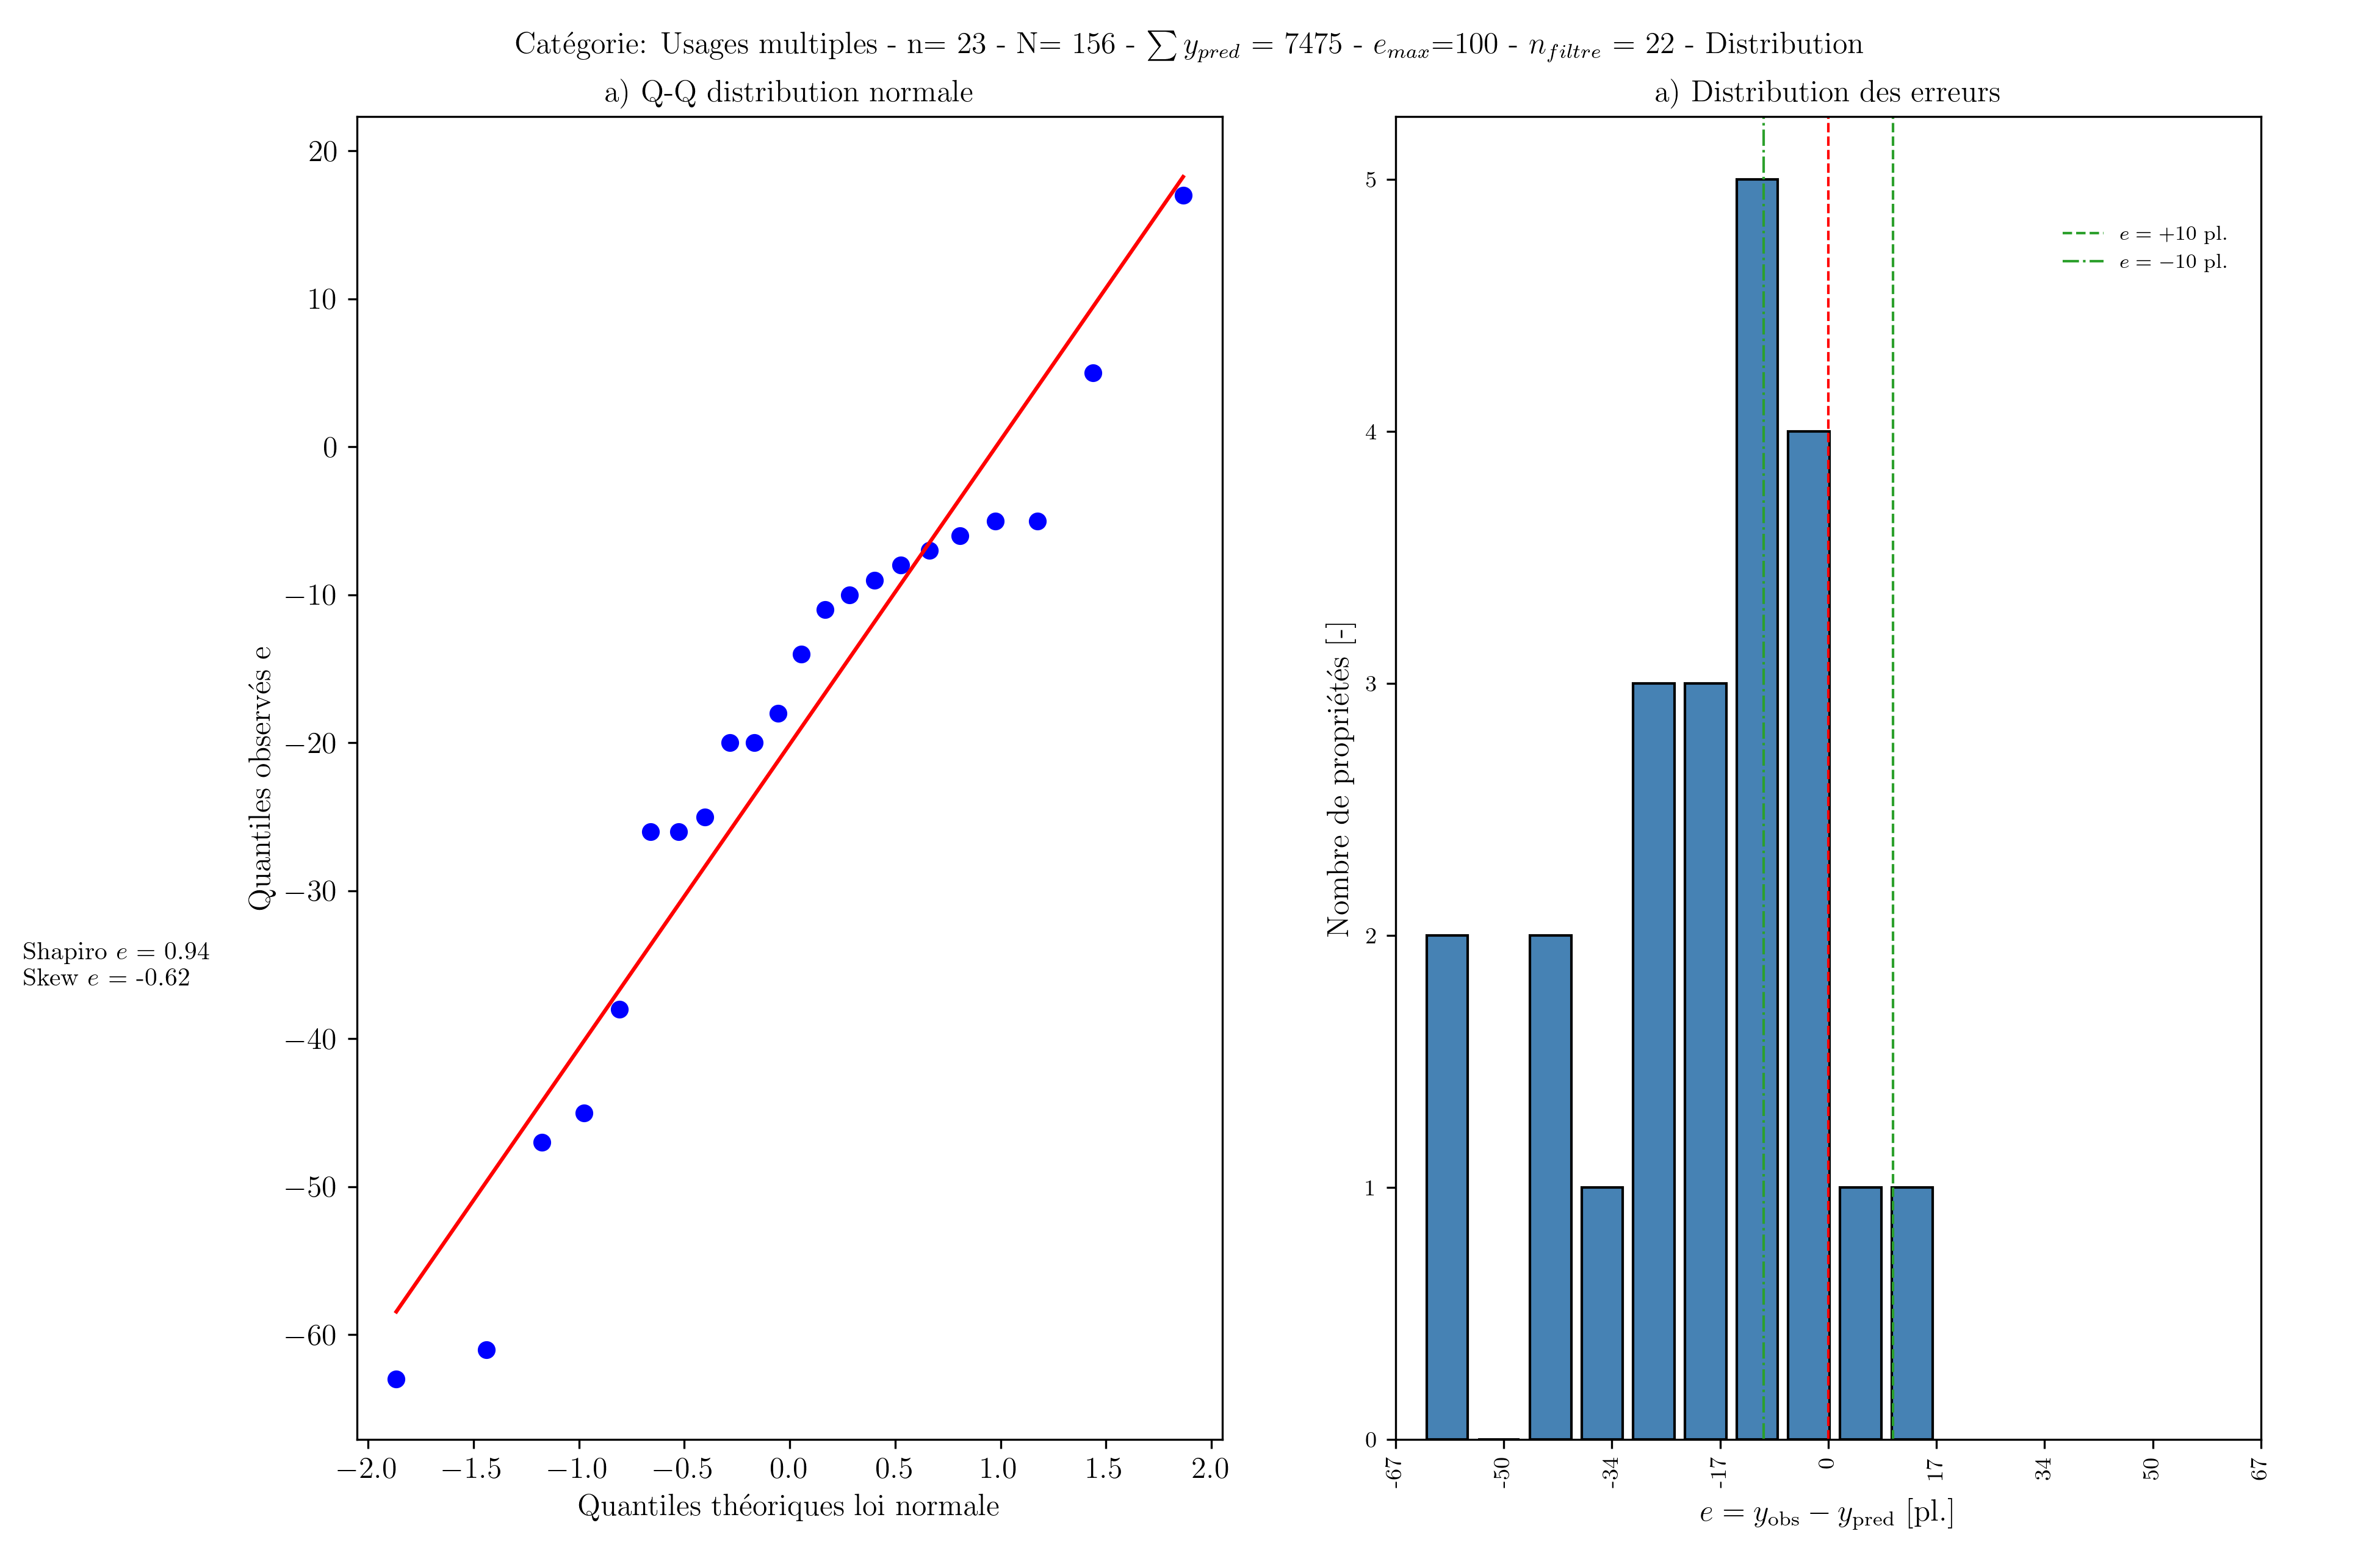
\includegraphics[width=1\linewidth]{images/int_erreur_34_e_100_se_10_pe_20_c.png}
        \caption{Distribution et normalité des erreurs pour les lots d'usage mixte}
        \label{fig:dist-erreur-norm-mix}
    \end{figure}
    \begin{figure}[H]
        \centering
        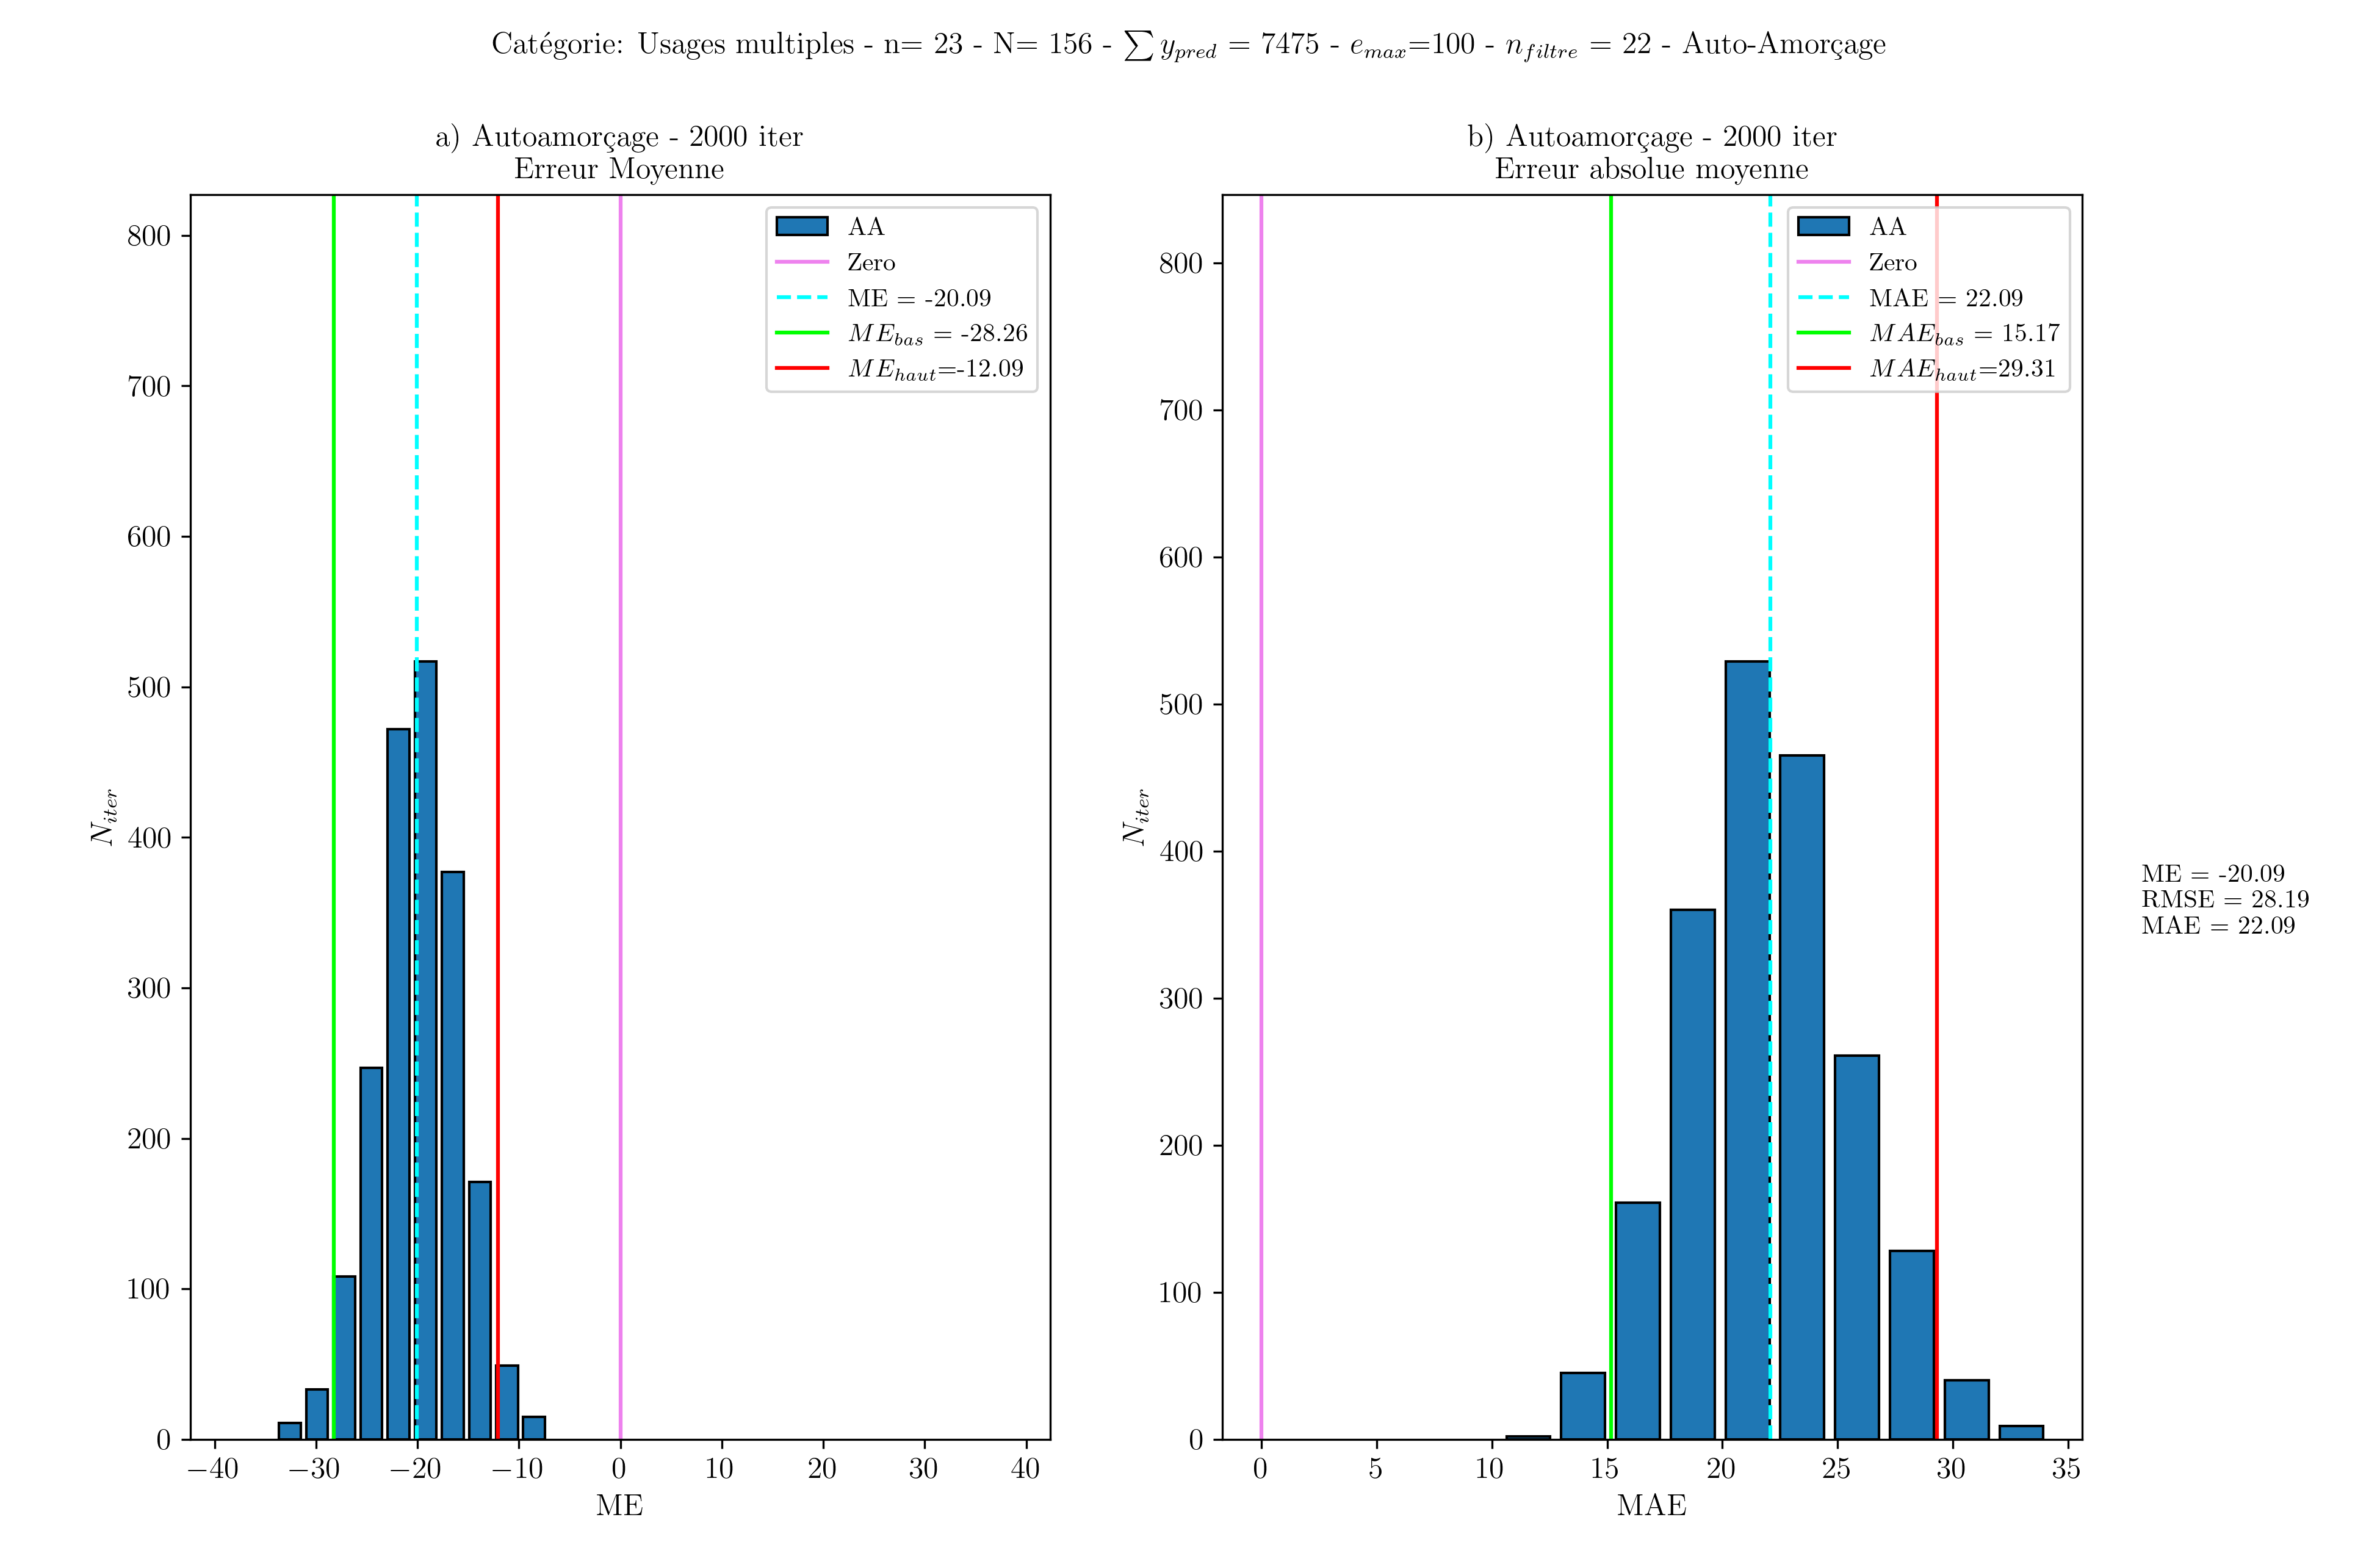
\includegraphics[width=1\linewidth]{images/int_erreur_34_e_100_se_10_pe_20_d.png}
        \caption{Distribution des métriques d'erreur après auto-amorçage pour les lots d'usage mixte}
        \label{fig:auto-amor-mix}
    \end{figure}
    %\begin{figure}[H]
    %    \centering
    %    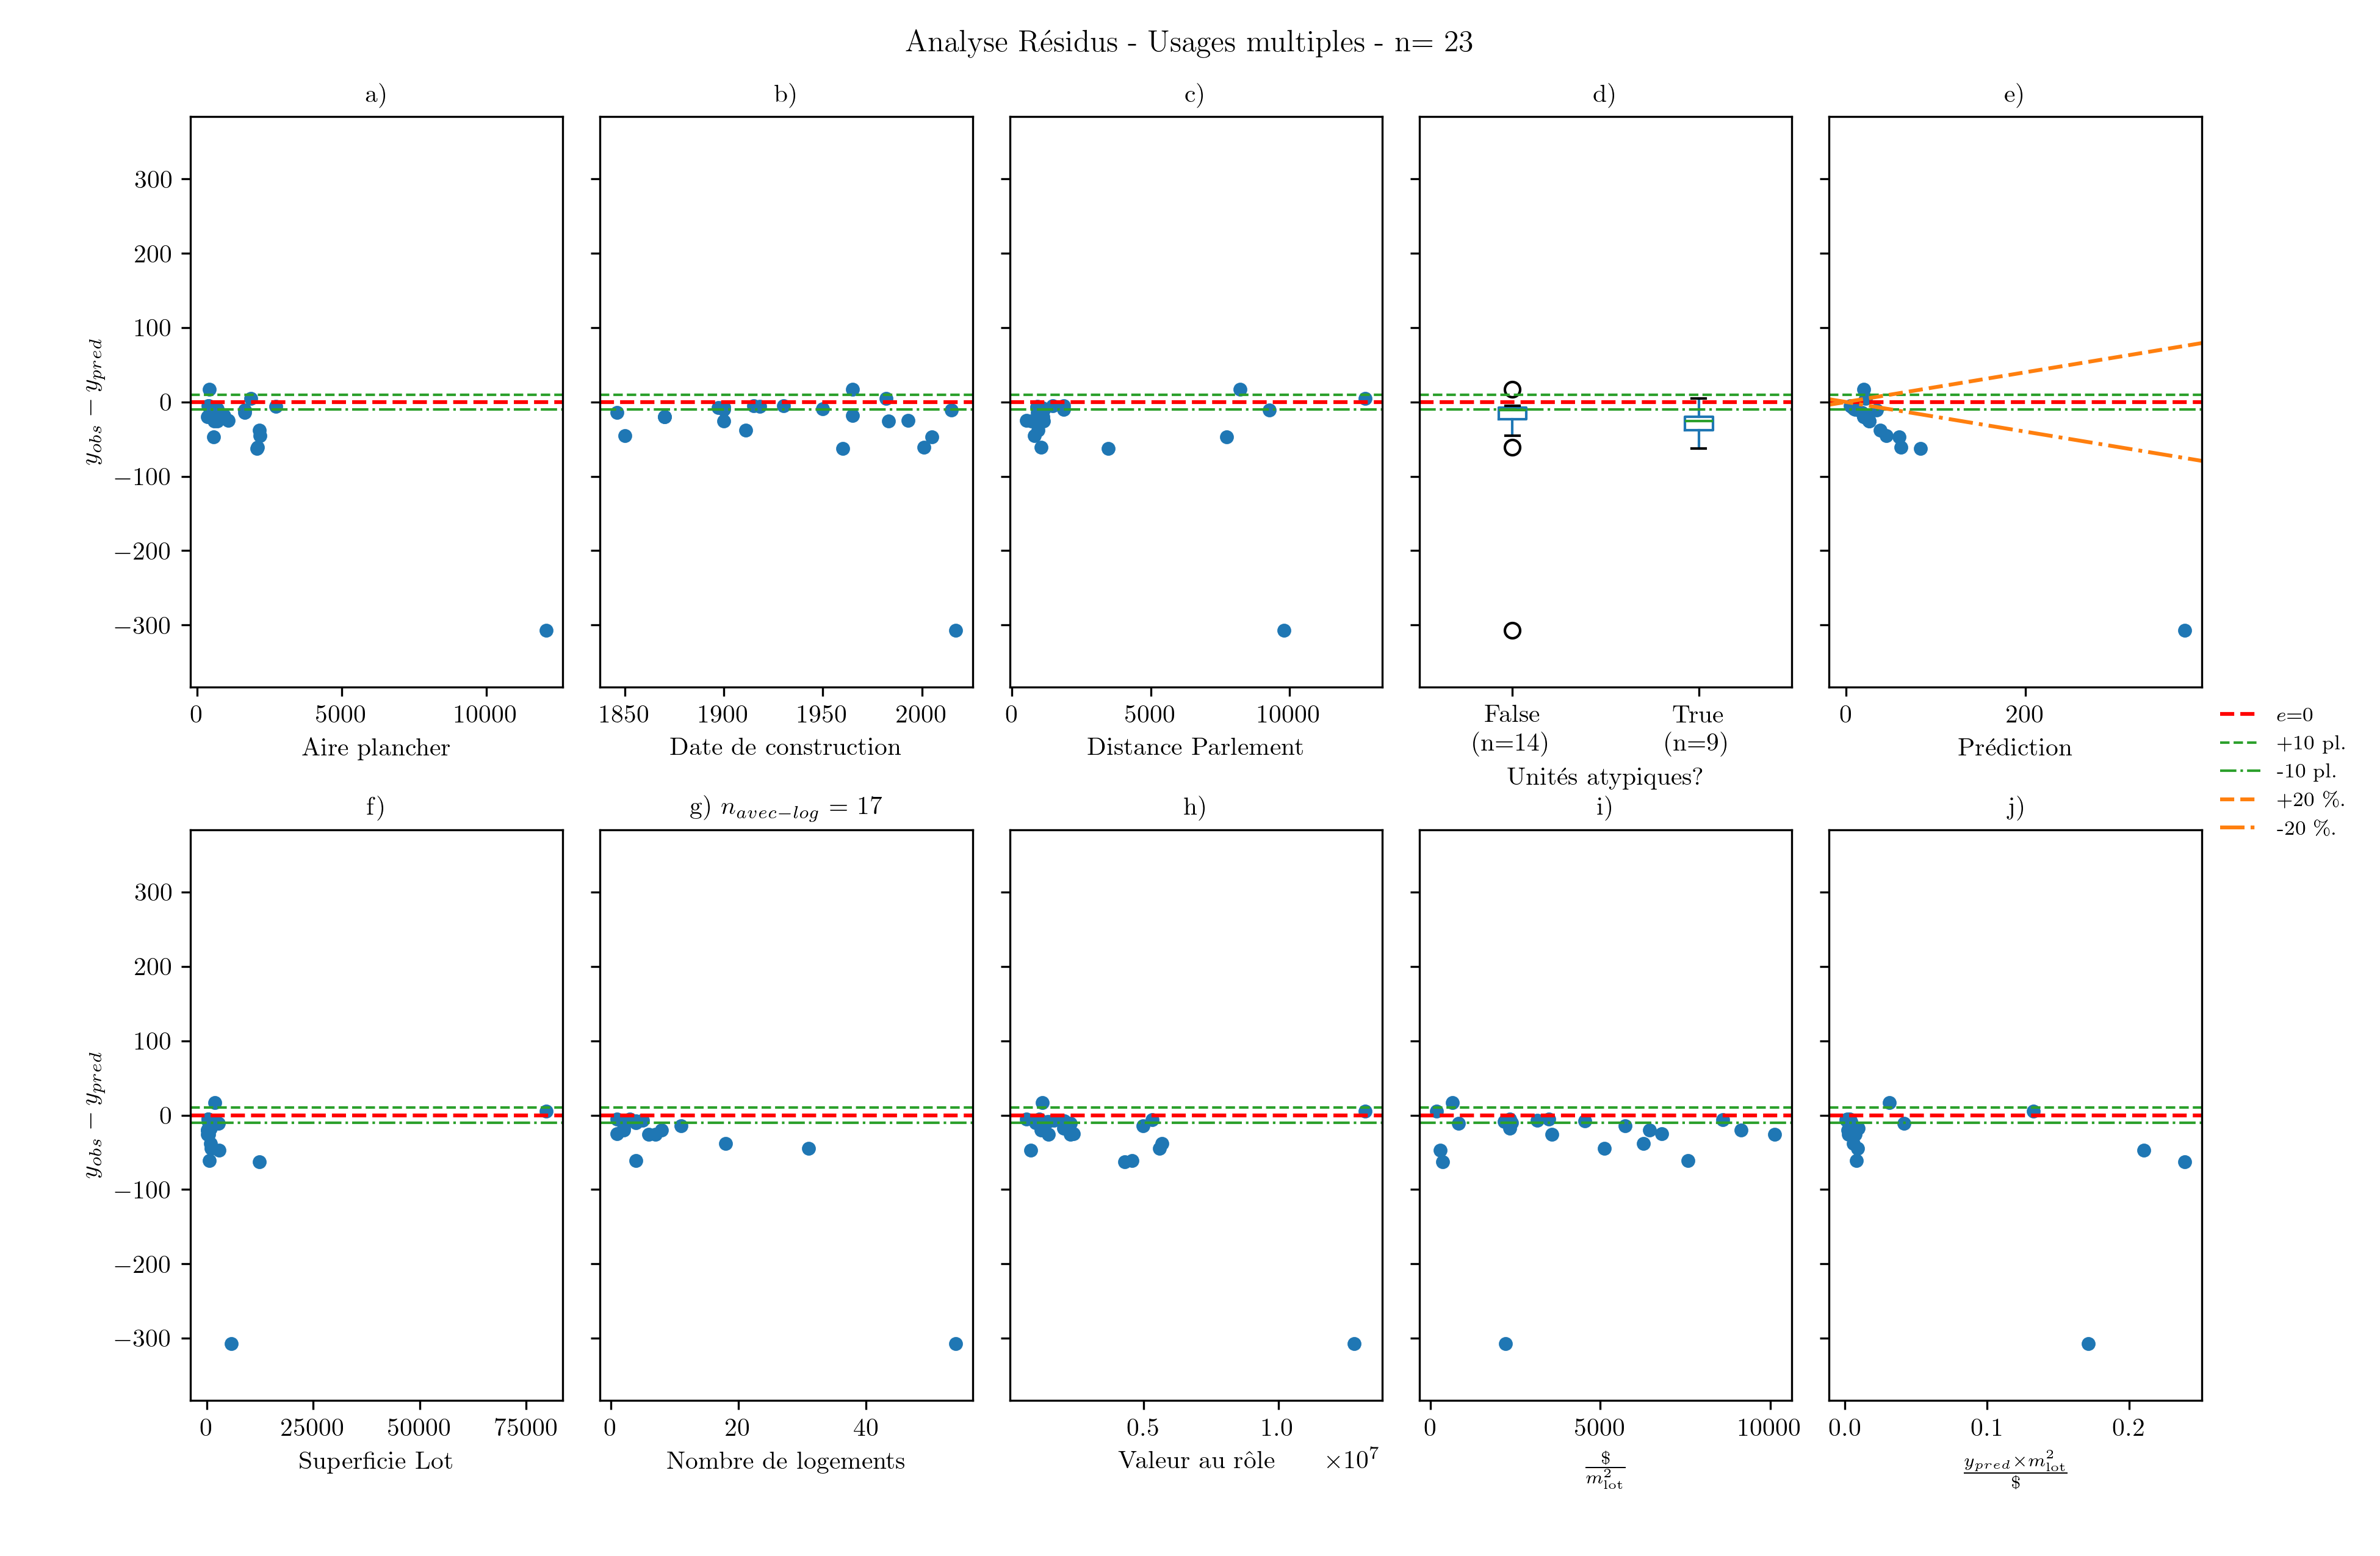
\includegraphics[scale=0.65]{images/ana_res_34_se_10_pe_20.png}
    %    \caption{Analyse des propriétés d'usage mixte sans filtre sur le nombre de places}
    %    \label{fig:ana-residu-mix}
    %\end{figure}
    \begin{figure}[H]
        \centering
        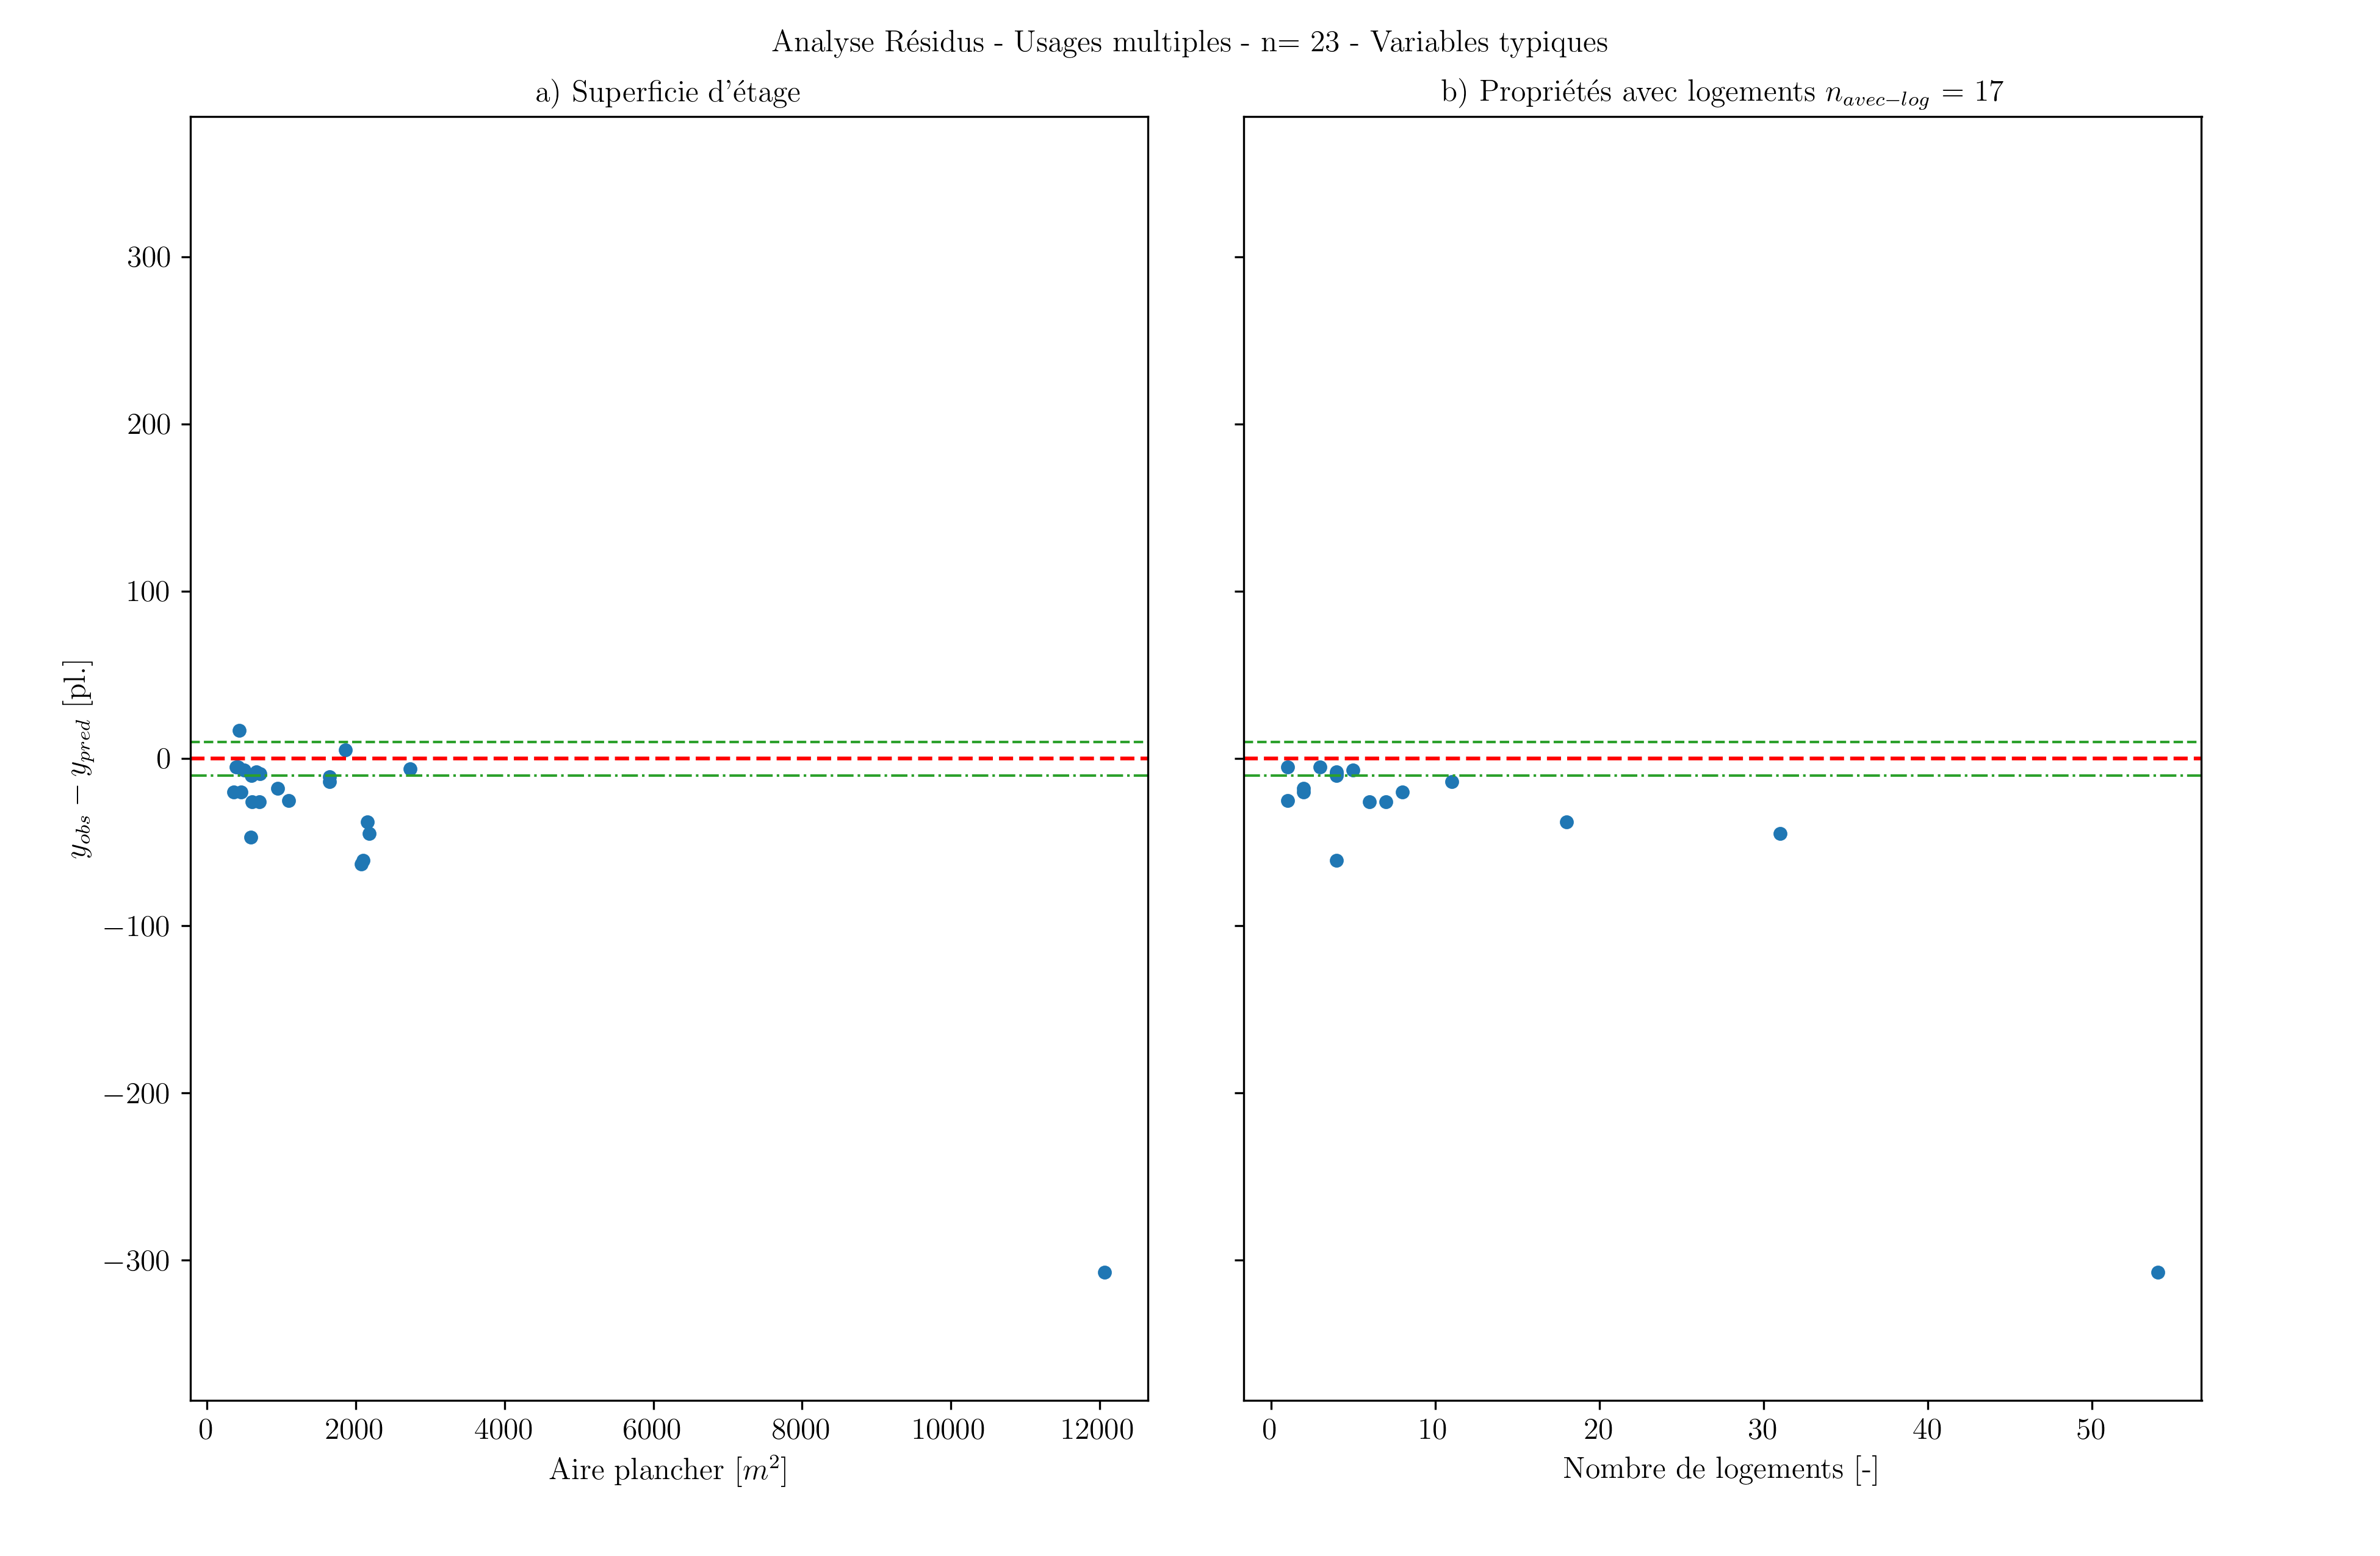
\includegraphics[width=1\linewidth]{images/ana_res_34_se_10_pe_20_a.png}
        \caption{Analyse des résidus en fonction des propriétés de construction pour les lots d'usage mixte}
        \label{fig:ana-res-prop-phys-mix}
    \end{figure}
    \begin{figure}[H]
        \centering
        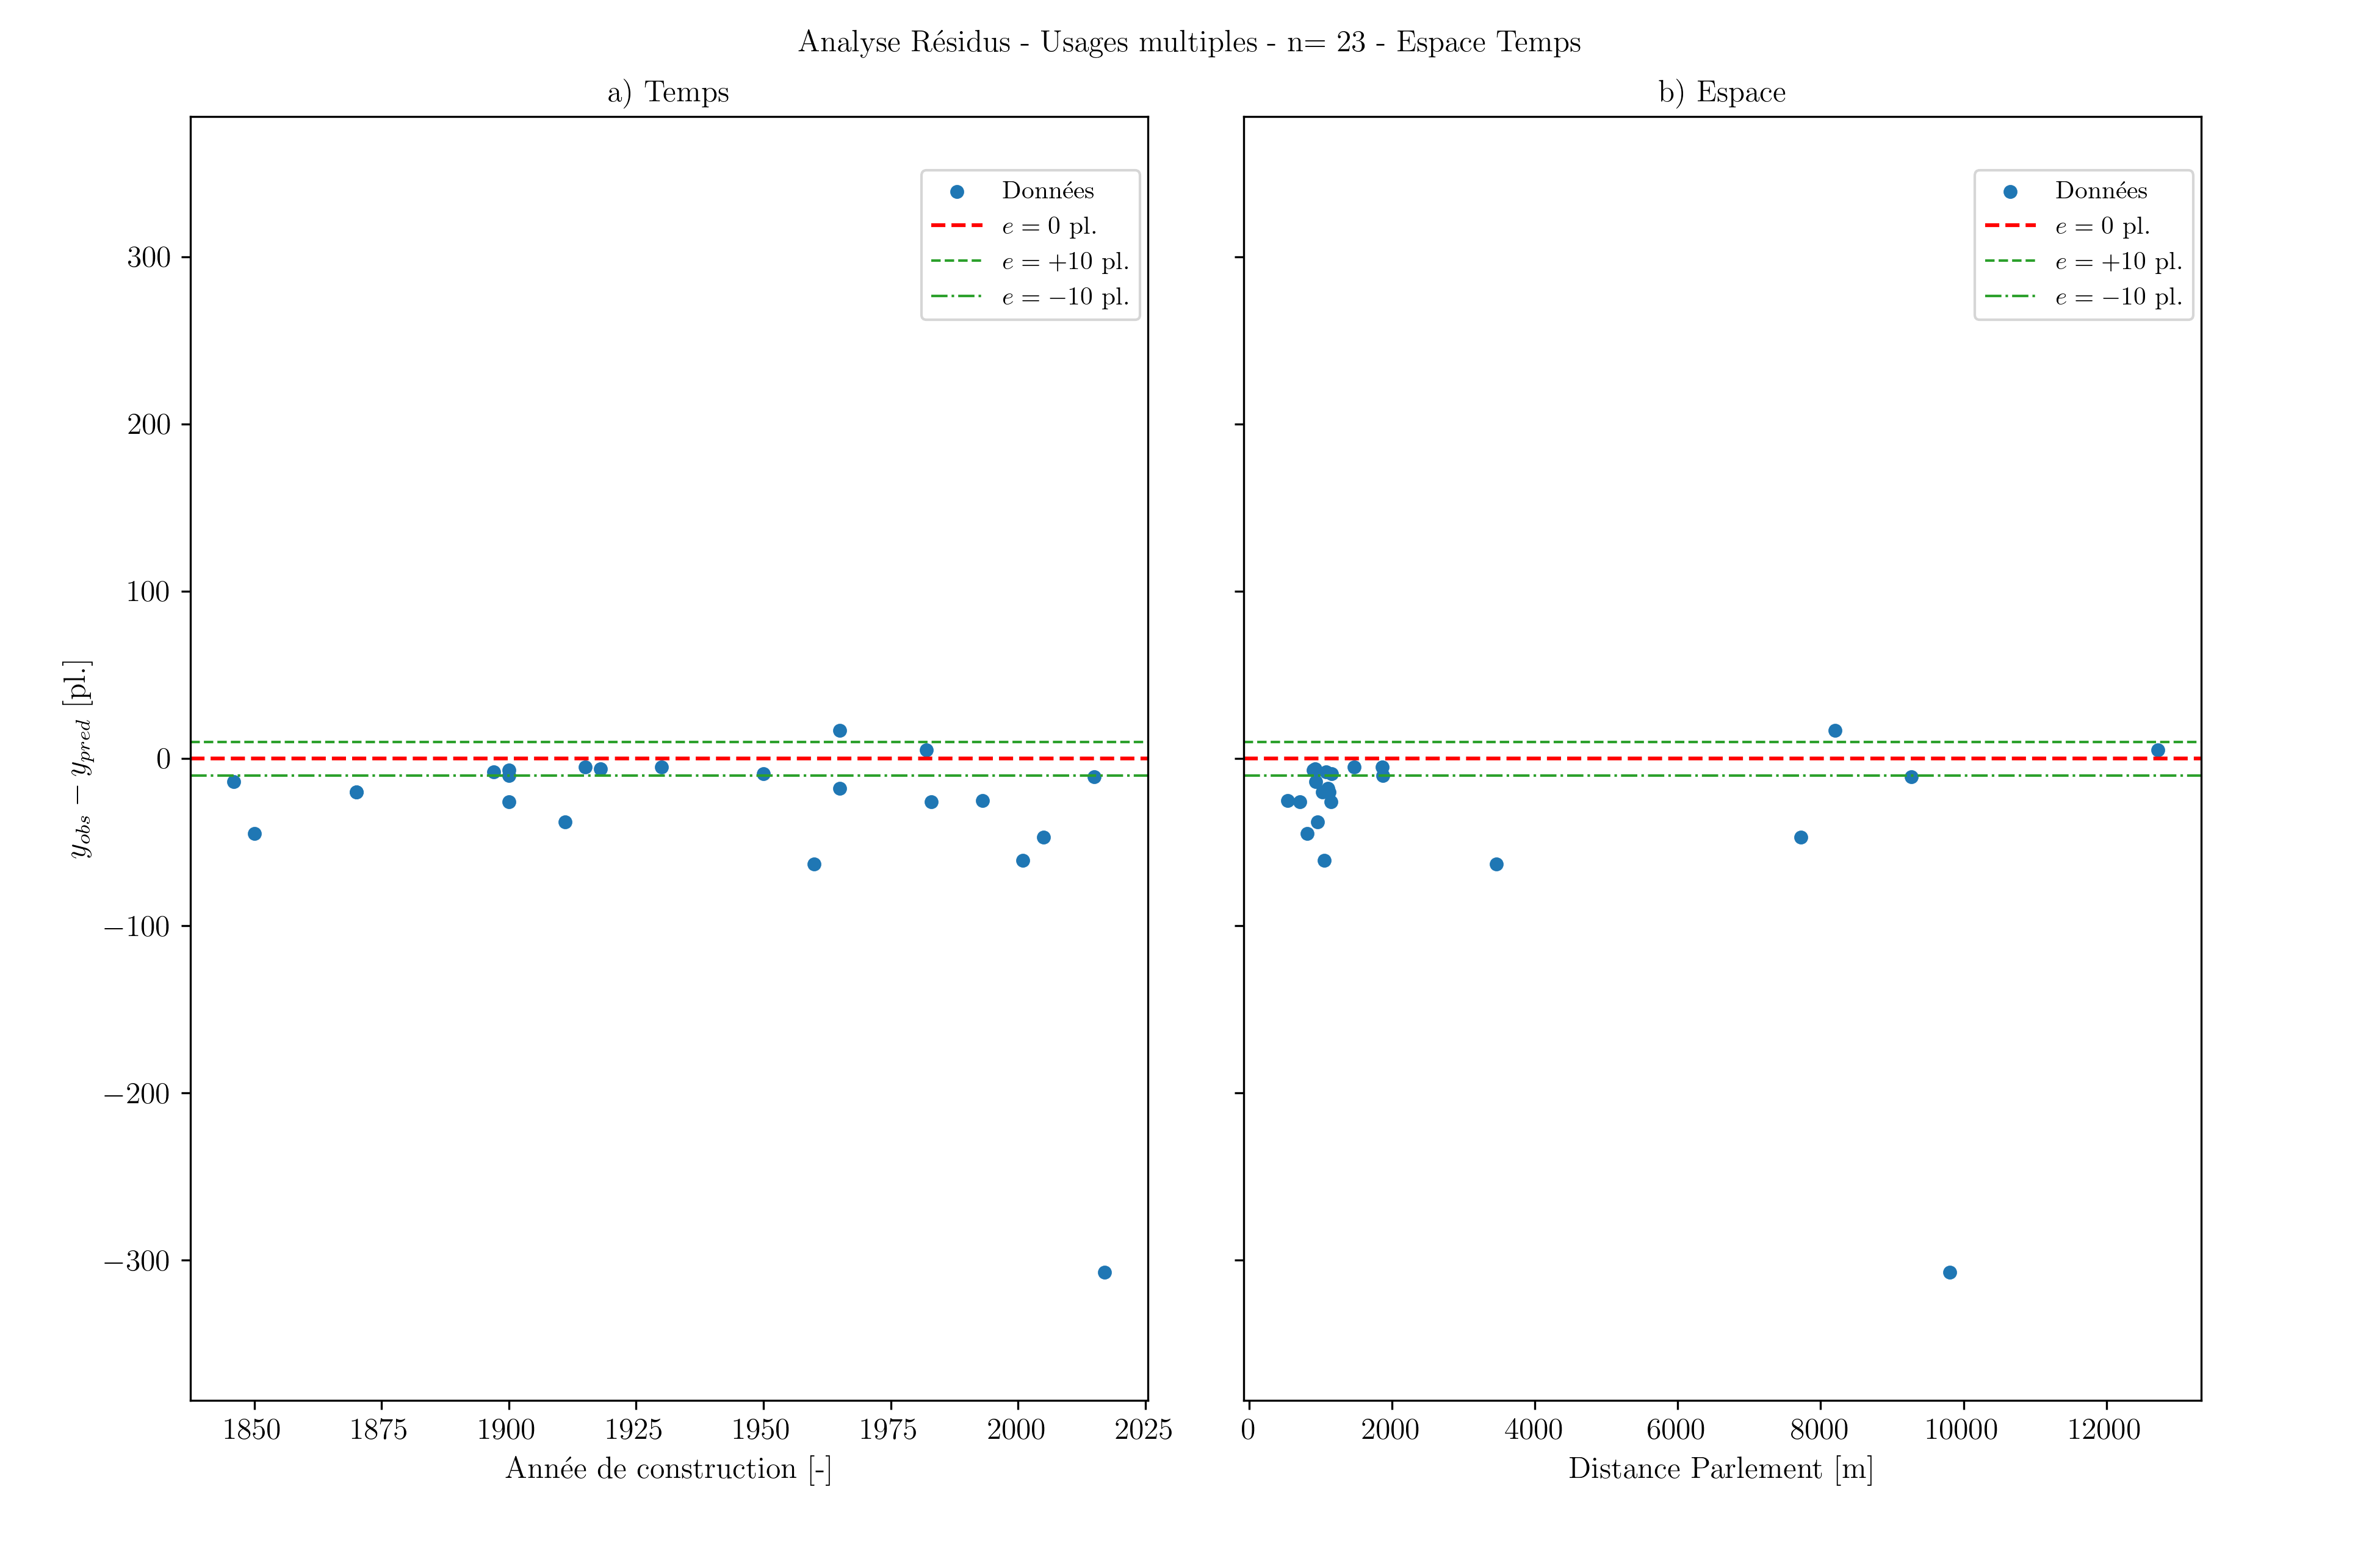
\includegraphics[width=1\linewidth]{images/ana_res_34_se_10_pe_20_b.png}
        \caption{Analyse des résidus en fonction de l'espace et de l'époque de construction pour les lots d'usage mixte}
        \label{fig:ana-res-esp-temps-mix}
    \end{figure}
    \begin{figure}[H]
        \centering
        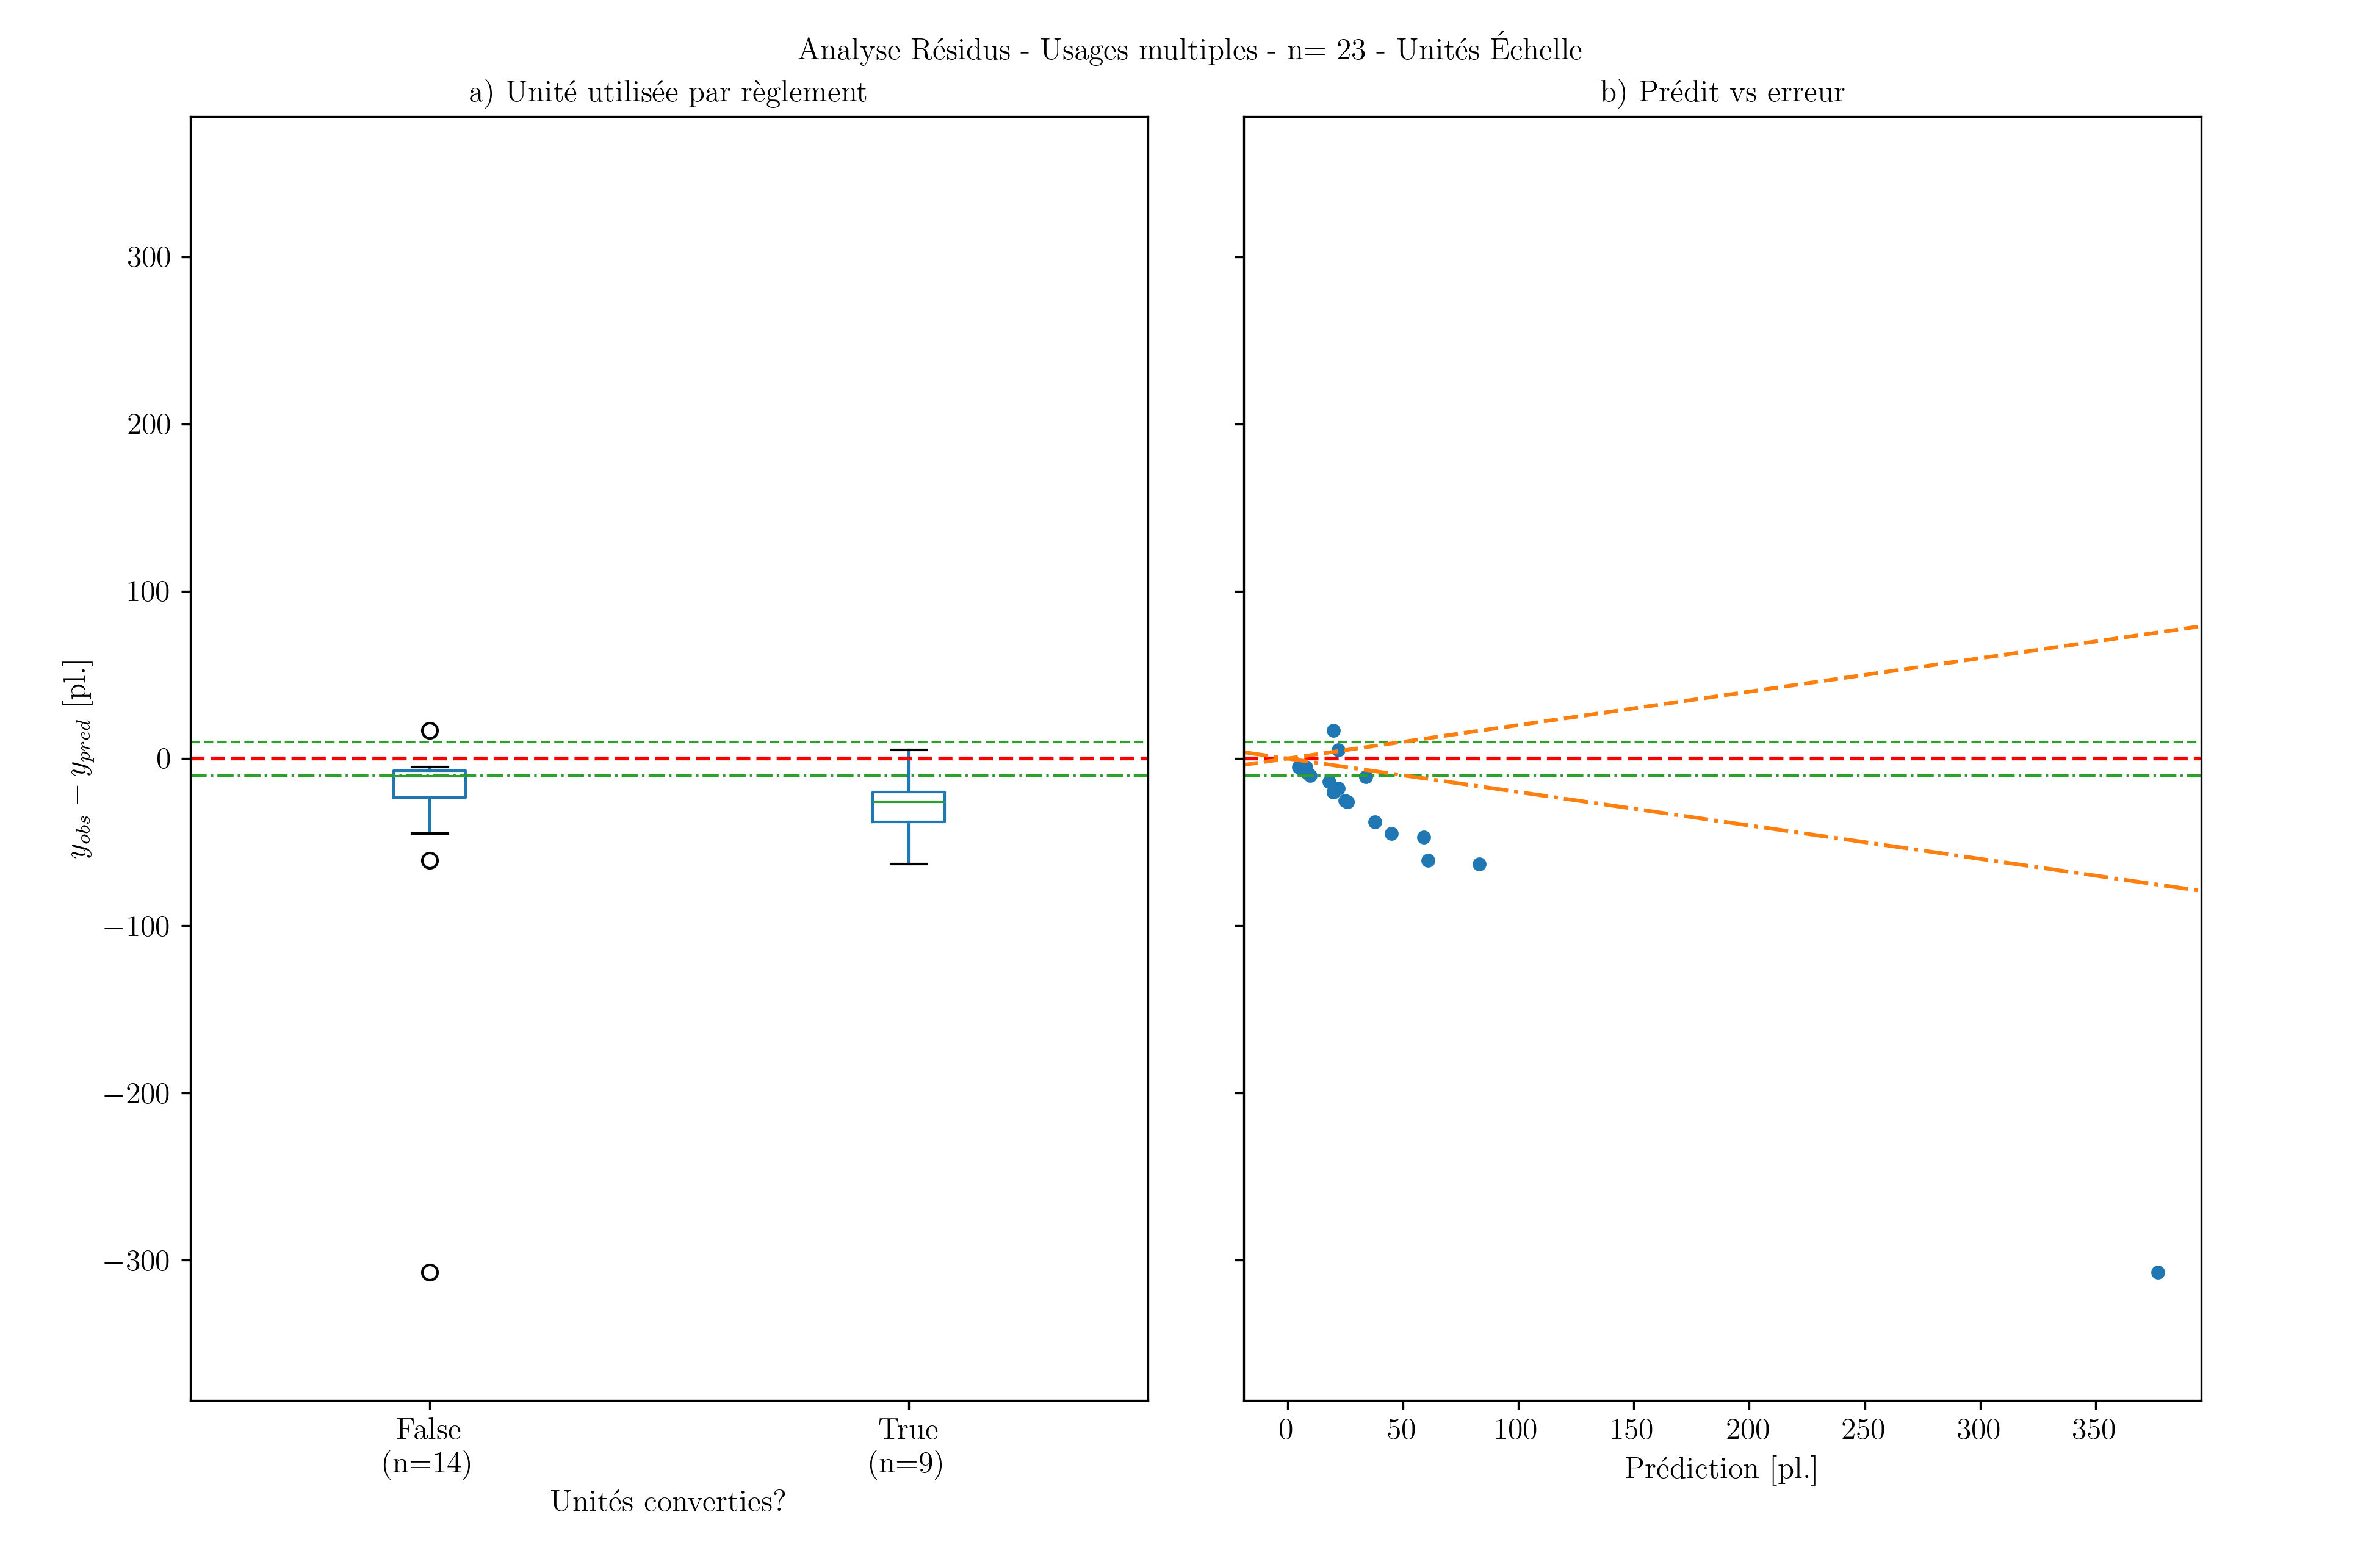
\includegraphics[width=1\linewidth]{images/ana_res_34_se_10_pe_20_c.png}
        \caption{Analyse des résidus en fonction de la prédiction et des unités de formulation pour les lots d'usage mixte}
        \label{fig:ana-res-unit-pred-mix}
    \end{figure}
    \begin{figure}[H]
        \centering
        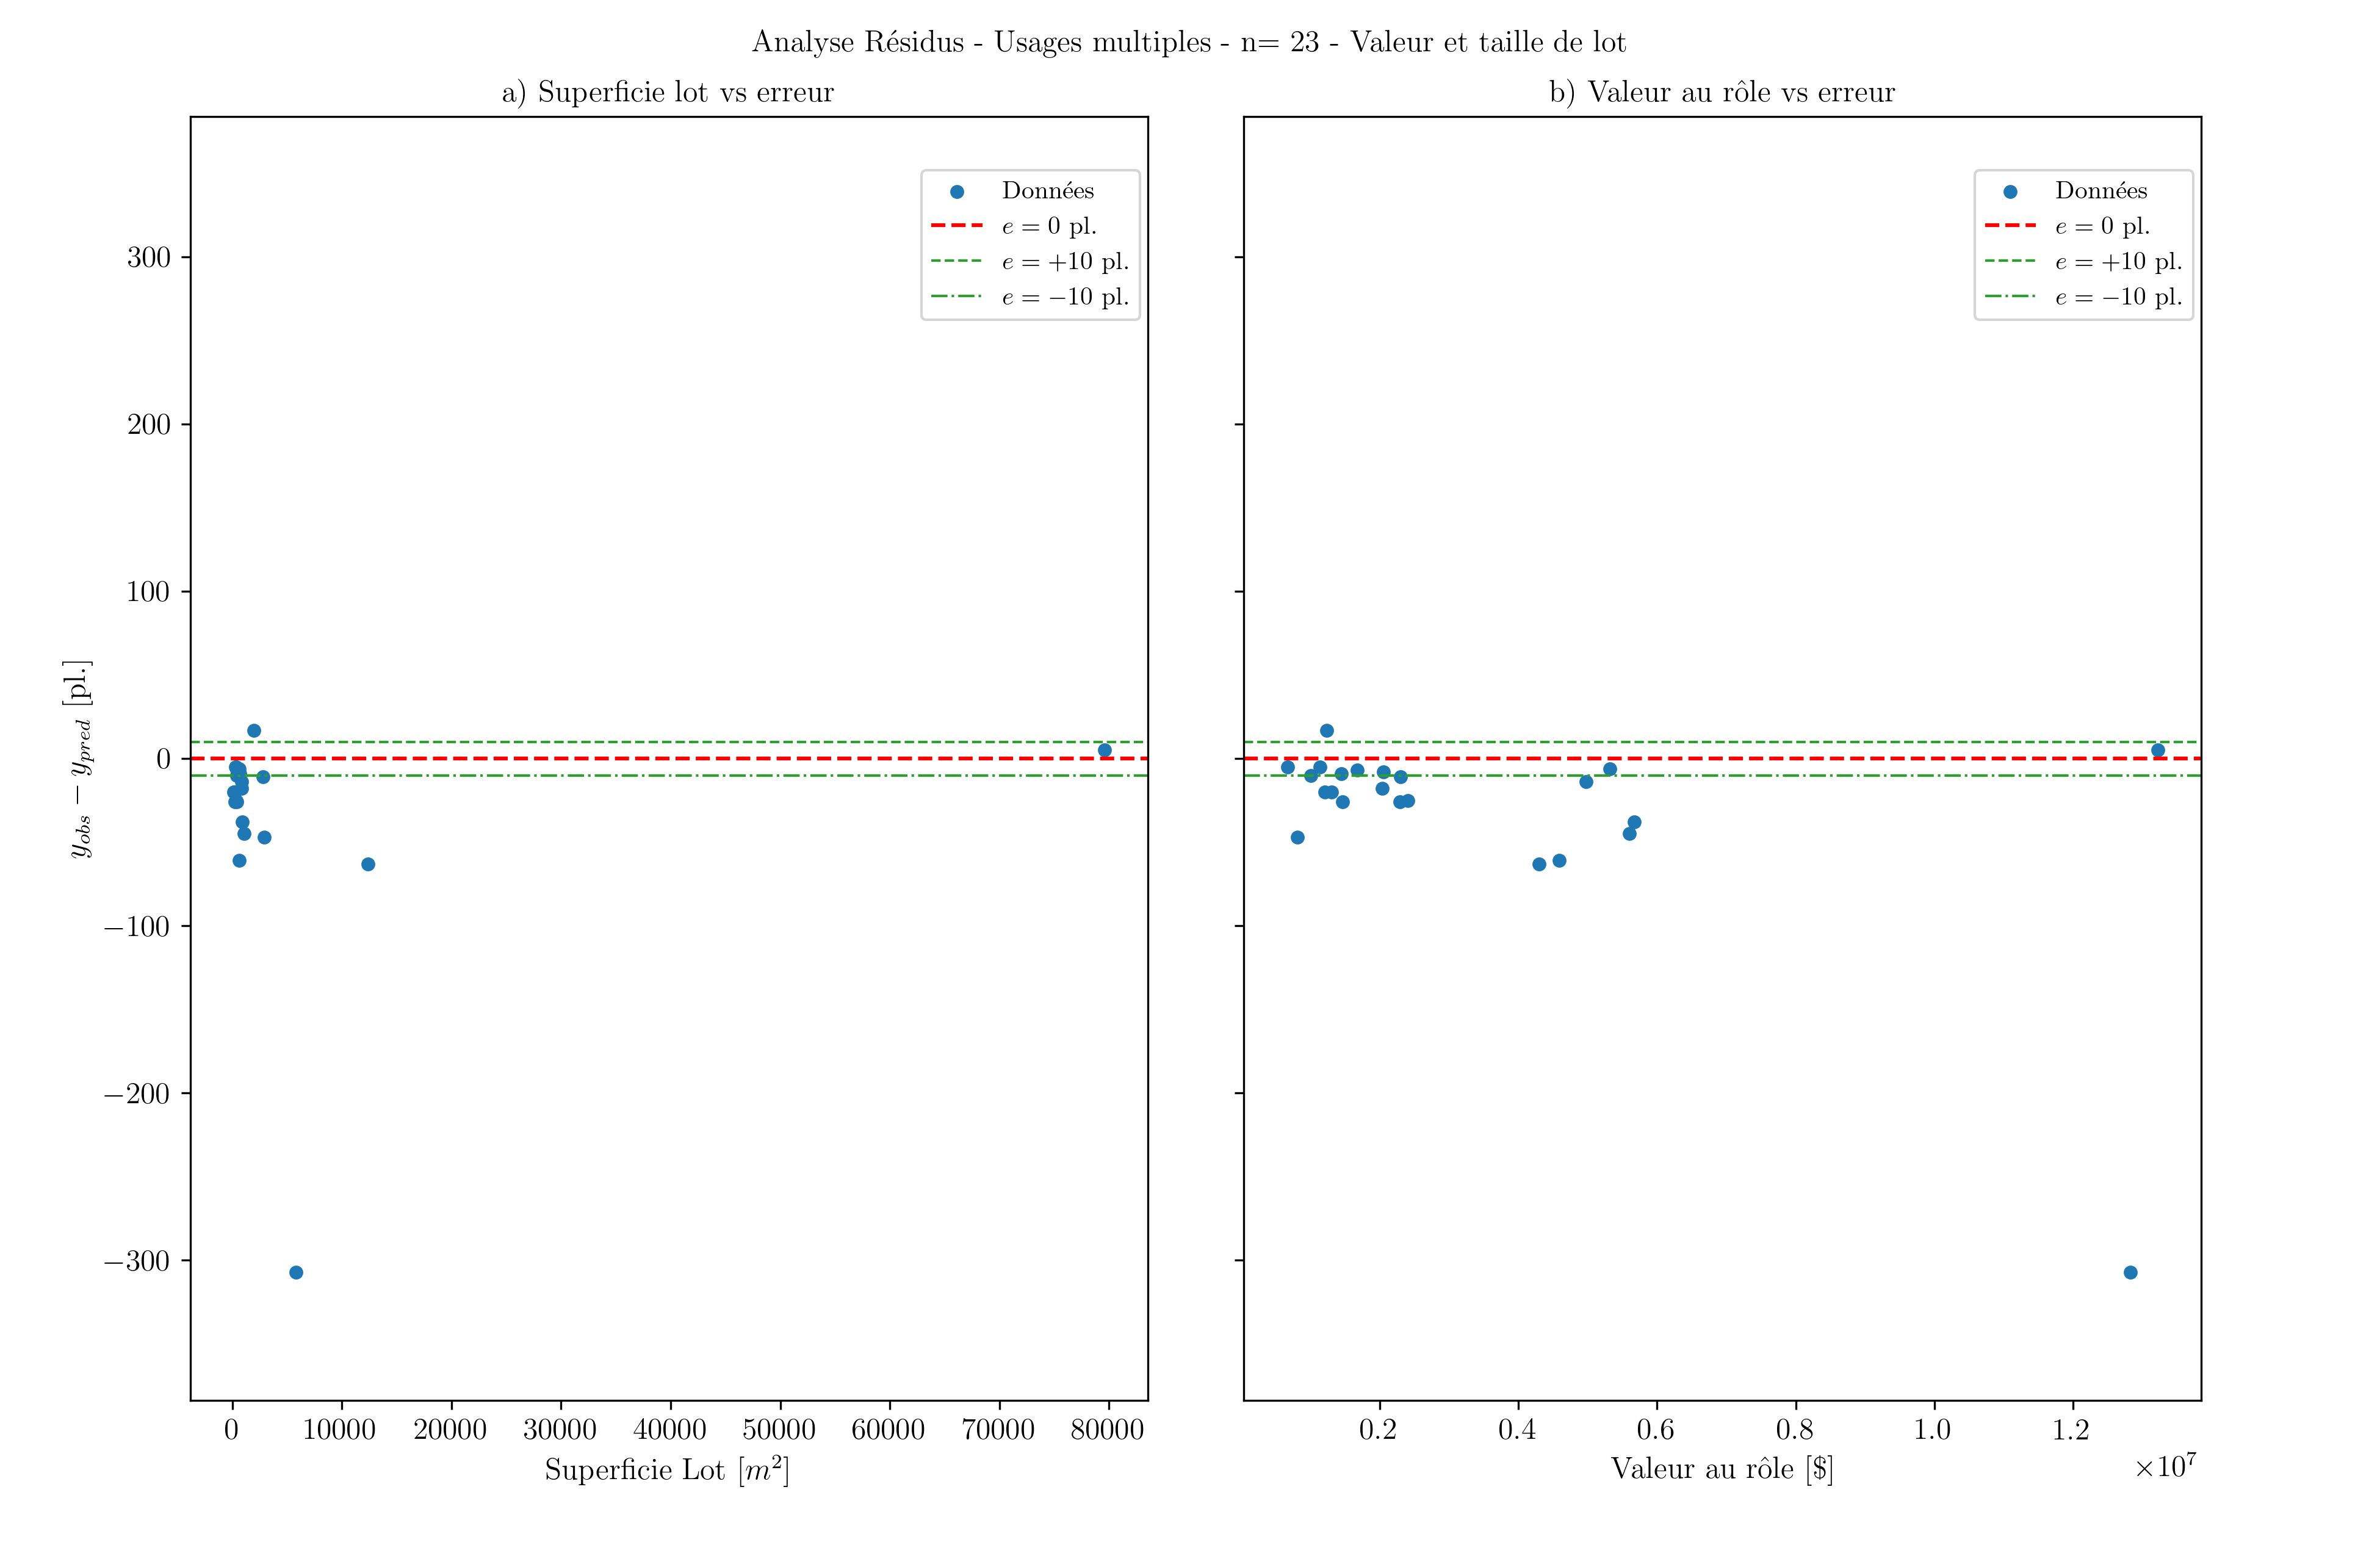
\includegraphics[width=1\linewidth]{images/ana_res_34_se_10_pe_20_d.png}
        \caption{Analyse des résidus en fonction de la superficie du lot et de la valeur pour les lots d'usage mixte}
        \label{fig:ana-res-sup-val-mix}
    \end{figure}
    \begin{figure}
        \centering
        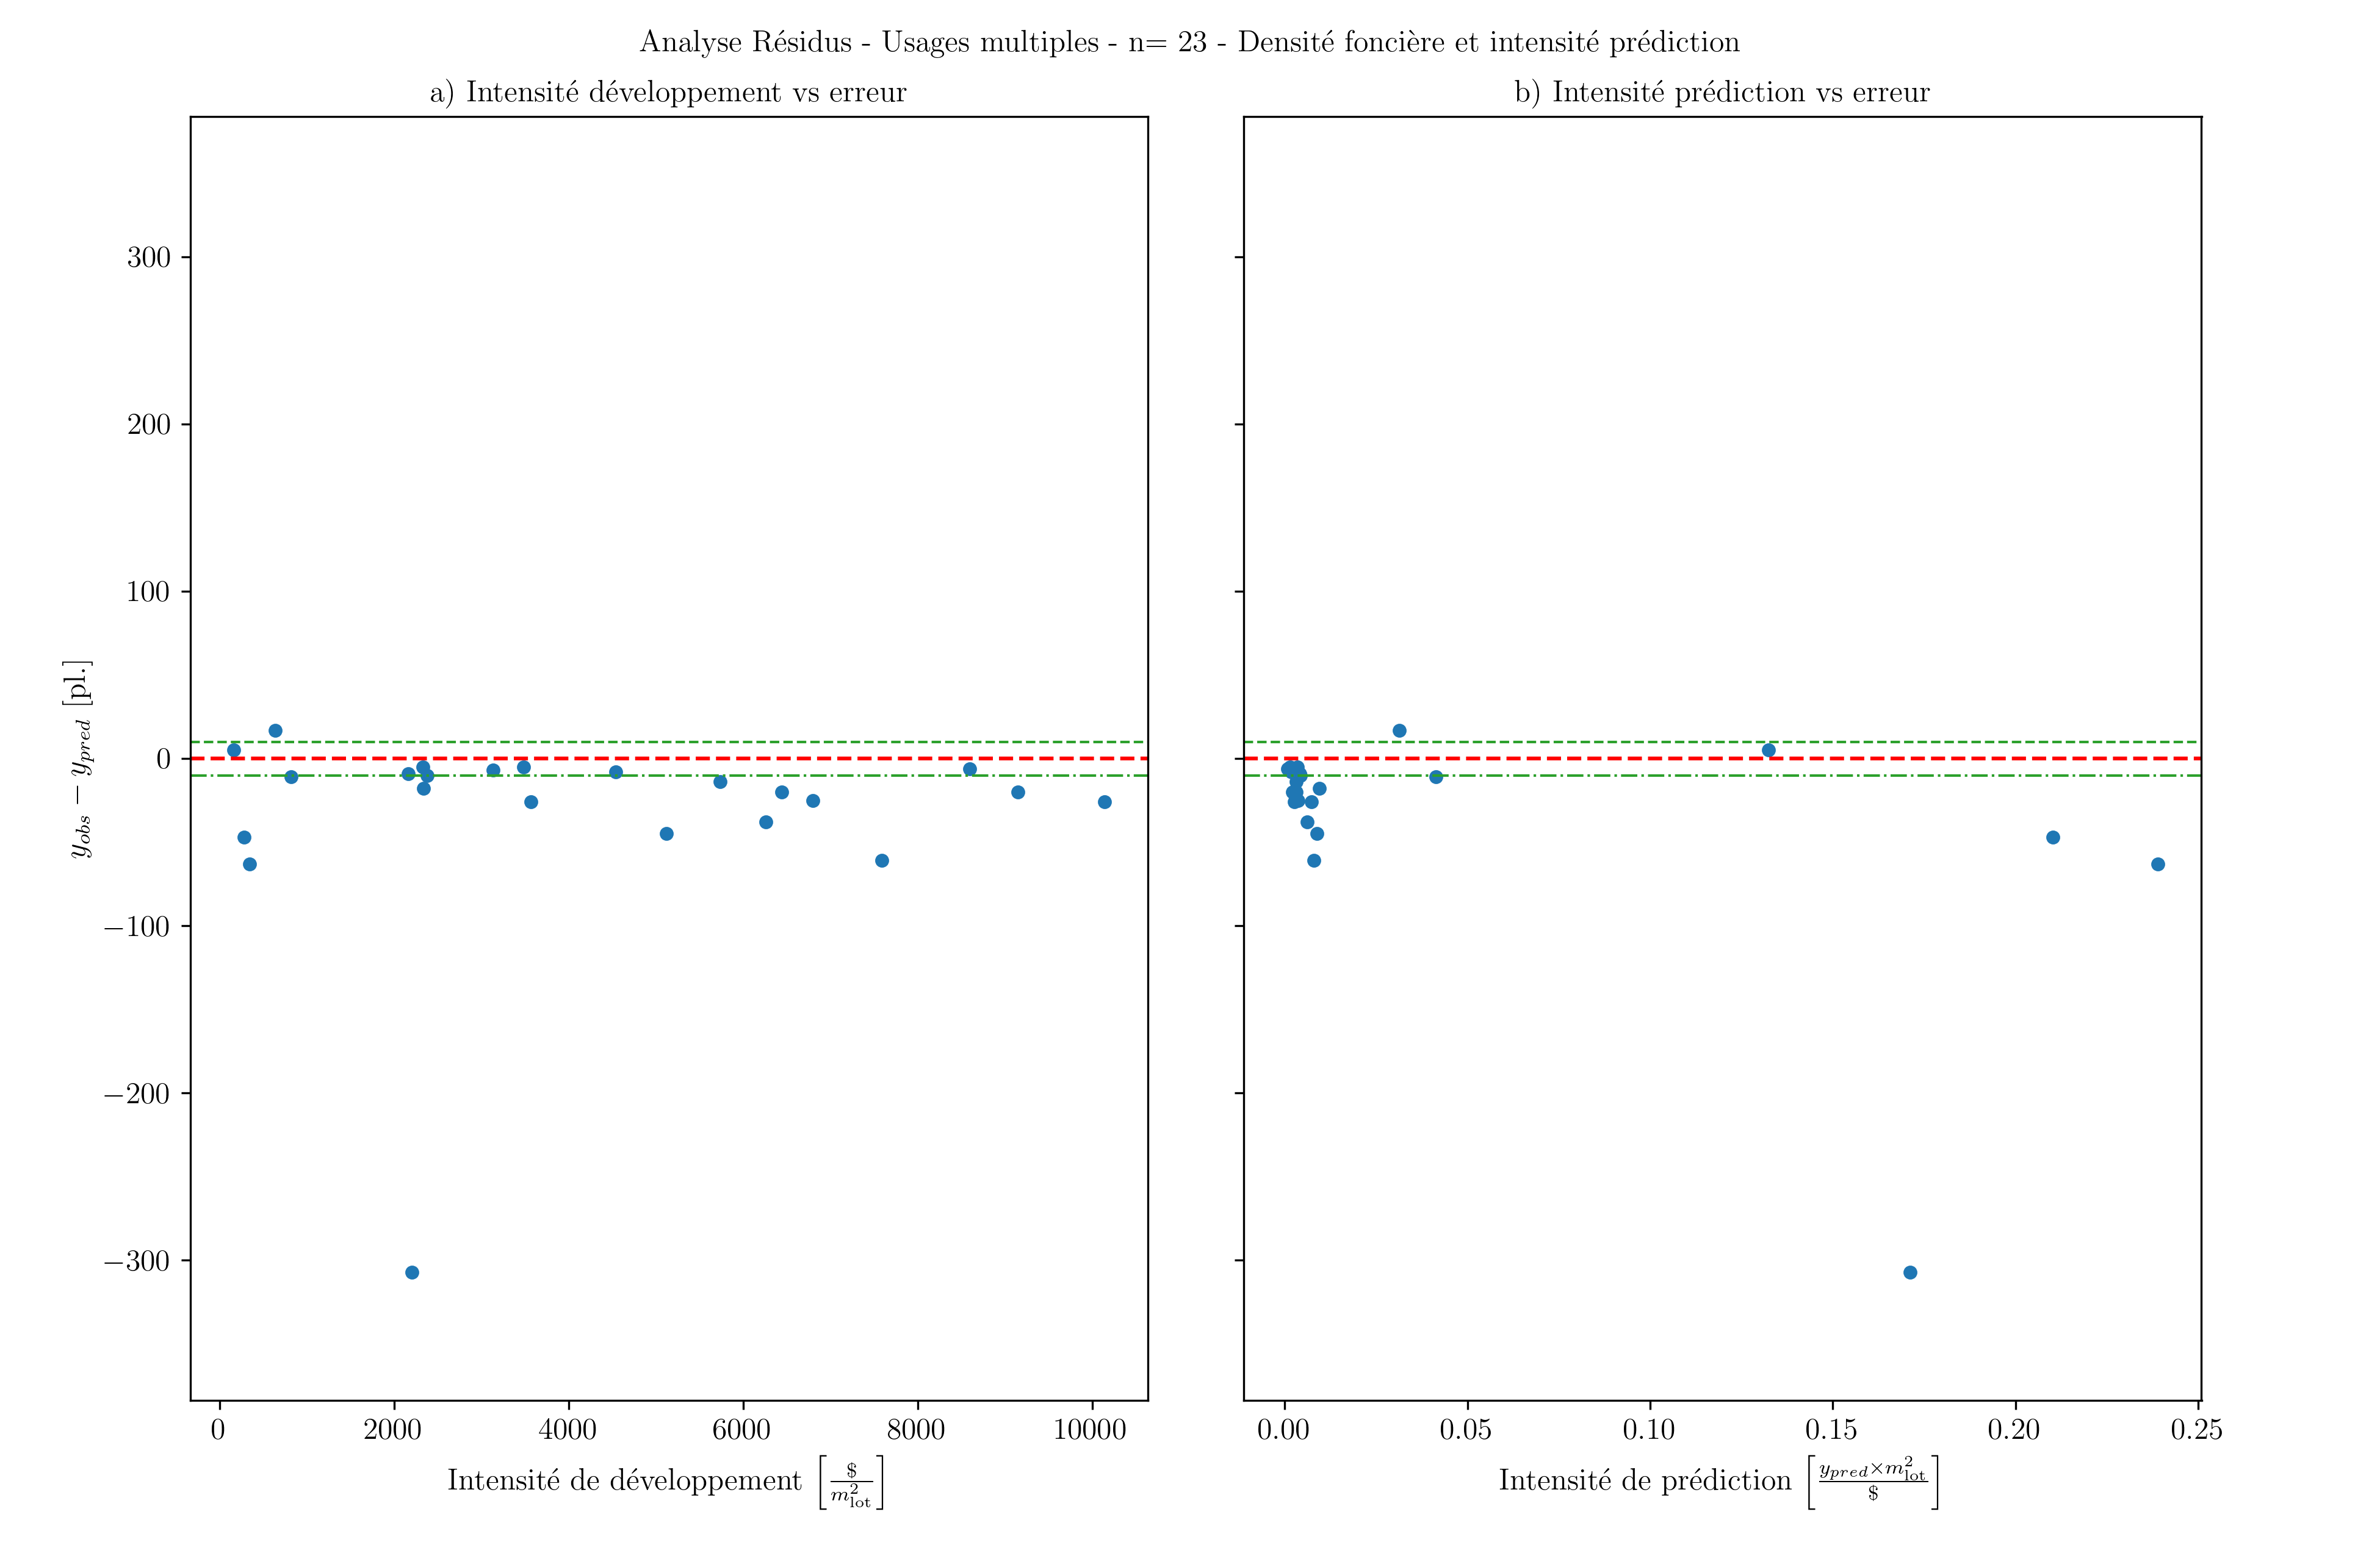
\includegraphics[width=0.95\linewidth]{images/ana_res_34_se_10_pe_20_e.png}
        \caption{Analyse des résidus en fonction de l'intensité de développement et l'intensité de prédiction pour les lots d'usage mixte}
        \label{fig:ana-res-intens-mix}
    \end{figure}
\end{landscape}
Ceci conclut la section sur la validation du modèle de prédiction. D'importants enjeux demeurent sur la précision des prédictions; les enjeux entourant les conversions d'unités sont principalement reliés à un modèle trop peu flexible pour accommoder la formulation des définitions, ainsi qu'une absence de processus de calibration formel. D'autres enjeux demeurent en dehors de la précision des hypothèses. Les données manquantes illustrées à la figure \ref{fig:role-missing-data} demeurent un frein majeur à l'émission de prédictions sur l'ensemble du territoire. La dernière section de ce chapitre discutera rapidement des relevés manuels et de prédictions semi-automatiques qui ont été complétées puis illustrera la manière dont les données pourraient être utilisées.